% Welcome to openmp.tex. This is the master LaTex file for the OpenMP specification.
%
% The files in this set include:
%
%    openmp.tex              - this file, the master file
%    Makefile                    - makes the document
%    openmp.sty                  - the main style file
%    openmp-index.ist            - the index style file
%    titlepage.tex               - the title page
%    ch*.tex                     - the main chapters
%    appendix*.tex               - the appendices
%    worksharing-schedule-loop.* - a flow chart diagram
%    openmplogo.png              - the logo
%
% When editing this file:
%
%    1. To change formatting, appearance, or style, please edit openmp.sty.
%
%    2. Custom commands and macros are defined in openmp.sty.
%
%    3. Be kind to other editors -- keep a consistent style by copying-and-pasting to
%       create new content.
%
%    4. We use semantic markup, e.g. (see openmp.sty for a full list):
%         \code{}     % for bold monospace keywords, code, operators, etc.
%         \plc{}      % for italic placeholder names, grammar, etc.
%
%    5. There are environments that provide special formatting, e.g. language bars.
%       Please use them whereever appropriate.  Examples are:
%
%         \begin{fortranspecific}
%         This is text that appears enclosed in blue language bars for Fortran.
%         \end{fortranspecific}
%
%         \begin{note}
%         This is a note.  The "Note -- " header appears automatically.
%         \end{note}
%
%    6. Other recommendations:
%         Use the convenience macros defined in openmp.sty for the minor headers
%         such as Comments, Syntax, etc.
%
%         To keep items together on the same page, prefer the use of
%         \begin{samepage}.... Avoid \parbox for text blocks as it interrupts line numbering.
%         When possible, avoid \filbreak, \pagebreak, \newpage, \clearpage unless that's
%         what you mean. Use \needspace{} cautiously for troublesome paragraphs.
%
%         Avoid absolute lengths and measures in this file; use relative units when possible.
%         Vertical space can be relative to \baselineskip or ex units. Horizontal space
%         can be relative to \linewidth or em units.
%
%         Prefer \emph{} to italicize terminology, e.g.:
%             This is a \emph{definition}, not a placeholder.
%             This is a \plc{var-name}.
%

% The following says letter size, but the style sheet may change the size
\documentclass[10pt,letterpaper,twoside,makeidx,hidelinks]{scrbook}

% Text to appear in the footer on even-numbered pages:
\newcommand{\footerText}{OpenMP API -- Version 5.0 rev 1, November 2016}

% Style sheet:
% This is openmp.sty, the preamble and style definitions for the OpenMP specification.
% This is an include file. Please see the master file for more information.
%
% When editing this file:
%
%    1. To change formatting, appearance, or style, please edit openmp.sty.
%
%    2. Custom commands and macros are defined in openmp.sty.
%
%    3. Be kind to other editors -- keep a consistent style by copying-and-pasting to
%       create new content.
%
%    4. We use semantic markup, e.g. (see openmp.sty for a full list):
%         \code{}     % for bold monospace keywords, code, operators, etc.
%         \plc{}      % for italic placeholder names, grammar, etc.
%
%    5. Other recommendations:
%         Use the convenience macros defined in openmp.sty for the minor headers
%         such as Comments, Syntax, etc.
%
%         To keep items together on the same page, prefer the use of 
%         \begin{samepage}.... Avoid \parbox for text blocks as it interrupts line numbering.
%         When possible, avoid \filbreak, \pagebreak, \newpage, \clearpage unless that's
%         what you mean. Use \needspace{} cautiously for troublesome paragraphs.
%
%         Avoid absolute lengths and measures in this file; use relative units when possible.
%         Vertical space can be relative to \baselineskip or ex units. Horizontal space
%         can be relative to \linewidth or em units.
%
%         Prefer \emph{} to italicize terminology, e.g.:
%             This is a \emph{definition}, not a placeholder.
%             This is a \plc{var-name}.
%
% Quick list of the environments, commands and macros supported. Search below for more details.
%
%    \binding                   % makes header of the same name
%    \comments
%    \constraints
%    \crossreferences
%    \descr
%    \effect
%    \format
%    \restrictions
%    \summary
%    \syntax
%    
%    \code{}                    % monospace, bold
%    \plc{}                     % for any kind of placeholder: italic
%    \begin{codepar}            % for blocks of verbatim code: monospace, bold
%    \begin{boxedcode}          % outlined verbatim code for syntax definitions, prototypes, etc.
%    \begin{indentedcodelist}   % used with,e.g., "where clause is one of the following:"
%
%    \specref{}                 % formats the cross-reference "Section X on page Y"
%    
%    \notestart                 % black horizontal rule for Notes
%    \noteend
%    
%    \cspecificstart            % blue horizontal rule for C-specific text
%    \cspecificend
%    
%    \cppspecificstart          % blue horizontal rule for C++ -specific text
%    \cppspecificend
%    
%    \ccppspecificstart         % blue horizontal rule for C / C++ -specific text
%    \ccppspecificend
%    
%    \fortranspecificstart      % blue horizontal rule for Fortran-specific text
%    \fortranspecificend
%    
%    \glossaryterm              % for use in formatting glossary entries
%    \glossarydefstart
%    \glossarydefend
%
%    \compactitem               % single-spaced itemized lists for the Examples doc
%    \cexample                  % C/C++ code example for the Examples doc
%    \fexample                  % Fortran code example for the Examples doc


\usepackage{comment}            % allow use of \begin{comment}
\usepackage{ifpdf,ifthen}       % allow conditional tests in LaTeX definitions
\usepackage{color,fancyvrb}  % for \VerbatimInput
\usepackage{xparse} %for argument passing to boxedcode


%%%%%%%%%%%%%%%%%%%%%%%%%%%%%%%%%%%%%%%%%%%%%%%%%%%%%%%%%%%%%%%%%%%%%%%%%%%%%%%%%%%%%%%%%%%%%%
% Document data
%
\author{}


%%%%%%%%%%%%%%%%%%%%%%%%%%%%%%%%%%%%%%%%%%%%%%%%%%%%%%%%%%%%%%%%%%%%%%%%%%%%%%%%%%%%%%%%%%%%%
% Fonts

\usepackage{amsmath}
\usepackage{amsfonts}
\usepackage{amssymb}
\usepackage{bm}
\usepackage{courier}
\usepackage{helvet}
\usepackage[utf8]{inputenc}

% Main body serif font:
\usepackage{tgtermes}
\usepackage[T1]{fontenc}


%%%%%%%%%%%%%%%%%%%%%%%%%%%%%%%%%%%%%%%%%%%%%%%%%%%%%%%%%%%%%%%%%%%%%%%%%%%%%%%%%%%%%%%%%%%%%
% Graphic elements

\usepackage{graphicx}
\usepackage{framed}    % for making boxes with \begin{framed}
\usepackage{tikz}      % for flow charts, diagrams, arrows
\usepackage{backnaur}  % for BNF grammar


%%%%%%%%%%%%%%%%%%%%%%%%%%%%%%%%%%%%%%%%%%%%%%%%%%%%%%%%%%%%%%%%%%%%%%%%%%%%%%%%%%%%%%%%%%%%%
% Page formatting

\usepackage[paperwidth=7.5in, paperheight=9in, 
            top=0.75in, bottom=1.0in, left=1.4in, right=0.6in]{geometry}

\usepackage{changepage}   % allows left/right-page margin readjustments

\setlength{\oddsidemargin}{0.45in}
\setlength{\evensidemargin}{0.185in}
\raggedbottom


%%%%%%%%%%%%%%%%%%%%%%%%%%%%%%%%%%%%%%%%%%%%%%%%%%%%%%%%%%%%%%%%%%%%%%%%%%%%%%%%%%%%%%%%%%%%%
% Paragraph formatting

\usepackage{setspace}     % allows use of \singlespacing, \onehalfspacing
\usepackage{needspace}    % allows use of \needspace to keep lines together
\usepackage{parskip}      % removes paragraph indenting

\raggedright
\usepackage[raggedrightboxes]{ragged2e}  % is this needed?

\lefthyphenmin=60         % only hyphenate if the left part is >= this many chars
\righthyphenmin=60        % only hyphenate if the right part is >= this many chars


%%%%%%%%%%%%%%%%%%%%%%%%%%%%%%%%%%%%%%%%%%%%%%%%%%%%%%%%%%%%%%%%%%%%%%%%%%%%%%%%%%%%%%%%%%%%%%
% Bulleted (itemized) lists
%    Align bullets with section header
%    Align text left
%    Small bullets
%    \compactitem for single-spaced lists (used in the Examples doc)

\usepackage{enumitem}     % for setting margins on lists
\setlist{leftmargin=*}    % don't indent bullet items
\renewcommand{\labelitemi}{{\normalsize$\bullet$}} % bullet size

% There is a \compactitem defined in package parlist (and perhaps others), however,
% we'll define our own version of compactitem in terms of package enumitem that
% we already use:
\newenvironment{compactitem}
{\begin{itemize}[itemsep=-1.2ex]}
{\end{itemize}}


%%%%%%%%%%%%%%%%%%%%%%%%%%%%%%%%%%%%%%%%%%%%%%%%%%%%%%%%%%%%%%%%%%%%%%%%%%%%%%%%%%%%%%%%%%%%%%
% Tables

% This allows tables to flow across page breaks, headers on each new page, etc.
\usepackage{supertabular}
\usepackage{caption}


%%%%%%%%%%%%%%%%%%%%%%%%%%%%%%%%%%%%%%%%%%%%%%%%%%%%%%%%%%%%%%%%%%%%%%%%%%%%%%%%%%%%%%%%%%%%%
% Line numbering

\usepackage[pagewise]{lineno}       % for line numbers on left side of the page
\pagewiselinenumbers
\setlength\linenumbersep{6em}
\renewcommand\linenumberfont{\normalfont\small\sffamily}
\nolinenumbers            % start with line numbers off


%%%%%%%%%%%%%%%%%%%%%%%%%%%%%%%%%%%%%%%%%%%%%%%%%%%%%%%%%%%%%%%%%%%%%%%%%%%%%%%%%%%%%%%%%%%%%
% Footers

\usepackage{fancyhdr}     % makes right/left footers
\pagestyle{fancy}
\fancyhead{} % clear all header fields
\cfoot{}
\renewcommand{\headrulewidth}{0pt}

% Left side on even pages:
% This requires that \footerText be defined in the master document:
\fancyfoot[LE]{\bfseries \thepage \mdseries \hspace{2em} \footerText}
\fancyhfoffset[E]{4em}

% Right side on odd pages:
\fancyfoot[RO]{\mdseries  \leftmark \hspace{2em} \bfseries \thepage}


%%%%%%%%%%%%%%%%%%%%%%%%%%%%%%%%%%%%%%%%%%%%%%%%%%%%%%%%%%%%%%%%%%%%%%%%%%%%%%%%%%%%%%%%%%%%%
% Section header format - we use four levels: \chapter \section \subsection \subsubsection.

\usepackage{titlesec}     % format headers with \titleformat{}

% Format and spacing for chapter, section, subsection, and subsubsection headers:

\setcounter{secnumdepth}{4}          % show numbers down to subsubsection level

\titleformat{\chapter}[display]%
{\normalfont\sffamily\upshape\Huge\bfseries\fontsize{20}{20}\selectfont}%
{\normalfont\sffamily\scshape\large\bfseries \hspace{-0.7in} \MakeUppercase%
    {\chaptertitlename} \thechapter}%
{0.8in}{}[\vspace{2ex}\hrule]
\titlespacing{\chapter}{0ex}{0em plus 1em minus 1em}{3em plus 1em minus 1em}[10em]

\titleformat{\section}[hang]{\huge\bfseries\sffamily\fontsize{16}{16}\selectfont}{\thesection}{1.0em}{}
\titlespacing{\section}{-5em}{5em plus 1em minus 1em}{1em plus 0.5em minus 0em}[10em]

\titleformat{\subsection}[hang]{\LARGE\bfseries\sffamily\fontsize{14}{14}\selectfont}{\thesubsection}{1.0em}{}
\titlespacing{\subsection}{-5em}{4em plus 1em minus 2.0em}{0.75em plus 0.5em minus 0em}[10em]

\titleformat{\subsubsection}[hang]{\needspace{1\baselineskip}%
\Large\bfseries\sffamily\fontsize{12}{12}\selectfont}{\thesubsubsection}{1.0em}{}
\titlespacing{\subsubsection}{-5em}{3em plus 1em minus 1em}{0.5em plus 0.5em minus 0em}[10em]


%%%%%%%%%%%%%%%%%%%%%%%%%%%%%%%%%%%%%%%%%%%%%%%%%%%%%%%%%%%%%%%%%%%%%%%%%%%%%%%%%%%%%%%%%%%%%%
% Macros for minor headers: Summary, Syntax, Description, etc.
% These headers are defined in terms of \paragraph

\titleformat{\paragraph}[block]{\large\bfseries\sffamily\fontsize{11}{11}\selectfont}{}{}{}
\titlespacing{\paragraph}{0em}{1.5em plus 0.55em minus 0.5em}{0.0em plus 0.55em minus 0.0em}

% Use one of the convenience macros below, or \littleheader{} for an arbitrary header
\newcommand{\littleheader}[1] {\paragraph*{#1}}

\newcommand{\binding} {\littleheader{Binding}}
\newcommand{\comments} {\littleheader{Comments}}
\newcommand{\constraints} {\littleheader{Constraints on Arguments}}
\newcommand{\crossreferences} {\littleheader{Cross References}}
\newcommand{\descr} {\littleheader{Description}}
\newcommand{\effect} {\littleheader{Effect}}
\newcommand{\format} {\littleheader{Format}}
\newcommand{\restrictions} {\littleheader{Restrictions}}
\newcommand{\summary} {\littleheader{Summary}}
\newcommand{\syntax} {\littleheader{Syntax}}
\newcommand{\tools} {\littleheader{Tools Interface}}


%%%%%%%%%%%%%%%%%%%%%%%%%%%%%%%%%%%%%%%%%%%%%%%%%%%%%%%%%%%%%%%%%%%%%%%%%%%%%%%%%%%%%%%%%%%%%%
% Code and placeholder semantic tagging.
%
% When possible, prefer semantic tags instead of typographic tags. The
% following semantics tags are defined here:
%
%     \code{}     % for bold monospace keywords, code, operators, etc.
%     \plc{}      % for italic placeholder names, grammar, etc.
%
% For function prototypes or other code snippets, you can use \code{} as
% the outer wrapper, and use \plc{{} inside. Example:
%
%     \code{\#pragma omp directive ( \plc{some-placeholder-identifier} :}
%
% To format text in italics for emphasis (rather than text as a placeholder),
% use the generic \emph{} command. Example:
%
%     This sentence \emph{emphasizes some non-placeholder words}.
% Enable \alltt{} for formatting blocks of code:
\usepackage{alltt}
\usepackage{listings}

% This sets the default \code{} font to tt (monospace) and bold:
\RecustomVerbatimCommand{\verb}{Verb}{fontseries=b, commandchars=\\\{\}}
\newcommand{\code}[1]{{\texttt{\textbf{#1}}}}
\newcommand{\nspace}[1]{{\textrm{\textmd{ }}}}

% This defines the \plc{} placeholder font to be tt normal slanted:
\newcommand{\plc}[1] {{\textrm{\textmd{\itshape{#1}}}}}

% Environment for a paragraph of literal code, single-spaced, no outline, no indenting:
\newenvironment{codepar}[1]
{\begin{alltt}\bfseries #1}
{\end{alltt}}

% For blocks of code inside a box frame:
\DefineVerbatimEnvironment{OMPVerbatim}{Verbatim}{fontseries=b, commandchars=\\\{\}}
\newenvironment{boxedcode}
{ \VerbatimEnvironment
  \vspace{0.25em plus 5em minus 0.25em}
  \begin{framed}
  \begin{minipage}[t]{\textwidth}
  \begin{OMPVerbatim}
  }
  {
  \end{OMPVerbatim}
\end{minipage}\end{framed}\vspace{0.25em plus 5em minus 0.25em}}

% This sets the margins in the framed box:
\setlength{\FrameSep}{0.6em}

% For indented lists of verbatim code at a relaxed line spacing,
% e.g., for use after "where clause is one of the following:"
\usepackage{setspace}
\newenvironment{indentedcodelist}{%
    \begin{adjustwidth}{0.25in}{}\begin{spacing}{1.5}\begin{alltt}\bfseries}
    {\end{alltt}\end{spacing}\vspace{-0.25\baselineskip}\end{adjustwidth}}


%%%%%%%%%%%%%%%%%%%%%%%%%%%%%%%%%%%%%%%%%%%%%%%%%%%%%%%%%%%%%%%%%%%%%%%%%%%%%%%%%%%%%%%%%%%%%%
% Macros for the black and blue lines and arrows delineating language-specific
% and notes sections. Example:
%
%   \fortranspecificstart
%   This is text that applies to Fortran.
%   \fortranspecificend

% local parameters for use \linewitharrows and \notelinewitharrows:
\newlength{\sbsz}\setlength{\sbsz}{0.05in}  % size of arrows
\newlength{\sblw}\setlength{\sblw}{1.35pt}  % line width (thickness)
\newlength{\sbtw}                           % text width
\newlength{\sblen}                          % total width of horizontal rule
\newlength{\sbht}                           % height of arrows
\newlength{\sbhadj}                         % vertical adjustment for aligning arrows with the line
\newlength{\sbns}\setlength{\sbns}{7\baselineskip}       % arg for \needspace for downward arrows

% \notelinewitharrows is a helper command that makes a black Note marker:
%     arg 1 = 1 or -1 for up or down arrows
%     arg 2 = solid or dashed or loosely dashed, etc.
\newcommand{\notelinewitharrows}[2]{%
    \needspace{0.1\baselineskip}%
    \vbox{\begin{tikzpicture}%
        \setlength{\sblen}{\linewidth}%
        \setlength{\sbht}{#1\sbsz}\setlength{\sbht}{1.4\sbht}%
        \setlength{\sbhadj}{#1\sblw}\setlength{\sbhadj}{0.25\sbhadj}%
        \filldraw (\sblen, 0) -- (\sblen - \sbsz, \sbht) -- (\sblen - 2\sbsz, 0) -- (\sblen, 0);
        \draw[line width=\sblw, #2] (2\sbsz - \sblw, \sbhadj) -- (\sblen - 2\sbsz + \sblw, \sbhadj);
        \filldraw (0, 0) -- (\sbsz, \sbht) -- (0 + 2\sbsz, 0) -- (0, 0);
    \end{tikzpicture}}}

% \linewitharrows is a helper command that makes a blue horizontal line, up or down arrows, and some text:
% arg 1 = 1 or -1 for up or down arrows
% arg 2 = solid or dashed or loosely dashed, etc.
% arg 3 = text
% arg 4 = text width
\newcommand{\linewitharrows}[4]{%
    \needspace{0.1\baselineskip}%
    \vbox to 1\baselineskip {\begin{tikzpicture}%
        \setlength{\sbtw}{#4}%
        \setlength{\sblen}{\linewidth}%
        \setlength{\sbht}{#1\sbsz}\setlength{\sbht}{1.4\sbht}%
        \setlength{\sbhadj}{#1\sblw}\setlength{\sbhadj}{0.25\sbhadj}%
        \filldraw[color=blue!40] (\sblen, 0) -- (\sblen - \sbsz, \sbht) -- (\sblen - 2\sbsz, 0) -- (\sblen, 0);
        \draw[line width=\sblw, color=blue!40, #2] (2\sbsz - \sblw, \sbhadj) -- (0.5\sblen - 0.5\sbtw, \sbhadj);
        \draw[line width=\sblw, color=blue!40, #2] (0.5\sblen + 0.5\sbtw, \sbhadj) -- (\sblen - 2\sbsz + \sblw, \sbhadj);
        \filldraw[color=blue!40] (0, 0) -- (\sbsz, \sbht) -- (0 + 2\sbsz, 0) -- (0, 0);
        \node[color=blue!90] at (0.5\sblen, 0) {\large  \textsf{\textup{#3}}};
    \end{tikzpicture}}}

\newcommand{\VSPb}{\vspace{0.5ex plus 5ex minus 0.25ex}}
\newcommand{\VSPa}{\vspace{0.25ex plus 5ex minus 0.25ex}}

% C
\newcommand{\cspecificstart}{\needspace{\sbns}\linewitharrows{-1}{solid}{C}{3em}}
\newcommand{\cspecificend}{\linewitharrows{1}{solid}{C}{3em}\bigskip}

% C/C++
\newcommand{\ccppspecificstart}{\VSPb\linewitharrows{-1}{solid}{C / C++}{6em}\VSPa}
\newcommand{\ccppspecificend}{\VSPb\linewitharrows{1}{solid}{C / C++}{6em}\VSPa}

% C++
\newcommand{\cppspecificstart}{\needspace{\sbns}\linewitharrows{-1}{solid}{C++}{6em}}
\newcommand{\cppspecificend}{\linewitharrows{1}{solid}{C++}{6em}\bigskip}

% C90
\newcommand{\cNinetyspecificstart}{\needspace{\sbns}\linewitharrows{-1}{solid}{C90}{4em}}
\newcommand{\cNinetyspecificend}{\linewitharrows{1}{solid}{C90}{4em}\bigskip}

% C99
\newcommand{\cNinetyNinespecificstart}{\needspace{\sbns}\linewitharrows{-1}{solid}{C99}{4em}}
\newcommand{\cNinetyNinespecificend}{\linewitharrows{1}{solid}{C99}{4em}\bigskip}

% Fortran
\newcommand{\fortranspecificstart}{\VSPb\linewitharrows{-1}{solid}{Fortran}{6em}\VSPa}
\newcommand{\fortranspecificend}{\VSPb\linewitharrows{1}{solid}{Fortran}{6em}\VSPa}

% Note
\newcommand{\notestart}{\VSPb\notelinewitharrows{-1}{solid}\VSPa}
\newcommand{\noteend}{\VSPb\notelinewitharrows{1}{solid}\VSPa}

% convenience macro for formatting the word "Note:" at the beginning of note blocks:
\newcommand{\noteheader}{{\textrm{\textsf{\textbf\textup\normalsize{{{{Note }}}}}}}}


%%%%%%%%%%%%%%%%%%%%%%%%%%%%%%%%%%%%%%%%%%%%%%%%%%%%%%%%%%%%%%%%%%%%%%%%%%%%%%%%%%%%%%%%%%%%%%
% Glossary formatting

\newcommand{\glossaryterm}[1]{\needspace{1ex}
\begin{adjustwidth}{-0.75in}{0.0in}
\nolinenumbers\parbox[b][-0.95\baselineskip][t]{1.4in}{\flushright \textbf{#1}}
\end{adjustwidth}\linenumbers}

\newcommand{\glossarydefstart}{
\begin{adjustwidth}{0.79in}{0.0in}}

\newcommand{\glossarydefend}{
\end{adjustwidth}\vspace{-1.5\baselineskip}}


%%%%%%%%%%%%%%%%%%%%%%%%%%%%%%%%%%%%%%%%%%%%%%%%%%%%%%%%%%%%%%%%%%%%%%%%%%%%%%%%%%%%%%%%%%%%%
% Indexing and Table of Contents

\usepackage{makeidx}
\usepackage[nodotinlabels]{titletoc}   % required for its [nodotinlabels] option

% Clickable links in TOC and index:
\usepackage[hyperindex=true,linktocpage=true]{hyperref}
\hypersetup{
  colorlinks  = true, % Colors links instead of red boxes
  urlcolor    = blue, % Color for external links
  linkcolor   = blue  % Color for internal links
}


%%%%%%%%%%%%%%%%%%%%%%%%%%%%%%%%%%%%%%%%%%%%%%%%%%%%%%%%%%%%%%%%%%%%%%%%%%%%%%%%%%%%%%%%%%%%%
% Formats a cross reference label as "Section X on page Y".

\newcommand{\specref}[1]{Section~\ref{#1} on page~\pageref{#1}}

% Formats a cross reference label as "Chapter X on page Y".

\newcommand{\specchapterref}[1]{Chapter~\ref{#1} on page~\pageref{#1}}

% For caption for supertabular and figure, by yanyh15
\captionsetup[table]{labelfont={sf,sc,bf},textfont=normalfont,singlelinecheck=off,labelformat=simple,labelsep=colon,aboveskip=00pt,belowskip=10pt}
% \renewcommand{\thetable}{\thechapter-\arabic{table}}
%
\captionsetup[figure]{labelfont={sf,sc,bf},textfont=normalfont,singlelinecheck=off,labelformat=simple,labelsep=colon}
% \renewcommand{\thefigure}{\thechapter-\arabic{figure}}
%
%%%%%%%%%%%%%%%%%%%%%%%%%%%%%%%%%%%%%%%%%%%%%%%%%%%%%%%%%%%%%%%%%%%%%%%%%%%%%%%%%%%%%%%%%%%%%
% Code example formatting for the Examples document
% This defines:
%     /cexample       formats blue markers, caption, and code for C/C++ examples
%     /fexample       formats blue markers, caption, and code for Fortran examples
% Thanks to Jin, Haoqiang H. for the original definitions of the following:

\usepackage{toolbox}         % for \toolboxMakeSplit

\newcommand{\myreplace}[3]{\bgroup\toolboxMakeSplit*{#1}{DoSplit}%
   \long\def\DoReplace##1{\DoSplit{##1}\lefttext\righttext
   \lefttext
   \toolboxIfElse{\ifx\righttext\undefined}{}%
      {#2\expandafter\DoReplace\expandafter{\righttext}}}%
   \DoReplace{#3}\egroup}

\newcommand{\escstr}[1]{\myreplace{_}{\_}{#1}}

\def\exampleheader#1#2{%
   \ifthenelse{ \equal{#1}{} }{
      \def\cname{#2}
      \def\ename\cname
   }{
      \def\cname{#1.#2}
% Use following line for old numbering
%      \def\ename{\thesection.#2}
% Use following for mneumonics
      \def\ename{\escstr{#1}.#2}
   }
   \noindent
   \textit{Example \ename}
   %\vspace*{-3mm}
}

\def\cnexample#1#2{%
   \exampleheader{#1}{#2}
   %\code{\VerbatimInput[numbers=left,numbersep=14ex,firstnumber=\thelinenumber,firstline=8,fontsize=\small]%
   %\code{\VerbatimInput[numbers=left,firstnumber=1,firstline=8,fontsize=\small]%
   \code{\VerbatimInput[firstline=8,fontsize=\small]%
      {sources/Example_\cname.c}} 
}

\def\fnexample#1#2{%
   \exampleheader{#1}{#2}
   %\code{\VerbatimInput[numbers=left,numbersep=14ex,firstnumber=\thelinenumber,firstline=6,fontsize=\small]%
   %\code{\VerbatimInput[numbers=left,firstnumber=1,firstline=8,fontsize=\small]%
   \code{\VerbatimInput[firstline=8,fontsize=\small]%
      {sources/Example_\cname.f}}
}

\newcommand\cexample[2]{%
\needspace{5\baselineskip}\ccppspecificstart
\cnexample{#1}{#2}
\ccppspecificend
}

\newcommand\fexample[2]{%
\needspace{5\baselineskip}\fortranspecificstart
\fnexample{#1}{#2}
\fortranspecificend
}

% Commands for "bold" ceiling and floor symbols

\newcommand\blfloor{\bm{\lfloor\mkern-10mu\lfloor}}
\newcommand\brfloor{\bm{\rfloor\mkern-10mu\rfloor}}
\newcommand\blceil{\bm{\lceil\mkern-10mu\lceil}}
\newcommand\brceil{\bm{\rceil\mkern-10mu\rceil}}

% Set default fonts:
\rmfamily\mdseries\upshape\normalsize


% This is the end of openmp.sty of the OpenMP specification.


% Enable the next line to display labels and cross-references for debugging:
%\usepackage{showkeys}

\makeindex

\begin{document}
    \pagenumbering{roman}
    %%%%%%%%%%%%%%%%%%%%%%%%%%%%%%%%%%%%%%%%%%%%%%%%%%%%%%%%%%%%%%%%%%%%%%%%%%%%%%%%%%%%%%%%%%%%%%
% Title page

  \begin{titlepage}
    \begin{flushleft}
     \hspace{-6em} 
\includegraphics[width=0.4\textwidth]{openmp-logo.png}
    \end{flushleft}

    \begin{adjustwidth}{-0.75in}{0in}
    \begin{center}
      \Huge
      \textsf{OpenMP\\Application Programming\\Interface}

      % An optional subtitle can go here:
      \vspace{0.5in}\textsf{    }\vspace{-0.7in}
      \normalsize

      \vspace{1.0in}

      \textbf{Version 5.0 Public Comment Draft, July 2018}
    \end{center}
    \end{adjustwidth}

    \vspace{3.0in}

\begin{adjustwidth}{0pt}{1em}\setlength{\parskip}{0.25\baselineskip}%
Copyright \copyright 1997-2018 OpenMP Architecture Review Board.\\
Permission to copy without fee all or part of this material is granted,
provided the OpenMP Architecture Review Board copyright notice and
the title of this document appear. Notice is given that copying is by
permission of OpenMP Architecture Review Board.\end{adjustwidth}

  \end{titlepage}

% Blank page

\clearpage
\thispagestyle{empty}
\phantom{a}
This page intentionally left blank in published version.

%% Commented out for official release.
This is Revision 3-TR7 (Third Official Draft) (12 July 2018) and
includes the following internal tickets applied to the 4.5 LaTeX sources:
50, 134, 354, 389, 399, 408, 425, 426, 430, 445, 452, 458, 459, 461-463, 
465-467, 484, 486, 489-504, 508, 510, 511, 514, 518, 520, 521, 523, 
524, 530-533, 536, 539, 542, 545, 546, 548, 551, 555-562, 564, 568-578, 
581-586, 589-592, 594, 597, 598, 601, 603, 604, 606, 608-618, 620-646, 
648-651, 654-656, 659, 661-666, 668-673, 675-677, 679-681, 684-686, 
691-696, 699-712, 715, 717-723, 725-736, 738, 740, 745, 748-778, 780-790, 
794, 796, 797, 799-803, 821, 822, 828, 829, 831, 832

%% DO NOT DISTRIBUTE
This is a draft; contents will change in official release.
%% This is an internal draft; contents will change in official release

\vfill



    \setcounter{page}{0}

% Four levels in Toc  e.g.  2.14.3.2  (rchrd)
%    \setcounter{tocdepth}{3}

    \begin{spacing}{1.3}
        \tableofcontents
    \end{spacing}
    \cleardoublepage

    \linenumbers\pagewiselinenumbers
    \newpage\pagenumbering{arabic}

    % This is introduction.tex (Chapter 1 )of the OpenMP specification
% This is an included file. See the master file for more information.
%
% When editing this file:
%
%    1. To change formatting, appearance, or style, please edit openmp.sty.
%
%    2. Custom commands and macros are defined in openmp.sty.
%
%    3. Be kind to other editors -- keep a consistent style by copying-and-pasting to
%       create new content.
%
%    4. We use semantic markup, e.g. (see openmp.sty for a full list):
%         \code{}     % for bold monospace keywords, code, operators, etc.
%         \plc{}      % for italic placeholder names, grammar, etc.
%
%    5. There are environments that provide special formatting, e.g. language bars.
%       Please use them whereever appropriate.  Examples are:
%
%         \begin{fortranspecific}
%         This is text that appears enclosed in blue language bars for Fortran.
%         \end{fortranspecific}
%
%         \begin{note}
%         This is a note.  The "Note -- " header appears automatically.
%         \end{note}
%
%    6. Other recommendations:
%         Use the convenience macros defined in openmp.sty for the minor headers
%         such as Comments, Syntax, etc.
%
%         To keep items together on the same page, prefer the use of 
%         \begin{samepage}.... Avoid \parbox for text blocks as it interrupts line numbering.
%         When possible, avoid \filbreak, \pagebreak, \newpage, \clearpage unless that's
%         what you mean. Use \needspace{} cautiously for troublesome paragraphs.
%
%         Avoid absolute lengths and measures in this file; use relative units when possible.
%         Vertical space can be relative to \baselineskip or ex units. Horizontal space
%         can be relative to \linewidth or em units.
%
%         Prefer \emph{} to italicize terminology, e.g.:
%             This is a \emph{definition}, not a placeholder.
%             This is a \plc{var-name}.
%

\chapter{Introduction}
\index{introduction}
\label{chap:introduction}
The collection of compiler directives, library routines, and environment
variables described in this document collectively define the specification of
the OpenMP Application Program Interface (OpenMP API) for parallelism in C, C++
and Fortran programs.

This specification provides a model for parallel programming that is portable
across architectures from different vendors. Compilers from numerous vendors
support the OpenMP API. More information about the OpenMP API can be found at
the following web site

\code{http://www.openmp.org}

The directives, library routines, and environment variables defined in this document 
allow users to create and to manage parallel programs while permitting portability. The 
directives extend the C, C++ and Fortran base languages with single program multiple 
data (SPMD) constructs, tasking constructs, device constructs, worksharing constructs, 
and synchronization constructs, and they provide support for sharing, mapping and privatizing 
data. The functionality to control the runtime environment is provided by library 
routines and environment variables. Compilers that support the OpenMP API often 
include a command line option to the compiler that activates and allows interpretation of 
all OpenMP directives.







\section{Scope}
\label{sec:Scope}
The OpenMP API covers only user-directed parallelization, wherein the programmer 
explicitly specifies the actions to be taken by the compiler and runtime system in order 
to execute the program in parallel. OpenMP-compliant implementations are not required 
to check for data dependencies, data conflicts, race conditions, or deadlocks, any of 
which may occur in conforming programs. In addition, compliant implementations are 
not required to check for code sequences that cause a program to be classified as 
non-conforming. Application developers are responsible for correctly using the OpenMP API 
to produce a conforming program. The OpenMP API does not cover compiler-generated 
automatic parallelization and directives to the compiler to assist such parallelization.







\section{Glossary}
\label{sec:Glossary}
\index{glossary}
\subsection{Threading Concepts}
\label{subsec:Threading Concepts}
\glossaryterm{thread}
\glossarydefstart
An execution entity with a stack and associated static memory, called 
\emph{threadprivate memory}.
\glossarydefend

\glossaryterm{OpenMP thread}
\glossarydefstart
A \emph{thread} that is managed by the OpenMP runtime system.
\glossarydefend

\glossaryterm{idle thread}
\glossarydefstart
An \emph{OpenMP thread} that is not currently part of any \code{parallel} region. 
\glossarydefend

\glossaryterm{thread-safe routine}
\glossarydefstart
A routine that performs the intended function even when executed concurrently 
(by more than one \emph{thread}).
\glossarydefend

\glossaryterm{processor}
\glossarydefstart
Implementation defined hardware unit on which one or more \emph{OpenMP threads} can 
execute.
\glossarydefend

\glossaryterm{device}
\glossarydefstart
An implementation defined logical execution engine.

\begin{quote}
COMMENT: A \emph{device} could have one or more \emph{processors}.
\end{quote}
\glossarydefend

\glossaryterm{host device}
\glossarydefstart
The \emph{device} on which the \emph{OpenMP program} begins execution.
\glossarydefend

\glossaryterm{target device}
\glossarydefstart
A device onto which code and data may be offloaded from the \emph{host device}.
\glossarydefend





\subsection{OpenMP Language Terminology}
\label{subsec:OpenMP Language Terminology}
\glossaryterm{base language}
\glossarydefstart
A programming language that serves as the foundation of the OpenMP 
specification.

\begin{quote}
COMMENT: See \specref{sec:normative references}
for a listing of current \emph{base languages} for the OpenMP API.
\end{quote}
\glossarydefend

\glossaryterm{base program}
\glossarydefstart
A program written in a \emph{base language}.
\glossarydefend

\glossaryterm{program order}
\glossarydefstart
An ordering of operations performed by the same thread as determined by the
execution sequence of operations specified by the \emph{base language}.

\begin{quote}
COMMENT: For C11 and C++11, \emph{program order} corresponds to the sequenced
before relation between operations performed by the same thread.
\end{quote}
\glossarydefend

\glossaryterm{structured block}
\glossarydefstart
For C/C++, an executable statement, possibly compound, with a single entry at the 
top and a single exit at the bottom, or an OpenMP \emph{construct}.

For Fortran, a block of executable statements with a single entry at the top and a 
single exit at the bottom, or an OpenMP \emph{construct}.

\begin{quote}
COMMENTS:

For all \emph{base languages}:

\begin{itemize}
\item Access to the \emph{structured block} must not be the result of a branch; and

\item The point of exit cannot be a branch out of the \emph{structured block}.
\end{itemize}

For C/C++:

\begin{itemize}
\item The point of entry must not be a call to \code{setjmp()};

\item \code{longjmp()} and \code{throw()} must not violate the entry/exit criteria;

\item Calls to \code{exit()} are allowed in a \emph{structured block}; and

\item An expression statement, iteration statement, selection statement, 
or try block is considered to be a \emph{structured block} if the 
corresponding compound statement obtained by enclosing it in \code{\{} 
and \code{\}} would be a \emph{structured block}.
\end{itemize}

For Fortran:

\begin{itemize}
\item \code{STOP} statements are allowed in a \emph{structured block}.
\end{itemize}
\end{quote}
\glossarydefend


\glossaryterm{enclosing context}
\glossarydefstart
In C/C++, the innermost scope enclosing an OpenMP \emph{directive}.

In Fortran, the innermost scoping unit enclosing an OpenMP \emph{directive}.
\glossarydefend

\glossaryterm{directive}
\glossarydefstart
In C/C++, a \code{\#pragma}, and in Fortran, a comment, that specifies \emph{OpenMP
program} behavior.

\begin{quote}
COMMENT: See \specref{sec:Directive Format} for a description of OpenMP \emph{directive} syntax.
\end{quote}
\glossarydefend


\glossaryterm{white space}
\glossarydefstart
A non-empty sequence of space and/or horizontal tab characters.
\glossarydefend

\glossaryterm{OpenMP program}
\glossarydefstart
A program that consists of a \emph{base program}, annotated with OpenMP \emph{directives} and 
runtime library routines.
\glossarydefend

\glossaryterm{conforming program}
\glossarydefstart
An \emph{OpenMP program} that follows all rules and restrictions of the OpenMP 
specification.
\glossarydefend

\glossaryterm{declarative directive}
\glossarydefstart
An OpenMP \emph{directive} that may only be placed in a declarative context. A 
\emph{declarative directive} results in one or more declarations only; it is not associated 
with the immediate execution of any user code.
\glossarydefend

\glossaryterm{executable directive}
\glossarydefstart
An OpenMP \emph{directive} that is not declarative. That is, it may be placed in an 
executable context.
\glossarydefend

\glossaryterm{stand-alone directive}
\glossarydefstart
An OpenMP \emph{executable directive} that has no associated executable user code.
\glossarydefend


\glossaryterm{construct}
\glossarydefstart
An OpenMP \emph{executable directive} (and for Fortran, the paired \code{end} \emph{directive}, if 
any) and the associated statement, loop or \emph{structured block}, if any, not including 
the code in any called routines. That is, the lexical extent of an \emph{executable 
directive}.
\glossarydefend

\glossaryterm{combined construct}
\glossarydefstart
A construct that is a shortcut for specifying one construct immediately nested inside another construct. A combined construct is semantically identical to that of explicitly specifying the first construct containing one instance of the second construct and no other statements.
\glossarydefend

\glossaryterm{composite construct} 
\glossarydefstart 
A construct that is composed of two constructs but does not have identical semantics to specifying one of the constructs immediately nested inside the other. A composite construct either adds semantics not included in the constructs from which it is composed or the nesting of the one construct inside the other is not conforming.
\glossarydefend


\glossaryterm{region}
\glossarydefstart
All code encountered during a specific instance of the execution of a given 
\emph{construct} or of an OpenMP library routine. A \emph{region} includes any code in called 
routines as well as any implicit code introduced by the OpenMP implementation. 
The generation of a \emph{task} at the point where a \emph{task generating construct} is encountered is a 
part of the \emph{region} of the \emph{encountering thread}, but an \emph{explicit task region}
associated with a \emph{task generating construct} is not unless it is an
\emph{included task region}. The point where a \code{target} or \code{teams}
directive is encountered is a part of the \emph{region} of the \emph{encountering thread}, but the 
\emph{region} associated with the \code{target} or \code{teams} directive is not.

\begin{quote}
COMMENTS:

A \emph{region} may also be thought of as the dynamic or runtime extent of a 
\emph{construct} or of an OpenMP library routine.

During the execution of an \emph{OpenMP program}, a \emph{construct} may give 
rise to many \emph{regions}.
\end{quote}
\glossarydefend

\glossaryterm{active parallel region}
\glossarydefstart
A \code{parallel} \emph{region} that is executed by a \emph{team} consisting of more than one 
\emph{thread}.
\glossarydefend

\smallskip
\glossaryterm{inactive parallel region}
\glossarydefstart
A \code{parallel} \emph{region} that is executed by a \emph{team} of only one \emph{thread}.
\glossarydefend

\glossaryterm{sequential part}
\glossarydefstart
All code encountered during the execution of an \emph{initial task region} that is not part 
of a \code{parallel} \emph{region} corresponding to a \code{parallel} \emph{construct} or a \code{task}
\emph{region} corresponding to a \code{task} \emph{construct}.

\begin{quote}
COMMENTS: 

A \emph{sequential part} is enclosed by an \emph{implicit parallel region}.

Executable statements in called routines may be in both a \emph{sequential 
part} and any number of explicit \code{parallel} \emph{regions} at different points 
in the program execution.
\end{quote}
\glossarydefend

\glossaryterm{master thread}
\glossarydefstart
An \emph{OpenMP thread} that has  \emph{thread} number 0. A \emph{master
thread} may be an \emph{initial thread} or the \emph{thread} that encounters a
\code{parallel} \emph{construct}, creates a \emph{team}, generates a set of
\emph{implicit tasks}, and then executes one of those \emph{tasks} as
\emph{thread} number 0.
\glossarydefend

\glossaryterm{parent thread}
\glossarydefstart
The \emph{thread} that encountered the \code{parallel} \emph{construct} and generated a 
\code{parallel} \emph{region} is the \emph{parent thread} of each of the 
\emph{threads} in the \emph{team} of that 
\code{parallel} \emph{region}. The \emph{master thread} 
of a \code{parallel} \emph{region} is the same \emph{thread} 
as its \emph{parent thread} with respect to any resources associated with an \emph{OpenMP thread}.
\glossarydefend

\glossaryterm{child thread}
\glossarydefstart
When a thread encounters a \code{parallel} construct, each of the threads in the 
generated \code{parallel} region's team are \emph{child threads} of the encountering \emph{thread}. 
The \code{target} or \code{teams} region's \emph{initial thread} is not a \emph{child thread} of the thread 
that encountered the \code{target} or \code{teams} construct. 
\glossarydefend

\glossaryterm{ancestor thread}
\glossarydefstart
For a given \emph{thread}, its \emph{parent thread} or one of its \emph{parent thread’s ancestor threads}.
\glossarydefend

\glossaryterm{descendent thread}
\glossarydefstart
For a given \emph{thread}, one of its \emph{child threads} or one of 
its \emph{child threads’ descendent threads}.
\glossarydefend

\glossaryterm{team}
\glossarydefstart
A set of one or more \emph{threads} participating in the execution of a \code{parallel}
\emph{region}.

\begin{quote}
COMMENTS:

For an \emph{active parallel region}, the team comprises the \emph{master thread} 
and at least one additional \emph{thread}.

For an \emph{inactive parallel region}, the \emph{team} comprises only the \emph{master thread}.
\end{quote}
\glossarydefend

\glossaryterm{league}
\glossarydefstart
The set of \emph{thread teams} created by a \code{teams} construct.
\glossarydefend

\glossaryterm{contention group}
\glossarydefstart
An initial \emph{thread} and its \emph{descendent threads}.
\glossarydefend

\glossaryterm{implicit parallel region}
\glossarydefstart
An \emph{inactive parallel region} that is not generated from a
\code{parallel} \emph{construct}. \emph{Implicit parallel regions} surround the whole
\emph{OpenMP program}, all \code{target} \emph{regions}, and all \code{teams}
\emph{regions}.

\glossarydefend

\glossaryterm{initial thread}
\glossarydefstart
A \emph{thread} that executes an \emph{implicit parallel region}.
\glossarydefend

\glossaryterm{nested construct}
\glossarydefstart
A \emph{construct} (lexically) enclosed by another \emph{construct}.
\glossarydefend

\glossaryterm{closely nested construct}
\glossarydefstart
A \emph{construct} nested inside another \emph{construct} with no other \emph{construct} nested 
between them.
\glossarydefend

\glossaryterm{nested region}
\glossarydefstart
A \emph{region} (dynamically) enclosed by another \emph{region}.  That is, a
\emph{region} generated from the execution of another \emph{region}
or one of its \emph{nested regions}.

\begin{quote}
COMMENT: Some nestings are \emph{conforming} and some are not. 
See \specref{sec:Nesting of Regions} for the restrictions on nesting.
\end{quote}
\glossarydefend

\glossaryterm{closely nested region}
\glossarydefstart
A \emph{region nested} inside another \emph{region} with no \code{parallel} \emph{region nested} between 
them. 
\glossarydefend

\glossaryterm{strictly nested region}
\glossarydefstart
A \emph{region nested} inside another \emph{region} with no other \emph{region nested} between 
them. 
\glossarydefend

\glossaryterm{all threads}
\glossarydefstart
All OpenMP \emph{threads} participating in the \emph{OpenMP program}.
\glossarydefend

\glossaryterm{current team}
\glossarydefstart
All \emph{threads} in the \emph{team} executing the innermost enclosing \code{parallel} \emph{region}.
\glossarydefend

\glossaryterm{encountering thread}
\glossarydefstart
For a given \emph{region}, the \emph{thread} that encounters the 
corresponding \emph{construct}.
\glossarydefend

\glossaryterm{all tasks}
\glossarydefstart
All \emph{tasks} participating in the \emph{OpenMP program}. 
\glossarydefend

\glossaryterm{current team tasks}
\glossarydefstart
All \emph{tasks} encountered by the corresponding \emph{team}. The \emph{implicit tasks}
constituting the \code{parallel} \emph{region} and any \emph{descendent tasks} encountered during 
the execution of these \emph{implicit tasks} are included in this set of tasks. 
\glossarydefend

\glossaryterm{generating task}
\glossarydefstart
For a given \emph{region}, the task for which execution by a \emph{thread} generated the \emph{region}.
\glossarydefend

\glossaryterm{binding thread set}
\glossarydefstart
The set of \emph{threads} that are affected by, or provide the context for, the execution of 
a \emph{region}. 

The \emph{binding thread} set for a given \emph{region} can be \emph{all threads} on a \emph{device}, \emph{all 
threads} in a \emph{contention group}, all \emph{master threads} executing an
enclosing \code{teams} \emph{region}, the \emph{current team}, or the \emph{encountering thread}.

\begin{quote}
COMMENT: The \emph{binding thread set} for a particular \emph{region} is described in its 
corresponding subsection of this specification.
\end{quote}
\glossarydefend

\glossaryterm{binding task set}
\glossarydefstart
The set of \emph{tasks} that are affected by, or provide the context for, the execution of a 
\emph{region}. 

The \emph{binding task} set for a given \emph{region} can be \emph{all tasks}, 
the \emph{current team tasks}, or the \emph{generating task}. 

\begin{quote}
COMMENT: The \emph{binding task} set for a particular \emph{region} (if applicable) is 
described in its corresponding subsection of this specification.
\end{quote}
\glossarydefend

\pagebreak
\glossaryterm{binding region}
\glossarydefstart
The enclosing \emph{region} that determines the execution context and limits the scope of 
the effects of the bound \emph{region} is called the \emph{binding region}.

\emph{Binding region} is not defined for \emph{regions} for which the \emph{binding thread} set is \emph{all threads}
or the \emph{encountering thread}, nor is it defined for \emph{regions} for which the \emph{binding task set} is 
\emph{all tasks}.

\begin{quote}
COMMENTS: 

The \emph{binding region} for an \code{ordered} \emph{region} is the innermost enclosing 
\emph{loop region}.

The \emph{binding region} for a \code{taskwait} \emph{region} is the innermost enclosing 
\emph{task region}.

The \emph{binding region} for a \code{cancel} \emph{region} is the innermost enclosing \emph{region} corresponding to the \plc{construct-type-clause} of the \code{cancel} construct.

The \emph{binding region} for a \code{cancellation point} \emph{region} is the innermost enclosing \emph{region} corresponding to the \plc{construct-type-clause} of the \code{cancellation point} construct.

For all other \emph{regions} for which the \emph{binding thread set} is the \emph{current
team} or the \emph{binding task set} is the \emph{current team tasks}, the \emph{binding 
region} is the innermost enclosing \code{parallel} \emph{region}.

For \emph{regions} for which the \emph{binding task set} is the \emph{generating task}, the 
\emph{binding region} is the \emph{region} of the \emph{generating task}.

A \code{parallel} \emph{region} need not be \emph{active} nor explicit to be a \emph{binding region}.

A \emph{task region} need not be explicit to be a \emph{binding region}.

A \emph{region} never binds to any \emph{region} outside of the innermost enclosing 
\code{parallel} \emph{region}.
\end{quote}
\glossarydefend

\glossaryterm{orphaned construct}
\glossarydefstart
A \emph{construct} that gives rise to a \emph{region} for which the \emph{binding thread set} is the \emph{current 
team}, but is not nested within another \emph{construct} giving rise to the \emph{binding region}.
\glossarydefend

\glossaryterm{worksharing construct}
\glossarydefstart
A \emph{construct} that defines units of work, each of which is executed exactly once by 
one of the \emph{threads} in the \emph{team} executing the \emph{construct}.

For C/C++, \emph{worksharing constructs} are \code{for}, \code{sections}, and \code{single}.

For Fortran, \emph{worksharing constructs} are \code{do}, \code{sections}, \code{single} and 
\code{workshare}.
\glossarydefend

\newpage
\glossaryterm{place}
\glossarydefstart
Unordered set of \emph{processors} on a device that is treated by the execution environment as a 
location unit when dealing with OpenMP thread affinity.
\glossarydefend

\glossaryterm{place list}
\glossarydefstart
The ordered list that describes all OpenMP \emph{places} available to the execution 
environment.
\glossarydefend

\glossaryterm{place partition}
\glossarydefstart
An ordered list that corresponds to a contiguous interval in the OpenMP \emph{place list}. 
It describes the \emph{places} currently available to the execution environment for a given 
parallel \emph{region}.
\glossarydefend

\glossaryterm{place number}
\glossarydefstart
A number that uniquely identifies a \emph{place} in the \emph{place list}, with zero identifying the first \emph{place} in the \emph{place list}, and each consecutive whole number identifying the next \emph{place} in the \emph{place list}.
\glossarydefend

\glossaryterm{SIMD instruction}
\glossarydefstart
A single machine instruction that can operate on multiple data elements.
\glossarydefend

\glossaryterm{SIMD lane}
\glossarydefstart
A software or hardware mechanism capable of processing one data element from a 
\emph{SIMD instruction}.
\glossarydefend

\glossaryterm{SIMD chunk}
\glossarydefstart
A set of iterations executed concurrently, each by a \emph{SIMD lane}, by a single \emph{thread}
by means of \emph{SIMD instructions}.
\glossarydefend


%
% Loop Terminology
%
\subsection{Loop Terminology}
\index{loop terminology}
\label{subsec:Loop Terminology}
\glossaryterm{loop directive}
\glossarydefstart
An OpenMP \emph{executable} directive for which the associated user code must be a loop nest that is a \emph{structured block}.
\glossarydefend

\glossaryterm{associated loop(s)}
\glossarydefstart
The loop(s) controlled by a \emph{loop directive}.
\begin{quote}
COMMENT: If the \emph{loop directive} contains a \code{collapse} or an \code{ordered(}\plc{n}\code{)} clause then it may have more than one \emph{associated loop}.
\end{quote}
\glossarydefend

\glossaryterm{sequential loop}
\glossarydefstart
A loop that is not associated with any OpenMP \emph{loop directive}.
\glossarydefend

\glossaryterm{SIMD loop}
\glossarydefstart
A loop that includes at least one \emph{SIMD chunk}.
\glossarydefend

\glossaryterm{doacross loop nest}
\glossarydefstart
A loop nest that has cross-iteration dependence. An iteration is dependent on one or more lexicographically earlier iterations.
\begin{quote}
COMMENT: The \code{ordered} clause parameter on a loop directive identifies the loop(s) associated with the \emph{doacross loop nest}.
\end{quote}
\glossarydefend

%
% Synchronization Terminology
%
\subsection{Synchronization Terminology}
\index{synchronization terminology}
\label{subsec:Synchronization Terminology}
\glossaryterm{barrier}
\glossarydefstart
A point in the execution of a program encountered by a \emph{team} of \emph{threads}, beyond 
which no \emph{thread} in the team may execute until all \emph{threads} in the \emph{team} have 
reached the barrier and all \emph{explicit tasks} generated by the \emph{team} have executed to 
completion. If \emph{cancellation} has been requested, threads may proceed to the end of 
the canceled \emph{region} even if some threads in the team have not reached the \emph{barrier}.
\glossarydefend

\glossaryterm{cancellation}
\glossarydefstart
An action that cancels (that is, aborts) an OpenMP \emph{region} and causes executing 
\emph{implicit} or \emph{explicit} tasks to proceed to the end of the canceled \emph{region}. 
\glossarydefend

\glossaryterm{cancellation point}
\glossarydefstart
A point at which implicit and explicit tasks check if cancellation has been 
requested. If cancellation has been observed, they perform the \emph{cancellation}. 

\begin{quote}
COMMENT: For a list of cancellation points, see \specref{subsec:cancel Construct}
\end{quote}
\glossarydefend
\bigskip

\glossaryterm{flush}
\glossarydefstart
An operation, applied to a set of variables, that a \emph{thread} performs
to enforce consistency between its view and other \emph{threads}' view of
memory.
\glossarydefend

\glossaryterm{flush-set}
\glossarydefstart
The set of variables to which a given \emph{flush} operation is applied.
\glossarydefend

\glossaryterm{flush property}
\glossarydefstart
Properties that determine the manner in which a \emph{flush} operation enforces
memory consistency. These properties are:
\begin{itemize}
    \item \emph{strong}:  guarantees a completion ordering between memory operations
        on different threads upon which all threads agree;
    \item \emph{write}: makes modifications by the executing thread visible
        to other threads;
    \item \emph{read}: makes modifications by other threads visible to the
        executing thread;
    \item \emph{synchronizable}: allows the \emph{flush} operation to
        synchronize with another \emph{flush} operation.
\end{itemize}

\begin{quote}
COMMENT: A given \emph{flush} operation can have one or more \emph{flush
properties}, but must have at least the write or read flush property.
\end{quote}
\glossarydefend

\glossaryterm{strong flush}
\glossarydefstart
A \emph{flush} operation that has the \emph{strong flush property}.
\glossarydefend

\glossaryterm{weak flush}
\glossarydefstart
A \emph{flush} operation that does not have the \emph{strong flush property}.
\glossarydefend

\glossaryterm{write flush}
\glossarydefstart
A \emph{flush} operation that has the \emph{write flush property}.
\glossarydefend

\glossaryterm{read flush}
\glossarydefstart
A \emph{flush} operation that has the \emph{read flush property}.
\glossarydefend

\glossaryterm{synchronizable flush}
\glossarydefstart
A \emph{flush} operation that has the \emph{synchronizable flush property}.
\glossarydefend

\glossaryterm{non-synchronizable flush}
\glossarydefstart
A \emph{flush} operation that does not have the \emph{synchronizable flush
property}.
\glossarydefend

\glossaryterm{release flush}
\glossarydefstart
A \emph{write flush} that is a \emph{synchronizable flush}.
\glossarydefend

\glossaryterm{acquire flush}
\glossarydefstart
A \emph{read flush} that is a \emph{synchronizable flush}.
\glossarydefend

\glossaryterm{sync-set}
\glossarydefstart
The set of variables associated with a \emph{release flush} or \emph{acquire flush} that a
program may use to force a \emph{release flush} to synchronize with an \emph{acquire flush}.
\glossarydefend





\subsection{Tasking Terminology}
\index{tasking terminology}
\label{subsec:Tasking Terminology}
\glossaryterm{task}
\glossarydefstart
A specific instance of executable code and its \emph{data environment}, generated when a 
\emph{thread} encounters a \code{task}, \code{taskloop}, \code{parallel}, \code{target}, or
\code{teams} \emph{construct} (or any \emph{combined construct} that specifies
any of these \emph{constructs}).
\glossarydefend

\glossaryterm{task region}
\glossarydefstart
A \emph{region} consisting of all code encountered during the execution of a \emph{task}. 

\begin{quote}
COMMENT: A \code{parallel} \emph{region} consists of one or more implicit \emph{task regions}. 
\end{quote}
\glossarydefend

\glossaryterm{implicit task}
\glossarydefstart
A \emph{task} generated by an \emph{implicit parallel region} or generated when a \code{parallel}
\emph{construct} is encountered during execution.
\glossarydefend

\glossaryterm{explicit task}
\glossarydefstart
A \emph{task} that is not an \emph{implicit task}.
\glossarydefend

\glossaryterm{initial task}
\glossarydefstart
An \emph{implicit task} associated with an \emph{implicit parallel region}.
\glossarydefend

\glossaryterm{current task}
\glossarydefstart
For a given \emph{thread}, the \emph{task} corresponding to the \emph{task region} in which it is 
executing.
\glossarydefend

\glossaryterm{child task}
\glossarydefstart
A \emph{task} is a \emph{child task} of its generating \emph{task region}. 
A \emph{child task region} is not part of its generating \emph{task region}.
\glossarydefend

\glossaryterm{sibling tasks}
\glossarydefstart
\emph{Tasks} that are \emph{child tasks} of the same \emph{task region}.
\glossarydefend

\glossaryterm{descendent task}
\glossarydefstart
A \emph{task} that is the \emph{child task} of a \emph{task region} or of one of its 
\emph{descendent task regions}.
\glossarydefend

\glossaryterm{task completion}
\glossarydefstart
\emph{Task completion} occurs when the end of the \emph{structured block} associated with the 
\emph{construct} that generated the \emph{task} is reached.

\begin{quote}
COMMENT: Completion of the \emph{initial task} that is generated when the program begins occurs at program exit.
\end{quote}
\glossarydefend

\glossaryterm{task scheduling point}
\glossarydefstart
A point during the execution of the current \emph{task region} at which it can be 
suspended to be resumed later; or the point of \emph{task completion}, after which the 
executing thread may switch to a different \emph{task region}. 

\begin{quote}
COMMENT: For a list of \emph{task scheduling points}, see \specref{subsec:Task Scheduling}.
\end{quote}
\glossarydefend

\glossaryterm{task switching}
\glossarydefstart
The act of a \emph{thread} switching from the execution of one \emph{task} to another \emph{task}.
\glossarydefend

\glossaryterm{tied task}
\glossarydefstart
A \emph{task} that, when its \emph{task region} is suspended, can be resumed only by the same 
\emph{thread} that suspended it. That is, the \emph{task} is tied to that \emph{thread}. 
\glossarydefend

\glossaryterm{untied task}
\glossarydefstart
A \emph{task} that, when its \emph{task region} is suspended, can be resumed by any \emph{thread} in 
the team. That is, the \emph{task} is not tied to any \emph{thread}. 
\glossarydefend

\glossaryterm{undeferred task}
\glossarydefstart
A \emph{task} for which execution is not deferred with respect to its generating \emph{task} 
\emph{region}. That is, its generating \emph{task region} is suspended until execution of the 
\emph{undeferred task} is completed.
\glossarydefend

\glossaryterm{included task}
\glossarydefstart
A \emph{task} for which execution is sequentially included in the generating \emph{task region}. 
That is, an \emph{included task} is \emph{undeferred} and executed immediately by the 
\emph{encountering thread}.
\glossarydefend

\glossaryterm{merged task}
\glossarydefstart
A \emph{task} for which the \emph{data environment}, inclusive of ICVs, is the same as that of its 
generating \emph{task region}.
\glossarydefend

\glossaryterm{mergeable task}
\glossarydefstart
A \emph{task} that may be a \emph{merged task} if it is an \emph{undeferred task} or an \emph{included task}.
\glossarydefend

\glossaryterm{final task}
\glossarydefstart
A \emph{task} that forces all of its \emph{child tasks} to become \emph{final} and \emph{included tasks}.
\glossarydefend

\glossaryterm{task dependence}
\glossarydefstart
An ordering relation between two \emph{sibling tasks}: the \emph{dependent task} and a 
previously generated \emph{predecessor task}. The \emph{task dependence} is fulfilled when the 
\emph{predecessor task} has completed.
\glossarydefend

\begin{samepage}
\glossaryterm{dependent task}
\glossarydefstart
A \emph{task} that because of a \emph{task dependence} cannot be executed until its \emph{predecessor 
tasks} have completed.
\glossarydefend
\end{samepage}

\glossaryterm{predecessor task}
\glossarydefstart
A \emph{task} that must complete before its \emph{dependent tasks} can be executed.
\glossarydefend

\glossaryterm{task synchronization construct}
\glossarydefstart
A \code{taskwait}, \code{taskgroup}, or a \code{barrier} \emph{construct}.
\glossarydefend
\bigskip

\glossaryterm{task generating construct}
\glossarydefstart
A \emph{construct} that generates one or more \emph{explicit tasks}.
\glossarydefend
\bigskip

\glossaryterm{target task}
\glossarydefstart
A \emph{mergeable task} that is generated by a \code{target}, \code{target enter data}, \code{target exit data}, or \code{target update} \emph{construct}.
\glossarydefend

\glossaryterm{taskgroup set}
\glossarydefstart
A set of tasks that are logically grouped by a \code{taskgroup} \emph{region}.
\glossarydefend

\subsection{Data Terminology}
\index{data terminology}
\label{subsec:Data Terminology} 
\glossaryterm{variable}
\glossarydefstart
A named data storage block, for which the value can be defined and redefined during the 
execution of a program.

\begin{adjustwidth}{-0.75in}{0in}
\begin{note}
An array or structure element is a variable that is part of another variable.
\end{note}
\end{adjustwidth}
\glossarydefend

\glossaryterm{scalar variable}
\glossarydefstart
For C/C++:
\nopagebreak
A scalar variable, as defined by the base language.

For Fortran:
\nopagebreak
A scalar variable with intrinsic type, as defined by the base language,
excluding character type.
\glossarydefend

%\glossaryterm{aggregate variable}
%\glossarydefstart
%A variable, such as an array or structure, composed of other variables.
%\glossarydefend

\glossaryterm{array section}
\glossarydefstart
A designated subset of the elements of an array.
\glossarydefend

\glossaryterm{array item}
\glossarydefstart
An array, an array section, or an array element.
\glossarydefend

\glossaryterm{base expression}
\glossarydefstart
For C/C++: The expression in an array section or an array element that specifies
the address of the initial element of the original array.
\glossarydefend

\glossaryterm{named array}
\glossarydefstart
For C/C++:
\nopagebreak
An expression that is an array but not an array element and appears as the
array referred to by a given array item.

For Fortran:
\nopagebreak
A variable that is an array and appears as the array referred to by a given
array item.
\glossarydefend

\glossaryterm{named pointer}
\glossarydefstart
For C/C++:
\nopagebreak
An lvalue expression that is a pointer and appears as a pointer to the array
implicitly referred to by a given array item.

For Fortran:
\nopagebreak
A variable that has the \code{POINTER} attribute and appears as a pointer to
the array to which a given array item implicitly refers.
%array implicitly referred to by a given array item

\begin{adjustwidth}{-0.75in}{0in}
\begin{note}
A given array item cannot have a \emph{named pointer} if it has a \emph{named array}.
\end{note}
\end{adjustwidth}
\glossarydefend


\glossaryterm{attached pointer}
\glossarydefstart
A pointer variable in a device data environment to which the effect of a \code{map} clause 
assigns the address of
an array section.  The pointer is
an attached pointer for the remainder of its lifetime in the device data environment.
\glossarydefend
\bigskip

\glossaryterm{simply contiguous array section}
\glossarydefstart
An array section that statically can be determined to have contiguous storage.
\glossarydefend
\bigskip

\glossaryterm{structure}
\glossarydefstart
A structure is a variable that contains one or more variables. 

For C/C++: 
\nopagebreak
Implemented using struct types.

For C++: 
\nopagebreak
Implemented using class types.        

For Fortran: 
\nopagebreak
Implemented using derived types.        
\glossarydefend

\glossaryterm{private variable}
\glossarydefstart
With respect to a given set of \emph{task regions} or \emph{SIMD lanes} that bind to the same
\code{parallel} \emph{region}, a \emph{variable} for which the name provides access to a different block of 
storage for each \emph{task region} or \emph{SIMD lane}.

A \emph{variable} that is part of another variable (as an array or structure element) cannot 
be made private independently of other components.
\glossarydefend

\glossaryterm{shared variable}
\glossarydefstart
With respect to a given set of \emph{task regions} that bind to the same \code{parallel} 
\emph{region}, a \emph{variable} for which the name provides access to the same block of storage for 
each \emph{task region}.

A \emph{variable} that is part of another variable (as an array or structure element) cannot 
be \emph{shared} independently of the other components, except for static data members 
of C++ classes.
\glossarydefend

\glossaryterm{threadprivate variable}
\glossarydefstart
A \emph{variable} that is replicated, one instance per \emph{thread}, by the OpenMP 
implementation. Its name then provides access to a different block of storage for 
each \emph{thread}.

A \emph{variable} that is part of another variable (as an array or structure element) cannot 
be made \emph{threadprivate} independently of the other components, except for static 
data members of C++ classes. 
\glossarydefend

\glossaryterm{threadprivate memory}
\glossarydefstart
The set of \emph{threadprivate variables} associated with each \emph{thread}.
\glossarydefend

\glossaryterm{data environment}
\glossarydefstart
The \emph{variables} associated with the execution of a given \emph{region}. 
\glossarydefend

\glossaryterm{device data environment}
\glossarydefstart
The initial \emph{data environment} associated with a device.
\glossarydefend
\bigskip

\glossaryterm{device address}
\glossarydefstart
An \emph{implementation defined} reference to an address in a \emph{device
  data environment}.
\glossarydefend

\glossaryterm{device pointer}
\glossarydefstart
A \emph{variable} that contains a \emph{device address}.
\glossarydefend


\glossaryterm{mapped variable}
\glossarydefstart
An original \emph{variable} in a \emph{data environment} with a corresponding \emph{variable} in a 
device \emph{data environment}.

\begin{quote}
COMMENT: The original and corresponding \emph{variables} may share storage.
\end{quote}
\glossarydefend

\glossaryterm{map-type decay}
\glossarydefstart
The process used to determine the final map type used when mapping a variable
with a user defined mapper.  The combination of the two map types determines the
final map type based on the following table.

\begin{tabular}{l|c|c|c|c}
       & alloc & to    & from  & tofrom \\
  \hline
alloc  & alloc & alloc & alloc & alloc  \\
to     & alloc & to    & alloc & to     \\
from   & alloc & alloc & from  & from   \\
tofrom & alloc & to    & from  & tofrom \\
\end{tabular}
\glossarydefend

\glossaryterm{mappable type}
\glossarydefstart
A type that is valid for a \emph{mapped variable}. If a type is composed from other types 
(such as the type of an array or structure element) and any of the other types are 
not mappable then the type is not mappable.

\begin{quote}
COMMENT: Pointer types are \emph{mappable} but the memory block to which the pointer refers is not \emph{mapped}.
\end{quote}

For C: 
\nopagebreak
The type must be a complete type.

For C++: 
\nopagebreak
The type must be a complete type.

In addition, for class types:
\begin{itemize}
\item All member functions accessed in any \code{target} region must appear in a 
\code{declare}~\code{target} directive.
\end{itemize}

For Fortran: 
\nopagebreak
No restrictions on the type except that for derived types:

\begin{itemize}
\item All type-bound procedures accessed in any target region must appear in a \code{declare}~\code{target} directive.
\end{itemize}
\glossarydefend

\glossaryterm{defined}
\glossarydefstart
For \emph{variables}, the property of having a valid value.

For C:
\nopagebreak
For the contents of \emph{variables}, the property of having a valid value.

For C++: 
\nopagebreak
For the contents of \emph{variables} of POD (plain old data) type, the property of having 
a valid value.

For \emph{variables} of non-POD class type, the property of having been constructed but 
not subsequently destructed.

For Fortran: 
\nopagebreak
For the contents of \emph{variables}, the property of having a valid value. For the 
allocation or association status of \emph{variables}, the property of having a valid status.

\begin{quote}
COMMENT: Programs that rely upon \emph{variables} that are not \emph{defined} are \emph{non-conforming programs}.
\end{quote}
\glossarydefend

\glossaryterm{class type}
\glossarydefstart
For C++: \emph{Variables} declared with one of the \code{class}, \code{struct}, or \code{union} keywords
\glossarydefend

\glossaryterm{sequentially consistent atomic construct}
\glossarydefstart
An \code{atomic} construct for which the \code{seq\_cst} clause is specified.
\glossarydefend
\bigskip

\glossaryterm{non-sequentially consistent atomic construct}
\glossarydefstart
An \code{atomic} construct for which the \code{seq\_cst} clause is not specified
\glossarydefend
\bigskip
\bigskip
\bigskip





\subsection{Implementation Terminology}
\index{implementation terminology}
\label{subsec:Implementation Terminology}
\glossaryterm{supporting \emph{n} levels of parallelism}
\glossarydefstart
Implies allowing an \emph{active parallel region} to be enclosed by \emph{n-1} \emph{active parallel 
regions}.
\glossarydefend

\glossaryterm{supporting the OpenMP API}
\glossarydefstart
Supporting at least one level of parallelism.
\glossarydefend
\bigskip

\glossaryterm{supporting nested parallelism}
\glossarydefstart
Supporting more than one level of parallelism.  
\glossarydefend
\bigskip

\glossaryterm{internal control variable}
\glossarydefstart
A conceptual variable that specifies runtime behavior of a set of \emph{threads} or \emph{tasks} 
in an \emph{OpenMP program}.

\begin{quote}
COMMENT: The acronym ICV is used interchangeably with the term \emph{internal 
control variable} in the remainder of this specification.
\end{quote}
\glossarydefend

\glossaryterm{compliant implementation}
\glossarydefstart
An implementation of the OpenMP specification that compiles and executes any 
\emph{conforming program} as defined by the specification.

\begin{quote}
COMMENT: A \emph{compliant implementation} may exhibit \emph{unspecified behavior} when 
compiling or executing a \emph{non-conforming program}.
\end{quote}
\glossarydefend

\glossaryterm{unspecified behavior}
\glossarydefstart
A behavior or result that is not specified by the OpenMP specification or not 
known prior to the compilation or execution of an \emph{OpenMP program}.

Such \emph{unspecified behavior} may result from:

\begin{itemize}
\item Issues documented by the OpenMP specification as having \emph{unspecified 
behavior}.

\item A \emph{non-conforming program}.

\item A \emph{conforming program} exhibiting an \emph{implementation defined} behavior.
\end{itemize}
\glossarydefend

\glossaryterm{implementation defined}
\glossarydefstart
Behavior that must be documented by the implementation, and is allowed to vary 
among different \emph{compliant implementations}. An implementation is allowed to 
define this behavior as \emph{unspecified}.

\begin{quote}
COMMENT: All features that have \emph{implementation defined} behavior 
are documented in Appendix~\ref{chap:OpenMP Implementation-Defined Behaviors}.
\end{quote}
\glossarydefend

\glossaryterm{deprecated} 
\glossarydefstart
Implies a construct, clause or other feature is normative in the current specification but is considered obsolescent and will be removed in the future.
\glossarydefend

\subsection{Tool Terminology}

\glossaryterm{tool} 
\glossarydefstart
Executable code, distinct from application or runtime code, that can observe and/or modify the execution of an application.
\glossarydefend

\glossaryterm{first-party tool} 
\glossarydefstart
A tool that executes in the address space of the program it is monitoring.
\glossarydefend



\glossaryterm{activated tool} 
\glossarydefstart
A first-party tool that successfully completed its initialization.
\glossarydefend

\glossaryterm{event} 
\glossarydefstart
A point of interest in the execution of a thread where the condition
defining that event is true. 
\glossarydefend

\glossaryterm{tool callback} 
\glossarydefstart
A function provided by a tool to an OpenMP implementation that can be invoked when needed.
\glossarydefend

\glossaryterm{registering a callback} 
\glossarydefstart
Providing a callback function to an OpenMP implementation for a particular purpose.
\glossarydefend

\glossaryterm{dispatching a callback at an event} 
\glossarydefstart
Processing a callback when an associated event occurs in a manner consistent with the return code
provided when a \emph{first-party} tool registered the callback.
\glossarydefend

\glossaryterm{thread state} 
\glossarydefstart
An enumeration type that describes what an OpenMP thread is currently doing.  
A thread can be in only one state at any time.
\glossarydefend

\glossaryterm{wait identifier} 
\glossarydefstart
A unique opaque handle associated with each data object (e.g., a lock) used by the OpenMP runtime
to enforce mutual exclusion that may cause a thread to wait actively or passively.
\glossarydefend

\glossaryterm{frame} 
\glossarydefstart
A storage area on a thread's stack associated with a procedure invocation. A frame includes space for 
one or more saved registers and often also includes space for saved arguments, local variables, 
and padding for alignment.
\glossarydefend

\glossaryterm{canonical frame address} 
\glossarydefstart
An address associated with a procedure \emph{frame} on a call stack defined as the value of the stack pointer immediately prior 
to calling the procedure whose invocation the frame represents.
\glossarydefend

\glossaryterm{runtime entry point} 
\glossarydefstart
A function interface provided by an OpenMP runtime for use by a tool. A runtime entry point is
typically not associated with a global function symbol.
\glossarydefend

\glossaryterm{trace record} 
\glossarydefstart
A data structure to store information associated with an occurrence of an \emph{event}.
\glossarydefend

\glossaryterm{native trace record} 
\glossarydefstart
A \emph{trace record} for an OpenMP device that is in a device-specific format. 
\glossarydefend

\glossaryterm{signal} 
\glossarydefstart
A software interrupt delivered to a thread.
\glossarydefend

\glossaryterm{signal handler} 
\glossarydefstart
A function called asynchronously when a \emph{signal} is delivered to a thread.
\glossarydefend

\glossaryterm{async signal safe} 
\glossarydefstart
Guaranteed not to interfere with operations that are being interrupted by \emph{signal} delivery. 
An async signal safe \emph{runtime entry point} is safe to call from a \emph{signal handler}.
\glossarydefend

\glossaryterm{code block} 
\glossarydefstart
A contiguous region of memory that contains code of an OpenMP program to be executed on a device.
\glossarydefend



\section{Execution Model}
\label{sec:Execution Model}
\index{execution model}
The OpenMP API uses the fork-join model of parallel execution. Multiple threads of
execution perform tasks defined implicitly or explicitly by OpenMP directives. The
OpenMP API is intended to support programs that will execute correctly both as parallel
programs (multiple threads of execution and a full OpenMP support library) and as
sequential programs (directives ignored and a simple OpenMP stubs library). However,
it is possible and permitted to develop a program that executes correctly as a parallel
program but not as a sequential program, or that produces different results when 
executed as a parallel program compared to when it is executed as a sequential program. 
Furthermore, using different numbers of threads may result in different numeric results 
because of changes in the association of numeric operations. For example, a serial 
addition reduction may have a different pattern of addition associations than a parallel 
reduction. These different associations may change the results of floating-point addition.

An OpenMP program begins as a single thread of execution, called an initial thread. An 
initial thread executes sequentially, as if enclosed in an implicit task region, called an 
initial task region, that is defined by the implicit parallel region surrounding the whole 
program.

The thread that executes the implicit parallel region that surrounds the whole program 
executes on the \emph{host device}. An implementation may support 
other \emph{target devices}. If
supported, one or more devices are available to the host device for offloading code and 
data. Each device has its own threads that are distinct from threads that execute on 
another device. Threads cannot migrate from one device to another device. The 
execution model is host-centric such that the host device offloads \code{target} regions to
target devices.

When a \code{target} construct is encountered, a new \emph{target task} is generated.
The \emph{target task} region encloses the \code{target} region. The \emph{target task} is 
complete after the execution of the \code{target} region is complete.

When a \emph{target task} executes, the enclosed \code{target} region is executed by an initial 
thread.  The initial thread may execute on a \emph{target device}.  The initial thread executes 
sequentially, as if enclosed in an implicit task region, called an initial task region, that is 
defined by an implicit \code{parallel} region that surrounds the entire \code{target} 
region.  If the target device does not exist or the implementation does not support the target 
device, all \code{target} regions associated with that device execute on the host device.

The implementation must ensure that the \code{target} region executes as if it were executed in the data environment of the target device unless an \code{if} clause is present and the \code{if} clause expression evaluates to \plc{false}.

The \code{teams} construct creates a \emph{league of thread teams} 
where the master thread of each
team executes the region. Each of these master threads is an initial thread, and executes
sequentially, as if enclosed in an implicit task region that is defined by an implicit
parallel region that surrounds the entire \code{teams} region.

If a construct creates a data environment, the data environment is created at the time the
construct is encountered. Whether a construct creates a data environment is defined in 
the description of the construct.

When any thread encounters a \code{parallel} construct, the thread creates a team of itself
and zero or more additional threads and becomes the master of the new team. A set of 
implicit tasks, one per thread, is generated. The code for each task is defined by the code 
inside the \code{parallel} construct. Each task is assigned to a different thread in the team
and becomes tied; that is, it is always executed by the thread to which it is initially 
assigned. The task region of the task being executed by the encountering thread is 
suspended, and each member of the new team executes its implicit task. There is an 
implicit barrier at the end of the \code{parallel} construct. Only the master thread resumes
execution beyond the end of the \code{parallel} construct, resuming the task region that
was suspended upon encountering the \code{parallel} construct. Any number of
\code{parallel} constructs can be specified in a single program.

\code{parallel} regions may be arbitrarily nested inside each other. If nested parallelism is
disabled, or is not supported by the OpenMP implementation, then the new team that is 
created by a thread encountering a \code{parallel} construct inside a \code{parallel} region
will consist only of the encountering thread. However, if nested parallelism is supported 
and enabled, then the new team can consist of more than one thread. A \code{parallel}
construct may include a \code{proc\_bind} clause to specify the places to use for the threads
in the team within the \code{parallel} region.

When any team encounters a worksharing construct, the work inside the construct is 
divided among the members of the team, and executed cooperatively instead of being 
executed by every thread. There is a default barrier at the end of each worksharing 
construct unless the \code{nowait} clause is present. Redundant execution of code by every
thread in the team resumes after the end of the worksharing construct.

When any thread encounters a \emph{task generating construct}, one or more explicit tasks are generated.
Execution of explicitly generated tasks is assigned to one of the threads in the current 
team, subject to the thread's availability to execute work. Thus, execution of the new 
task could be immediate, or deferred until later according to task scheduling constraints 
and thread availability. Threads are allowed to suspend the current task region at a task 
scheduling point in order to execute a different task. If the suspended task region is for
a tied task, the initially assigned thread later resumes execution of the suspended task
region. If the suspended task region is for an untied task, then any thread may resume its
execution. Completion of all explicit tasks bound to a given parallel region is guaranteed
before the master thread leaves the implicit barrier at the end of the region. Completion
of a subset of all explicit tasks bound to a given parallel region may be specified through
the use of task synchronization constructs. Completion of all explicit tasks bound to the
implicit parallel region is guaranteed by the time the program exits.

When any thread encounters a \code{simd} construct, the iterations of the loop associated with
the construct may be executed concurrently using the SIMD lanes that are available to
the thread.

The \code{cancel} construct can alter the previously described flow of execution in an
OpenMP region. The effect of the \code{cancel} construct depends on its 
\plc{construct-type-clause}. If a task encounters a \code{cancel} 
construct with a \code{taskgroup} 
\plc{construct-type-clause}, then the task activates cancellation 
and continues execution at the end of its
\code{task} region, which implies completion of that task. 
Any other task in that \code{taskgroup}
that has begun executing completes execution unless it encounters a \code{cancellation}
\code{point} construct, in which case it continues execution at the end of its \code{task} region,
which implies its completion. Other tasks in that \code{taskgroup} region that have not
begun execution are aborted, which implies their completion.

For all other \plc{construct-type-clause} values, if a 
thread encounters a \code{cancel} construct, it
activates cancellation of the innermost enclosing region of the type specified and the 
thread continues execution at the end of that region. Threads check if cancellation has 
been activated for their region at cancellation points and, if so, also resume execution at 
the end of the canceled region.

If cancellation has been activated regardless of \plc{construct-type-clause}, 
threads that are
waiting inside a barrier other than an implicit barrier at the end of the canceled region 
exit the barrier and resume execution at the end of the canceled region. This action can 
occur before the other threads reach that barrier.

Synchronization constructs and library routines are available in the OpenMP API to 
coordinate tasks and data access in \code{parallel} regions. In addition, library routines and
environment variables are available to control or to query the runtime environment of 
OpenMP programs.

The OpenMP specification makes no guarantee that input or output to the same file is 
synchronous when executed in parallel. In this case, the programmer is responsible for 
synchronizing input and output statements (or routines) using the provided 
synchronization constructs or library routines. For the case where each thread accesses a 
different file, no synchronization by the programmer is necessary.








\section{Memory Model}
\label{sec:Memory Model}
\index{memory model}
\index{modification order}
\subsection{Structure of the OpenMP Memory Model}
\label{subsec:Structure of the OpenMP Memory Model}
The OpenMP API provides a relaxed-consistency, shared-memory model. All OpenMP
threads have access to a place to store and to retrieve variables, 
called the \emph{memory}. In
addition, each thread is allowed to have its own \emph{temporary view} of the memory. The
temporary view of memory for each thread is not a required part of the OpenMP
memory model, but can represent any kind of intervening structure, such as machine
registers, cache, or other local storage, between the thread and the memory. The
temporary view of memory allows the thread to cache variables and thereby to avoid
going to memory for every reference to a variable. Each thread also has access to
another type of memory that must not be accessed by other threads, 
called \emph{threadprivate memory}.

A directive that accepts data-sharing attribute clauses determines two kinds of access to
variables used in the directive’s associated structured block: shared and private. Each
variable referenced in the structured block has an original variable, which is the variable  
by the same name that exists in the program immediately outside the construct. Each
reference to a shared variable in the structured block becomes a reference to the original 
variable. For each private variable referenced in the structured block, a new version of
the original variable (of the same type and size) is created in memory for each task or
SIMD lane that contains code associated with the directive. Creation of the new version
does not alter the value of the original variable. However, the impact of attempts to
access the original variable during the region associated with the directive is
unspecified; see \specref{subsubsec:private clause} for additional details. References to a
private variable in the structured block refer to the private version of the original
variable for the current task or SIMD lane. The relationship between the value of the
original variable and the initial or final value of the private version depends on the exact
clause that specifies it. Details of this issue, as well as other issues with privatization,
are provided in \specref{sec:Data Environment}.

The minimum size at which a memory update may also read and write back adjacent 
variables that are part of another variable (as array or structure elements) is
implementation defined but is no larger than required by the base language. 

A single access to a variable may be implemented with multiple load or store
instructions, and hence is not guaranteed to be atomic with respect to other accesses to
the same variable. Accesses to variables smaller than the implementation defined
minimum size or to C or C++ bit-fields may be implemented by reading, modifying, and 
rewriting a larger unit of memory, and may thus interfere with updates of variables or
fields in the same unit of memory.

If multiple threads write without synchronization to the same memory unit, including
cases due to atomicity considerations as described above, then a data race occurs.
Similarly, if at least one thread reads from a memory unit and at least one thread writes
without synchronization to that same memory unit, including cases due to atomicity
considerations as described above, then a data race occurs. If a data race occurs then the
result of the program is unspecified.

Every variable has an associated \emph{modification order}, defined as a
sequential ordering of all operations that store a value into the variable
without causing a data race to occur. 

A private variable in a task region that eventually generates an inner nested \code{parallel}
region is permitted to be made shared by implicit tasks in the inner \code{parallel} region.
A private variable in a task region can be shared by an explicit task region generated
during its execution. However, it is the programmer’s responsibility to ensure through
synchronization that the lifetime of the variable does not end before completion of the
explicit task region sharing it. Any other access by one task to the
private variables of another task results in unspecified behavior.




\subsection{Device Data Environments}
\label{subsec:Device Data Environments}
\index{device data environments}
When an OpenMP program begins, an implicit \code{target}~\code{data} region for each device surrounds the whole program. Each device has a device data environment that is defined by its implicit \code{target}~\code{data} region. Any \code{declare}~\code{target} directives and the directives that accept data-mapping attribute clauses determine how an original variable in a data environment is mapped to a corresponding variable in a device data environment.

When an original variable is mapped to a device data environment and the associated corresponding variable is not present in the device data environment, a new corresponding variable (of the same type and size as the original variable) is created in the device data environment. The initial value of the new corresponding variable is determined from the clauses and the data environment of the encountering thread.

The corresponding variable in the device data environment may share storage with the
original variable. Writes to the corresponding variable may alter the value of the original
variable. The impact of this on memory consistency is discussed in 
\specref{subsec:OpenMP Memory Consistency}. 
When a task executes in the context of a device data environment, references to  
the original variable refer to the corresponding variable in the device data environment.

The relationship between the value of the original variable and the initial or final value
of the corresponding variable depends on the \plc{map-type}. Details of this issue, as well as
other issues with mapping a variable, are provided in \specref{subsec:map Clause}.

The original variable in a data environment and the corresponding variable(s) in one or
more device data environments may share storage. Without intervening synchronization  
data races can occur.




\subsection{The Flush Operation}
\label{subsec:The Flush Operation}
\index{flush operation}
\index{flush-set}
\index{sync-set}

The memory model has relaxed-consistency because a thread’s temporary view of
memory is not required to be consistent with memory at all times. A value written to a
variable can remain in the thread’s temporary view until it is forced to memory at a later
time. Likewise, a read from a variable may retrieve the value from the thread’s
temporary view, unless it is forced to read from memory. The OpenMP flush operation
enforces consistency between the temporary view and memory.

The flush operation is applied to a set of variables called the
\emph{flush-set}. It also has an associated \emph{sync-set}
containing a set of synchronization variables that may be used to force
synchronization between the flush operation and another flush operation.  A flush operation
must be a write flush, a read flush, or both a write flush and a
read flush; accordingly, it restricts reordering of memory operations
performed by the same thread that an implementation might otherwise do as
follows:

\begin{itemize}
\item With respect to a write flush, an implementation must not reorder any
    prior memory operation in the thread's program order that reads or writes
    to a variable in its flush-set or any subsequent memory operation in the
    thread's program order that writes to a variable in its sync-set.

\item With respect to a read flush, an implementation must not reorder any
    subsequent memory operation in the thread's program order that reads or
    writes to a variable in its flush-set or any prior memory operation in the
    thread's program order that reads from a variable in its sync-set.

\item With respect to a read flush, an implementation must not reorder any
    subsequent write flush in the thread's program order that is applied to
    the same variable.
\end{itemize}

A strong flush imposes stronger ordering requirements across threads
compared to a weak flush, as described in
\specref{subsec:OpenMP Memory Consistency}.

If a thread has performed a write to its temporary view of a shared variable
since its last write flush of that variable, then when it executes another
write flush of the variable, the flush does not complete until the value of
the variable has been written to the variable in memory.  If a thread performs
multiple writes to the same variable between two write flushes of that
variable, the write flush ensures that it is the value of the last write is
written to the variable in memory. The completion of a write flush of a set of
variables executed by a thread is defined as the point at which all writes to
those variables performed by the thread before the flush are visible in
memory.

If a thread has not performed a write to its temporary view of a shared
variable since its last write flush of that variable, a read flush of the
variable executed by a thread causes its temporary view of the variable to be
discarded. If its next memory operation following the read flush for that
variable is a read, then the thread will read from memory when it may again
capture the value in the temporary view. When a thread executes a read flush,
no later memory operation by that thread for a variable involved in that flush
is allowed to start until the flush completes. The completion of a read flush
of a set of variables executed by a thread is defined as the point at which
the thread's temporary view of all variables involved is discarded.

Flush operations enable a program to provide a guarantee of consistency
between a thread’s temporary view and memory. Therefore, the flush operation can
be used to guarantee that a value written to a variable by one thread may be
read by a second thread. To accomplish this, it is sufficient for the
programmer to ensure that the second thread has not written to the variable
since its last flush of the variable, and that the following sequence of
events are completed in the specified order according to the completion order
guarantees defined in \specref{subsec:OpenMP Memory Consistency}: 

\begin{enumerate}
\item The value is written to the variable by the first thread.   

\item The variable is flushed, with a write flush, by the first thread.    

\item The variable is flushed, with a read flush, by the second thread.

\item The value is read from the variable by the second thread.
\end{enumerate}

\begin{note}
OpenMP synchronization operations, described in 
\specref{sec:Master and Synchronization Constructs and Clauses} and in \specref{sec:Lock Routines}, 
are recommended for enforcing this order. Synchronization 
through variables, described in \specref{subsec:happens-before}, is possible
but is not recommended because the proper timing of flushes is difficult.
\end{note}



\subsection{Flush Synchronization and Happens Before}
\label{subsec:happens-before}
\index{flush synchronization}
\index{happens before}

A release flush is a write flush that is synchronizable, and likewise an
acquire flush is a read flush that is synchronizable.  A release flush may
synchronize with an acquire flush using a variable that is in the sync-sets of
both flushes.

For every variable in the sync-set of a release flush, there exists a
\emph{release flush sequence} that is a sequence of consecutive modifications
to the variable taken from its modification order. It is defined to be the
maximal such sequence that is headed by a modification that follows the
release flush in its thread's program order and contains only subsequent
modifications performed on the same thread or read-modify-write atomic
modifications performed by a different thread.  A release flush synchronizes
with an acquire flush on a different thread if there exists a variable in the
sync-sets of both flushes and the value written to it by some modification in
a release flush sequence associated with the release flush is read by an
access to the variable preceding the acquire flush in its thread's
program order.

\begin{note}
The conditions under which a release flush synchronizes with an acquire flush
are intended to match the conditions under which release operations
synchronize with acquire operations in C++11 and C11. A read-modify-write atomic
modification includes any atomic operation specified with an \code{atomic}
construct on which neither the \code{read} or \code{write} clause appears.
\end{note}

An operation \plc{X} \emph{happens~before} an operation \plc{Y} if any of the following conditions are satisfied:
\begin{enumerate}
\item \plc{X} happens before \plc{Y} according to the base language's definition of happens before, if such a definition exists.
\item \plc{X} and \plc{Y} are performed by the same thread, and \plc{X} precedes \plc{Y} in the thread's program order.
\item \plc{X} is a release flush, \plc{Y} is an acquire flush, and \plc{X} synchronizes with \plc{Y} according to the flush synchronization
conditions explained above.
\item There exists another operation \plc{Z}, such that \plc{X} happens before \plc{Z} and \plc{Z} happens before \plc{Y}.
\end{enumerate}

A variable with an initial value is treated as if the value is stored to the
variable by an operation that happens before all operations that access or
modify the variable in the program.

\subsection{OpenMP Memory Consistency}
\label{subsec:OpenMP Memory Consistency}
Given the conditions in \specref{subsec:happens-before} for flush
synchronization and happens before, OpenMP guarantees the following in
accordance with the restrictions in \specref{subsec:The Flush Operation} on
reordering with respect to flush operations:

\begin{itemize}
\item If the intersection of the flush-sets of two strong flushes
    performed by two different threads is non-empty, then the two flushes must
    be completed as if in some sequential order, seen by all threads.

\item If two operations performed by the same thread access, modify, or, with
    a strong flush, flush the same variable, then they must be
    completed as if in that thread's program order, as seen by all threads. 

\item If a release flush synchronizes with an acquire flush, the release flush
    must be completed before the acquire flush as seen by the threads that
    perform the flush operations.

\item If two operations access or modify the same variable and one happens
    before the other, then they must be completed as if in that happens before
    order, as seen by the thread or threads that perform the operations.

\item Any two atomic memory operations from different \code{atomic} regions
    must be completed as if in the same order as the strong flushes
    implied in their respective regions, as seen by all threads.
    \end{itemize}

The flush operation can be specified using the \code{flush} directive, and is also implied at 
various locations in an OpenMP program: see \specref{subsec:flush Construct} for details.

\begin{note}
Since flush operations by themselves cannot prevent data races, explicit flush 
operations are only useful in combination with non-sequentially consistent atomic 
directives.
\end{note}

OpenMP programs that:

\begin{itemize}[rightmargin=11ex]
\item do not use non-sequentially consistent atomic directives,

\item do not rely on the accuracy of a \plc{false} result from 
\code{omp\_test\_lock} and \code{omp\_test\_nest\_lock}, and

\item correctly avoid data races as required in \specref{subsec:Structure of the OpenMP Memory Model} 
\end{itemize}

behave as though operations on shared variables were simply interleaved in an order 
consistent with the order in which they are performed by each thread. The relaxed 
consistency model is invisible for such programs, and any explicit flush operations in 
such programs are redundant.

Implementations are allowed to relax the ordering imposed by implicit flush operations 
when the result is only visible to programs using non-sequentially consistent atomic 
directives.




\section{Tool Interface}
\label{subsec:Tool Support}

To enable development of high-quality, portable, \emph{first-party}
tools that support monitoring and performance
analysis of OpenMP programs developed using any implementation of 
the OpenMP API, the OpenMP API includes a tool interface 
known as OMPT.

The OMPT interface provides the following: 
\begin{itemize}
\item a mechanism to initialize a first-party tool,
\item routines that enable a tool to determine the capabilities of an
  OpenMP implementation,
\item routines that enable a tool to examine OpenMP state information associated with a thread,
\item mechanisms that enable a tool to map implementation-level calling
  contexts back to their source-level representations,
\item a callback interface that enables a tool to receive notification
  of OpenMP \emph{events},
\item a tracing interface that enables a tool to trace activity on OpenMP target devices, and
\item a runtime library routine that an application can use to control a tool.
\end{itemize}

OpenMP implementations may differ with respect to the \emph{thread states} that
they support, the mutual exclusion implementations they employ, 
and the OpenMP events for which tool callbacks are invoked. For some OpenMP events,
OpenMP implementations must guarantee that a registered callback will be invoked for each occurrence of the
event. For other OpenMP events, OpenMP implementations are permitted to invoke a registered callback for some
or no occurrences of the event; for such
OpenMP events, however,
OpenMP implementations are encouraged to invoke tool callbacks on as
many occurrences of the event as is practical to do so.
Section~\ref{sec:ompt-register-callbacks} specifies the subset of OMPT
callbacks that an OpenMP implementation must support for a minimal
implementation of the OMPT interface.

An implementation of the OpenMP API may differ from the
abstract execution model described by its specification.  The ability
of tools using the OMPT interface to observe such differences does not constrain
implementations of the OpenMP API in any way. 

With the exception of the \code{omp\_control\_tool} runtime library routine for tool control, 
all other routines in the OMPT interface are intended for use only by tools and
are not visible to applications.
For that reason, a Fortran binding is provided only 
for \code{omp\_control\_tool};
all other OMPT functionality is described with C syntax only.

\section{OpenMP Compliance}
\label{sec:OpenMP Compliance}
\index{OpenMP compliance}
\index{compliance}
An implementation of the OpenMP API is compliant if and only if it compiles and
executes all conforming programs, and supports the tool interface,
according to the syntax and semantics laid out in 
Chapters 1, 2, 3, 4 and 5. 
% Note, though, that \specref{chap:ToolsSupport} contains both mandatory and optional features; the OpenMP API is compliant if at least the mandatory features are provided.
Appendices A, B, C, D, and E, as well as sections designated as Notes 
(see \specref{sec:Organization of this document}) 
are for information purposes only and are not part of the 
specification.

The OpenMP API defines constructs that operate in the context of the base language that 
is supported by an implementation. If the base language does not support a language 
construct that appears in this document, a compliant OpenMP implementation is not 
required to support it, with the exception that for Fortran, the implementation must 
allow case insensitivity for directive and API routines names, and must allow identifiers 
of more than six characters

All library, intrinsic and built-in routines provided by the base language must be
thread-safe in a compliant implementation. In addition, the implementation of the base 
language must also be thread-safe. For example, \code{ALLOCATE} and \code{DEALLOCATE} 
statements must be thread-safe in Fortran. Unsynchronized concurrent use of such 
routines by different threads must produce correct results (although not necessarily the 
same as serial execution results, as in the case of random number generation routines).

Starting with Fortran 90, variables with explicit initialization have the \code{SAVE} attribute 
implicitly. This is not the case in Fortran 77. However, a compliant OpenMP Fortran 
implementation must give such a variable the \code{SAVE} attribute, regardless of the 
underlying base language version.

Appendix~\ref{chap:OpenMP Implementation-Defined Behaviors} 
lists certain aspects of the OpenMP API that are implementation defined. A 
compliant implementation is required to define and document its behavior for each of 
the items in Appendix~\ref{chap:OpenMP Implementation-Defined Behaviors}.






\section{Normative References}
\index{normative references}
\label{sec:normative references}
\begin{itemize}
\item ISO/IEC 9899:1990, \textsl{Information Technology - Programming Languages - C}.

This OpenMP API specification refers to ISO/IEC 9899:1990 as C90.

\item ISO/IEC 9899:1999, \textsl{Information Technology - Programming Languages - C}. 

This OpenMP API specification refers to ISO/IEC 9899:1999 as C99.

\item ISO/IEC 9899:2011, \textsl{Information Technology - Programming Languages - C}. 

This OpenMP API specification refers to ISO/IEC 9899:2011 as C11. The
following features are not supported:

\begin{itemize}
\item Supporting the noreturn property
\item Adding alignment support
\item Creation of complex value
\item Abandoning a process (adding \code{quick\_exit} and \code{at\_quick\_exit})
\item Threads for the C standard library
\item Thread-local storage
\item Parallel memory sequencing model
\item Atomic
\end{itemize}

\item ISO/IEC 14882:1998, \textsl{Information Technology - Programming Languages - C++}. 

This OpenMP API specification refers to ISO/IEC 14882:1998 as C++.

\item ISO/IEC 14882:2011, \textsl{Information Technology - Programming Languages - C++}. 

This OpenMP API specification refers to ISO/IEC 14882:2011 as
C++11. The following features are not supported:

\begin{itemize}
\item Rvalue references
\item Variadic templates
\item Extending variadic template template parameter
\item Lambda expression
\item Declared type of an expression
\item Incomplete return types
\item Default template arguments for function templates
\item Alias templates
\item Generalized constant expressions
\item Alignment support
\item Delegating constructors
\item New character types
\item Standard layout types
\item Defaulted functions
\item Local and unamed types as template arguments
\item Range-based for
\item Explicit virtual overrides
\item Minimal support for garbage collection and reachability-based leak detection
\item Allowing move constructs to throw
\item Defining move special member functions
\item Concurrency
\item Data-dependency ordering: atomics and memory model
\item Additions to the standard library
\item Thread-local storage
\item Dynamic initialization and destruction with concurrency
\item C++11 library
\item Long long support
\item Extending integral types
\end{itemize}

\item ISO/IEC 1539:1980, \textsl{Information Technology - Programming Languages - Fortran}.

This OpenMP API specification refers to ISO/IEC 1539:1980 as Fortran 77.

\item ISO/IEC 1539:1991, \textsl{Information Technology - Programming Languages - Fortran}.

This OpenMP API specification refers to ISO/IEC 1539:1991 as Fortran 90.

\item ISO/IEC 1539-1:1997, \textsl{Information Technology - Programming Languages - Fortran}.

This OpenMP API specification refers to ISO/IEC 1539-1:1997 as Fortran 95.

\item ISO/IEC 1539-1:2004, \textsl{Information Technology - Programming Languages - Fortran}.


This OpenMP API specification refers to ISO/IEC 1539-1:2004 as Fortran 2003. The 
following features are not supported:

\begin{itemize}
\item IEEE Arithmetic issues covered in Fortran 2003 Section 14

\item Parameterized derived types

\item The \code{PASS} attribute

\item Procedures bound to a type as operators

\item Overriding a type-bound procedure

\item Polymorphic entities

\item \code{SELECT}~\code{TYPE} construct

\item Deferred bindings and abstract types

\item Controlling IEEE underflow

\item Another IEEE class value 
\end{itemize}
\end{itemize}

Where this OpenMP API specification refers to C, C++ or Fortran, reference is made to 
the base language supported by the implementation.








\pagebreak
\section{Organization of this Document}
\label{sec:Organization of this document}
The remainder of this document is structured as follows: 

\begin{itemize}
\item Chapter \ref{chap:Directives} ``Directives''

\item Chapter \ref{chap:Runtime Library Routines} ``Runtime Library Routines''

\item Chapter \ref{chap:ToolsSupport} ``Tool Interface''

\item Chapter \ref{chap:Environment Variables} ``Environment Variables''

\item Appendix \ref{chap:Appendix A} ``Stubs for Runtime Library Routines''

\item Appendix \ref{chap:Interface Declarations} ``Interface Declarations'' 

\item Appendix \ref{chap:OpenMP Implementation-Defined Behaviors} ``OpenMP Implementation-Defined Behaviors''

\item Appendix \ref{chap:frames} ``Task Frame Management for the Tool Interface''

\item Appendix \ref{chap:Features History} ``Features History''
\end{itemize}

Some sections of this document only apply to programs written in a certain base 
language. Text that applies only to programs for which the base language is C or C++ is shown 
as follows: 

\begin{ccppspecific}
C/C++ specific text...
\end{ccppspecific}

Text that applies only to programs for which the base language is C only is shown as follows:

\begin{cspecific}
C specific text...
\end{cspecific}

Text that applies only to programs for which the base language is C90 only is shown as 
follows:

\begin{c90specific}
C90 specific text...
\end{c90specific}

Text that applies only to programs for which the base language is C99 only is shown as 
follows:

\begin{c99specific}
C99 specific text...
\end{c99specific}

Text that applies only to programs for which the base language is C++ only is shown as 
follows:

\begin{cppspecific}
C++ specific text...
\end{cppspecific}

Text that applies only to programs for which the base language is Fortran is shown as follows: 

\begin{fortranspecific}
Fortran specific text......
\end{fortranspecific}

Where an entire page consists of base language specific text, a marker is shown
at the top of the page.  For Fortran-specific text, the marker is:

\bigskip
\linewitharrows{-1}{dashed}{Fortran (cont.)}{10em}
\bigskip

For C/C++-specific text, the marker is:

\bigskip
\linewitharrows{-1}{dashed}{C/C++ (cont.)}{10em}
\bigskip

Some text is for information only, and is not part of the normative specification. Such 
text is designated as a note, like this: 

\needspace{6\baselineskip}\begin{note}
Non-normative text...
\end{note}


% This is the end of ch1-introduction.tex of the OpenMP specification.


    % This is directives.tex (Chapter 2) of the OpenMP specification.
% This is an included file. See the master file for more information.
%
% When editing this file:
%
%    1. To change formatting, appearance, or style, please edit openmp.sty.
%
%    2. Custom commands and macros are defined in openmp.sty.
%
%    3. Be kind to other editors -- keep a consistent style by copying-and-pasting to
%       create new content.
%
%    4. We use semantic markup, e.g. (see openmp.sty for a full list):
%         \code{}     % for bold monospace keywords, code, operators, etc.
%         \plc{}      % for italic placeholder names, grammar, etc.
%
%    5. There are environments that provide special formatting, e.g. language bars.
%       Please use them whereever appropriate.  Examples are:
%
%         \begin{fortranspecific}
%         This is text that appears enclosed in blue language bars for Fortran.
%         \end{fortranspecific}
%
%         \begin{note}
%         This is a note.  The "Note -- " header appears automatically.
%         \end{note}
%
%    6. Other recommendations:
%         Use the convenience macros defined in openmp.sty for the minor headers
%         such as Comments, Syntax, etc.
%
%         To keep items together on the same page, prefer the use of
%         \begin{samepage}.... Avoid \parbox for text blocks as it interrupts line numbering.
%         When possible, avoid \filbreak, \pagebreak, \newpage, \clearpage unless that's
%         what you mean. Use \needspace{} cautiously for troublesome paragraphs.
%
%         Avoid absolute lengths and measures in this file; use relative units when possible.
%         Vertical space can be relative to \baselineskip or ex units. Horizontal space
%         can be relative to \linewidth or em units.
%
%         Prefer \emph{} to italicize terminology, e.g.:
%             This is a \emph{definition}, not a placeholder.
%             This is a \plc{var-name}.
%
\chapter{Directives}
\index{directives}
\label{chap:Directives}
This chapter describes the syntax and behavior of OpenMP directives, and it is divided
into the following sections:

\begin{itemize}
\item The language-specific directive format
(\specref{sec:Directive Format}).

\item Mechanisms to control conditional compilation
(\specref{sec:Conditional Compilation}).

\item Control of OpenMP API ICVs
(\specref{sec:Internal Control Variables}).

\item How to specify and to use array shaping, array sections, and iterators for all base languages
(\specref{sec:Array Shaping} to
\specref{sec:iterators}).

\item Details of each OpenMP directive, including associated execution model events and tool callbacks
(\specref{sec:Variant Directives} to
\specref{sec:Nesting of Regions}).
\end{itemize}

\begin{ccppspecific}
In C/C++, OpenMP directives are specified by using the \pcode{\#pragma} mechanism provided
by the C and C++ standards.
\end{ccppspecific}

\begin{fortranspecific}
In Fortran, OpenMP directives are specified by using special comments that are
identified by unique sentinels. Also, a special comment form is available for conditional
compilation.
\end{fortranspecific}

Compilers can therefore ignore OpenMP directives and conditionally compiled code if
support of the OpenMP API is not provided or enabled. A compliant implementation
must provide an option or interface that ensures that underlying support of all OpenMP
directives and OpenMP conditional compilation mechanisms is enabled. In the
remainder of this document, the phrase \emph{OpenMP compilation} is used to mean a
compilation with these OpenMP features enabled.

\begin{samepage}
\begin{fortranspecific}
\restrictions
The following restriction applies to all OpenMP directives:
\begin{itemize}
\item OpenMP directives, except SIMD and \code{declare}~\code{target} directives,
 may not appear in pure procedures.
\end{itemize}
\end{fortranspecific}
\end{samepage}


% This is an included file. See the master file for more information.
%
% When editing this file:
%
%    1. To change formatting, appearance, or style, please edit openmp.sty.
%
%    2. Custom commands and macros are defined in openmp.sty.
%
%    3. Be kind to other editors -- keep a consistent style by copying-and-pasting to
%       create new content.
%
%    4. We use semantic markup, e.g. (see openmp.sty for a full list):
%         \code{}     % for bold monospace keywords, code, operators, etc.
%         \plc{}      % for italic placeholder names, grammar, etc.
%
%    5. There are environments that provide special formatting, e.g. language bars.
%       Please use them whereever appropriate.  Examples are:
%
%         \begin{fortranspecific}
%         This is text that appears enclosed in blue language bars for Fortran.
%         \end{fortranspecific}
%
%         \begin{note}
%         This is a note.  The "Note -- " header appears automatically.
%         \end{note}
%
%    6. Other recommendations:
%         Use the convenience macros defined in openmp.sty for the minor headers
%         such as Comments, Syntax, etc.
%
%         To keep items together on the same page, prefer the use of
%         \begin{samepage}.... Avoid \parbox for text blocks as it interrupts line numbering.
%         When possible, avoid \filbreak, \pagebreak, \newpage, \clearpage unless that's
%         what you mean. Use \needspace{} cautiously for troublesome paragraphs.
%
%         Avoid absolute lengths and measures in this file; use relative units when possible.
%         Vertical space can be relative to \baselineskip or ex units. Horizontal space
%         can be relative to \linewidth or em units.
%
%         Prefer \emph{} to italicize terminology, e.g.:
%             This is a \emph{definition}, not a placeholder.
%             This is a \plc{var-name}.
%


\section{Directive Format}
\label{sec:Directive Format}
\index{directive format}

\begin{ccppspecific}
OpenMP directives for C/C++ are specified with \pcode{\#pragma} directives.
The syntax of an OpenMP directive is as follows:

\begin{ompcPragma}
#pragma omp\plc{ directive-name [clause[ [},\plc{] clause] ... ] new-line}
\end{ompcPragma}

Each directive  starts with \pcode{\#pragma}~\code{omp}. The remainder of 
the directive follows the conventions of the C and C++ standards for compiler 
directives. In particular, white space can be used before and after the \pcode{\#}, 
and sometimes white space must be used to separate the words in a directive. 
Preprocessing tokens following \pcode{\#pragma}~\code{omp}
are subject to macro replacement.

Some OpenMP directives may be composed of consecutive \pcode{\#pragma}
directives if specified in their syntax.

Directives are case-sensitive.

Each of the expressions used in the OpenMP syntax inside of the clauses
must be a valid \plc{assignment-expression} of the base language unless
otherwise specified.
\end{ccppspecific}

\begin{cppspecific}
Directives may not appear in \code{constexpr} functions or in constant expressions.
Variadic parameter packs cannot be expanded into a directive or its clauses
except as part of an expression argument to be evaluated by the base language,
such as into a function call inside an \code{if} clause.
\end{cppspecific}

\begin{fortranspecific}
OpenMP directives for Fortran are specified as follows:

\begin{ompfPragma}
\plc{sentinel directive-name [clause[ [},\plc{] clause]...]}
\end{ompfPragma}

All OpenMP compiler directives must begin with a directive \emph{sentinel}. 
The format of a sentinel differs between fixed form and free form source files, 
as described in \specref{subsec:Fixed Source Form Directives} and 
\specref{subsec:Free Source Form Directives}.

Directives are case insensitive. Directives cannot be embedded within continued
statements, and statements cannot be embedded within directives.

Each of the expressions used in the OpenMP syntax inside of the clauses must 
be a valid \plc{expression} of the base language unless otherwise specified.

In order to simplify the presentation, free form is used for the syntax of OpenMP
directives for Fortran in the remainder of this document, except as noted.
\end{fortranspecific}

Only one \emph{directive-name} can be specified per directive (note that this 
includes combined directives, see \specref{sec:Combined Constructs}). The order 
in which clauses appear on directives is not significant. Clauses on directives 
may be repeated as needed, subject to the restrictions listed in the description 
of each clause.

Some clauses accept a \emph{list}, an \plc{extended-list}. or a \plc{locator-list}.  
A \plc{list} consists of a comma-separated collection of one or more \plc{list items}. 
An \plc{extended-list} consists of a comma-separated collection of one or more
\plc{extended list items}. A \plc{locator-list} consists of a comma-separated
collection of one or more \plc{locator list items}.

\begin{ccppspecific}
A \plc{list item} is a variable or an array section. An \plc{extended list item} is
a \plc{list item} or a function name.  A \plc{locator list item} is any lvalue
expression, including variables, or an array section.
\end{ccppspecific}

\begin{fortranspecific}
A \plc{list item} is a variable, array section or common block name
(enclosed in slashes). An \plc{extended list item} is a \plc{list item}
or a procedure name. A \plc{locator list item} is a \plc{list item}.

When a named common block appears in a \plc{list}, it has the same
meaning as if every explicit member of the common block appeared in
the list.  An explicit member of a common block is a variable that is
named in a \code{COMMON} statement that specifies the common block
name and is declared in the same scoping unit in which the clause
appears.

Although variables in common blocks can be accessed by use association
or host association, common block names cannot.  As a result, a common
block name specified in a data-sharing attribute, a data copying or
a data-mapping attribute clause must be declared to be a common block in
the same scoping unit in which the clause appears.

If a list item that appears in a directive or clause is an optional
dummy argument that is not present, the directive or clause for that
list item is ignored.

If the variable referenced inside a construct is an optional dummy
argument that is not present, any explicitly determined, implicitly
determined, or predetermined data-sharing and data-mapping attribute
rules for that variable are ignored.  Otherwise, if the variable is an
optional dummy argument that is present, it is present inside the
construct.
\end{fortranspecific}

For all base languages, a \plc{list item}, an \plc{extended list item}, or
a \plc{locator list item} is subject to the restrictions specified in 
\specref{subsec:Array Sections} and in each of the sections describing clauses 
and directives for which the \plc{list}, the \plc{extended-list}, or the
\plc{locator-list} appears.

Some executable directives include a structured block. A structured block:

\begin{itemize}
\item may contain infinite loops where the point of exit is never reached; 
\item may halt due to an IEEE exception;

\begin{ccppspecific}
\item may contain calls to \code{exit()}, \code{_Exit()}, \code{quick_exit()}, 
      \code{abort()} or functions with a \code{_Noreturn} specifier (in C) or 
      a \code{noreturn} attribute (in C/C++); 
\item may be an expression statement, iteration statement, selection statement,
      or try block, provided that the corresponding compound statement obtained 
      by enclosing it in \tcode{\{} and \tcode{\}} would be a structured block; and
\end{ccppspecific}

\begin{fortranspecific}
\item may contain \code{STOP} statements.
\end{fortranspecific}
\end{itemize}

\restrictions
Restrictions to structured blocks are as follows:

\begin{itemize}
\item Entry to a structured block must not be the result of a branch.
\item The point of exit cannot be a branch out of the structured block.

\begin{ccppspecific}
\item The point of entry to a structured block must not be a call to \code{setjmp()}.
\end{ccppspecific}
\end{itemize}

Some executable directives include a structured block. A structured block:
\begin{itemize}
\item may contain infinite loops where the point of exit is never reached; 
\item may halt due to an IEEE exception;

\begin{ccppspecific}
\item may contain calls to \code{exit()}, \code{_Exit()}, \code{quick_exit()}, 
      \code{abort()} or functions with a \code{_Noreturn} specifier (in C) or 
      a \code{noreturn} attribute (in C/C++); 
\item may be an expression statement, iteration statement, selection statement,
      or try block, provided that the corresponding compound statement obtained 
      by enclosing it in \tcode{\{} and \tcode{\}} would be a structured block; and
\end{ccppspecific}

\begin{fortranspecific}
\item may contain \code{STOP} statements.
\end{fortranspecific}
\end{itemize}

\restrictions
Restrictions to structured blocks are as follows:

\begin{itemize}
\item Entry to a structured block must not be the result of a branch.
\item The point of exit cannot be a branch out of the structured block.

\begin{ccppspecific}
\item The point of entry to a structured block must not be a call to \code{setjmp()}.
\item \code{longjmp()} and \code{throw()} must not violate the entry/exit criteria.
\end{ccppspecific}
\end{itemize}



\begin{fortranspecific}

\subsection{Fixed Source Form Directives}
\label{subsec:Fixed Source Form Directives}
\index{fixed source form directives}

The following sentinels are recognized in fixed form source files:

\begin{ompfPragma}
!$omp \textnormal{|} c$omp \textnormal{|} *$omp
\end{ompfPragma} %$ close off misinterpreted dollar sign/math symbol

Sentinels must start in column 1 and appear as a single word with no intervening
characters. Fortran fixed form line length, white space, continuation, and column 
rules apply to the directive line. Initial directive lines must have a space or 
a zero in column 6, and continuation directive lines must have a character other 
than a space or a zero in column 6.

Comments may appear on the same line as a directive. The exclamation point initiates a
comment when it appears after column 6. The comment extends to the end of the source
line and is ignored. If the first non-blank character after the directive sentinel of 
an initial or continuation directive line is an exclamation point, the line is ignored.

\begin{note}
In the following example, the three formats for specifying the directive are
equivalent (the first line represents the position of the first 9 columns):

\begin{ompfPragma}
c23456789
!$omp parallel do shared(a,b,c)

c$omp parallel do
c$omp+shared(a,b,c)

c$omp paralleldoshared(a,b,c)
\end{ompfPragma}
\end{note}



\subsection{Free Source Form Directives}
\label{subsec:Free Source Form Directives}
\index{free source form directives}

The following sentinel is recognized in free form source files:

\begin{ompfPragma}
!$omp
\end{ompfPragma} %$ close off misinterpreted dollar sign/math symbol

The sentinel can appear in any column as long as it is preceded only by white space. 
It must appear as a single word with no intervening
white space. Fortran free form line length, white space, and continuation rules 
apply to the directive line. Initial directive lines must have a space after the 
sentinel. Continued directive lines must have an ampersand~(\code{&}) as the last 
non-blank character on the line, prior to any comment placed inside the directive. 
Continuation directive lines can have an ampersand after the directive sentinel 
with optional white space before and after the ampersand.

Comments may appear on the same line as a directive. The exclamation point~(\code{!})
initiates a comment. The comment extends to the end of the source line and is ignored.
If the first non-blank character after the directive sentinel is an exclamation point,
the line is ignored.

One or more blanks or horizontal tabs are optional to separate adjacent
keywords in \plc{directive-names} unless otherwise specified.

\begin{note}
In the following example the three formats for specifying the directive are
equivalent (the first line represents the position of the first 9 columns):

\begin{ompfPragma}
!23456789
       !$omp parallel do &
                 !$omp shared(a,b,c)

       !$omp parallel &
      !$omp&do shared(a,b,c)

!$omp paralleldo shared(a,b,c)
\end{ompfPragma} %$ Close off misinterpreted dollar sign/math symbol
\end{note}
\bigskip
\end{fortranspecific}



\subsection{Stand-Alone Directives}
\label{subsec:Stand-Alone Directives}
\index{stand-alone directives}

\summary
Stand-alone directives are executable directives that have no associated user code.

\descr
Stand-alone directives do not have any associated executable user code. Instead, 
they represent executable statements that typically do not have succinct equivalent 
statements in the base language. There are some restrictions on the placement of a 
stand-alone directive within a program. A stand-alone directive may be placed only 
at a point where a base language executable statement is allowed.

\restrictions
\begin{ccppspecific}
\begin{itemize}
\item A stand-alone directive may not be used in place of the statement following
      an \code{if}, \code{while}, \code{do}, \code{switch}, or \code{label}.
\end{itemize}
\end{ccppspecific}

\begin{fortranspecific}
\begin{itemize}
\item A stand-alone directive may not be used as the action statement in an 
      \code{if} statement or as the executable statement following a label 
      if the label is referenced in the program.
\end{itemize}
\end{fortranspecific}



\begin{ccppspecific}

\subsection{Array Shaping}
\label{subsec:Array Shaping}
\index{array shaping}

If an expression has a type of pointer to \plc{T}, then a shape-operator can be
used to specify the extent of that pointer. In other words, the
shape-operator is used to reinterpret, as an n-dimensional array, the region of
memory to which that expression points.

Formally, the syntax of the shape-operator is as follows:
\begin{indentedcodelist}
\plc{ shaped-expression } := ([\plc{s}@\textsubscript{\plc{1}}@\plc{}][\plc{s}@\textsubscript{\plc{2}}@]...[\plc{s}@\textsubscript{\plc{n}}@])\plc{cast-expression}
\end{indentedcodelist}

The result of applying the shape-operator to an expression is an lvalue
expression with an n-dimensional array type with dimensions
\plc{s}\textsubscript{\plc{1}} $\times$ \plc{s}\textsubscript{\plc{2}} \ldots
$\times$ \plc{s}\textsubscript{\plc{n}} and element type \plc{T}.

The precedence of the shape-operator is the same as a type cast.

Each $\plc{s}_\plc{i}$ is an integral type expression that must 
evaluate to a positive integer.

\restrictions
Restrictions to the shape-operator are as follows:

\begin{itemize}
\item The type \plc{T} must be a complete type.
\item The shape-operator can appear only in clauses where it is explicitly allowed.
\item The result of a shape-operator must be a named array of a list item.
\item The type of the expression upon which a shape-operator is applied must be 
      a pointer type.
\begin{cppspecific}
\item If the type \plc{T} is a reference to a type \plc{T'} then the type will 
      be considered to be \plc{T'} for all purposes of the designated array.
\end{cppspecific}

\end{itemize}
\end{ccppspecific}



\subsection{Array Sections}
\label{subsec:Array Sections}
\index{array sections}

An array section designates a subset of the elements in an array.

\begin{ccppspecific}

To specify an array section in an OpenMP construct, array subscript expressions are
extended with the following syntax:

\begin{indentedcodelist}
[\plc{ lower-bound }:\plc{ length }:\plc{ stride}] \textnormal{or}
[\plc{ lower-bound }:\plc{ length }:\plc{ }] \textnormal{or}
[\plc{ lower-bound }:\plc{ length }] \textnormal{or}
[\plc{ lower-bound }:\plc{ }:\plc{ stride}] \textnormal{or}
[\plc{ lower-bound }:\plc{ }:\plc{ }] \textnormal{or}
[\plc{ lower-bound }:\plc{ }] \textnormal{or}
[ :\plc{ length }:\plc{ stride}] \textnormal{or}
[ :\plc{ length }:\plc{ }] \textnormal{or}
[ :\plc{ length }] \textnormal{or}
[\plc{ }:\plc{ }:\plc{ stride}]
[\plc{ }:\plc{ }:\plc{ }]
[\plc{ }:\plc{ }]
\end{indentedcodelist}

The array section must be a subset of the original array.

Array sections are allowed on multidimensional arrays. Base language array subscript
expressions can be used to specify length-one dimensions of multidimensional array
sections.

Each of the \plc{lower-bound}, \plc{length} and \plc{stride} expressions
if specified must be an integral type \plc{expression} of the base language.
When evaluated they represent a set of integer values as follows:

\{ \plc{lower-bound}, \plc{lower-bound} + \plc{stride}, \plc{lower-bound} + 2 * \plc{stride},... , \plc{lower-bound} + ((\plc{length} - 1) * \plc{stride}) \}

The \plc{length} must evaluate to a non-negative integer.

The \plc{stride} must evaluate to a positive integer.

When the size of the array dimension is not known, the \plc{length} must
be specified explicitly.

When the \plc{stride} is absent it defaults to 1.

When the \plc{length} is absent it defaults to
$\blceil(\plc{size} - \plc{lower-bound})/\plc{stride}\brceil$, where \plc{size} is
the size of the array dimension

When the \plc{lower-bound} is absent it defaults to 0.

The precedence of a subscript operator that uses the array section syntax is
the same as the precedence of a subscript operator that does not the use the
array section syntax.

\begin{note}
The following are examples of array sections:

\begin{indentedcodelist}
a[0:6]
a[0:6:1]
a[1:10]
a[1:]
a[:10:2]
b[10][:][:]
b[10][:][:0]
c[42][0:6][:]
c[42][0:6:2][:]
c[1:10][42][0:6]
S.c[:100]
p->y[:10]
this->a[:N]
(p+10)[:N]
\end{indentedcodelist}

Assume \code{a} is declared to be a 1-dimensional array with dimension size
11.  The first two examples are equivalent, and the third and fourth
examples are equivalent. The fifth example specifies a stride of 2 and
therefore is not contiguous.

Assume \code{b} is declared to be a pointer to a 2-dimensional array with
dimension sizes 10 and 10. The sixth example refers to all elements of the
2-dimensional array given by \code{b[10]}. The seventh
example is a zero-length array section.

Assume \code{c} is declared to be a 3-dimensional array with dimension sizes
50, 50, and 50.  The eighth example is contiguous, while the ninth and
tenth examples are not contiguous.

The final four examples show array sections that are formed from
more general base expressions.

The following are examples that are non-conforming array sections:

\begin{indentedcodelist}
s[:10].x
p[:10]->y
*(xp[:10])
\end{indentedcodelist}

For all three examples, a base language operator is applied in an undefined
manner to an array section. The only operator that may be applied to an array
section is a subscript operator for which the array section appears as the
postfix expression.
\end{note}
\medskip
\end{ccppspecific}

\begin{fortranspecific}
Fortran has built-in support for array sections although some
restrictions apply to their use, as enumerated in the following section.
\end{fortranspecific}

\restrictions
Restrictions to array sections are as follows:

\begin{itemize}
\item An array section can appear only in clauses where it is explicitly allowed.
\item A \plc{stride} expression may not be specified unless otherwise stated.

\begin{ccppspecific}
\item An element of an array section with a non-zero size must have a complete type.
\item The base expression of an array section must have an array or pointer type.
\item If a consecutive sequence of array subscript expressions appears in an
      array section, and the first subscript expression in the sequence uses the
      extended array section syntax defined in this section, then only the last
      subscript expression in the sequence may select array elements that have
      a pointer type.
\end{ccppspecific}

\begin{cppspecific}
\item If the type of the base expression of an array section is a reference to
      a type \plc{T}, then the type will be considered to be \plc{T} for all 
      purposes of the array section.
\item An array section cannot be used in an overloaded \code{[]} operator.
\end{cppspecific}

\begin{fortranspecific}
\item If a stride expression is specified, it must be positive.
\item The upper bound for the last dimension of an assumed-size dummy
      array must be specified.
\item If a list item is an array section with vector subscripts, the
      first array element must be the lowest in the array element order of
      the array section.
\item If a list item is an array section, the last \plc{part-ref} of the list
      item must have a section subscript list.
\end{fortranspecific}
\end{itemize}



\subsection{Iterators}
\index{iterators}
\label{subsec:iterators}

Iterators are identifiers that expand to multiple values in the clause on which 
they appear.

The syntax of the \code{iterator} modifier is as follows:
\begin{ompSyntax}
iterator(\plc{iterators-definition})
\end{ompSyntax}

where \plc{iterators-definition} is one of the following:
\begin{indentedcodelist}
\plc{iterator-specifier [}, \plc{iterators-definition ]}
\end{indentedcodelist}

where \plc{iterator-specifier} is one of the following:
\begin{indentedcodelist}
\plc{[ iterator-type ] } \plc{identifier} = \plc{range-specification}
\end{indentedcodelist}

where:
\begin{itemize}
\item \plc{identifier} is a base language identifier.

\begin{ccppspecific}
\item \plc{iterator-type} is a type name.
\end{ccppspecific}

\begin{fortranspecific}
\item \plc{iterator-type} is a type specifier.
\end{fortranspecific}
\item \plc{range-specification} is of the form 
\plc{begin}\code{:}\plc{end[}\code{:}\plc{step]}, where \plc{begin} and 
\plc{end} are expressions for which their types can be converted to 
\plc{iterator-type} and \plc{step} is an integral expression.
\end{itemize}

\begin{ccppspecific}
In an \plc{iterator-specifier}, if the \plc{iterator-type} is not specified then the type of that iterator is of \code{int} type.
\end{ccppspecific}

\begin{fortranspecific}
In an \plc{iterator-specifier}, if the \plc{iterator-type} is not specified then the type of that iterator is default integer.
\end{fortranspecific}

In a \plc{range-specification}, if the \plc{step} is not specified its value is
implicitly defined to be 1.

An iterator only exists in the context of the clause in which it appears. An
iterator also hides all accessible symbols with the same name in the context of
the clause.

The use of a variable in an expression that appears in the
\plc{range-specification} causes an implicit reference to the variable in all
enclosing constructs.

\begin{ccppspecific}
The values of the iterator are the set of values $i_{0}$,~\ldots,~$i_{N-1}$ where:
\begin{itemize}
\item $i_{0}$~$=$~$(\plc{iterator-type})$~$begin$, 
\item $i_{j}$~$=$~$(\plc{iterator-type})$~$(i_{j-1}$~$+$~$step)$, and
\item  if $step$~$>$~$0$,
\begin{itemize}
\item $i_{0}$~$<$~$(\plc{iterator-type})$~$end$,
\item $i_{N-1}$~$<$~$(\plc{iterator-type})$~$end$, and 
\item $(\plc{iterator-type})$~$(i_{N-1}$~$+$~$step)$~$\geq$~$(\plc{iterator-type})$~$end$;
\end{itemize}
\item if $step$~$<$~$0$,
\begin{itemize}
\item $i_{0}$~$>$~$(\plc{iterator-type})$~$end$,
\item $i_{N-1}$~$>$~$(\plc{iterator-type})$~$end$, and 
\item $(\plc{iterator-type})$~$(i_{N-1}$~$+$~$step)$~$\leq$~$(\plc{iterator-type})$~$end$.
\end{itemize}
\end{itemize}
\end{ccppspecific}

\begin{fortranspecific}
The values of the iterator are the set of values $i_{1}$,~\ldots,~$i_{N}$ where:
\begin{itemize}
\item $i_{1}$~$=$~$begin$,  
\item $i_{j}$~$=$~$i_{j-1}$~$+$~$step$, and
\item if $step$~$>$~$0$.
\begin{itemize}
\item $i_{1}$~$\leq$~$end$,
\item $i_{N}$~$\leq$~$end$, and 
\item $i_{N}$~$+$~$step$~$>$~$end$;
\end{itemize}
\item if $step$~$<$~$0$,
\begin{itemize}
\item $i_{1}$~$\geq$~$end$,
\item $i_{N}$~$\geq$~$end$, and 
\item $i_{N}$~$+$~$step$~$<$~$end$.
\end{itemize}
\end{itemize}
\end{fortranspecific}

The set of of values will be empty if no possible value complies with the 
conditions above.

For those clauses that contain expressions that contain iterator identifiers, the
effect is as if the list item is instantiated within the clause for each value
of the iterator in the set defined above, substituting each occurrence of the
iterator identifier in the expression with the iterator value. If the set of
values of the iterator is empty then the effect is as if the clause was not
specified.

The behavior is unspecified if $i_{j}$~$+$~$step$ cannot be represented in 
\plc{iterator-type} in any of the $i_{j}$~$+$~$step$ computations for any 
$0$~$\leq$~$j$~$<$~$N$.

\restrictions

\begin{itemize}
\item An expression that contains an iterator identifier can only appear in 
      clauses that explicitly allow expressions that contain iterators.
\item The \plc{iterator-type} must not declare a new type.
\begin{ccppspecific}
\item The \plc{iterator-type} must be an integral or pointer type.
\item The \plc{iterator-type} must not be \code{const} qualified.
\end{ccppspecific}
\begin{fortranspecific}
\item The \plc{iterator-type} must be an integer type.
\end{fortranspecific}
\item If the \plc{step} expression of a \plc{range-specification} equals zero 
      the behavior is unspecified.
\item Each iterator identifier can only be defined once in an 
      \plc{iterators-definition}.
\item Iterators cannot appear in the \plc{range-specification}.
\end{itemize}



\section{Conditional Compilation}
\label{sec:Conditional Compilation}
\index{conditional compilation}
\index{_OPENMP@{\code{_OPENMP} macro}}

In implementations that support a preprocessor, the \code{_OPENMP} macro name is 
defined to have the decimal value \plc{yyyymm} where \plc{yyyy} and \plc{mm} are 
the year and month designations of the version of the OpenMP API that the 
implementation supports.

If a \pcode{\#define} or a \pcode{\#undef} preprocessing directive in user
code defines or undefines the \code{_OPENMP} macro name, the behavior is
unspecified.



\begin{fortranspecific}
The OpenMP API requires Fortran lines to be compiled conditionally, as described in
the following sections.



\subsection{Fixed Source Form Conditional Compilation Sentinels}
\label{subsec:Fixed Source Form Conditional Compilation Sentinels}
\index{fixed source form conditional compilation sentinels}
\index{compilation sentinels}

The following conditional compilation sentinels are recognized in fixed form source
files:

\begin{ompfPragma}
!$ \textnormal{|} *$ \textnormal{|} c$
\end{ompfPragma} %$ close off misinterpreted dollar sign/math symbol

To enable conditional compilation, a line with a conditional compilation sentinel must
satisfy the following criteria:

\begin{itemize}
\item The sentinel must start in column 1 and appear as a single word with no 
      intervening white space;

\item After the sentinel is replaced with two spaces, initial lines must have a 
      space or zero in column 6 and only white space and numbers in columns 1 
      through 5;

\item After the sentinel is replaced with two spaces, continuation lines must have 
      a character other than a space or zero in column 6 and only white space in 
      columns 1 through 5.
\end{itemize}

If these criteria are met, the sentinel is replaced by two spaces. If these criteria 
are not met, the line is left unchanged.

\begin{note}
In the following example, the two forms for specifying conditional compilation
in fixed source form are equivalent (the first line represents the position of 
the first 9 columns):

\begin{ompfPragma}
c23456789
!$ 10 iam = omp_get_thread_num() +
!$   &          index

#ifdef _OPENMP
   10 iam = omp_get_thread_num() +
     &            index
#endif
\end{ompfPragma}
\end{note}



\subsection{Free Source Form Conditional Compilation Sentinel}
\label{subsec:Free Source Form Conditional Compilation Sentinel}
\index{free source form conditional compilation sentinel}
\index{compilation sentinels}
The following conditional compilation sentinel is recognized in free form source files:

\begin{ompfPragma}
!$
\end{ompfPragma} %$ close off misinterpreted dollar sign/math symbol

To enable conditional compilation, a line with a conditional compilation sentinel must
satisfy the following criteria:

\begin{itemize}
\item The sentinel can appear in any column but must be preceded only by white space;
\item The sentinel must appear as a single word with no intervening white space;
\item Initial lines must have a space after the sentinel;
\item Continued lines must have an ampersand as the last non-blank character on 
      the line, prior to any comment appearing on the conditionally compiled line. 
\end{itemize}

Continuation lines can have an ampersand after the sentinel, with optional white 
space before and after the ampersand. If these criteria are met, the sentinel is 
replaced by two spaces. If these criteria are not met, the line is left unchanged.

\begin{note}
In the following example, the two forms for specifying conditional compilation
in free source form are equivalent (the first line represents the position of 
the first 9 columns):

\begin{ompfPragma}
c23456789
 !$ iam = omp_get_thread_num() +     &
 !$&    index

#ifdef _OPENMP
    iam = omp_get_thread_num() +     &
        index
#endif
\end{ompfPragma}
\end{note}
\bigskip
\end{fortranspecific}



\section{Variant Directives}
\label{sec:Variant Directives}
\index{variant directives}
\index{directives!variant directives}

\subsection{OpenMP Context}
\label{subsec:OpenMP Context}

At any point in a program, an OpenMP context exists that defines traits
that describe the active OpenMP constructs, the execution devices, and
functionality supported by the implementation. The traits are grouped into
trait sets. The following trait sets exist: \plc{construct}, \plc{device} and
\plc{implementation}.

The \plc{construct} set is composed of the directive names, each being a
trait, of all enclosing constructs at that point in the program up
to a \code{target} construct. Combined and composite constructs are added
to the set as distinct constructs in the same nesting order specified by
the original construct. The set is ordered by their nesting level in
increasing order. Specifically, the ordering of the set of constructs is
$c_{1}$,~\ldots,~$c_{N}$, where $c_{1}$ is the construct at the 
outermost nesting level and $c_{N}$ is the construct at the innermost
nesting level. In addition, if the point in the program is not enclosed by
a \code{target} construct, the following rules are applied in order:

\begin{enumerate}
\item For functions with a \code{declare simd} directive, the \plc{simd} trait
      is added to the beginning of the set as $c_{1}$ for the generated SIMD 
      versions so the total size of the set is increased by 1.
\item For functions with a \code{declare variant} directive, the selectors 
      $c_{1}$,~\ldots,~$c_{M}$ of the \code{construct} selector set are added 
      in the same order to the beginning of the set as $c_{1}$,~\ldots,~$c_{M}$
       so the total size of the set is increased by $M$.
\item For functions within a \code{declare target} block, the \plc{target}
      trait is added to the beginning of the set as $c_{1}$ for the versions of 
      the function that are generated for \code{target} regions so the total 
      size of the set is increased by 1.
\end{enumerate}

The \plc{simd} trait can be further defined with properties that match the
clauses accepted by the \code{declare}~\code{simd} directive with the same
name and semantics. The \plc{simd} trait must define at least the
\plc{simdlen} property and one of  the \plc{inbranch} or \plc{notinbranch} properties.

The \plc{device} set includes traits that define the characteristics of the 
device being targeted by the compiler at that point in the program. At least 
the following traits must be defined:

\begin{itemize}
\item The \plc{kind(kind-name-list)} trait specifies the general kind of the 
      device. The following \plc{kind-name} values are defined:

\begin{itemize}
\item \plc{host}, which specifies that the device is the host device;
\item \plc{nohost}, which specifies that the devices is not the host device; and
\item the values defined in the ``OpenMP Context Definitions'' document,
      which is available at \url{http://www.openmp.org/}.
\end{itemize}

\item The \plc{isa(isa-name-list)} trait specifies the Instruction Set 
      Architectures supported by the device. The accepted \plc{isa-name} 
      values are implementation defined.
\item The \plc{arch(arch-name-list)} trait specifies the architectures 
     supported by the device. The accepted \plc{arch-name} values are 
      implementation defined.
\end{itemize}

The \plc{implementation} set includes traits that describe the functionality 
supported by the OpenMP implementation at that point in the program. At least 
the following traits can be defined:

\begin{itemize}
\item The \plc{vendor(vendor-name)} trait, which specifies the name of the
      vendor of the implementation. OpenMP defined values for \plc{vendor-name}
      are defined in the ``OpenMP Context Definitions'' document, which is
      available at \url{http://www.openmp.org/}.
\item The \plc{extension(extension-name-list)} trait, which specifies vendor
      specific extensions to the OpenMP specification. The accepted
      \plc{extension-name} values are implementation defined.
\item A trait with a name that is identical to the name of any clause that can be
      supplied to the \code{requires} directive.
\end{itemize}

Implementations can define further traits in the \plc{device} and \plc{implementation}
sets. All implementation defined traits must follow the following syntax:

\begin{ompSyntax}
\plc{identifier[}(\plc{context-element[}, \plc{context-element[}, \plc{...]]})\plc{]}

\plc{context-element}:
  \plc{identifier[}(\plc{context-element[}, \plc{context-element[}, \plc{...]]})\plc{]}
  or
  \plc{context-value}

\plc{context-value}:
  \plc{string}
  or
  \plc{integer expression}
\end{ompSyntax}

where \plc{identifier} is a base language identifier.

\subsection{Context Selectors}
\label{subsec:Context Selectors}

Context selectors are used to define the properties of an OpenMP context that
a directive or clause can match. OpenMP defines different sets of selectors, 
each containing different selectors.

The syntax to define a \plc{context-selector-specification} is the following:

\begin{ompSyntax}
\plc{trait-set-selector[},\plc{trait-set-selector[},\plc{...]]}

\plc{trait-set-selector}:
   \plc{trait-set-selector-name}={\plc{trait-selector[}, \plc{trait-selector[}, \plc{...]]}}

\plc{trait-selector}:
   \plc{trait-selector-name[}(\plc{[trait-score}: \plc{]} \plc{trait-property[}, \plc{trait-property[}, \plc{...]]})\plc{]}
\end{ompSyntax}

The \code{construct} selector set defines the \plc{construct} traits that should
be active in the OpenMP context. The following selectors can be defined in the
\code{construct} set: \code{target}; \code{teams}; \code{parallel}; \code{for}
(in C/C++); \code{do} (in Fortran); and \code{simd}. The properties of each
selector are the same properties that are defined for the corresponding trait.
The \code{construct} selector is an ordered list $c_{1}$,~\ldots,~$c_{N}$.

The \code{device} and \code{implementation} selector sets define the traits that
should be active in the corresponding trait set of the OpenMP context. The
same traits defined in the corresponding traits sets can be used as selectors
with the same properties. The \code{kind} selector of the \code{device}
selector set can also be set to the value \code{any}, which is as if no
\code{kind} selector was specified.

The \code{user} selector set defines the \code{condition} selector that provides 
additional user-defined conditions.

\begin{cspecific}
The \code{condition(}\plc{boolean-expr}\code{)} selector defines a \plc{constant 
expression} that must evaluate to true for the selector to be true.
\end{cspecific}

\begin{cppspecific}
The \code{condition(}\plc{boolean-expr}\code{)} selector defines a \code{constexpr} 
expression that must evaluate to true for the selector to be true.
\end{cppspecific}

\begin{fortranspecific}
The \code{condition(}\plc{logical-expr}\code{)} selector defines a \plc{constant 
expression} that must evaluate to true for the selector to be true.
\end{fortranspecific}

A \plc{trait-score} must be an integer expression that the compiler can evaluate.

Implementations can allow further selectors to be specified. Implementations can 
ignore specified selectors that are not those described in this section.

\restrictions
\begin{itemize}
\item Each \plc{trait-set-selector-name} can only be specified once.
\item Each \plc{trait-selector-name} can only be specified once.
\item If \plc{trait-score} is specified then \plc{trait-selector-set} 
      must be \code{user}.
\end{itemize}



\subsection{Matching and Scoring Context Selectors}
\label{subsec:Matching and Scoring Context Selectors}

A given context selector is compatible with a given OpenMP context if the
following conditions are satisfied:

\begin{itemize}
\item All selectors in the \code{user} set of the context selector are true;
\item All selectors in the \code{construct}, \code{device} and \code{implementation} 
      sets of the context selector appear in the corresponding trait set of the 
      OpenMP context;
\item For each selector in the context selector, its properties are a subset of 
      the properties of the corresponding trait of the OpenMP context; and
\item Selectors in the \code{construct} set of the context selector appear 
      in the same relative order as their corresponding traits in the 
      \plc{construct} trait set of the OpenMP context.
\end{itemize}

Some properties of the \code{simd} selector have special rules to match the 
properties of the \plc{simd} trait:

\begin{itemize}
\item The \code{simdlen(}\plc{N}\code{)} property of the selector matches the
      \plc{simdlen(M)} trait of the OpenMP context if $M \% N$ equals zero; and
\item The \code{aligned(}\plc{list:N}\code{)} property of the selector matches 
      the \plc{aligned(list:M)} trait of the OpenMP context if $N \% M$ equals zero.
\end{itemize}

Among compatible context selectors a score is computed using the following algorithm:

\begin{enumerate}
\item Each trait that appears in the \plc{construct} trait set in the OpenMP context 
      is given the value $2^{p-1}$ where $p$ is the position of the construct trait,
      $c_{p}$, in the set;
\item The \code{kind}, \code{arch} and \code{isa} selectors are given the
      values $2^{l}$, $2^{l+1}$ and $2^{l+2}$, respectively, where $l$ is 
      the number of traits in the \plc{construct} set;
\item The values given to any additional selectors allowed by the implementation 
      are implemented defined; 
\item Other selectors are given a value of zero; and
\item Context selectors that are a strict subset of another context selector
      have a score of zero. For other context selectors, the final score is the
      sum of the values of all specified selectors plus $1$. If the traits
      that correspond to the \code{construct} selectors appear multiple times 
      in the OpenMP context, the highest valued subset of traits that contains 
      all selectors in the same order are used.
\end{enumerate}



\subsection{Metadirectives}
\index{metadirective}
\index{directives!metadirective@{\code{metadirective}}}
\label{subsec:Metadirective Meta-Directive}
\summary
A metadirective is a directive that can specify multiple directive variants
of which one may be conditionally selected to replace the metadirective based
on the enclosing OpenMP context.

\syntax
\begin{ccppspecific}
The syntax of a metadirective takes one of the
following forms:
\begin{ompcPragma}
#pragma omp metadirective \plc{[clause[ [},\plc{] clause] ... ] new-line}
\end{ompcPragma}
or
\begin{ompcPragma}
#pragma omp begin metadirective \plc{[clause[ [},\plc{] clause] ... ] new-line}
    \plc{stmt(s)}
#pragma omp end metadirective
\end{ompcPragma}


\begin{samepage}
where \plc{clause} is one of the following:
\begin{indentedcodelist}
when(\plc{context-selector-specification}: \plc{[directive-variant]})
default(\plc{directive-variant})
\end{indentedcodelist}
\end{samepage}

\end{ccppspecific}

\begin{fortranspecific}
The syntax of a metadirective takes one of the following forms:

\begin{ompfPragma}
!$omp metadirective \plc{[clause[ [},\plc{] clause] ... ]}
\end{ompfPragma} %$ close off misinterpreted dollar sign/math symbol

or

\begin{ompfPragma}
!$omp begin metadirective \plc{[clause[ [},\plc{] clause] ... ]}
    \plc{stmt(s)}
!$omp end metadirective
\end{ompfPragma}

\begin{samepage}
where \plc{clause} is one of the following:

\begin{indentedcodelist}
when(\plc{context-selector-specification}: \plc{[directive-variant]})
default(\plc{directive-variant})
\end{indentedcodelist}
\end{samepage}

\end{fortranspecific}

In the \code{when} clause, \plc{context-selector-specification} specifies a context
selector (see Section~\ref{subsec:Context Selectors}).


In the \code{when} and \code{default} clauses, \plc{directive-variant}
has the following form and specifies a directive variant that specifies an OpenMP
directive with clauses that apply to it.

\begin{indentedcodelist}
\plc{ directive-name [clause[ [},\plc{] clause] ... ]}
\end{indentedcodelist}

\descr
A metadirective is a directive that behaves as if it is either ignored or
replaced by the directive variant specified in one of the \code{when} or
\code{default} clauses that appears on the metadirective.

The OpenMP context for a given metadirective is defined according to
Section~\ref{subsec:OpenMP Context}.  For each \code{when} clause that appears
on a metadirective, the specified directive variant, if present, is a candidate
to replace the metadirective if the corresponding context selector is compatible
with the OpenMP context according to the matching rules defined in
Section~\ref{subsec:Matching and Scoring Context Selectors}.  If only one
compatible context selector specified by a \code{when} clause has the highest
score and it specifies a directive variant, the directive variant will replace
the metadirective. If more than one \code{when} clause specifies a compatible
context selector that has the highest computed score and at least one specifies
a directive variant, the first directive variant specified in the lexical order
of those \code{when} clauses will replace the metadirective.

If no context selector from any \code{when} clause is compatible with the
OpenMP context and a \code{default} clause is present, the directive variant
specified in the \code{default} clause will replace the metadirective.

If a directive variant is not selected to replace a metadirective according
to the above rules, the metadirective has no effect on the execution of the
program.

The \code{begin}~\code{metadirective} directive behaves identically to the
\code{metadirective} directive, except that the directive syntax for the
specified directive variants must accept a paired \code{end}~\plc{directive}.
For any directive variant that is selected to replace the
\code{begin}~\code{metadirective} directive, the
\code{end}~\code{metadirective} directive will be implicitly replaced by its
paired \code{end}~\plc{directive} to demarcate the statements that are
affected by or are associated with the directive variant. If no directive
variant is selected to replace the \code{begin}~\code{metadirective}
directive, its paired \code{end}~\code{metadirective} directive is ignored.

\restrictions
Restrictions to metadirectives are as follows:

\begin{itemize}
\item The directive variant appearing in a \code{when} or \code{default}
      clause must not specify a \code{metadirective},
      \code{begin}~\code{metadirective}, or \code{end}~\code{metadirective}
      directive.
\item The context selector that appears in a \code{when} clause must not
      specify any properties for the \code{simd} selector.
\item Any replacement that occurs for a metadirective must not result in a
      non-conforming OpenMP program.
\item Any directive variant that is specified by a \code{when} or \code{default}
      clause on a \code{begin}~\code{metadirective}
      directive must be an OpenMP directive that has a paired 
      \code{end}~\plc{directive}, and the \code{begin}~\code{metadirective} 
      directive must have a paired \code{end}~\code{metadirective} directive.
\item The \code{default} clause may appear at most once on a metadirective.
\end{itemize}



\subsection{\hcode{declare}~\hcode{variant} Directive}
\index{declare variant@{\code{declare variant}}}
\index{directives!declare variant@{\code{declare variant}}}
\label{subsec:declare variant Directive}
\summary
The \code{declare}~\code{variant} directive declares a function to be a
specialized variant of another function and specifies the context in which it
should be used.

\syntax
\begin{ccppspecific}
\begin{samepage}
The syntax of the \code{declare}~\code{variant} directive is as follows:

\begin{ompcPragma}
#pragma omp declare variant(\plc{base-func-name}) \plc{clause new-line}
   \plc{function definition or declaration}
\end{ompcPragma}
\end{samepage}

\begin{samepage}
where \plc{clause} is one of the following{}:

\begin{indentedcodelist}
match(\plc{context-selector-specification})
\end{indentedcodelist}
\end{samepage}
\end{ccppspecific}

\begin{fortranspecific}
The syntax of the \code{declare variant} directive is as follows:

\begin{ompfPragma}
!$omp declare variant(\plc{[proc-name}:\plc{]base-proc-name}) \plc{clause}
\end{ompfPragma} %$ close off misinterpreted dollar sign/math symbol

where \plc{clause} is one of the following{}:

\begin{indentedcodelist}
match(\plc{context-selector-specification})
\end{indentedcodelist}
\end{fortranspecific}

\descr

The use of a \code{declare}~\code{variant} directive declares the function to
be a function variant of the \plc{base-func-name} or \plc{base-proc-name}
function. The context selector in the \code{match} clause is associated 
with the variant.

The OpenMP context for a call to a given base function is defined according 
to Section~\ref{subsec:OpenMP Context}. If the context selector that is 
associated with a declared function variant is compatible with the OpenMP 
context of a call to a base function according to the matching rules defined in
Section~\ref{subsec:Matching and Scoring Context Selectors} then a call to
the variant is a candidate to replace the base function call. For any call
to the base function for which candidate variants exist, the variant with 
the highest score is selected from all compatible variants. If multiple 
variants have the highest score, the selected variant is implementation 
defined. If a compatible variant exists, the call to the base function is 
replaced with a call to the selected variant. If no compatible variants 
exist then the call to the base function is not changed.

Multiple variants may be specified for the same base function.

Any differences that the specific OpenMP context requires in the prototype 
of the variant from the base function prototype are implementation defined.

\restrictions
Restrictions to the \code{declare variant} directive are as follows:

\begin{itemize}
\item If the function definition or a declaration of the function in the same
      compilation unit has a \code{declare}~\code{variant} directive, then 
      calling the variant function directly in an OpenMP context that is 
      different than the one specified by the \code{construct} set of the 
      context selector is non-conforming.

\begin{ccppspecific}
\item If the function has any declarations, then the \code{declare}~\code{variant} 
      directives for any declarations that have one must be equivalent. If the 
      function definition has a \code{declare}~\code{variant} it must also be 
      equivalent. Otherwise, the result is unspecified.
\end{ccppspecific}

\begin{cppspecific}
\item \plc{base-func-name} should not designate an overloaded function name. 
      Otherwise, \plc{base-func-name} must be a function declaration without 
      the return type.
\item The \plc{base-func-name} of a \code{declare}~\code{variant} directive 
      cannot be a template function.
\item The \plc{base-func-name} of a \code{declare}~\code{variant} directive 
      cannot be a virtual function.
\end{cppspecific}

\begin{fortranspecific}
\item \plc{proc-name} must not be a generic name, procedure pointer or entry name.
\item If \plc{proc-name} is omitted, the \code{declare}~\code{variant} directive 
      must appear in the specification part of a subroutine subprogram or a 
      function subprogram.
\item Any \code{declare}~\code{variant} directive must appear in the specification 
      part of a subroutine, subprogram, function subprogram or interface body to 
      which it applies.
\item If a \code{declare}~\code{variant} directive is specified in an interface 
      block for a procedure, it must match a \code{declare}~\code{variant} 
      directive in the definition of the procedure.
\item If a procedure is declared via a procedure declaration statement, the 
      procedure \plc{proc-name} should appear in the same specification.
\item If a \code{declare}~\code{variant} directive is specified for a procedure 
      name with an explicit interface and a \code{declare}~\code{variant}
      directive is also specified for the definition of the procedure, the two
      \code{declare}~\code{variant} directives must match. Otherwise the result 
      is unspecified.
\end{fortranspecific}
\end{itemize}

\crossreferences
\begin{itemize}
\item OpenMP Context Specification, see \specref{subsec:OpenMP Context}.

\item Context Selectors, see \specref{subsec:Context Selectors}.
\end{itemize}



\section{\hcode{requires} Directive}
\label{sec:requires Directive}
\index{requires@{\code{requires}}}
\index{directives!requires@{\code{requires}}}

\summary The \code{requires} directive specifies the features that an implementation
must provide in order for the code to compile and to execute correctly.
The \code{requires} directive is a declarative directive.

\syntax
\begin{ccppspecific}
  The syntax of the \code{requires} directive is as follows:

\begin{ompcPragma}
  #pragma omp requires \plc{clause[ [ [},\plc{] clause] ... ] new-line}

\end{ompcPragma}

\end{ccppspecific}

\begin{fortranspecific}
  The syntax of the \code{requires} directive is as follows:

\begin{ompfPragma}
!$omp requires \plc{clause[ [ [},\plc{] clause] ... ]}
\end{ompfPragma} %$ close off misinterpreted dollar sign/math symbol

\end{fortranspecific}

Where \plc{clause} is either one of the requirement clauses listed below or a
clause of the form {\scode{ext_}\plc{implementation-defined-requirement}} for an
implementation defined requirement clause.

\begin{indentedcodelist}
reverse_offload
unified_address
unified_shared_memory
atomic_default_mem_order(seq_cst \textnormal{|} acq_rel \textnormal{|} relaxed)
dynamic_allocators
\end{indentedcodelist}

\descr

The \code{requires} directive specifies features that an implementation must
support for correct execution. The behavior that a requirement clause specifies
may override the normal behavior specified elsewhere in this document. Whether 
an implementation supports the feature that a given requirement clause specifies 
is implementation defined .

The \code{requires} directive specifies requirements for the execution of all
code in the current compilation unit.

\begin{note}
Use of this directive makes your code less portable. Users should be aware that not all
devices or implementations support all requirements.
\end{note}

When the \code{reverse_offload} clause appears on a \code{requires} directive, the
implementation guarantees that a \code{target} region, for which the \code{target}
construct specifies a \code{device} clause in which the \code{ancestor} modifier appears,
can execute on the parent device of an enclosing \code{target} region.

When the \code{unified_address} clause appears on a \code{requires}
directive, the implementation guarantees that all devices accessible through
OpenMP API routines and directives use a unified address space. In this
address space, a pointer will always refer to the same location in memory
from all devices accessible through OpenMP.  The pointers returned by
\code{omp_target_alloc} and accessed through \code{use_device_ptr} are
guaranteed to be pointer values that can support pointer arithmetic while
still being native device pointers. The \code{is_device_ptr} clause is not
necessary for device pointers to be translated in \code{target} regions, and
pointers found not present are not set to null but keep their original value.
Memory local to a specific execution context may be exempt from this requirement,
following the restrictions of locality to a given execution context, thread or
contention group.  Target devices may still have discrete memories and
dereferencing a device pointer on the host device or host pointer on a target
device remains unspecified behavior.

The \code{unified_shared_memory} clause implies the \code{unified_address}
requirement, inheriting all of its behaviors.  Additionally, memory in the
device data environment of any device visible to OpenMP, including but not
limited to the host, is considered part of the device data environment of all
devices accessible through OpenMP except as noted below.  Every device address
allocated through OpenMP device memory routines is a valid host pointer. Memory
local to an execution context as defined in \code{unified_address} above may remain
part of distinct device data environments as long as the execution context is
local to the device containing that environment.

The \code{unified_shared_memory} clause makes the \code{map} clause optional
on \code{target} constructs and the \code{declare}~\code{target}
directive optional for static lifetime variables accessed inside
\code{declare}~\code{target} functions.  Scalar variables are still
firstprivate by default when referenced inside \code{target} constructs.  Values stored into
memory by one device may not be visible to another device until those two
devices synchronize with each other or both devices synchronize with the host.

The \code{atomic_default_mem_order} clause specifies the default memory ordering
behavior for \code{atomic} constructs that must be provided by an
implementation. If the default memory ordering is specified as \code{seq_cst}, all
\code{atomic} constructs on which \plc{memory-order-clause} is not specified
behave as if the \code{seq_cst} clause appears. If the default memory
ordering is specified as \code{relaxed}, all \code{atomic} constructs on which
\plc{memory-order-clause} is not specified behave as if the \code{relaxed}
clause appears.

If the default memory ordering is specified as \code{acq_rel}, \code{atomic}
constructs on which \plc{memory-order-clause} is not specified behave as if
the \code{release} clause appears if the atomic write or atomic update
operation is specified, as if the \code{acquire} clause appears if the atomic
read operation is specified, and as if the \code{acq_rel} clause appears if
the atomic captured update operation is specified.

The \code{dynamic_allocators} clause removes certain restrictions on the use
of memory allocators in \code{target} regions. It makes the
\code{uses_allocators} clause optional on \code{target} constructs for the
purpose of using allocators in the corresponding \code{target} regions. It
allows calls to the \code{omp_init_allocator} and \code{omp_destroy_allocator}
API routines in \code{target} regions. Finally, it allows default allocators
to be used by \code{allocate} directives, \code{allocate} clauses and
\code{omp_alloc} API routines in \code{target} regions.

Implementers are allowed to include additional implementation defined
requirement clauses.  All implementation defined requirements should begin with
\code{ext_}.  Requirement names that do not start with \code{ext_} are
reserved.

\restrictions
The restrictions for the \code{requires} directive are as follows:

\begin{itemize}
\item Each of the clauses can appear at most once on the directive.
\item At most one \code{requires} directive with \code{atomic_default_mem_order} 
      clause can appear in a single compilation unit.
\item A \code{requires} directive with a \code{unified_address},
      \code{unified_shared_memory} or \code{reverse_offload} clause must 
      appear lexically before any device constructs or device routines.
\item A \code{requires} directive with any of the following clauses must appear 
      in all \emph{compilation units} of a program that contain device
      constructs or device routines or in none of them:

\begin{itemize}
\item \code{reverse_offload}
\item \code{unified_address}
\item \code{unified_shared_memory}
\end{itemize}

\item The \code{requires} directive with \code{atomic_default_mem_order}
      clause may not appear lexically after any \code{atomic} construct on which
      \plc{memory-order-clause} is not specified.

\begin{cspecific}
\item The \code{requires} directive may only appear at file scope.
\end{cspecific}

\begin{cppspecific}
\item The \code{requires} directive may only appear at file or namespace scope.
\end{cppspecific}
\end{itemize}



\section{Internal Control Variables}
\label{sec:Internal Control Variables}
\index{internal control variables (ICVs)}
\index{ICVs (internal control variables)}

An OpenMP implementation must act as if there are internal control variables (ICVs)
that control the behavior of an OpenMP program. These ICVs store information such as
the number of threads to use for future \code{parallel} regions, the schedule to use 
for worksharing loops and whether nested parallelism is enabled or not. The ICVs are 
given values at various times (described below) during the execution of the program. 
They are initialized by the implementation itself and may be given values through 
OpenMP environment variables and through calls to OpenMP API routines. The program 
can retrieve the values of these ICVs only through OpenMP API routines.

For purposes of exposition, this document refers to the ICVs by certain names, but an
implementation is not required to use these names or to offer any way to access the
variables other than through the ways shown in
\specref{subsec:ICV Initialization}.



\subsection{ICV Descriptions}
\label{subsec:ICV Descriptions}
The following ICVs store values that affect the operation of \code{parallel} regions.

\begin{itemize}
\item \plc{dyn-var} - controls whether dynamic adjustment of the number of threads 
      is enabled for encountered \code{parallel} regions. There is one copy of this 
      ICV per data environment.
\item \plc{nthreads-var} - controls the number of threads requested for encountered 
      \code{parallel} regions. There is one copy of this ICV per data environment.
\item \plc{thread-limit-var} - controls the maximum number of threads participating 
      in the contention group. There is one copy of this ICV per data environment.
\item \plc{max-active-levels-var} - controls the maximum number of nested active 
      \code{parallel} regions. There is one copy of this ICV per device.
\item \plc{place-partition-var} - controls the place partition available to the 
      execution environment for encountered \code{parallel} regions. There is one 
      copy of this ICV per implicit task.
\item \plc{active-levels-var} - the number of nested active \code{parallel} regions 
      that enclose the current task such that all of the \code{parallel} regions are 
      enclosed by the outermost initial task region on the current device. There is 
      one copy of this ICV per data environment.
\item \plc{levels-var} - the number of nested parallel regions that enclose the 
      current task such that all of the \code{parallel} regions are enclosed by the 
      outermost initial task region on the current device. There is one copy of this 
      ICV per data environment.
\item \plc{bind-var} - controls the binding of OpenMP threads to places. When binding 
      is requested, the variable indicates that the execution environment is advised 
      not to move threads between places. The variable can also provide default thread 
      affinity policies. There is one copy of this ICV per data environment.
\end{itemize}

The following ICVs store values that affect the operation of worksharing-loop regions.

\begin{itemize}
\item \plc{run-sched-var} - controls the schedule that is used for 
      worksharing-loop regions when the \code{runtime} schedule kind is
      specified. There is one copy of this ICV per data environment.
\item \plc{def-sched-var} - controls the implementation defined default scheduling 
      of worksharing-loop regions. There is one copy of this ICV per device.
\end{itemize}

The following ICVs store values that affect program execution.

\begin{itemize}
\item \plc{stacksize-var} - controls the stack size for threads that the OpenMP 
      implementation creates. There is one copy of this ICV per device.
\item \plc{wait-policy-var} - controls the desired behavior of waiting threads. 
      There is one copy of this ICV per device.
\item \plc{display-affinity-var} - controls whether to display thread affinity. 
      There is one copy of this ICV for the whole program.
\item \plc{affinity-format-var} - controls the thread affinity format when displaying 
      thread affinity. There is one copy of this ICV per device.
\item \plc{cancel-var} - controls the desired behavior of the \code{cancel} construct 
      and cancellation points. There is one copy of this ICV for the whole program.
\item \plc{default-device-var} - controls the default target device. There is one copy 
      of this ICV per data environment.
\item \plc{target-offload-var} - controls the offloading behavior. There is one copy 
      of this ICV for the whole program.
\item \plc{max-task-priority-var} - controls the maximum priority value that can be 
      specified in the \code{priority} clause of the \code{task} construct. There is 
      one copy of this ICV for the whole program.
\end{itemize}

The following ICVs store values that affect the operation of the OMPT tool interface.

\begin{itemize}
\item \plc{tool-var} - controls whether an OpenMP implementation will try to register 
      a tool. There is one copy of this ICV for the whole program.
\item \plc{tool-libraries-var} - specifies a list of absolute paths to tool libraries 
      for OpenMP devices. There is one copy of this ICV for the whole program.
\end{itemize}

The following ICVs store values that affect the operation of the OMPD tool interface.

\begin{itemize}
\item \plc{debug-var} - controls whether an OpenMP implementation will collect
      information that an OMPD library can access to satisfy requests from
      a tool. There is one copy of this ICV for the whole program.
\end{itemize}

The following ICVs store values that affect default memory allocation.

\begin{itemize}
\item \plc{def-allocator-var} - controls the memory allocator to be used by 
      memory allocation routines, directives and clauses when a memory allocator 
      is not specified by the user. There is one copy of this ICV per implicit task.
\end{itemize}



\subsection{ICV Initialization}
\label{subsec:ICV Initialization}
\index{modifying ICVs}
Table~\ref{tab:ICV Initial Values} shows the ICVs, associated
environment variables, and initial values.

\nolinenumbers
\renewcommand{\arraystretch}{1.5}
\tablefirsthead{%
\hline
\textsf{\textbf{ICV}} & \textsf{\textbf{Environment Variable}} & \textsf{\textbf{Initial value}}\\
\hline\\[-3ex]
}
\tablehead{%
\multicolumn{2}{l}{\small\slshape table continued from previous page}\\
\hline
\textsf{\textbf{ICV}} & \textsf{\textbf{Environment Variable}} & \textsf{\textbf{Initial value}}\\
\hline\\[-3ex]
}
\tabletail{%
\hline\\[-4ex]
\multicolumn{2}{l}{\small\slshape table continued on next page}\\
}
\tablelasttail{\hline}
\tablecaption{ICV Initial Values\label{tab:ICV Initial Values}}
\begin{supertabular}{p{1.4in} p{1.8in} p{1.5in}}
{\splc{dyn-var}}               & {\scode{OMP_DYNAMIC}}           & See description below  \\
{\splc{nthreads-var}}          & {\scode{OMP_NUM_THREADS}}       & Implementation defined \\
{\splc{run-sched-var}}         & {\scode{OMP_SCHEDULE}}          & Implementation defined \\
{\splc{def-sched-var}}         & (none)                          & Implementation defined \\
{\splc{bind-var}}              & {\scode{OMP_PROC_BIND}}         & Implementation defined \\
{\splc{stacksize-var}}         & {\scode{OMP_STACKSIZE}}         & Implementation defined \\
{\splc{wait-policy-var}}       & {\scode{OMP_WAIT_POLICY}}       & Implementation defined \\
{\splc{thread-limit-var}}      & {\scode{OMP_THREAD_LIMIT}}      & Implementation defined \\
{\splc{max-active-levels-var}} & {\scode{OMP_MAX_ACTIVE_LEVELS}}, {\scode{OMP_NESTED}} & See description below\\
{\splc{active-levels-var}}     & (none)                          & {\splc{zero}}          \\
{\splc{levels-var}}            & (none)                          & {\splc{zero}}          \\
{\splc{place-partition-var}}   & {\scode{OMP_PLACES}}            & Implementation defined \\
{\splc{cancel-var}}            & {\scode{OMP_CANCELLATION}}      & {\splc{false}}         \\
{\splc{display-affinity-var}}  & {\scode{OMP_DISPLAY_AFFINITY}}  & {\splc{false}}         \\
{\splc{affinity-format-var}}   & {\scode{OMP_AFFINITY_FORMAT}}   & Implementation defined \\
{\splc{default-device-var}}    & {\scode{OMP_DEFAULT_DEVICE}}    & Implementation defined \\
{\splc{target-offload-var}}    & {\scode{OMP_TARGET_OFFLOAD}}    & {\scode{DEFAULT}}      \\
{\splc{max-task-priority-var}} & {\scode{OMP_MAX_TASK_PRIORITY}} & {\splc{zero}}          \\
{\splc{tool-var}}              & {\scode{OMP_TOOL}}              & {\splc{enabled}}       \\
{\splc{tool-libraries-var}}    & {\scode{OMP_TOOL_LIBRARIES}}    & {\splc{empty string}}  \\
{\splc{debug-var}}             & {\scode{OMP_DEBUG}}             & {\splc{disabled}}      \\
{\splc{def-allocator-var}}     & {\scode{OMP_ALLOCATOR}}         & Implementation defined \\
\end{supertabular}

\linenumbers

\descr

\begin{itemize}
\item Each device has its own ICVs.
\item The initial value of \plc{dyn-var} is implementation defined if the 
      implementation supports dynamic adjustment of the number of threads; 
      otherwise, the initial value is \plc{false}.
\item The value of the \plc{nthreads-var} ICV is a list.
\item The value of the \plc{bind-var} ICV is a list.
\item The initial value of \plc{max-active-levels-var} is the number of 
      active levels of parallelism that the implementation supports if
      \code{OMP_NUM_THREADS} or \code{OMP_PROC_BIND} is set to a comma-separated
      list of more than one value. Otherwise, the initial value of
      \plc{max-active-levels-var} is implementation defined.
\end{itemize}

The host and target device ICVs are initialized before any OpenMP API construct or
OpenMP API routine executes. After the initial values are assigned, the values of any
OpenMP environment variables that were set by the user are read and the associated
ICVs for the host device are modified accordingly. The method for initializing a target
device's ICVs is implementation defined.

\crossreferences
\begin{itemize}
\item \code{OMP_SCHEDULE} environment variable, see \specref{sec:OMP_SCHEDULE}.

\item \code{OMP_NUM_THREADS} environment variable, see \specref{sec:OMP_NUM_THREADS}.

\item \code{OMP_DYNAMIC} environment variable, see \specref{sec:OMP_DYNAMIC}.

\item \code{OMP_PROC_BIND} environment variable, see \specref{sec:OMP_PROC_BIND}.

\item \code{OMP_PLACES} environment variable, see \specref{sec:OMP_PLACES}.

\item \code{OMP_NESTED} environment variable, see \specref{sec:OMP_NESTED}.

\item \code{OMP_STACKSIZE} environment variable, see \specref{sec:OMP_STACKSIZE}.

\item \code{OMP_WAIT_POLICY} environment variable, see \specref{sec:OMP_WAIT_POLICY}.

\item \code{OMP_MAX_ACTIVE_LEVELS} environment variable, see \specref{sec:OMP_MAX_ACTIVE_LEVELS}.

\item \code{OMP_THREAD_LIMIT} environment variable, see \specref{sec:OMP_THREAD_LIMIT}.

\item \code{OMP_CANCELLATION} environment variable, see \specref{sec:OMP_CANCELLATION}.

\item \code{OMP_DISPLAY_AFFINITY} environment variable, see \specref{sec:OMP_DISPLAY_AFFINITY}.

\item \code{OMP_AFFINITY_FORMAT} environment variable, see \specref{sec:OMP_AFFINITY_FORMAT}.

\item \code{OMP_DEFAULT_DEVICE} environment variable, see \specref{sec:OMP_DEFAULT_DEVICE}.

\item \code{OMP_MAX_TASK_PRIORITY} environment variable, see \specref{sec:OMP_MAX_TASK_PRIORITY}.

\item \code{OMP_TARGET_OFFLOAD} environment variable, see \specref{sec:OMP_TARGET_OFFLOAD}.

\item \code{OMP_TOOL} environment variable, see \specref{sec:OMP_TOOL}.

\item \code{OMP_TOOL_LIBRARIES} environment variable, see \specref{sec:OMP_TOOL_LIBRARIES}.

\item \code{OMP_DEBUG} environment variable, see \specref{sec:OMP_DEBUG}.

\item \code{OMP_ALLOCATOR} environment variable, see \specref{sec:OMP_ALLOCATOR}.
\end{itemize}



\subsection{Modifying and Retrieving ICV Values}
\label{subsec:Modifying and Retrieving ICV Values}
\index{modifying and retrieving ICV values}
Table~\ref{tab:Ways to Modify and to Retrieve ICV Values} shows the method 
for modifying and retrieving the values of ICVs through OpenMP API routines.


{\small%
\nolinenumbers
\renewcommand{\arraystretch}{1.5}
\tablefirsthead{%
\hline
\textsf{\textbf{ICV}} & \textsf{\textbf{Ways to Modify Value}} & \textsf{\textbf{Ways to Retrieve Value}}\\
\hline\\[-3ex]
}
\tablehead{%
\multicolumn{2}{l}{\small\slshape table continued from previous page}\\
\hline
\textsf{\textbf{ICV}} & \textsf{\textbf{Ways to Modify Value}} & \textsf{\textbf{Ways to Retrieve Value}}\\
\hline\\[-3ex]
}
\tabletail{%
\hline\\[-4ex]
\multicolumn{2}{l}{\small\slshape table continued on next page}\\
}
\tablelasttail{\hline}
\tablecaption{Ways to Modify and to Retrieve ICV Values\label{tab:Ways to Modify and to Retrieve ICV Values}}
\begin{supertabular}{ p{1.2in} p{2.0in} p{1.5in}}

{\splc{dyn-var}}               & {\scode{omp_set_dynamic()}}           & {\scode{omp_get_dynamic()}}           \\

{\splc{nthreads-var}}          & {\scode{omp_set_num_threads()}}       & {\scode{omp_get_max_threads()}}       \\

{\splc{run-sched-var}}         & {\scode{omp_set_schedule()}}          & {\scode{omp_get_schedule()}}          \\

{\splc{def-sched-var}}         & (none)                                & (none)                                \\

{\splc{bind-var}}              & (none)                                & {\scode{omp_get_proc_bind()}}         \\

{\splc{stacksize-var}}         & (none)                                & (none)                                \\

{\splc{wait-policy-var}}       & (none)                                & (none)                                \\

{\splc{thread-limit-var}}      & {\scode{thread_limit}} clause         & {\scode{omp_get_thread_limit()}}      \\

{\splc{max-active-levels-var}} & {\scode{omp_set_max_active_levels()}}, {\scode{omp_set_nested()}} & {\scode{omp_get_max_active_levels()}}\\

{\splc{active-levels-var}}     & (none)                                & {\scode{omp_get_active_level()}}      \\

{\splc{levels-var}}            & (none)                                & {\scode{omp_get_level()}}             \\

{\splc{place-partition-var}}   & (none)                                & See description below                 \\

{\splc{cancel-var}}            & (none)                                & {\scode{omp_get_cancellation()}}      \\

{\splc{display-affinity-var}}  & (none)                                & (none)                                \\

{\splc{affinity-format-var}}   & {\scode{omp_set_affinity_format()}}   & {\scode{omp_get_affinity_format()}}   \\

{\splc{default-device-var}}    & {\scode{omp_set_default_device()}}    & {\scode{omp_get_default_device()}}    \\

{\splc{target-offload-var}}    & (none)                                & (none)                                \\

{\splc{max-task-priority-var}} & (none)                                & {\scode{omp_get_max_task_priority()}} \\

{\splc{tool-var}}              & (none)                                & (none)                                \\

{\splc{tool-libraries-var}}    & (none)                                & (none)                                \\

{\splc{debug-var}}             & (none)                                & (none)                                \\

{\splc{def-allocator-var}}     & {\scode{omp_set_default_allocator()}} & {\scode{omp_get_default_allocator()}} \\

\end{supertabular}

\linenumbers} % end of \small block

\descr
\begin{itemize}
\item The value of the \plc{nthreads-var} ICV is a list. The runtime call
      \code{omp_set_num_threads} sets the value of the first element of 
      this list, and \code{omp_get_max_threads} retrieves the value of 
      the first element of this list.
\item The value of the \plc{bind-var} ICV is a list. The runtime call 
      \code{omp_get_proc_bind} retrieves the value of the first element of this list.
\item Detailed values in the \plc{place-partition-var} ICV are retrieved 
      using the runtime calls \code{omp_get_partition_num_places}, 
      \code{omp_get_partition_place_nums}, \code{omp_get_place_num_procs}, 
      and \code{omp_get_place_proc_ids}.
\end{itemize}

\crossreferences
\begin{itemize}
\item \code{thread_limit} clause of the \code{teams} construct, see \specref{sec:teams Construct}.

\item \code{omp_set_num_threads} routine, see \specref{subsec:omp_set_num_threads}.

\item \code{omp_get_max_threads} routine, see \specref{subsec:omp_get_max_threads}.

\item \code{omp_set_dynamic} routine, see \specref{subsec:omp_set_dynamic}.

\item \code{omp_get_dynamic} routine, see \specref{subsec:omp_get_dynamic}.

\item \code{omp_get_cancellation} routine, see \specref{subsec:omp_get_cancellation}.

\item \code{omp_set_nested} routine, see \specref{subsec:omp_set_nested}.

\item \code{omp_get_nested} routine, see \specref{subsec:omp_get_nested}.

\item \code{omp_set_schedule} routine, see \specref{subsec:omp_set_schedule}.

\item \code{omp_get_schedule} routine, see \specref{subsec:omp_get_schedule}.

\item \code{omp_get_thread_limit} routine, see \specref{subsec:omp_get_thread_limit}.

\item \code{omp_get_supported_active_levels}, see \specref{subsec:omp_get_supported_active_levels}.

\item \code{omp_set_max_active_levels} routine, see \specref{subsec:omp_set_max_active_levels}.

\item \code{omp_get_max_active_levels} routine, see \specref{subsec:omp_get_max_active_levels}.

\item \code{omp_get_level} routine, see \specref{subsec:omp_get_level}.

\item \code{omp_get_active_level} routine, see \specref{subsec:omp_get_active_level}.

\item \code{omp_get_proc_bind} routine, see \specref{subsec:omp_get_proc_bind}.

\item \code{omp_get_place_num_procs} routine, see \specref{subsec:omp_get_place_num_procs}.

\item \code{omp_get_place_proc_ids} routine, see \specref{subsec:omp_get_place_proc_ids}.

\item \code{omp_get_partition_num_places} routine, see \specref{subsec:omp_get_partition_num_places}.

\item \code{omp_get_partition_place_nums} routine, see \specref{subsec:omp_get_partition_place_nums}.

\item \code{omp_set_affinity_format} routine, see \specref{subsec:omp_set_affinity_format}.

\item \code{omp_get_affinity_format} routine, see \specref{subsec:omp_get_affinity_format}.

\item \code{omp_set_default_device} routine, see \specref{subsec:omp_set_default_device}.

\item \code{omp_get_default_device} routine, see \specref{subsec:omp_get_default_device}.

\item \code{omp_get_max_task_priority} routine, see \specref{subsec:omp_get_max_task_priority}.

\item \code{omp_set_default_allocator} routine, see \specref{subsec:omp_set_default_allocator}.

\item \code{omp_get_default_allocator} routine, see \specref{subsec:omp_get_default_allocator}.
\end{itemize}



\subsection{How ICVs are Scoped}
\label{subsec:How ICVs are Scoped}
Table~\ref{tab:Scopes of ICVs} shows the ICVs and their scope.

\nolinenumbers
\tablefirsthead{%
\hline
\textsf{\textbf{ICV}} & \textsf{\textbf{Scope}}\\
\hline \\[-3ex]
}
\tablehead{%
\multicolumn{2}{l}{\small\slshape table continued from previous page}\\
\hline
\textsf{\textbf{ICV}} & \textsf{\textbf{Scope}}\\
\hline \\[-3ex]
}
\tabletail{%
\hline\\[-4ex]
\multicolumn{2}{l}{\small\slshape table continued on next page}\\
}
\tablelasttail{\hline}
\tablecaption{Scopes of ICVs\label{tab:Scopes of ICVs}}
\begin{supertabular}{p{1.5in} p{2.5in}}
{\splc{dyn-var}}               & data environment\\
{\splc{nthreads-var}}          & data environment\\
{\splc{run-sched-var}}         & data environment\\
{\splc{def-sched-var}}         & device\\
{\splc{bind-var}}              & data environment\\
{\splc{stacksize-var}}         & device\\
{\splc{wait-policy-var}}       & device\\
{\splc{thread-limit-var}}      & data environment\\
{\splc{max-active-levels-var}} & device\\
{\splc{active-levels-var}}     & data environment\\
{\splc{levels-var}}            & data environment\\
{\splc{place-partition-var}}   & implicit task\\
{\splc{cancel-var}}            & global\\
{\splc{display-affinity-var}}  & global \\
{\splc{affinity-format-var}}   & device \\
{\splc{default-device-var}}    & data environment\\
{\splc{target-offload-var}}    & global\\
{\splc{max-task-priority-var}} & global\\
{\splc{tool-var}}              & global\\
{\splc{tool-libraries-var}}    & global\\
{\splc{debug-var}}             & global \\
{\splc{third-party-tool-var}}  & global \\
{\splc{def-allocator-var}}     & implicit task\\
\end{supertabular}

\linenumbers

\descr
\begin{itemize}
\item There is one copy per device of each ICV with device scope.
\item Each data environment has its own copies of ICVs with data environment scope.
\item Each implicit task has its own copy of ICVs with implicit task scope.
\end{itemize}

Calls to OpenMP API routines retrieve or modify data environment scoped ICVs in the
data environment of their binding tasks.



\subsubsection{How the Per-Data Environment ICVs Work}
\label{subsubsec:How the Per-Data Environment ICVs Work}

When a \code{task} construct or \code{parallel} construct is encountered, the 
generated task(s) inherit the values of the data environment scoped ICVs from 
the generating task's ICV values.

When a \code{parallel} construct is encountered, the value of each ICV with
implicit task scope is inherited, unless otherwise specified, from the implicit
binding task of the generating task unless otherwise specified.

When a \code{task} construct is encountered, the generated task inherits the 
value of \plc{nthreads-var} from the generating task's \plc{nthreads-var} value. 
When a \code{parallel} construct is encountered, and the generating task's 
\plc{nthreads-var} list contains a single element, the generated task(s) inherit 
that list as the value of \plc{nthreads-var}. When a \code{parallel} construct is 
encountered, and the generating task's \plc{nthreads-var} list contains multiple 
elements, the generated task(s) inherit the value of \plc{nthreads-var} as the 
list obtained by deletion of the first element from the generating task's 
\plc{nthreads-var} value. The \plc{bind-var} ICV is handled in the same way 
as the \plc{nthreads-var} ICV.

When a \plc{target task} executes a \code{target} region, the generated initial
task uses the values of the data environment scoped ICVs from the device data
environment ICV values of the device that will execute the region.

If a \code{teams} construct with a \code{thread_limit} clause is encountered,
the \plc{thread-limit-var} ICV from the data environment of the initial task for
each team is instead set to a value that is less than or equal to the value
specified in the clause.

When encountering a worksharing-loop region for which the \code{runtime}
schedule kind is specified, all implicit task regions that constitute the 
binding parallel region must have the same value for \plc{run-sched-var} 
in their data environments. Otherwise, the behavior is unspecified.



\subsection{ICV Override Relationships}
\label{subsec:ICV Override Relationships}

Table~\ref{tab:ICV Override Relationships} shows the override relationships
among construct clauses and ICVs.

\nolinenumbers
\renewcommand{\arraystretch}{1.5}
\tablefirsthead{%
\hline
\textsf{\textbf{ICV}} & \textsf{\textbf{construct clause, if used}}\\
\hline\\[-3ex]
}
\tablehead{%
\multicolumn{2}{l}{\small\slshape table continued from previous page}\\
\hline
\textsf{\textbf{ICV}} & \textsf{\textbf{construct clause, if used}}\\
\hline\\[-3ex]
}
\tabletail{%
\hline\\[-4ex]
\multicolumn{2}{l}{\small\slshape table continued on next page}\\
}
\tablelasttail{\hline}
\tablecaption{ICV Override Relationships\label{tab:ICV Override Relationships}}
\begin{supertabular}{ p{1.3in} p{2.0in}}
{\splc{dyn-var}}               & (none)\\
{\splc{nthreads-var}}          & {\scode{num_threads}}\\
{\splc{run-sched-var}}         & {\scode{schedule}}\\
{\splc{def-sched-var}}         & {\scode{schedule}}\\
{\splc{bind-var}}              & {\scode{proc_bind}}\\
{\splc{stacksize-var}}         & (none)\\
{\splc{wait-policy-var}}       & (none)\\
{\splc{thread-limit-var}}      & (none)\\
{\splc{max-active-levels-var}} & (none)\\
{\splc{active-levels-var}}     & (none)\\
{\splc{levels-var}}            & (none)\\
{\splc{place-partition-var}}   & (none)\\
{\splc{cancel-var}}            & (none)\\
{\splc{display-affinity-var}}  & (none) \\
{\splc{affinity-format-var}}   & (none) \\
{\splc{default-device-var}}    & (none)\\
{\splc{target-offload-var}}    & (none)\\
{\splc{max-task-priority-var}} & (none)\\
{\splc{tool-var}}              & (none)\\
{\splc{tool-libraries-var}}    & (none)\\
{\splc{debug-var}}             & (none) \\
{\splc{def-allocator-var}}     & {\scode{allocator}}\\
\end{supertabular}

\linenumbers

\descr
\begin{itemize}
\item The \code{num_threads} clause overrides the value of the first element of the
      \plc{nthreads-var} ICV.
\item If a \code{schedule} clause specifies a modifier then that modifier overrides 
      any modifier that is specified in the \plc{run-sched-var} ICV.
\item If \plc{bind-var} is not set to \plc{false} then the \code{proc_bind} clause 
      overrides the value of the first element of the \plc{bind-var} ICV; otherwise, 
      the \code{proc_bind} clause has no effect.
\end{itemize}

\crossreferences
\begin{itemize}
\item \code{parallel} construct, see
\specref{sec:parallel Construct}.

\item \code{proc_bind} clause,
\specref{sec:parallel Construct}.

\item \code{num_threads} clause, see
\specref{subsec:Determining the Number of Threads for a parallel Region}.

\item Worksharing-Loop construct, see
\specref{subsec:Worksharing-Loop Construct}.

\item \code{schedule} clause, see
\specref{subsubsec:Determining the Schedule of a Worksharing Loop}.
\end{itemize}

\section{\code{parallel} Construct}
\index{parallel@{\code{parallel}}}
\index{constructs!parallel@{\code{parallel}}}
\label{sec:parallel Construct}
\summary
This fundamental construct starts parallel execution. See 
\specref{sec:Execution Model} 
for a general description of the OpenMP execution model.

\syntax
\begin{ccppspecific}
The syntax of the \code{parallel} construct is as follows:
\begin{boxedcode}
\#pragma omp parallel \plc{[clause[ [},\plc{] clause] ... ] new-line}
   \plc{structured-block}
\end{boxedcode}

where \plc{clause} is one of the following:

\begin{indentedcodelist}
if(\plc{[}parallel :\plc{] scalar-expression})
num\_threads(\plc{integer-expression})
default(shared \textnormal{|} none)
private(\plc{list})
firstprivate(\plc{list})
shared(\plc{list})
copyin(\plc{list})
reduction(\plc{reduction-identifier }:\plc{ list})
proc\_bind(master \textnormal{|} close \textnormal{|} spread)
\end{indentedcodelist}
\end{ccppspecific}

\begin{fortranspecific}
The syntax of the \code{parallel} construct is as follows:

\begin{boxedcode}
!\$omp parallel \plc{[clause[ [},\plc{] clause] ... ]}
   \plc{structured-block}
!\$omp end parallel
\end{boxedcode}

\begin{samepage}
where \plc{clause} is one of the following:

\begin{indentedcodelist}
if(\plc{[}parallel :\plc{] scalar-logical-expression})
num\_threads(\plc{scalar-integer-expression})
default(private \textnormal{|} firstprivate \textnormal{|} shared \textnormal{|} none)
private(\plc{list})
firstprivate(\plc{list})
shared(\plc{list})
copyin(\plc{list})
reduction(\plc{reduction-identifier }:\plc{ list})
proc\_bind(master \textnormal{|} close \textnormal{|} spread)
\end{indentedcodelist}
\end{samepage}

The \code{end}~\code{parallel} directive denotes the end of the \code{parallel} construct.
\end{fortranspecific}

\binding
The binding thread set for a \code{parallel} region is the encountering thread. The 
encountering thread becomes the master thread of the new team.

\descr
When a thread encounters a \code{parallel} construct, a team of threads is created to 
execute the \code{parallel} region (see 
\specref{subsec:Determining the Number of Threads for a parallel Region} 
for more information about 
how the number of threads in the team is determined, including the evaluation of the \code{if}
and \code{num\_threads} clauses). The thread that encountered the \code{parallel} construct 
becomes the master thread of the new team, with a thread number of zero for the 
duration of the new \code{parallel} region. All threads in the new team, including the 
master thread, execute the region. Once the team is created, the number of threads in the 
team remains constant for the duration of that \code{parallel} region.

The optional \code{proc\_bind} clause, described in 
\specref{subsec:Controlling OpenMP Thread Affinity}, specifies the 
mapping of OpenMP threads to places within the current place partition, that is, within 
the places listed in the \plc{place-partition-var} ICV for the implicit task of the encountering 
thread.

Within a \code{parallel} region, thread numbers uniquely identify each thread. Thread 
numbers are consecutive whole numbers ranging from zero for the master thread up to 
one less than the number of threads in the team. A thread may obtain its own thread 
number by a call to the \code{omp\_get\_thread\_num} library routine.

A set of implicit tasks, equal in number to the number of threads in the team, is 
generated by the encountering thread. The structured block of the \code{parallel} construct 
determines the code that will be executed in each implicit task. Each task is assigned to 
a different thread in the team and becomes tied. The task region of the task being 
executed by the encountering thread is suspended and each thread in the team executes 
its implicit task. Each thread can execute a path of statements that is different from that 
of the other threads

The implementation may cause any thread to suspend execution of its implicit task at a 
task scheduling point, and switch to execute any explicit task generated by any of the 
threads in the team, before eventually resuming execution of the implicit task (for more 
details see \specref{sec:Tasking Constructs}).

There is an implied barrier at the end of a \code{parallel} region. After the end of a 
\code{parallel} region, only the master thread of the team resumes execution of the 
enclosing task region.

If a thread in a team executing a \code{parallel} region encounters another \code{parallel} 
directive, it creates a new team, according to the rules in 
\specref{subsec:Determining the Number of Threads for a parallel Region}, 
and it becomes the master of that new team.

If execution of a thread terminates while inside a \code{parallel} region, execution of all 
threads in all teams terminates. The order of termination of threads is unspecified. All 
work done by a team prior to any barrier that the team has passed in the program is 
guaranteed to be complete. The amount of work done by each thread after the last 
barrier that it passed and before it terminates is unspecified.

\events

The \plc{parallel-begin} event occurs in a thread encountering a
\code{parallel} construct before any implicit task is created for the associated parallel
region.

Upon creation of each implicit task, an \plc{implicit-task-begin} event
occurs in the thread executing the implicit task after the implicit
task is fully initialized but before the thread begins to execute the
structured block of the \code{parallel} construct.

If the \code{parallel} region creates a thread, a \plc{thread-begin}
event occurs as the first event in the context of the new thread
prior to the
\plc{implicit-task-begin}. 

If the \code{parallel} region activates an idle thread to create the implicit
task, an \plc{idle-end}
event occurs in the newly activated thread prior to the
\plc{implicit-task-begin}. 

Events associated with implicit barriers occur at the end of a
\code{parallel} region. Section~\ref{subsec:implict-barrier} describes events
associated with implicit barriers.

When a thread finishes an implicit task, an \plc{implicit-task-end}
event occurs in the thread after events associated with implicit
barrier synchronization in the implicit task.

The \plc{parallel-end} event occurs in the thread encountering the
\code{parallel} construct after the thread
executes its \plc{implicit-task-end} event 
but before resuming execution of the parent task.  

If a thread is destroyed at the end of a \code{parallel} region, a
\plc{thread-end} event occurs in the thread as the last
event prior to the thread's destruction.

If a non-master thread is not destroyed at the end of a \code{parallel}
region, an \plc{idle-begin} event occurs after the thread's
\plc{implicit-task-end} event for the \code{parallel} region.

\tools

A thread dispatches a registered \code{ompt\_callback\_parallel\_begin}
callback for each occurrence of a \plc{parallel-begin} event in that
thread.  The callback occurs in the task encountering
the \code{parallel} construct.  This callback has the type signature
\code{ompt\_callback\_parallel\_begin\_t}.

A thread dispatches a registered \code{ompt\_callback\_implicit\_task}
callback for each occurrence of a \plc{implicit-task-begin} and
\plc{implicit-task-end} event in that thread. The callback occurs in the
context of the implicit task.  The callback has type signature
\code{ompt\_callback\_implicit\_task\_t}. The callback receives
\code{ompt\_scope\_begin} or \code{ompt\_scope\_end} 
as its \plc{endpoint} argument, as appropriate.

A thread dispatches a registered \code{ompt\_callback\_parallel\_end}
callback for each occurrence of a \plc{parallel-end} event in that
thread.  The callback occurs in the task encountering
the \code{parallel} construct.  This callback has the type signature
\code{ompt\_callback\_parallel\_end\_t}.

A thread dispatches a registered \code{ompt\_callback\_idle}
callback for each occurrence of a \plc{idle-begin} and
\plc{idle-end} event in that thread. The callback occurs in the
context of the idling thread.  The callback has type signature
\code{ompt\_callback\_idle\_t}. The callback receives
\code{ompt\_scope\_begin} or \code{ompt\_scope\_end} 
as its \plc{endpoint} argument, as appropriate.

A thread dispatches a registered \code{ompt\_callback\_thread\_begin}
callback for the \plc{thread-begin} event in that thread. 
The callback occurs in the
context of the thread.  The callback has type signature
\code{ompt\_callback\_thread\_begin\_t}. 

A thread dispatches a registered \code{ompt\_callback\_thread\_end}
callback for the \plc{thread-end} event in that thread. 
The callback occurs in the context of the thread.  The callback has type signature
\code{ompt\_callback\_thread\_end\_t}. 

\restrictions
Restrictions to the \code{parallel} construct are as follows:

\begin{itemize}
\item A program that branches into or out of a \code{parallel} region is non-conforming.

\item A program must not depend on any ordering of the evaluations of the clauses of the 
\code{parallel} directive, or on any side effects of the evaluations of the clauses.

\item At most one \code{if} clause can appear on the directive.

\item At most one \code{proc\_bind} clause can appear on the directive.

\item At most one \code{num\_threads} clause can appear on the directive. The \code{num\_threads} 
expression must evaluate to a positive integer value.
\end{itemize}

\begin{ccppspecific}
A \code{throw} executed inside a \code{parallel} region must cause execution to resume 
within the same \code{parallel} region, and the same thread that threw the exception 
must catch it.
\end{ccppspecific}

\begin{fortranspecific}
Unsynchronized use of Fortran I/O statements by multiple threads on the same unit 
has unspecified behavior.
\end{fortranspecific}

\crossreferences
\begin{itemize}
\item \code{if} clause, see \specref{sec:if Clause}.

\item \code{default}, \code{shared}, \code{private}, \code{firstprivate}, and \code{reduction} clauses, see 
\specref{subsec:Data-Sharing Attribute Clauses}.

\item \code{copyin} clause, see 
\specref{subsec:Data Copying Clauses}.

\item \code{omp\_get\_thread\_num} routine, see 
\specref{subsec:omp_get_thread_num}.

\item \code{ompt\_scope\_begin} and \code{ompt\_scope\_end}, see
  \specref{sec:ompt_scope_endpoint_t}.

\item \code{ompt\_callback\_thread\_begin\_t}, see
  \specref{sec:ompt_callback_thread_begin_t}.

\item \code{ompt\_callback\_thread\_end\_t}, see
  \specref{sec:ompt_callback_thread_end_t}.

\item \code{ompt\_callback\_idle\_t}, see 
\specref{sec:ompt_callback_idle_t}.

\item \code{ompt\_callback\_parallel\_begin\_t}, see
  \specref{sec:ompt_callback_parallel_begin_t}.

\item \code{ompt\_callback\_parallel\_end\_t}, 
  see \specref{sec:ompt_callback_parallel_end_t}.

\item \code{ompt\_callback\_implicit\_task\_t}, see
  \specref{sec:ompt_callback_implicit_task_t}.

\end{itemize}











\subsection{Determining the Number of Threads for a \code{parallel} Region}
\label{subsec:Determining the Number of Threads for a parallel Region}
When execution encounters a \code{parallel} directive, the value of the \code{if} clause or 
\code{num\_threads} clause (if any) on the directive, the current parallel context, and the 
values of the \plc{nthreads-var}, \plc{dyn-var}, \plc{thread-limit-var}, 
\plc{max-active-levels-var}, and \plc{nest-var} 
ICVs are used to determine the number of threads to use in the region.

Using a variable in an \code{if} or \code{num\_threads} clause expression of a 
\code{parallel} construct causes an implicit reference to the variable in all enclosing 
constructs. The \code{if} clause expression and the \code{num\_threads} clause expression are 
evaluated in the context outside of the \code{parallel} construct, and no ordering of those 
evaluations is specified. It is also unspecified whether, in what order, or how many times 
any side effects of the evaluation of the \code{num\_threads} or \code{if} clause expressions occur.

When a thread encounters a \code{parallel} construct, the number of threads is determined 
according to Algorithm 2.1.

%% HACK ADDED BECAUSE samepage IS NOT WORKING
\newpage

\begin{samepage}
\nolinenumbers\line(1,0){400}\\[.4\baselineskip]
\hspace{1.6in}{\Large \textbf{Algorithm 2.1}}\\[-0.5\baselineskip]
\line(1,0){400}\linenumbers

\begin{quote}
\textbf{let} \plc{ThreadsBusy} be the number of OpenMP threads currently executing in 
this contention group;

\textbf{let} \plc{ActiveParRegions} be the number of enclosing active parallel regions;

\textbf{if} an \code{if} clause exists

\textbf{then let} \plc{IfClauseValue} be the value of the \code{if} clause expression; 

\textbf{else let} \plc{IfClauseValue} = \plc{true}; 

\textbf{if} a \code{num\_threads} clause exists 

\textbf{then let} \plc{ThreadsRequested} be the value of the \code{num\_threads} clause 
expression; 

\textbf{else let} \plc{ThreadsRequested} = value of the first element of \plc{nthreads-var}; 

\textbf{let} \plc{ThreadsAvailable} = (\plc{thread-limit-var} - \plc{ThreadsBusy} + 1);

\textbf{if} (\plc{IfClauseValue} = \plc{false}) 

\textbf{then} number of threads = 1; 

\textbf{else if} (\plc{ActiveParRegions} >= 1) \textbf{and} (\plc{nest-var} = \plc{false}) 

\textbf{then} number of threads = 1; 

\textbf{else if} (\plc{ActiveParRegions} = \plc{max-active-levels-var}) 

\textbf{then} number of threads = 1; 

\textbf{else if} (\plc{dyn-var} = \plc{true}) \textbf{and} (\plc{ThreadsRequested} <= \plc{ThreadsAvailable})

\textbf{then} number of threads = [ 1 : \plc{ThreadsRequested} ];

\textbf{else if} (\plc{dyn-var} = \plc{true}) \textbf{and} (\plc{ThreadsRequested} > \plc{ThreadsAvailable})

\textbf{then} number of threads = [ 1 : \plc{ThreadsAvailable} ];

\textbf{else if} (\plc{dyn-var} = \plc{false}) \textbf{and} (\plc{ThreadsRequested} <= \plc{ThreadsAvailable})

\textbf{then} number of threads = \plc{ThreadsRequested};

\textbf{else if} (\plc{dyn-var} = \plc{false}) \textbf{and} (\plc{ThreadsRequested} > \plc{ThreadsAvailable})

\textbf{then} behavior is implementation defined;
\end{quote}

\nolinenumbers\line(1,0){400}\linenumbers
\end{samepage}
\bigskip

\notestart
\noteheader -- Since the initial value of the \plc{dyn-var} ICV is implementation defined, programs 
that depend on a specific number of threads for correct execution should explicitly 
disable dynamic adjustment of the number of threads.
\noteend

\crossreferences
\begin{itemize}
\item \plc{nthreads-var}, \plc{dyn-var}, \plc{thread-limit-var}, 
\plc{max-active-levels-var}, and \plc{nest-var} ICVs, see 
\specref{sec:Internal Control Variables}.
\end{itemize}










\subsection{Controlling OpenMP Thread Affinity}
\label{subsec:Controlling OpenMP Thread Affinity}
\index{controlling OpenMP thread affinity}
\index{thread affinity}
\index{affinity}

When a thread encounters a \code{parallel} directive without a \code{proc\_bind} clause, the \plc{bind-var} ICV is used to determine the policy for assigning OpenMP threads to places within the current place partition, that is, the places listed in the \plc{place-partition-var} ICV for the implicit task of the encountering thread. If the \code{parallel} directive has a \code{proc\_bind} clause then the binding policy specified by the \code{proc\_bind} clause overrides the policy specified by the first element of the \plc{bind-var} ICV. Once a thread in the team is assigned to a place, the OpenMP implementation should not move it to another place. 

The \code{master} thread affinity policy instructs the execution environment to assign every thread in the team to the same place as the master thread. The place partition is not changed by this policy, and each implicit task inherits the \plc{place-partition-var} ICV of the parent implicit task.

The \code{close} thread affinity policy instructs the execution environment to assign the threads in the team to places close to the place of the parent thread. The place partition is not changed by this policy, and each implicit task inherits the \plc{place-partition-var} ICV of the parent implicit task. If $T$ is the number of threads in the team, and $P$ is the number of places in the parent's place partition, then the assignment of threads in the team to places is as follows:

\begin{itemize}
\item $T\leq P$.
The master thread executes on the place of the parent thread. The thread with the next smallest thread number executes on the next place in the place partition, and so on, with wrap around with respect to the place partition of the master thread.
\item $T>P$.
Each place $P$ will contain $S_{p}$ threads with consecutive thread numbers, 
where $\blfloor T/P \brfloor \leq Sp \leq \blceil T/P \brceil$. The first $S_{0}$ threads (including the master thread) are assigned to the place of the parent thread. The next $S_{1}$ threads are assigned to the next place in the place partition, and so on, with wrap around with respect to the place partition of the master thread. When $P$ does not divide $T$ evenly, the exact number of threads in a particular place is implementation defined.
\end{itemize}


The purpose of the \code{spread} thread affinity policy is to create a sparse distribution for a 
team of $T$ threads among the $P$ places of the parent's place partition. A sparse distribution is achieved 
by first subdividing the parent partition into $T$ subpartitions if 
$T\leq P$, or $P$ subpartitions if $T>P$. Then one thread ($T\leq P$) or a 
set of threads ($T>P$) is assigned to each subpartition. The 
\plc{place-partition-var} ICV of each implicit task is set to its subpartition.
The subpartitioning is not only a mechanism for achieving a sparse 
distribution, it also defines a subset of places for a thread to use when 
creating a nested \code{parallel} region. The assignment of threads to places is as 
follows:

\begin{itemize}
\item $T\leq P$. The parent thread's place partition is split into $T$ subpartitions, where each subpartition 
contains $\blfloor P/T \brfloor$ or $\blceil P/T \brceil$ consecutive places. A single thread is assigned to each subpartition. The master thread executes on the place of the parent thread and is assigned to the subpartition that includes that place. The thread with the next smallest thread number is assigned to the first place in the next subpartition, and so on, with wrap around with respect to the original place partition of the master thread.

\item $T>P$. The parent thread's place partition is split into $P$ subpartitions, each consisting of a single place. Each subpartition is assigned $S_{p}$ threads with consecutive thread numbers, where $\blfloor T/P \brfloor \leq S_{p} \leq \blceil T/P \brceil$. The first $S_{0}$ threads (including the master thread) are assigned to the subpartition containing the place of the parent thread. The next $S_{1}$ threads are assigned to the next subpartition, and so on, with wrap around with respect to the original place partition of the master thread. When P does not divide $T$ evenly, the exact number of threads in a particular subpartition is implementation defined. 
\end{itemize}

The determination of whether the affinity request can be fulfilled is implementation defined. If the affinity request cannot be fulfilled, then the affinity of threads in the team is implementation defined.

\notestart
\noteheader -- Wrap around is needed if the end of a place partition is reached before all thread assignments are done. For example, wrap around may be needed in the case of \code{close} and $T\leq P$, if the master thread is assigned to a place other than the first place in the place partition. In this case, thread 1 is assigned to the place after the place of the master place, thread 2 is assigned to the place after that, and so on. The end of the place partition may be reached before all threads are assigned. In this case, assignment of threads is resumed with the first place in the place partition.
\noteend

%% \pagebreak

%% TODOs:
%% - do we need a barrier or join operation on the host at the end of the "teams"
%%   region?

% This is an included file. See the master file for more information.
%
% When editing this file:
%
%    1. To change formatting, appearance, or style, please edit openmp.sty.
%
%    2. Custom commands and macros are defined in openmp.sty.
%
%    3. Be kind to other editors -- keep a consistent style by copying-and-pasting to
%       create new content.
%
%    4. We use semantic markup, e.g. (see openmp.sty for a full list):
%         \code{}     % for bold monospace keywords, code, operators, etc.
%         \plc{}      % for italic placeholder names, grammar, etc.
%
%    5. There are environments that provide special formatting, e.g. language bars.
%       Please use them whereever appropriate.  Examples are:
%
%         \begin{fortranspecific}
%         This is text that appears enclosed in blue language bars for Fortran.
%         \end{fortranspecific}
%
%         \begin{note}
%         This is a note.  The "Note -- " header appears automatically.
%         \end{note}
%
%    6. Other recommendations:
%         Use the convenience macros defined in openmp.sty for the minor headers
%         such as Comments, Syntax, etc.
%
%         To keep items together on the same page, prefer the use of
%         \begin{samepage}.... Avoid \parbox for text blocks as it interrupts line numbering.
%         When possible, avoid \filbreak, \pagebreak, \newpage, \clearpage unless that's
%         what you mean. Use \needspace{} cautiously for troublesome paragraphs.
%
%         Avoid absolute lengths and measures in this file; use relative units when possible.
%         Vertical space can be relative to \baselineskip or ex units. Horizontal space
%         can be relative to \linewidth or em units.
%
%         Prefer \emph{} to italicize terminology, e.g.:
%             This is a \emph{definition}, not a placeholder.
%             This is a \plc{var-name}.
%


\section{\hcode{teams} Construct}
\index{teams@{\code{teams}}}
\index{constructs!teams@{\code{teams}}}
\index{device constructs!teams@{\code{teams}}}
\label{sec:teams Construct}
\summary
The \code{teams} construct creates a league of initial teams and the initial thread in each
team executes the region.

\syntax
\begin{ccppspecific}
The syntax of the \code{teams} construct is as follows:

\begin{ompcPragma}
#pragma omp teams \plc{[clause[ [},\plc{] clause] ... ] new-line}
    \plc{structured-block}
\end{ompcPragma}

where \plc{clause} is one of the following:

\begin{indentedcodelist}
num_teams(\plc{integer-expression})
thread_limit(\plc{integer-expression})
default(shared \textnormal{|} none)
private(\plc{list})
firstprivate(\plc{list})
shared(\plc{list})
reduction(\plc{[}default ,\plc{] reduction-identifier }:\plc{ list})
allocate(\plc{[allocator }:\plc{] list})
\end{indentedcodelist}
\end{ccppspecific}

\begin{fortranspecific}
The syntax of the \code{teams} construct is as follows:

\begin{ompfPragma}
!$omp teams \plc{[clause[ [},\plc{] clause] ... ]}
    \plc{structured-block}
!$omp end teams
\end{ompfPragma}


where \plc{clause} is one of the following:

\begin{indentedcodelist}
num_teams(\plc{scalar-integer-expression})
thread_limit(\plc{scalar-integer-expression})
default(shared \textnormal{|} firstprivate \textnormal{|} private \textnormal{|} none)
private(\plc{list})
firstprivate(\plc{list})
shared(\plc{list})
reduction(\plc{[}default ,\plc{] reduction-identifier }:\plc{ list})
allocate(\plc{[allocator }:\plc{] list})
\end{indentedcodelist}

\end{fortranspecific}

\begin{samepage}

\binding
The binding thread set for a \code{teams} region is the encountering thread.

\descr
When a thread encounters a \code{teams} construct, a league of teams is
created. Each team is an initial team, and the initial thread in each team
executes the \code{teams} region.

The number of teams created is implementation defined, but is less than or 
equal to the value specified in the \code{num_teams} clause. A thread may 
obtain the number of initial teams created by the construct by a call to 
the \code{omp_get_num_teams} routine.

\end{samepage}

The maximum number of threads participating in the contention group that 
each team initiates is implementation defined, but is less than or equal 
to the value specified in the \code{thread_limit} clause.

On a combined or composite construct that includes \code{target} and
\code{teams} constructs, the expressions in \code{num_teams} and
\code{thread_limit} clauses are evaluated on the host device on
entry to the \code{target} construct.

Once the teams are created, the number of initial teams remains constant 
for the duration of the \code{teams} region.

Within a \code{teams} region, initial team numbers uniquely identify each
initial team. Initial team numbers are consecutive whole numbers ranging 
from zero to one less than the number of initial teams. A thread may obtain 
its own initial team number by a call to the \code{omp_get_team_num} library
routine. The policy for assigning the initial threads to places is 
implementation defined. The \code{teams} construct sets the 
\plc{place-partition-var} and \plc{default-device-var} ICVs for each initial 
thread to an implementation-defined value.

After the teams have completed execution of the \code{teams} region, the 
encountering task resumes execution of the enclosing task region.

\events

The \plc{teams-begin} event occurs in a thread that encounters a
\code{teams} construct before any initial task is created for the
corresponding \code{teams} region.

Upon creation of each initial task, an \plc{initial-task-begin} event
occurs in the thread that executes the initial task after the initial
task is fully initialized but before the thread begins to execute the
structured block of the \code{teams} construct.

If the \code{teams} region creates a native thread, a \plc{native-thread-begin}
event occurs as the first event in the context of the new thread prior to the 
\plc{initial-task-begin} event.

When a thread finishes an initial task, an \plc{initial-task-end}
event occurs in the thread.

The \plc{teams-end} event occurs in the thread that encounters the
\code{teams} construct after the thread executes its \plc{initial-task-end} 
event but before it resumes execution of the encountering task.

If a native thread is destroyed at the end of a \code{teams} region, a
\plc{native-thread-end} event occurs in the thread as the last event prior 
to destruction of the thread.

\tools

A thread dispatches a registered \code{ompt_callback_parallel_begin}
callback for each occurrence of a \plc{teams-begin} event in that
thread.  The callback occurs in the task that encounters the 
\code{teams} construct.  This callback has the type signature
\code{ompt_callback_parallel_begin_t}. In the dispatched callback, 
\code{(flags}~\code{&}~\code{ompt_parallel_league)} evaluates to \plc{true}.

A thread dispatches a registered \code{ompt_callback_implicit_task}
callback with \code{ompt_scope_begin} as its \plc{endpoint} argument
for each occurrence of an \plc{initial-task-begin} in that thread.
Similarly, a thread dispatches a registered \code{ompt_callback_implicit_task}
callback with \code{ompt_scope_end} as its \plc{endpoint} argument
for each occurence of an \plc{initial-task-end} event in that thread. 
The callbacks occur in the context of the initial task and have type 
signature \code{ompt_callback_implicit_task_t}. In the dispatched
callback, \code{(flags}~\code{&}~\code{ompt_task_initial)} always evaluates to
\plc{true}.

A thread dispatches a registered \code{ompt_callback_parallel_end}
callback for each occurrence of a \plc{teams-end} event in that
thread.  The callback occurs in the task that encounters
the \code{teams} construct.  This callback has the type signature
\code{ompt_callback_parallel_end_t}.

A thread dispatches a registered \code{ompt_callback_thread_begin}
callback for the \plc{native-thread-begin} event in that thread.
The callback occurs in the context of the thread.  The callback 
has type signature \code{ompt_callback_thread_begin_t}.

A thread dispatches a registered \code{ompt_callback_thread_end}
callback for the \plc{native-thread-end} event in that thread. The callback 
occurs in the context of the thread.  The callback has type signature
\code{ompt_callback_thread_end_t}.

\restrictions
Restrictions to the \code{teams} construct are as follows:

\begin{itemize}
\item A program that branches into or out of a \code{teams} region is non-conforming.
\item A program must not depend on any ordering of the evaluations of the clauses 
      of the \code{teams} directive, or on any side effects of the evaluation of 
      the clauses.
\item At most one \code{thread_limit} clause can appear on the directive. The
      \code{thread_limit} expression must evaluate to a positive integer value.
\item At most one \code{num_teams} clause can appear on the directive. The 
      \code{num_teams} expression must evaluate to a positive integer value.
\item A \code{teams} region can only be strictly nested within the implicit 
      parallel region or a \code{target} region. If a \code{teams} construct 
      is nested within a \code{target} construct, that \code{target} construct 
      must contain no statements, declarations or directives outside of the 
      \code{teams} construct. \item \code{distribute}, \code{distribute simd}, 
      distribute parallel worksharing-loop, distribute parallel worksharing-loop 
      SIMD, \code{parallel} regions, including any \code{parallel} regions arising 
      from combined constructs, \code{omp_get_num_teams()} regions, and 
      \code{omp_get_team_num()} regions are the only OpenMP regions that may be 
      strictly nested inside the \code{teams} region.
\end{itemize}

\crossreferences
\begin{itemize}

\item \code{parallel} construct, see \specref{sec:parallel Construct}.

\item \code{distribute} construct, see \specref{subsec:distribute Construct}.

\item \code{distribute simd} construct, see \specref{subsec:distribute simd Construct}.

\item \code{allocate} clause, see
\specref{subsec:allocate Clause}.

\item \code{target} construct, see \specref{subsec:target Construct}.

\item \code{default}, \code{shared}, \code{private}, \code{firstprivate}, and \code{reduction} clauses, see \specref{subsec:Data-Sharing Attribute Clauses}.

\item \code{omp_get_num_teams} routine, see
\specref{subsec:omp_get_num_teams}.

\item \code{omp_get_team_num} routine, see
\specref{subsec:omp_get_team_num}.

\item \code{ompt_callback_thread_begin_t}, see
  \specref{sec:ompt_callback_thread_begin_t}.

\item \code{ompt_callback_thread_end_t}, see
  \specref{sec:ompt_callback_thread_end_t}.

\item \code{ompt_callback_parallel_begin_t}, see
  \specref{sec:ompt_callback_parallel_begin_t}.

\item \code{ompt_callback_parallel_end_t},
  see \specref{sec:ompt_callback_parallel_end_t}.

\item \code{ompt_callback_implicit_task_t}, see
  \specref{sec:ompt_callback_implicit_task_t}.
\end{itemize}

% This is an included file. See the master file for more information.
%
% When editing this file:
%
%    1. To change formatting, appearance, or style, please edit openmp.sty.
%
%    2. Custom commands and macros are defined in openmp.sty.
%
%    3. Be kind to other editors -- keep a consistent style by copying-and-pasting to
%       create new content.
%
%    4. We use semantic markup, e.g. (see openmp.sty for a full list):
%         \code{}     % for bold monospace keywords, code, operators, etc.
%         \plc{}      % for italic placeholder names, grammar, etc.
%
%    5. There are environments that provide special formatting, e.g. language bars.
%       Please use them whereever appropriate.  Examples are:
%
%         \begin{fortranspecific}
%         This is text that appears enclosed in blue language bars for Fortran.
%         \end{fortranspecific}
%
%         \begin{note}
%         This is a note.  The "Note -- " header appears automatically.
%         \end{note}
%
%    6. Other recommendations:
%         Use the convenience macros defined in openmp.sty for the minor headers
%         such as Comments, Syntax, etc.
%
%         To keep items together on the same page, prefer the use of
%         \begin{samepage}.... Avoid \parbox for text blocks as it interrupts line numbering.
%         When possible, avoid \filbreak, \pagebreak, \newpage, \clearpage unless that's
%         what you mean. Use \needspace{} cautiously for troublesome paragraphs.
%
%         Avoid absolute lengths and measures in this file; use relative units when possible.
%         Vertical space can be relative to \baselineskip or ex units. Horizontal space
%         can be relative to \linewidth or em units.
%
%         Prefer \emph{} to italicize terminology, e.g.:
%             This is a \emph{definition}, not a placeholder.
%             This is a \plc{var-name}.
%


\section{Canonical Loop Form}
\label{sec:Canonical Loop Form}
\index{canonical loop form}
\begin{ccppspecific}
A loop has \emph{canonical loop form} if it conforms to the following:

\medskip
\nolinenumbers
\renewcommand{\arraystretch}{1.0}
\tablefirsthead{%
    \hline\\[-2ex]
    \multicolumn{2}{l}{\hspace*{-5pt}%
        {\scode{for (}\splc{init-expr}\scode{; }\splc{test-expr}\scode{; }\splc{incr-expr}\scode{) }\splc{structured-block}}}\\[2pt]
    \hline\\[-2ex]
}
\tablehead{%
    \multicolumn{2}{l}{\small\slshape continued from previous page}\\
    \hline\\[-2ex]
}
\tabletail{%
    \hline\\[-2ex]
    \multicolumn{2}{l}{\small\slshape continued on next page}\\
}
\tablelasttail{\hline}
\begin{supertabular}{ p{0.8in} p{4.5in}}
    {\splc{init-expr}} & One of the following:\\
    & {\splc{var}} = {\splc{lb}}\\
    & {\splc{integer-type}} {\splc{var}} = {\splc{lb}}\\
    & {\splc{random-access-iterator-type}} {\splc{var}} = {\splc{lb}}\\
    & {\splc{pointer-type}} {\splc{var}} = {\splc{lb}}\\
    & \\
    {\splc{test-expr}} & One of the following:\\
    & {\splc{var}} {\splc{relational-op}} {\splc{b}}\\
    & {\splc{b}} {\splc{relational-op}} {\splc{var}}\\
    & \\
    {\splc{incr-expr}} & One of the following:\\
    & ++{\splc{var}}\\
    & {\splc{var}}++\\
    & {-} {-} {\splc{var}}\\
    & {\splc{var {-} {-}}}\\
    & {\splc{var}} += {\splc{incr}}\\
    & {\splc{var}} {-} = {\splc{incr}}\\
    & {\splc{var}} = {\splc{var}} + {\splc{incr}}\\
    & {\splc{var}} = {\splc{incr}} + {\splc{var}}\\
    & {\splc{var}} = {\splc{var}} - {\splc{incr}}\\
    & \\
    {\splc{var}} & One of the following:\\
    & \hspace{1.5em}A variable of a signed or unsigned integer type.\\
    & \hspace{1.5em}For C++, a variable of a random access iterator type.\\
    & \hspace{1.5em}For C, a variable of a pointer type.\\
    & If this variable would otherwise be shared, it is implicitly made private in the loop
    construct. This variable must not be modified during the execution of the {\splc{for-loop}}
    other than in {\splc{incr-expr}}. Unless the variable is specified {\scode{lastprivate}}
    or {\scode{linear}} on the loop construct, its value after the loop is unspecified.\\
    {\splc{relational-op}} & One of the following:\\
    & {\scode{<}}\\
    & {\scode{<=}}\\
    & {\scode{>}}\\
    & {\scode{>=}}\\
    & {\scode{!=}}\\
    & \\
    {\splc{lb}} and {\splc{b}} & Loop invariant expressions of a type compatible with the type of {\splc{var}}.\\
    & \\
    {\splc{incr}} & A loop invariant integer expression.\\
\end{supertabular}
\medskip

\linenumbers

The canonical form allows the iteration count of all associated loops to be computed
before executing the outermost loop. The computation is performed for each loop in an
integer type. This type is derived from the type of \plc{var} as follows:

\begin{itemize}
    \item If \plc{var} is of an integer type, then the type is the type of \plc{var}.

    \item For C++, if \plc{var} is of a random access iterator type, then the type is the type that
    would be used by \plc{std::distance} applied to variables of the type of \plc{var}.

    \item For C, if \plc{var} is of a pointer type, then the type is \code{ptrdiff_t}.
\end{itemize}

The behavior is unspecified if any intermediate result required to compute the iteration
count cannot be represented in the type determined above.

There is no implied synchronization during the evaluation of the \plc{lb}, \plc{b}, or \plc{incr}
expressions. It is unspecified whether, in what order, or how many times any side effects
within the \plc{lb}, \plc{b}, or \plc{incr} expressions occur.

\begin{note}
Random access iterators are required to support random access to elements in
constant time. Other iterators are precluded by the restrictions since they can take linear
time or offer limited functionality. It is therefore advisable to use tasks to parallelize
those cases.

% The word "Restrictions" seems out of place; was it meant to be a header outside of the Note?

%Restrictions
\end{note}

\restrictions
The following restrictions also apply:

\begin{itemize}
    \item If \plc{test-expr} is of the form \plc{var} \plc{relational-op}
    \plc{b} and \plc{relational-op} is < or <= then \plc{incr-expr} must cause \plc{var} to increase on each
    iteration of the loop. If \plc{test-expr} is of
    the form \plc{var} \plc{relational-op} \plc{b} and \plc{relational-op}
    is > or >= then \plc{incr-expr} must cause \plc{var} to decrease on each iteration of the loop.

    \item If \plc{test-expr} is of the form \plc{b} \plc{relational-op}
    \plc{var} and \plc{relational-op} is < or <= then
    \plc{incr-expr} must cause \plc{var} to decrease on each iteration of the loop. If \plc{test-expr} is of
    the form \plc{b} \plc{relational-op} \plc{var} and \plc{relational-op}
    is > or >= then \plc{incr-expr} must cause \plc{var} to increase on each iteration of the loop.

    \item If \plc{test-expr} is of the form \plc{b} != \plc{var} or
    \plc{var} != \plc{b} then \plc{incr-expr} must cause \plc{var}
    either to increase on each iteration of the loop or to decrease on
    each iteration of the loop.

    \item For C++, in the \code{simd} construct the only random access iterator types that are
    allowed for \plc{var} are pointer types.

    \item The \plc{b}, \plc{lb} and \plc{incr} expressions may not reference
    \plc{var} of any of the associated loops.

    \item If \plc{relational-op} is != and \plc{incr-expr} is of the
    form that has \plc{incr} then \plc{incr} must be a constant expression and
    evaluate to -1 or 1.
\end{itemize}
\end{ccppspecific}





\section{Worksharing Constructs}
\label{sec:Worksharing Constructs}
\index{worksharing constructs}
\index{constructs!worksharing}
\index{worksharing!constructs}
A worksharing construct distributes the execution of the associated region among the
members of the team that encounters it. Threads execute portions of the region in the
context of the implicit tasks each one is executing. If the team consists of only one
thread then the worksharing region is not executed in parallel.

A worksharing region has no barrier on entry; however, an implied barrier exists at the
end of the worksharing region, unless a \code{nowait} clause is specified. If a \code{nowait}
clause is present, an implementation may omit the barrier at the end of the worksharing
region. In this case, threads that finish early may proceed straight to the instructions
following the worksharing region without waiting for the other members of the team to
finish the worksharing region, and without performing a flush operation.

The OpenMP API defines the following worksharing constructs, and these are described
in the sections that follow:

\begin{itemize}
\item loop construct

\item \code{sections} construct

\item \code{single} construct

\item \code{workshare} construct
\end{itemize}

\begin{samepage}
\restrictions
The following restrictions apply to worksharing constructs:

\begin{itemize}
\item Each worksharing region must be encountered by all threads in a team or by none at
all, unless cancellation has been requested for the innermost enclosing parallel
region.

\item The sequence of worksharing regions and \code{barrier} regions encountered must be the
same for every thread in a team
\end{itemize}
\end{samepage}










\subsection{Loop Construct}
\label{subsec:Loop Construct}
\index{loop@{\code{loop}}}
\index{constructs!loop@{\emph{loop}}}
\index{constructs!do@{\code{do} \emph{Fortran}}}
\index{do@{\code{do}, \emph{Fortran}}}
\index{for@{\code{for}, \emph{C/C++}}}
\index{constructs!for@{\code{for}, \emph{C/C++}}}
\summary
The loop construct specifies that the iterations of one or more associated loops will be
executed in parallel by threads in the team in the context of their implicit tasks. The
iterations are distributed across threads that already exist in the team executing the
\code{parallel} region to which the loop region binds.

\syntax
\begin{ccppspecific}
The syntax of the loop construct is as follows:

\begin{ompcPragma}
#pragma omp for \plc{[clause[ [},\plc{] clause] ... ] new-line}
    \plc{for-loops}
\end{ompcPragma}

where clause is one of the following:
\index{clauses!collapse@{\code{collapse}}}

\begin{indentedcodelist}
private(\plc{list})
firstprivate(\plc{list})
lastprivate(\plc{[ lastprivate-modifier}:\plc{] list})
linear(\plc{list[ }:\plc{ linear-step]})
reduction(\plc{reduction-identifier }:\plc{ list})
schedule(\plc{[modifier [}, \plc{modifier]}:\plc{]kind[},\plc{ chunk_size]})
collapse(\plc{n})
ordered\plc{[}(\plc{n})\plc{]}
nowait
allocate(\plc{[allocator: ]}\plc{list})
\end{indentedcodelist}

The \code{for} directive places restrictions on the structure of all associated \plc{for-loops}.
Specifically, all associated \plc{for-loops} must have \emph{canonical loop form} (see
\specref{sec:Canonical Loop Form}).
\end{ccppspecific}

\begin{fortranspecific}
The syntax of the loop construct is as follows:

\begin{ompfPragma}
!$omp do \plc{[clause[ [},\plc{] clause] ... ]}
   \plc{do-loops}
\textsl{[}!$omp end do \textsl{[}nowait\textsl{]]}
\end{ompfPragma}

where \plc{clause} is one of the following:

\begin{indentedcodelist}
private(\plc{list})
firstprivate(\plc{list})
lastprivate(\plc{[ lastprivate-modifier}:\plc{] list})
linear(\plc{list[ }:\plc{ linear-step]})
reduction(\plc{reduction-identifier }:\plc{ list})
schedule(\plc{[modifier [}, \plc{modifier]}:\plc{]kind[},\plc{ chunk_size]})
collapse(\plc{n})
ordered\plc{[}(\plc{n})\plc{]}
allocate(\plc{[allocator: ]}\plc{list})
\end{indentedcodelist}

If an \code{end}~\code{do} directive is not specified, an \code{end}~\code{do} directive is assumed at the end of the
\plc{do-loops}.

Any associated \plc{do-loop} must be a \plc{do-construct} or an
\plc{inner-shared-do-construct} as defined by the Fortran standard. If
an \code{end}~\code{do} directive follows a \plc{do-construct} in
which several loop statements share a \code{DO} termination statement,
then the directive can only be specified for the outermost of these
\code{DO} statements.

If any of the loop iteration variables would otherwise be shared, they are implicitly
made private on the loop construct.
\end{fortranspecific}


\binding
The binding thread set for a loop region is the current team. A loop region binds to the
innermost enclosing \code{parallel} region. Only the threads of the team executing the
binding \code{parallel} region participate in the execution of the loop iterations and the
implied barrier of the loop region if the barrier is not eliminated by a \code{nowait} clause.

\descr
The loop construct is associated with a loop nest consisting of one or more loops that
follow the directive.

There is an implicit barrier at the end of a loop construct unless a \code{nowait} clause is
specified.

\index{clauses!collapse@{\code{collapse}}}
The \code{collapse} clause may be used to specify how many loops are
associated with the loop construct. The parameter of the \code{collapse}
clause must be a constant positive integer expression. If a \code{collapse}
clause is specified with a parameter value greater than 1, then the
iterations of the associated loops to which the clause applies are collapsed
into one larger iteration space that is then divided according
to the \code{schedule} clause. The sequential execution of the iterations
in these associated loops determines the order of the iterations in the
collapsed iteration space. If no \code{collapse} clause is present or its
parameter is 1, the only loop that is associated with the loop construct
for the purposes of determining how the iteration space is divided according
to the \code{schedule} clause is the one that immediately follows the
loop directive.

If more than one loop is associated with the loop construct then the
number of times that any intervening code between any two associated
loops will be executed is unspecified but will be at least once per
iteration of the loop enclosing the intervening code and at most once
per iteration of the innermost loop associated with the construct.

The iteration count for each associated loop is computed before entry to the
outermost loop. If execution of any associated loop changes any of the values
used to compute any of the iteration counts, then the behavior is unspecified.

The integer type (or kind, for Fortran) used to compute the iteration count
for the collapsed loop is implementation defined.

\index{clauses!schedule@{\code{schedule}}} A worksharing loop has
logical iterations numbered 0,1,...,N-1 where N is the number of loop
iterations, and the logical numbering denotes the sequence in which
the iterations would be executed if a set of associated loop(s) were
executed sequentially.  At the beginning of each logical iteration,
the loop iteration variable of each associated loop has the value that
it would have if the set of the associated loop(s) were executed
sequentially.  The \code{schedule} clause specifies how iterations of
these associated loops are divided into contiguous non-empty subsets,
called chunks, and how these chunks are distributed among threads of
the team. Each thread executes its assigned chunk(s) in the context of
its implicit task.  The iterations of a given chunk are executed in
sequential order by the assigned thread.  The \plc{chunk_size}
expression is evaluated using the original list items of any variables
that are made private in the loop construct. It is unspecified
whether, in what order, or how many times, any side effects of the
evaluation of this expression occur. The use of a variable in a
\code{schedule} clause expression of a loop construct causes an
implicit reference to the variable in all enclosing constructs.

Different loop regions with the same schedule and iteration count, even if
they occur in the same parallel region, can distribute iterations among
threads differently. The only exception is for the \code{static} schedule
as specified in Table~\ref{tab:Schedule-Values}. Programs that depend
on which thread executes a particular iteration under any other circumstances
are non-conforming.

See \specref{subsubsec:Determining the Schedule of a Worksharing Loop}
for details of how the schedule for a worksharing loop is
determined.

The schedule \plc{kind} can be one of those specified in
Table~\ref{tab:Schedule-Values}.

The schedule \plc{modifier} can be one of those specified in
Table~\ref{tab:Schedule Clause Modifier Values}. If the
\code{static} schedule kind is specified or if the \code{ordered}
clause is specified, and if the \code{nonmonotonic} modifier is
not specified, the effect is as if the \code{monotonic} modifier
is specified. Otherwise, unless the \code{monotonic} modifier is
specified, the effect is as if the \code{nonmonotonic} modifier
is specified.

The \code{ordered} clause with the parameter may also be used to specify
how many loops are associated with the loop construct. The parameter of
the \code{ordered} clause must be a constant positive integer expression
if specified. The parameter of the \code{ordered} clause does not
affect how the logical iteration space is then divided. If an \code{ordered}
clause with the parameter is specified for the loop construct, then those
associated loops form a \emph{doacross loop nest}.

If the value of the parameter in the \code{collapse} or \code{ordered}
clause is larger than the number of nested loops following the construct,
the behavior is unspecified.

\nolinenumbers
\vspace{1ex}\renewcommand{\arraystretch}{1.5}
\tablefirsthead{%
\hline\\[-3ex]
}
\tablehead{%
\multicolumn{2}{l}{\small\slshape table continued from previous page}\\
\hline\\[-3ex]
}
\tabletail{%
\hline\\[-4ex]
\multicolumn{2}{l}{\small\slshape table continued on next page}\\
}
\tablelasttail{\hline}
\tablecaption{\code{schedule} Clause \plc{kind} Values\label{tab:Schedule-Values}}
\begin{supertabular}{ p{0.8in} p{4.3in} }
{\scode{static}} & When {\scode{schedule(static,}\splc{ chunk_size}\scode{)}} is specified, iterations are divided
into chunks of size {\splc{chunk_size}}, and the chunks are assigned to the threads in
the team in a round-robin fashion in the order of the thread number.\\

 & When no {\splc{chunk_size}} is specified, the iteration space is divided into chunks that
are approximately equal in size, and at most one chunk is distributed to each
thread. The size of the chunks is unspecified in this case.\\

 & A compliant implementation of the {\scode{static}} schedule must ensure that the
same assignment of logical iteration numbers to threads will be used in two
loop regions if the following conditions are satisfied: 1) both loop regions have
the same number of loop iterations, 2) both loop regions have the same value
of {\splc{chunk_size}} specified, or both loop regions have no {\splc{chunk_size}} specified, 3)
both loop regions bind to the same parallel region, and 4) neither loop is
associated with a SIMD construct. A data dependence between the same
logical iterations in two such loops is guaranteed to be satisfied allowing safe
use of the {\scode{nowait}} clause.\\

\index{dynamic@{{\scode{dynamic}}}}
{\scode{dynamic}} & When {\scode{schedule(dynamic,}\splc{ chunk_size}\scode{)}} is specified, the iterations are
distributed to threads in the team in chunks. Each
thread executes a chunk of iterations, then requests another chunk, until no
chunks remain to be distributed. \\

 & Each chunk contains {\splc{chunk_size}} iterations, except for the
chunk that contains the sequentially last iteration, which may have fewer iterations.\\

 & When no {\splc{chunk_size}} is specified, it defaults to 1.\\

\index{guided@{{\scode{guided}}}}
{\scode{guided}} & When {\scode{schedule(guided,}\splc{ chunk_size}\scode{)}} is specified, the iterations are
assigned to threads in the team in chunks. Each thread executes a
chunk of iterations, then requests another chunk, until no chunks remain to be assigned.\\

 & For a {\splc{chunk_size}} of 1, the size of each chunk is proportional to the
number of unassigned iterations divided by the number of threads in the team,
decreasing to 1. For a {\splc{chunk_size}} with value $k$ (greater than 1), the
size of each chunk is determined in the same way, with the restriction
that the chunks do not contain fewer than $k$ iterations (except for the
chunk that contains the sequentially last iteration, which may have fewer
than $k$ iterations).
\\

 & When no {\splc{chunk_size}} is specified, it defaults to 1.\\

{\scode{auto}} & When {\scode{schedule(auto)}} is specified, the decision regarding scheduling is
\index{auto@{{\scode{auto}}}}
delegated to the compiler and/or runtime system. The programmer gives the
implementation the freedom to choose any possible mapping of iterations to
threads in the team.\\

{\scode{runtime}} & When {\scode{schedule(runtime)}} is specified, the decision regarding scheduling
is deferred until run time, and the schedule and chunk size are taken from the
{\splc{run-sched-var}} ICV. If the ICV is set to {\scode{auto}}, the schedule is implementation
defined.\\
\end{supertabular}

\linenumbers
\bigskip\bigskip


\begin{note}
For a team of $p$ threads and a loop of $n$ iterations, let $\blceil n/p \brceil$ be the integer $q$
that satisfies $n = p*q - r$, with $0 <= r < p$. One compliant implementation of the \code{static}
schedule (with no specified \plc{chunk_size}) would behave as though \plc{chunk_size} had been
specified with value $q$. Another compliant implementation would assign $q$ iterations to
the first $p-r$ threads, and $q-1$ iterations to the remaining $r$ threads. This illustrates why a
conforming program must not rely on the details of a particular implementation.

A compliant implementation of the \code{guided} schedule with a \plc{chunk_size} value of $k$
would assign $q = \blceil n/p \brceil$ iterations to the first available thread and set $n$ to the larger of
$n-q$ and $p*k$. It would then repeat this process until $q$ is greater than or equal to the
number of remaining iterations, at which time the remaining iterations form the final
chunk. Another compliant implementation could use the same method, except with
$q = \blceil n/(2p) \brceil$, and set $n$ to the larger of $n-q$ and $2*p*k$.
\end{note}

\nolinenumbers
\vspace{1ex}\renewcommand{\arraystretch}{1.5}
\tablefirsthead{%
\hline\\[-3ex]
}
\tablehead{%
\multicolumn{2}{l}{\small\slshape table continued from previous page}\\
\hline\\[-3ex]
}
\tabletail{%
\hline\\[-4ex]
\multicolumn{2}{l}{\small\slshape table continued on next page}\\
}
\tablelasttail{\hline}
\tablecaption{\code{schedule} Clause \plc{modifier} Values\label{tab:Schedule Clause Modifier Values}}
%% \vspace{1ex}
\begin{supertabular}{ p{1in} p{4.1in} }
{\scode{monotonic}} & When the {\scode{monotonic}} modifier is specified then each thread executes the chunks
that it is assigned in increasing logical iteration order.\\
{\scode{nonmonotonic}} & When the {\scode{nonmonotonic}} modifier is specified then chunks are assigned to threads
in any order and the behavior of an application that depends on any execution order of the chunks is unspecified.\\
{\scode{simd}} & When the {\scode{simd}} modifier is specified and the loop is associated with a SIMD construct, the {\splc{chunk_size}} for all chunks except the first and last chunks  is  $new\_chunk\_size = \blceil chunk\_size / simd\_width \brceil * simd\_width $ where {\splc{simd_width}} is an implementation-defined value. The first chunk will have at least {\splc{new_chunk_size}} iterations except if it is also the last chunk. The last chunk may have fewer iterations than {\splc{new_chunk_size}}. If the {\scode{simd}} modifier is specified and the loop is not associated  with a SIMD construct, the modifier is ignored.\\
\end{supertabular}

\linenumbers

\def\omptWorksharing#1#2
{
\events

The \plc{#1{-begin}} event occurs after an implicit task encounters a
\code{#1} construct but before the task starts the execution of the structured
block of the \code{#1} region.

The \plc{#1{-end}} event occurs after a \code{#1} region finishes execution
but before resuming execution of the encountering task.

\tools

A thread dispatches a registered \code{ompt_callback_work}
callback for each occurrence of a \plc{#1{-begin}} and
\plc{#1{-end}} event in that thread. The callback occurs in the
context of the implicit task.  The callback has type signature
\code{ompt_callback_work_t}. The callback receives
\code{ompt_scope_begin} or \code{ompt_scope_end}
as its \plc{endpoint} argument, as appropriate, and
\code{#2} as its \plc{wstype} argument.
}
\omptWorksharing{loop}{ompt\_work\_loop}

\restrictions
Restrictions to the loop construct are as follows:

\begin{itemize}
\item There must be no OpenMP directive in the region between any
associated loops.

\item If a \code{collapse} clause is specified, exactly one loop must
occur in the region at each nesting level up to the number of loops
specified by the parameter of the \code{collapse} clause.

\item If the \code{ordered} clause is present, all loops associated
with the construct must be perfectly nested; that is there must be
no intervening code between any two loops.

\item The values of the loop control expressions of the loops associated with the loop
construct must be the same for all threads in the team.

\item Only one \code{schedule} clause can appear on a loop directive.

\item Only one \code{collapse} clause can appear on a loop directive.

\item \plc{chunk_size} must be a loop invariant integer expression with a positive value.

\item The value of the \plc{chunk_size} expression must be the same for all threads in the team.

\item The value of the \plc{run-sched-var} ICV must be the same for all threads in the team.

\item When \code{schedule(runtime)} or \code{schedule(auto)} is specified, \plc{chunk_size} must
not be specified.

\item A \plc{modifier} may not be specified on a \code{linear} clause.

\item Only one \code{ordered} clause can appear on a loop directive.

\item The \code{ordered} clause must be present on the loop construct if any \code{ordered} region
ever binds to a loop region arising from the loop construct.

\item The \code{nonmonotonic} modifier cannot be specified if an \code{ordered} clause is specified.

\item Either the \code{monotonic} modifier or the \code{nonmonotonic} modifier can be specified but not both.

\item The loop iteration variable may not appear in a \code{threadprivate} directive.

\item If both the \code{collapse} and \code{ordered} clause with a parameter are specified,
the parameter of the \code{ordered} clause must be greater than or equal to the parameter of the
\code{collapse} clause.

\item A \code{linear} clause or an \code{ordered} clause with a parameter can be specified on a loop directive but not both.
\end{itemize}

\begin{ccppspecific}
\begin{itemize}
\item The associated \plc{for-loops} must be structured blocks.

\item Only an iteration of the innermost associated loop may be curtailed by a \code{continue}
statement.

\item No statement can branch to any associated \code{for} statement.

\item Only one \code{nowait} clause can appear on a \code{for} directive.

\item A throw executed inside a loop region must cause execution to resume within the
same iteration of the loop region, and the same thread that threw the exception must
catch it.
\end{itemize}
\end{ccppspecific}

\begin{fortranspecific}
\begin{itemize}
\item The associated \plc{do-loops} must be structured blocks.

\item Only an iteration of the innermost associated loop may be curtailed by a \code{CYCLE}
statement.

\item No statement in the associated loops other than the \code{DO} statements can cause a branch
out of the loops.

\item The \plc{do-loop} iteration variable must be of type integer.

\item The \plc{do-loop} cannot be a \code{DO WHILE} or a \code{DO} loop without loop control.
\end{itemize}
\end{fortranspecific}

\crossreferences
\begin{itemize}
\item \code{private}, \code{firstprivate}, \code{lastprivate}, \code{linear}, and \code{reduction} clauses, see
\specref{subsec:Data-Sharing Attribute Clauses}.

\item \code{OMP_SCHEDULE} environment variable, see
\specref{sec:OMP_SCHEDULE}.

\item \code{ordered} construct, see
\specref{subsec:ordered Construct}.

\item \code{depend} clause, see
\specref{subsec:depend Clause}.

\item \code{ompt_scope_begin} and \code{ompt_scope_end}, see
  \specref{sec:ompt_scope_endpoint_t}.
\item \code{ompt_work_loop}, see \specref{sec:ompt_work_type_t}.

\item \code{ompt_callback_work_t}, see
\specref{sec:ompt_callback_work_t}.

\end{itemize}








\subsubsection{Determining the Schedule of a Worksharing Loop}
\label{subsubsec:Determining the Schedule of a Worksharing Loop}
\index{worksharing!scheduling}
When execution encounters a loop directive, the \code{schedule} clause (if any) on the
directive, and the \plc{run-sched-var} and \plc{def-sched-var} ICVs are used to determine how loop
iterations are assigned to threads. See
\specref{sec:Internal Control Variables}
for details of how the
values of the ICVs are determined. If the loop directive does not have a \code{schedule}
clause then the current value of the \mbox{\plc{def-sched-var}} ICV determines the schedule. If the
loop directive has a \code{schedule} clause that specifies the \code{runtime} schedule kind then
the current value of the \plc{run-sched-var} ICV determines the schedule. Otherwise, the
value of the \code{schedule} clause determines the schedule. Figure~\ref{fig:schedule loop}
describes how the schedule for a worksharing loop is determined.

% Figure 2-1: The process for editing a .dia diagram is:
%    1. Use dia to edit the .dia file
%    2. Export to a .tex file
%    3. Edit the .tex file and manually add the \code{} and \plc{} markup.

\begin{figure}[h]
\begin{quote} % to indent the diagram
% Graphic for TeX using PGF
% Title: worksharing-schedule-loop.dia
% Creator: Dia v0.97.2
% CreationDate: Wed Mar 12 03:33:08 2014
% For: dm
% \usepackage{tikz}
% The following commands are not supported in PSTricks at present
% We define them conditionally, so when they are implemented,
% this pgf file will use them.
\ifx\du\undefined
  \newlength{\du}
\fi
\setlength{\du}{15\unitlength}
\begin{tikzpicture}
\pgftransformxscale{1.000000}
\pgftransformyscale{-1.000000}
\definecolor{dialinecolor}{rgb}{0.000000, 0.000000, 0.000000}
\pgfsetstrokecolor{dialinecolor}
\definecolor{dialinecolor}{rgb}{1.000000, 1.000000, 1.000000}
\pgfsetfillcolor{dialinecolor}
\definecolor{dialinecolor}{rgb}{1.000000, 1.000000, 1.000000}
\pgfsetfillcolor{dialinecolor}
\fill (18.500000\du,7.000000\du)--(22.000000\du,9.500000\du)--(18.500000\du,12.000000\du)--(15.000000\du,9.500000\du)--cycle;
\pgfsetlinewidth{0.080000\du}
\pgfsetdash{}{0pt}
\pgfsetdash{}{0pt}
\pgfsetmiterjoin
\definecolor{dialinecolor}{rgb}{0.000000, 0.000000, 0.000000}
\pgfsetstrokecolor{dialinecolor}
\draw (18.500000\du,7.000000\du)--(22.000000\du,9.500000\du)--(18.500000\du,12.000000\du)--(15.000000\du,9.500000\du)--cycle;
% setfont left to latex
\definecolor{dialinecolor}{rgb}{0.000000, 0.000000, 0.000000}
\pgfsetstrokecolor{dialinecolor}
\node at (18.500000\du,9.695000\du){};
\pgfsetlinewidth{0.080000\du}
\pgfsetdash{}{0pt}
\pgfsetdash{}{0pt}
\pgfsetbuttcap
{
\definecolor{dialinecolor}{rgb}{0.000000, 0.000000, 0.000000}
\pgfsetfillcolor{dialinecolor}
% was here!!!
\pgfsetarrowsend{latex}
\definecolor{dialinecolor}{rgb}{0.000000, 0.000000, 0.000000}
\pgfsetstrokecolor{dialinecolor}
\draw (18.500000\du,12.000000\du)--(18.500000\du,14.000000\du);
}
\pgfsetlinewidth{0.080000\du}
\pgfsetdash{}{0pt}
\pgfsetdash{}{0pt}
\pgfsetbuttcap
{
\definecolor{dialinecolor}{rgb}{0.000000, 0.000000, 0.000000}
\pgfsetfillcolor{dialinecolor}
% was here!!!
\pgfsetarrowsend{latex}
\definecolor{dialinecolor}{rgb}{0.000000, 0.000000, 0.000000}
\pgfsetstrokecolor{dialinecolor}
\draw (22.000000\du,16.500000\du)--(26.000000\du,16.500000\du);
}
% setfont left to latex
\definecolor{dialinecolor}{rgb}{0.000000, 0.000000, 0.000000}
\pgfsetstrokecolor{dialinecolor}
\node[anchor=west] at (20.000000\du,10.000000\du){};
\pgfsetlinewidth{0.080000\du}
\pgfsetdash{}{0pt}
\pgfsetdash{}{0pt}
\pgfsetbuttcap
{
\definecolor{dialinecolor}{rgb}{0.000000, 0.000000, 0.000000}
\pgfsetfillcolor{dialinecolor}
% was here!!!
\pgfsetarrowsend{latex}
\definecolor{dialinecolor}{rgb}{0.000000, 0.000000, 0.000000}
\pgfsetstrokecolor{dialinecolor}
\draw (18.500000\du,5.500000\du)--(18.500000\du,7.000000\du);
}
% setfont left to latex
\definecolor{dialinecolor}{rgb}{0.000000, 0.000000, 0.000000}
\pgfsetstrokecolor{dialinecolor}
\node[anchor=west] at (31.000000\du,12.000000\du){};
\definecolor{dialinecolor}{rgb}{1.000000, 1.000000, 1.000000}
\pgfsetfillcolor{dialinecolor}
\fill (18.500000\du,14.000000\du)--(22.000000\du,16.500000\du)--(18.500000\du,19.000000\du)--(15.000000\du,16.500000\du)--cycle;
\pgfsetlinewidth{0.080000\du}
\pgfsetdash{}{0pt}
\pgfsetdash{}{0pt}
\pgfsetmiterjoin
\definecolor{dialinecolor}{rgb}{0.000000, 0.000000, 0.000000}
\pgfsetstrokecolor{dialinecolor}
\draw (18.500000\du,14.000000\du)--(22.000000\du,16.500000\du)--(18.500000\du,19.000000\du)--(15.000000\du,16.500000\du)--cycle;
% setfont left to latex
\definecolor{dialinecolor}{rgb}{0.000000, 0.000000, 0.000000}
\pgfsetstrokecolor{dialinecolor}
\node at (18.500000\du,16.695000\du){};
\pgfsetlinewidth{0.080000\du}
\pgfsetdash{}{0pt}
\pgfsetdash{}{0pt}
\pgfsetbuttcap
{
\definecolor{dialinecolor}{rgb}{0.000000, 0.000000, 0.000000}
\pgfsetfillcolor{dialinecolor}
% was here!!!
\pgfsetarrowsend{latex}
\definecolor{dialinecolor}{rgb}{0.000000, 0.000000, 0.000000}
\pgfsetstrokecolor{dialinecolor}
\draw (22.000000\du,9.500000\du)--(26.000000\du,9.500000\du);
}
\pgfsetlinewidth{0.080000\du}
\pgfsetdash{}{0pt}
\pgfsetdash{}{0pt}
\pgfsetbuttcap
{
\definecolor{dialinecolor}{rgb}{0.000000, 0.000000, 0.000000}
\pgfsetfillcolor{dialinecolor}
% was here!!!
\definecolor{dialinecolor}{rgb}{0.000000, 0.000000, 0.000000}
\pgfsetstrokecolor{dialinecolor}
\draw (18.500000\du,19.040000\du)--(18.500000\du,21.000000\du);
}
\pgfsetlinewidth{0.080000\du}
\pgfsetdash{}{0pt}
\pgfsetdash{}{0pt}
\pgfsetbuttcap
{
\definecolor{dialinecolor}{rgb}{0.000000, 0.000000, 0.000000}
\pgfsetfillcolor{dialinecolor}
% was here!!!
\pgfsetarrowsend{latex}
\definecolor{dialinecolor}{rgb}{0.000000, 0.000000, 0.000000}
\pgfsetstrokecolor{dialinecolor}
\draw (18.500000\du,21.000000\du)--(26.000000\du,21.000000\du);
}
% setfont left to latex
\definecolor{dialinecolor}{rgb}{0.000000, 0.000000, 0.000000}
\pgfsetstrokecolor{dialinecolor}
\node[anchor=west] at (17.500000\du,5.000000\du){START};
% setfont left to latex
\definecolor{dialinecolor}{rgb}{0.000000, 0.000000, 0.000000}
\pgfsetstrokecolor{dialinecolor}
\node at (18.471967\du,9.021967\du){\code{schedule} 
};
% setfont left to latex
\definecolor{dialinecolor}{rgb}{0.000000, 0.000000, 0.000000}
\pgfsetstrokecolor{dialinecolor}
\node at (18.471967\du,9.821967\du){clause present?};
% setfont left to latex
\definecolor{dialinecolor}{rgb}{0.000000, 0.000000, 0.000000}
\pgfsetstrokecolor{dialinecolor}
\node at (18.408579\du,15.687353\du){schedule};
% setfont left to latex
\definecolor{dialinecolor}{rgb}{0.000000, 0.000000, 0.000000}
\pgfsetstrokecolor{dialinecolor}
\node at (18.408579\du,16.487353\du){kind value is};
% setfont left to latex
\definecolor{dialinecolor}{rgb}{0.000000, 0.000000, 0.000000}
\pgfsetstrokecolor{dialinecolor}
\node at (18.408579\du,17.287353\du){\code{runtime}?};
% setfont left to latex
\definecolor{dialinecolor}{rgb}{0.000000, 0.000000, 0.000000}
\pgfsetstrokecolor{dialinecolor}
\node[anchor=west] at (26.000000\du,9.500000\du){Use \plc{def-sched-var} schedule kind};
% setfont left to latex
\definecolor{dialinecolor}{rgb}{0.000000, 0.000000, 0.000000}
\pgfsetstrokecolor{dialinecolor}
\node[anchor=west] at (26.000000\du,16.500000\du){Use schedule kind specified in 
};
% setfont left to latex
\definecolor{dialinecolor}{rgb}{0.000000, 0.000000, 0.000000}
\pgfsetstrokecolor{dialinecolor}
\node[anchor=west] at (26.000000\du,17.300000\du){\code{schedule} clause};
% setfont left to latex
\definecolor{dialinecolor}{rgb}{0.000000, 0.000000, 0.000000}
\pgfsetstrokecolor{dialinecolor}
\node[anchor=west] at (26.000000\du,21.000000\du){Use \plc{run-sched-var} schedule kind};
% setfont left to latex
\definecolor{dialinecolor}{rgb}{0.000000, 0.000000, 0.000000}
\pgfsetstrokecolor{dialinecolor}
\node[anchor=west] at (22.000000\du,9.000000\du){No};
% setfont left to latex
\definecolor{dialinecolor}{rgb}{0.000000, 0.000000, 0.000000}
\pgfsetstrokecolor{dialinecolor}
\node[anchor=west] at (19.000000\du,12.500000\du){Yes};
% setfont left to latex
\definecolor{dialinecolor}{rgb}{0.000000, 0.000000, 0.000000}
\pgfsetstrokecolor{dialinecolor}
\node[anchor=west] at (22.000000\du,16.000000\du){No};
% setfont left to latex
\definecolor{dialinecolor}{rgb}{0.000000, 0.000000, 0.000000}
\pgfsetstrokecolor{dialinecolor}
\node[anchor=west] at (19.500000\du,20.500000\du){Yes};
\end{tikzpicture}

\end{quote}
\caption{Determining the \code{schedule} for a Worksharing Loop\label{fig:schedule loop}}
\end{figure}

\crossreferences
\begin{itemize}
\item ICVs, see
\specref{sec:Internal Control Variables}
\end{itemize}











\subsection{\hcode{sections} Construct}
\label{subsec:sections Construct}
\index{sections@{\code{sections}}}
\index{constructs!sections@{\code{sections}}}
\summary
The \code{sections} construct is a non-iterative worksharing construct that contains a set of
structured blocks that are to be distributed among and executed by the threads in a team.
Each structured block is executed once by one of the threads in the team in the context
of its implicit task.

\syntax
\begin{ccppspecific}
The syntax of the \code{sections} construct is as follows:

\begin{ompcPragma}
#pragma omp sections \plc{[clause[ [},\plc{] clause] ... ] new-line}
   {
   \plc{[}#pragma omp section \plc{new-line}\plc{]}
      \plc{structured-block}
   \plc{[}#pragma omp section \plc{new-line}
      \plc{structured-block]}
   \plc{...}
   }
\end{ompcPragma}

where \plc{clause} is one of the following:

\begin{indentedcodelist}
private(\plc{list})
firstprivate(\plc{list})
lastprivate(\plc{[ lastprivate-modifier}:\plc{] list})
reduction(\plc{reduction-identifier }:\plc{ list})
nowait
allocate(\plc{[allocator: ]}\plc{list})
\end{indentedcodelist}
\end{ccppspecific}

\needspace{16\baselineskip}
\begin{fortranspecific}
The syntax of the \code{sections} construct is as follows:

\begin{ompfPragma}
!$omp sections \plc{[clause[ [},\plc{] clause] ... ]}
   \plc{[}!$omp section\plc{]}
      \plc{structured-block}
   \plc{[}!$omp section
      \plc{structured-block]}
   \plc{...}
!$omp end sections \plc{[}nowait\plc{]}
\end{ompfPragma}

\begin{samepage}
where \plc{clause} is one of the following:

\begin{indentedcodelist}
private(\plc{list})
firstprivate(\plc{list})
lastprivate(\plc{[ lastprivate-modifier}:\plc{] list})
reduction(\plc{reduction-identifier }:\plc{ list})
allocate(\plc{[allocator: ]}\plc{list})
\end{indentedcodelist}
\end{samepage}
\end{fortranspecific}

\binding
The binding thread set for a \code{sections} region is the current team. A \code{sections}
region binds to the innermost enclosing \code{parallel} region. Only the threads of the team
executing the binding \code{parallel} region participate in the execution of the structured
blocks and the implied barrier of the \code{sections} region if the barrier is not eliminated
by a \code{nowait} clause.

\descr
Each structured block in the \code{sections} construct is preceded by a \code{section} directive
except possibly the first block, for which a preceding \code{section} directive is optional.

The method of scheduling the structured blocks among the threads in the team is
implementation defined.

There is an implicit barrier at the end of a \code{sections} construct unless a \code{nowait}
clause is specified.

%\tools
\omptWorksharing{sections}{ompt\_work\_sections}

\restrictions
Restrictions to the \code{sections} construct are as follows:

\begin{itemize}
\item Orphaned \code{section} directives are prohibited. That is, the \code{section} directives must
appear within the \code{sections} construct and must not be encountered elsewhere in the
\code{sections} region.

\item The code enclosed in a \code{sections} construct must be a structured block.

\item Only a single \code{nowait} clause can appear on a \code{sections} directive.

\begin{cppspecific}
\item A throw executed inside a \code{sections} region must cause execution to resume within
the same section of the \code{sections} region, and the same thread that threw the
exception must catch it.
\end{cppspecific}
\end{itemize}

\crossreferences
\begin{itemize}
\item \code{private}, \code{firstprivate}, \code{lastprivate}, and \code{reduction} clauses, see
\specref{subsec:Data-Sharing Attribute Clauses}.

\item \code{ompt_scope_begin} and \code{ompt_scope_end}, see
  \specref{sec:ompt_scope_endpoint_t}.

\item \code{ompt_work_sections}, see \specref{sec:ompt_work_type_t}.

\item \code{ompt_callback_work_t}, see
\specref{sec:ompt_callback_work_t}.
\end{itemize}










\subsection{\hcode{single} Construct}
\index{single@{\code{single}}}
\index{constructs!single@{\code{single}}}
\label{subsec:single Construct}
\summary
The \code{single} construct specifies that the associated structured block is executed by only
one of the threads in the team (not necessarily the master thread), in the context of its
implicit task. The other threads in the team, which do not execute the block, wait at an
implicit barrier at the end of the \code{single} construct unless a \code{nowait} clause is specified.

\syntax
\begin{ccppspecific}
The syntax of the single construct is as follows:

\begin{ompcPragma}
#pragma omp single \plc{[clause[ [},\plc{] clause] ... ] new-line}
   \plc{structured-block}
\end{ompcPragma}

\begin{samepage}
where \plc{clause} is one of the following:

\begin{indentedcodelist}
private(\plc{list})
firstprivate(\plc{list})
copyprivate(\plc{list})
nowait
allocate(\plc{[allocator: ]}\plc{list})
\end{indentedcodelist}
\end{samepage}
\end{ccppspecific}

\begin{fortranspecific}
The syntax of the \code{single} construct is as follows:

\begin{ompfPragma}
!$omp single \plc{[clause[ [},\plc{] clause] ... ]}
   \plc{structured-block}
!$omp end single \plc{[end_clause[ [},\plc{] end_clause] ... ]}
\end{ompfPragma}

where \plc{clause} is one of the following:

\begin{indentedcodelist}
private(\plc{list})
firstprivate(\plc{list})
allocate(\plc{[allocator: ]}\plc{list})
\end{indentedcodelist}

and \plc{end_clause} is one of the following:

\begin{indentedcodelist}
copyprivate(\plc{list})
nowait
\end{indentedcodelist}
\end{fortranspecific}

\binding
The binding thread set for a \code{single} region is the current team. A \code{single} region
binds to the innermost enclosing \code{parallel} region. Only the threads of the team
executing the binding \code{parallel} region participate in the execution of the structured
block and the implied barrier of the \code{single} region if the barrier is not eliminated by a
\code{nowait} clause.

\descr
Only one of the encountering threads will execute the structured block associated with the \code{single}
construct. The method of choosing a thread to execute the structured block each time the team encounters the construct
is implementation defined. There is an implicit barrier at the end of the \code{single} construct unless a
\code{nowait} clause is specified.

\events

The \plc{single-begin} event occurs after an \code{implicit task} encounters a
\code{single} construct but before the task starts the execution of the structured
block of the \code{single} region.

The \plc{single-end} event occurs after a \code{single} region finishes execution of the structured block
but before resuming execution of the encountering implicit task.


\tools

A thread dispatches a registered \code{ompt_callback_work}
callback for each occurrence of \plc{single-begin} and
\plc{single-end} events in that thread. The callback has type signature
\code{ompt_callback_work_t}. The callback receives
\code{ompt_scope_begin} or \code{ompt_scope_end}
as its \plc{endpoint} argument, as appropriate, and
\code{ompt_work_single_executor} or \code{ompt_work_single_other}
as its \plc{wstype} argument.

\restrictions
Restrictions to the \code{single} construct are as follows:

\begin{itemize}
\item The \code{copyprivate} clause must not be used with the \code{nowait} clause.

\item At most one \code{nowait} clause can appear on a \code{single} construct.

\begin{cppspecific}
\item A throw executed inside a \code{single} region must cause execution to resume within the
same \code{single} region, and the same thread that threw the exception must catch it.
\end{cppspecific}
\end{itemize}


\crossreferences
\begin{itemize}
\item \code{private} and \code{firstprivate} clauses, see
\specref{subsec:Data-Sharing Attribute Clauses}.

\item \code{copyprivate} clause, see
\specref{subsubsec:copyprivate clause}.

\item \code{ompt_scope_begin} and \code{ompt_scope_end}, see
  \specref{sec:ompt_scope_endpoint_t}.

\item \code{ompt_work_single_executor} and \code{ompt_work_single_other}, see
\specref{sec:ompt_work_type_t}.

\item \code{ompt_callback_work_t},
\specref{sec:ompt_callback_work_t}.

\end{itemize}












%\newpage %% HACK

% Here we need to force the blue marker lower, and force the subsection header higher
% in order to reduce the space between the marker and the header, per Richard:
%\begin{samepage}
\vspace{3\baselineskip}
\begin{fortranspecific}
\vspace{-1\baselineskip}
\subsection{\hcode{workshare} Construct}
\index{workshare@{\code{workshare}}}
\index{constructs!workshare@{\code{workshare}}}
\label{subsec:workshare Construct}
\summary
The \code{workshare} construct divides the execution of the enclosed structured block into
separate units of work, and causes the threads of the team to share the work such that
each unit is executed only once by one thread, in the context of its implicit task.
%\end{samepage}

%\begin{samepage}
\syntax
The syntax of the \code{workshare} construct is as follows:

\begin{ompfPragma}
!$omp workshare
    \plc{structured-block}
!$omp end workshare \plc{[}nowait\plc{]}
\end{ompfPragma}
%\end{samepage}

The enclosed structured block must consist of only the following:

\begin{itemize}
\item array assignments

\item scalar assignments

\item \code{FORALL} statements

\item \code{FORALL} constructs

\item \code{WHERE} statements

\item \code{WHERE} constructs

\item \code{atomic} constructs

\item \code{critical} constructs

\item \code{parallel} constructs
\end{itemize}

Statements contained in any enclosed \code{critical} construct are also subject to these
restrictions. Statements in any enclosed \code{parallel} construct are not restricted.

\binding
The binding thread set for a \code{workshare} region is the current team. A \code{workshare}
region binds to the innermost enclosing \code{parallel} region. Only the threads of the team
executing the binding \code{parallel} region participate in the execution of the units of
work and the implied barrier of the \code{workshare} region if the barrier is not eliminated
by a \code{nowait} clause.

\descr
There is an implicit barrier at the end of a \code{workshare} construct unless a \code{nowait}
clause is specified.

An implementation of the \code{workshare} construct must insert any synchronization that is
required to maintain standard Fortran semantics. For example, the effects of one
statement within the structured block must appear to occur before the execution of
succeeding statements, and the evaluation of the right hand side of an assignment must
appear to complete prior to the effects of assigning to the left hand side.

The statements in the \code{workshare} construct are divided into units of work as follows:

\begin{itemize}
\item For array expressions within each statement, including transformational array
intrinsic functions that compute scalar values from arrays:

\begin{itemize} % nested level
\item Evaluation of each element of the array expression, including any references to
\code{ELEMENTAL} functions, is a unit of work.

\item Evaluation of transformational array intrinsic functions may be freely subdivided
into any number of units of work.
\end{itemize}

\item For an array assignment statement, the assignment of each element is a unit of work.

\item For a scalar assignment statement, the assignment operation is a unit of work.

\item For a \code{WHERE} statement or construct, the evaluation of the mask expression and the
masked assignments are each a unit of work.

\item For a \code{FORALL} statement or construct, the evaluation of the mask expression,
expressions occurring in the specification of the iteration space, and the masked
assignments are each a unit of work

\item For an \code{atomic} construct, the atomic operation on the storage location designated as
\plc{x} is a unit of work.

\item For a \code{critical} construct, the construct is a single unit of work.

\item For a \code{parallel} construct, the construct is a unit of work with respect to the
\code{workshare} construct. The statements contained in the \code{parallel} construct are
executed by a new thread team.

\item If none of the rules above apply to a portion of a statement in the structured block,
then that portion is a unit of work.
\end{itemize}

The transformational array intrinsic functions are \code{MATMUL}, \code{DOT_PRODUCT}, \code{SUM},
\code{PRODUCT}, \code{MAXVAL}, \code{MINVAL}, \code{COUNT},
\code{ANY}, \code{ALL}, \code{SPREAD}, \code{PACK}, \code{UNPACK},
\code{RESHAPE}, \code{TRANSPOSE}, \code{EOSHIFT}, \code{CSHIFT}, \code{MINLOC}, and \code{MAXLOC}.

It is unspecified how the units of work are assigned to the threads executing a
\code{workshare} region.

If an array expression in the block references the value, association status, or allocation
status of private variables, the value of the expression is undefined, unless the same
value would be computed by every thread.

If an array assignment, a scalar assignment, a masked array assignment, or a \code{FORALL}
assignment assigns to a private variable in the block, the result is unspecified.

The \code{workshare} directive causes the sharing of work to occur only in the \code{workshare}
construct, and not in the remainder of the \code{workshare} region.

%\tools
\omptWorksharing{workshare}{ompt\_work\_workshare}

\begin{samepage}
\restrictions
The following restrictions apply to the \code{workshare} construct:

\begin{itemize}
\item All array assignments, scalar assignments, and masked array assignments must be
intrinsic assignments.

\item The construct must not contain any user defined function calls unless the function is
\code{ELEMENTAL}.
\end{itemize}
\end{samepage}

\crossreferences
\begin{itemize}
\item \code{ompt_scope_begin} and \code{ompt_scope_end}, see
  \specref{sec:ompt_scope_endpoint_t}.
\item \code{ompt_work_workshare}, see \specref{sec:ompt_work_type_t}.
\item \code{ompt_callback_work_t}, see
\specref{sec:ompt_callback_work_t}.
\end{itemize}

%\filbreak
\end{fortranspecific}

\section{Loop-Related Directives}
\label{sec:LoopRelatedConstructs}

\subsection{Canonical Loop Form}
\label{subsec:Canonical Loop Form}
\index{canonical loop form}
\begin{ccppspecific}
The loops associated with a loop-associated directive have \emph{canonical loop form} 
if they conform to the following:

\medskip
\nolinenumbers
\renewcommand{\arraystretch}{1.0}
\tablefirsthead{%
    \hline\\[-2ex]
    \multicolumn{2}{l}{\hspace*{-5pt}%
        {\scode{for (}\splc{init-expr}\scode{; }\splc{test-expr}\scode{; }\splc{incr-expr}\scode{) }\splc{structured-block}}}\\[2pt]
    \hline\\[-2ex]
}
\tablehead{%
    \multicolumn{2}{l}{\small\slshape continued from previous page}\\
    \hline\\[-2ex]
}
\tabletail{%
    \hline\\[-2ex]
    \multicolumn{2}{l}{\small\slshape continued on next page}\\
}
\tablelasttail{\hline}
\begin{supertabular}{ p{0.8in} p{4.5in}}
    {\splc{init-expr}} & One of the following:\\
    & {\splc{var}} = {\splc{lb}}\\
    & {\splc{integer-type}} {\splc{var}} = {\splc{lb}}\\
    & {\splc{random-access-iterator-type}} {\splc{var}} = {\splc{lb}}\\
    & {\splc{pointer-type}} {\splc{var}} = {\splc{lb}}\\
    & \\
    {\splc{test-expr}} & One of the following:\\
    & {\splc{var}} {\splc{relational-op}} {\splc{b}}\\
    & {\splc{b}} {\splc{relational-op}} {\splc{var}}\\
    & \\
    {\splc{incr-expr}} & One of the following:\\
    & ++{\splc{var}}\\
    & {\splc{var}}++\\
    & {-} {-} {\splc{var}}\\
    & {\splc{var}} {-} {-}\\
    & {\splc{var}} += {\splc{incr}}\\
    & {\splc{var}} {-} = {\splc{incr}}\\
    & {\splc{var}} = {\splc{var}} + {\splc{incr}}\\
    & {\splc{var}} = {\splc{incr}} + {\splc{var}}\\
    & {\splc{var}} = {\splc{var}} - {\splc{incr}}\\
    & \\
    {\splc{var}} & One of the following:\\
    & \hspace{1.5em}A variable of a signed or unsigned integer type.\\
    & \hspace{1.5em}For C++, a variable of a random access iterator type.\\
    & \hspace{1.5em}For C, a variable of a pointer type.\\
    & This variable must not be modified during the execution of the {\splc{for-loop}}
    other than in {\splc{incr-expr}}. \\
    {\splc{relational-op}} & One of the following:\\
    & {\scode{<}}\\
    & {\scode{<=}}\\
    & {\scode{>}}\\
    & {\scode{>=}}\\
    & {\scode{!=}}\\
    & \\
    {\splc{lb}} and {\splc{b}} & Expressions of a type compatible with the
    type of {\splc{var}} that are loop invariant with respect to the outermost
    associated loop or are one of the following (where {\splc{var-outer}},
    {\splc{a1}}, and {\splc{a2}} have a type compatible with the type of
    {\splc{var}}, {\splc{var-outer}} is {\splc{var}} from an outer associated
    loop, and {\splc{a1}} and {\splc{a2}} are loop invariant integer
    expressions with respect to the outermost loop): \\
    & {\splc{var-outer}} \\
    & {\splc{var-outer}} + {\splc{a2}} \\
    & {\splc{a2}} + {\splc{var-outer}} \\
    & {\splc{var-outer}} - {\splc{a2}} \\
    & {\splc{a2}} - {\splc{var-outer}} \\
    & {\splc{a1}} {*} {\splc{var-outer}} \\
    & {\splc{a1}} {*} {\splc{var-outer}} + {\splc{a2}} \\
    & {\splc{a2}} + {\splc{a1}} {*} {\splc{var-outer}} \\
    & {\splc{a1}} {*} {\splc{var-outer}} - {\splc{a2}} \\
    & {\splc{a2}} - {\splc{a1}} {*} {\splc{var-outer}} \\
    & {\splc{var-outer}} {*} {\splc{a1}} \\
    & {\splc{var-outer}} {*} {\splc{a1}} + {\splc{a2}} \\
    & {\splc{a2}} + {\splc{var-outer}} {*} {\splc{a1}} \\
    & {\splc{var-outer}} {*} {\splc{a1}} - {\splc{a2}} \\
    & {\splc{a2}} - {\splc{var-outer}} {*} {\splc{a1}} \\
    & \\
    {\splc{incr}} & An integer expression that is loop invariant with respect
    to the outermost associated loop.\\
\end{supertabular}
\medskip

\end{ccppspecific}

\begin{fortranspecific}

The loops associated with a loop-associated directive have \emph{canonical loop form} 
if each of them is a \plc{do-loop} that is a \plc{do-construct} or an
\plc{inner-shared-do-construct} as defined by the Fortran standard. If an
\code{end}~\code{do} directive follows a \plc{do-construct} in which several
loop statements share a \code{DO} termination statement, then the directive
can only be specified for the outermost of these \code{DO} statements.

The \plc{do-stmt} for any \plc{do-loop} must conform to the following:

\medskip
\nolinenumbers
\renewcommand{\arraystretch}{1.0}
\tablefirsthead{%
    \hline\\[-2ex]
    \multicolumn{2}{l}{\hspace*{-5pt}%
    {\scode{DO} \splc{[} \splc{label} \splc{]} \splc{var}  \scode{=} \splc{lb} \scode{,} \splc{b} \splc{[} \scode{,} \splc{incr} \splc{]}}}\\[2pt] \hline\\[-2ex]
}
\tablelasttail{\hline}
\begin{supertabular}{ p{0.8in} p{4.5in}}
    {\splc{var}} & A variable of integer type.\\
    & \\

    {\splc{lb}} and {\splc{b}} & Expressions of a type compatible with the
    type of {\splc{var}} that are loop invariant with respect to the outermost
    associated loop or are one of the following (where {\splc{var-outer}},
    {\splc{a1}}, and {\splc{a2}} have a type compatible with the type of
    {\splc{var}}, {\splc{var-outer}} is {\splc{var}} from an outer associated
    loop, and {\splc{a1}} and {\splc{a2}} are loop invariant integer
    expressions with respect to the outermost loop): \\
    & {\splc{var-outer}} \\
    & {\splc{var-outer}} + {\splc{a2}} \\
    & {\splc{a2}} + {\splc{var-outer}} \\
    & {\splc{var-outer}} - {\splc{a2}} \\
    & {\splc{a2}} - {\splc{var-outer}} \\
    & {\splc{a1}} {*} {\splc{var-outer}} \\
    & {\splc{a1}} {*} {\splc{var-outer}} + {\splc{a2}} \\
    & {\splc{a2}} + {\splc{a1}} {*} {\splc{var-outer}} \\
    & {\splc{a1}} {*} {\splc{var-outer}} - {\splc{a2}} \\
    & {\splc{a2}} - {\splc{a1}} {*} {\splc{var-outer}} \\
    & {\splc{var-outer}} {*} {\splc{a1}} \\
    & {\splc{var-outer}} {*} {\splc{a1}} + {\splc{a2}} \\
    & {\splc{a2}} + {\splc{var-outer}} {*} {\splc{a1}} \\
    & {\splc{var-outer}} {*} {\splc{a1}} - {\splc{a2}} \\
    & {\splc{a2}} - {\splc{var-outer}} {*} {\splc{a1}} \\
    & \\

    {\splc{incr}} & An integer expression that is loop invariant with respect
    to the outermost associated loop. If it is not explicitly specified, its value is
    assumed to be 1. \\
\end{supertabular}
\medskip
\end{fortranspecific}


\linenumbers

The canonical form allows the iteration count of all associated loops
to be computed before executing the outermost loop. The \plc{incr} and
\plc{range-expr} are evaluated before executing the loop-associated
construct. If \plc{b} or \plc{lb} is loop invariant with respect to
the outermost associated loop, it is evaluated before executing the
loop-associated construct. If \plc{b} or \plc{lb} is not loop
invariant with respect to the outermost associated loop, \plc{a1}
and/or \plc{a2} are evaluated before executing the loop-associated
construct. The computation is performed for each loop in an integer
type. This type is derived from the type of \plc{var} as follows:

\begin{itemize}
\item If \plc{var} is of an integer type, then the type is the type of \plc{var}.
\end{itemize}        

\begin{cppspecific}
\begin{itemize}
\item If \plc{var} is of a random access iterator type, then the type is the 
      type that would be used by \plc{std::distance} applied to variables of 
      the type of \plc{var}.
\end{itemize}
\end{cppspecific}

\begin{cspecific}
\begin{itemize}
\item If \plc{var} is of a pointer type, then the type is \code{ptrdiff_t}.
\end{itemize}
\end{cspecific}

The behavior is unspecified if any intermediate result required to compute the 
iteration count cannot be represented in the type determined above.

There is no implied synchronization during the evaluation of the \plc{lb}, \plc{b}, 
or \plc{incr} expressions. It is unspecified whether, in what order, or how many 
times any side effects within the \plc{lb}, \plc{b}, or \plc{incr} expressions occur.

\begin{note}
Random access iterators are required to support random access to elements in
constant time. Other iterators are precluded by the restrictions since they can 
take linear time or offer limited functionality. The use of tasks to parallelize 
those cases is therefore advisable.
\end{note}

\begin{cppspecific}

A range-based for loop that is valid in the base language and has a begin value
that satisfies the random access iterator requirement has \emph{canonical loop form}.
Range-based for loops are of the following form:

\scode{for (}\splc{range-decl}\scode{: }\splc{range-expr}\scode{) }\splc{structured-block}


The \plc{begin-expr} and \plc{end-expr} expressions are derived from
\plc{range-expr} by the base language and assigned to variables to which this
specification refers as \code{__begin} and \code{__end} respectively.  Both
\code{__begin} and \code{__end} are privatized.  For the purpose of the rest of
the standard \code{__begin} is the iteration variable of the range-for loop.

\end{cppspecific}

\restrictions
The following restrictions also apply:

\begin{ccppspecific}
\begin{itemize}
\item If \plc{test-expr} is of the form \plc{var} \plc{relational-op}
      \plc{b} and \plc{relational-op} is < or <= then \plc{incr-expr} 
      must cause \plc{var} to increase on each iteration of the loop. 
      If \plc{test-expr} is of the form \plc{var} \plc{relational-op} 
      \plc{b} and \plc{relational-op} is > or >= then \plc{incr-expr} 
      must cause \plc{var} to decrease on each iteration of the loop.
\item If \plc{test-expr} is of the form \plc{b} \plc{relational-op}
      \plc{var} and \plc{relational-op} is < or <= then \plc{incr-expr} 
      must cause \plc{var} to decrease on each iteration of the loop. 
      If \plc{test-expr} is of the form \plc{b} \plc{relational-op} 
      \plc{var} and \plc{relational-op} is > or >= then \plc{incr-expr} 
      must cause \plc{var} to increase on each iteration of the loop.
\item If \plc{test-expr} is of the form \plc{b} != \plc{var} or
      \plc{var} != \plc{b} then \plc{incr-expr} must cause \plc{var}
      either to increase on each iteration of the loop or to decrease on
      each iteration of the loop.
\item If \plc{relational-op} is != and \plc{incr-expr} is of the
      form that has \plc{incr} then \plc{incr} must be a constant 
      expression and evaluate to -1 or 1.
\end{itemize}
\end{ccppspecific}

\begin{cppspecific}
\begin{itemize}
\item In the \code{simd} construct the only random access iterator types
      that are allowed for \plc{var} are pointer types.
\item The \plc{range-expr} of a range-for loop must be loop invariant
      with respect to the outermost associated loop, and must not reference
      iteration variables of any associated loops.
\item The loops associated with an ordered clause with a parameter may not
      include range-for loops.
\end{itemize}
\end{cppspecific}

\begin{itemize}
\item The \plc{b}, \plc{lb}, \plc{incr}, and \plc{range-expr} expressions
      may not reference any \plc{var} or member of the \plc{range-decl} of
      any enclosed associated loop.
\item For any associated loop where the \plc{b} or \plc{lb} expression is not loop
      invariant with respect to the outermost loop, the \plc{var-outer} that
      appears in the expression may not have a random access iterator type.
\item For any associated loop where \plc{b} or \plc{lb} is not loop invariant
      with respect to the outermost loop, the expression $\plc{b}-\plc{lb}$
      will have the form $\plc{c}*\plc{var-outer}+\plc{d}$, where \plc{c} and
      \plc{d} are loop invariant integer expressions. Let \plc{incr-outer} be
      the \plc{incr} expression of the outer loop referred to by \plc{var-outer}.  
      The value of $\plc{c}*\plc{incr-outer} \mod \plc{incr}$ must be 0.
\end{itemize}

\begin{crossrefs}
\item \code{simd} construct, see \specref{subsubsec:simd Construct}.

\item \code{lastprivate} clause, see \specref{subsubsec:lastprivate clause}.

\item \code{linear} clause, see \specref{subsubsec:linear clause}.
\end{crossrefs}



\subsection{Worksharing-Loop Construct}
\label{subsec:Worksharing-Loop Construct}
\index{worksharing-loop construct}
\index{constructs!worksharing-loop construct}
\index{constructs!do@{\code{do} \emph{Fortran}}}
\index{do@{\code{do}, \emph{Fortran}}}
\index{for@{\code{for}, \emph{C/C++}}}
\index{constructs!for@{\code{for}, \emph{C/C++}}}
\summary
The worksharing-loop construct specifies that the iterations of one or more 
associated loops will be executed in parallel by threads in the team in the 
context of their implicit tasks. The iterations are distributed across threads 
that already exist in the team that is executing the \code{parallel} region 
to which the worksharing-loop region binds.

\syntax
\begin{ccppspecific}
The syntax of the worksharing-loop construct is as follows:

\begin{ompcPragma}
#pragma omp for \plc{[clause[ [},\plc{] clause] ... ] new-line}
    \plc{for-loops}
\end{ompcPragma}

where clause is one of the following:
\index{clauses!collapse@{\code{collapse}}}

{}
\begin{indentedcodelist}
private(\plc{list})
firstprivate(\plc{list})
lastprivate(\plc{[ lastprivate-modifier}:\plc{] list})
linear(\plc{list[ }:\plc{ linear-step]})
reduction(\plc{[ reduction-modifier},\plc{]reduction-identifier }:\plc{ list})
schedule(\plc{[modifier [}, \plc{modifier]}:\plc{]kind[},\plc{ chunk_size]})
collapse(\plc{n})
ordered\plc{[}(\plc{n})\plc{]}
nowait
allocate(\plc{[allocator :]}\plc{list})
order(concurrent)
\end{indentedcodelist}

The \code{for} directive places restrictions on the structure of all associated 
\plc{for-loops}. Specifically, all associated \plc{for-loops} must have 
\emph{canonical loop form} (see \specref{subsec:Canonical Loop Form}).
\end{ccppspecific}

\begin{fortranspecific}
The syntax of the worksharing-loop construct is as follows:

\begin{ompfPragma}
!$omp do \plc{[clause[ [},\plc{] clause] ... ]}
   \plc{do-loops}
\textsl{[}!$omp end do \textsl{[}nowait\textsl{]]}
\end{ompfPragma}

where \plc{clause} is one of the following:

{}
\begin{indentedcodelist}
private(\plc{list})
firstprivate(\plc{list})
lastprivate(\plc{[ lastprivate-modifier}:\plc{] list})
linear(\plc{list[ }:\plc{ linear-step]})
reduction(\plc{[ reduction-modifier},\plc{]reduction-identifier }:\plc{ list})
schedule(\plc{[modifier [}, \plc{modifier]}:\plc{]kind[},\plc{ chunk_size]})
collapse(\plc{n})
ordered\plc{[}(\plc{n})\plc{]}
allocate(\plc{[allocator :]}\plc{list})
order(concurrent)
\end{indentedcodelist}

If an \code{end}~\code{do} directive is not specified, an \code{end}~\code{do} 
directive is assumed at the end of the \plc{do-loops}.

The \code{do} directive places restrictions on the structure of all
associated \plc{do-loops}.  Specifically, all associated \plc{do-loops} must
have \emph{canonical loop form} (see \specref{subsec:Canonical Loop Form}).

\end{fortranspecific}

\binding
The binding thread set for a worksharing-loop region is the current team. A
worksharing-loop region binds to the innermost enclosing \code{parallel} region. 
Only the threads of the team executing the binding \code{parallel} region 
participate in the execution of the loop iterations and the implied barrier 
of the worksharing-loop region if the barrier is not eliminated by a 
\code{nowait} clause.

\descr
The worksharing-loop construct is associated with a loop nest that consists
of one or more loops that follow the directive.

There is an implicit barrier at the end of a worksharing-loop construct 
unless a \code{nowait} clause is specified.

\index{clauses!collapse@{\code{collapse}}}
The \code{collapse} clause may be used to specify how many loops are
associated with the worksharing-loop construct. The parameter of the \code{collapse}
clause must be a constant positive integer expression. If a \code{collapse}
clause is specified with a parameter value greater than 1, then the
iterations of the associated loops to which the clause applies are collapsed
into one larger iteration space that is then divided according
to the \code{schedule} clause. The sequential execution of the iterations
in these associated loops determines the order of the iterations in the
collapsed iteration space. If no \code{collapse} clause is present or its
parameter is 1, the only loop that is associated with the worksharing-loop construct
for the purposes of determining how the iteration space is divided according
to the \code{schedule} clause is the one that immediately follows the
worksharing-loop directive.

If more than one loop is associated with the worksharing-loop construct then the
number of times that any intervening code between any two associated
loops will be executed is unspecified but will be at least once per
iteration of the loop enclosing the intervening code and at most once
per iteration of the innermost loop associated with the construct. If the
iteration count of any loop that is associated with the
worksharing-loop construct is zero and that loop does not enclose the
intervening code, the behavior is unspecified.

The integer type (or kind, for Fortran) used to compute the iteration count
for the collapsed loop is implementation defined.

\index{clauses!schedule@{\code{schedule}}} A worksharing-loop has
logical iterations numbered 0,1,...,N-1 where N is the number of loop
iterations, and the logical numbering denotes the sequence in which
the iterations would be executed if a set of associated loop(s) were
executed sequentially.  At the beginning of each logical iteration,
the loop iteration variable of each associated loop has the value that
it would have if the set of the associated loop(s) were executed
sequentially.  The \code{schedule} clause specifies how iterations of
these associated loops are divided into contiguous non-empty subsets,
called chunks, and how these chunks are distributed among threads of
the team. Each thread executes its assigned chunk(s) in the context of
its implicit task.  The iterations of a given chunk are executed in
sequential order by the assigned thread.  The \plc{chunk_size}
expression is evaluated using the original list items of any variables
that are made private in the worksharing-loop construct. It is unspecified
whether, in what order, or how many times, any side effects of the
evaluation of this expression occur. The use of a variable in a
\code{schedule} clause expression of a worksharing-loop construct causes an
implicit reference to the variable in all enclosing constructs.

Different worksharing-loop regions with the same schedule and iteration count, 
even if they occur in the same parallel region, can distribute iterations among
threads differently. The only exception is for the \code{static} schedule
as specified in Table~\ref{tab:Schedule-Values}. Programs that depend
on which thread executes a particular iteration under any other circumstances
are non-conforming.

See \specref{subsubsec:Determining the Schedule of a Worksharing-Loop}
for details of how the schedule for a worksharing-loop region is
determined.

The schedule \plc{kind} can be one of those specified in
Table~\ref{tab:Schedule-Values}.

The schedule \plc{modifier} can be one of those specified in
Table~\ref{tab:Schedule Clause Modifier Values}. If the
\code{static} schedule kind is specified or if the \code{ordered}
clause is specified, and if the \code{nonmonotonic} modifier is
not specified, the effect is as if the \code{monotonic} modifier
is specified. Otherwise, unless the \code{monotonic} modifier is
specified, the effect is as if the \code{nonmonotonic} modifier
is specified.
If a \code{schedule} clause specifies a modifier then that modifier overrides
any modifier that is specified in the \plc{run-sched-var} ICV.

The \code{ordered} clause with the parameter may also be used to specify
how many loops are associated with the worksharing-loop construct. The parameter of
the \code{ordered} clause must be a constant positive integer expression
if specified. The parameter of the \code{ordered} clause does not
affect how the logical iteration space is then divided. If an \code{ordered}
clause with the parameter is specified for the worksharing-loop construct, then those
associated loops form a \emph{doacross loop nest}.

If the value of the parameter in the \code{collapse} or \code{ordered}
clause is larger than the number of nested loops following the construct,
the behavior is unspecified.

If an \code{order(concurrent)} clause is present, then after assigning the
iterations of the associated loops to their respective threads, as specified in
Table \ref{tab:Schedule-Values}, the iterations may be executed in any order,
including concurrently.


\nolinenumbers

\tablefirsthead{%
\hline\\[-3ex]
}
\tablehead{%
\multicolumn{2}{l}{\small\slshape table continued from previous page}\\
\hline\\[-3ex]
}
\tabletail{%
\hline\\[-4ex]
\multicolumn{2}{l}{\small\slshape table continued on next page}\\
}
\tablelasttail{\hline}
\tablecaption{\code{schedule} Clause \plc{kind} Values\label{tab:Schedule-Values}}
\begin{supertabular}{ p{0.8in} p{4.3in} }

{\scode{static}} & When \splc{kind} is \index{static@{{\scode{static}}}}\scode{static},
                   iterations are divided into chunks of size
                   {\splc{chunk_size}}, and the chunks are assigned to the 
                   threads in the team in a round-robin fashion in the order 
                   of the thread number. Each chunk contains {\splc{chunk_size}} 
                   iterations, except for the chunk that contains the sequentially 
                   last iteration, which may have fewer iterations.\\

                 & When no {\splc{chunk_size}} is specified, the iteration space is 
                   divided into chunks that are approximately equal in size, and at 
                   most one chunk is distributed to each thread. The size of the 
                   chunks is unspecified in this case.\\

                 & A compliant implementation of the {\scode{static}} schedule must 
                   ensure that the same assignment of logical iteration numbers to
                   threads will be used in two worksharing-loop regions if the 
                   following conditions are satisfied: 1) both worksharing-loop 
                   regions have the same number of loop iterations, 2) both 
                   worksharing-loop regions have the same value of {\splc{chunk_size}} 
                   specified, or both worksharing-loop regions have no 
                   {\splc{chunk_size}} specified, 3) both worksharing-loop regions 
                   bind to the same parallel region, and 4) neither loop is
                   associated with a SIMD construct. A data dependence between the 
                   same logical iterations in two such loops is guaranteed to be 
                   satisfied allowing safe use of the {\scode{nowait}} clause.\\

{\scode{dynamic}} & When \splc{kind} is \index{dynamic@{{\scode{dynamic}}}}\scode{dynamic},
                    the iterations are distributed to threads in the team
                    in chunks. Each thread executes a chunk of iterations, then 
                    requests another chunk, until no chunks remain to be distributed. \\

                  & Each chunk contains {\splc{chunk_size}} iterations, except for
                    the chunk that contains the sequentially last iteration, which 
                    may have fewer iterations.\\

                  & When no {\splc{chunk_size}} is specified, it defaults to 1.\\

{\scode{guided}} & When \splc{kind} is \index{guided@{{\scode{guided}}}}\scode{guided},
                   the iterations are assigned to threads in the team
                   in chunks. Each thread executes a chunk of iterations, then 
                   requests another chunk, until no chunks remain to be assigned.\\

                 & For a {\splc{chunk_size}} of 1, the size of each chunk is 
                   proportional to the number of unassigned iterations divided by 
                   the number of threads in the team, decreasing to 1. For a 
                   {\splc{chunk_size}} with value $k$ (greater than 1), the
                   size of each chunk is determined in the same way, with the 
                   restriction that the chunks do not contain fewer than $k$ 
                   iterations (except for the chunk that contains the sequentially 
                   last iteration, which may have fewer than $k$ iterations). \\

                 & When no {\splc{chunk_size}} is specified, it defaults to 1.\\

{\scode{auto}} & When \splc{kind} is \index{auto@{{\scode{auto}}}}\scode{auto},
                 the decision regarding scheduling is delegated to the
                 compiler and/or runtime system. The programmer gives the
                 implementation the freedom to choose any possible mapping of
                 iterations to threads in the team.\\

{\scode{runtime}} & When \splc{kind} is \index{runtime@{{\scode{runtime}}}}\scode{runtime},
                    the decision regarding scheduling is deferred until run
                    time, and the schedule and chunk size are taken from the
                    {\splc{run-sched-var}} ICV. If the ICV is set to
                    {\scode{auto}}, the schedule is implementation defined.\\
\end{supertabular}

\linenumbers
\bigskip\bigskip


\begin{note}
For a team of $p$ threads and a loop of $n$ iterations, let $\blceil n/p \brceil$ 
be the integer $q$ that satisfies $n = p*q - r$, with $0 <= r < p$. One compliant 
implementation of the \code{static} schedule (with no specified \plc{chunk_size}) 
would behave as though \plc{chunk_size} had been specified with value $q$. Another 
compliant implementation would assign $q$ iterations to the first $p-r$ threads, 
and $q-1$ iterations to the remaining $r$ threads. This illustrates why a
conforming program must not rely on the details of a particular implementation.

A compliant implementation of the \code{guided} schedule with a \plc{chunk_size} 
value of $k$ would assign $q = \blceil n/p \brceil$ iterations to the first 
available thread and set $n$ to the larger of $n-q$ and $p*k$. It would then 
repeat this process until $q$ is greater than or equal to the number of remaining 
iterations, at which time the remaining iterations form the final
chunk. Another compliant implementation could use the same method, except with
$q = \blceil n/(2p) \brceil$, and set $n$ to the larger of $n-q$ and $2*p*k$.
\end{note}


\nolinenumbers

\tablefirsthead{%
\hline\\[-3ex]
}
\tablehead{%
\multicolumn{2}{l}{\small\slshape table continued from previous page}\\
\hline\\[-3ex]
}
\tabletail{%
\hline\\[-4ex]
\multicolumn{2}{l}{\small\slshape table continued on next page}\\
}
\tablelasttail{\hline}
\tablecaption{\code{schedule} Clause \plc{modifier} Values\label{tab:Schedule Clause Modifier Values}}
%% 
\begin{supertabular}{ p{1in} p{4.1in} }
{\scode{monotonic}} & When the {\scode{monotonic}} modifier is specified then 
                      each thread executes the chunks that it is assigned in 
                      increasing logical iteration order.\\
{\scode{nonmonotonic}} & When the {\scode{nonmonotonic}} modifier is specified 
                         then chunks are assigned to threads in any order and 
                         the behavior of an application that depends on any 
                         execution order of the chunks is unspecified.\\
{\scode{simd}} & When the {\scode{simd}} modifier is specified and the loop 
                 is associated with a SIMD construct, the {\splc{chunk_size}} 
                 for all chunks except the first and last chunks  is  
                 $new\_chunk\_size = \blceil chunk\_size / simd\_width \brceil * simd\_width $ 
                 where {\splc{simd_width}} is an implementation-defined value. 
                 The first chunk will have at least {\splc{new_chunk_size}} 
                 iterations except if it is also the last chunk. The last 
                 chunk may have fewer iterations than {\splc{new_chunk_size}}. 
                 If the {\scode{simd}} modifier is specified and the loop is 
                 not associated  with a SIMD construct, the modifier is ignored.\\
\end{supertabular}
\linenumbers
\medskip

\events
The \plc{ws-loop-begin} event occurs after an implicit task encounters a
worksharing-loop construct but before the task starts execution of the structured
block of the worksharing-loop region.

The \plc{ws-loop-end} event occurs after a worksharing-loop region finishes
execution but before resuming execution of the encountering task.

The \plc{ws-loop-iteration-begin} event occurs once for each iteration of a
worksharing-loop before the iteration is executed by an implicit task.

\tools
A thread dispatches a registered \code{ompt_callback_work} callback with
\code{ompt_scope_begin} as its \plc{endpoint} argument and \code{work_loop}
as its \plc{wstype} argument for each occurrence of a \plc{ws-loop-begin}
event in that thread. Similarly, a thread dispatches a registered
\code{ompt_callback_work} callback with \code{ompt_scope_end} as its
\plc{endpoint} argument and \code{work_loop} as its \plc{wstype} argument
for each occurrence of a \plc{ws-loop-end} event in that thread. The callbacks
occur in the context of the implicit task. The callbacks have type
signature \code{ompt_callback_work_t}.

A thread dispatches a registered \code{ompt_callback_dispatch}
callback for each occurrence of a \plc{ws-loop-iteration-begin} 
event in that thread. The callback occurs in the
context of the implicit task.  The callback has type signature
\code{ompt_callback_dispatch_t}. 

\restrictions
Restrictions to the worksharing-loop construct are as follows:

\begin{itemize}
\item No OpenMP directive may appear in the region between any associated loops.
\item If a \code{collapse} clause is specified, exactly one loop must
      occur in the region at each nesting level up to the number of loops
      specified by the parameter of the \code{collapse} clause.
\item If the \code{ordered} clause is present, all loops associated
      with the construct must be perfectly nested; that is there must be
      no intervening code between any two loops.
\item If a \code{reduction} clause with the \code{inscan} modifier is
      specified, neither the \code{ordered} nor \code{schedule} clause
      may appear on the worksharing-loop directive.
\item The values of the loop control expressions of the loops associated with
      the worksharing-loop construct must be the same for all threads in the team.
\item At most one \code{schedule} clause can appear on a worksharing-loop directive.
\item The \code{schedule} clause must not appear on the worksharing-loop
      directive  if the associated loop(s) form a non-rectangular loop nest.
\item The \code{ordered} clause must not appear on the worksharing-loop directive 
      if the associated loop(s) form a non-rectangular loop nest.
\item At most one \code{collapse} clause can appear on a worksharing-loop directive.
\item \plc{chunk_size} must be a loop invariant integer expression with a 
      positive value.
\item The value of the \plc{chunk_size} expression must be the same for all 
      threads in the team.
\item The value of the \plc{run-sched-var} ICV must be the same for all 
      threads in the team.
\item When \code{schedule(runtime)} or \code{schedule(auto)} is specified, 
      \plc{chunk_size} must not be specified.
\item A \plc{modifier} may not be specified on a \code{linear} clause.
\item At most one \code{ordered} clause can appear on a worksharing-loop directive.
\item The \code{ordered} clause must be present on the worksharing-loop 
      construct if any \code{ordered} region ever binds to a worksharing-loop 
      region arising from the worksharing-loop construct.
\item The \code{nonmonotonic} modifier cannot be specified if an \code{ordered} 
      clause is specified.
\item Either the \code{monotonic} modifier or the \code{nonmonotonic} modifier 
      can be specified but not both.
\item The loop iteration variable may not appear in a \code{threadprivate} directive.
\item If both the \code{collapse} and \code{ordered} clause with a parameter 
      are specified, the parameter of the \code{ordered} clause must be greater 
      than or equal to the parameter of the \code{collapse} clause.
\item A \code{linear} clause or an \code{ordered} clause with a parameter can
      be specified on a worksharing-loop directive but not both.
\item If an \code{order(concurrent)} clause is present, all restrictions from
      the \code{loop} construct with an \code{order(concurrent)} clause also apply.
\item If an \code{order(concurrent)} clause is present, an \code{ordered}
      clause may not appear on the same directive.
\end{itemize}

\begin{ccppspecific}
\begin{itemize}
\item The associated \plc{for-loops} must be structured blocks.
\item Only an iteration of the innermost associated loop may be curtailed 
      by a \code{continue} statement.
\item No statement can branch to any associated \code{for} statement.
\item At most one \code{nowait} clause can appear on a \code{for} directive.
\item A throw executed inside a worksharing-loop region must cause execution 
      to resume within the same iteration of the worksharing-loop region, 
      and the same thread that threw the exception must catch it.
\end{itemize}
\end{ccppspecific}

\begin{fortranspecific}
\begin{itemize}
\item The associated \plc{do-loops} must be structured blocks.
\item Only an iteration of the innermost associated loop may be curtailed 
      by a \code{CYCLE} statement.
\item No statement in the associated loops other than the \code{DO} statements 
      can cause a branch out of the loops.
\item The \plc{do-loop} iteration variable must be of type integer.
\item The \plc{do-loop} cannot be a \code{DO WHILE} or a \code{DO} loop 
      without loop control.
\end{itemize}
\end{fortranspecific}

\begin{crossrefs}
\item \code{order(concurrent)} clause, see \specref{subsec:loop Construct}.

\item \code{ordered} construct, see
\specref{subsec:ordered Construct}.

\item \code{depend} clause, see
\specref{subsec:depend Clause}.

\item Data-sharing attribute clauses, see
  \specref{subsec:Data-Sharing Attribute Clauses}.

\item \code{ompt_scope_begin} and \code{ompt_scope_end}, see
  \specref{sec:ompt_scope_endpoint_t}.

\item \code{ompt_work_loop}, see \specref{sec:ompt_work_t}.

\item \code{ompt_callback_work_t}, see
\specref{sec:ompt_callback_work_t}.

\item \code{OMP_SCHEDULE} environment variable, see
\specref{sec:OMP_SCHEDULE}.
\end{crossrefs}



% Figure 2-1: The process for editing a .dia diagram is:
%    1. Use dia to edit the .dia file
%    2. Export to a .tex file
%    3. Edit the .tex file and manually add the \code{} and \plc{} markup.

\begin{figure}[h]
\begin{quote} % to indent the diagram
% Graphic for TeX using PGF
% Title: worksharing-schedule-loop.dia
% Creator: Dia v0.97.2
% CreationDate: Wed Mar 12 03:33:08 2014
% For: dm
% \usepackage{tikz}
% The following commands are not supported in PSTricks at present
% We define them conditionally, so when they are implemented,
% this pgf file will use them.
\ifx\du\undefined
  \newlength{\du}
\fi
\setlength{\du}{15\unitlength}
\begin{tikzpicture}
\pgftransformxscale{1.000000}
\pgftransformyscale{-1.000000}
\definecolor{dialinecolor}{rgb}{0.000000, 0.000000, 0.000000}
\pgfsetstrokecolor{dialinecolor}
\definecolor{dialinecolor}{rgb}{1.000000, 1.000000, 1.000000}
\pgfsetfillcolor{dialinecolor}
\definecolor{dialinecolor}{rgb}{1.000000, 1.000000, 1.000000}
\pgfsetfillcolor{dialinecolor}
\fill (18.500000\du,7.000000\du)--(22.000000\du,9.500000\du)--(18.500000\du,12.000000\du)--(15.000000\du,9.500000\du)--cycle;
\pgfsetlinewidth{0.080000\du}
\pgfsetdash{}{0pt}
\pgfsetdash{}{0pt}
\pgfsetmiterjoin
\definecolor{dialinecolor}{rgb}{0.000000, 0.000000, 0.000000}
\pgfsetstrokecolor{dialinecolor}
\draw (18.500000\du,7.000000\du)--(22.000000\du,9.500000\du)--(18.500000\du,12.000000\du)--(15.000000\du,9.500000\du)--cycle;
% setfont left to latex
\definecolor{dialinecolor}{rgb}{0.000000, 0.000000, 0.000000}
\pgfsetstrokecolor{dialinecolor}
\node at (18.500000\du,9.695000\du){};
\pgfsetlinewidth{0.080000\du}
\pgfsetdash{}{0pt}
\pgfsetdash{}{0pt}
\pgfsetbuttcap
{
\definecolor{dialinecolor}{rgb}{0.000000, 0.000000, 0.000000}
\pgfsetfillcolor{dialinecolor}
% was here!!!
\pgfsetarrowsend{latex}
\definecolor{dialinecolor}{rgb}{0.000000, 0.000000, 0.000000}
\pgfsetstrokecolor{dialinecolor}
\draw (18.500000\du,12.000000\du)--(18.500000\du,14.000000\du);
}
\pgfsetlinewidth{0.080000\du}
\pgfsetdash{}{0pt}
\pgfsetdash{}{0pt}
\pgfsetbuttcap
{
\definecolor{dialinecolor}{rgb}{0.000000, 0.000000, 0.000000}
\pgfsetfillcolor{dialinecolor}
% was here!!!
\pgfsetarrowsend{latex}
\definecolor{dialinecolor}{rgb}{0.000000, 0.000000, 0.000000}
\pgfsetstrokecolor{dialinecolor}
\draw (22.000000\du,16.500000\du)--(26.000000\du,16.500000\du);
}
% setfont left to latex
\definecolor{dialinecolor}{rgb}{0.000000, 0.000000, 0.000000}
\pgfsetstrokecolor{dialinecolor}
\node[anchor=west] at (20.000000\du,10.000000\du){};
\pgfsetlinewidth{0.080000\du}
\pgfsetdash{}{0pt}
\pgfsetdash{}{0pt}
\pgfsetbuttcap
{
\definecolor{dialinecolor}{rgb}{0.000000, 0.000000, 0.000000}
\pgfsetfillcolor{dialinecolor}
% was here!!!
\pgfsetarrowsend{latex}
\definecolor{dialinecolor}{rgb}{0.000000, 0.000000, 0.000000}
\pgfsetstrokecolor{dialinecolor}
\draw (18.500000\du,5.500000\du)--(18.500000\du,7.000000\du);
}
% setfont left to latex
\definecolor{dialinecolor}{rgb}{0.000000, 0.000000, 0.000000}
\pgfsetstrokecolor{dialinecolor}
\node[anchor=west] at (31.000000\du,12.000000\du){};
\definecolor{dialinecolor}{rgb}{1.000000, 1.000000, 1.000000}
\pgfsetfillcolor{dialinecolor}
\fill (18.500000\du,14.000000\du)--(22.000000\du,16.500000\du)--(18.500000\du,19.000000\du)--(15.000000\du,16.500000\du)--cycle;
\pgfsetlinewidth{0.080000\du}
\pgfsetdash{}{0pt}
\pgfsetdash{}{0pt}
\pgfsetmiterjoin
\definecolor{dialinecolor}{rgb}{0.000000, 0.000000, 0.000000}
\pgfsetstrokecolor{dialinecolor}
\draw (18.500000\du,14.000000\du)--(22.000000\du,16.500000\du)--(18.500000\du,19.000000\du)--(15.000000\du,16.500000\du)--cycle;
% setfont left to latex
\definecolor{dialinecolor}{rgb}{0.000000, 0.000000, 0.000000}
\pgfsetstrokecolor{dialinecolor}
\node at (18.500000\du,16.695000\du){};
\pgfsetlinewidth{0.080000\du}
\pgfsetdash{}{0pt}
\pgfsetdash{}{0pt}
\pgfsetbuttcap
{
\definecolor{dialinecolor}{rgb}{0.000000, 0.000000, 0.000000}
\pgfsetfillcolor{dialinecolor}
% was here!!!
\pgfsetarrowsend{latex}
\definecolor{dialinecolor}{rgb}{0.000000, 0.000000, 0.000000}
\pgfsetstrokecolor{dialinecolor}
\draw (22.000000\du,9.500000\du)--(26.000000\du,9.500000\du);
}
\pgfsetlinewidth{0.080000\du}
\pgfsetdash{}{0pt}
\pgfsetdash{}{0pt}
\pgfsetbuttcap
{
\definecolor{dialinecolor}{rgb}{0.000000, 0.000000, 0.000000}
\pgfsetfillcolor{dialinecolor}
% was here!!!
\definecolor{dialinecolor}{rgb}{0.000000, 0.000000, 0.000000}
\pgfsetstrokecolor{dialinecolor}
\draw (18.500000\du,19.040000\du)--(18.500000\du,21.000000\du);
}
\pgfsetlinewidth{0.080000\du}
\pgfsetdash{}{0pt}
\pgfsetdash{}{0pt}
\pgfsetbuttcap
{
\definecolor{dialinecolor}{rgb}{0.000000, 0.000000, 0.000000}
\pgfsetfillcolor{dialinecolor}
% was here!!!
\pgfsetarrowsend{latex}
\definecolor{dialinecolor}{rgb}{0.000000, 0.000000, 0.000000}
\pgfsetstrokecolor{dialinecolor}
\draw (18.500000\du,21.000000\du)--(26.000000\du,21.000000\du);
}
% setfont left to latex
\definecolor{dialinecolor}{rgb}{0.000000, 0.000000, 0.000000}
\pgfsetstrokecolor{dialinecolor}
\node[anchor=west] at (17.500000\du,5.000000\du){START};
% setfont left to latex
\definecolor{dialinecolor}{rgb}{0.000000, 0.000000, 0.000000}
\pgfsetstrokecolor{dialinecolor}
\node at (18.471967\du,9.021967\du){\code{schedule} 
};
% setfont left to latex
\definecolor{dialinecolor}{rgb}{0.000000, 0.000000, 0.000000}
\pgfsetstrokecolor{dialinecolor}
\node at (18.471967\du,9.821967\du){clause present?};
% setfont left to latex
\definecolor{dialinecolor}{rgb}{0.000000, 0.000000, 0.000000}
\pgfsetstrokecolor{dialinecolor}
\node at (18.408579\du,15.687353\du){schedule};
% setfont left to latex
\definecolor{dialinecolor}{rgb}{0.000000, 0.000000, 0.000000}
\pgfsetstrokecolor{dialinecolor}
\node at (18.408579\du,16.487353\du){kind value is};
% setfont left to latex
\definecolor{dialinecolor}{rgb}{0.000000, 0.000000, 0.000000}
\pgfsetstrokecolor{dialinecolor}
\node at (18.408579\du,17.287353\du){\code{runtime}?};
% setfont left to latex
\definecolor{dialinecolor}{rgb}{0.000000, 0.000000, 0.000000}
\pgfsetstrokecolor{dialinecolor}
\node[anchor=west] at (26.000000\du,9.500000\du){Use \plc{def-sched-var} schedule kind};
% setfont left to latex
\definecolor{dialinecolor}{rgb}{0.000000, 0.000000, 0.000000}
\pgfsetstrokecolor{dialinecolor}
\node[anchor=west] at (26.000000\du,16.500000\du){Use schedule kind specified in 
};
% setfont left to latex
\definecolor{dialinecolor}{rgb}{0.000000, 0.000000, 0.000000}
\pgfsetstrokecolor{dialinecolor}
\node[anchor=west] at (26.000000\du,17.300000\du){\code{schedule} clause};
% setfont left to latex
\definecolor{dialinecolor}{rgb}{0.000000, 0.000000, 0.000000}
\pgfsetstrokecolor{dialinecolor}
\node[anchor=west] at (26.000000\du,21.000000\du){Use \plc{run-sched-var} schedule kind};
% setfont left to latex
\definecolor{dialinecolor}{rgb}{0.000000, 0.000000, 0.000000}
\pgfsetstrokecolor{dialinecolor}
\node[anchor=west] at (22.000000\du,9.000000\du){No};
% setfont left to latex
\definecolor{dialinecolor}{rgb}{0.000000, 0.000000, 0.000000}
\pgfsetstrokecolor{dialinecolor}
\node[anchor=west] at (19.000000\du,12.500000\du){Yes};
% setfont left to latex
\definecolor{dialinecolor}{rgb}{0.000000, 0.000000, 0.000000}
\pgfsetstrokecolor{dialinecolor}
\node[anchor=west] at (22.000000\du,16.000000\du){No};
% setfont left to latex
\definecolor{dialinecolor}{rgb}{0.000000, 0.000000, 0.000000}
\pgfsetstrokecolor{dialinecolor}
\node[anchor=west] at (19.500000\du,20.500000\du){Yes};
\end{tikzpicture}

\end{quote}
\caption{Determining the \code{schedule} for a Worksharing-Loop\label{fig:schedule loop}}
\end{figure}



\subsubsection{Determining the Schedule of a Worksharing-Loop}
\label{subsubsec:Determining the Schedule of a Worksharing-Loop}
\index{worksharing!scheduling}
When execution encounters a worksharing-loop directive, the \code{schedule} 
clause (if any) on the directive, and the \plc{run-sched-var} and 
\plc{def-sched-var} ICVs are used to determine how loop iterations are 
assigned to threads. See \specref{sec:Internal Control Variables} for 
details of how the values of the ICVs are determined. If the worksharing-loop 
directive does not have a \code{schedule} clause then the current value of 
the \mbox{\plc{def-sched-var}} ICV determines the schedule. If the 
worksharing-loop directive has a \code{schedule} clause that specifies 
the \code{runtime} schedule kind then the current value of the 
\plc{run-sched-var} ICV determines the schedule. Otherwise, the
value of the \code{schedule} clause determines the schedule. 
Figure~\ref{fig:schedule loop} describes how the schedule for a 
worksharing-loop is determined.

\begin{crossrefs}
\item ICVs, see \specref{sec:Internal Control Variables}.
\end{crossrefs}



\subsection{SIMD Directives}
\label{subsec:SIMD Directives}
\index{SIMD Directives}

\subsubsection{\hcode{simd} Construct}
\index{simd@{\code{simd}}}
\index{constructs!simd@{\code{simd}}}
\label{subsubsec:simd Construct}
\summary
The \code{simd} construct can be applied to a loop to indicate that the loop 
can be transformed into a SIMD loop (that is, multiple iterations of the loop 
can be executed concurrently using SIMD instructions).

\syntax

\begin{ccppspecific}
The syntax of the \code{simd} construct is as follows:

\begin{ompcPragma}
#pragma omp simd \plc{[clause[ [},\plc{] clause] ... ] new-line}
   \plc{for-loops}
\end{ompcPragma}
\end{ccppspecific}

\begin{cppspecific}
The syntax of the \code{simd} construct is also as follows:

\begin{ompcPragma}
[[omp :: simd \plc{[}(\plc{[clause[ [},\plc{] clause] ... ]})\plc{]} ]]
   \plc{for-loops}
\end{ompcPragma}
\end{cppspecific}

\begin{ccppspecific}
where \plc{clause} is one of the following:

{}
\begin{indentedcodelist}
if(\plc{[} simd :\plc{] scalar-expression})
safelen(\plc{length})
simdlen(\plc{length})
linear(\plc{list[ }:\plc{ linear-step]})
aligned(\plc{list[ }:\plc{ alignment]})
nontemporal(\plc{list})
private(\plc{list})
lastprivate(\plc{[ lastprivate-modifier}:\plc{] list})
reduction(\plc{[ reduction-modifier},\plc{]reduction-identifier }:\plc{ list})
collapse(\plc{n})
order(concurrent)
\end{indentedcodelist}

The \code{simd} directive places restrictions on the structure of the 
associated \plc{for-loops}. Specifically, all associated \plc{for-loops} 
must have \plc{canonical loop form} (\specref{subsec:Canonical Loop Form}).
\end{ccppspecific}

\begin{fortranspecific}
The syntax of the \code{simd} construct is as follows:
\begin{ompfPragma}
!$omp simd \plc{[clause[ [},\plc{] clause ... ]}
   \plc{do-loops}
\plc{[}!$omp end simd\plc{]}
\end{ompfPragma}

where \plc{clause} is one of the following:

{}
\begin{indentedcodelist}
if(\plc{[} simd :\plc{] scalar-logical-expression})
safelen(\plc{length})
simdlen(\plc{length})
linear(\plc{list[ }:\plc{ linear-step]})
aligned(\plc{list[ }:\plc{ alignment]})
nontemporal(\plc{list})
private(\plc{list})
lastprivate(\plc{[ lastprivate-modifier}:\plc{] list})
reduction(\plc{[ reduction-modifier},\plc{]reduction-identifier }:\plc{ list})
collapse(\plc{n})
order(concurrent)
\end{indentedcodelist}

If an \code{end}~\code{simd} directive is not specified, an \code{end}~\code{simd} 
directive is assumed at the end of the \plc{do-loops}.

The \code{simd} directive places restrictions on the structure of all
associated \plc{do-loops}.  Specifically, all associated \plc{do-loops} must
have \emph{canonical loop form} (see \specref{subsec:Canonical Loop Form}).
\end{fortranspecific}

\binding
A \code{simd} region binds to the current task region. The binding thread set 
of the \code{simd} region is the current team.

\descr
The \code{simd} construct enables the execution of multiple iterations of the 
associated loops concurrently by means of SIMD instructions.

The \code{collapse} clause may be used to specify how many loops are associated 
with the construct. The parameter of the \code{collapse} clause must be a constant 
positive integer expression. If no \code{collapse} clause is present, the only 
loop that is associated with the \code{simd} construct is the one that immediately 
follows the directive.

If more than one loop is associated with the \code{simd} construct, then the 
iterations of all associated loops are collapsed into one larger iteration space 
that is then executed with SIMD instructions. The sequential execution of the 
iterations in all associated loops determines the order of the iterations in 
the collapsed iteration space.

If more than one loop is associated with the \code{simd} construct
then the number of times that any intervening code between any two
associated loops will be executed is unspecified but will be at least
once per iteration of the loop enclosing the intervening code and at
most once per iteration of the innermost loop associated with the
construct.  If the iteration count of any loop that is associated with 
the \code{simd} construct is zero and that loop does not enclose the 
intervening code, the behavior is unspecified.

The integer type (or kind, for Fortran) used to compute the iteration 
count for the collapsed loop is implementation defined.

A SIMD loop has logical iterations numbered 0,1,...,N-1 where N is the
number of loop iterations, and the logical numbering denotes the
sequence in which the iterations would be executed if the associated
loop(s) were executed with no SIMD instructions.  At the beginning of
each logical iteration, the loop iteration variable of each associated
loop has the value that it would have if the set of the associated
loop(s) were executed sequentially. The number of iterations that are
executed concurrently at any given time is implementation defined.
Each concurrent iteration will be executed by a different SIMD lane.
Each set of concurrent iterations is a SIMD chunk.  Lexical forward
dependencies in the iterations of the original loop must be preserved
within each SIMD chunk.

The \code{safelen} clause specifies that no two concurrent iterations 
within a SIMD chunk can have a distance in the logical iteration space 
that is greater than or equal to the value given in the clause. The 
parameter of the \code{safelen} clause must be a constant positive 
integer expression. The \code{simdlen} clause specifies the preferred 
number of iterations to be executed concurrently unless an \code{if} 
clause is present and evaluates to \plc{false}, in which case the 
preferred number of iterations to be executed concurrently is one.
The parameter of the \code{simdlen} clause must be a constant positive 
integer expression.

\begin{ccppspecific}
The \code{aligned} clause declares that the object to which each list 
item points is aligned to the number of bytes expressed in the optional 
parameter of the \code{aligned} clause.
\end{ccppspecific}

\begin{fortranspecific}

The \code{aligned} clause declares that the location of each list item
is aligned to the number of bytes expressed in the optional parameter
of the \code{aligned} clause.

\end{fortranspecific}

The optional parameter of the \code{aligned} clause, \plc{alignment}, 
must be a constant positive integer expression. If no optional parameter 
is specified, implementation-defined default alignments for SIMD 
instructions on the target platforms are assumed.

The \code{nontemporal} clause specifies that accesses to the storage 
locations to which the list items refer have low temporal locality 
across the iterations in which those storage locations are accessed.

\restrictions
\begin{itemize}
\item No OpenMP directive may appear in the region between any associated loops.
\item If a \code{collapse} clause is specified, exactly one loop must
      occur in the region at each nesting level up to the number of loops
      specified by the parameter of the \code{collapse} clause.
\item The associated loops must be structured blocks.
\item A program that branches into or out of a \code{simd} region is non-conforming.
\item At most one \code{collapse} clause can appear on a \code{simd} directive.
\item A \plc{list-item} cannot appear in more than one \code{aligned} clause.
\item A \plc{list-item} cannot appear in more than one \code{nontemporal} clause.
\item At most one \code{safelen} clause can appear on a \code{simd} directive.
\item At most one \code{simdlen} clause can appear on a \code{simd} directive.
\item At most one \code{if} clause can appear on the directive.
\item If both \code{simdlen} and \code{safelen} clauses are specified, the 
      value of the \code{simdlen} parameter must be less than or equal to 
      the value of the \code{safelen} parameter.
\item A \plc{modifier} may not be specified on a \code{linear} clause.
\item The only OpenMP constructs that can be encountered during execution of a
      \code{simd} region are the \code{atomic} construct, the \code{loop}
      construct, the \code{simd} construct and the \code{ordered} construct with
      the \code{simd} clause.
\item If an \code{order(concurrent)} clause is present, all restrictions from
      the \code{loop} construct with an \code{order(concurrent)} clause also apply.

\begin{ccppspecific}
\item The \code{simd} region cannot contain calls to the \code{longjmp} or 
      \code{setjmp} functions.
\end{ccppspecific}

\begin{cspecific}
\item The type of list items appearing in the \code{aligned} clause must be 
      array or pointer.
\end{cspecific}

\begin{cppspecific}
\item The type of list items appearing in the \code{aligned} clause must be 
      array, pointer, reference to array, or reference to pointer.
\item No exception can be raised in the \code{simd} region.
\end{cppspecific}

\begin{fortranspecific}
\item The \plc{do-loop} iteration variable must be of type \code{integer}.
\item The \plc{do-loop} cannot be a \code{DO WHILE} or a \code{DO} loop without 
      loop control.
\item If a list item on the \code{aligned} clause has the \code{ALLOCATABLE} 
      attribute, the allocation status must be allocated.
\item If a list item on the \code{aligned} clause has the \code{POINTER} 
      attribute, the association status must be associated.
\item If the type of a list item on the \code{aligned} clause is
      either \code{C_PTR} or Cray pointer, the list item must be defined.
\end{fortranspecific}
\end{itemize}

\begin{crossrefs}
\item \code{order(concurrent)} clause, see \specref{subsec:loop Construct}.

\item \code{if} Clause, see \specref{sec:if Clause}.

\item Data-sharing attribute clauses, see
  \specref{subsec:Data-Sharing Attribute Clauses}.
\end{crossrefs}



\begin{samepage}
\subsubsection{Worksharing-Loop SIMD Construct}
\label{subsubsec:Worksharing-Loop SIMD Construct}
\index{worksharing-loop SIMD construct}
\index{constructs!worksharing-loop SIMD construct}
\index{do SIMD@{\code{do}~\code{simd}}}
\index{for SIMD@{\code{for}~\code{simd}}}
\summary
The worksharing-loop SIMD construct specifies that the iterations of one or
more associated loops will be distributed across threads that already exist in
the team and that the iterations executed by each thread can also be executed
concurrently using SIMD instructions. The worksharing-loop SIMD construct is 
a composite construct.
\end{samepage}

\begin{samepage}
\syntax
\begin{ccppspecific}
\begin{ompcPragma}
#pragma omp for simd \plc{[clause[ [},\plc{] clause] ... ] new-line}
   \plc{for-loops}
\end{ompcPragma}

where \plc{clause} can be any of the clauses accepted by the \code{for} or 
\code{simd} directives with identical meanings and restrictions.
\end{ccppspecific}
\end{samepage}

\begin{fortranspecific}
\begin{ompfPragma}
!$omp do simd \plc{[clause[ [},\plc{] clause] ... ]}
   \plc{do-loops}
\plc{[}!$omp end do simd \plc{[}nowait\plc{] ]}
\end{ompfPragma}

where \plc{clause} can be any of the clauses accepted by the \code{simd} or 
\code{do} directives, with identical meanings and restrictions.

If an \code{end}~\code{do}~\code{simd} directive is not specified, an 
\code{end}~\code{do}~\code{simd} directive is assumed at the end of 
the \plc{do-loops}.
\end{fortranspecific}

\descr
The worksharing-loop SIMD construct will first distribute the iterations 
of the associated loop(s) across the implicit tasks of the parallel region 
in a manner consistent with any clauses that apply to the worksharing-loop
construct. The resulting chunks of iterations will then be converted to a 
SIMD loop in a manner consistent with any clauses that apply to the \code{simd}
construct.

\events
This composite construct generates the same events as the worksharing-loop construct.

\tools
This composite construct dispatches the same callbacks as the worksharing-loop 
construct.

\restrictions
All restrictions to the worksharing-loop construct and the \code{simd} construct 
apply to the worksharing-loop SIMD construct. In addition, the following 
restrictions apply:

\begin{itemize}
\item No \code{ordered} clause with a parameter can be specified.
\item A list item may appear in a \code{linear} or \code{firstprivate} clause 
      but not both.
\end{itemize}

\begin{samepage}
\begin{crossrefs}
\item worksharing-loop construct, see
\specref{subsec:Worksharing-Loop Construct}.

\item \code{simd} construct, see
\specref{subsubsec:simd Construct}.

\item Data-sharing attribute clauses, see
\specref{subsec:Data-Sharing Attribute Clauses}.
\end{crossrefs}
\end{samepage}



\subsubsection{Declare SIMD Directive}
\index{Declare SIMD@{Declare SIMD}}
\index{directives!Declare SIMD@{Declare SIMD}}
\label{subsubsec:Declare SIMD Directive}
\summary
The declare SIMD directive can be applied to a function
(C, C++ and Fortran) or a subroutine (Fortran) to enable the creation
of one or more versions that can process multiple arguments using SIMD
instructions from a single invocation in a SIMD loop. The
declare SIMD directive is a declarative directive. There
may be multiple declare SIMD directives for a function
(C, C++, Fortran) or subroutine (Fortran).

\syntax

\begin{ccppspecific}
The syntax of the declare SIMD directive is as follows:

\begin{ompcPragma}
#pragma omp declare simd \plc{[clause[ [},\plc{] clause] ... ] new-line}
\plc{[}#pragma omp declare simd \plc{[clause[ [},\plc{] clause] ... ] new-line]}
\plc{[ ... ]}
   \plc{function definition or declaration}
\end{ompcPragma}

\end{ccppspecific}

\begin{cppspecific}
The syntax of the declare SIMD directive is also as follows:

\begin{ompcPragma}
[[omp :: declare_simd \plc{[}(\plc{[clause[ [},\plc{] clause] ... ]}) \plc{]} ]]
\plc{[}[[omp :: declare_simd \plc{[}(\plc{[clause[ [},\plc{] clause] ... ]}) \plc{]} ]] \plc{]}
\plc{[ ... ]}
\end{ompcPragma}

\end{cppspecific}

\begin{ccppspecific}
where \plc{clause} is one of the following:

\begin{indentedcodelist}
simdlen(\plc{length})
linear(\plc{linear-list[ }:\plc{ linear-step]})
aligned(\plc{argument-list[ }:\plc{ alignment]})
uniform(\plc{argument-list})
inbranch
notinbranch
\end{indentedcodelist}
\end{ccppspecific}


\begin{fortranspecific}
The syntax of the \code{declare}~\code{simd} directive is as follows:
\begin{ompfPragma}
!$omp declare simd \plc{[}(\plc{proc-name})\plc{] [clause[ [},\plc{] clause] ... ]}
\end{ompfPragma} %$ close off misinterpreted dollar sign/math symbol

where \plc{clause} is one of the following:
\begin{indentedcodelist}
simdlen(\plc{length})
linear(\plc{linear-list[ }:\plc{ linear-step]})
aligned(\plc{argument-list[ }:\plc{ alignment]})
uniform(\plc{argument-list})
inbranch
notinbranch
\end{indentedcodelist}
\end{fortranspecific}

\descr
\begin{ccppspecific}
The use of one or more declare SIMD directives 
on a function declaration or definition enables the creation of 
corresponding SIMD versions of the associated function that 
can be used to process multiple arguments from a single invocation in a SIMD loop 
concurrently.

The expressions appearing in the clauses of each directive are evaluated in 
the scope of the arguments of the function declaration or definition.
\end{ccppspecific}

\begin{samepage}
\begin{fortranspecific}
The use of one or more \code{declare}~\code{simd} directives for a specified
subroutine or function enables the creation of corresponding SIMD versions of the
subroutine or function that can be used to process multiple arguments from a
single invocation in a SIMD loop concurrently.
\end{fortranspecific}
\end{samepage}

If a SIMD version is created, the number of concurrent arguments for the 
function is determined by the \code{simdlen} clause. If the \code{simdlen} 
clause is used its value corresponds to the number of concurrent arguments 
of the function. The parameter of the \code{simdlen} clause must be a constant 
positive integer expression. Otherwise, the number of concurrent arguments 
for the function is implementation defined.

\begin{cppspecific}
The special \plc{this} pointer can be used as if it was one of the arguments to 
the function in any of the \code{linear}, \code{aligned}, or \code{uniform} clauses.
\end{cppspecific}

The \code{uniform} clause declares one or more arguments to have an invariant 
value for all concurrent invocations of the function in the execution of a 
single SIMD loop.

\begin{samepage}
\begin{ccppspecific}
The \code{aligned} clause declares that the object to which each list item 
points is aligned to the number of bytes expressed in the optional parameter 
of the \code{aligned} clause.
\end{ccppspecific}
\end{samepage}

\begin{fortranspecific}
The \code{aligned} clause declares that the target of each list item is aligned to 
the number of bytes expressed in the optional parameter of the \code{aligned} clause.
\end{fortranspecific}

The optional parameter of the \code{aligned} clause, \plc{alignment}, must be 
a constant positive integer expression. If no optional parameter is specified, 
implementation-defined default alignments for SIMD instructions on the target 
platforms are assumed.

The \code{inbranch} clause specifies that the SIMD version of the function will 
always be called from inside a conditional statement of a SIMD loop. The 
\code{notinbranch} clause specifies that the SIMD version of the function will 
never be called from inside a conditional statement of a SIMD loop. If neither 
clause is specified, then the SIMD version of the function may or may not be 
called from inside a conditional statement of a SIMD loop.

\restrictions
\begin{itemize}
\item Each argument can appear in at most one \code{uniform} or \code{linear} clause.
\item At most one \code{simdlen} clause can appear in a declare SIMD
      directive.
\item Either \code{inbranch} or \code{notinbranch} may be specified, but not both.
\item When a \plc{linear-step} expression is specified in a \code{linear} clause 
      it must be either a constant integer expression or an integer-typed parameter 
      that is specified in a \code{uniform} clause on the directive.
\item The function or subroutine body must be a structured block.
\item The execution of the function or subroutine, when called from a SIMD loop, 
      cannot result in the execution of an OpenMP construct except for an 
      \code{ordered} construct with the \code{simd} clause or an 
      \code{atomic} construct.
\item The execution of the function or subroutine cannot have any side effects 
      that would alter its execution for concurrent iterations of a SIMD chunk.
\item A program that branches into or out of the function is non-conforming.

\begin{ccppspecific}
\item If the function has any declarations, then the declare SIMD
      directive for any declaration that has one must be equivalent to the one 
      specified for the definition. Otherwise, the result is unspecified.
\item The function cannot contain calls to the \code{longjmp} or \code{setjmp} 
      functions. 
\end{ccppspecific}

\begin{cspecific}
\item The type of list items appearing in the \code{aligned} clause must be 
      array or pointer.
\end{cspecific}

\begin{cppspecific}
\item The function cannot contain any calls to \code{throw}.
\item The type of list items appearing in the \code{aligned} clause must be 
      array, pointer, reference to array, or reference to pointer.
\end{cppspecific}

\begin{fortranspecific}
\item \plc{proc-name} must not be a generic name, procedure pointer or entry name.
\item If \plc{proc-name} is omitted, the \code{declare}~\code{simd}
      directive must appear in the specification part of a subroutine
      subprogram or a function subprogram for which creation of the SIMD
      versions is enabled.
\item Any \code{declare}~\code{simd} directive must appear in the specification
      part of a subroutine subprogram, function subprogram or interface body to 
      which it applies.
\item If a \code{declare}~\code{simd} directive is specified in an interface block
      for a procedure, it must match a \code{declare}~\code{simd} directive in the
      definition of the procedure.
\item If a procedure is declared via a procedure declaration statement, the procedure
      \plc{proc-name} should appear in the same specification.
\item If a \code{declare}~\code{simd} directive is specified for a procedure name
      with explicit interface and a \code{declare}~\code{simd} directive is also
      specified for the definition of the procedure then the two
      \code{declare}~\code{simd} directives must match. Otherwise the result
      is unspecified.
\item Procedure pointers may not be used to access versions created by the 
      \code{declare}~\code{simd} directive.
\item The type of list items appearing in the \code{aligned} clause must be 
      \code{C_PTR} or Cray pointer, or the list item must have the \code{POINTER} 
      or \code{ALLOCATABLE} attribute.
\end{fortranspecific}
\end{itemize}

\begin{crossrefs}
\item \code{linear} clause, see
\specref{subsubsec:linear clause}.

\item \code{reduction} clause, see
\specref{subsubsec:reduction clause}.
\end{crossrefs}



\subsection{\hcode{distribute} Loop Constructs}
\label{sec:distribute Loop Constructs}

\subsubsection{\hcode{distribute} Construct}
\index{distribute@{\code{distribute}}}
\index{constructs!distribute@{\code{distribute}}}
\index{device constructs!distribute@{\code{distribute}}}
\label{subsec:distribute Construct}
\summary
The \code{distribute} construct specifies that the iterations of one or 
more loops will be executed by the initial teams in the context of their 
implicit tasks. The iterations are distributed across the initial threads 
of all initial teams that execute the \code{teams} region to which the 
\code{distribute} region binds.

\syntax
\begin{ccppspecific}
The syntax of the \code{distribute} construct is as follows:

\begin{ompcPragma}
#pragma omp distribute \plc{[clause[ [},\plc{] clause] ... ] new-line}
   \plc{for-loops}
\end{ompcPragma}

Where \plc{clause} is one of the following:

\begin{indentedcodelist}
private(\plc{list})
firstprivate(\plc{list})
lastprivate(\plc{list})
collapse(\plc{n})
dist_schedule(\plc{kind[},\plc{ chunk_size]})
allocate(\plc{[allocator :]}\plc{list})
\end{indentedcodelist}

The \code{distribute} directive places restrictions on the structure of all
associated \plc{for-loops}.  Specifically, all associated \plc{for-loops} must
have \emph{canonical loop form} (see \specref{subsec:Canonical Loop Form}).
\end{ccppspecific}


\begin{fortranspecific}
The syntax of the \code{distribute} construct is as follows:

\begin{ompfPragma}
!$omp distribute \plc{[clause[ [},\plc{] clause] ... ]}
   \plc{do-loops}
\plc{[}!$omp end distribute\plc{]}
\end{ompfPragma}

Where \plc{clause} is one of the following:

\begin{indentedcodelist}
private(\plc{list})
firstprivate(\plc{list})
lastprivate(\plc{list})
collapse(\plc{n})
dist_schedule(\plc{kind[},\plc{ chunk_size]})
allocate(\plc{[allocator :]}\plc{list})
\end{indentedcodelist}

If an \code{end}~\code{distribute} directive is not specified, an 
\code{end}~\code{distribute} directive is assumed at the end of the \plc{do-loops}.

The \code{distribute} directive places restrictions on the structure of all
associated \plc{do-loops}.  Specifically, all associated \plc{do-loops} must
have \emph{canonical loop form} (see \specref{subsec:Canonical Loop Form}).
\end{fortranspecific}

\begin{samepage}

\binding
The binding thread set for a \code{distribute} region is the set of initial
threads executing an enclosing \code{teams} region. A \code{distribute} region
binds to this \code{teams} region.

\descr
The \code{distribute} construct is associated with a loop nest consisting of 
one or more loops that follow the directive.

There is no implicit barrier at the end of a \code{distribute} construct.
To avoid data races the original list items modified due to \code{lastprivate} 
or \code{linear} clauses should not be accessed between the end of the 
\code{distribute} construct and the end of the \code{teams} region to which 
the \code{distribute} binds.

\end{samepage}

The \code{collapse} clause may be used to specify how many loops are
associated with the \code{distribute} construct.  The parameter of the
\code{collapse} clause must be a constant positive integer expression.
If no \code{collapse} clause is present or its parameter is 1, the
only loop that is associated with the \code{distribute} construct is
the one that immediately follows the \code{distribute} construct.  If
a \code{collapse} clause is specified with a parameter value greater
than 1 and more than one loop is associated with the \code{distribute}
construct, then the iteration of all associated loops are collapsed
into one larger iteration space.  The sequential execution of the
iterations in all associated loops determines the order of the
iterations in the collapsed iteration space.

A distribute loop has logical iterations numbered 0,1,...,N-1 where N
is the number of loop iterations, and the logical numbering denotes
the sequence in which the iterations would be executed if the set of
associated loop(s) were executed sequentially.  At the beginning of
each logical iteration, the loop iteration variable of each associated
loop has the value that it would have if the set of the associated
loop(s) were executed sequentially.

If more than one loop is associated with the \code{distribute}
construct then the number of times that any intervening code between
any two associated loops will be executed is unspecified but will be
at least once per iteration of the loop enclosing the intervening code
and at most once per iteration of the innermost loop associated with
the construct.  If the iteration count of any loop that is associated 
with the \code{distribute} construct is zero and that loop does not 
enclose the intervening code, the behavior is unspecified.

The integer type (or kind, for Fortran) used to compute the iteration 
count for the collapsed loop is implementation defined.

If \code{dist_schedule} is specified, \plc{kind} must be \code{static}. 
If specified, iterations are divided into chunks of size \plc{chunk_size}, 
chunks are assigned to the initial teams of the league in a round-robin 
fashion in the order of the initial team number. When no \plc{chunk_size} 
is specified, the iteration space is divided into chunks that are 
approximately equal in size, and at most one chunk is distributed to each 
initial team of the league. The size of the chunks is unspecified in this case.

When no \code{dist_schedule} clause is specified, the schedule is 
implementation defined.

\events
The \plc{distribute-begin} event occurs after an implicit task encounters a
\code{distribute} construct but before the task starts to execute the structured
block of the \code{distribute} region.

The \plc{distribute-end} event occurs after an implicit task finishes execution of
a \code{distribute} region but before it resumes execution of the enclosing context.

\tools
A thread dispatches a registered \code{ompt_callback_work} callback with
\code{ompt_scope_begin} as its \plc{endpoint} argument and
\code{ompt_work_distribute} as its \plc{wstype} argument for each occurrence
of a \plc{distribute-begin} event in that thread. Similarly, a thread dispatches
a registered \code{ompt_callback_work} callback with \code{ompt_scope_end} as
its \plc{endpoint} argument and \code{ompt_work_distribute} as its \plc{wstype}
argument for each occurrence of a \plc{distribute-end} event in that thread.
The callbacks occur in the context of the implicit task. The callbacks have
type signature \code{ompt_callback_work_t}.

\restrictions
Restrictions to the \code{distribute} construct are as follows:

\begin{itemize}
\item The \code{distribute} construct inherits the restrictions of the 
      worksharing-loop construct.
\item Each \code{distribute} region must be encountered by the initial
      threads of all initial teams in a league or by none at all.
\item The sequence of the \code{distribute} regions encountered must
      be the same for every initial thread of every initial team in a league.
\item The region corresponding to the \code{distribute} construct must be
      strictly nested inside a \code{teams} region.
\item A list item may appear in a \code{firstprivate} or \code{lastprivate} 
      clause but not both.
\item At most one \code{dist_schedule} clause can appear on the directive.
\item The \code{dist_schedule} clause must not appear on the \code{distribute}
      directive if the associated loop(s) form a non-rectangular loop nest.
\end{itemize}

\begin{crossrefs}
\item \code{teams} construct, see
\specref{sec:teams Construct}

\item worksharing-loop construct, see
\specref{subsec:Worksharing-Loop Construct}.

\item \code{ompt_work_distribute}, see \specref{sec:ompt_work_t}.
\item \code{ompt_callback_work_t}, see
\specref{sec:ompt_callback_work_t}.
\end{crossrefs}



\subsubsection{\hcode{distribute}~\hcode{simd} Construct}
\index{distribute simd@{\code{distribute}~\code{simd}}}
\index{constructs!distribute simd@{\code{distribute}~\code{simd}}}
\index{device constructs!distribute simd@{\code{distribute}~\code{simd}}}
\label{subsec:distribute simd Construct}
\summary
The \code{distribute}~\code{simd} construct specifies a loop that will be 
distributed across the master threads of the \code{teams} region and executed 
concurrently using SIMD instructions. The \code{distribute}~\code{simd} 
construct is a composite construct.

\syntax
The syntax of the \code{distribute}~\code{simd} construct is as follows:

\begin{ccppspecific}
\begin{ompcPragma}
#pragma omp distribute simd \plc{[clause[ [},\plc{] clause] ... ] newline}
   \plc{for-loops}
\end{ompcPragma}

where \plc{clause} can be any of the clauses accepted by the \code{distribute} 
or \code{simd} directives with identical meanings and restrictions.
\end{ccppspecific}

\begin{fortranspecific}
\begin{ompfPragma}
!$omp distribute simd \plc{[clause[ [},\plc{] clause] ... ]}
   \plc{do-loops}
\plc{[}!$omp end distribute simd\plc{]}
\end{ompfPragma}

where \plc{clause} can be any of the clauses accepted by the \code{distribute} 
or \code{simd} directives with identical meanings and restrictions.

If an \code{end}~\code{distribute}~\code{simd} directive is not specified, an 
\code{end}~\code{distribute}~\code{simd} directive is assumed at the end of 
the \plc{do-loops}.
\end{fortranspecific}

\descr
The \code{distribute}~\code{simd} construct will first distribute the iterations 
of the associated loop(s) according to the semantics of the \code{distribute} 
construct and any clauses that apply to the distribute construct. The resulting 
chunks of iterations will then be converted to a SIMD loop in a manner consistent 
with any clauses that apply to the \code{simd} construct.

\events

This composite construct generates the same events as the \code{distribute} construct.

\tools

This composite construct dispatches the same callbacks as the \code{distribute} 
construct.

\restrictions
\begin{itemize}
\item The restrictions for the \code{distribute} and \code{simd} constructs apply.
\item A list item may not appear in a \code{linear} clause unless it is the
      loop iteration variable of a loop that is associated with the construct.
\item The \code{conditional} modifier may not appear in a \code{lastprivate} clause.
\end{itemize}

\begin{crossrefs}
\item \code{simd} construct, see
\specref{subsubsec:simd Construct}.

\item \code{distribute} construct, see
\specref{subsec:distribute Construct}.

\item Data-sharing attribute clauses, see
\specref{subsec:Data-Sharing Attribute Clauses}.
\end{crossrefs}



\subsubsection{Distribute Parallel Worksharing-Loop Construct}
\index{distribute parallel worksharing-loop construct}
\index{constructs!distribute parallel worksharing-loop construct}
\index{device constructs!distribute parallel worksharing-loop construct}
\index{constructs!distribute parallel for@{\code{distribute}~\code{parallel}~\code{for}}}
\index{constructs!distribute parallel do@{\code{distribute}~\code{parallel}~\code{do}}}
\label{subsec:Distribute Parallel Worksharing-Loop Construct}
\summary
The distribute parallel worksharing-loop construct specifies a loop that can 
be executed in parallel by multiple threads that are members of multiple teams. 
The distribute parallel worksharing-loop construct is a composite construct.

\syntax
The syntax of the distribute parallel worksharing-loop construct is as follows:

\begin{ccppspecific}
\begin{ompcPragma}
#pragma omp distribute parallel for \plc{[clause[ [},\plc{] clause] ... ] newline}
    \plc{for-loops}
\end{ompcPragma}

where \plc{clause} can be any of the clauses accepted by the \code{distribute}
or parallel worksharing-loop directives with identical meanings and restrictions.
\end{ccppspecific}

\begin{fortranspecific}
\begin{ompfPragma}
!$omp distribute parallel do \plc{[clause[ [},\plc{] clause] ... ]}
    \plc{do-loops}
\plc{[}!$omp end distribute parallel do\plc{]}
\end{ompfPragma}

where \plc{clause} can be any of the clauses accepted by the \code{distribute} or 
parallel worksharing-loop directives with identical meanings and restrictions.

If an \code{end}~\code{distribute}~\code{parallel}~\code{do} directive is not 
specified, an \code{end}~\code{distribute} \code{parallel}~\code{do} directive 
is assumed at the end of the \plc{do-loops}.
\end{fortranspecific}

\descr
The distribute parallel worksharing-loop construct will first distribute the
iterations of the associated loop(s) into chunks according to the semantics of
the \code{distribute} construct and any clauses that apply to the
\code{distribute} construct. Each of these chunks will form a loop. Each
resulting loop will then be distributed across the threads within the
\code{teams} region to which the \code{distribute} construct binds in a manner 
consistent with any clauses that apply to the parallel worksharing-loop construct.

\events

This composite construct generates the same events as the \code{distribute} 
and parallel worksharing-loop constructs.

\tools

This composite construct dispatches the same callbacks as the \code{distribute} 
and parallel worksharing-loop constructs.

\restrictions
\begin{itemize}
\item The restrictions for the \code{distribute} and parallel worksharing-loop 
      constructs apply.
\item No \code{ordered} clause can be specified.
\item No \code{linear} clause can be specified.
\item The \code{conditional} modifier may not appear in a \code{lastprivate} clause.
\end{itemize}

\begin{crossrefs}
\item \code{distribute} construct, see
\specref{subsec:distribute Construct}.

\item Parallel worksharing-loop construct, see
\specref{subsec:Parallel Worksharing-Loop Construct}.

\item Data-sharing attribute clauses, see
\specref{subsec:Data-Sharing Attribute Clauses}.
\end{crossrefs}



\subsubsection{Distribute Parallel Worksharing-Loop SIMD Construct}
\label{subsec:Distribute Parallel Worksharing-Loop SIMD Construct}
\index{distribute parallel worksharing-loop SIMD construct}
\index{constructs!distribute parallel worksharing-loop SIMD construct}
\index{constructs!distribute parallel for simd@{\code{distribute}~\code{parallel}~\code{for}~\code{simd}}}
\index{constructs!distribute parallel do simd@{\code{distribute}~\code{parallel}~\code{do}~\code{simd}}}
\index{device constructs!distribute parallel worksharing-loop SIMD construct}
\summary
The distribute parallel worksharing-loop SIMD construct specifies a loop that 
can be executed concurrently using SIMD instructions in parallel by multiple 
threads that are members of multiple teams. The distribute parallel 
worksharing-loop SIMD construct is a composite construct.

\syntax
\begin{ccppspecific}
The syntax of the distribute parallel worksharing-loop SIMD construct is as follows:

\begin{ompcPragma}
#pragma omp distribute parallel for simd \
            \plc{[clause[ [},\plc{] clause] ... ] newline}
    \plc{for-loops}
\end{ompcPragma}

where \plc{clause} can be any of the clauses accepted by the \code{distribute} 
or parallel worksharing-loop SIMD directives with identical meanings and restrictions.
\end{ccppspecific}

\begin{fortranspecific}
The syntax of the distribute parallel worksharing-loop SIMD construct is as follows:

\begin{ompfPragma}
!$omp distribute parallel do simd \plc{[clause[ [},\plc{] clause] ... ]}
    \plc{do-loops}
\plc{[}!$omp end distribute parallel do simd\plc{]}
\end{ompfPragma}

where \plc{clause} can be any of the clauses accepted by the \code{distribute} 
or parallel worksharing-loop SIMD directives with identical meanings and restrictions.

If an \code{end}~\code{distribute}~\code{parallel}~\code{do}~\code{simd} directive 
is not specified, an \code{end}~\code{distribute} \code{parallel} \code{do}~\code{simd}
directive is assumed at the end of the \plc{do-loops}.
\end{fortranspecific}

\descr
The distribute parallel worksharing-loop SIMD construct will first distribute 
the iterations of the associated loop(s) according to the semantics of the 
\code{distribute} construct and any clauses that apply to the \code{distribute} 
construct. The resulting loops will then be distributed across the threads 
contained within the \code{teams} region to which the \code{distribute} 
construct binds in a manner consistent with any clauses that apply to the
parallel worksharing-loop construct. The resulting chunks of iterations 
will then be converted to a SIMD loop in a manner consistent with any 
clauses that apply to the \code{simd} construct.

\events

This composite construct generates the same events as the \code{distribute} 
and parallel worksharing-loop SIMD constructs.

\tools

This composite construct dispatches the same callbacks as the \code{distribute} 
and parallel worksharing-loop SIMD constructs.

\restrictions
\begin{itemize}
\item The restrictions for the \code{distribute} and parallel worksharing-loop 
      SIMD constructs apply.
\item No \code{ordered} clause can be specified.
\item A list item may not appear in a \code{linear} clause unless it is the
      loop iteration variable of a loop that is associated with the construct.
\item The \code{conditional} modifier may not appear in a \code{lastprivate} clause.
\item If any \code{if} clause on the directive includes a
      \plc{directive-name-modifier} then all \code{if} clauses
      on the directive must include a \plc{directive-name-modifier}.
\item At most one \code{if} clause without a
      \plc{directive-name-modifier} can appear on the directive.
\item At most one \code{if} clause with the \code{parallel}
      \plc{directive-name-modifier} can appear on the directive.
\item At most one \code{if} clause with the \code{simd}
      \plc{directive-name-modifier} can appear on the directive.
\end{itemize}

\begin{crossrefs}
\item \code{distribute} construct, see
\specref{subsec:distribute Construct}.

\item Parallel worksharing-loop SIMD construct, see
\specref{subsec:Parallel Worksharing-Loop SIMD Construct}.

\item Data-sharing attribute clauses, see
  \specref{subsec:Data-Sharing Attribute Clauses}.
\end{crossrefs}



\subsection{\hcode{loop} Construct}
\index{loop@{\code{loop}}}
\index{constructs!loop@{\code{loop}}}
\label{subsec:loop Construct}
\summary
A \code{loop} construct specifies that the iterations of the associated
loops may execute concurrently and permits the encountering thread(s) to
execute the loop accordingly.

\begin{samepage}
\syntax
\begin{ccppspecific}
The syntax of the \code{loop} construct is as follows:
\begin{ompcPragma}
#pragma omp loop \plc{[clause[ [},\plc{] clause] ... ] new-line}
    \plc{for-loops}
\end{ompcPragma}

where \plc{clause} is one of the following:

\begin{indentedcodelist}
bind(\plc{binding})
collapse(\plc{n})
order(concurrent)
private(\plc{list})
lastprivate(\plc{list})
reduction(\plc{[}default ,\plc{]reduction-identifier }:\plc{ list})
\end{indentedcodelist}

where \plc{binding} is one of the following:
\begin{indentedcodelist}
  teams
  parallel
  thread
\end{indentedcodelist}

The \code{loop} directive places restrictions on the structure of all associated 
\plc{for-loops}. Specifically, all associated \plc{for-loops} must have 
\emph{canonical loop form} (see \specref{subsec:Canonical Loop Form}).
\end{ccppspecific}
\end{samepage}

\begin{fortranspecific}
The syntax of the \code{loop} construct is as follows:

\begin{ompfPragma}
!$omp loop \plc{[clause[ [},\plc{] clause] ... ]}
   \plc{do-loops}
[!$omp end loop]
\end{ompfPragma}

\begin{samepage}
where \plc{clause} is one of the following:

\begin{indentedcodelist}
bind(\plc{binding})
collapse(\plc{n})
order(concurrent)
private(\plc{list})
lastprivate(\plc{list})
reduction(\plc{[}default ,\plc{]reduction-identifier }:\plc{ list})
\end{indentedcodelist}
\end{samepage}

where \plc{binding} is one of the following:
\begin{indentedcodelist}
  teams
  parallel
  thread
\end{indentedcodelist}

If an \code{end}~\code{loop} directive is not specified, an
 \code{end}~\code{loop} directive is assumed at the end of the
\plc{do-loops}.

The \code{loop} directive places restrictions on the structure of all
associated \plc{do-loops}. Specifically, all associated \plc{do-loops} must
have \plc{canonical loop form} (see \specref{subsec:Canonical Loop Form}).
\end{fortranspecific}

\binding
If the \code{bind} clause is present on the construct, the binding region is
determined by \plc{binding}. Specifically, if \plc{binding} is \code{teams}
and there exists an innermost enclosing \code{teams} region then the binding
region is that \code{teams} region; if \plc{binding} is \code{parallel} then
the binding region is the innermost enclosing parallel region, which may be an
implicit parallel region; and if \plc{binding} is \code{thread} then the
binding region is not defined. If the \code{bind} clause is not present on the
construct and the \code{loop} construct is closely nested inside a
\code{teams} or \code{parallel} construct, the binding region is the
corresponding \code{teams} or \code{parallel} region. If none of those
conditions hold, the binding region is not defined.

If the binding region is a \code{teams} region, then the binding thread set is
the set of master threads that are executing that region. If the binding region
is a parallel region, then the binding thread set is the team of threads that
are executing that region. If the binding region is not defined, then the binding
thread set is the encountering thread.

\descr
The \code{loop} construct is associated with a loop nest that consists of one or
more loops that follow the directive. The directive asserts that the iterations
may execute in any order, including concurrently.

The \code{collapse} clause may be used to specify how many loops are associated
with the \code{loop} construct. The parameter of the \code{collapse} clause
must be a constant positive integer expression. If a \code{collapse} clause is
specified with a parameter value greater than 1, then the iterations of the
associated loops to which the clause applies are collapsed into one larger
iteration space with unspecified ordering. If no \code{collapse} clause is
present or its parameter is 1, the only loop that is associated with the
\code{loop} construct is the one that immediately follows the \code{loop}
directive.

If more than one loop is associated with the \code{loop} construct then the
number of times that any intervening code between any two associated
loops will be executed is unspecified but will be at least once per
iteration of the loop enclosing the intervening code and at most once
per iteration of the innermost loop associated with the construct. If the
iteration count of any loop that is associated with the \code{loop}
construct is zero and that loop does not
enclose the intervening code, the behavior is unspecified.

The iteration space of the associated loops correspond to logical
iterations numbered 0,1,...,N-1 where N is the number of loop iterations, and
the logical numbering denotes the sequence in which the iterations would be
executed if a set of associated loop(s) were executed sequentially.  At the
beginning of each logical iteration, the loop iteration variable of each
associated loop has the value that it would have if the set of the associated
loop(s) were executed sequentially. 

Each logical iteration is executed once per instance of the \code{loop}
region that is encountered by the binding thread set.

If the \code{order(concurrent)} clause appears on the \code{loop} construct, the
iterations of the associated loops may execute in any order, including
concurrently. If the \code{order} clause is not present, the behavior is as if
the \code{order(concurrent)} clause appeared on the construct.

The set of threads that may execute the iterations of the \code{loop} region is 
the binding thread set. Each iteration is executed by one thread from this set.

If the \code{loop} region binds to a \code{teams} region, the threads in the
binding thread set may continue execution after the \code{loop} region without
waiting for all iterations of the associated loop(s) to complete. The
iterations are guaranteed to complete before the end of the \code{teams} region.

If the \code{loop} region does not bind to a \code{teams} region, all
iterations of the associated loop(s) must complete before the encountering
thread(s) continue execution after the \code{loop} region.

\restrictions
Restrictions to the \code{loop} construct are as follows:

\begin{itemize}
\item If the \code{collapse} clause is specified then there may be no intervening 
      OpenMP directives between the associated loops.
\item At most one \code{collapse} clause can appear on a \code{loop} directive.
\item A list item may not appear in a \code{lastprivate} clause unless it
      is the loop iteration variable of a loop that is associated with the
      construct.
\item If a \code{loop} construct is not nested inside another OpenMP
      construct and it appears in a procedure, the
      \code{bind} clause must be present.
\item If a \code{loop} region binds to a \code{teams} or parallel
      region, it must be encountered by all threads in the binding thread set
      or by none of them.
\item If the \code{bind} clause is present and \plc{binding} is \code{teams},
      the \code{loop} region corresponding to the \code{loop} construct must be
      strictly nested inside a \code{teams} region.
\item If the \code{bind} clause is present and \plc{binding} is \code{parallel},
      the behavior is unspecified if the \code{loop} region corresponding to a
      \code{loop} construct is closely nested inside a \code{simd} region.
\item The only constructs that may be nested inside a \code{loop} region
      are the \code{loop} construct, the \code{parallel} construct, the
      \code{simd} construct, and combined constructs for which the first
      construct is a \code{parallel} construct.
\item A \code{loop} region corresponding to a \code{loop} construct may not
      contain calls to procedures that contain OpenMP directives. 
\item A \code{loop} region corresponding to a \code{loop} construct may not
      contain calls to the OpenMP Runtime API.
\item If a threadprivate variable is referenced inside a \code{loop} region, 
      the behavior is unspecified.
\end{itemize}

\begin{ccppspecific}
\begin{itemize}
\item The associated \plc{for-loops} must be structured blocks.
\item No statement can branch to any associated \code{for} statement.
\end{itemize}
\end{ccppspecific}

\begin{fortranspecific}
\begin{itemize}
\item The associated \plc{do-loops} must be structured blocks.
\item No statement in the associated loops other than the DO statements can cause
      a branch out of the loops.
\end{itemize}
\end{fortranspecific}

\begin{crossrefs}
\item The \code{single} construct, see \specref{subsec:single Construct}.

\item The Worksharing-Loop construct, see \specref{subsec:Worksharing-Loop Construct}.

\item SIMD directives, see \specref{subsec:SIMD Directives}.

\item \code{distribute} construct, see \specref{subsec:distribute Construct}.
\end{crossrefs}



\subsection{\hcode{scan} Directive}
\index{directives!scan Directive@{\code{scan} Directive}}
\index{scan Directive@{\code{scan} Directive}}
\label{subsec:scan Directive}

\summary
The \code{scan} directive specifies that scan computations update
the list items on each iteration.

\begin{samepage}
\syntax
\begin{ccppspecific}
The syntax of the \code{scan} directive is as follows:

\begin{ompcPragma}
\plc{loop-associated-directive}
\plc{for-loop-headers}
{
   \plc{structured-block}
   #pragma omp scan \plc{clause} \plc{new-line}
   \plc{structured-block}
}
\end{ompcPragma}

where \plc{clause} is one of the following:
\begin{indentedcodelist}
inclusive(\plc{list})
exclusive(\plc{list})
\end{indentedcodelist}

and where \plc{loop-associated-directive} is a \code{for}, \code{for}~\code{simd}, or
\code{simd} directive.

\end{ccppspecific}
\end{samepage}

\begin{fortranspecific}
The syntax of the \code{scan} directive is as follows:

\begin{ompfPragma}
\plc{loop-associated-directive}
\plc{do-loop-headers}
   \plc{structured-block}
   !$omp scan \plc{clause}
   \plc{structured-block}
\plc{do-termination-stmts(s)}
\textsl{[}\plc{end-loop-associated-directive}\textsl{]}
\end{ompfPragma}

where \plc{clause} is one of the following:
\begin{indentedcodelist}
inclusive(\plc{list})
exclusive(\plc{list})
\end{indentedcodelist}

and where \plc{loop-associated-directive} (\plc{end-loop-associated-directive}) is 
a \code{do} (\code{end}~\code{do}), \code{do}~\code{simd} 
(\code{end}~\code{do}~\code{simd}), or \code{simd} (\code{end}~\code{simd}) directive.
\end{fortranspecific}

\descr
The \code{scan} directive may appear in the body of a loop or loop nest
associated with an enclosing worksharing-loop, worksharing-loop SIMD, or 
\code{simd} construct, to specify that a scan computation updates each list
item on each loop iteration. The directive specifies that either an inclusive 
scan computation is to be performed for each list item that appears in an 
\code{inclusive} clause on the directive, or an exclusive scan computation 
is to be performed for each list item that appears in an \code{exclusive} 
clause on the directive.  For each list item for which a scan computation 
is specified, statements that lexically precede or follow the directive 
constitute one of two phases for a given logical iteration of the loop -- 
an \textit{input phase} or a \textit{scan phase}. 

If the list item appears in an \code{inclusive} clause, all statements in the
structured block that lexically precede the directive constitute the
\textit{input phase} and all statements in the structured block that lexically follow the
directive constitute the \textit{scan phase}. If the list item appears in an
\code{exclusive} clause and the iteration is not the last iteration, all
statements in the structured block that lexically precede the directive
constitute the \textit{scan phase} and all statements in the structured block that
lexically follow the directive constitute the \textit{input phase}. If the list item
appears in an \code{exclusive} clause and the iteration is the last iteration,
the iteration does not have an \textit{input phase} and all statements that lexically
precede or follow the directive constitute the \textit{scan phase} for the iteration.
The \textit{input phase} contains all computations that update the list item in the
iteration, and the \textit{scan phase} ensures that any statement that reads the list
item uses the result of the scan computation for that iteration.

The list items that appear in an \code{inclusive} or \code{exclusive} clause
may include array sections.

The result of a scan computation for a given iteration is calculated according
to the last \textit{generalized prefix sum}
(\texttt{PRESUM\textsubscript{last}}) applied over the sequence of values
given by the original value of the list item prior to the loop and all
preceding updates to the list
item in the logical iteration space of the loop. The operation
\texttt{PRESUM\textsubscript{last}}(
\plc{op}, \plc{a}\textsubscript{1}, \ldots, \plc{a}\textsubscript{N} ) is
defined for a given binary operator \plc{op} and a sequence of \plc{N} values
\mbox{\plc{a}\textsubscript{1}, \ldots, \plc{a}\textsubscript{N}} as follows:

\begin{itemize}

\item if $\plc{N} = 1$, \plc{a}\textsubscript{1}

\item if $\plc{N} > 1$, \plc{op}(
    \texttt{PRESUM\textsubscript{last}}(\plc{op}, \plc{a}\textsubscript{1},
    \ldots, \plc{a}\textsubscript{K}), \texttt{PRESUM\textsubscript{last}}(\plc{op}, \plc{a}\textsubscript{L}, \ldots, \plc{a}\textsubscript{N}) ), where $1 \leq \plc{K}+1 = \plc{L} \leq \plc{N}$.
\end{itemize}

At the beginning of the \textit{input phase} of each iteration, the list item is
initialized with the initializer value of the \plc{reduction-identifier}
specified by the \code{reduction} clause on the innermost enclosing construct.
The \textit{update value} of a list item is, for a given iteration, the value
of the list item on completion of its \textit{input phase}.

Let \plc{orig-val} be the value of the original list item on entry to the
enclosing worksharing-loop, worksharing-loop SIMD, or \code{simd} construct. 
Let \plc{combiner} be the combiner for the \plc{reduction-identifier} specified 
by the \code{reduction} clause on the construct. And let \plc{u}\textsubscript{I} 
be the update value of a list item for iteration \plc{I}.  For list items 
appearing in an \code{inclusive} clause on the \code{scan} directive, at the 
beginning of the \textit{scan phase} for iteration \plc{I} the list item is assigned
the result of the operation \texttt{PRESUM\textsubscript{last}}( \plc{combiner}, 
\plc{orig-val}, \plc{u}\textsubscript{0}, \ldots, \plc{u}\textsubscript{I}).  
For list items appearing in an \code{exclusive} clause on the \code{scan} 
directive, at the beginning of the \textit{scan phase} for iteration $\plc{I} = 0$
the list item is assigned the value \plc{orig-val}, and at the beginning of 
the \textit{scan phase} for iteration $\plc{I} > 0$  the list item is assigned the
result of the operation \texttt{PRESUM\textsubscript{last}}( \plc{combiner}, 
\plc{orig-val}, \plc{u}\textsubscript{0}, \ldots, \plc{u}\textsubscript{I-1}).


\restrictions
Restrictions to the \code{scan} directive are as follows:

\begin{itemize}
\item Exactly one \code{scan} directive must appear in the loop body of an
      enclosing worksharing-loop, worksharing-loop SIMD, or \code{simd} 
      construct on which a \code{reduction} clause with the \code{inscan} 
      modifier is present.
\item A list item that appears in the \code{inclusive} or \code{exclusive}
      clause must appear in a \code{reduction} clause with the \code{inscan}
      modifier on the enclosing worksharing-loop, worksharing-loop SIMD, or 
      \code{simd} construct.
\item Cross-iteration dependences across different logical iterations must not
      exist, except for dependences for the list items specified in an
      \code{inclusive} or \code{exclusive} clause.
\item Intra-iteration dependences from a statement in the structured block
      preceding a \code{scan} directive to a statement in the structured block
      following a \code{scan} directive must not exist, except for dependences
      for the list items specified in an \code{inclusive} or \code{exclusive}
      clause.
\end{itemize}

\begin{crossrefs}
\item worksharing-loop construct, see
\specref{subsec:Worksharing-Loop Construct}.

\item \code{simd} construct, see
\specref{subsubsec:simd Construct}.

\item worksharing-loop SIMD construct, see
\specref{subsubsec:Worksharing-Loop SIMD Construct}.

\item \code{reduction} clause, see \specref{subsubsec:reduction clause}.
\end{crossrefs}


% This is an included file. See the master file for more information.
%
% When editing this file:
%
%    1. To change formatting, appearance, or style, please edit openmp.sty.
%
%    2. Custom commands and macros are defined in openmp.sty.
%
%    3. Be kind to other editors -- keep a consistent style by copying-and-pasting to
%       create new content.
%
%    4. We use semantic markup, e.g. (see openmp.sty for a full list):
%         \code{}     % for bold monospace keywords, code, operators, etc.
%         \plc{}      % for italic placeholder names, grammar, etc.
%
%    5. There are environments that provide special formatting, e.g. language bars.
%       Please use them whereever appropriate.  Examples are:
%
%         \begin{fortranspecific}
%         This is text that appears enclosed in blue language bars for Fortran.
%         \end{fortranspecific}
%
%         \begin{note}
%         This is a note.  The "Note -- " header appears automatically.
%         \end{note}
%
%    6. Other recommendations:
%         Use the convenience macros defined in openmp.sty for the minor headers
%         such as Comments, Syntax, etc.
%
%         To keep items together on the same page, prefer the use of
%         \begin{samepage}.... Avoid \parbox for text blocks as it interrupts line numbering.
%         When possible, avoid \filbreak, \pagebreak, \newpage, \clearpage unless that's
%         what you mean. Use \needspace{} cautiously for troublesome paragraphs.
%
%         Avoid absolute lengths and measures in this file; use relative units when possible.
%         Vertical space can be relative to \baselineskip or ex units. Horizontal space
%         can be relative to \linewidth or em units.
%
%         Prefer \emph{} to italicize terminology, e.g.:
%             This is a \emph{definition}, not a placeholder.
%             This is a \plc{var-name}.
%



\section{Tasking Constructs}
\label{sec:Tasking Constructs}
\index{tasking constructs}
\index{constructs!tasking constructs}
\subsection{\hcode{task} Construct}
\index{task@{\code{task}}}
\index{constructs!task@{\code{task}}}
\label{subsec:task Construct}
\summary
The \code{task} construct defines an explicit task.

\syntax
\begin{ccppspecific}
\begin{samepage}
The syntax of the \code{task} construct is as follows:

\begin{ompcPragma}
#pragma omp task \plc{[clause[ [},\plc{] clause] ... ] new-line}
    \plc{structured-block}
\end{ompcPragma}
\end{samepage}

\begin{samepage}
% CT: {} to fix a bug in the diffing
where \plc{clause} is one of the following{}:

\begin{indentedcodelist}
if(\plc{[} task :\plc{] scalar-expression})
final(\plc{scalar-expression})
untied
default(shared \textnormal{|} none)
mergeable
private(\plc{list})
firstprivate(\plc{list})
shared(\plc{list})
in_reduction(\plc{reduction-identifier }:\plc{ list})
depend(\plc{[depend-modifier},\plc{] dependence-type }:\plc{ locator-list})
priority(\plc{priority-value})
allocate(\plc{[allocator }:\plc{] list})
affinity(\plc{[aff-modifier }:\plc{] locator-list})
detach(\plc{event-handle})
\end{indentedcodelist}

where \plc{aff-modifier} is one of the following{}:
\begin{indentedcodelist}
iterator(\plc{iterators-definition}) 
\end{indentedcodelist}

where \plc{event-handle} is a variable of the \code{omp_event_t *} type.

\end{samepage}
\end{ccppspecific}

\begin{fortranspecific}
The syntax of the \code{task} construct is as follows:

\begin{ompfPragma}
!$omp task \plc{[clause[ [},\plc{] clause] ... ]}
    \plc{structured-block}
!$omp end task
\end{ompfPragma}

% CT: {} to fix a bug in the diffing
where \plc{clause} is one of the following{}:

\begin{indentedcodelist}
if(\plc{[} task :\plc{] scalar-logical-expression})
final(\plc{scalar-logical-expression})
untied
default(private \textnormal{|} firstprivate \textnormal{|} shared \textnormal{|} none)
mergeable
private(\plc{list})
firstprivate(\plc{list})
shared(\plc{list})
in_reduction(\plc{reduction-identifier }:\plc{ list})
depend(\plc{[depend-modifier},\plc{] dependence-type }:\plc{ locator-list})
priority(\plc{priority-value})
allocate(\plc{[allocator }:\plc{] list})
affinity(\plc{[aff-modifier }:\plc{] locator-list})
detach(\plc{event-handle})
\end{indentedcodelist}

where \plc{aff-modifier} is one of the following{}:
\begin{indentedcodelist}
iterator(\plc{iterators-definition}) 
\end{indentedcodelist}

where \plc{event-handle} is an integer variable of \code{omp_event_kind} \plc{kind}.
\end{fortranspecific}

\binding
The binding thread set of the \code{task} region is the current team. A 
\code{task} region binds to the innermost enclosing \code{parallel} region.

\descr

The \code{task} construct is a \emph{task generating construct}. When a thread
encounters a \code{task} construct, an explicit task is generated from the code
for the associated \plc{structured-block}. The data environment of the task is
created according to the data-sharing attribute clauses on the \code{task}
construct, per-data environment ICVs, and any defaults that apply. The data 
environment of the task is destroyed when the execution code of the associated 
\plc{structured-block} is completed.

The encountering thread may immediately execute the task, or defer its execution. 
In the latter case, any thread in the team may be assigned the task. Completion 
of the task can be guaranteed using task synchronization constructs.
If a \code{task} construct is encountered during execution of an outer
task, the generated \code{task} region corresponding to this construct is not a
part of the outer task region unless the generated task is
an included task.

If a \code{detach} clause is present on a \code{task} construct a new event 
\plc{allow-completion-event} of type \code{omp_event_t} is created. The 
\plc{allow-completion-event} is connected to the completion of the associated 
\code{task} region. The original \plc{event-handle} will be updated to point 
to the \plc{allow-completion-event} event before the task data environment is 
created. The \plc{event-handle} will be considered as if it was specified on 
a \code{firstprivate} clause. The use of a variable in a \code{detach} clause 
expression of a \code{task} construct causes an implicit reference to the 
variable in all enclosing constructs.

If no \code{detach} clause is present on a \code{task} construct the generated 
\code{task} is completed when the execution of its associated \plc{structured-block} 
is completed. If a \code{detach} clause is present on a \code{task} construct 
the task is completed when the execution of its associated \plc{structured-block} 
is completed and the \plc{allow-completion-event} is fulfilled.

When an \code{if} clause is present on a \code{task} construct, and the \code{if} 
clause expression evaluates to \plc{false}, an undeferred task is generated, and 
the encountering thread must suspend the current task region, for which execution 
cannot be resumed until execution of the \plc{structured block} that is associated
with the generated task is completed. The use of a variable in 
an \code{if} clause expression of a \code{task} construct causes an implicit 
reference to the variable in all enclosing constructs.

When a \code{final} clause is present on a \code{task} construct and the 
\code{final} clause expression evaluates to \plc{true}, the generated task 
will be a final task. All \code{task} constructs encountered during execution 
of a final task will generate final and included tasks. The use of a variable 
in a \code{final} clause expression of a \code{task} construct causes an
implicit reference to the variable in all enclosing constructs. Encountering 
a \code{task} construct with the \code{detach} clause during the execution 
of a final task results in unspecified behavior.

The \code{if} clause expression and the \code{final} clause expression are 
evaluated in the context outside of the \code{task} construct.

A thread that encounters a task scheduling point within the \code{task} region 
may temporarily suspend the \code{task} region. By default, a task is tied and 
its suspended \code{task} region can only be resumed by the thread that started 
its execution. If the \code{untied} clause is present on a \code{task} construct, 
any thread in the team can resume the \code{task} region after a suspension. The 
\code{untied} clause is ignored if a \code{final} clause is present on the same 
\code{task} construct and the \code{final} clause expression evaluates to 
\plc{true}, or if a task is an included task.

The \code{task} construct includes a task scheduling point in the task region of 
its generating task, immediately following the generation of the explicit task. 
Each explicit \code{task} region includes a task scheduling point at the end of 
its associated \plc{structured-block}.

When the \code{mergeable} clause is present on a \code{task} construct, the 
generated task is a \plc{mergeable task}.

The \code{priority} clause is a hint for the priority of the generated task. The 
\plc{priority-value} is a non-negative integer expression that provides a hint for 
task execution order. Among all tasks ready to be executed, higher priority tasks 
(those with a higher numerical value in the \code{priority} clause expression) are 
recommended to execute before lower priority ones. The default \plc{priority-value} 
when no \code{priority} clause is specified is zero (the lowest priority). If a 
value is specified in the \code{priority} clause that is higher than the 
\plc{max-task-priority-var} ICV then the implementation will use the value of 
that ICV. A program that relies on task execution order being determined by this 
\plc{priority-value} may have unspecified behavior.

The \code{affinity} clause is a hint to indicate data affinity of the generated
task. The task is recommended to execute closely to the location of the list items. 
A program that relies on the task execution location
being determined by this list may have unspecified behavior.

The list items that appear in the \code{affinity} clause may reference iterators
defined by an \plc{iterators-definition} appearing in the same clause.
The list items that appear in the \code{affinity} clause may include array sections.

\begin{ccppspecific}
The list items that appear in the \code{affinity} clause may use shape-operators.
\end{ccppspecific}

If a list item appears in an \code{affinity} clause then data affinity refers to 
the original list item.

\begin{note}
When storage is shared by an explicit \code{task} region, the programmer must 
ensure, by adding proper synchronization, that the storage does not reach the 
end of its lifetime before the explicit \code{task} region completes its execution.
\end{note}

\events

The \plc{task-create} event occurs when a thread encounters a construct
that causes a new task to be created. The event occurs after the task is 
initialized but before it begins execution or is deferred.

\tools

A thread dispatches a registered \code{ompt_callback_task_create} callback 
for each occurrence of a \plc{task-create} event in the context of the 
encountering task. This callback has the type signature 
\code{ompt_callback_task_create_t}; 
\code{(}\plc{flags}~\code{&}~\code{ompt_task_explicit)} 
always evaluates to \plc{true} in the dispatched callback;
\code{(}\plc{flags}~\code{&}~\code{ompt_task_undeferred)} evaluates to \plc{true} 
if the task is an undeferred task; \code{(}\plc{flags}~\code{&}~\code{ompt_task_final)}
evaluates to \plc{true} if the task is a final task;
\code{(}\plc{flags}~\code{&}~\code{ompt_task_untied)} evaluates to \plc{true} if 
the task is an untied task; \code{(}\plc{flags}~\code{&}~\code{ompt_task_mergeable)} 
evaluates to \plc{true} if the task is a mergeable task; and
\code{(}\plc{flags}~\code{&}~\code{ompt_task_merged)} evaluates to \plc{true}
if the task is a merged task, 

\restrictions
Restrictions to the \code{task} construct are as follows:

\begin{itemize}
\item A program that branches into or out of a \code{task} region is non-conforming.
\item A program must not depend on any ordering of the evaluations of the clauses 
      of the \code{task} directive, or on any side effects of the evaluations of 
      the clauses.
\item At most one \code{if} clause can appear on the directive.
\item At most one \code{final} clause can appear on the directive.
\item At most one \code{priority} clause can appear on the directive.
\item At most one \code{detach} clause can appear on the directive.
\item If a \code{detach} clause appears on the directive, then a \code{mergeable} 
      clause cannot appear on the same directive.

\begin{ccppspecific}
\item A throw executed inside a \code{task} region must cause execution to resume 
      within the same \code{task} region, and the same thread that threw the 
      exception must catch it.
\end{ccppspecific}
\end{itemize}

\crossreferences
\begin{itemize}
\item Task scheduling constraints, see \specref{subsec:Task Scheduling}.

\item \code{allocate} clause, see \specref{subsec:allocate Clause}.

\item \code{if} clause, see \specref{sec:if Clause}.

\item \code{depend} clause, see \specref{subsec:depend Clause}.

\item Data-sharing attribute clauses, \specref{subsec:Data-Sharing Attribute Clauses}.

\item \code{default} clause, see \specref{subsubsec:default clause}.

\item \code{in_reduction} clause, see \specref{subsubsec:in_reduction clause}.

\item \code{omp_fulfill_event}, see \specref{subsec:omp_fulfill_event}.

\item \code{ompt_callback_task_create_t}, see
\specref{sec:ompt_callback_task_create_t}.
\end{itemize}



\subsection{\hcode{taskloop} Construct}
\index{taskloop@{\code{taskloop}}}
\index{constructs!taskloop@{\code{taskloop}}}
\label{subsec:taskloop Construct}
\summary
The \code{taskloop} construct specifies that the iterations of one or more 
associated loops will be executed in parallel using explicit tasks. The 
iterations are distributed across tasks generated by the construct and 
scheduled to be executed.
\syntax
\begin{ccppspecific}
The syntax of the \code{taskloop} construct is as follows:
\begin{ompcPragma}
#pragma omp taskloop \plc{[clause[[},\plc{] clause] ...] new-line}
    \plc{for-loops}
\end{ompcPragma}
where \plc{clause} is one of the following:
\begin{indentedcodelist}
if(\plc{[} taskloop :\plc{] scalar-expression})
shared(\plc{list})
private(\plc{list})
firstprivate(\plc{list})
lastprivate(\plc{list})
reduction(\plc{[}default ,\plc{]reduction-identifier }:\plc{ list})
in_reduction(\plc{reduction-identifier }:\plc{ list})
default(shared \textnormal{|} none)
grainsize(\plc{grain-size})
num_tasks(\plc{num-tasks})
collapse(\plc{n})
final(\plc{scalar-expr})
priority(\plc{priority-value})
untied
mergeable
nogroup
allocate(\plc{[allocator }:\plc{] list})
\end{indentedcodelist}

The \code{taskloop} directive places restrictions on the structure of all 
associated \plc{for-loops}. Specifically, all associated \plc{for-loops} 
must have \textit{canonical loop form} (see \specref{subsec:Canonical Loop Form}).
\end{ccppspecific}
\begin{fortranspecific}
The syntax of the \code{taskloop} construct is as follows:
\begin{ompfPragma}
!$omp taskloop \plc{[clause[[},\plc{] clause] ...]}
    \plc{do-loops}
\plc{[}!$omp end taskloop\plc{]}
\end{ompfPragma}
where \plc{clause} is one of the following:
\begin{indentedcodelist}
if(\plc{[} taskloop :\plc{] scalar-logical-expression})
shared(\plc{list})
private(\plc{list})
firstprivate(\plc{list})
lastprivate(\plc{list})
reduction(\plc{[}default ,\plc{]reduction-identifier }:\plc{ list})
in_reduction(\plc{reduction-identifier }:\plc{ list})
default(private \textnormal{|} firstprivate \textnormal{|} shared \textnormal{|} none)
grainsize(\plc{grain-size})
num_tasks(\plc{num-tasks})
collapse(\plc{n})
final(\plc{scalar-logical-expr})
priority(\plc{priority-value})
untied
mergeable
nogroup
allocate(\plc{[allocator }:\plc{] list})
\end{indentedcodelist}

If an \code{end}~\code{taskloop} directive is not specified, an
\code{end}~\code{taskloop} directive is assumed at the end of the
\plc{do-loops}.

The \code{taskloop} directive places restrictions on the structure of all
associated \plc{do-loops}. Specifically, all associated \plc{do-loops} must
have \textit{canonical loop form} (see \specref{subsec:Canonical Loop Form}).
\end{fortranspecific}

\binding
The binding thread set of the \code{taskloop} region is the current team. 
A \code{taskloop} region binds to the innermost enclosing \code{parallel} region.

\descr
The \code{taskloop} construct is a \emph{task generating construct}. When a 
thread encounters a \code{taskloop} construct, the construct partitions the 
iterations of the associated loops into explicit tasks for parallel execution.
The data environment of each generated task is created according to the 
data-sharing attribute clauses on the \code{taskloop} construct, per-data 
environment ICVs, and any defaults that apply. The order of the 
creation of the loop tasks is unspecified. Programs that rely on any execution 
order of the logical loop iterations are non-conforming.

By default, the \code{taskloop} construct executes as if it was enclosed in a 
\code{taskgroup} construct with no statements or directives outside of the 
\code{taskloop} construct. Thus, the \code{taskloop} construct creates an 
implicit \code{taskgroup} region. If the \code{nogroup} clause is present, 
no implicit \code{taskgroup} region is created.

If a \code{reduction} clause is present on the \code{taskloop} construct, 
the behavior is as if a \code{task_reduction} clause with the same reduction 
operator and list items was applied to the implicit \code{taskgroup} construct 
enclosing the \code{taskloop} construct. The \code{taskloop} construct executes 
as if each generated task was defined by a \code{task} construct on which an 
\code{in_reduction} clause with the same reduction operator and list items is 
present. Thus, the generated tasks are participants of the reduction defined 
by the \code{task_reduction} clause that was applied to the implicit 
\code{taskgroup} construct.

If an \code{in_reduction} clause is present on the \code{taskloop} construct, 
the behavior is as if each generated task was defined by a \code{task} 
construct on which an \code{in_reduction} clause with the same reduction 
operator and list items is present. Thus, the generated tasks are participants 
of a reduction previously defined by a reduction scoping clause.

If a \code{grainsize} clause is present on the \code{taskloop} construct, the 
number of logical loop iterations assigned to each generated task is greater 
than or equal to the minimum of the value of the \plc{grain-size} expression 
and the number of logical loop iterations, but less than two times the value 
of the \plc{grain-size} expression.

The parameter of the \code{grainsize} clause must be a positive integer expression.
If \code{num_tasks} is specified, the \code{taskloop} construct creates as many 
tasks as the minimum of the \plc{num-tasks} expression and the number of logical 
loop iterations. Each task must have at least one logical loop iteration.
The parameter of the \code{num_tasks} clause must be a positive integer expression.
If neither a \code{grainsize} nor \code{num_tasks} clause is present, the number 
of loop tasks generated and the number of logical loop iterations assigned to 
these tasks is implementation defined.

The \code{collapse} clause may be used to specify how many loops are
associated with the \code{taskloop} construct.  The parameter of the
\code{collapse} clause must be a constant positive integer
expression.  If no \code{collapse} clause is present or its parameter
is 1, the only loop that is associated with the \code{taskloop}
construct is the one that immediately follows the \code{taskloop}
directive.  If a \code{collapse} clause is specified with a parameter
value greater than 1 and more than one loop is associated with the
\code{taskloop} construct, then the iterations of all associated loops
are collapsed into one larger iteration space that is then divided
according to the \code{grainsize} and \code{num_tasks} clauses. The
sequential execution of the iterations in all associated loops
determines the order of the iterations in the collapsed iteration
space.

If more than one loop is associated with the \code{taskloop} construct
then the number of times that any intervening code between any two
associated loops will be executed is unspecified but will be at least
once per iteration of the loop enclosing the intervening code and at
most once per iteration of the innermost loop associated with the
construct.  If the iteration count of any loop that is associated with the
\code{taskloop} construct is zero and that loop does not enclose intervening
code, the behavior is unspecified.


A taskloop loop has logical iterations numbered 0,1,...,N-1 where N is
the number of loop iterations, and the logical numbering denotes the
sequence in which the iterations would be executed if the set of
associated loop(s) were executed sequentially.  At the beginning of
each logical iteration, the loop iteration variable of each associated
loop has the value that it would have if the set of the associated
loop(s) were executed sequentially.

The iteration count for each associated loop is computed before entry 
to the outermost loop. If execution of any associated loop changes any 
of the values used to compute any of the iteration counts, then the 
behavior is unspecified.

The integer type (or kind, for Fortran) used to compute the iteration 
count for the collapsed loop is implementation defined.

When an \code{if} clause is present on a \code{taskloop} construct, and 
if the \code{if} clause expression evaluates to \plc{false}, undeferred 
tasks are generated. The use of a variable in an \code{if} clause expression 
of a \code{taskloop} construct causes an implicit reference to the variable 
in all enclosing constructs.

When a \code{final} clause is present on a \code{taskloop} construct and 
the \code{final} clause expression evaluates to \plc{true}, the generated 
tasks will be final tasks. The use of a variable in a \code{final} clause 
expression of a \code{taskloop} construct causes an implicit reference to 
the variable in all enclosing constructs.

When a \code{priority} clause is present on a \code{taskloop} construct,
the generated tasks use the \plc{priority-value} as if it was specified 
for each individual task. If the \code{priority} clause is not specified, 
tasks generated by the \code{taskloop} construct have the default task 
priority (zero).

If the \code{untied} clause is specified, all tasks generated by the 
\code{taskloop} construct are untied tasks.

When the \code{mergeable} clause is present on a \code{taskloop} construct, 
each generated task is a \plc{mergeable task}.

\begin{cppspecific}
For \code{firstprivate} variables of class type, the number of invocations 
of copy constructors to perform the initialization  is implementation-defined.
\end{cppspecific}

\begin{note}
When storage is shared by a \code{taskloop} region, the programmer must ensure, 
by adding proper synchronization, that the storage does not reach the end of 
its lifetime before the \code{taskloop} region and its descendant tasks 
complete their execution.
\end{note}

\events

The \plc{taskloop-begin} event occurs after a task encounters a
\code{taskloop} construct but before any other events that may
trigger as a consequence of executing the \code{taskloop}.
Specifically, a \plc{taskloop-begin} event for a \code{taskloop}
will precede the \plc{taskgroup-begin} that occurs unless a
\code{nogroup} clause is present.  Regardless of whether an implicit
taskgroup is present, a \plc{taskloop-begin} will always precede
any \plc{task-create} events for generated tasks.

The \plc{taskloop-end} event occurs after a \code{taskloop} region 
finishes execution but before resuming execution of the encountering task.

The \plc{taskloop-iteration-begin} event occurs before an explicit
task executes each iteration of a \code{taskloop}.

\tools

A thread dispatches a registered \code{ompt_callback_work}
callback for each occurrence of a \plc{taskloop-begin} and
\plc{taskloop-end} event in that thread. The callback occurs in the
context of the encountering task.  The callback has type signature
\code{ompt_callback_work_t}. The callback receives
\code{ompt_scope_begin} or \code{ompt_scope_end}
as its \plc{endpoint} argument, as appropriate, and
\code{ompt_work_taskloop} as its \plc{wstype} argument.

A thread dispatches a registered \code{ompt_callback_dispatch}
callback for each occurrence of a \plc{taskloop-iteration-begin} 
event in that thread. The callback occurs in the
context of the encountering task.  The callback has type signature
\code{ompt_callback_dispatch_t}. 

\restrictions
The restrictions of the \code{taskloop} construct are as follows:
\begin{itemize}
\item A program that branches into or out of a \code{taskloop} region 
      is non-conforming.
\item No OpenMP directive may appear in the region between any associated loops.
\item If a \code{collapse} clause is specified, exactly one loop must
      occur in the region at each nesting level up to the number of loops
      specified by the parameter of the \code{collapse} clause.
\item If a \code{reduction} clause is present on the \code{taskloop} 
      directive, the \code{nogroup} clause must not be specified.
\item The same list item cannot appear in both a \code{reduction} and 
      an \code{in_reduction} clause.
\item At most one \code{grainsize} clause can appear on a \code{taskloop} directive.
\item At most one \code{num_tasks} clause can appear on a \code{taskloop} directive.
\item The \code{grainsize} clause and \code{num_tasks} clause are mutually 
      exclusive and may not appear on the same \code{taskloop} directive.
\item At most one \code{collapse} clause can appear on a \code{taskloop} directive.
\item At most one \code{if} clause can appear on the directive.
\item At most one \code{final} clause can appear on the directive.
\item At most one \code{priority} clause can appear on the directive.
\end{itemize}

\crossreferences
\begin{itemize}
\item \code{task} construct, \specref{subsec:task Construct}.

\item \code{if} clause, see \specref{sec:if Clause}.

\item \code{taskgroup} construct, \specref{subsec:taskgroup Construct}.

\item Data-sharing attribute clauses, \specref{subsec:Data-Sharing Attribute Clauses}.

\item \code{default} clause, see \specref{subsubsec:default clause}.

\item \code{ompt_scope_begin} and \code{ompt_scope_end}, see
 \specref{sec:ompt_scope_endpoint_t}.

\item \code{ompt_work_taskloop}, see \specref{sec:ompt_work_t}.

\item \code{ompt_callback_work_t}, see
\specref{sec:ompt_callback_work_t}.

\item \code{ompt_callback_dispatch_t}, see 
\specref{sec:ompt_callback_dispatch_t}.

\end{itemize}



\subsection{\hcode{taskloop}~\hcode{simd} Construct}
\index{taskloop simd@{\code{taskloop}~\code{simd}}}
\index{constructs!taskloop simd@{\code{taskloop}~\code{simd}}}
\label{subsec:taskloop simd Construct}
\summary
The \code{taskloop}~\code{simd} construct specifies a loop that can be
executed concurrently using SIMD instructions and that those iterations
will also be executed in parallel using explicit tasks. The \code{taskloop}
\code{simd} construct is a composite construct.

\syntax
\begin{ccppspecific}
The syntax of the \code{taskloop}~\code{simd} construct is as follows:
\begin{ompcPragma}
#pragma omp taskloop simd \plc{[clause[[},\plc{] clause] ...] new-line}
    \plc{for-loops}
\end{ompcPragma}
where \plc{clause} can be any of the clauses accepted by the \code{taskloop} 
or \code{simd} directives with identical meanings and restrictions.
\end{ccppspecific}

\begin{fortranspecific}
The syntax of the \code{taskloop}~\code{simd} construct is as follows:
\begin{ompfPragma}
!$omp taskloop simd \plc{[clause[[},\plc{] clause] ...]}
    \plc{do-loops}
\plc{[}!$omp end taskloop simd\plc{]}
\end{ompfPragma}
where \plc{clause} can be any of the clauses accepted by the \code{taskloop} 
or \code{simd} directives with identical meanings and restrictions.

If an \code{end}~\code{taskloop}~\code{simd} directive is not specified, an 
\code{end}~\code{taskloop}~\code{simd} directive is assumed at the end of 
the \plc{do-loops}.
\end{fortranspecific}

\binding
The binding thread set of the \code{taskloop}~\code{simd} region is the current 
team. A \code{taskloop}~\code{simd} region binds to the innermost enclosing 
parallel region.

\descr
The \code{taskloop}~\code{simd} construct will first distribute the iterations 
of the associated loop(s) across tasks in a manner consistent with any clauses 
that apply to the \code{taskloop} construct. The resulting tasks will then be 
converted to a SIMD loop in a manner consistent with any clauses that apply to 
the \code{simd} construct, except for the \code{collapse} clause. For the purposes 
of each task's conversion to a SIMD loop, the \code{collapse} clause is ignored 
and the effect of any \code{in_reduction} clause is as if a \code{reduction} 
clause with the same reduction operator and list items is present on the construct.

\events

This composite construct generates the same events as the \code{taskloop} construct.

\tools

This composite construct dispatches the same callbacks as the \code{taskloop} construct.

\restrictions
\begin{itemize}
\item The restrictions for the \code{taskloop} and \code{simd} constructs apply.
\item The \code{conditional} modifier may not appear in a \code{lastprivate} clause.
\item The \code{scan} modifier may not appear in a \code{reduction} clause.
\end{itemize}

\crossreferences
\begin{itemize}
\item \code{simd} construct, see \specref{subsubsec:simd Construct}.

\item \code{taskloop} construct, see \specref{subsec:taskloop Construct}.

\item Data-sharing attribute clauses, see 
\specref{subsec:Data-Sharing Attribute Clauses}.
\end{itemize}

\subsection{\hcode{taskyield} Construct}
\index{taskyield@{\code{taskyield}}}
\index{constructs!taskyield@{\code{taskyield}}}
\label{subsec:taskyield Construct}
\summary
The \code{taskyield} construct specifies that the current task can be 
suspended in favor of execution of a different task. The \code{taskyield} 
construct is a stand-alone directive.

\syntax
\begin{ccppspecific}
The syntax of the \code{taskyield} construct is as follows:

\begin{ompcPragma}
#pragma omp taskyield \plc{new-line}
\end{ompcPragma}
\end{ccppspecific}

\begin{fortranspecific}
The syntax of the \code{taskyield} construct is as follows:

\begin{ompfPragma}
!$omp taskyield
\end{ompfPragma} %$ close off misinterpreted dollar sign/math symbol
\end{fortranspecific}

\binding
A \code{taskyield} region binds to the current task region. The binding thread 
set of the \code{taskyield} region is the current team.

\descr
The \code{taskyield} region includes an explicit task scheduling point in the 
current task region.

\crossreferences
\begin{itemize}
\item Task scheduling, see
\specref{subsec:Task Scheduling}.
\end{itemize}

\subsection{Initial Task}
\label{subsec:Initial Task}

\events
No events are associated with the implicit parallel region in each initial thread.

The \plc{initial-thread-begin} event occurs in an initial thread after the OpenMP 
runtime invokes the tool initializer but before the initial thread begins to execute 
the first OpenMP region in the initial task.

The \plc{initial-task-begin} event occurs after an \plc{initial-thread-begin} event
but before the first OpenMP region in the initial task begins to execute.

The \plc{initial-task-end} event occurs before an \plc{initial-thread-end} event
but after the last OpenMP region in the initial task finishes to execute.

The \plc{initial-thread-end} event occurs as the final event in an initial thread 
at the end of an initial task immediately prior to invocation of the tool finalizer.

\tools

A thread dispatches a registered \code{ompt_callback_thread_begin}
callback for the \plc{initial-thread-begin} event in an initial thread.
The callback occurs in the context of the initial thread.
The callback has type signature \code{ompt_callback_thread_begin_t}.
The callback receives \code{ompt_thread_initial} as its \plc{thread_type} argument.

A thread dispatches a registered \code{ompt_callback_implicit_task}
callback with \code{ompt_scope_begin} as its \plc{endpoint} argument
for each occurrence of an \plc{initial-task-begin} in that thread.
Similarly, a thread dispatches a registered \code{ompt_callback_implicit_task}
callback with \code{ompt_scope_end} as its \plc{endpoint} argument
for each occurence of an \plc{initial-task-end} event in that thread. 
The callbacks occur in the context of the initial task and have type 
signature \code{ompt_callback_implicit_task_t}. In the dispatched
callback, \code{(flag & ompt_task_initial)} always evaluates to
\plc{true}.

A thread dispatches a registered \code{ompt_callback_thread_end}
callback for the \plc{initial-thread-end} event in that thread.
The callback occurs in the context of the thread.  The callback has type signature
\code{ompt_callback_thread_end_t}. The implicit parallel region does not dispatch 
a \code{ompt_callback_parallel_end} callback; however, the implicit parallel region 
can be finalized within this \code{ompt_callback_thread_end} callback.

\crossreferences
\begin{itemize}
\item \code{ompt_thread_initial}, see \specref{sec:ompt_thread_t}.

\item \code{ompt_task_initial}, see \specref{sec:ompt_task_flag_t}.

\item \code{ompt_callback_thread_begin_t},
see \specref{sec:ompt_callback_thread_begin_t}.

\item \code{ompt_callback_thread_end_t},
see \specref{sec:ompt_callback_thread_end_t}.

\item \code{ompt_callback_parallel_begin_t},
see \specref{sec:ompt_callback_parallel_begin_t}.

\item \code{ompt_callback_parallel_end_t},
see \specref{sec:ompt_callback_parallel_end_t}.

\item \code{ompt_callback_implicit_task_t}, see
  \specref{sec:ompt_callback_implicit_task_t}.
\end{itemize}

\subsection{Task Scheduling}
\index{task scheduling}
\index{scheduling}
\label{subsec:Task Scheduling}
Whenever a thread reaches a task scheduling point, the implementation may cause it to
perform a task switch, beginning or resuming execution of a different task bound to the
current team. Task scheduling points are implied at the following locations:

\begin{itemize}
\item the point immediately following the generation of an explicit task;

\item after the point of completion of the structured block associated with a task;

\item in a \code{taskyield} region;

\item in a \code{taskwait} region;

\item at the end of a \code{taskgroup} region;

\item in an implicit barrier region;

\item in an explicit \code{barrier} region;

\item the point immediately following the generation of a \code{target} region;

\item at the beginning and end of a \code{target}~\code{data} region;

\item in a \code{target}~\code{update} region;

\item in a \code{target}~\code{enter}~\code{data} region;

\item in a \code{target}~\code{exit}~\code{data} region;

\item in the \code{omp_target_memcpy} routine;

\item in the \code{omp_target_memcpy_rect} routine;
\end{itemize}

When a thread encounters a task scheduling point it may do one of the following,
subject to the \emph{Task Scheduling Constraints} (below):

\begin{itemize}
\item begin execution of a tied task bound to the current team;

\item resume any suspended task region, bound to the current team, to which it is tied;

\item begin execution of an untied task bound to the current team; or

\item resume any suspended untied task region bound to the current team.
\end{itemize}

If more than one of the above choices is available, it is unspecified as 
to which will be chosen.

\emph{Task Scheduling Constraints} are as follows:

\begin{enumerate}
\item An included task is executed immediately after generation of the task.

\item Scheduling of new tied tasks is constrained by the set of task regions 
      that are currently tied to the thread and that are not suspended in a
      barrier region. If this set is empty, any new tied task may be
      scheduled. Otherwise, a new tied task may be scheduled only if it is a 
      descendent task of every task in the set.

\item A dependent task shall not be scheduled until its task dependences are fulfilled.

\item A task shall not be scheduled while any task with which it is
      mutually exclusive has been scheduled, but has not yet completed.

\item When an explicit task is generated by a construct containing an \code{if} 
      clause for which the expression evaluated to \plc{false}, and the previous 
      constraints are already met, the task is executed immediately after generation 
      of the task.
\end{enumerate}

A program relying on any other assumption about task scheduling is non-conforming.

\begin{note}
Task scheduling points dynamically divide task regions into parts. Each part is
executed uninterrupted from start to end. Different parts of the same task region are
executed in the order in which they are encountered. In the absence of task
synchronization constructs, the order in which a thread executes parts of different
schedulable tasks is unspecified.

A program must behave correctly and consistently with all conceivable
scheduling sequences that are compatible with the rules above.

For example, if \code{threadprivate} storage is accessed (explicitly in the 
source code or implicitly in calls to library routines) in one part of a task 
region, its value cannot be assumed to be preserved into the next part of the 
same task region if another schedulable task exists that modifies it.

As another example, if a lock acquire and release happen in different parts of a task
region, no attempt should be made to acquire the same lock in any part of another task
that the executing thread may schedule. Otherwise, a deadlock is possible. A similar
situation can occur when a \code{critical} region spans multiple parts of a task and 
another schedulable task contains a \code{critical} region with the same name.

The use of threadprivate variables and the use of locks or critical sections in an 
explicit task with an \code{if} clause must take into account that when the \code{if} 
clause evaluates to \plc{false}, the task is executed immediately, without regard to 
\emph{Task Scheduling Constraint}~2.
\end{note}

\events

The \plc{task-schedule} event occurs in a thread when the thread switches tasks at 
a task scheduling point; no event occurs when switching to or from a merged task.

\tools

A thread dispatches a registered \code{ompt_callback_task_schedule} callback for 
each occurrence of a \plc{task-schedule} event in the context of the task that 
begins or resumes. This callback has the type signature 
\code{ompt_callback_task_schedule_t}. The argument  \plc{prior_task_status} is 
used to indicate the cause for suspending the prior task. This cause may be the 
completion of the prior task region, the encountering of a \code{taskyield} 
construct, or the encountering of an active cancellation point.

\crossreferences
\begin{itemize}
\item \code{ompt_callback_task_schedule_t}, see
\specref{sec:ompt_callback_task_schedule_t}.
\end{itemize}

\section{Memory Management Directives}
\label{sec:Memory Management Directives}
\index{memory management}
\index{directives!memory management directives}
\index{memory management directives!memory management directives}

\subsection{Memory Spaces}
\label{subsec:Memory Spaces}
\index{memory spaces}

OpenMP memory spaces represent storage resources where variables can be stored and retrieved. Table~\ref{tab:Predefined Memory Spaces} shows the list of predefined memory spaces. The selection of a given memory space expresses an intent to use storage with certain traits for the allocations. The actual storage resources that each memory space represents are implementation defined.

\nolinenumbers
\renewcommand{\arraystretch}{1.5}
\tablefirsthead{%
\hline
\textsf{\textbf{Memory space name}} & \textsf{\textbf{Storage selection intent}}\\
\hline\\[-3ex]
}
\tablehead{%
\multicolumn{2}{l}{\small\slshape table continued from previous page}\\
\hline
\textsf{\textbf{Memory space name}} & \textsf{\textbf{Storage selection intent}}\\
\hline\\[-3ex]
}
\tabletail{%
\hline\\[-4ex]
\multicolumn{2}{l}{\small\slshape table continued on next page}\\
}
\tablelasttail{\hline}
\tablecaption{Predefined Memory Spaces\label{tab:Predefined Memory Spaces}}
\begin{supertabular}{p{2.1in}p{3in}}
{\scode{omp_default_mem_space}} & Represents the system default storage.\\
{\scode{omp_large_cap_mem_space}} & Represents storage with large capacity.\\
{\scode{omp_const_mem_space}} & Represents storage optimized for variables with constant values. The result of writing to this storage is unspecified.\\
{\scode{omp_high_bw_mem_space}} & Represents storage with high bandwidth.\\
{\scode{omp_low_lat_mem_space}} & Represents storage with low latency.\\
\end{supertabular}

\linenumbers

\begin{note}
For variables allocated in the \scode{omp_const_mem_space} memory space OpenMP supports supports initializing constant memory either by means of the \code{firstprivate} clause or, for static and constant variables, through initialization with compile time constants. Implementation-defined mechanisms to provide the constant value of these variables may also be supported.
 \end{note}


\crossreferences
\begin{itemize}
\item \code{omp_init_allocator} routine, see \specref{subsec:omp_init_allocator}.
\end{itemize}

\subsection{Memory Allocators}
\label{subsec:Memory Allocators}
\index{memory allocators}

OpenMP memory allocators can be used by a program to make allocation requests. When a memory allocator receives a request to allocate storage of a certain size, it will try to return an allocation of logically consecutive \emph{memory} in the resources of its associated memory space of at least the size being requested. This allocation will not overlap with any other existing allocation from an OpenMP memory allocator. 

The behavior of the allocation process can be affected by the allocator traits the user specifies. Table~\ref{tab:Allocator traits} shows the allowed allocators traits, their possible values and the default value of each trait. %Trait names and their values are not case sensitive.

\nolinenumbers
\renewcommand{\arraystretch}{1.5}
\tablefirsthead{%
\hline
\textsf{\textbf{Allocator trait}} & \textsf{\textbf{Allowed values}} & \textsf{\textbf{Default value}}\\
\hline\\[-3ex]
}
\tablehead{%
\multicolumn{3}{l}{\small\slshape table continued from previous page}\\
\hline
\textsf{\textbf{Allocator trait}} & \textsf{\textbf{Allowed values}} & \textsf{\textbf{Default value}}\\
\hline\\[-3ex]
}
\tabletail{%
\hline\\[-4ex]
\multicolumn{3}{l}{\small\slshape table continued on next page}\\
}
\tablelasttail{\hline}
\tablecaption{Allocators traits\label{tab:Allocator traits}}
\begin{supertabular}{p{1.2in}p{2.4in}p{1.2in}}
{\scode{sync_hint}} & {\scode{contended}, \scode{uncontended}, \scode{serialized}, \scode{private}} & {\scode{contented}}\\
{\scode{alignment}} & A positive integer value which is a power of 2& 1 byte\\
{\scode{access}} & {\scode{all}, \scode{cgroup}, \scode{pteam}, \scode{thread}} & {\scode{all}}\\
{\scode{pool_size}} & Positive integer value & Implementation defined\\
\end{supertabular}
\linenumbers

The {\scode{sync_hint}} trait describes the expected access to the allocator by multiple threads. The values and their description are:
\begin{itemize}
 \item \scode{contended}: high contention is expected on the allocator, that is, many threads are expected to request allocations simultaneously.
 \item \scode{uncontended}: low contention is expected on the allocator, that is, few threads are expected to request allocations simultaneously.
 \item \scode{serialized}: only one thread at a time will request allocations to the allocator. Requesting two allocations simultaneously when specifying \scode{serialized} results in unspecified behavior.
 \item \scode{private}: the same thread will request allocations on the allocator everytime. Requesting an allocation from different threads, simultaneously or not, when specifying \scode{private} results in unspecified behavior.
\end{itemize}

Memory allocated will be byte aligned to at least the value specified for the {\scode{alignment}} trait of the allocator.

Memory allocated by allocators with the \scode{access} trait defined to be \scode{all} must be accessible by all threads in the device where the allocation was requested. Memory allocated by allocators with the \scode{access} trait defined to be \scode{cgroup} will be memory close to all threads in the same contention group of the thread requesting the allocation. Attempts to access the memory returned by an allocator with the \scode{access} trait defined to be \scode{cgroup} from a thread that is not part of the same contention group as the thread that allocated the memory result in unspecified behavior. Memory allocated by allocators with the \scode{access} trait defined to be \scode{pteam} will be memory close to all threads that bind to the same {\scode{parallel}} region of the thread requesting the allocation. Attempts to access the memory returned by  an allocator with the \scode{access} trait defined to be \scode{pteam} from a thread that does not bind to the same {\scode{parallel}} region as the thread that allocated the memory result in unspecified behavior. Memory allocated by allocator with the \scode{access} trait defined to be \scode{thread} will be memory close to the {\splc{thread}} requesting the allocation. Attempts to access the memory returned by an allocator with the \scode{access} trait defined to be \scode{thread} from a thread other than the one that allocated the memory result in unspecified behavior.

The total amount of storage in bytes that an allocator can use is limited by the {\scode{pool_size}} trait. For allocators with the \scode{access} trait defined to be \scode{all} this limit refers to allocations from all threads accessing the allocator. For allocators with the \scode{access} trait defined to be \scode{cgroup} this limit refers to allocations from threads accessing the allocator from the same contention group. For allocators with the \scode{access} trait defined to be \scode{pteam} this limit refers to allocations from threads accessing the allocator from the same parallel team. For allocators with the \scode{access} trait defined to be \scode{thread} this limit refers to allocations from each thread accessing the allocator. Requests that would result in using more storage than {\scode{pool_size}} will not be fulfilled by the allocator. 

Table~\ref{tab:Predefined Allocators} shows the list of predefined memory allocators and their associated memory spaces. The predefined memory allocators have default values for their allocator traits unless otherwise specified.

\nolinenumbers
\renewcommand{\arraystretch}{1.5}
\tablefirsthead{%
\hline
\textsf{\textbf{Allocator name}} & \textsf{\textbf{Associated memory space}} & \textsf{\textbf{Non-default trait values}}\\
\hline\\[-3ex]
}
\tablehead{%
\multicolumn{3}{l}{\small\slshape table continued from previous page}\\
\hline
\textsf{\textbf{Allocator name}} & \textsf{\textbf{Associated memory space}} & \textsf{\textbf{Non-default trait values}} \\
\hline\\[-3ex]
}
\tabletail{%
\hline\\[-4ex]
\multicolumn{3}{l}{\small\slshape table continued on next page}\\
}
\tablelasttail{\hline}
\tablecaption{Predefined Allocators\label{tab:Predefined Allocators}}
\begin{supertabular}{p{1.8in}p{2in}p{1.2in}}
{\scode{omp_default_mem_alloc}} & {\scode{omp_default_mem_space}} & (none)\\
{\scode{omp_large_cap_mem_alloc}} & {\scode{omp_large_cap_mem_space}} & (none)\\
{\scode{omp_const_mem_alloc}} & {\scode{omp_const_mem_space}}& (none)\\
{\scode{omp_high_bw_mem_alloc}} & {\scode{omp_high_bw_mem_space}} & (none)\\
{\scode{omp_low_lat_mem_alloc}} & {\scode{omp_low_lat_mem_space}} & (none)\\
{\scode{omp_cgroup_mem_alloc}} & Implementation defined & {\scode{access}}:{\scode{cgroup}}\\
{\scode{omp_pteam_mem_alloc}} & Implementation defined & {\scode{access}}:{\scode{pteam}}\\
{\scode{omp_thread_mem_alloc}} & Implementation defined & {\scode{access}}:{\scode{thread}}\\
\end{supertabular}
\linenumbers

\begin{fortranspecific}
If any operation of the base language causes a reallocation of an array that is allocated with a memory allocator then that memory allocator will be used to release the current memory and to allocate the new memory.
\end{fortranspecific}

\crossreferences
\begin{itemize}
\item \code{omp_init_allocator} routine, see \specref{subsec:omp_init_allocator}.

\item \code{omp_destroy_allocator} routine, see \specref{subsec:omp_destroy_allocator}.

\item \code{omp_set_default_allocator} routine, see \specref{subsec:omp_set_default_allocator}.

\item \code{omp_get_default_allocator} routine, see \specref{subsec:omp_get_default_allocator}.

\item \code{OMP_ALLOCATOR} environment variable, see \specref{sec:OMP_ALLOCATOR}.
\end{itemize}


\subsection{\hcode{allocate} Directive}
\index{allocate@{\code{allocate}}}
\index{directives!allocate@{\code{allocate}}}
\label{subsec:allocate Directive}
\summary

The \code{allocate} directive specifies how a set of variables are allocated. The \code{allocate} directive is a declarative directive if it is not associated with an allocation statement.

\syntax
\begin{ccppspecific}
The syntax of the \code{allocate} directive is as follows:

\begin{ompcPragma}
#pragma omp allocate(\plc{list}) \plc{[clause[ [ [},\plc{] clause] ... ]] new-line}
\end{ompcPragma}

where \plc{clause} is one of the following:

\begin{indentedcodelist}
allocator(\plc{allocator})
\end{indentedcodelist}

where \plc{allocator} is an expression of \code{const omp_allocator_t *} type.

\end{ccppspecific}
\medskip

\begin{fortranspecific}
The syntax of the \code{allocate} directive is as follows:

\begin{ompfPragma}
!$omp allocate(\plc{list}) \plc{[clause[ [ [},\plc{] clause] ... ]]}
\end{ompfPragma}

or
\begin{ompfPragma}
!$omp allocate[(\plc{list})] \plc{clause[ [ [},\plc{] clause] ... ]}
[!$omp allocate(\plc{list}) \plc{clause[ [ [},\plc{] clause] ... ]}]
[...]
   \plc{allocate statement}
\end{ompfPragma}

where \plc{clause} is one of the following:

\begin{indentedcodelist}
allocator(\plc{allocator})
\end{indentedcodelist}

where \plc{allocator} is an integer expression of \code{omp_allocator_kind} \plc{kind}.

\end{fortranspecific}

\descr

If the directive is not associated with a statement, the storage for each \plc{list item} that appears in the directive will be provided by an allocation through a memory allocator. If no clause is specified then the memory allocator specified by the \plc{def-allocator-var} ICV will be used. If the \code{allocator} clause is specified, the memory allocator specified in the clause will be used. If a memory allocator is unable to fulfill the allocation request for any list item the result of the behavior is implementation defined.

The scope of this allocation is that of the list item in the base language. At the end of the scope for a given list item the memory allocator used to allocate that list item deallocates the storage.

\begin{fortranspecific}
If the directive is associated with an \code{allocate} statement, the same list items appearing in the directive list and the \code{allocate} statement list are allocated with the memory allocator of the directive.
If no list items are specified then all variables listed in the \code{allocate} statement are allocated with the memory allocator of the directive.
\end{fortranspecific}

\restrictions
\begin{itemize}
\item A variable that is part of another variable (as an array or structure element) cannot appear in an \code{allocate} directive.
\item The directive must appear in the same scope of the \plc{list item} declaration and before its first use.
\item At most one \code{allocator} clause can appear on the \code{allocate} directive.
\item \code{allocate} directives appearing in a \code{target} region must specify an \code{allocator} clause unless a \code{requires} directive with the \code{dynamic_allocators} clause is present in the same compilation unit.
\begin{ccppspecific}
\item If a list item has a static storage type, only predefined memory allocator variables can be used in the \code{allocator} clause.
\end{ccppspecific}
\begin{fortranspecific}
\item List items specified in the \code{allocate} directive must not have the \code{ALLOCATABLE} attribute unless the directive is associated with an \code{allocate} statement.
\item List items specified in an \code{allocate} directive that is associated with an \code{allocate} statement must be \code{ALLOCATABLE} variables or \code{POINTER} variables allocated by the \code{allocate} statement.
\item Multiple directives can only be associated with an \code{allocate} statement if list items are specified on each \code{allocate} directive.
\item If a list item has the \code{SAVE} attribute, or if the list item is a common block name, or if a list item is declared in the scope of a module, then only predefined memory allocator variables can be used in the \code{allocator} clause.
\end{fortranspecific}
\end{itemize}

\crossreferences
\begin{itemize}
\item Memory allocators, see \specref{subsec:Memory Allocators}.
\item \code{omp_allocator_t} and \code{omp_allocator_kind}, see \specref{subsec:Memory Management Types}.
\item \plc{def-allocator-var} ICV, see \specref{subsec:ICV Descriptions}.
\end{itemize}

\subsection{\hcode{allocate} Clause}
\index{allocate@{\code{allocate}}}
\index{clauses!allocate@{\code{allocate}}}
\label{subsec:allocate Clause}
\summary
The \code{allocate} clause specifies the memory allocator to be used to obtain storage for private variables of a directive.

\syntax

The syntax of the \code{allocate} clause is as follows:

\begin{ompSyntax}
allocate(\plc{[allocator}:\plc{] list})
\end{ompSyntax}
\needspace{10\baselineskip}

\begin{ccppspecific}
where \plc{allocator} is an expression of the \code{const omp_allocator_t *} type.
\end{ccppspecific}
\begin{fortranspecific}
where \plc{allocator} is an integer expression of the \code{omp_allocator_kind} \plc{kind}.
\end{fortranspecific}

\descr

The storage for new list items that arise from \plc{list items} that appear in the directive will be provided through a memory allocator. If an \plc{allocator} is specified in the clause this will be the memory allocator used for allocations. For all directives except for the \code{target} directive, if no \plc{allocator} is specified in the clause then the memory allocator specified by the \plc{def-allocator-var} ICV will be used for the \plc{list items} specified in the \code{allocate} clause. If a memory allocator is unable to fulfill the allocation request for any list item the result of the behavior is implementation defined.

\restrictions
\begin{itemize}
\item For any list item that is specified in the \code{allocate} clause on a directive, a data-sharing attribute clause that may create a private copy of that list item must be specified on the same directive.
\item For \code{task}, \code{taskloop} or \code{target} directives, allocation requests to memory allocators with the trait \code{access} set to \code{thread} result in unspecified behavior.
\item \code{allocate} clauses appearing in a \code{target} construct or in a \code{target} region must specify an \plc{allocator} expression unless a \code{requires} directive with the \code{dynamic_allocators} clause is present in the same compilation unit.
\end{itemize}

\crossreferences
\begin{itemize}
\item Memory allocators, see \specref{subsec:Memory Allocators}.
\item \code{omp_allocator_t} and \code{omp_allocator_kind}, see \specref{subsec:Memory Management Types}.
\item \plc{def-allocator-var} ICV, see \specref{subsec:ICV Descriptions}.
\end{itemize}

% This is an included file. See the master file for more information.
%
% When editing this file:
%
%    1. To change formatting, appearance, or style, please edit openmp.sty.
%
%    2. Custom commands and macros are defined in openmp.sty.
%
%    3. Be kind to other editors -- keep a consistent style by copying-and-pasting to
%       create new content.
%
%    4. We use semantic markup, e.g. (see openmp.sty for a full list):
%         \code{}     % for bold monospace keywords, code, operators, etc.
%         \plc{}      % for italic placeholder names, grammar, etc.
%
%    5. There are environments that provide special formatting, e.g. language bars.
%       Please use them whereever appropriate.  Examples are:
%
%         \begin{fortranspecific}
%         This is text that appears enclosed in blue language bars for Fortran.
%         \end{fortranspecific}
%
%         \begin{note}
%         This is a note.  The "Note -- " header appears automatically.
%         \end{note}
%
%    6. Other recommendations:
%         Use the convenience macros defined in openmp.sty for the minor headers
%         such as Comments, Syntax, etc.
%
%         To keep items together on the same page, prefer the use of 
%         \begin{samepage}.... Avoid \parbox for text blocks as it interrupts line numbering.
%         When possible, avoid \filbreak, \pagebreak, \newpage, \clearpage unless that's
%         what you mean. Use \needspace{} cautiously for troublesome paragraphs.
%
%         Avoid absolute lengths and measures in this file; use relative units when possible.
%         Vertical space can be relative to \baselineskip or ex units. Horizontal space
%         can be relative to \linewidth or em units.
%
%         Prefer \emph{} to italicize terminology, e.g.:
%             This is a \emph{definition}, not a placeholder.
%             This is a \plc{var-name}.
%


\section{Device Constructs}
\label{sec:Device Constructs}
\index{device constructs}
\index{constructs!device constructs}
\index{device constructs!device constructs}

\subsection{Device Initialization}

\events

The \plc{device-initialize} event occurs in a thread that encounters
the first \code{target}, \code{target data}, or \code{target enter
data} construct associated with a particular target device 
after the thread initiates initialization of OpenMP on the device and the
device's OpenMP initialization, which may include device-side tool
initialization, completes. 

The \plc{device-load} event for a code block for a target device occurs in some thread 
before any thread executes code from that code block on that target device.

The \plc{device-unload} event for a target device occurs in some thread 
whenever a code block is unloaded from the device.

The \plc{device-finalize} event for a target device that has been initialized
occurs in some thread before an OpenMP implementation shuts down.

\tools 

A thread dispatches a registered \code{ompt\_callback\_device\_initialize}
callback for each occurrence of a \plc{device-initialize} event in
that thread.  This callback has type signature
\code{ompt\_callback\_device\_initialize\_t}.

A thread dispatches a registered \code{ompt\_callback\_device\_load}
callback for each occurrence of a \plc{device-load} event in
that thread.  This callback has type signature
\code{ompt\_callback\_device\_load\_t}.

A thread dispatches a registered \code{ompt\_callback\_device\_unload}
callback for each occurrence of a \plc{device-unload} event in
that thread.  This callback has type signature
\code{ompt\_callback\_device\_unload\_t}.

A thread dispatches a registered \code{ompt\_callback\_device\_finalize}
callback for each occurrence of a \plc{device-finalize} event in
that thread.  This callback has type signature
\code{ompt\_callback\_device\_finalize\_t}.

\restrictions
No thread may offload execution of an OpenMP construct to a device until a 
dispatched \code{ompt\_callback\_device\_initialize} callback completes.

No thread may offload execution of an OpenMP construct to a device after a 
dispatched \code{ompt\_callback\_device\_finalize} callback occurs.

\crossreferences
\begin{itemize}
\item \code{ompt\_callback\_device\_initialize\_t}, see
\specref{sec:ompt_callback_device_initialize_t}.
\item \code{ompt\_callback\_device\_load\_t}, see
\specref{sec:ompt_callback_device_load_t}.
\item \code{ompt\_callback\_device\_unload\_t}, see
\specref{sec:ompt_callback_device_unload_t}.
\item \code{ompt\_callback\_device\_finalize\_t}, see
\specref{sec:ompt_callback_device_finalize_t}.
\end{itemize}


\subsection{\code{target}~\code{data} Construct}
\index{target data@{\code{target}~\code{data}}}
\index{constructs!target data@{\code{target}~\code{data}}}
\label{subsec:target data Construct}
\summary
 Map variables to a device data environment for the extent of the region.
\syntax
\begin{ccppspecific}
The syntax of the \code{target}~\code{data} construct is as follows:

\begin{boxedcode}
\#pragma omp target data \plc{clause[ [ [},\plc{] clause] ... ] new-line}
    \plc{structured-block}
\end{boxedcode}

\needspace{10\baselineskip}
\begin{samepage}
where \plc{clause} is one of the following:

\begin{indentedcodelist}
if(\plc{[} target data :\plc{] scalar-expression})
device(\plc{integer-expression})
\mapclausespec
use\_device\_ptr(\plc{list})
use\_device\_addr(\plc{list})
\end{indentedcodelist}
\end{samepage}
\end{ccppspecific}
\medskip

\begin{fortranspecific}
The syntax of the \code{target}~\code{data} construct is as follows:

\begin{boxedcode}
!\$omp target data \plc{clause[ [ [},\plc{] clause] ... ]}
    \plc{structured-block}
!\$omp end target data
\end{boxedcode}

where \plc{clause} is one of the following:

\begin{indentedcodelist}
if(\plc{[} target data :\plc{] scalar-logical-expression})
device(\plc{scalar-integer-expression})
\mapclausespec
use\_device\_ptr(\plc{list})
use\_device\_addr(\plc{list})
\end{indentedcodelist}

The \code{end}~\code{target}~\code{data} directive denotes the end of the \code{target}~\code{data} construct.
\end{fortranspecific}

\binding
The binding task set for a \code{target}~\code{data} region is the generating task. The 
\code{target}~\code{data} region binds to the region of the generating task.

\descr
When a \code{target}~\code{data} construct is encountered, the encountering task executes the region. If there is no \code{device} clause, the default device is determined by the \plc{default-device-var} ICV. Variables are mapped for the extent of the region, according to any data-mapping attribute clauses, from the data environment of the encountering task to the device data environment. When an \code{if} clause is present and the \code{if} clause expression evaluates to \plc{false}, the device is the host.

List items that appear in a \code{use\_device\_ptr} clause will result in a
device pointer to their corresponding list item in the device data environment
when evaluated in a reference context for the duration of the construct.  List
items that appear in a \code{use\_device\_addr} clause will result in the device
address of their corresponding list item in the device data environment when
evaluated in a reference context for the duration of the construct.  Evaluating
a list item listed in either of these clauses in a value context will have
implementation-defined behavior.  If a \code{use\_device\_ptr} or
\verb`use_device_addr` clause and one or more \code{map} clauses are present on
the same construct, the initialization of the firstprivate vslue will occur as
if performed after all variables are mapped according to those \code{map}
clauses.

\def\omptTargetRegionEvents#1#2#3
{
The \plc{#3{-begin}} event occurs when a thread enters a
\code{#1} region.

The \plc{#3{-end}} event occurs when a thread exits a
\code{#1} region.
}

\def\omptTargetRegionTools#1#2#3#4
{
A thread dispatches a registered \code{ompt\_callback\_target}
callback for each occurrence of a \plc{#3{-begin}} and
\plc{#3{-end}} event in that thread in the context of #4.
The callback has type signature
\code{ompt\_callback\_target\_t}. The callback receives
\code{ompt\_scope\_begin} or \code{ompt\_scope\_end} 
as its \plc{endpoint} argument, as appropriate, and 
\code{#2} as its \plc{kind} argument.
}

\def\omptTargetRegion#1#2#3#4
{
\events
\omptTargetRegionEvents{#1}{#2}{#3}

\tools
\omptTargetRegionTools{#1}{#2}{#3}{#4}
}
\omptTargetRegion{\code{target}~\code{data}}{ompt\_target\_enter\_data}{target-data}{the task encountering the construct}

\restrictions
\begin{itemize}
    \item A program must not depend on any ordering of the evaluations of the clauses of the
    \code{target}~\code{data} directive, or on any side effects of the evaluations of the clauses.

  \item At most one \code{device} clause can appear on the directive. The \code{device} expression
    must evaluate to a non-negative integer value less than the value
    of \code{omp\_get\_num\_devices()}.

  \item At most one \code{if} clause can appear on the directive.
  \item A \plc{map-type} in a \code{map} clause must be \code{to}, \code{from}, \code{tofrom} or \code{alloc}.
  \item At least one \code{map}, \code{use\_device\_addr} or
    \code{use\_device\_ptr} clause must appear on the directive.


  \item A list item in a \code{use\_device\_ptr} clause must have a
    corresponding list item in the device data environment.

  \item A list item that specifies a given variable may not appear in more than
	  one \code{use\_device\_ptr} clause.

  \item References in the construct to a list item that appears in a
    \code{use\_device\_ptr} clause must be to the address of the list item.

  \item A pointer that has a corresponding attached pointer may not be modified
  in a \code{target}~\code{data} region.  

\end{itemize}


\crossreferences
\begin{itemize}
\item \plc{default-device-var}, see 
\specref{sec:Internal Control Variables}. 

\item \code{if} Clause, see \specref{sec:if Clause}.

\item \code{map} clause, see 
\specref{subsec:map Clause}.

\item \code{omp\_get\_num\_devices} routine, see \specref{subsec:omp_get_num_devices}

\item \code{ompt\_callback\_target\_t}, see
\specref{sec:ompt_callback_target_t}.

\end{itemize}










\subsection{\code{target}~\code{enter}~\code{data} Construct}
\label{subsec:target enter data Construct}
\index{constructs!target enter data@{\code{target}~\code{enter}~\code{data}}}
\index{device data environments}
\summary
The \code{target}~\code{enter}~\code{data} directive specifies that variables are mapped to a device data environment. The \code{target}~\code{enter}~\code{data} directive is a stand-alone directive.
\syntax
\begin{ccppspecific}
The syntax of the \code{target}~\code{enter}~\code{data} construct is as follows:
\begin{boxedcode}
\#pragma omp target enter data \plc{[ clause[ [,] clause]...] new-line}
\end{boxedcode}
where \plc{clause} is one of the following:
\begin{indentedcodelist}
if(\plc{[} target enter data :\plc{] scalar-expression})
device(\plc{integer-expression})
\mapclausespec
depend(\plc{dependence-type} : \plc{locator-list})
nowait
\end{indentedcodelist}
\end{ccppspecific}
\begin{fortranspecific}
The syntax of the \code{target}~\code{enter}~\code{data} is as follows:
\begin{boxedcode}
!\$omp target enter data \plc{[ clause[ [,] clause]...]}
\end{boxedcode}
where clause is one of the following:
\begin{indentedcodelist}
if(\plc{[} target enter data :\plc{] scalar-logical-expression})
device(\plc{scalar-integer-expression})
\mapclausespec
depend(\plc{dependence-type} : \plc{locator-list})
nowait
\end{indentedcodelist}
\end{fortranspecific}

\binding
The binding task set for a \code{target}~\code{enter}~\code{data} region is
the generating task, which is the \plc{target task} generated by the
\code{target}~\code{enter}~\code{data} construct. The
\code{target}~\code{enter}~\code{data} region binds to the corresponding
\plc{target task} region.

\descr
When a \code{target}~\code{enter}~\code{data} construct is encountered, the list items are mapped to the device data environment according to the \code{map} clause semantics.

The \code{target}~\code{enter}~\code{data} construct is a task generating construct.  The generated task is a \plc{target task}.  The generated task region encloses the \code{target}~\code{enter}~\code{data} region.

All clauses are evaluated when the \code{target}~\code{enter}~\code{data} construct is encountered.  The data environment of the \plc{target task} is created according to the data-sharing attribute clauses on the \code{target}~\code{enter}~\code{data} construct, per-data environment ICVs, and any default data-sharing attribute rules that apply to the \code{target}~\code{enter}~\code{data} construct.  A variable that is mapped in the \code{target}~\code{enter}~\code{data} construct has a default data-sharing attribute of shared in the data environment of the \plc{target task}.

Assignment operations associated with mapping a variable (see \specref{subsec:map Clause}) occur when the \plc{target task} executes.

If the \code{nowait} clause is present, execution of the \plc{target task} may be deferred.  If the \code{nowait} clause is not present, the \plc{target task} is an included task.

If a \code{depend} clause is present, it is associated with the \plc{target task}.

If there is no \code{device} clause, the default device is determined by the \plc{default-device-var} ICV.

When an \code{if} clause is present and the \code{if} clause expression evaluates to \plc{false}, the device is the host. 


%\tools 
\def\omptTarget#1#2#3#4
{

\events
Events associated with a \plc{target task} are the same as for the \code{task} construct defined in \specref{subsec:task Construct}.

\omptTargetRegionEvents{#1}{#2}{#3}

\tools
Callbacks associated with events for \plc{target tasks} are the same as for the \code{task} construct defined in \specref{subsec:task Construct}.

\omptTargetRegionTools{#1}{#2}{#3}{#4}
}
\omptTarget{\code{target}~\code{enter}~\code{data}}{ompt\_target\_enter\_data}{target-enter-data}{the target task on the host}



\restrictions
\begin{itemize}
\item A program must not depend on any ordering of the evaluations of the clauses of the \code{target}~\code{enter}~\code{data} directive, or on any side effects of the evaluations of the clauses.
\item At least one \code{map} clause must appear on the directive.

\item At most one \code{device} clause can appear on the
  directive. The \code{device} expression must evaluate to a
  non-negative integer value less than the value of
  \code{omp\_get\_num\_devices()}.

\item At most one \code{if} clause can appear on the directive.
\item A \plc{map-type} must be specified in all \code{map} clauses and must be either \code{to} or \code{alloc}.
\end{itemize}

\crossreferences
\begin{itemize}
\item \plc{default-device-var}, see \specref{subsec:ICV Descriptions}.

\item \code{task}, see \specref{subsec:task Construct}.

\item \code{task}~\code{scheduling}~\code{constraints}, 
      see \specref{subsec:Task Scheduling}. 

\item \code{target}~\code{data}, see \specref{subsec:target data Construct}.

\item \code{target}~\code{exit}~\code{data}, 
      see \specref{subsec:target exit data Construct}.

\item \code{if} Clause, see \specref{sec:if Clause}.

\item \code{map} clause, see \specref{subsec:map Clause}.

\item \code{omp\_get\_num\_devices} routine, see \specref{subsec:omp_get_num_devices}
  
\item \code{ompt\_callback\_target\_t}, see
\specref{sec:ompt_callback_target_t}.

\end{itemize}





\subsection{\code{target}~\code{exit}~\code{data} Construct}
\label{subsec:target exit data Construct}
\index{constructs!target exit data@{\code{target}~\code{exit}~\code{data}}}
\index{device data environments}
\summary
The \code{target}~\code{exit}~\code{data} directive specifies that list items are unmapped from a device data environment. The \code{target}~\code{exit}~\code{data} directive is a stand-alone directive.
\syntax
\begin{ccppspecific}
The syntax of the \code{target}~\code{exit}~\code{data} construct is as follows:
\begin{boxedcode}
\#pragma omp target exit data \plc{[ clause[ [,] clause]...] new-line}
\end{boxedcode}
where \plc{clause} is one of the following:
\begin{indentedcodelist}
if(\plc{[} target exit data :\plc{] scalar-expression})
device(\plc{integer-expression})
\mapclausespec
depend(\plc{dependence-type} : \plc{locator-list})
nowait
\end{indentedcodelist}
\end{ccppspecific}
\begin{fortranspecific}
The syntax of the \code{target}~\code{exit}~\code{data} is as follows:
\begin{boxedcode}
!\$omp target exit data \plc{[ clause[ [,] clause]...]}
\end{boxedcode}
where clause is one of the following:
\begin{indentedcodelist}
if(\plc{[} target exit data :\plc{] scalar-logical-expression})
device(\plc{scalar-integer-expression})
\mapclausespec
depend(\plc{dependence-type} : \plc{locator-list})
nowait
\end{indentedcodelist}
\end{fortranspecific}

\binding
The binding task set for a \code{target}~\code{exit}~\code{data} region is
the generating task, which is the \plc{target task} generated by the
\code{target}~\code{exit}~\code{data} construct. The
\code{target}~\code{exit}~\code{data} region binds to the corresponding
\plc{target task} region.

\descr
When a \code{target}~\code{exit}~\code{data} construct is encountered, the list items in the \code{map} clauses are unmapped from the device data environment according to the \code{map} clause semantics.

The \code{target}~\code{exit}~\code{data} construct is a task generating construct.  The generated task is a \plc{target task}.  The generated task region encloses the \code{target}~\code{exit}~\code{data} region.

All clauses are evaluated when the \code{target}~\code{exit}~\code{data} construct is encountered.  The data environment of the \plc{target task} is created according to the data-sharing attribute clauses on the \code{target}~\code{exit}~\code{data} construct, per-data environment ICVs, and any default data-sharing attribute rules that apply to the \code{target}~\code{exit}~\code{data} construct.  A variable that is mapped in the \code{target}~\code{exit}~\code{data} construct has a default data-sharing attribute of shared in the data environment of the \plc{target task}.

Assignment operations associated with mapping a variable (see \specref{subsec:map Clause}) occur when the \plc{target task} executes.

If the \code{nowait} clause is present, execution of the \plc{target task} may be deferred.  If the \code{nowait} clause is not present, the \plc{target task} is an included task.

If a \code{depend} clause is present, it is associated with the \plc{target task}.

If there is no \code{device} clause, the default device is determined by the \plc{default-device-var} ICV.

When an \code{if} clause is present and the \code{if} clause expression evaluates to \plc{false}, the device is the host. 
%\tools
\omptTarget{\code{target}~\code{exit}~\code{data}}{ompt\_target\_exit\_data}{target-exit}{the target task on the host}

\restrictions
\begin{itemize}
\item A program must not depend on any ordering of the evaluations of the clauses of the \code{target}~\code{exit}~\code{data} directive, or on any side effects of the evaluations of the clauses.
\item At least one \code{map} clause must appear on the directive.
\item At most one \code{device} clause can appear on the
  directive.  The \code{device} expression must evaluate to a
  non-negative integer value less than the value of
  \code{omp\_get\_num\_devices()}.
\item At most one \code{if} clause can appear on the directive.
\item A \plc{map-type} must be specified in all \code{map} clauses and must be either \code{from}, \code{release}, or \code{delete}.
\end{itemize}

\crossreferences
\begin{itemize}
\item \plc{default-device-var}, see \specref{subsec:ICV Descriptions}.

\item \code{task}, see \specref{subsec:task Construct}.

\item \code{task}~\code{scheduling}~\code{constraints}, 
      see \specref{subsec:Task Scheduling}. 

\item \code{target}~\code{data}, see \specref{subsec:target data Construct}.

\item \code{target}~\code{enter}~\code{data}, 
      see \specref{subsec:target enter data Construct}.

\item \code{if} Clause, see \specref{sec:if Clause}.

\item \code{map} clause, see \specref{subsec:map Clause}.

\item \code{omp\_get\_num\_devices} routine, see \specref{subsec:omp_get_num_devices}

\item \code{ompt\_callback\_target\_t}, see
\specref{sec:ompt_callback_target_t}.

\end{itemize}





\pagebreak

\subsection{\code{target} Construct}
\index{target@{\code{target}}}
\index{constructs!target@{\code{target}}}
\index{device constructs!target@{\code{target}}}
\label{subsec:target Construct}
\summary
Map variables to a device data environment and execute the construct on that device.
\syntax
\begin{ccppspecific}
The syntax of the \code{target} construct is as follows:

\begin{boxedcode}
\#pragma omp target \plc{[clause[ [},\plc{] clause] ... ] new-line}
    \plc{structured-block}
\end{boxedcode}

where \plc{clause} is one of the following:

\begin{indentedcodelist}
if(\plc{[} target :\plc{] scalar-expression})
device(\plc{integer-expression})
private(\plc{list})
firstprivate(\plc{list})
reduction(\plc{reduction-identifier }:\plc{ list})
\mapclausespec
is\_device\_ptr(\plc{list})
defaultmap(tofrom:scalar)
nowait
depend(\plc{dependence-type}: \plc{locator-list})
\end{indentedcodelist}
\end{ccppspecific}

\begin{samepage}
\smallskip
\begin{fortranspecific}
The syntax of the \code{target} construct is as follows:

\begin{boxedcode}
!\$omp target \plc{[clause[ [},\plc{] clause] ... ]}
    \plc{structured-block}
!\$omp end target
\end{boxedcode}

where \plc{clause} is one of the following:

\begin{indentedcodelist}
if(\plc{[} target :\plc{] scalar-logical-expression})
device(\plc{scalar-integer-expression})
private(\plc{list})
firstprivate(\plc{list})
reduction(\plc{reduction-identifier }:\plc{ list})
\mapclausespec
is\_device\_ptr(\plc{list})
defaultmap(tofrom:scalar)
nowait
depend (\plc{dependence-type} : \plc{locator-list})
\end{indentedcodelist}

The \code{end}~\code{target} directive denotes the end of the \code{target} construct
\end{fortranspecific}
\end{samepage}

\binding
The binding task set for a \code{target} region is the
generating task, which is the \plc{target task} generated
by the \code{target} construct. The \code{target}
region binds to the corresponding \plc{target task} region.

\descr
The \code{target} construct provides a superset of the functionality
provided by the \code{target}~\code{data} directive, except for 
the \code{use\_device\_ptr} clause.

The functionality added to the \code{target} directive is the inclusion of an executable region to be executed by a device. That is, the \code{target} directive is an executable directive.

The \code{target} construct is a task generating construct.  The generated task is a \plc{target task}.  The generated task region encloses the \code{target} region.

All clauses are evaluated when the \code{target} construct is encountered.  The data environment of the \plc{target task} is created according to the data-sharing attribute clauses on the \code{target} construct, per-data environment ICVs, and any default data-sharing attribute rules that apply to the \code{target} construct.  A variable that appears as a list item in a \code{reduction} clause on the \code{target} construct has a default data-sharing attribute of shared in the data environment of the \plc{target task}. Likewise, a variable that is mapped in the \code{target} construct has a default data-sharing attribute of shared in the data environment of the \plc{target task}.

Assignment operations associated with mapping a variable (see \specref{subsec:map Clause}) occur when the \plc{target task} executes.

If the \code{nowait} clause is present, execution of the \plc{target task} may be deferred.  If the \code{nowait} clause is not present, the \plc{target task} is an included task.

If a \code{depend} clause is present, it is associated with the \plc{target task}.

When an \code{if} clause is present and the \code{if} clause expression evaluates to \plc{false}, the \code{target} region is executed by the host device in the host data environment.

The \code{is\_device\_ptr} clause is used to indicate that a list item is a device
pointer already in the device data environment and that it should be used
directly.  Support for device pointers created outside of OpenMP, specifically
outside of the \code{omp\_target\_alloc} routine and the \code{use\_device\_ptr} clause,
is implementation defined.

If a function (C, C++, Fortran) or subroutine (Fortran) is referenced in a
\code{target} construct then that function or subroutine is treated as if its
name had appeared in a \code{to} clause on a \code{declare}~\code{target}
directive.

\begin{ccppspecific}

If an array section is a list item in a \code{map} clause and it has a named
pointer that is a scalar variable with a predetermined data-sharing attribute
of firstprivate (see \specref{subsubsec:Data-sharing Attribute Rules for Variables Referenced in a Construct})
then prior to the execution of the construct:

\begin{itemize}

\item If the list item is not a zero-length array section, the corresponding
private variable is initialized with the address of the storage location of the
corresponding array section in the device data environment.

\item If the list item is a zero-length array section, the corresponding private
variable is initialized with the address of the corresponding storage location
in the device data environment.  If the corresponding storage location is not
present in the device data environment, the corresponding private variable
is initialized to NULL.  

\end{itemize}

\end{ccppspecific}

%\tools

\events
\omptTargetRegionEvents{\code{target}}{ompt\_target}{target}

The \plc{target-submit} event occurs prior to creating an initial task on a target device for a target
region. 

% target task
\tools
\omptTargetRegionTools{\code{target}}{ompt\_target}{target}{target task on the host}

A thread dispatches a registered \code{ompt\_callback\_target\_submit}
callback for each occurrence of a \plc{target-submit} event
in that thread. The callback has type signature
\code{ompt\_callback\_target\_submit\_t}. 

\restrictions
\begin{itemize}
\item If a \code{target}, \code{target}~\code{update}, 
\code{target}~\code{data}, \code{target}~\code{enter}~\code{data}, or 
\code{target}~\code{exit}~\code{data} construct is encountered during
execution of a \code{target} region, the behavior is unspecified.

\item The result of an \code{omp\_set\_default\_device}, 
\code{omp\_get\_default\_device}, or \code{omp\_get\_num\_devices} 
routine called within a \code{target} region is unspecified.

\item The effect of an access to a \code{threadprivate} variable in a target region is 
unspecified.

\item If a list item in a \code{map} clause is a structure element, any other 
element of that structure that is referenced in the \code{target} construct 
must also appear as a list item in a \code{map} clause.

\item A variable referenced in a \code{target} region but not the \code{target} construct that is not 
declared in the \code{target} region must appear in a \code{declare}~\code{target} directive. 

\item At most one \code{defaultmap} clause can appear on the directive.

\item A \plc{map-type} in a \code{map} clause must be \code{to}, \code{from}, \code{tofrom} or \code{alloc}.

\item A list item that appears in an \code{is\_device\_ptr} clause must be a valid device pointer in the device data environment.

\item At most one \code{device} clause can appear on the
  directive.  The \code{device} expression must evaluate to a
  non-negative integer value less than the value of
  \code{omp\_get\_num\_devices()}.

\begin{ccppspecific}
\item An attached pointer may not be modified in a \code{target} region.
\end{ccppspecific}

\begin{cspecific}
\item A list item that appears in an \code{is\_device\_ptr} clause must have a type of pointer or array.
\end{cspecific}

\begin{cppspecific}
\item A list item that appears in an \code{is\_device\_ptr} clause must have a type
  of pointer, array, reference to pointer or reference to array.
\item The effect of invoking a virtual member function of an object on a device other than the device on which the object was constructed is implementation defined. 
\item A throw executed inside a \code{target} region must cause execution to resume within the
same \code{target} region, and the same thread that threw the exception must catch it. 
\end{cppspecific}

\begin{fortranspecific}
\item A list item that appears in an \code{is\_device\_ptr} clause
  must be a dummy argument that does not have the \code{ALLOCATABLE},
  \code{POINTER} or \code{VALUE} attribute.
\item If a list item in a \code{map} clause is an array section, and the array section is derived from a variable with a \code{POINTER} or \code{ALLOCATABLE} attribute then the behavior is unspecified if the corresponding list item's variable is modified in the region.
\end{fortranspecific}
\end{itemize}

\crossreferences
\begin{itemize}
\item \plc{default-device-var}, see 
\specref{sec:Internal Control Variables}. 

\item \code{task} construct, see 
\specref{subsec:task Construct}.

\item \code{task} scheduling constraints, see 
\specref{subsec:Task Scheduling}

\item \code{target}~\code{data} construct, see 
\specref{subsec:target data Construct}.

\item \code{if} Clause, see \specref{sec:if Clause}.

\item \code{private} and \code{firstprivate} clauses, see 
\specref{subsec:Data-Sharing Attribute Clauses}.

\item Data-mapping Attribute Rules and Clauses, see 
\specref{subsec:Data-mapping Attribute Rules and Clauses}.

\item \code{omp\_get\_num\_devices} routine, see \specref{subsec:omp_get_num_devices}

\item \code{ompt\_callback\_target\_t}, see 
\specref{sec:ompt_callback_target_t}.

\item \code{ompt\_callback\_target\_submit\_t}, 
\specref{sec:ompt_callback_target_submit_t}.

\end{itemize}







\vspace{-24pt}

\subsection{\code{target}~\code{update} Construct}
\index{target update@{\code{target}~\code{update}}}
\index{constructs!target update@{\code{target}~\code{update}}}
\index{device constructs!target update@{\code{target}~\code{update}}}
\label{subsec:target update Construct}
\summary
The \code{target}~\code{update} directive makes the corresponding list items in the device data 
environment consistent with their original list items, according to the specified motion 
clauses. The \code{target}~\code{update} construct is a stand-alone directive.

\syntax
\begin{ccppspecific}
The syntax of the \code{target}~\code{update} construct is as follows:

\begin{boxedcode}
\#pragma omp target update \plc{clause[ [ [},\plc{] clause] ... ] new-line}
\end{boxedcode}
where \plc{clause} is either \plc{motion-clause} or one of the following:

\begin{indentedcodelist}
if(\plc{[} target update :\plc{] scalar-expression})
device(\plc{integer-expression})
nowait
depend (\plc{dependence-type} : \plc{locator-list})
\end{indentedcodelist}

and \plc{motion-clause} is one of the following:

\begin{indentedcodelist}
to(\plc{list})
from(\plc{list})
\end{indentedcodelist}
\end{ccppspecific}

\begin{fortranspecific}
The syntax of the \code{target}~\code{update} construct is as follows:

\begin{boxedcode}
!\$omp target update \plc{clause[ [ [},\plc{] clause] ... ]}
\end{boxedcode}

where \plc{clause} is either \plc{motion-clause} or one of the following:

\begin{indentedcodelist}
if(\plc{[}target update :\plc{] scalar-logical-expression})
device(\plc{scalar-integer-expression})
nowait
depend (\plc{dependence-type} : \plc{locator-list})
\end{indentedcodelist}

and \plc{motion-clause} is one of the following:

\begin{indentedcodelist}
to(\plc{list})
from(\plc{list})
\end{indentedcodelist}
\end{fortranspecific}

\begin{samepage}

\binding
The binding task set for a \code{target}~\code{update} region is the
generating task, which is the \plc{target task} generated
by the \code{target}~\code{update} construct. The \code{target}~\code{update}
region binds to the corresponding \plc{target task} region.

\descr
For each list item in a \code{to} or \code{from} clause there is a corresponding list item and an 
original list item. If the corresponding list item is not present in the device data environment then no assignment occurs to or from the original list item. Otherwise, each corresponding list item in the 
device data environment has an original list item in the current task's data environment.

For each list item in a \code{from} or a \code{to} clause: \begin{itemize}

    \item For each part of the list item that is an attached pointer:  \begin{itemize}

        \item On exit from the region that part of the original list item will
        have the value it had on entry to the region; 

        \item On exit from the region that part of the corresponding list item will
        have the value it had on entry to the region; 

   \end{itemize}

    \item For each part of the list item that is not an attached pointer: \begin{itemize}

        \item If the clause is \code{from}, the value of that part of the
        corresponding list item is assigned to that part of the original list
       item; 

        \item If the clause is \code{to}, the value of that part of the
        original list item is assigned to that part of the corresponding list
        item. 

   \end{itemize}

   \item To avoid race conditions: \begin{itemize}

        \item Concurrent reads or updates of any part
        of the original list item must be synchronized with the update of the
        original list item that occurs as a result of the \code{from} clause;

        \item Concurrent reads or updates of any part
        of the corresponding list item must be synchronized with the update of the
        corresponding list item that occurs as a result of the \code{to} clause.

   \end{itemize}

\end{itemize}

\end{samepage}

The list items that appear in the \code{to} or \code{from} clauses may include array sections.

The \code{target}~\code{update} construct is a task generating construct.  The generated task is a \plc{target task}.  The generated task region encloses the \code{target}~\code{update} region.

All clauses are evaluated when the \code{target}~\code{update} construct is encountered.  The data environment of the \plc{target task} is created according to the data-sharing attribute clauses on the \code{target}~\code{update} construct, per-data environment ICVs, and any default data-sharing attribute rules that apply to the \code{target}~\code{update} construct.  A variable that is mapped in the \code{target}~\code{update} construct has a default data-sharing attribute of shared in the data environment of the \plc{target task}.

Assignment operations associated with mapping a variable (see \specref{subsec:map Clause}) occur when the \plc{target task} executes.

If the \code{nowait} clause is present, execution of the \plc{target task} may be deferred.  If the \code{nowait} clause is not present, the \plc{target task} is an included task.

If a \code{depend} clause is present, it is associated with the \plc{target task}.

The device is specified in the \code{device} clause. If there is no \code{device} clause, the device 
is determined by the \plc{default-device-var} ICV. When an \code{if} clause is present and the \code{if} 
clause expression evaluates to \plc{false} then no assignments occur.

%\tools
\omptTarget{\code{target}~\code{update}}{ompt\_target\_update}{target-update}{the target task on the host}

\restrictions
\begin{itemize}
\item A program must not depend on any ordering of the evaluations of the clauses of the 
\code{target}~\code{update} directive, or on any side effects of the evaluations of the clauses. 

\item At least one \plc{motion-clause} must be specified.

\item If a list item is an array section it must specify contiguous storage. 

\item A list item can only appear in a \code{to} or \code{from} clause, but not both.

\item A list item in a \code{to} or \code{from} clause must have a mappable type.

\item At most one \code{device} clause can appear on the directive. The \code{device} expression
      must evaluate to a non-negative integer value less than the value
      of \code{omp\_get\_num\_devices()}.

\item At most one \code{if} clause can appear on the directive. 
\end{itemize}

\crossreferences
\begin{itemize}
\item \plc{default-device-var}, see 
\specref{sec:Internal Control Variables}.

\item Array sections, 
\specref{sec:Array Sections}

\item \code{task} construct, see 
\specref{subsec:task Construct}.

\item \code{task} scheduling constraints, see 
\specref{subsec:Task Scheduling}

\item \code{target}~\code{data}, see 
\specref{subsec:target data Construct}. 

\item \code{if} Clause, see \specref{sec:if Clause}.

\item \code{omp\_get\_num\_devices} routine, see \specref{subsec:omp_get_num_devices}

\item \code{ompt\_callback\_task\_create\_t}, see
\specref{sec:ompt_callback_task_create_t}.

\item \code{ompt\_callback\_target\_t}, see
\specref{sec:ompt_callback_target_t}.


\end{itemize}







\subsection{\code{declare}~\code{target} Directive}
\index{declare target@{\code{declare}~\code{target}}}
\index{directives!declare target@{\code{declare}~\code{target}}}
\index{constructs!declare target@{\code{declare}~\code{target}}}
\index{device constructs!declare target@{\code{declare}~\code{target}}}
\label{subsec:declare target Directive}
\summary
The \code{declare}~\code{target} directive specifies that variables, 
functions (C, C++ and Fortran), and subroutines (Fortran) are mapped 
to a device. The \code{declare}~\code{target} directive is a declarative 
directive.

\syntax
\begin{ccppspecific}
The syntax of the \code{declare}~\code{target} directive takes either of 
the following forms:

\begin{boxedcode}
\#pragma omp declare target \plc{new-line}
\plc{declaration-definition-seq}
\#pragma omp end declare target \plc{new-line}
\end{boxedcode}

or

\begin{boxedcode}
\#pragma omp declare target (\plc{extended-list}) \plc{new-line}
\end{boxedcode}

or

\begin{boxedcode}
\#pragma omp declare target \plc{clause[ [},\plc{] clause ... ] new-line}
\end{boxedcode}

where \plc{clause} is one of the following:

\begin{indentedcodelist}
to(\plc{extended-list})
link(\plc{list})
\end{indentedcodelist}
\end{ccppspecific}

\begin{samepage}

\begin{fortranspecific}
The syntax of the \code{declare}~\code{target} directive is as follows:

\begin{boxedcode}
!\$omp declare target (\plc{extended-list})
\end{boxedcode}

or

\begin{boxedcode}
!\$omp declare target \plc{[clause[ [},\plc{] clause] ... ]} 
\end{boxedcode}

where \plc{clause} is one of the following:

\begin{indentedcodelist}
to(\plc{extended-list})
link(\plc{list})
\end{indentedcodelist}
\end{fortranspecific}

\descr

The \code{declare} \code{target} directive ensures that procedures
and global variables can be executed or accessed on a device.
Variables are mapped for all device executions, or for specific
device executions through a \code{link} clause.

If an \plc{extended-list} is present with no clause then the \code{to}
clause is assumed.

\begin{ccppspecific}
If a function is treated as if it appeared as a list item in a \code{to} clause
on a \code{declare}~\code{target} directive in the same translation unit in
which the definition of the function occurs then a device-specific version of
the function is created.

If a variable is treated as if it appeared as a list item in a \code{to} clause
on a \code{declare}~\code{target} directive in the same translation unit in
which the definition of the variable occurs then the original list item is
allocated a corresponding list item in the device data environment of all
devices.  
\end{ccppspecific}

\begin{fortranspecific}
If a procedure that is host associated is treated as if it appeared as a
list item in a \code{to} clause on a \code{declare}~\code{target} directive
then a device-specific version of the procedure is created.

If a variable that is host associated is treated as if it appeared as a
list item in a \code{to} clause on a \code{declare}~\code{target} directive
then the original list item is allocated a corresponding list item in the
device data environment of all devices.
\end{fortranspecific}

\end{samepage}

If a variable is treated as if it appeared as a list item in a \code{to}
clause on a \code{declare}~\code{target} directive then the corresponding list
item in the device data environment of each device is initialized once, in the
manner specified by the program, but at an unspecified point in the program
prior to the first reference to that list item.  The list item is never removed
from those device data environments as if its reference count is initialized to
positive infinity.

The list items of a \code{link} clause are not mapped 
by the \code{declare}~\code{target} directive. Instead, their mapping
is deferred until they are mapped by \code{target}~\code{data} 
or \code{target} constructs. They are mapped only for such regions.

\pagebreak
\begin{ccppspecific}
If a function is referenced in a function that is treated as if it appeared as
a list item in a \code{to} clause on a \code{declare}~\code{target} directive
then the name of the referenced function is treated as if it had appeared in a
\code{to} clause on a \code{declare}~\code{target} directive.

If a variable with static storage duration or a function is referenced in the
initializer expression list of a variable with static storage duration that is
treated as if it appeared as a list item in a \code{to} clause on a
\code{declare}~\code{target} construct then the name of the referenced variable
or function is treated as if it had appeared in a \code{to} clause on a
\code{declare}~\code{target} directive.

The form of the \code{declare}~\code{target} directive that has no clauses 
and requires a matching \code{end}~\code{declare}~\code{target} directive
defines an implicit \plc{extended-list} to an implicit \code{to}
clause. The implicit \plc{extended-list} consists of the variable names 
of any variable declarations at file or namespace scope that appear between 
the two directives and of the function names of any function declarations at 
file, namespace or class scope that appear between the two directives.
\end{ccppspecific}

\begin{fortranspecific}
If a procedure is referenced in a procedure that is treated as if it appeared
as a list item in a \code{to} clause on a \code{declare}~\code{target}
directive then the name of the procedure is treated as if it had appeared in a
\code{to} clause on a \code{declare}~\code{target} directive.

If a \code{declare}~\code{target} does not have any clauses then an implicit 
\plc{extended-list} to an implicit \code{to} clause of one item is formed from
the name of the enclosing subroutine subprogram, function subprogram or 
interface body to which it applies.
\end{fortranspecific}

\restrictions
\begin{itemize}
\item A threadprivate variable cannot appear in a 
      \code{declare}~\code{target} directive.

\item A variable declared in a \code{declare}~\code{target} directive 
      must have a mappable type.

\item The same list item must not appear multiple times in clauses on the same directive.

\item The same list item must not appear in both a \code{to} clause on one
\code{declare}~\code{target} directive and a \code{link} clause on
another \code{declare}~\code{target} directive.

\begin{ccppspecific}
\item The \plc{declaration-definition-seq} defined by a 
      \code{declare}~\code{target} directive and an 
      \code{end}~\code{declare}~\code{target} directive must not contain
      any \code{declare}~\code{target} directives.
\end{ccppspecific}
\end{itemize}

\begin{cppspecific}
\begin{itemize}
\item The function names of overloaded functions or template functions
may only be specified within an implicit \plc{extended-list}.
\end{itemize}
\end{cppspecific}

\begin{fortranspecific}
\begin{itemize}
\item If a list item is a procedure name, it must not be a generic name, 
      procedure pointer or entry name.

\item Any \code{declare}~\code{target} directive with clauses must appear 
      in a specification part of a subroutine subprogram, function subprogram,
      program or module.

\item Any \code{declare}~\code{target} directive without clauses must appear 
      in a specification part of a subroutine subprogram, function subprogram 
      or interface body to which it applies.

\item If a \code{declare}~\code{target} directive is specified in an 
      interface block for a procedure, it must match a 
      \code{declare}~\code{target} directive in the definition of the 
      procedure.

\item If an external procedure is a type-bound procedure of a derived 
      type and a \code{declare}~\code{target} directive is specified in 
      the definition of the external procedure, such a directive must 
      appear in the interface block that is accessible to the derived 
      type definition.

\item If any procedure is declared via a procedure declaration statement 
      that is not in the type-bound procedure part of a derived-type 
      definition, any \code{declare}~\code{target} with the procedure 
      name must appear in the same specification part.

\item A variable that is part of another variable (as an array or structure 
      element) cannot appear in a \code{declare}~\code{target} directive.

\item The \code{declare}~\code{target} directive must appear in the 
      declaration section of a scoping unit in which the common block 
      or variable is declared. Although variables in common blocks can 
      be accessed by use association or host association, common block 
      names cannot. This means that a common block name specified in a 
      \code{declare}~\code{target} directive must be declared to be a 
      common block in the same scoping unit in which the 
      \code{declare}~\code{target} directive appears.

\item If a \code{declare}~\code{target} directive specifying a common 
      block name appears in one program unit, then such a directive must 
      also appear in every other program unit that contains a \code{COMMON} 
      statement specifying the same name. It must appear after the last 
      such \code{COMMON} statement in the program unit.

\item If a list item is declared with the \code{BIND} attribute, the 
      corresponding C entities must also be specified in a 
      \code{declare}~\code{target} directive in the C program.

\item A blank common block cannot appear in a \code{declare}~\code{target} 
      directive.

\item A variable can only appear in a \code{declare}~\code{target} directive 
      in the scope in which it is declared. It must not be an element of a 
      common block or appear in an \code{EQUIVALENCE} statement.

\item A variable that appears in a \code{declare}~\code{target} directive 
      must be declared in the Fortran scope of a module or have the 
      \code{SAVE} attribute, either explicitly or implicitly. 
\end{itemize}
\end{fortranspecific}




%%%%%%%%%%%%%%%%%%%%%%%%declare mapper begin%%%%%%%%%%%%%%%%%%%%%%%%%%

\subsection{\code{declare}~\code{mapper} Directive}
\index{declare mapper@{\code{declare}~\code{mapper}}}
\index{directives!declare mapper@{\code{declare}~\code{mapper}}}
\index{constructs!declare mapper@{\code{declare}~\code{mapper}}}
\index{device constructs!declare mapper@{\code{declare}~\code{mapper}}}
\label{subsec:declare mapper Directive}

\summary

The \verb`declare mapper` directive declares a user-defined mapper for a given
type, and may define a \plc{mapper-identifier} that can be used in a \verb`map`
clause. The \verb`declare mapper` directive is a declarative directive.

\syntax
\begin{ccppspecific}
The syntax of the \verb`declare mapper` directive is as follows:

\begin{boxedcode}
#pragma omp declare mapper(\plc{[mapper-identifier:]}\plc{type} \plc{var})
\plc{[clause[ [},\plc{] clause] ... ] new-line}
\end{boxedcode}

\end{ccppspecific}

\begin{fortranspecific}
The syntax of the \verb`declare mapper` directive is as follows:

\begin{boxedcode}
!$omp declare mapper(\plc{[mapper-identifier:]}\plc{type} :: \plc{var})
\plc{[clause[ [},\plc{] clause] ... ] new-line}
\end{boxedcode}

\end{fortranspecific}

where:
\begin{itemize}
  \item \plc{mapper-identifier} is a base-language identifier
  \item \plc{type} is a valid type in scope
  \item \plc{var} is a valid base-language identifier
  \item and \plc{clause} is one of the following:
    \begin{indentedcodelist}
      \mapclausespec
      use\_by\_default
      skip\_safe
    \end{indentedcodelist}
\end{itemize}

\descr

User-defined mappers can be defined using the \verb`declare mapper` directive.
The type and, if specified, the \plc{mapper-identifier}, uniquely identify the
mapper for use in a \verb`map` clause later in the program.

The \verb`use_by_default` clause makes this mapper the default for all variables
of \plc{type}. The \verb`skip_safe` clause informs the compiler and runtime that
any associated custom stages are safe to skip if the variable is already visible
on the target device, note that if \verb`skip_safe` is not specified any
associated mapper stages \emph{must not} be skipped.

The variable declared by \plc{var} is available for use in all \verb`map`
clauses on the construct, and no part of the variable to be mapped is mapped by
default. The default mapper could thus be considered to be:

\begin{boxedcode}
#pragma omp declare mapper(T v) map(tofrom: v) use_by_default skip_safe
\end{boxedcode}

All \verb`map` clauses on the construct are expanded into corresponding
\verb`map` clauses wherever this mapper is invoked, either by matching type or
by being explicitly named in a \verb`map` clause.

The visibility and accessibility of this declaration are the same as those of a variable
declared at the same point in the program.

\begin{cppspecific}
The \verb`declare mapper` directive can also appear at points in the program at which
a static data member could be declared. In this case, the visibility and accessibility of
the declaration are the same as those of a static data member declared at the same point
in the program.
\end{cppspecific}

\restrictions
\begin{itemize}
\item If the \verb`use_by_default` clause is not specified, then a
  mapper-identifier is required.
\end{itemize}

%%%%%%%%%%%%%%%%%%%%%%%%declare mapper end%%%%%%%%%%%%%%%%%%%%%%%%%%

%%%%%%%%%%%%%%%%%%%%%%%%declare mapper_stage begin%%%%%%%%%%%%%%%%%%%%%%%%%%

\subsection{\code{declare}~\code{mapper\_stage} Directive}
\index{declare mapper\_stage@{\code{declare}~\code{mapper\_stage}}}
\index{directives!declare mapper\_stage@{\code{declare}~\code{mapper\_stage}}}
\index{constructs!declare mapper\_stage@{\code{declare}~\code{mapper\_stage}}}
\index{device constructs!declare mapper\_stage@{\code{declare}~\code{mapper\_stage}}}
\label{subsec:declare mapper\_stage Directive}

\summary

The \verb`declare mapper_stage` directive defines a specific stage of the
mapping process for a given user-defined mapper. The \verb`declare mapper_stage`
directive is a declarative directive.

\syntax
\begin{ccppspecific}
The syntax of the \verb`declare mapper_stage` directive is as follows:

\begin{boxedcode}
\#pragma omp declare mapper_stage(\plc{mapper-identifier}: \plc{stage})
\plc{[clause[ [},\plc{] clause] ... ] new-line}
\end{boxedcode}

\end{ccppspecific}

\begin{fortranspecific}
The syntax of the \verb`declare mapper_stage` directive is as follows:

\begin{boxedcode}
!$omp declare mapper(\plc{[mapper-identifier:]}\plc{type} :: \plc{var})
\plc{[clause[ [},\plc{] clause] ... ] new-line}
\end{boxedcode}
\end{fortranspecific}

\descr

where:
\begin{itemize}
  \item \plc{mapper-identifier} is a previously declared mapper-identifier
  \item \plc{stage} is one of the following:
    \begin{indentedcodelist}
      alloc
      pack\_to
      unpack\_to
      pack\_from
      unpack\_from
      release
      delete
    \end{indentedcodelist}
  \item and \plc{clause} is one of the following:
    \begin{itemize}
      \item \verb`in_place`
      \item \verb`expr(\plc{stage-expression})` where \plc{stage-expression} is
        a base language expression that performs the stage necessary on
        \plc{mapper-var} and \verb`omp_buf`
      \item \verb`size(\plc{size-expression})` where \plc{size-expression} is a
        base language expression that evaluates to the number of bytes the stage
        requires for its output
      \item \verb`buffer_type(\plc{type})`
    \end{itemize}
\end{itemize}

User-defined mappers, defined using the \verb`declare mapper` directive, can be
customized beyond expanding \verb`map` clauses by specifying custom mapping
stages with the \verb`declare mapper_stage` directive.  Every mapper is
logically composed of six stages: \verb`alloc`, \verb`pack_to`,
\verb`unpack_to`, \verb`pack_from`, \verb`unpack_from` and \verb`release` all
executed one after the other in that order with a logical bitwise-copy between
the \verb`pack_to` and \verb`unpack_to` as well as the \verb`pack_from` and
\verb`unpack_from` stages.

Stages are constructed from expressions, each of which will receive a variable
of the type of their associated mapper named using the name declared in that
mapper, and for all stages but \verb`alloc` and \verb`release` also a buffer in
the variable \verb`omp_buf`.

\begin{ccppspecific}
  The type of \verb`omp_buf` will be \verb`void *` unless an alternate type,
  which must be a pointer type, is specified with a \verb`buffer_type` clause.
\end{ccppspecific}

\begin{fortranspecific}

  The type of \verb`omp_buf` will be
  \verb`character(len=1),dimension(:),pointer` unless an alternate type, is
  specified with a \verb`buffer_type` clause. If a \verb`buffer_type` clause is
  specified, the resulting declaration of \verb`omp_buf` must be valid in an
  expression of the form:

  \begin{boxedcode}
    omp_buf = transfer(omp_buf_ptr, omp_buf)
  \end{boxedcode}

  where \verb`omp_buf_ptr` is a pointer to \verb`omp_buf_size` characters.

\end{fortranspecific}

Each stage is responsible for a specific action as part of mapping or updating a
variable, and receives an instance of \plc{mapper-var}, the packer stages
additionally receive \verb`omp_buf` and \verb`omp_buf_size`:

\begin{description}

  \item[alloc] Performs any and all unstructured data mapping required to place
    components that require independent reference counts into the device data
    environment.

  \item[pack\_to] Packs all data in its input, \plc{mapper-var}, into a bitwise-copyable
    form in \verb`omp_buf`, that will be allocated based on the result of its
    \verb`size` clause or the size of a single instance of type if no
    \verb`size` clause is specified. Additionally \verb`update` directives may
    be used to populate data mapped by the \verb`alloc` stage.

  \item[unpack\_to] Unpacks data in its input, \verb`omp_buf`,  into an instance
    of \plc{mapper-var} in the device data environment, this expression must be
    valid in a \verb`declare target` function.  The \verb`size` clause is not
    allowed on this stage.

  \item[pack\_from] Packs data in its input, \plc{mapper-var} in the device data
    environment,   into \verb`omp_buf`, which will be allocated based on the
    result of its \verb`size` clause or the size of a single instance of type if
    no \verb`size` clause is specified.  This expression must be valid in a
    \verb`declare target` function.

  \item[unpack\_from] Unpacks its input, \verb`omp_buf`, into a \plc{mapper-var}
    on the host device.  The \verb`size` clause is not allowed on this stage.
    Additionally \verb`update` directives may be used to populate data mapped by
    the \verb`alloc` stage.

  \item[release] Releases any and all components mapped to the device in the
    \verb`alloc` stage

  \item[release] Deletes any and all components mapped to the device in the
    \verb`alloc` stage

\end{description}

Stages are invoked as required by the context, specifically as follows:

\begin{description}
  \item[each time the mapped variable's reference count is incremented] \verb`alloc`
  \item[update to] \verb`pack_to` followed by \verb`unpack_to`
  \item[update from] \verb`pack_from` followed by \verb`unpack_from`
  \item[each time the mapped variable's reference count is decrimented] \verb`release`
\end{description}

The \verb`in_place` clause is only valid on packer stages and causes
\verb`omp_buf` and \verb`omp_buf_size` not to be defined, instead using
\plc{mapper-var} as the only predefined variable in its expressions, it is
mutually exclusive with the \verb`size` clause.

The \verb`declare mapper_stage` directive can appear at any point where a
\verb`declare mapper` clause would be valid.

\restrictions
\begin{itemize}

\item If any of the pack or unpack stages are specified, all four must be
  specified.

\item If either of \verb`alloc` or \verb`release` are specified, the other must
  be as well.

\end{itemize}

%%%%%%%%%%%%%%%%%%%%%%%%declare mapper_stage end%%%%%%%%%%%%%%%%%%%%%%%%%%


\subsection{\code{teams} Construct}
\index{teams@{\code{teams}}}
\index{constructs!teams@{\code{teams}}}
\index{device constructs!teams@{\code{teams}}}
\label{subsec:teams Construct}
\summary
The \code{teams} construct creates a league of thread teams and the master thread of each 
team executes the region.

\syntax
\begin{ccppspecific}
The syntax of the \code{teams} construct is as follows:

\begin{boxedcode}
\#pragma omp teams \plc{[clause[ [},\plc{] clause] ... ] new-line}
    \plc{structured-block}
\end{boxedcode}

where \plc{clause} is one of the following:

\begin{indentedcodelist}
num\_teams(\plc{integer-expression})
thread\_limit(\plc{integer-expression})
default(shared \textnormal{|} none)
private(\plc{list})
firstprivate(\plc{list})
shared(\plc{list})
reduction(\plc{reduction-identifier }:\plc{ list})
\end{indentedcodelist}
\end{ccppspecific}

\begin{fortranspecific}
The syntax of the \code{teams} construct is as follows:

\begin{boxedcode}
!\$omp teams \plc{[clause[ [},\plc{] clause] ... ]}
    \plc{structured-block}
!\$omp end teams
\end{boxedcode}

where \plc{clause} is one of the following:

\begin{indentedcodelist}
num\_teams(\plc{scalar-integer-expression})
thread\_limit(\plc{scalar-integer-expression})
default(shared \textnormal{|} firstprivate \textnormal{|} private \textnormal{|} none)
private(\plc{list})
firstprivate(\plc{list})
shared(\plc{list})
reduction(\plc{reduction-identifier }:\plc{ list})
\end{indentedcodelist}

The \code{end}~\code{teams} directive denotes the end of the \code{teams} construct.
\end{fortranspecific}

\begin{samepage}

\binding
The binding thread set for a \code{teams} region is the encountering thread,
which is the initial thread of the \code{target} region.

\descr
When a thread encounters a \code{teams} construct, a league of thread teams is created and 
the master thread of each thread team executes the \code{teams} region.

The number of teams created is implementation defined, but is less than or equal to the 
value specified in the \code{num\_teams} clause.
A thread may obtain the number of teams by a call to the \code{omp\_get\_num\_teams} routine.

\end{samepage}

The maximum number of threads participating in the contention group that each team 
initiates is implementation defined, but is less than or equal to the value specified in the 
\code{thread\_limit} clause.

On a combined or composite construct that includes \code{target} and
\code{teams} constructs, the expressions in \code{num\_teams} and
\code{thread\_limit} clauses are evaluated on the host device on
entry to the \code{target} construct.

Once the teams are created, the number of teams remains constant for the duration of the 
\code{teams} region.

Within a \code{teams} region, team numbers uniquely identify each team. Team numbers are 
consecutive whole numbers ranging from zero to one less than the number of teams. A 
thread may obtain its own team number by a call to the \code{omp\_get\_team\_num} library 
routine.

After the teams have completed execution of the \code{teams} region, the encountering thread 
resumes execution of the enclosing \code{target} region.

There is no implicit barrier at the end of a \code{teams} construct.

\restrictions
Restrictions to the \code{teams} construct are as follows:

\begin{itemize}
\item A program that branches into or out of a \code{teams} region is non-conforming.

\item A program must not depend on any ordering of the evaluations of the clauses of the 
\code{teams} directive, or on any side effects of the evaluation of the clauses.

\item At most one \code{thread\_limit} clause can appear on the directive. The 
\code{thread\_limit} expression must evaluate to a positive integer value.

\item At most one \code{num\_teams} clause can appear on the directive. The \code{num\_teams}
expression must evaluate to a positive integer value.

\item If specified, a \code{teams} construct must be contained within a \code{target} construct. That \code{target} construct must contain no statements, declarations or directives outside of the \code{teams} construct.

\item \code{distribute}, \code{distribute simd}, distribute parallel loop,
distribute parallel loop SIMD, and \code{parallel} regions, including any
\code{parallel} regions arising from combined constructs, are the only OpenMP regions
that may be strictly nested inside the \code{teams} region.

\end{itemize}

\crossreferences
\begin{itemize}

\item \code{default}, \code{shared}, \code{private}, \code{firstprivate}, and \code{reduction} clauses, see 
\specref{subsec:Data-Sharing Attribute Clauses}.

\item \code{omp\_get\_num\_teams} routine, see 
\specref{subsec:omp_get_num_teams}.

\item \code{omp\_get\_team\_num} routine, see 
\specref{subsec:omp_get_team_num}.
\end{itemize}









\subsection{\code{distribute} Construct}
\index{distribute@{\code{distribute}}}
\index{constructs!distribute@{\code{distribute}}}
\index{device constructs!distribute@{\code{distribute}}}
\label{subsec:distribute Construct}
\summary
The \code{distribute} construct specifies that the iterations of one or more loops will be 
executed by the thread teams in the context of their implicit tasks. The iterations are 
distributed across the master threads of all teams that execute the \code{teams} region to 
which the \code{distribute} region binds.

\syntax
\begin{ccppspecific}
The syntax of the \code{distribute} construct is as follows:

\begin{boxedcode}
\#pragma omp distribute \plc{[clause[ [},\plc{] clause] ... ] new-line}
   \plc{for-loops}
\end{boxedcode}

Where \plc{clause} is one of the following:

\begin{indentedcodelist}
private(\plc{list})
firstprivate(\plc{list})
lastprivate(\plc{list})
collapse(\plc{n})
dist\_schedule(\plc{kind[},\plc{ chunk\_size]})
\end{indentedcodelist}

All associated \plc{for-loops} must have the canonical form described in 
\specref{sec:Canonical Loop Form}.
\end{ccppspecific}
\bigskip

\begin{fortranspecific}
The syntax of the \code{distribute} construct is as follows:

\begin{boxedcode}
!\$omp distribute \plc{[clause[ [},\plc{] clause] ... ]}
   \plc{do-loops}
\plc{[}!\$omp end distribute\plc{]}
\end{boxedcode}

Where \plc{clause} is one of the following:

\begin{indentedcodelist}
private(\plc{list})
firstprivate(\plc{list})
lastprivate(\plc{list})
collapse(\plc{n})
dist\_schedule(\plc{kind[},\plc{ chunk\_size]})
\end{indentedcodelist}

If an \code{end}~\code{distribute} directive is not specified, an \code{end}~\code{distribute} directive 
is assumed at the end of the \plc{do-loops}.

Any associated \plc{do-loop} must be a \plc{do-construct} or an
\plc{inner-shared-do-construct} as defined by the Fortran standard. If an 
\code{end}~\code{distribute} directive follows a \plc{do-construct} in which several loop statements share a \code{DO} 
termination statement, then the directive can only be specified for the outermost of these 
\code{DO} statements.
\end{fortranspecific}

\begin{samepage}

\binding
The binding thread set for a \code{distribute} region is the set of master
threads executing an enclosing \code{teams} region. A \code{distribute} region
binds to this \code{teams} region. Only the threads executing the binding \code{teams} region participate in the 
execution of the loop iterations.

\descr
The \code{distribute} construct is associated with a loop nest consisting of one or more 
loops that follow the directive.

There is no implicit barrier at the end of a \code{distribute} construct.
To avoid data races the original
list items modified due to \code{lastprivate} or \code{linear} clauses
should not be accessed between the end of the \code{distribute} construct and the end
of the \code{teams} region to which the \code{distribute} binds.

\end{samepage}

The \code{collapse} clause may be used to specify how many loops are associated with the 
\code{distribute} construct. The parameter of the \code{collapse} clause must be a constant 
positive integer expression. If no \code{collapse} clause is present, the only loop that is 
associated with the \code{distribute} construct is the one that immediately follows the 
\code{distribute} construct.

If more than one loop is associated with the \code{distribute} construct, then the iteration 
of all associated loops are collapsed into one larger iteration space. The sequential 
execution of the iterations in all associated loops determines the order of the iterations in 
the collapsed iteration space.

The iteration count for each associated loop is computed before entry to the outermost loop. If execution of any associated loop changes any of the values used to compute any of the iteration counts, then the behavior is unspecified. 

The integer type (or kind, for Fortran) used to compute the iteration count for the collapsed loop is implementation defined.

If \code{dist\_schedule} is specified, \plc{kind} must be \code{static}. If specified, iterations are 
divided into chunks of size \plc{chunk\_size}, chunks are assigned to the teams of the league in 
a round-robin fashion in the order of the team number. When no \plc{chunk\_size} is specified, 
the iteration space is divided into chunks that are approximately equal in size, and at 
most one chunk is distributed to each team of the league. The size of the 
chunks is unspecified in this case.

When no \code{dist\_schedule} clause is specified, the schedule is implementation defined.

%\tools
\omptWorksharing{distribute}{ompt\_work\_distribute} 

\restrictions
Restrictions to the \code{distribute} construct are as follows:

\begin{itemize}
\item The \code{distribute} construct inherits the restrictions of the loop construct.

\item The region associated with the \code{distribute} construct must be
strictly nested inside a \code{teams} region.

\item A list item may appear in a \code{firstprivate} or \code{lastprivate} clause but not both.
\end{itemize}

\crossreferences
\begin{itemize}
\item loop construct, see 
\specref{subsec:Loop Construct}.

\item \code{teams} construct, see 
\specref{subsec:teams Construct}

\item \code{ompt\_work\_distribute}, see \specref{sec:ompt_work_type_t}.
\item \code{ompt\_callback\_work\_t}, see
\specref{sec:ompt_callback_work_t}.
\end{itemize}










\subsection{\code{distribute}~\code{simd} Construct}
\index{distribute simd@{\code{distribute}~\code{simd}}}
\index{constructs!distribute simd@{\code{distribute}~\code{simd}}}
\index{device constructs!distribute simd@{\code{distribute}~\code{simd}}}
\label{subsec:distribute simd Construct}
\summary
The \code{distribute}~\code{simd} construct specifies a loop that will be distributed across the 
master threads of the \code{teams} region and executed concurrently using SIMD instructions. The \code{distribute}~\code{simd} construct is a composite construct.

\syntax
The syntax of the \code{distribute}~\code{simd} construct is as follows:

\begin{ccppspecific}
\begin{boxedcode}
\#pragma omp distribute simd \plc{[clause[ [},\plc{] clause] ... ] newline}
   \plc{for-loops}
\end{boxedcode}

where \plc{clause} can be any of the clauses accepted by the \code{distribute} or \code{simd} 
directives with identical meanings and restrictions.
\end{ccppspecific}

\begin{fortranspecific}
\begin{boxedcode}
!\$omp distribute simd \plc{[clause[ [},\plc{] clause] ... ]}
   \plc{do-loops}
\plc{[}!\$omp end distribute simd\plc{]}
\end{boxedcode}

where \plc{clause} can be any of the clauses accepted by the \code{distribute} or \code{simd} 
directives with identical meanings and restrictions.

If an \code{end}~\code{distribute}~\code{simd} directive is not specified, an \code{end}~\code{distribute}~\code{simd}
directive is assumed at the end of the \plc{do-loops}.
\end{fortranspecific}

\descr
The \code{distribute}~\code{simd} construct will first distribute the iterations of the associated 
loop(s) according to the semantics of the \code{distribute} construct and any clauses that 
apply to the distribute construct. The resulting chunks of iterations will then be 
converted to a SIMD loop in a manner consistent with any clauses that apply to the 
\code{simd} construct. The effect of any clause that applies to both constructs is as if it were applied to both constructs separately except the \code{collapse} clause, which is applied once.

\events

This composite construct generates the same events as the \code{distribute} construct.

\tools

This composite construct dispatches the same callbacks as the \code{distribute} construct.

\restrictions
\begin{itemize}
\item The restrictions for the \code{distribute} and \code{simd} constructs apply.

\item A list item may not appear in a \code{linear} clause, unless it is the loop iteration variable.
\end{itemize}

\crossreferences
\begin{itemize}
\item \code{simd} construct, see 
\specref{subsec:simd Construct}.

\item \code{distribute} construct, see 
\specref{subsec:distribute Construct}.

\item Data attribute clauses, see 
\specref{subsec:Data-Sharing Attribute Clauses}.

\item Events and tool callbacks for the \code{distribute} construct, see
\specref{subsec:simd Construct}.

\end{itemize}









\subsection{Distribute Parallel Loop Construct}
\index{distribute parallel loop construct}
\index{constructs!distribute parallel loop}
\index{device constructs!distribute parallel loop}
\index{constructs!distribute parallel for@{\code{distribute}~\code{parallel}~\code{for}}}
\index{constructs!distribute parallel do@{\code{distribute}~\code{parallel}~\code{do}}}
\label{subsec:Distribute Parallel Loop Construct}
\summary
The distribute parallel loop construct specifies a loop that can be executed in parallel by 
multiple threads that are members of multiple teams. The distribute parallel loop construct is a composite construct.

\syntax
The syntax of the distribute parallel loop construct is as follows:

\begin{ccppspecific}
\begin{boxedcode}
\#pragma omp distribute parallel for \plc{[clause[ [},\plc{] clause] ... ] newline}
    \plc{for-loops}
\end{boxedcode}

where \plc{clause} can be any of the clauses accepted by the \code{distribute} or parallel loop 
directives with identical meanings and restrictions.
\end{ccppspecific}

\begin{fortranspecific}
\begin{boxedcode}
!\$omp distribute parallel do \plc{[clause[ [},\plc{] clause] ... ]}
    \plc{do-loops}
\plc{[}!\$omp end distribute parallel do\plc{]}
\end{boxedcode}

where \plc{clause} can be any of the clauses accepted by the \code{distribute} or parallel loop 
directives with identical meanings and restrictions.

If an \code{end}~\code{distribute}~\code{parallel}~\code{do} directive is not specified, an 
\code{end}~\code{distribute}~\code{parallel}~\code{do} directive is assumed at the end of the \plc{do-loops}.
\end{fortranspecific}

\descr
The distribute parallel loop construct will first distribute the iterations of the associated loop(s) into chunks according to the semantics of the \code{distribute} construct and any clauses that apply to the \code{distribute} construct. Each of these chunks will form a loop. Each resulting loop will then be distributed across the threads within the teams region to which the \code{distribute} construct binds in a manner consistent with any clauses that apply to the parallel loop construct. 
The effect of any clause that applies to both constructs is as if it were applied to both constructs separately except the \code{collapse} clause, which is applied once.

\events

This composite construct generates the same events as the \code{distribute} and parallel loop constructs.

\tools

This composite construct dispatches the same callbacks as the \code{distribute} and parallel loop constructs.

%% BRONIS: Ugly trick to avoid page starting with end c/C++ sentinel
\vspace{-6pt}

\restrictions
\begin{itemize}
\item The restrictions for the \code{distribute} and parallel loop constructs apply.
\item No \code{ordered} clause can be specified.
\item No \code{linear} clause can be specified.
\end{itemize}

%% BRONIS: Another ugly trick to avoid page starting with end c/C++ sentinel
\vspace{-6pt}

\crossreferences
\begin{itemize}
\item \code{distribute} construct, see 
\specref{subsec:distribute Construct}.

\item Parallel loop construct, see 
\specref{subsec:Parallel Loop Construct}.

\item Data attribute clauses, see 
\specref{subsec:Data-Sharing Attribute Clauses}.

\item Events and tool callbacks for \code{distribute} construct, see
\specref{subsec:distribute Construct}.

\item Events and tool callbacks for parallel loop construct, see
\specref{subsec:Parallel Loop Construct}.

\end{itemize}






%% BRONIS: Another ugly trick to avoid page starting with end c/C++ sentinel
\vspace{-24pt}

\subsection{Distribute Parallel Loop SIMD Construct}
\label{subsec:Distribute Parallel Loop SIMD Construct}
\index{distribute parallel loop SIMD construct}
\index{constructs!distribute parallel loop SIMD}
\index{constructs!distribute parallel for simd@{\code{distribute}~\code{parallel}~\code{for}~\code{simd}}}
\index{constructs!distribute parallel do simd@{\code{distribute}~\code{parallel}~\code{do}~\code{simd}}}
\index{device constructs!distribute parallel loop SIMD}
\summary
The distribute parallel loop SIMD construct specifies a loop that can be executed 
concurrently using SIMD instructions in parallel by multiple threads that are members 
of multiple teams. The distribute parallel loop SIMD construct is a composite construct.

\syntax
\begin{ccppspecific}
The syntax of the distribute parallel loop SIMD construct is as follows:

\begin{boxedcode}
\#pragma omp distribute parallel for simd \plc{[clause[ [},\plc{] clause] ... ] newline}
    \plc{for-loops}
\end{boxedcode}

where \plc{clause} can be any of the clauses accepted by the \code{distribute} or parallel loop 
SIMD directives with identical meanings and restrictions
\end{ccppspecific}

\begin{fortranspecific}
The syntax of the distribute parallel loop SIMD construct is as follows:

\begin{boxedcode}
!\$omp distribute parallel do simd \plc{[clause[ [},\plc{] clause] ... ]}
    \plc{do-loops}
\plc{[}!\$omp end distribute parallel do simd\plc{]}
\end{boxedcode}

where \plc{clause} can be any of the clauses accepted by the \code{distribute} or parallel loop 
SIMD directives with identical meanings and restrictions.

If an \code{end}~\code{distribute}~\code{parallel}~\code{do}~\code{simd} directive is not specified, an 
\code{end}~\code{distribute}~\code{parallel}~\code{do}~\code{simd} directive is assumed at the end of the \plc{do-loops}.
\end{fortranspecific}

\descr
The distribute parallel loop SIMD construct will first distribute the iterations of the 
associated loop(s) according to the semantics of the \code{distribute} construct and any 
clauses that apply to the \code{distribute} construct. The resulting loops will then be 
distributed across the threads contained within the \code{teams} region to which the
\code{distribute} construct binds in a manner consistent with any clauses that apply to the 
parallel loop construct. The resulting chunks of iterations will then be converted to a 
SIMD loop in a manner consistent with any clauses that apply to the \code{simd} construct. 
The effect of any clause that applies to both constructs is as if it were applied to both constructs separately except the \code{collapse} clause, which is applied once.

\events

This composite construct generates the same events as the \code{distribute} and parallel loop constructs.

\tools

This composite construct dispatches the same callbacks as the \code{distribute} and parallel loop constructs.

\restrictions
\begin{itemize}
\item The restrictions for the \code{distribute} and parallel loop SIMD constructs apply.
\item No \code{ordered} clause can be specified.
\item A list item may not appear in a \code{linear} clause, unless it is the loop iteration variable.
\end{itemize}

\crossreferences
\begin{itemize}
\item \code{distribute} construct, see 
\specref{subsec:distribute Construct}.

\item Parallel loop SIMD construct, see 
\specref{subsec:Parallel Loop SIMD Construct}.

\item Data attribute clauses, see \specref{subsec:Data-Sharing Attribute Clauses}.

\item Events and tool callbacks for \code{distribute} construct, see
\specref{subsec:distribute Construct}.

\item Events and tool callbacks for parallel loop construct, see
\specref{subsec:Parallel Loop Construct}.

\end{itemize}

% This is an included file. See the master file for more information.
%
% When editing this file:
%
%    1. To change formatting, appearance, or style, please edit openmp.sty.
%
%    2. Custom commands and macros are defined in openmp.sty.
%
%    3. Be kind to other editors -- keep a consistent style by copying-and-pasting to
%       create new content.
%
%    4. We use semantic markup, e.g. (see openmp.sty for a full list):
%         \code{}     % for bold monospace keywords, code, operators, etc.
%         \plc{}      % for italic placeholder names, grammar, etc.
%
%    5. There are environments that provide special formatting, e.g. language bars.
%       Please use them whereever appropriate.  Examples are:
%
%         \begin{fortranspecific}
%         This is text that appears enclosed in blue language bars for Fortran.
%         \end{fortranspecific}
%
%         \begin{note}
%         This is a note.  The "Note -- " header appears automatically.
%         \end{note}
%
%    6. Other recommendations:
%         Use the convenience macros defined in openmp.sty for the minor headers
%         such as Comments, Syntax, etc.
%
%         To keep items together on the same page, prefer the use of
%         \begin{samepage}.... Avoid \parbox for text blocks as it interrupts line numbering.
%         When possible, avoid \filbreak, \pagebreak, \newpage, \clearpage unless that's
%         what you mean. Use \needspace{} cautiously for troublesome paragraphs.
%
%         Avoid absolute lengths and measures in this file; use relative units when possible.
%         Vertical space can be relative to \baselineskip or ex units. Horizontal space
%         can be relative to \linewidth or em units.
%
%         Prefer \emph{} to italicize terminology, e.g.:
%             This is a \emph{definition}, not a placeholder.
%             This is a \plc{var-name}.
%


\section{Combined Constructs}
\label{sec:Combined Constructs}
\index{combined constructs}
\index{constructs!combined constructs}
Combined constructs are shortcuts for specifying one construct immediately nested
inside another construct. The semantics of the combined constructs are identical 
to that of explicitly specifying the first construct containing one instance of 
the second construct and no other statements.

For combined constructs, tool callbacks are invoked as if the constructs were
explicitly nested.



\subsection{Parallel Worksharing-Loop Construct}
\label{subsec:Parallel Worksharing-Loop Construct}
\index{parallel worksharing-loop construct}
\index{constructs!parallel worksharing-loop construct}
\index{constructs!parallel for@{\code{parallel}~\code{for} \emph{C/C++}}}
\index{constructs!parallel do@{\code{parallel}~\code{do} \emph{Fortran}}}
\index{combined constructs!parallel worksharing-loop construct}
\index{worksharing!parallel}
\summary
The parallel worksharing-loop construct is a shortcut for specifying a 
\code{parallel} construct containing a worksharing-loop construct with 
one or more associated loops and no other statements.

\syntax
\begin{ccppspecific}
The syntax of the parallel worksharing-loop construct is as follows:

\begin{ompcPragma}
#pragma omp parallel for \plc{[clause[ [},\plc{] clause] ... ] new-line}
   \plc{for-loops}
\end{ompcPragma}

where \plc{clause} can be any of the clauses accepted by the \code{parallel} 
or \code{for} directives, except the \code{nowait} clause, with identical 
meanings and restrictions.
\end{ccppspecific}

\begin{fortranspecific}
The syntax of the parallel worksharing-loop construct is as follows:

\begin{ompfPragma}
!$omp parallel do \plc{[clause[ [},\plc{] clause] ... ]}
   \plc{do-loops}
\plc{[}!$omp end parallel do\plc{]}
\end{ompfPragma}

where \plc{clause} can be any of the clauses accepted by the \code{parallel} 
or \code{do} directives, with identical meanings and restrictions.

If an \code{end}~\code{parallel}~\code{do} directive is not specified, an 
\code{end}~\code{parallel}~\code{do} directive is assumed at the end of the 
\plc{do-loops}. \code{nowait} may not be specified on an
\code{end}~\code{parallel}~\code{do} directive.
\end{fortranspecific}

\descr
The semantics are identical to explicitly specifying a \code{parallel} directive 
immediately followed by a worksharing-loop directive.

\restrictions
\begin{itemize}
\item The restrictions for the \code{parallel} construct and the
      worksharing-loop construct apply.
\end{itemize}

\crossreferences
\begin{itemize}
\item \code{parallel} construct, see
\specref{sec:parallel Construct}.

\item Worksharing-loop construct, see
\specref{subsec:Worksharing-Loop Construct}.

\item Data attribute clauses, see
\specref{subsec:Data-Sharing Attribute Clauses}.
\end{itemize}



\subsection{\hcode{parallel}~\hcode{loop} Construct}
\label{subsec:parallel loop Construct}
\index{parallel loop@{\code{parallel}~\code{loop}}}
\index{constructs!parallel loop@{\code{parallel}~\code{loop}}}
\index{combined constructs!parallel loop@{\code{parallel}~\code{loop}}}

\summary
The \code{parallel}~\code{loop} construct is a shortcut for specifying a 
\code{parallel} construct containing a \code{loop} construct with one or 
more associated loops and no other statements.

\syntax
\begin{ccppspecific}
The syntax of the \code{parallel}~\code{loop} construct is as follows:

\begin{ompcPragma}
#pragma omp parallel loop \plc{[clause[ [},\plc{] clause] ... ] new-line}
   \plc{for-loops}
\end{ompcPragma}

where \plc{clause} can be any of the clauses accepted by the \code{parallel} or
\code{loop} directives, with identical meanings and restrictions.
\end{ccppspecific}

\begin{fortranspecific}
The syntax of the \code{parallel} \code{loop} construct is as follows:

\begin{ompfPragma}
!$omp parallel loop \plc{[clause[ [},\plc{] clause] ... ]}
   \plc{do-loops}
\plc{[}!$omp end parallel loop\plc{]}
\end{ompfPragma}

where \plc{clause} can be any of the clauses accepted by the \code{parallel} or
  \code{loop} directives, with identical meanings and restrictions.

If an \code{end}~\code{parallel}~\code{loop} directive is not specified, an
\code{end}~\code{parallel}~\code{loop} directive is assumed at the end of the
\plc{do-loops}. \code{nowait} may not be specified on an
\code{end}~\code{parallel}~\code{loop} directive.
\end{fortranspecific}

\descr
The semantics are identical to explicitly specifying a \code{parallel} directive 
immediately followed by a \code{loop} directive. 

\restrictions
\begin{itemize}
\item The restrictions for the \code{parallel} construct and the
  \code{loop} construct apply.
\end{itemize}

\crossreferences
\begin{itemize}
\item \code{parallel} construct, see
\specref{sec:parallel Construct}.

\item \code{loop} construct, see
\specref{subsec:loop Construct}.

\item Data attribute clauses, see
\specref{subsec:Data-Sharing Attribute Clauses}.
\end{itemize}




\subsection{\hcode{parallel}~\hcode{sections} Construct}
\label{subsec:parallel sections Construct}
\index{parallel sections@{\code{parallel}~\code{sections}}}
\index{constructs!parallel sections@{\code{parallel}~\code{sections}}}
\index{combined constructs!parallel sections@{\code{parallel}~\code{sections}}}

\summary
The \code{parallel}~\code{sections} construct is a shortcut for specifying a 
\code{parallel} construct containing a \code{sections} construct and no other 
statements.

\syntax
\begin{ccppspecific}
The syntax of the \code{parallel}~\code{sections} construct is as follows:

\begin{ompcPragma}
#pragma omp parallel sections \plc{[clause[ [},\plc{] clause] ... ] new-line}
    {
    \plc{[}#pragma omp section \plc{new-line]}
        \plc{structured-block}
    \plc{[}#pragma omp section \plc{new-line}
        \plc{structured-block]}
    \plc{...}
    }
\end{ompcPragma}

where \plc{clause} can be any of the clauses accepted by the \code{parallel} 
or \code{sections} directives, except the \code{nowait} clause, with identical 
meanings and restrictions.
\end{ccppspecific}

\begin{fortranspecific}
The syntax of the \code{parallel}~\code{sections} construct is as follows:

\begin{ompfPragma}
!$omp parallel sections \plc{[clause[ [},\plc{] clause] ... ]}
    \plc{[}!$omp section\plc{]}
        \plc{structured-block}
    \plc{[}!$omp section
        \plc{structured-block]}
    \plc{...}
!$omp end parallel sections
\end{ompfPragma}

where \plc{clause} can be any of the clauses accepted by the \code{parallel} 
or \code{sections} directives, with identical meanings and restrictions.

The last section ends at the \code{end}~\code{parallel}~\code{sections} directive. 
\code{nowait} cannot be specified on an \code{end}~\code{parallel}~\code{sections} 
directive.
\end{fortranspecific}

\descr
\begin{ccppspecific}
The semantics are identical to explicitly specifying a \code{parallel} directive 
immediately followed by a \code{sections} directive.
\end{ccppspecific}

\begin{fortranspecific}
The semantics are identical to explicitly specifying a \code{parallel} directive 
immediately followed by a \code{sections} directive, and an \code{end}~\code{sections}
directive immediately followed by an \code{end}~\code{parallel} directive.
\end{fortranspecific}

\restrictions
The restrictions for the \code{parallel} construct and the \code{sections} 
construct apply.

\crossreferences
\begin{itemize}
\item \code{parallel} construct, see
\specref{sec:parallel Construct}.

\item \code{sections} construct, see
\specref{subsec:sections Construct}.

\item Data attribute clauses, see
\specref{subsec:Data-Sharing Attribute Clauses}.
\end{itemize}



\begin{fortranspecific}
\subsection{\hcode{parallel}~\hcode{workshare} Construct}
\label{subsec:parallel workshare Construct}
\index{parallel workshare@{\code{parallel}~\code{workshare}}}
\index{constructs!parallel workshare@{\code{parallel}~\code{workshare}}}
\index{combined constructs!parallel workshare@{\code{parallel}~\code{workshare}}}

\summary
The \code{parallel}~\code{workshare} construct is a shortcut for specifying a 
\code{parallel} construct containing a \code{workshare} construct and no 
other statements.

\syntax
The syntax of the \code{parallel}~\code{workshare} construct is as follows:

\begin{ompfPragma}
!$omp parallel workshare \plc{[clause[ [},\plc{] clause] ... ]}
   \plc{structured-block }
!$omp end parallel workshare
\end{ompfPragma}

where \plc{clause} can be any of the clauses accepted by the \code{parallel} 
directive, with identical meanings and restrictions. \code{nowait} may not be 
specified on an \code{end}~\code{parallel}~\code{workshare} directive.

\descr
The semantics are identical to explicitly specifying a \code{parallel} directive 
immediately followed by a \code{workshare} directive, and an 
\code{end}~\code{workshare} directive immediately followed by an 
\code{end}~\code{parallel} directive.

\restrictions
The restrictions for the \code{parallel} construct and the \code{workshare} 
construct apply.

\crossreferences
\begin{itemize}
\item \code{parallel} construct, see
\specref{sec:parallel Construct}.

\item \code{workshare} construct, see
\specref{subsec:workshare Construct}.

\item Data attribute clauses, see
\specref{subsec:Data-Sharing Attribute Clauses}.
\end{itemize}
\end{fortranspecific}



\subsection{Parallel Worksharing-Loop SIMD Construct}
\label{subsec:Parallel Worksharing-Loop SIMD Construct}
\index{parallel worksharing-loop SIMD construct}
\index{constructs!parallel worksharing-loop SIMD construct}
\index{combined constructs!parallel worksharing-loop SIMD construct}
\summary
The parallel worksharing-loop SIMD construct is a shortcut for specifying a 
\code{parallel} construct containing a worksharing-loop SIMD construct and 
no other statements.

\begin{samepage}
\syntax
\begin{ccppspecific}
The syntax of the parallel worksharing-loop SIMD construct is as follows:

\begin{ompcPragma}
#pragma omp parallel for simd \plc{[clause[ [},\plc{] clause] ... ] new-line}
    \plc{for-loops}
\end{ompcPragma}

where \plc{clause} can be any of the clauses accepted by the \code{parallel}
or \code{for}~\code{simd} directives, except the \code{nowait} clause, with
identical meanings and restrictions.
\end{ccppspecific}
\end{samepage}

\begin{fortranspecific}
\begin{samepage}
The syntax of the parallel worksharing-loop SIMD construct is as follows:

\begin{ompfPragma}
!$omp parallel do simd \plc{[clause[ [},\plc{] clause] ... ]}
    \plc{do-loops}
\plc{[}!$omp end parallel do simd\plc{]}
\end{ompfPragma}
\end{samepage}

where \plc{clause} can be any of the clauses accepted by the \code{parallel}
or \code{do}~\code{simd} directives, with identical meanings and restrictions.

\begin{samepage}
If an \code{end}~\code{parallel}~\code{do}~\code{simd} directive is not specified, an
\code{end}~\code{parallel}~\code{do}~\code{simd} directive is assumed at the end of the
\plc{do-loops}. \code{nowait} may not be specified on
an \code{end}~\code{parallel} \code{do}~\code{simd} directive.
\end{samepage}
\end{fortranspecific}

\descr
The semantics of the parallel worksharing-loop SIMD construct are identical 
to explicitly specifying a \code{parallel} directive immediately followed by 
a worksharing-loop SIMD directive.

\restrictions
The restrictions for the \code{parallel} construct and the worksharing-loop 
SIMD construct apply.

\crossreferences
\begin{itemize}
\item \code{parallel} construct, see
\specref{sec:parallel Construct}.

\item Worksharing-loop SIMD construct, see
\specref{subsubsec:Worksharing-Loop SIMD Construct}.

\item Data attribute clauses, see
\specref{subsec:Data-Sharing Attribute Clauses}.
\end{itemize}



\subsection{\hcode{parallel}~\hcode{master} Construct}
\label{subsec:parallel master Construct}
\index{parallel master construct@{\code{parallel}~\code{master}~\code{construct}}}
\index{constructs!parallel master@{\code{parallel}~\code{master}}}
\index{combined constructs!parallel master@{\code{parallel}~\code{master}}}

\summary
The \code{parallel}~\code{master} construct is a shortcut for specifying a 
\code{parallel} construct containing a \code{master} construct and no other 
statements.

\syntax
\begin{ccppspecific}
The syntax of the \code{parallel}~\code{master} construct is as follows:

\begin{ompcPragma}
#pragma omp parallel master \plc{[clause[ [},\plc{] clause] ... ] new-line}
   \plc{structured-block}
\end{ompcPragma}

where \plc{clause} can be any of the clauses accepted by the \code{parallel} 
or \code{master} directives, with identical meanings and restrictions.
\end{ccppspecific}

\begin{fortranspecific}
The syntax of the \code{parallel}~\code{master} construct is as follows:

\begin{ompfPragma}
!$omp parallel master \plc{[clause[ [},\plc{] clause] ... ]}
   \plc{structured-block }
!$omp end parallel master
\end{ompfPragma}

where \plc{clause} can be any of the clauses accepted by the \code{parallel} or
\code{master} directives, with identical meanings and restrictions.
\end{fortranspecific}

\descr
The semantics are identical to explicitly specifying a \code{parallel} directive
immediately followed by a \code{master} directive.

\restrictions
The restrictions for the \code{parallel} construct and the
\code{master} construct apply.

\crossreferences
\begin{itemize}
\item \code{parallel} construct, see
\specref{sec:parallel Construct}.

\item \code{master} construct, see
\specref{sec:master}.

\item Data attribute clauses, see
\specref{subsec:Data-Sharing Attribute Clauses}.
\end{itemize}



\subsection{\hcode{master}~\hcode{taskloop} Construct}
\label{subsec:master taskloop Construct}
\index{master taskloop@{\code{master}~\code{taskloop}}}
\index{constructs!master taskloop@{\code{master}~\code{taskloop}}}
\index{combined constructs!master taskloop@{\code{master}~\code{taskloop}}}

\summary
The \code{master}~\code{taskloop} construct is a shortcut for specifying a 
\code{master} construct containing a \code{taskloop} construct and no other 
statements.

\syntax
\begin{ccppspecific}
The syntax of the \code{master}~\code{taskloop} construct is as follows:

\begin{ompcPragma}[fontsize=\small]
#pragma omp master taskloop \plc{[clause[ [},\plc{] clause] ... ] new-line}
    \plc{for-loops}
\end{ompcPragma}

where \plc{clause} can be any of the clauses accepted by the \code{master} or
\code{taskloop} directives with identical meanings and restrictions.
\end{ccppspecific}

\begin{fortranspecific}
The syntax of the \code{master}~\code{taskloop} construct is as follows:

\begin{ompfPragma}
!$omp master taskloop \plc{[clause[ [},\plc{] clause] ... ]}
    \plc{do-loops}
\plc{[}!$omp end master taskloop\plc{]}
\end{ompfPragma}

where \plc{clause} can be any of the clauses accepted by the \code{master} or
\code{taskloop} directives with identical meanings and restrictions.

If an \code{end}~\code{master}~\code{taskloop} directive is not specified, an
\code{end}~\code{master}~\code{taskloop} directive is assumed at the end of
the \plc{do-loops}.
\end{fortranspecific}

\descr
The semantics are identical to explicitly specifying a \code{master} directive 
immediately followed by a \code{taskloop} directive. 

\restrictions
The restrictions for the \code{master} and \code{taskloop} constructs apply.

\crossreferences
\begin{itemize}
\item \code{taskloop} construct, see
\specref{subsec:taskloop Construct}.

\item \code{master} construct, see
\specref{sec:master}.

\item Data attribute clauses, see
\specref{subsec:Data-Sharing Attribute Clauses}.
\end{itemize}





\subsection{\hcode{master}~\hcode{taskloop}~\hcode{simd} Construct}
\label{subsec:master taskloop simd Construct}
\index{master taskloop simd@{\code{master}~\code{taskloop}~\code{simd}}}
\index{constructs!master taskloop simd@{\code{master}~\code{taskloop}~\code{simd}}}
\index{combined constructs!master taskloop simd@{\code{master}~\code{taskloop}~\code{simd}}}

\summary
The \code{master}~\code{taskloop}~\code{simd} construct is a shortcut for 
specifying a \code{master} construct containing a \code{taskloop}~\code{simd} 
construct and no other statements.

\syntax
\begin{ccppspecific}
The syntax of the \code{master}~\code{taskloop simd} construct is as follows:

\begin{ompcPragma}[fontsize=\small]
#pragma omp master taskloop simd \plc{[clause[ [},\plc{] clause] ... ] new-line}
    \plc{for-loops}
\end{ompcPragma}

where \plc{clause} can be any of the clauses accepted by the \code{master} or
\code{taskloop}~\code{simd} directives with identical meanings and restrictions.
\end{ccppspecific}

\begin{fortranspecific}
The syntax of the \code{master}~\code{taskloop}~\code{simd} construct is as follows:

\begin{ompfPragma}
!$omp master taskloop simd \plc{[clause[ [},\plc{] clause] ... ]}
    \plc{do-loops}
\plc{[}!$omp end master taskloop simd\plc{]}
\end{ompfPragma}

where \plc{clause} can be any of the clauses accepted by the \code{master} or
\code{taskloop}~\code{simd} directives with identical meanings and restrictions.

If an \code{end}~\code{master} \code{taskloop}~\code{simd} directive is not 
specified, an \code{end}~\code{master} \code{taskloop}~\code{simd} directive 
is assumed at the end of the \plc{do-loops}.
\end{fortranspecific}

\descr
The semantics are identical to explicitly specifying a \code{master} directive 
immediately followed by a \code{taskloop}~\code{simd} directive. 

\restrictions
The restrictions for the \code{master} and \code{taskloop}~\code{simd} 
constructs apply.

\crossreferences
\begin{itemize}
\item \code{taskloop}~\code{simd} construct, see
\specref{subsec:taskloop simd Construct}.

\item \code{master} construct, see
\specref{sec:master}.

\item Data attribute clauses, see
\specref{subsec:Data-Sharing Attribute Clauses}.
\end{itemize}




\subsection{\hcode{parallel}~\hcode{master}~\hcode{taskloop} Construct}
\label{subsec:parallel master taskloop Construct}
\index{parallel master taskloop simd@{\code{parallel}~\code{master}~\code{taskloop}}}
\index{constructs!parallel master taskloop simd@{\code{parallel}~\code{master}~\code{taskloop}}}
\index{combined constructs!parallel master taskloop@{\code{parallel}~\code{master}~\code{taskloop}}}

\summary
The \code{parallel}~\code{master}~\code{taskloop} construct is a shortcut for 
specifying a \code{parallel} construct containing a \code{master}~\code{taskloop}
construct and no other statements.

\syntax
\begin{ccppspecific}
The syntax of the \code{parallel}~\code{master}~\code{taskloop} construct is as 
follows:

\begin{ompcPragma}
#pragma omp parallel master taskloop \plc{[clause[ [},\plc{] clause] ... ] new-line}
   \plc{for-loops}
\end{ompcPragma}

where \plc{clause} can be any of the clauses accepted by the \code{parallel} 
or \code{master}~\code{taskloop} directives, except the \code{in_reduction} clause,
with identical meanings and restrictions.
\end{ccppspecific}

\begin{fortranspecific}
The syntax of the \code{parallel}~\code{master}~\code{taskloop} construct is as 
follows:

\begin{ompfPragma}
!$omp parallel master taskloop \plc{[clause[ [},\plc{] clause] ... ]}
    \plc{do-loops}
\plc{[}!$omp end parallel master taskloop\plc{]}
\end{ompfPragma}

where \plc{clause} can be any of the clauses accepted by the \code{parallel} or
\code{master}~\code{taskloop} directives, except the \code{in_reduction} clause,
with identical meanings and restrictions.

If an \code{end}~\code{parallel}~\code{master}~\code{taskloop} directive is not 
specified, an \code{end}~\code{parallel}~\code{master}~\code{taskloop} directive 
is assumed at the end of the \plc{do-loops}.
\end{fortranspecific}

\descr
The semantics are identical to explicitly specifying a \code{parallel} directive
immediately followed by a \code{master}~\code{taskloop} directive.

\restrictions
The restrictions for the \code{parallel} construct and the
\code{master}~\code{taskloop} construct apply.

\crossreferences
\begin{itemize}
\item \code{parallel} construct, see
\specref{sec:parallel Construct}.
\item \code{master}~\code{taskloop} construct, see
\specref{subsec:master taskloop Construct}.
\item Data attribute clauses, see
\specref{subsec:Data-Sharing Attribute Clauses}.
\end{itemize}



\subsection{\hcode{parallel}~\hcode{master}~\hcode{taskloop}~\hcode{simd} Construct}
\label{subsec:parallel master taskloop simd Construct}
\index{parallel master taskloop simd@{\code{parallel}~\code{master}~\code{taskloop}~\code{simd}}}
\index{constructs!parallel master taskloop simd@{\code{parallel}~\code{master}~\code{taskloop}~\code{simd}}}
\index{combined constructs!parallel master taskloop simd@{\code{parallel}~\code{master}~\code{taskloop}~\code{simd}}}

\summary
The \code{parallel}~\code{master}~\code{taskloop}~\code{simd} construct is a 
shortcut for specifying a \code{parallel} construct containing a
\code{master}~\code{taskloop}~\code{simd} construct and no other statements.

\syntax
\begin{ccppspecific}
The syntax of the \code{parallel}~\code{master}~\code{taskloop}~\code{simd} 
construct is as follows:

\begin{ompcPragma}
#pragma omp parallel master taskloop simd \plc{[clause[ [},\plc{] clause] ... ] new-line}
   \plc{for-loops}
\end{ompcPragma}

where \plc{clause} can be any of the clauses accepted by the \code{parallel} 
or \code{master}~\code{taskloop}~\code{simd} directives, except the 
\code{in_reduction} clause, with identical meanings and restrictions.
\end{ccppspecific}

\begin{fortranspecific}
The syntax of the \code{parallel}~\code{master}~\code{taskloop}~\code{simd} 
construct is as follows:

\begin{ompfPragma}
!$omp parallel master taskloop simd \plc{[clause[ [},\plc{] clause] ... ]}
    \plc{do-loops}
\plc{[}!$omp end parallel master taskloop simd\plc{]}
\end{ompfPragma}

where \plc{clause} can be any of the clauses accepted by the \code{parallel} or
\code{master}~\code{taskloop}~\code{simd} directives, except the 
\code{in_reduction} clause, with identical meanings and restrictions.

If an \code{end}~\code{parallel} \code{master} \code{taskloop}~\code{simd} 
directive is not specified, an \code{end}~\code{parallel} \code{master}
\code{taskloop}~\code{simd} directive is assumed at the end of the \plc{do-loops}.
\end{fortranspecific}

\descr
The semantics are identical to explicitly specifying a \code{parallel} directive
immediately followed by a \code{master}~\code{taskloop}~\code{simd} directive.

\restrictions
The restrictions for the \code{parallel} construct and the
\code{master}~\code{taskloop}~\code{simd} construct apply.

\crossreferences
\begin{itemize}
\item \code{parallel} construct, see
\specref{sec:parallel Construct}.

\item \code{master}~\code{taskloop}~\code{simd} construct, see
\specref{subsec:master taskloop simd Construct}.

\item Data attribute clauses, see
\specref{subsec:Data-Sharing Attribute Clauses}.
\end{itemize}



\subsection{\hcode{teams}~\hcode{distribute} Construct}
\label{subsec:teams distribute Construct}
\index{teams distribute@{\code{teams}~\code{distribute}}}
\index{constructs!teams distribute@{\code{teams}~\code{distribute}}}
\index{combined constructs!teams distribute@{\code{teams}~\code{distribute}}}

\summary
The \code{teams}~\code{distribute} construct is a shortcut for specifying 
a \code{teams} construct containing a \code{distribute} construct and no 
other statements.

\syntax
\begin{ccppspecific}
The syntax of the \code{teams}~\code{distribute} construct is as follows:

\begin{ompcPragma}
#pragma omp teams distribute \plc{[clause[ [},\plc{] clause] ... ] new-line}
    \plc{for-loops}
\end{ompcPragma}

where \plc{clause} can be any of the clauses accepted by the \code{teams} 
or \code{distribute} directives with identical meanings and restrictions.
\end{ccppspecific}

\begin{fortranspecific}
The syntax of the \code{teams}~\code{distribute} construct is as follows:

\begin{ompfPragma}
!$omp teams distribute \plc{[clause[ [},\plc{] clause] ... ]}
    \plc{do-loops}
\plc{[}!$omp end teams distribute\plc{]}
\end{ompfPragma}

where \plc{clause} can be any of the clauses accepted by the \code{teams} 
or \code{distribute} directives with identical meanings and restrictions.

If an \code{end}~\code{teams}~\code{distribute} directive is not specified, an
\code{end}~\code{teams}~\code{distribute} directive is assumed at the end of 
the \plc{do-loops}.
\end{fortranspecific}

\descr
The semantics are identical to explicitly specifying a \code{teams} directive 
immediately followed by a \code{distribute} directive.

\restrictions
The restrictions for the \code{teams} and \code{distribute} constructs apply.

\crossreferences
\begin{itemize}
\item \code{teams} construct, see
\specref{sec:teams Construct}.

\item \code{distribute} construct, see
\specref{subsec:distribute Construct}.

\item Data attribute clauses, see
\specref{subsec:Data-Sharing Attribute Clauses}.
\end{itemize}



\subsection{\hcode{teams}~\hcode{distribute}~\hcode{simd} Construct}
\label{subsec:teams distribute simd Construct}
\index{teams distribute simd@{\code{teams}~\code{distribute}~\code{simd}}}
\index{constructs!teams distribute simd@{\code{teams}~\code{distribute}~\code{simd}}}
\index{combined constructs!teams distribute simd@{\code{teams}~\code{distribute}~\code{simd}}}
\summary
The \code{teams}~\code{distribute}~\code{simd} construct is a shortcut for 
specifying a \code{teams} construct containing a \code{distribute}~\code{simd} 
construct and no other statements.

\syntax
\begin{ccppspecific}
The syntax of the \code{teams}~\code{distribute}~\code{simd} construct is as follows:

\begin{ompcPragma}
#pragma omp teams distribute simd \plc{[clause[ [},\plc{] clause] ... ] new-line}
    \plc{for-loops}
\end{ompcPragma}

where \plc{clause} can be any of the clauses accepted by the \code{teams} or 
\code{distribute}~\code{simd} directives with identical meanings and restrictions.
\end{ccppspecific}

\begin{fortranspecific}
The syntax of the \code{teams}~\code{distribute}~\code{simd} construct is as follows:

\begin{ompfPragma}
!$omp teams distribute simd \plc{[clause[ [},\plc{] clause] ... ]}
    \plc{do-loops}
\plc{[}!$omp end teams distribute simd\plc{]}
\end{ompfPragma}

where \plc{clause} can be any of the clauses accepted by the \code{teams} or 
\code{distribute}~\code{simd} directives with identical meanings and restrictions.

If an \code{end}~\code{teams}~\code{distribute}~\code{simd} directive is
not specified, an \code{end}~\code{teams} \code{distribute}~\code{simd}
directive is assumed at the end of the \plc{do-loops}.
\end{fortranspecific}

\descr
The semantics are identical to explicitly specifying a \code{teams} directive 
immediately followed by a \code{distribute}~\code{simd} directive.

\restrictions
The restrictions for the \code{teams} and \code{distribute}~\code{simd} 
constructs apply.

\crossreferences
\begin{itemize}
\item \code{teams} construct, see
\specref{sec:teams Construct}.

\item \code{distribute}~\code{simd} construct, see
\specref{subsec:distribute simd Construct}.

\item Data attribute clauses, see
\specref{subsec:Data-Sharing Attribute Clauses}.
\end{itemize}



\subsection{Teams Distribute Parallel Worksharing-Loop Construct}
\label{subsec:Teams Distribute Parallel Worksharing-Loop Construct}
\index{teams distribute parallel worksharing-loop construct}
\index{constructs!teams distribute parallel worksharing-loop construct}
\index{combined constructs!teams distribute parallel worksharing-loop construct}
\summary
The teams distribute parallel worksharing-loop construct is a shortcut 
for specifying a \code{teams} construct containing a distribute parallel 
worksharing-loop construct and no other statements.

\syntax
\begin{ccppspecific}
The syntax of the teams distribute parallel worksharing-loop construct is as follows:

\begin{ompcPragma}
#pragma omp teams distribute parallel for \
            \plc{[clause[ [},\plc{] clause] ...  ] new-line}
    \plc{for-loops}
\end{ompcPragma}

where \plc{clause} can be any of the clauses accepted by the \code{teams} or
\code{distribute}~\code{parallel}~\code{for} directives with identical meanings 
and restrictions.
\end{ccppspecific}

\begin{fortranspecific}
The syntax of the teams distribute parallel worksharing-loop construct is as follows:

\begin{ompfPragma}
!$omp teams distribute parallel do \plc{[clause[ [},\plc{] clause] ... ]}
   \plc{do-loops}
\plc{[} !$omp end teams distribute parallel do \plc{]}
\end{ompfPragma}

where \plc{clause} can be any of the clauses accepted by the \code{teams} or
\code{distribute}~\code{parallel}~\code{do} directives with identical meanings 
and restrictions.

If an \code{end}~\code{teams}~\code{distribute}~\code{parallel}~\code{do} directive 
is not specified, an \code{end}~\code{teams} \code{distribute}
\code{parallel}~\code{do} directive is assumed at the end of the \plc{do-loops}.
\end{fortranspecific}

\descr
The semantics are identical to explicitly specifying a \code{teams} directive 
immediately followed by a distribute parallel worksharing-loop directive.

\restrictions
The restrictions for the \code{teams} and distribute parallel worksharing-loop 
constructs apply.

\crossreferences
\begin{itemize}
\item \code{teams} construct, see
\specref{sec:teams Construct}.

\item Distribute parallel worksharing-loop construct, see
\specref{subsec:Distribute Parallel Worksharing-Loop Construct}.

\item Data attribute clauses, see
\specref{subsec:Data-Sharing Attribute Clauses}.
\end{itemize}



\subsection{Teams Distribute Parallel Worksharing-Loop SIMD Construct}
\label{subsec:Teams Distribute Parallel Worksharing-Loop SIMD Construct}
\index{teams distribute parallel worksharing-loop SIMD construct}
\index{constructs!teams distribute parallel worksharing-loop SIMD construct}
\index{combined constructs!teams distribute parallel worksharing-loop SIMD construct}
\summary
The teams distribute parallel worksharing-loop SIMD construct is a shortcut 
for specifying a \code{teams} construct containing a distribute parallel 
worksharing-loop SIMD construct and no other statements.

\syntax
\begin{ccppspecific}
The syntax of the teams distribute parallel worksharing-loop SIMD construct 
is as follows:

\begin{ompcPragma}
#pragma omp teams distribute parallel for simd \
            \plc{[clause[ [},\plc{] clause] ... ] new-line}
    \plc{for-loops}
\end{ompcPragma}

where \plc{clause} can be any of the clauses accepted by the \code{teams} or
\code{distribute}~\code{parallel} \code{for}~\code{simd} directives with 
identical meanings and restrictions.
\end{ccppspecific}

\begin{fortranspecific}
The syntax of the teams distribute parallel worksharing-loop SIMD construct 
is as follows:

\begin{ompfPragma}
!$omp teams distribute parallel do simd \plc{[clause[ [},\plc{] clause] ... ]}
    \plc{do-loops}
\plc{[}!$omp end teams distribute parallel do simd\plc{]}
\end{ompfPragma}

where \plc{clause} can be any of the clauses accepted by the \code{teams} or
\code{distribute} \code{parallel} \code{do}~\code{simd} directives with 
identical meanings and restrictions.

If an \code{end}~\code{teams} \code{distribute} \code{parallel} \code{do}~\code{simd} 
directive is not specified, an \code{end}~\code{teams} \code{distribute} 
\code{parallel} \code{do}~\code{simd} directive is assumed at the end of
the \plc{do-loops}.
\end{fortranspecific}

\descr
The semantics are identical to explicitly specifying a \code{teams} directive 
immediately followed by a distribute parallel worksharing-loop SIMD directive. 

\restrictions
The restrictions for the \code{teams} and distribute parallel worksharing-loop
SIMD constructs apply.

\crossreferences
\begin{itemize}
\item \code{teams} construct, see
\specref{sec:teams Construct}.

\item Distribute parallel worksharing-loop SIMD construct, see
\specref{subsec:Distribute Parallel Worksharing-Loop SIMD Construct}.

\item Data attribute clauses, see
\specref{subsec:Data-Sharing Attribute Clauses}.
\end{itemize}



\subsection{\hcode{teams}~\hcode{loop} Construct}
\label{subsec:teams loop Construct}
\index{teams loop@{\code{teams}~\code{loop}}}
\index{constructs!teams loop@{\code{teams}~\code{loop}}}
\index{combined constructs!teams loop@{\code{teams}~\code{loop}}}
\summary
The \code{teams}~\code{loop} construct is a shortcut for specifying a \code{teams} 
construct containing a \code{loop} construct and no other statements.

\syntax
\begin{ccppspecific}
The syntax of the \code{teams}~\code{loop} construct is as follows:

\begin{ompcPragma}
#pragma omp teams loop \plc{[clause[ [},\plc{] clause] ... ] new-line}
    \plc{for-loops}
\end{ompcPragma}

where \plc{clause} can be any of the clauses accepted by the \code{teams} or
\code{loop} directives with identical meanings and restrictions.
\end{ccppspecific}

\begin{fortranspecific}
The syntax of the \code{teams}~\code{loop} construct is as follows:

\begin{ompfPragma}
!$omp teams loop \plc{[clause[ [},\plc{] clause] ... ]}
    \plc{do-loops}
\plc{[}!$omp end teams loop\plc{]}
\end{ompfPragma}

where \plc{clause} can be any of the clauses accepted by the \code{teams} or
\code{loop} directives with identical meanings and restrictions.

If an \code{end}~\code{teams}~\code{loop} directive is not specified, an
\code{end}~\code{teams}~\code{loop} directive is assumed at the end of the 
\plc{do-loops}.
\end{fortranspecific}

\descr
The semantics are identical to explicitly specifying a \code{teams} directive 
immediately followed by a \code{loop} directive.

\restrictions
The restrictions for the \code{teams} and \code{loop} constructs apply.

\crossreferences
\begin{itemize}
\item \code{teams} construct, see
\specref{sec:teams Construct}.

\item \code{loop} construct, see
\specref{subsec:loop Construct}.

\item Data attribute clauses, see
\specref{subsec:Data-Sharing Attribute Clauses}.
\end{itemize}



\subsection{\hcode{target}~\hcode{parallel} Construct}
\label{subsec:target parallel Construct}
\index{target parallel@{\code{target}~\code{parallel}}}
\index{constructs!target parallel@{\code{target}~\code{parallel}}}
\index{combined constructs!target parallel@{\code{target}~\code{parallel}}}
\summary
The \code{target} \code{parallel} construct is a shortcut for specifying a 
\code{target} construct containing a \code{parallel} construct and no other statements.

\syntax
\begin{ccppspecific}
The syntax of the \code{target} \code{parallel} construct is as follows:

\begin{ompcPragma}
#pragma omp target parallel \plc{[clause[ [},\plc{] clause] ... ] new-line}
    \plc{structured-block}
\end{ompcPragma}

where \plc{clause} can be any of the clauses accepted by the \code{target} or
\code{parallel} directives, except for \code{copyin}, with identical meanings 
and restrictions.
\end{ccppspecific}

\begin{samepage}
\begin{fortranspecific}
The syntax of the \code{target} \code{parallel} construct is as follows:

\begin{ompfPragma}
!$omp target parallel \plc{[clause[ [},\plc{] clause] ... ]}
    \plc{structured-block}
!$omp end target parallel
\end{ompfPragma}

where \plc{clause} can be any of the clauses accepted by the \code{target} or
\code{parallel} directives, except for \code{copyin}, with identical meanings 
and restrictions.
\end{fortranspecific}
\end{samepage}

\descr
The semantics are identical to explicitly specifying a \code{target} directive
immediately followed by a \code{parallel} directive.

\restrictions

The restrictions for the \code{target} and \code{parallel} constructs apply 
except for the following explicit modifications:

\begin{itemize}
\item If any \code{if} clause on the directive includes a
      \plc{directive-name-modifier} then all \code{if} clauses
      on the directive must include a \plc{directive-name-modifier}.
\item At most one \code{if} clause without a
      \plc{directive-name-modifier} can appear on the directive.
\item At most one \code{if} clause with the \code{parallel}
      \plc{directive-name-modifier} can appear on the directive.
\item At most one \code{if} clause with the \code{target}
      \plc{directive-name-modifier} can appear on the directive.
\end{itemize}

\crossreferences
\begin{itemize}
\item \code{parallel} construct, see
\specref{sec:parallel Construct}.

\item \code{target} construct, see
\specref{subsec:target Construct}.

\item \code{if} Clause, see \specref{sec:if Clause}.

\item Data attribute clauses, see
\specref{subsec:Data-Sharing Attribute Clauses}.
\end{itemize}



\subsection{Target Parallel Worksharing-Loop Construct}
\label{subsec:Target Parallel Worksharing-Loop Construct}
\index{target parallel worksharing-loop construct construct}
\index{constructs!target parallel worksharing-loop construct}
\index{constructs!target parallel for@{\code{target}~\code{parallel}~\code{for}}}
\index{constructs!target parallel do@{\code{target}~\code{parallel}~\code{do}}}
\index{combined constructs!target parallel worksharing-loop construct}
\summary
The target parallel worksharing-loop construct is a shortcut for specifying 
a \code{target} construct containing a parallel worksharing-loop construct 
and no other statements.

\syntax
\begin{ccppspecific}
The syntax of the target parallel worksharing-loop construct is as follows:

\begin{ompcPragma}
#pragma omp target parallel for \plc{[clause[ [},\plc{] clause] ... ] new-line}
    \plc{for-loops}
\end{ompcPragma}

where \plc{clause} can be any of the clauses accepted by the \code{target} or
\code{parallel}~\code{for} directives, except for \code{copyin}, with identical 
meanings and restrictions.
\end{ccppspecific}

\needspace{6\baselineskip}
\begin{fortranspecific}
The syntax of the target parallel worksharing-loop construct is as follows:

\begin{ompfPragma}
!$omp target parallel do \plc{[clause[ [},\plc{] clause] ... ]}
    \plc{do-loops}
\plc{[}!$omp end target parallel do\plc{]}
\end{ompfPragma}

where \plc{clause} can be any of the clauses accepted by the \code{target} or
\code{parallel}~\code{do} directives, except for \code{copyin}, with identical 
meanings and restrictions.

If an \code{end}~\code{target}~\code{parallel}~\code{do} directive is not 
specified, an \code{end}~\code{target}~\code{parallel}~\code{do} directive 
is assumed at the end of the \plc{do-loops}.
\end{fortranspecific}

\descr
The semantics are identical to explicitly specifying a \code{target} directive
immediately followed by a parallel worksharing-loop directive.


\restrictions
The restrictions for the \code{target} and parallel worksharing-loop constructs 
apply except for the following explicit modifications:

\begin{itemize}
\item If any \code{if} clause on the directive includes a
      \plc{directive-name-modifier} then all \code{if} clauses
      on the directive must include a \plc{directive-name-modifier}.
\item At most one \code{if} clause without a
      \plc{directive-name-modifier} can appear on the directive.
\item At most one \code{if} clause with the \code{parallel}
      \plc{directive-name-modifier} can appear on the directive.
\item At most one \code{if} clause with the \code{target}
      \plc{directive-name-modifier} can appear on the directive.
\end{itemize}

\crossreferences
\begin{itemize}
\item \code{target} construct, see
\specref{subsec:target Construct}.

\item Parallel Worksharing-Loop construct, see
\specref{subsec:Parallel Worksharing-Loop Construct}.

\item \code{if} Clause, see \specref{sec:if Clause}.

\item Data attribute clauses, see
\specref{subsec:Data-Sharing Attribute Clauses}.
\end{itemize}



\subsection{Target Parallel Worksharing-Loop SIMD Construct}
\label{subsec:Target Parallel Worksharing-Loop SIMD Construct}
\index{target parallel worksharing-loop SIMD construct}
\index{constructs!target parallel worksharing-loop SIMD construct}
\index{constructs!target parallel for simd@{\code{target}~\code{parallel}~\code{for}~\code{simd}}}
\index{constructs!target parallel do simd@{\code{target}~\code{parallel}~\code{do}~\code{simd}}}
\index{combined constructs!target parallel worksharing-loop SIMD construct}
\summary
The target parallel worksharing-loop SIMD construct is a shortcut for specifying 
a \code{target} construct containing a parallel worksharing-loop SIMD construct 
and no other statements.

\syntax
\begin{ccppspecific}
The syntax of the target parallel worksharing-loop SIMD construct is as follows:

\begin{ompcPragma}
#pragma omp target parallel for simd \
            \plc{[clause[[},\plc{] clause] ... ] new-line}
    \plc{for-loops}
\end{ompcPragma}

where \plc{clause} can be any of the clauses accepted by the \code{target} or
\code{parallel}~\code{for}~\code{simd} directives, except for \code{copyin}, 
with identical meanings and restrictions.
\end{ccppspecific}

\needspace{6\baselineskip}
\begin{fortranspecific}
The syntax of the target parallel worksharing-loop SIMD construct is as follows:

\begin{ompfPragma}
!$omp target parallel do simd \plc{[clause[ [},\plc{] clause] ... ]}
    \plc{do-loops}
\plc{[}!$omp end target parallel do simd\plc{]}
\end{ompfPragma}

where \plc{clause} can be any of the clauses accepted by the \code{target} or
\code{parallel}~\code{do}~\code{simd} directives, except for \code{copyin}, 
with identical meanings and restrictions.

If an \code{end}~\code{target}~\code{parallel}~\code{do}~\code{simd} directive 
is not specified, an \code{end}~\code{target} \code{parallel} \code{do}~\code{simd} 
directive is assumed at the end of the \plc{do-loops}.
\end{fortranspecific}

\descr
The semantics are identical to explicitly specifying a \code{target} directive
immediately followed by a parallel worksharing-loop SIMD directive.


\restrictions
The restrictions for the \code{target} and parallel worksharing-loop SIMD 
constructs apply except for the following explicit modifications:

\begin{itemize}
\item If any \code{if} clause on the directive includes a
      \plc{directive-name-modifier} then all \code{if} clauses
      on the directive must include a \plc{directive-name-modifier}.
\item At most one \code{if} clause without a
      \plc{directive-name-modifier} can appear on the directive.
\item At most one \code{if} clause with the \code{parallel}
      \plc{directive-name-modifier} can appear on the directive.
\item At most one \code{if} clause with the \code{target}
      \plc{directive-name-modifier} can appear on the directive.
\end{itemize}

\crossreferences
\begin{itemize}
\item \code{target} construct, see
\specref{subsec:target Construct}.

\item Parallel worksharing-loop SIMD construct, see
\specref{subsec:Parallel Worksharing-Loop SIMD Construct}.

\item \code{if} Clause, see \specref{sec:if Clause}.

\item Data attribute clauses, see
\specref{subsec:Data-Sharing Attribute Clauses}.
\end{itemize}



\subsection{\hcode{target} \hcode{parallel} \hcode{loop} Construct}
\label{subsec:target parallel loop Construct}
\index{target parallel loop@{\code{target}~\code{parallel}~\code{loop}}}
\index{constructs!target parallel loop@{\code{target}~\code{parallel}~\code{loop}}}
\index{combined constructs!target parallel loop@{\code{target}~\code{parallel}~\code{loop}}}
\summary
The \code{target}~\code{parallel}~\code{loop} construct is a shortcut for 
specifying a \code{target} construct containing a \code{parallel}~\code{loop} 
construct and no other statements.

\syntax
\begin{ccppspecific}
The syntax of the \code{target}~\code{parallel}~\code{loop} construct is as follows:

\begin{ompcPragma}
#pragma omp target parallel loop \plc{[clause[ [},\plc{] clause] ... ] new-line}
    \plc{for-loops}
\end{ompcPragma}

where \plc{clause} can be any of the clauses accepted by the \code{target} 
or \code{parallel}~\code{loop} directives with identical meanings and restrictions.
\end{ccppspecific}

\begin{fortranspecific}
The syntax of the \code{target}~\code{parallel}~\code{loop} construct is as follows:

\begin{ompfPragma}
!$omp target parallel loop \plc{[clause[ [},\plc{] clause] ... ]}
    \plc{do-loops}
\plc{[}!$omp end target parallel loop\plc{]}
\end{ompfPragma}

where \plc{clause} can be any of the clauses accepted by the \code{teams} 
or \code{parallel}~\code{loop} directives with identical meanings and restrictions.

If an \code{end}~\code{target} \code{parallel}~\code{loop} directive is not 
specified, an \code{end}~\code{target} \code{parallel} \code{loop} directive 
is assumed at the end of the \plc{do-loops}. \code{nowait} may not be specified 
on an \code{end}~\code{target}~\code{parallel}~\code{loop} directive.
\end{fortranspecific}

\descr
The semantics are identical to explicitly specifying a \code{target} directive 
immediately followed by a \code{parallel}~\code{loop} directive.

\restrictions
The restrictions for the \code{target} and \code{parallel}~\code{loop} constructs 
apply.

\crossreferences
\begin{itemize}
\item \code{target} construct, see \specref{subsec:target Construct}.

\item \code{parallel}~\code{loop} construct, see
\specref{subsec:parallel loop Construct}.

\item Data attribute clauses, see \specref{subsec:Data-Sharing Attribute Clauses}.
\end{itemize}



\subsection{\hcode{target}~\hcode{simd} Construct}
\label{subsec:target simd Construct}
\index{target simd@{\code{target}~\code{simd}}}
\index{constructs!target simd@{\code{target}~\code{simd}}}
\index{combined constructs!target simd@{\code{target}~\code{simd}}}

\summary
The \code{target} \code{simd} construct is a shortcut for specifying a \code{target}
construct containing a \code{simd} construct and no other statements.

\syntax
\begin{ccppspecific}
The syntax of the \code{target} \code{simd} construct is as follows:

\begin{ompcPragma}
#pragma omp target simd \plc{[clause[ [},\plc{] clause] ... ] new-line}
    \plc{for-loops}
\end{ompcPragma}

where \plc{clause} can be any of the clauses accepted by the \code{target} or
\code{simd} directives with identical meanings and restrictions.

\end{ccppspecific}

\needspace{6\baselineskip}
\begin{fortranspecific}
The syntax of the \code{target} \code{simd} construct is as follows:

\begin{ompfPragma}
!$omp target simd \plc{[clause[ [},\plc{] clause] ... ]}
    \plc{do-loops}
\plc{[}!$omp end target simd\plc{]}
\end{ompfPragma}

where \plc{clause} can be any of the clauses accepted by the \code{target} or
\code{simd} directives with identical meanings and restrictions.

If an \code{end}~\code{target}~\code{simd} directive is not specified, an
\code{end}~\code{target}~\code{simd} directive is assumed at the end of
the \plc{do-loops}.
\end{fortranspecific}

\descr
The semantics are identical to explicitly specifying a \code{target} directive
immediately followed by a \code{simd} directive.

\restrictions

The restrictions for the \code{target} and \code{simd} constructs apply.

\crossreferences
\begin{itemize}
\item \code{simd} construct, see
\specref{subsubsec:simd Construct}.

\item \code{target} construct, see
\specref{subsec:target Construct}.

\item Data attribute clauses, see
\specref{subsec:Data-Sharing Attribute Clauses}.
\end{itemize}



\subsection{\hcode{target}~\hcode{teams} Construct}
\label{subsec:target teams Construct}
\index{target teams@{\code{target}~\code{teams}}}
\index{constructs!target teams@{\code{target}~\code{teams}}}
\index{combined constructs!target teams@{\code{target}~\code{teams}}}
\summary
The \code{target}~\code{teams} construct is a shortcut for specifying 
a \code{target} construct containing a \code{teams} construct and no other statements.

\syntax
\begin{ccppspecific}
The syntax of the \code{target}~\code{teams} construct is as follows:

\begin{ompcPragma}
#pragma omp target teams \plc{[clause[ [},\plc{] clause] ... ] new-line}
   \plc{structured-block}
\end{ompcPragma}

where \plc{clause} can be any of the clauses accepted by the \code{target} 
or \code{teams} directives with identical meanings and restrictions.
\end{ccppspecific}

\begin{fortranspecific}
The syntax of the \code{target}~\code{teams} construct is as follows:

\begin{ompfPragma}
!$omp target teams \plc{[clause[ [},\plc{] clause] ... ]}
    \plc{structured-block}
!$omp end target teams
\end{ompfPragma}

where \plc{clause} can be any of the clauses accepted by the \code{target} 
or \code{teams} directives with identical meanings and restrictions.
\end{fortranspecific}

\descr

The semantics are identical to explicitly specifying a \code{target} directive
immediately followed by a \code{teams} directive.

\restrictions
The restrictions for the \code{target} and \code{teams} constructs apply.

\crossreferences
\begin{itemize}
\item \code{teams} construct, see \specref{sec:teams Construct}.

\item \code{target} construct, see \specref{subsec:target Construct}.

\item Data attribute clauses, see
\specref{subsec:Data-Sharing Attribute Clauses}.
\end{itemize}



\subsection{\hcode{target}~\hcode{teams}~\hcode{distribute} Construct}
\label{subsec:target teams distribute construct}
\index{target teams distribute@{\code{target}~\code{teams}~\code{distribute}}}
\index{constructs!target teams distribute@{\code{target}~\code{teams}~\code{distribute}}}
\index{combined constructs!target teams distribute@{\code{target}~\code{teams}~\code{distribute}}}
\summary
The \code{target}~\code{teams}~\code{distribute} construct is a shortcut for 
specifying a \code{target} construct containing a \code{teams}~\code{distribute} 
construct and no other statements.

\syntax
\begin{ccppspecific}
The syntax of the \code{target}~\code{teams}~\code{distribute} construct is as follows:

\begin{ompcPragma}
#pragma omp target teams distribute \plc{[clause[ [},\plc{] clause] ... ] new-line}
   \plc{for-loops}
\end{ompcPragma}

where \plc{clause} can be any of the clauses accepted by the \code{target} or 
\code{teams}~\code{distribute} directives with identical meanings and restrictions.
\end{ccppspecific}

\begin{fortranspecific}
The syntax of the \code{target}~\code{teams}~\code{distribute} construct is as follows:

\begin{ompfPragma}
!$omp target teams distribute \plc{[clause[ [},\plc{] clause] ... ]}
    \plc{do-loops}
\plc{[}!$omp end target teams distribute\plc{]}
\end{ompfPragma}

where \plc{clause} can be any of the clauses accepted by the \code{target} 
or \code{teams}~\code{distribute} directives with identical meanings and restrictions.

If an \code{end}~\code{target}~\code{teams}~\code{distribute} directive is not 
specified, an \code{end}~\code{target} \code{teams} \code{distribute} directive 
is assumed at the end of the \plc{do-loops}.
\end{fortranspecific}

\descr
The semantics are identical to explicitly specifying a \code{target} directive 
immediately followed by a \code{teams}~\code{distribute} directive.

\restrictions
The restrictions for the \code{target} and \code{teams}~\code{distribute} constructs.

\crossreferences
\begin{itemize}
\item \code{target} construct, see
\specref{subsec:target data Construct}.

\item \code{teams}~\code{distribute} construct, see
\specref{subsec:teams distribute Construct}.

\item Data attribute clauses, see
\specref{subsec:Data-Sharing Attribute Clauses}.
\end{itemize}



\subsection{\hcode{target}~\hcode{teams}~\hcode{distribute}~\hcode{simd} Construct}
\label{subsec:target teams distribute simd construct}
\index{target teams distribute simd@{\code{target}~\code{teams}~\code{distribute}~\code{simd}}}
\index{constructs!target teams distribute simd@{\code{target}~\code{teams}~\code{distribute}~\code{simd}}}
\index{combined constructs!target teams distribute simd@{\code{target}~\code{teams}~\code{distribute}~\code{simd}}}
\summary
The \code{target}~\code{teams}~\code{distribute}~\code{simd} construct is a 
shortcut for specifying a \code{target} construct containing a 
\code{teams}~\code{distribute}~\code{simd} construct and no other statements.

\syntax
\begin{ccppspecific}
The syntax of the \code{target}~\code{teams}~\code{distribute}~\code{simd} 
construct is as follows:

\begin{ompcPragma}
#pragma omp target teams distribute simd \
            \plc{[clause[ [},\plc{] clause] ...  ] new-line}
   \plc{for-loops}
\end{ompcPragma}

where \plc{clause} can be any of the clauses accepted by the \code{target} or
\code{teams}~\code{distribute}~\code{simd} directives with identical meanings 
and restrictions.
\end{ccppspecific}

\begin{fortranspecific}
The syntax of the \code{target}~\code{teams}~\code{distribute}~\code{simd} 
construct is as follows:

\begin{ompfPragma}
!$omp target teams distribute simd \plc{[clause[ [},\plc{] clause] ... ]}
    \plc{do-loops}
\plc{[}!$omp end target teams distribute simd\plc{]}
\end{ompfPragma}

where \plc{clause} can be any of the clauses accepted by the \code{target} or
\code{teams}~\code{distribute}~\code{simd} directives with identical meanings 
and restrictions.

If an \code{end}~\code{target}~\code{teams}~\code{distribute}~\code{simd} 
directive is not specified, an \code{end}~\code{target} \code{teams} 
\code{distribute}~\code{simd} directive is assumed at the end of the \plc{do-loops}.
\end{fortranspecific}

\descr
The semantics are identical to explicitly specifying a \code{target} directive 
immediately followed by a \code{teams}~\code{distribute}~\code{simd} directive.

\restrictions
The restrictions for the \code{target} and \code{teams}~\code{distribute}~\code{simd} 
constructs apply.

\crossreferences
\begin{itemize}
\item \code{target} construct, see
\specref{subsec:target data Construct}.

\item \code{teams}~\code{distribute}~\code{simd} construct, see
\specref{subsec:teams distribute simd Construct}.

\item Data attribute clauses, see
\specref{subsec:Data-Sharing Attribute Clauses}.
\end{itemize}



\subsection{\hcode{target}~\code{teams}~\code{loop} Construct}
\label{subsec:target teams loop}
\index{target teams loop@{\code{target}~\code{teams}~\code{loop}}}
\index{constructs!target teams loop construct@{\code{target}~\code{teams}~\code{loop}}}
\index{combined constructs!target teams loop construct}
\summary
The \code{target}~\code{teams}~\code{loop} construct is a shortcut for specifying a 
\code{target} construct containing a \code{teams}~\code{loop} construct and no other 
statements.

\syntax
\begin{ccppspecific}
The syntax of the \code{target}~\code{teams}~\code{loop} construct is as follows:

\begin{ompcPragma}
#pragma omp target teams loop \plc{[clause[ [},\plc{] clause] ... ] new-line}
    \plc{for-loops}
\end{ompcPragma}

where \plc{clause} can be any of the clauses accepted by the \code{target} or
\code{teams}~\code{loop} directives with identical meanings and restrictions.
\end{ccppspecific}

\needspace{6\baselineskip}
\begin{fortranspecific}
The syntax of the \code{target}~\code{teams}~\code{loop} construct is as follows:

\begin{ompfPragma}
!$omp target teams loop \plc{[clause[ [},\plc{] clause] ... ]}
    \plc{do-loops}
\plc{[}!$omp end target teams loop\plc{]}
\end{ompfPragma}

where \plc{clause} can be any of the clauses accepted by the \code{target} or
\code{teams}~\code{loop} directives with identical meanings and restrictions.

If an \code{end}~\code{target}~\code{teams}~\code{loop} directive is not 
specified, an \code{end}~\code{target}~\code{teams}~\code{loop} directive 
is assumed at the end of the \plc{do-loops}.
\end{fortranspecific}

\descr
The semantics are identical to explicitly specifying a \code{target}
directive immediately followed by a \code{teams}~\code{loop} directive.

\restrictions
The restrictions for the \code{target} and \code{teams}~\code{loop} constructs.

\crossreferences
\begin{itemize}
\item \code{target} construct, see \specref{subsec:target Construct}.

\item Teams loop construct, see \specref{subsec:teams loop Construct}.

\item Data attribute clauses, see \specref{subsec:Data-Sharing Attribute Clauses}.
\end{itemize}



\subsection{Target Teams Distribute Parallel Worksharing-Loop Construct}
\label{subsec:Target Teams Distribute Parallel Worksharing-Loop Construct}
\index{target teams distribute parallel worksharing-loop construct}
\index{constructs!target teams distribute parallel worksharing-loop construct}
\index{combined constructs!target teams distribute parallel worksharing-loop construct}
\summary
The target teams distribute parallel worksharing-loop construct is a shortcut 
for specifying a \code{target} construct containing a teams distribute parallel 
worksharing-loop construct and no other statements.

\syntax
\begin{ccppspecific}
The syntax of the target teams distribute parallel worksharing-loop construct is 
as follows:

\begin{ompcPragma}[fontsize=\small]
#pragma omp target teams distribute parallel for \
            \plc{[clause[ [},\plc{] clause] ... ] new-line}
    \plc{for-loops}
\end{ompcPragma}

where \plc{clause} can be any of the clauses accepted by the \code{target} or
\code{teams}~\code{distribute} \code{parallel}~\code{for} directives with identical
meanings and restrictions.
\end{ccppspecific}

\needspace{6\baselineskip}
\begin{fortranspecific}
The syntax of the target teams distribute parallel worksharing-loop construct 
is as follows:

\begin{ompfPragma}
!$omp target teams distribute parallel do \plc{[clause[ [},\plc{] clause] ... ]}
    \plc{do-loops}
\plc{[}!$omp end target teams distribute parallel do\plc{]}
\end{ompfPragma}

where \plc{clause} can be any of the clauses accepted by the \code{target} or
\code{teams}~\code{distribute} \code{parallel}~\code{do} directives with
identical meanings and restrictions.

If an \code{end}~\code{target} \code{teams} \code{distribute} 
\code{parallel}~\code{do} directive is not specified, an \code{end}~\code{target}
\code{teams} \code{distribute} \code{parallel}~\code{do} directive is assumed at 
the end of the \plc{do-loops}.
\end{fortranspecific}

\descr
The semantics are identical to explicitly specifying a \code{target}
directive immediately followed by a teams distribute parallel worksharing-loop 
directive.

\restrictions
The restrictions for the \code{target} and teams distribute parallel
worksharing-loop constructs apply except for the following explicit modifications:

\begin{itemize}
\item If any \code{if} clause on the directive includes a
      \plc{directive-name-modifier} then all \code{if} clauses
      on the directive must include a \plc{directive-name-modifier}.
\item At most one \code{if} clause without a
      \plc{directive-name-modifier} can appear on the directive.
\item At most one \code{if} clause with the \code{parallel}
      \plc{directive-name-modifier} can appear on the directive.
\item At most one \code{if} clause with the \code{target}
      \plc{directive-name-modifier} can appear on the directive.
\end{itemize}

\crossreferences
\begin{itemize}
\item \code{target} construct, see \specref{subsec:target Construct}.

\item Teams distribute parallel worksharing-loop construct, see
\specref{subsec:Teams Distribute Parallel Worksharing-Loop Construct}.

\item \code{if} Clause, see \specref{sec:if Clause}.

\item Data attribute clauses, see
\specref{subsec:Data-Sharing Attribute Clauses}.
\end{itemize}



\subsection{Target Teams Distribute Parallel Worksharing-Loop SIMD Construct}
\label{subsec:Target Teams Distribute Parallel Loop SIMD Construct}
\index{target teams distribute parallel worksharing-loop SIMD construct}
\index{constructs!target teams distribute parallel worksharing-loop SIMD construct}
\index{combined constructs!target teams distribute parallel worksharing-loop SIMD construct}
\summary
The target teams distribute parallel worksharing-loop SIMD construct is a shortcut 
for specifying a \code{target} construct containing a teams distribute parallel 
worksharing-loop SIMD construct and no other statements.

\syntax
\begin{ccppspecific}
The syntax of the target teams distribute parallel worksharing-loop SIMD construct 
is as follows:

\begin{ompcPragma}
#pragma omp target teams distribute parallel for simd \
            \plc{[clause[ [},\plc{] clause] ... ] new-line}
    \plc{for-loops}
\end{ompcPragma}

where \plc{clause} can be any of the clauses accepted by the \code{target} or
\code{teams}~\code{distribute} \code{parallel} \code{for}~\code{simd}
directives with identical meanings and restrictions.
\end{ccppspecific}

\begin{fortranspecific}
The syntax of the target teams distribute parallel worksharing-loop SIMD construct 
is as follows:

\begin{ompfPragma}
!$omp target teams distribute parallel do simd \plc{[clause[ [},\plc{] clause] ... ]}
    \plc{do-loops}
\plc{[}!$omp end target teams distribute parallel do simd\plc{]}
\end{ompfPragma}

where \plc{clause} can be any of the clauses accepted by the
\code{target} or \code{teams}~\code{distribute} \code{parallel} \code{do}~\code{simd}
directives with identical meanings and restrictions.

If an \code{end}~\code{target} \code{teams} \code{distribute} \code{parallel}
\code{do}~\code{simd} directive is not specified, an \code{end}~\code{target}
\code{teams} \code{distribute} \code{parallel} \code{do}~\code{simd}
directive is assumed at the end of the \plc{do-loops}.
\end{fortranspecific}

\descr
The semantics are identical to explicitly specifying a \code{target}
directive immediately followed by a teams distribute parallel worksharing-loop
SIMD directive. 

\restrictions
The restrictions for the \code{target} and teams distribute parallel
worksharing-loop SIMD constructs apply except for the following explicit
modifications:

\begin{itemize}
\item If any \code{if} clause on the directive includes a
      \plc{directive-name-modifier} then all \code{if} clauses
      on the directive must include a \plc{directive-name-modifier}.
\item At most one \code{if} clause without a
      \plc{directive-name-modifier} can appear on the directive.
\item At most one \code{if} clause with the \code{parallel}
      \plc{directive-name-modifier} can appear on the directive.
\item At most one \code{if} clause with the \code{target}
      \plc{directive-name-modifier} can appear on the directive.
\end{itemize}

\crossreferences
\begin{itemize}
\item \code{target} construct, see \specref{subsec:target Construct}.

\item Teams distribute parallel worksharing-loop SIMD construct, see
\specref{subsec:Teams Distribute Parallel Worksharing-Loop SIMD Construct}.

\item \code{if} Clause, see \specref{sec:if Clause}.

\item Data attribute clauses, see
\specref{subsec:Data-Sharing Attribute Clauses}.
\end{itemize}



\section{Clauses on Combined and Composite Constructs}
\label{sec:Clauses on Combined and Composite Constructs}
This section specifies the handling of clauses on combined or composite constructs 
and the handling of implicit clauses from variables with predetermined data sharing 
if they are not predetermined only on a particular construct. Some clauses are 
permitted only on a single construct of the constructs that constitute the 
combined or composite construct, in which case the effect is as if the 
clause is applied to that specific construct. As detailed in this section, other 
clauses have the effect as if they are applied to one or more constituent constructs.

The \code{collapse} clause is applied once to the combined or composite construct.

The effect of the \code{private} clause is as if it is applied only to the innermost 
constituent construct that permits it.

The effect of the \code{firstprivate} clause is as if it is applied to one or 
more constructs as follows:

\begin{itemize}
\item To the \code{distribute} construct if it is among the constituent constructs;
\item To the \code{teams} construct if it is among the constituent constructs and 
      the \code{distribute} construct is not;
\item To the worksharing-loop construct if it is among the constituent constructs;
\item To the \code{taskloop} construct if it is among the constituent constructs;
\item To the \code{parallel} construct if it is among the constituent constructs 
      and the worksharing-loop construct or the \code{taskloop} construct is not;
\item To the outermost constituent construct if not already applied to it by the 
      above rules and the outermost constituent construct is not a \code{teams} 
      construct, a \code{parallel} construct, a \code{master} construct,
      or a \code{target} construct; and
\item To the \code{target} construct if it is among the constituent
      constructs and the same list item does not appear in a \code{lastprivate} 
      or \code{map} clause.
\end{itemize}

If the \code{parallel} construct is among the constituent constructs and the
effect is not as if the \code{firstprivate} clause is applied to it by the
above rules, then the effect is as if the \code{shared} clause with the same
list item is applied to the \code{parallel} construct. If the \code{teams} 
construct is among the constituent constructs and the effect is not as if the 
\code{firstprivate} clause is applied to it by the above rules, then the effect 
is as if the \code{shared} clause with the same list item is applied to the 
\code{teams} construct.

The effect of the \code{lastprivate} clause is as if it is applied to one or 
more constructs as follows: 

\begin{itemize}
\item To the worksharing-loop construct if it is among the constituent constructs;
\item To the \code{taskloop} construct if it is among the constituent constructs;
\item To the \code{distribute} construct if it is among the constituent constructs; and
\item To the innermost constituent construct that permits it unless it is a
      worksharing-loop or \code{distribute} construct.
\end{itemize}

If the \code{parallel} construct is among the constituent constructs and the
list item is not also specified in the \code{firstprivate} clause, then the 
effect of the \code{lastprivate} clause is as if the \code{shared} clause 
with the same list item is applied to the \code{parallel} construct. If the 
\code{teams} construct is among the constituent constructs and the list item 
is not also specified in the \code{firstprivate} clause, then the effect of the
\code{lastprivate} clause is as if the \code{shared} clause with the same list 
item is applied to the \code{teams} construct. If the \code{target} construct 
is among the constituent constructs and the list item is not specified in a 
\code{map} clause, the effect of the \code{lastprivate} clause is as if the same 
list item appears in a \code{map} clause with a \plc{map-type} of \code{tofrom}.

The effect of the \code{shared}, \code{default}, \code{order}, or \code{allocate} 
clause is as if it is applied to all constituent constructs that permit the clause.

The effect of the \code{reduction} clause is as if it is applied to all 
constructs that permit the clause, except for the following constructs:

\begin{itemize}
\item The \code{parallel} construct, when combined with the \code{sections}, worksharing-loop,
      \code{loop}, or \code{taskloop} construct; and
\item The \code{teams} construct,  when combined with the \code{loop} construct.
\end{itemize}

For the \code{parallel} and \code{teams} constructs above, the effect of the
\code{reduction} clause instead is as if each list item or, for any list item 
that is an array item, its corresponding base array or base pointer appears 
in a \code{shared} clause for the construct. If the \code{task} 
\plc{reduction-modifier} is specified, the effect is as if it only modifies 
the behavior of the \code{reduction} clause on the innermost construct that 
constitutes the combined construct and that accepts the modifier (see 
\specref{subsubsec:reduction clause}). If the \code{inscan} \plc{reduction-modifier} 
is specified, the effect is as if it modifies the behavior of the \code{reduction} 
clause on all constructs  of the combined construct to which the clause is applied 
and that accept the modifier. If a construct to which the \code{inscan} 
\plc{reduction-modifier} is applied is combined with the \code{target} construct, 
the effect is as if the same list item also appears in a \code{map} clause with a 
\plc{map-type} of \code{tofrom}.

The \code{in_reduction} clause is permitted on a single construct among those that
constitute the combined or composite construct and the effect is as if the clause 
is applied to that construct, but if that construct is a \code{target} construct, 
the effect is also as if the same list item appears in a \code{map} clause with a 
\plc{map-type} of \code{tofrom} and a \plc{map-type-modifier} of \code{always}.

The effect of the \code{if} clause is described in \specref{sec:if Clause}.
 
The effect of the \code{linear} clause is as if it is applied to the innermost
constituent construct. Additionally, if the list item is not the iteration 
variable of a \code{simd} or worksharing-loop SIMD construct, the effect on 
the outer constituent constructs is as if the list item was specified in 
\code{firstprivate} and \code{lastprivate} clauses on the combined or composite 
construct, with the rules specified above applied. If a list item of the 
\code{linear} clause is the iteration variable of a \code{simd} or worksharing-loop 
SIMD construct and it is not declared in the construct, the effect on the outer 
constituent constructs is as if the list item was specified in a \code{lastprivate} 
clause on the combined or composite construct with the rules specified above applied.

The effect of the \code{nowait} clause is as if it is applied to the outermost 
constituent construct that permits it.

If the clauses have expressions on them, such as for various clauses where the 
argument of the clause is an expression, or \plc{lower-bound}, \plc{length}, or 
\plc{stride} expressions inside array sections (or \plc{subscript} and \plc{stride} 
expressions in \plc{subscript-triplet} for Fortran), or \plc{linear-step} or
\plc{alignment} expressions, the expressions are evaluated immediately before 
the construct to which the clause has been split or duplicated per the above 
rules (therefore inside of the outer constituent constructs). However, the 
expressions inside the \code{num_teams} and \code{thread_limit} clauses are 
always evaluated before the outermost constituent construct.

The restriction that a list item may not appear in more than one data
sharing clause with the exception of specifying a variable in both
\code{firstprivate} and \code{lastprivate} clauses applies after the clauses
are split or duplicated per the above rules.

% This is an included file. See the master file for more information.
%
% When editing this file:
%
%    1. To change formatting, appearance, or style, please edit openmp.sty.
%
%    2. Custom commands and macros are defined in openmp.sty.
%
%    3. Be kind to other editors -- keep a consistent style by copying-and-pasting to
%       create new content.
%
%    4. We use semantic markup, e.g. (see openmp.sty for a full list):
%         \code{}     % for bold monospace keywords, code, operators, etc.
%         \plc{}      % for italic placeholder names, grammar, etc.
%
%    5. There are environments that provide special formatting, e.g. language bars.
%       Please use them whereever appropriate.  Examples are:
%
%         \begin{fortranspecific}
%         This is text that appears enclosed in blue language bars for Fortran.
%         \end{fortranspecific}
%
%         \begin{note}
%         This is a note.  The "Note -- " header appears automatically.
%         \end{note}
%
%    6. Other recommendations:
%         Use the convenience macros defined in openmp.sty for the minor headers
%         such as Comments, Syntax, etc.
%
%         To keep items together on the same page, prefer the use of
%         \begin{samepage}.... Avoid \parbox for text blocks as it interrupts line numbering.
%         When possible, avoid \filbreak, \pagebreak, \newpage, \clearpage unless that's
%         what you mean. Use \needspace{} cautiously for troublesome paragraphs.
%
%         Avoid absolute lengths and measures in this file; use relative units when possible.
%         Vertical space can be relative to \baselineskip or ex units. Horizontal space
%         can be relative to \linewidth or em units.
%
%         Prefer \emph{} to italicize terminology, e.g.:
%             This is a \emph{definition}, not a placeholder.
%             This is a \plc{var-name}.
%


\section{\hcode{if} Clause}
\index{clauses!if Clause@{\code{if} Clause}}
\index{if Clause@{\code{if} Clause}}
\label{sec:if Clause}

\summary
The semantics of an \code{if} clause are described in the section on the
construct to which it applies.
The \code{if} clause \plc{directive-name-modifier} names the associated
construct to which an expression applies, and is particularly useful for
composite and combined constructs.

\clearpage  %% HACK
\syntax
\begin{ccppspecific}

The syntax of the \code{if} clause is as follows:

\begin{ompSyntax}
if(\plc{[ directive-name-modifier }:\plc{] scalar-expression})
\end{ompSyntax}
\end{ccppspecific}

\begin{fortranspecific}

The syntax of the \code{if} clause is as follows:

\begin{ompSyntax}
if(\plc{[ directive-name-modifier }:\plc{] scalar-logical-expression})
\end{ompSyntax}
\end{fortranspecific}

\descr
The effect of the \code{if} clause depends on the construct to
which it is applied. For combined or composite constructs, the
\code{if} clause only applies to the semantics of the construct
named in the \plc{directive-name-modifier} if one is specified.
If no  \plc{directive-name-modifier} is specified for a combined
or composite construct then the \code{if} clause applies to all
constructs to which an \code{if} clause can apply.





% This is an included file. See the master file for more information.
%
% When editing this file:
%
%    1. To change formatting, appearance, or style, please edit openmp.sty.
%
%    2. Custom commands and macros are defined in openmp.sty.
%
%    3. Be kind to other editors -- keep a consistent style by copying-and-pasting to
%       create new content.
%
%    4. We use semantic markup, e.g. (see openmp.sty for a full list):
%         \code{}     % for bold monospace keywords, code, operators, etc.
%         \plc{}      % for italic placeholder names, grammar, etc.
%
%    5. There are environments that provide special formatting, e.g. language bars.
%       Please use them whereever appropriate.  Examples are:
%
%         \begin{fortranspecific}
%         This is text that appears enclosed in blue language bars for Fortran.
%         \end{fortranspecific}
%
%         \begin{note}
%         This is a note.  The "Note -- " header appears automatically.
%         \end{note}
%
%    6. Other recommendations:
%         Use the convenience macros defined in openmp.sty for the minor headers
%         such as Comments, Syntax, etc.
%
%         To keep items together on the same page, prefer the use of
%         \begin{samepage}.... Avoid \parbox for text blocks as it interrupts line numbering.
%         When possible, avoid \filbreak, \pagebreak, \newpage, \clearpage unless that's
%         what you mean. Use \needspace{} cautiously for troublesome paragraphs.
%
%         Avoid absolute lengths and measures in this file; use relative units when possible.
%         Vertical space can be relative to \baselineskip or ex units. Horizontal space
%         can be relative to \linewidth or em units.
%
%         Prefer \emph{} to italicize terminology, e.g.:
%             This is a \emph{definition}, not a placeholder.
%             This is a \plc{var-name}.
%

\section{\code{master} Construct}
\index{master@{\code{master}}}
\index{constructs!master@{\code{master}}}
\label{sec:master}
\summary
The \code{master} construct specifies a structured block that is executed by the master thread
of the team.

\syntax
\begin{ccppspecific}
The syntax of the \code{master} construct is as follows:

\begin{ompcPragma}
#pragma omp master \plc{new-line}
   \plc{structured-block}
\end{ompcPragma}
\end{ccppspecific}

\begin{fortranspecific}
The syntax of the \code{master} construct is as follows:

\begin{ompfPragma}
!$omp master
   \plc{structured-block}
!$omp end master
\end{ompfPragma}
\end{fortranspecific}

\binding
The binding thread set for a \code{master} region is the current team. A \code{master} region
binds to the innermost enclosing \code{parallel} region. Only the master thread of the team
executing the binding \code{parallel} region participates in the execution of the structured
block of the \code{master} region.

\descr
Other threads in the team do not execute the associated structured block. There is no
implied barrier either on entry to, or exit from, the \code{master} construct.

\events

The \plc{master-begin} event occurs in the thread encountering the \code{master}
construct on entry to the master region, if it is the master thread of the team.

The \plc{master-end} event occurs in the thread encountering the \code{master}
construct on exit of the master region, if it is the master thread of the team.

\tools

A thread dispatches a registered \code{ompt_callback_master}
callback for each occurrence of a \plc{master-begin} and a
\plc{master-end} event in that thread.

The callback occurs  in the context of the task executed by the master thread.
This callback has the type signature
\code{ompt_callback_master_t}. The callback receives
\code{ompt_scope_begin} or \code{ompt_scope_end}
as its \plc{endpoint} argument, as appropriate.

\restrictions
\begin{cppspecific}
\begin{itemize}
\item A throw executed inside a \code{master} region must cause execution to resume within the
same \code{master} region, and the same thread that threw the exception must catch it
\end{itemize}
\end{cppspecific}

\crossreferences
\begin{itemize}

\item \code{ompt_scope_begin} and \code{ompt_scope_end}, see
\specref{sec:ompt_scope_endpoint_t}.

\item \code{ompt_callback_master_t}, see
\specref{sec:ompt_callback_master_t}.


\end{itemize}

\section{Synchronization Constructs and Clauses}
\label{sec:Synchronization Constructs and Clauses}
\index{synchronization constructs and clauses}
\index{synchronization constructs}
A synchronization construct orders the completion of code executed by
different threads. This ordering is imposed by synchronizing flush operations
that are executed as part of the region corresponding to the construct.

Synchronization through the use of synchronizing flush operations and atomic
operations is described in Section \ref{subsec:The Flush Operation} and
Section~\ref{subsec:OpenMP Memory Consistency}.  Section~\ref{subsec:implicit flushes}
defines the behavior of synchronizing flush operations that are
implied at various other locations in an OpenMP program.

The OpenMP API defines the following synchronization constructs, and these are
described in the sections that follow:
\begin{itemize}
\item the \code{critical} construct;

\item the \code{barrier} construct;

\item the \code{taskwait} construct;

\item the \code{taskgroup} construct;

\item the \code{atomic} construct;

\item the \code{flush} construct;

\item the \code{ordered} construct.
\end{itemize}










\vspace{-12pt} %% UGLY HACK
\subsection{\hcode{critical} Construct}
\index{critical@{\code{critical}}}
\index{constructs!critical@{\code{critical}}}
\label{subsec:critical Construct}
\summary
The \code{critical} construct restricts execution of the associated structured block to a
single thread at a time.

\syntax
\begin{ccppspecific}
The syntax of the \code{critical} construct is as follows:

\begin{ompcPragma}
  #pragma omp critical \plc{[}(\plc{name}) \plc{[[},\plc{]} hint(\plc{hint-expression})\plc{] ] new-line}
    \plc{structured-block}
\end{ompcPragma}

where \plc{hint-expression} is an integer constant expression that
evaluates to a valid synchronization hint (as described in~\specref{subsec:Synchronization Hints}).
\end{ccppspecific}

\begin{fortranspecific}
The syntax of the \code{critical} construct is as follows:

\begin{ompfPragma}
!$omp critical \plc{[}(\plc{name}) \plc{[[},\plc{]} hint(\plc{hint-expression})\plc{] ]}
    \plc{structured-block}
!$omp end critical \plc{[}(\plc{name})\plc{]}
\end{ompfPragma}

where \plc{hint-expression} is a constant expression that evaluates to
a scalar value with kind \code{omp_sync_hint_kind} and  a value
that is a valid synchronization hint (as described
in~\specref{subsec:Synchronization Hints}).
\end{fortranspecific}

\binding
The binding thread set for a \code{critical} region is all threads in the contention group.
The region is executed as if only a single thread at a time among all threads in the
contention group is entering the region for execution, without regard to the team(s) to which the threads belong.

\descr
An optional \plc{name} may be used to identify the \code{critical} construct. All \code{critical}
constructs without a name are considered to have the same unspecified name.

\begin{ccppspecific}
Identifiers used to identify a \code{critical} construct have external linkage and are in a
name space that is separate from the name spaces used by labels, tags, members, and
ordinary identifiers.
\end{ccppspecific}

\begin{fortranspecific}
The names of \code{critical} constructs are global entities of the program. If a name
conflicts with any other entity, the behavior of the program is unspecified.
\end{fortranspecific}

The threads of a contention group execute the \code{critical} region as if only one thread of the contention group is executing the \code{critical} region at a time.
The \code{critical} construct enforces these execution semantics with respect to all \code{critical} constructs with the same name in all
threads in the contention group, not just those threads in the current team.

If present, the \code{hint} clause gives the implementation additional
information about the expected runtime properties of the \code{critical} region
that can optionally be used to optimize the implementation.
The presence of a \code{hint} clause does not affect the isolation
guarantees provided by the \code{critical} construct. If no
\code{hint} clause is specified, the effect is as if \code{hint(omp_sync_hint_none)}
had been specified.

\def\omptMutex#1#2{
\events
The \plc{#1-acquire} event occurs in the thread encountering the
\code{#1} construct on entry to the #1 region before
initiating synchronization for the region.

The \plc{#1-acquired} event occurs in the thread encountering the
\code{#1} construct after entering the region, but before executing the
structured block of the \code{#1} region.

The \plc{#1-release} event occurs in the thread encountering the
\code{#1} construct after completing any synchronization
on exit from the \code{#1} region.

\tools
A thread dispatches a registered \code{ompt_callback_mutex_acquire}
callback for each occurrence of #2 \plc{#1-acquire} event
in that thread.
This callback has the type signature \code{ompt_callback_mutex_acquire_t}.

A thread dispatches a registered \code{ompt_callback_mutex_acquired}
callback for each occurrence of #2 \plc{#1-acquired} event
in that thread.  This callback has the type signature \code{ompt_callback_mutex_t}.

A thread dispatches a registered \code{ompt_callback_mutex_released}
callback for each occurrence of #2 \plc{#1-release} event
in that thread.  This callback has the type signature \code{ompt_callback_mutex_t}.
The callbacks occur in the task encountering
the #1 construct.  The callbacks should receive \code{ompt_mutex_#1}
as their \plc{kind} argument if practical, but a less specific kind is acceptable.
}

\omptMutex{critical}{a}

\restrictions
\begin{itemize}
\item If the \code{hint} clause is specified, the \code{critical}
      construct must have a \plc{name}.
\item If the \code{hint} clause is specified, each of the
  \code{critical} constructs with the same \plc{name} must have a
  \code{hint} clause for which the \plc{hint-expression} evaluates to the same
  value.

% \item All \code{critical} constructs with the same \plc{name} must
%       have a \code{hint} clause for which the \plc{hint-expression} evaluates
%       to the same value if any of them has a \code{hint} clause.
\end{itemize}

\begin{cppspecific}
\begin{itemize}
\item A throw executed inside a \code{critical} region must cause execution to resume within
the same \code{critical} region, and the same thread that threw the exception must catch
it.
\end{itemize}
\end{cppspecific}

\vspace{-6pt} %% UGLY HACK
\begin{fortranspecific}
The following restrictions apply to the critical construct:

\begin{itemize}
\item If a \plc{name} is specified on a \code{critical} directive, the same \plc{name} must also be
specified on the \code{end}~\code{critical} directive.

\item If no \plc{name} appears on the \code{critical} directive, no \plc{name} can appear on the
\code{end}~\code{critical} directive.
\end{itemize}
\end{fortranspecific}

\crossreferences
\begin{itemize}
\item Synchronization Hints, see
\specref{subsec:Synchronization Hints}.

\item \code{ompt_mutex_critical}, see
\specref{sec:ompt_mutex_t}.

\item \code{ompt_callback_mutex_acquire_t}, see
\specref{sec:ompt_callback_mutex_acquire_t}.

\item \code{ompt_callback_mutex_t}, see
\specref{sec:ompt_callback_mutex_t}.

\end{itemize}









\subsection{\hcode{barrier} Construct}
\index{barrier@{\code{barrier}}}
\index{constructs!barrier@{\code{barrier}}}
\label{subsec:barrier Construct}
\summary
The \code{barrier} construct specifies an explicit barrier at the point at which the construct
appears. The \code{barrier} construct is a stand-alone directive.

\syntax
\begin{ccppspecific}
The syntax of the \code{barrier} construct is as follows:

\begin{ompcPragma}
#pragma omp barrier \plc{new-line}
\end{ompcPragma}
\end{ccppspecific}

\begin{fortranspecific}
The syntax of the \code{barrier} construct is as follows:

\begin{ompfPragma}
!$omp barrier
\end{ompfPragma}
\end{fortranspecific}

\binding
The binding thread set for a \code{barrier} region is the current team. A \code{barrier} region
binds to the innermost enclosing \code{parallel} region.

\descr
All threads of the team executing the binding \code{parallel} region must execute the
\code{barrier} region and complete execution of all explicit tasks bound to this \code{parallel}
region before any are allowed to continue execution beyond the barrier.

The \code{barrier} region includes an implicit task scheduling point in the current task
region.

\def\omptSyncRegionEvents#1{
The \plc{#1-begin} event occurs in each thread encountering the
\code{#1} construct on entry to the \code{#1} region.

The \plc{#1-wait-begin} event occurs when a task begins an interval of active or passive waiting
in a \code{#1} region.

The \plc{#1-wait-end} event occurs when a task ends an interval of active or passive waiting
and resumes execution in a \code{#1} region.

The \plc{#1-end} event occurs in each thread encountering the
\code{#1} construct after the #1 synchronization on exit from the
\code{#1} region.
}

\def\omptSyncRegionTools#1{
A thread dispatches a registered \code{ompt_callback_sync_region}
callback for each occurrence of a \plc{#1-begin} and \plc{#1-end} event
in that thread.  The callback occurs in the task encountering
the #1 construct.  This callback has the type signature
\code{ompt_callback_sync_region_t}.
The callback receives
\code{ompt_sync_region_#1} as its \plc{kind} argument and
\code{ompt_scope_begin} or \code{ompt_scope_end}
as its \plc{endpoint} argument, as appropriate.

A thread dispatches a registered
\code{ompt_callback_sync_region_wait} callback
for each occurrence of a \plc{#1-wait-begin} and \plc{#1-wait-end} event.
This callback has type signature \code{ompt_callback_sync_region_t}.
This callback executes in the context of the task that encountered the
\code{#1} construct. The callback receives
\code{ompt_sync_region_#1} as its \plc{kind} argument and
\code{ompt_scope_begin} or \code{ompt_scope_end}
as its \plc{endpoint} argument, as appropriate.
}

\def\omptSyncRegion#1{
\events
\omptSyncRegionEvents{#1}
\tools
\omptSyncRegionTools{#1}
}

\events
\omptSyncRegionEvents{barrier}

A \plc{cancellation} event occurs if cancellation is activated at an implicit cancellation point in an barrier region.

\tools

\omptSyncRegionTools{barrier}

A thread dispatches a registered \code{ompt_callback_cancel}
callback for each occurrence of a \plc{cancellation} event in that thread.
The callback occurs in the context of the encountering task.  The callback has type signature
\code{ompt_callback_cancel_t}.
The callback receives \code{ompt_cancel_detected} as its \plc{flags} argument.

\restrictions
The following restrictions apply to the \code{barrier} construct:

\begin{itemize}
\item Each \code{barrier} region must be encountered by all threads in a team or by none at all,
unless cancellation has been requested for the innermost enclosing parallel region.

\item The sequence of worksharing regions and \code{barrier} regions encountered must be the
same for every thread in a team.
\end{itemize}

\crossreferences
\begin{itemize}
\item \code{ompt_scope_begin} and \code{ompt_scope_end}, see
\specref{sec:ompt_scope_endpoint_t}.

\item \code{ompt_sync_region_barrier}, see
\specref{sec:ompt_sync_region_t}.

\item \code{ompt_callback_sync_region_t}, see
\specref{sec:ompt_callback_sync_region_t}.

\item \code{ompt_callback_cancel_t}, see
\specref{sec:ompt_callback_cancel_t}.

\end{itemize}






\subsection{Implicit Barriers}
\index{implicit barrier}
\index{barrier, implicit}
\label{subsec:implict-barrier}

Implicit tasks in a parallel region synchronize with one another using
implicit barriers at the end of worksharing constructs and at the end
of the \code{parallel} region. This section describes the OMPT events and
tool callbacks associated with implicit barriers.

Implicit barriers are task scheduling points. For a description of
task sheduling points, associated events, and tool callbacks, see
\specref{subsec:Task Scheduling}.

\events

A \plc{cancellation} event occurs if cancellation is activated at an
implicit cancellation point in an implicit barrier region.

The \plc{implicit-barrier-begin} event occurs in each implicit task
at the beginning of an implicit barrier.

The \plc{implicit-barrier-wait-begin} event occurs when a task begins an interval of
active or passive waiting while executing in an implicit barrier region.

The \plc{implicit-barrier-wait-end} event occurs when a task ends an interval of
active or waiting and resumes execution of an implicit barrier region.

The \plc{implicit-barrier-end} event occurs in each implicit task
at the end of an implicit barrier.

\tools

A thread dispatches a registered \code{ompt_callback_sync_region}
callback for each occurrence of a \plc{implicit-barrier-begin} and
\plc{implicit-barrier-end} event in that thread.  The callback occurs
in the implicit task executing in a parallel region.
This callback has the type signature
\code{ompt_callback_sync_region_t}.  The callback receives
\code{ompt_sync_region_barrier} as its \plc{kind} argument and
\code{ompt_scope_begin} or \code{ompt_scope_end} as its
\plc{endpoint} argument, as appropriate.

A thread dispatches a registered \code{ompt_callback_cancel}
callback for each occurrence of a \plc{cancellation} event in that thread.
The callback occurs in the context of the encountering task.  The
callback has type signature \code{ompt_callback_cancel_t}.  The
callback receives \code{ompt_cancel_detected} as its \plc{flags}
argument.

A thread dispatches a registered
\code{ompt_callback_sync_region_wait} callback for each occurrence
of a \plc{implicit-barrier-wait-begin} and
\plc{implicit-barrier-wait-end} event.  This callback has type
signature \code{ompt_callback_sync_region_t}.  The callback occurs
in each implicit task participating in an implicit barrier.  The
callback receives \code{ompt_sync_region_barrier} as its \plc{kind}
argument and \code{ompt_scope_begin} or \code{ompt_scope_end} as
its \plc{endpoint} argument, as appropriate.

\restrictions
If a thread is in the state \code{omp_state_wait_barrier_implicit_parallel},
a call to \code{ompt_get_parallel_info}
may return a pointer to a copy of the current parallel region's \plc{parallel_data}
rather than a pointer to the data word for the region itself. This convention enables the master thread
for a parallel region to free storage for the region immediately after the region ends, yet
avoid having some other thread in the region's team
potentially reference the region's \plc{parallel_data} object after it has been freed.

\crossreferences
\begin{itemize}

\item \code{ompt_scope_begin} and \code{ompt_scope_end}, see
  \specref{sec:ompt_scope_endpoint_t}.

\item \code{ompt_sync_region_barrier}, see
  \specref{sec:ompt_sync_region_t}

\item \code{ompt_cancel_detected}, see
  \specref{sec:ompt_cancel_flag_t}.

\item \code{ompt_callback_sync_region_t}, see
  \specref{sec:ompt_callback_sync_region_t}.

\item \code{ompt_callback_cancel_t}, see
  \specref{sec:ompt_callback_cancel_t}.

\end{itemize}









\subsection{\hcode{taskwait} Construct}
\index{taskwait@{\code{taskwait}}}
\index{constructs!taskwait@{\code{taskwait}}}
\label{subsec:taskwait Construct}
\summary
The \code{taskwait} construct specifies a wait on the completion of child tasks
of the current task. The \code{taskwait} construct is a stand-alone directive.

\syntax
\begin{ccppspecific}
The syntax of the \code{taskwait} construct is as follows:

\begin{ompcPragma}
#pragma omp taskwait \plc{[clause[ [},\plc{] clause] ... ] new-line}
\end{ompcPragma}

where \plc{clause} is one of the following:

\begin{indentedcodelist}
depend(\plc{dependence-type }:\plc{ locator-list}[:\plc{iterators-definition}])
\end{indentedcodelist}
\end{ccppspecific}

\begin{fortranspecific}
The syntax of the \code{taskwait} construct is as follows:

\begin{ompfPragma}
!$omp taskwait \plc{[clause[ [},\plc{] clause] ... ]}
\end{ompfPragma}

where \plc{clause} is one of the following:

\begin{indentedcodelist}
depend(\plc{dependence-type }:\plc{ locator-list}[:\plc{iterators-definition}])
\end{indentedcodelist}

\end{fortranspecific}

\binding
The \code{taskwait} region binds to the current task region. The binding thread set of the
\code{taskwait} region is the current team.

\descr

If no \code{depend} clause is present on the \code{taskwait} construct, the
current task region is suspended at an implicit task scheduling point
associated with the construct. The current task region remains suspended until
all child tasks that it generated before the \code{taskwait} region complete
execution.

Otherwise, if one or more \code{depend} clauses are present on the
\code{taskwait} construct, the behavior is as if these clauses were applied to
a \code{task} construct with an empty associated structured block that
generates a \emph{mergeable} and \emph{included task}. Thus, the current task region is
suspended until the \emph{predecessor tasks} of this task complete execution.

\omptSyncRegion{taskwait}

\restrictions

The \code{mutexinoutset} \plc{dependence-type} may not appear in a
\code{depend} clause on a \code{taskwait} construct.

\crossreferences
\begin{itemize}
\item \code{task} construct, see \specref{subsec:task Construct}.

\item Task scheduling, see
\specref{subsec:Task Scheduling}.

\item \code{depend} clause, see \specref{subsec:depend Clause}.

\item \code{ompt_scope_begin} and \code{ompt_scope_end}, see
\specref{sec:ompt_scope_endpoint_t}.

\item \code{ompt_sync_region_taskwait}, see
\specref{sec:ompt_sync_region_t}.

\item \code{ompt_callback_sync_region_t}, see
\specref{sec:ompt_callback_sync_region_t}.

\end{itemize}







\subsection{\hcode{taskgroup} Construct}
\index{taskgroup@{\code{taskgroup}}}
\index{constructs!taskgroup@{\code{taskgroup}}}
\label{subsec:taskgroup Construct}
\summary
The \code{taskgroup} construct specifies a wait on completion of child tasks of the current
task and their descendent tasks.

\syntax
\begin{ccppspecific}
The syntax of the \code{taskgroup} construct is as follows:

\begin{ompcPragma}
#pragma omp taskgroup \plc{[clause[[,] clause] ...]} \plc{new-line}
    \plc{structured-block}
\end{ompcPragma}

where \plc{clause} is one of the following:

\begin{indentedcodelist}
task_reduction(\plc{reduction-identifier }:\plc{ list})
allocate(\plc{[allocator: ]}\plc{list})
\end{indentedcodelist}
\end{ccppspecific}

\begin{fortranspecific}
The syntax of the \code{taskgroup} construct is as follows:

\begin{ompfPragma}
!$omp taskgroup \plc{[clause [ [},\plc{] clause] ...]}
    \plc{structured-block}
!$omp end taskgroup
\end{ompfPragma}

where \plc{clause} is one of the following:

\begin{indentedcodelist}
task_reduction(\plc{reduction-identifier }:\plc{ list})
allocate(\plc{[allocator: ]}\plc{list})
\end{indentedcodelist}

\end{fortranspecific}

\binding
A \code{taskgroup} region binds to the current task region. A \code{taskgroup} region binds to
the innermost enclosing \code{parallel} region.

\descr
When a thread encounters a \code{taskgroup} construct, it starts executing
the region. All child tasks generated in the \code{taskgroup} region and all
of their descendants that bind to the same \code{parallel} region as the
\code{taskgroup} region are part of the \plc{taskgroup set} associated with
the \code{taskgroup} region.

There is an implicit task scheduling point at the end of the \code{taskgroup}
region. The current task is suspended at the task scheduling point until all
tasks in the \plc{taskgroup set} complete execution.

\omptSyncRegion{taskgroup}

\crossreferences
\begin{itemize}
\item Task scheduling, see
\specref{subsec:Task Scheduling}.
\item \code{task_reduction} Clause, see \specref{subsubsec:task_reduction clause}.

\item \code{ompt_scope_begin} and \code{ompt_scope_end}, see
\specref{sec:ompt_scope_endpoint_t}.

\item \code{ompt_sync_region_taskgroup}, see
\specref{sec:ompt_sync_region_t}.

\item \code{ompt_callback_sync_region_t}, see
\specref{sec:ompt_callback_sync_region_t}.

\end{itemize}










\subsection{\hcode{atomic} Construct}
\index{atomic@{\code{atomic}}}
\index{constructs!atomic@{\code{atomic}}}
\index{constructs!atomic@{\code{atomic}}}
\index{write, atomic@{\code{write, atomic}}}
\index{read, atomic@{\code{read, atomic}}}
\index{update, atomic@{\code{update, atomic}}}
\index{capture, atomic@{\code{capture, atomic}}}
\label{subsec:atomic Construct}
\summary
The \code{atomic} construct ensures that a specific storage location is accessed atomically,
rather than exposing it to the possibility of multiple, simultaneous reading and writing
threads that may result in indeterminate values.

\syntax
In the following syntax, \plc{atomic-clause} is a clause that indicates
the semantics for which atomicity is enforced, \plc{memory-order-clause} is
a clause that indicates the memory ordering behavior of the construct and
\plc{clause} is a clause other than \plc{atomic-clause}.
Specifically, \plc{atomic-clause} is one of the following:

\begin{indentedcodelist}
read
write
update
capture
\end{indentedcodelist}

\plc{memory-order-clause} is one of the following:

\begin{indentedcodelist}
seq_cst
acq_rel
release
acquire
relaxed
\end{indentedcodelist}

and \plc{clause} is either \plc{memory-order-clause} or one of the following:

\begin{indentedcodelist}
hint(\plc{hint-expression})
\end{indentedcodelist}

\begin{ccppspecific}
The syntax of the \code{atomic} construct takes one of the following forms:

\begin{ompcPragma}
#pragma omp atomic \plc{[clause[[[},\plc{] clause] ... ] [},\plc{]]} \plc{atomic-clause}
                   \plc{[[},\plc{] clause [[[},\plc{] clause] ... ]]} \plc{new-line}
    \plc{expression-stmt}
\end{ompcPragma}

%% where \plc{atomic-clause} is one of the following:
%%
%% \begin{indentedcodelist}
%% read
%% write
%% update
%% capture
%% \end{indentedcodelist}

or

\begin{ompcPragma}
#pragma omp atomic \plc{[clause[[},\plc{] clause] ... ]} \plc{new-line}
    \plc{expression-stmt}
\end{ompcPragma}

or

\begin{ompcPragma}
#pragma omp atomic \plc{[clause[[[},\plc{] clause] ... ] [},\plc{]]} capture
                   \plc{[[},\plc{] clause [[[},\plc{] clause] ... ]]} \plc{new-line}
    \plc{structured-block}
\end{ompcPragma}

%% \needspace{6\baselineskip}
where \plc{expression-stmt} is an expression statement with one of the following forms:

\begin{itemize}
\item If \plc{atomic-clause} is \code{read}:
\begin{ompSyntax}
\plc{v} = \plc{x};
\end{ompSyntax}


\item If \plc{atomic-clause} is \code{write}:
\begin{ompSyntax}
\plc{x} = \plc{expr};
\end{ompSyntax}

\item If \plc{atomic-clause} is \code{update} or not present:
\begin{ompSyntax}
\plc{x}++;
\plc{x}--;
++\plc{x};
--\plc{x};
\plc{x} \plc{binop}= \plc{expr};
\plc{x} = \plc{x} \plc{binop} \plc{expr};
\plc{x} = \plc{expr} \plc{binop} \plc{x};
\end{ompSyntax}

\item If \plc{atomic-clause} is \code{capture}:
\begin{ompSyntax}
\plc{v} = \plc{x}++;
\plc{v} = \plc{x}--;
\plc{v} = ++\plc{x};
\plc{v} = --\plc{x};
\plc{v} = \plc{x} \plc{binop}= \plc{expr};
\plc{v} = \plc{x} = \plc{x} \plc{binop} \plc{expr};
\plc{v} = \plc{x} = \plc{expr} \plc{binop} \plc{x};
\end{ompSyntax}

and where \plc{structured-block} is a structured block with one of the following forms:

\begin{ompSyntax}
\plc{v} = \plc{x}; \plc{x} \plc{binop}= \plc{expr};
\plc{x} \plc{binop}= \plc{expr}; \plc{v} = \plc{x};
\plc{v} = \plc{x}; \plc{x} = \plc{x} \plc{binop} \plc{expr};
\plc{v} = \plc{x}; \plc{x} = \plc{expr} \plc{binop} \plc{x};
\plc{x} = \plc{x} \plc{binop} \plc{expr}; \plc{v} = \plc{x};
\plc{x} = \plc{expr} \plc{binop} \plc{x}; \plc{v} = \plc{x};
\plc{v} = \plc{x}; \plc{x} = \plc{expr};
\plc{v} = \plc{x}; \plc{x}++;
\plc{v} = \plc{x}; ++\plc{x};
++\plc{x}; \plc{v} = \plc{x};
\plc{x}++\code{;} \plc{v} = \plc{x};
\plc{v} = \plc{x}; \plc{x}--;
\plc{v} = \plc{x}; --\plc{x};
--\plc{x}; \plc{v} = \plc{x};
\plc{x}--; \plc{v} = \plc{x};
\end{ompSyntax}
\end{itemize}

In the preceding expressions:

\begin{itemize}
\item \plc{x} and \plc{v} (as applicable) are both \plc{l-value} expressions with scalar type.

\item During the execution of an atomic region, multiple syntactic occurrences of \plc{x} must
designate the same storage location.

\item Neither of \plc{v} and \plc{expr} (as applicable) may access the storage location designated by \plc{x}.

\item Neither of \plc{x} and \plc{expr} (as applicable) may access the storage location designated by \plc{v}.

\item \plc{expr} is an expression with scalar type.

\item \plc{binop} is one of \code{+}, \code{*}, \code{-}, \code{/},
\code{&}, \code{^}, \code{|}, \code{<<}, or
\code{>>}.

\item \plc{binop}, \plc{binop}\code{=}, \code{++}, and \code{--} are not overloaded operators.

\item The expression \plc{x} \plc{binop} \plc{expr} must be numerically equivalent to
\plc{x} \plc{binop} \plc{(expr)}. This
requirement is satisfied if the operators in \plc{expr} have precedence greater than \plc{binop},
or by using parentheses around \plc{expr} or subexpressions of \plc{expr}.

\item The expression \plc{expr} \plc{binop} \plc{x} must be numerically equivalent to
\plc{(expr)} \plc{binop} \plc{x}. This
requirement is satisfied if the operators in \plc{expr} have precedence equal to or greater
than \plc{binop}, or by using parentheses around \plc{expr} or subexpressions of \plc{expr}.

\item For forms that allow multiple occurrences of \plc{x}, the number of times that \plc{x} is
evaluated is unspecified.
\end{itemize}

\end{ccppspecific}

\begin{fortranspecific}
The syntax of the \code{atomic} construct takes any of the following forms:

\begin{ompfPragma}
!$omp atomic \plc{[clause[[[},\plc{] clause] ... ] [},\plc{]]} read \plc{[[},\plc{] clause [[[},\plc{] clause] ... ]]}
    \plc{capture-statement}
\plc{[}!$omp end atomic\plc{]}
\end{ompfPragma}

or

\begin{ompfPragma}
!$omp atomic \plc{[clause[[[},\plc{] clause] ... ] [},\plc{]]} write \plc{[[},\plc{] clause [[[},\plc{] clause] ... ]]}
    \plc{write-statement}
\plc{[}!$omp end atomic\plc{]}
\end{ompfPragma}

or

\begin{ompfPragma}
!$omp atomic \plc{[clause[[[},\plc{] clause] ... ] [},\plc{]]} update \plc{[[},\plc{] clause [[[},\plc{] clause] ... ]]}
    \plc{update-statement}
\plc{[}!$omp end atomic\plc{]}
\end{ompfPragma}

or

%\newpage %% HACK
\begin{ompfPragma}
!$omp atomic \plc{[clause[[},\plc{] clause] ... ]}
    \plc{update-statement}
\plc{[}!$omp end atomic\plc{]}
\end{ompfPragma}

or

\begin{ompfPragma}
!$omp atomic \plc{[clause[[[},\plc{] clause] ... ] [},\plc{]]} capture \plc{[[},\plc{] clause [[[},\plc{] clause] ... ]]}
    \plc{update-statement}
    \plc{capture-statement}
!$omp end atomic
\end{ompfPragma}

or

\begin{ompfPragma}
!$omp atomic \plc{[clause[[[},\plc{] clause] ... ] [},\plc{]]} capture \plc{[[},\plc{] clause [[[},\plc{] clause] ... ]]}
    \plc{capture-statement}
    \plc{update-statement}
!$omp end atomic
\end{ompfPragma}

or

\begin{ompfPragma}
!$omp atomic \plc{[clause[[[},\plc{] clause] ... ] [},\plc{]]} capture \plc{[[},\plc{] clause [[[},\plc{] clause] ... ]]}
    \plc{capture-statement}
    \plc{write-statement}
!$omp end atomic
\end{ompfPragma}

where \plc{write-statement} has the following form (if \plc{atomic-clause}
is \code{capture} or \code{write}):

\begin{indentedcodelist}
\plc{x} = \plc{expr}
\end{indentedcodelist}

where \plc{capture-statement} has the following form (if \plc{atomic-clause}
is \code{capture} or \code{read}):

\begin{indentedcodelist}
\plc{v} = \plc{x}
\end{indentedcodelist}

and where \plc{update-statement} has one of the following forms (if \plc{atomic-clause} is \code{update},
\code{capture}, or not present):

\begin{indentedcodelist}
\plc{x} = \plc{x operator expr}

\plc{x} = \plc{expr operator x}

\plc{x} = \plc{intrinsic_procedure_name} (\plc{x}, \plc{expr_list})

\plc{x} = \plc{intrinsic_procedure_name} (\plc{expr_list}, \plc{x})
\end{indentedcodelist}

In the preceding statements:

\begin{itemize}
\item \plc{x} and \plc{v} (as applicable) are both scalar variables of intrinsic type.

\vspace{-2 pt} %% UGLY HACK
\item \plc{x} must not have the \code{ALLOCATABLE} attribute.

\vspace{-2 pt} %% UGLY HACK
\item During the execution of an atomic region, multiple syntactic occurrences of \plc{x} must
designate the same storage location.

\vspace{-2 pt} %% UGLY HACK
\item None of \plc{v}, \plc{expr}, and \plc{expr_list} (as applicable) may access the same storage location as
\plc{x}.

\vspace{-2 pt} %% UGLY HACK
\item None of \plc{x}, \plc{expr}, and \plc{expr_list} (as applicable) may access the same storage location as
\plc{v}.

\vspace{-2 pt} %% UGLY HACK
\item \plc{expr} is a scalar expression.

\vspace{-2 pt} %% UGLY HACK
\item \plc{expr_list} is a comma-separated, non-empty list of scalar expressions. If
\plc{intrinsic_procedure_name} refers to \code{IAND}, \code{IOR}, or \code{IEOR}, exactly one expression
must appear in \plc{expr_list}.

\vspace{-2 pt} %% UGLY HACK
\item \plc{intrinsic_procedure_name} is one of \code{MAX}, \code{MIN}, \code{IAND}, \code{IOR}, or \code{IEOR}.

\vspace{-2 pt} %% UGLY HACK
\item \plc{operator} is one of \code{+}, \code{*}, \code{-}, \code{/}, \code{.AND.}, \code{.OR.}, \code{.EQV.}, or \code{.NEQV.}.

\vspace{-2 pt} %% UGLY HACK
\item The expression \plc{x operator expr} must be numerically equivalent to \plc{x operator (expr)}.
This requirement is satisfied if the operators in \plc{expr} have precedence greater than
\plc{operator}, or by using parentheses around \plc{expr} or subexpressions of \plc{expr}.

\vspace{-2 pt} %% UGLY HACK
\item The expression \plc{expr operator x} must be numerically equivalent to \plc{(expr) operator  x}. This requirement is satisfied if the operators in \plc{expr} have precedence equal to or
greater than \plc{operator}, or by using parentheses around \plc{expr} or subexpressions of \plc{expr}.

\vspace{-2 pt} %% UGLY HACK
\item \plc{intrinsic_procedure_name} must refer to the intrinsic procedure name and not to other
program entities.

\vspace{-2 pt} %% UGLY HACK
\item \plc{operator} must refer to the intrinsic operator and not to a user-defined operator.

\vspace{-2 pt} %% UGLY HACK
\item All assignments must be intrinsic assignments.

\vspace{-2 pt} %% UGLY HACK
\item For forms that allow multiple occurrences of \plc{x}, the number of times that \plc{x} is
evaluated is unspecified.
%% \item In all \code{atomic} construct forms, the \code{seq_cst} clause and the clause that denotes the
%% type of the atomic construct can appear in any order. In addition, an optional comma
%% may be used to separate the clauses
\end{itemize}
\end{fortranspecific}
%% \end{fortranspecific} %% TODO: this needs to be changed.


\begin{samepage}

\binding
If the size of \plc{x} is 8, 16, 32, or 64 bits and \plc{x} is aligned to a
multiple of its size, the binding thread set for the \code{atomic} region is
all threads on the device. Otherwise, the binding thread set for the
\code{atomic} region is all threads in the contention group.  \code{atomic}
regions enforce exclusive access with respect to other \code{atomic} regions
that access the same storage location \plc{x} among all threads in the
binding thread set without regard to the teams to which the threads belong.

\descr

If \plc{atomic-clause} is not present on the construct, the behavior is as if
the \code{update} clause is specified.

The \code{atomic} construct with the \code{read} clause forces an
atomic read of the location 
designated by \plc{x} regardless of the native machine word size.
\end{samepage}

The \code{atomic} construct with the \code{write} clause forces an
atomic write of the location 
designated by \plc{x} regardless of the native machine word size.

The \code{atomic} construct with the \code{update} clause forces an
atomic update of the location designated by \plc{x} using the
designated operator or intrinsic.  Only the read and write of the
location designated by \plc{x} are performed mutually atomically. The
evaluation of \plc{expr} or \plc{expr_list} need not be atomic with respect to
the read or write of the location designated by \plc{x}. No task scheduling
points are allowed between the read and the write of the location designated
by \plc{x}. 

The \code{atomic} construct with the \code{capture} clause forces an
atomic captured update --- an atomic update of the
location designated by \plc{x} using the designated operator or intrinsic
while also capturing the original or final value of the location designated by
\plc{x} with respect to the atomic update. The original or final value of the
location designated by \plc{x} is written in the location designated by
\plc{v} depending on the form of the \code{atomic} construct structured block
or statements following the usual language semantics. Only the read and write
of the location designated by \plc{x} are performed mutually atomically.
Neither the evaluation of \plc{expr} or \plc{expr_list}, nor the write to the
location designated by \plc{v}, need be atomic with respect to the read or
write of the location designated by \plc{x}. No task scheduling points are
allowed between the read and the write of the location designated by \plc{x}.

The \code{atomic} construct may be used to enforce memory consistency between
threads, based on the guarantees provided by \specref{subsec:OpenMP Memory
Consistency}.  A strong flush on the location designated by \plc{x}
is performed on entry to and exit from the atomic operation, ensuring that the
set of all atomic operations in the program applied to the same location has a
total completion order.  If the \code{write}, \code{update}, or \code{capture}
clause is specified and the \code{release}, \code{acq_rel}, or
\code{seq_cst} clause is specified, the flush on entry to the atomic operation is a
release flush.  If the \code{read} or \code{capture} clause
is specified and the \code{acquire}, \code{acq_rel}, or \code{seq_cst}
clause is specified, the flush on exit from the atomic operation is an acquire flush.
Therefore, if \plc{memory-order-clause} is specified and is not
\code{relaxed}, release and/or acquire flush operations are implied and permit
synchronization between the threads without the use of explicit \code{flush}
directives.

% \begin{note}
% As with other implicit flush regions,
% \specref{subsec:OpenMP Memory Consistency}
% reduces the
% ordering that must be enforced. The intent is that, when the analogous operation exists
% in C++11 or C11, a sequentially consistent \code{atomic} construct has the same semantics as
% a \code{memory_order_seq_cst} atomic operation in C++11/C11. Similarly, a
% non-sequentially consistent \code{atomic} construct on which
% \plc{memory-order-clause} is not present has the same semantics as a
% \code{memory_order_relaxed} atomic operation in C++11/C11.
%
% Unlike non-sequentially consistent \code{atomic} constructs, sequentially consistent \code{atomic}
% constructs preserve the interleaving (sequentially consistent) behavior of correct,
% data race free programs. However, they are not designed to replace the \code{flush} directive
% as a mechanism to enforce ordering for non-sequentially consistent \code{atomic} constructs,
% and attempts to do so require extreme caution. For example, a sequentially consistent
% \code{atomic}~\code{write} construct may appear to be reordered with a subsequent
% non-sequentially consistent \code{atomic}~\code{write} construct that modifies
% a different variable, since such reordering would not be observable by a
% correct program if the second write were outside an \code{atomic} directive.
% \end{note}

For all forms of the \code{atomic} construct, any combination of two or more
of these \code{atomic} constructs enforces mutually exclusive access to the
locations designated by \plc{x} among threads in the binding thread set.  To
avoid race conditions, all accesses of the locations designated by \plc{x}
that could potentially occur in parallel must be protected with an
\code{atomic} construct.

\code{atomic} regions do not guarantee exclusive access with respect to any accesses outside
of \code{atomic} regions to the same storage location \plc{x} even if those accesses occur during a
\code{critical} or \code{ordered} region, while an OpenMP lock is owned by the executing
task, or during the execution of a \code{reduction} clause.

However, other OpenMP synchronization can ensure the desired exclusive access. For
example, a barrier following a series of atomic updates to \plc{x} guarantees that subsequent
accesses do not form a race with the atomic accesses.

A compliant implementation may enforce exclusive access between \code{atomic} regions
that update different storage locations. The circumstances under which this occurs are
implementation defined.

If the storage location designated by \plc{x} is not size-aligned (that is, if the byte alignment
of \plc{x} is not a multiple of the size of \plc{x}), then the behavior of the \code{atomic} region is
implementation defined.

If present, the \code{hint} clause gives the implementation additional
information about the expected properties of the atomic operation
that can optionally be used to optimize the implementation.
The presence of a \code{hint} clause does not affect the semantics of
the \code{atomic} construct, and it is legal to ignore all hints.
If no \code{hint} clause is specified, the effect is as if \code{hint(omp_sync_hint_none)} had been specified.

\needspace{16\baselineskip}\begin{samepage}

\omptMutex{atomic}{an}

\restrictions

The following restrictions apply to the \code{atomic} construct:

\begin{itemize}
\item At most one \plc{memory-order-clause} may appear on the construct.

\item At most one \code{hint} clause may appear on the construct.

\item If \plc{atomic-clause} is \code{read} then \plc{memory-order-clause}
    must not be \code{acq_rel} or \code{release}.

\item If \plc{atomic-clause} is \code{write} then \plc{memory-order-clause}
    must not be \code{acq_rel} or \code{acquire}.

\item If \plc{atomic-clause} is \code{update} or not present then \plc{memory-order-clause}
    must not be \code{acq_rel} or \code{acquire}.
\end{itemize}

\newpage  %% HACK
\begin{ccppspecific}
\begin{itemize}
\item All atomic accesses to the storage locations designated by \plc{x} throughout the program
are required to have a compatible type.
\end{itemize}
\end{ccppspecific}
\end{samepage}

\begin{fortranspecific}
\begin{itemize}
\item All atomic accesses to the storage locations designated by \plc{x} throughout the program
are required to have the same type and type parameters.
\end{itemize}
\end{fortranspecific}

% Do we want this? I do not believe that we need it. This is not like
% a critical section where different lock implementations might be used
% by lexically different critical sections that name the same
% lock. Here all implementations must inter-operate anyway.
% \begin{itemize}
% \item When a \code{hint} is present at the construct, all \code{atomic} constructs which
% may simultaneously access the storage locations designated by
% \plc{x} must have a hint expression that evaluates to the same value.
% \end{itemize}

\begin{itemize}
\item OpenMP constructs may not be encountered during execution of an
\code{atomic} region.
\end{itemize}


\crossreferences
\begin{itemize}
\item \code{critical} construct, see
\specref{subsec:critical Construct}.

\item \code{barrier} construct, see
\specref{subsec:barrier Construct}.

\item \code{flush} construct, see
\specref{subsec:flush Construct}.

\item \code{ordered} construct, see
\specref{subsec:ordered Construct}.

\item \code{reduction} clause, see
\specref{subsubsec:reduction clause}.

\item lock routines, see
\specref{sec:Lock Routines}.

\item Synchronization Hints, see
\specref{subsec:Synchronization Hints}.

\item \code{ompt_mutex_atomic}, see
\specref{sec:ompt_mutex_t}.

\item \code{ompt_callback_mutex_acquire_t}, see
\specref{sec:ompt_callback_mutex_acquire_t}.

\item \code{ompt_callback_mutex_t}, see
\specref{sec:ompt_callback_mutex_t}.

\end{itemize}









\subsection{\hcode{flush} Construct}
\index{flush@{\code{flush}}}
\index{constructs!flush@{\code{flush}}}
\label{subsec:flush Construct}
\summary
The \code{flush} construct executes the OpenMP flush operation. This operation makes a
thread's temporary view of memory consistent with memory and enforces an order on
the memory operations of the variables explicitly specified or implied. See the memory
model description in \specref{sec:Memory Model} for more details. The \code{flush} construct is a
stand-alone directive.

\syntax
\begin{ccppspecific}
The syntax of the \code{flush} construct is as follows:

\begin{ompcPragma}
#pragma omp flush \plc{[memory-order-clause]} \plc{[}(\plc{list})\plc{] new-line}
\end{ompcPragma}
\begin{samepage}
where \plc{memory-order-clause} is one of the following:

\begin{indentedcodelist}
acq_rel
release
acquire
\end{indentedcodelist}
\end{samepage}
\end{ccppspecific}

\begin{fortranspecific}
The syntax of the \code{flush} construct is as follows:

\begin{ompfPragma}
!$omp flush \plc{[memory-order-clause]} \plc{[}(\plc{list})\plc{]}
\end{ompfPragma}
\begin{samepage}
where \plc{memory-order-clause} is one of the following:

\begin{indentedcodelist}
acq_rel
release
acquire
\end{indentedcodelist}
\end{samepage}
\end{fortranspecific}

\binding
The binding thread set for a \code{flush} region is the encountering thread. Execution of a
\code{flush} region affects the memory and the temporary view of memory of only the thread
that executes the region. It does not affect the temporary view of other threads. Other
threads must themselves execute a flush operation in order to be guaranteed to observe
the effects of the encountering thread's flush operation

\descr
If \plc{memory-order-clause} is not specified then the \code{flush} construct
results in a strong flush operation with the following behavior. A \code{flush}
construct without a list, executed on a given thread, operates as if the whole
thread-visible data state of the program, as defined by the base language, is
flushed. A \code{flush} construct with a list applies the flush operation to
the items in the list, and does not return until the operation is complete for
all specified list items. An implementation may implement a \code{flush} with
a list by ignoring the list, and treating it the same as a \code{flush}
without a list.

If no list items are specified, the flush operation has the release and/or
acquire flush properties:

\begin{itemize}
\item If \plc{memory-order-clause} is not specified or is \code{acq_rel}, the flush operation
is both a release flush and an acquire flush.

\item If \plc{memory-order-clause} is \code{release}, the flush operation is a release flush.

\item If \plc{memory-order-clause} is \code{acquire}, the flush operation is an acquire flush.
\end{itemize}

\begin{ccppspecific}
If a pointer is present in the list, the pointer itself is flushed, not the memory block to
which the pointer refers.
\end{ccppspecific}

\begin{fortranspecific}
If the list item or a subobject of the list item has the \code{POINTER} attribute, the allocation
or association status of the \code{POINTER} item is flushed, but the pointer target is not. If the
list item is a Cray pointer, the pointer is flushed, but the object to which it points is not.
If the list item is of type \code{C_PTR}, the variable is flushed, but the storage that corresponds
to that address is not flushed. If the list item or the subobject of the list item has the
\code{ALLOCATABLE} attribute and has an allocation status of allocated, the
allocated variable is flushed; otherwise the allocation status is flushed.
\end{fortranspecific}

\begin{note}
Use of a \code{flush} construct with a list is extremely error prone and users are
strongly discouraged from attempting it. The following examples illustrate the ordering
properties of the flush operation. In the following incorrect pseudocode example, the
programmer intends to prevent simultaneous execution of the protected section by the
two threads, but the program does not work properly because it does not enforce the
proper ordering of the operations on variables \code{a} and \code{b}. Any shared data accessed in the
protected section is not guaranteed to be current or consistent during or after the
protected section. The atomic notation in the pseudocode in the following two examples
indicates that the accesses to \code{a} and \code{b} are \code{ATOMIC} writes and captures. Otherwise both
examples would contain data races and automatically result in unspecified behavior.

% Outlined mixed code and text:

\parbox{\linewidth}{%
\begin{spacing}{0.90}\begin{framed}
\emph{Incorrect example:}\\
\hspace{0.3\textwidth}\code{a = b = 0}
\begin{tabular}{ p{0.5\textwidth} p{0.5\textwidth}}\\
\hspace{0.1\textwidth}{\splc{thread 1}} & \hspace{0.1\textwidth}{\splc{thread 2}}\\[1.0em]
{\scode{atomic(b = 1)}} & {\scode{atomic(a = 1)}}\\
{\splc{flush}\scode{(b)}} & {\splc{flush}\scode{(a)}}\\
{\splc{flush}\scode{(a)}} & {\splc{flush}\scode{(b)}}\\
{\scode{atomic(tmp = a)}} & {\scode{atomic(tmp = b)}}\\
{\scode{if (tmp == 0) then}} & {\scode{if (tmp == 0) then}}\\
\hspace{1.25em}{\splc{protected section}} & \hspace{1.25em}{\splc{protected section}}\\
{\scode{end if}} & {\scode{end if}}\\
\end{tabular}
\end{framed}\end{spacing}} % use \parbox to keep the lines together for code only

The problem with this example is that operations on variables \code{a} and \code{b} are not ordered
with respect to each other. For instance, nothing prevents the compiler from moving the
flush of \code{b} on thread 1 or the flush of \code{a} on thread 2 to a position completely after the
protected section (assuming that the protected section on thread 1 does not reference \code{b} and
the protected section on thread 2 does not reference \code{a}). If either re-ordering happens, both
threads can simultaneously execute the protected section.

The following pseudocode example correctly ensures that the protected section is executed
by not more than one of the two threads at any one time. Execution of the
protected section by neither thread is considered correct in this example. This occurs if
both flushes complete prior to either thread executing its \code{if} statement.

\parbox{\linewidth}{%
\begin{spacing}{0.95}\begin{framed}
\emph{Correct example:}\\
\hspace{0.3\textwidth}\code{a = b = 0}
\begin{tabular}{ p{0.5\textwidth} p{0.5\textwidth}}\\
\hspace{0.1\textwidth}{\splc{thread 1}} & \hspace{0.1\textwidth}{\splc{thread 2}}\\[1.0em]
{\scode{atomic(b = 1)}} & {\scode{atomic(a = 1)}}\\
{\splc{flush}\scode{(a,b)}} & {\splc{flush}\scode{(a,b)}}\\
{\scode{atomic(tmp = a)}} & {\scode{atomic(tmp = b)}}\\
{\scode{if (tmp == 0) then}} & {\scode{if (tmp == 0) then}}\\
\hspace{1.25em}{\splc{protected section}} & \hspace{1.25em}{\splc{protected section}}\\
{\scode{end if}} & {\scode{end if}}\\
\end{tabular}
\end{framed}\end{spacing}} % use \parbox to keep lines together for code only
\bigskip

The compiler is prohibited from moving the flush at all for either thread, ensuring that the
respective assignment is complete and the data is flushed before the \code{if} statement is
executed.
\end{note}
\bigskip

\events

The \plc{flush} event occurs in a thread encountering the
\code{flush} construct.

\tools

A thread dispatches a registered \code{ompt_callback_flush} callback
for each occurrence of a \plc{flush} event in that thread. This
callback has the type signature \code{ompt_callback_flush_t}.

\restrictions

The following restrictions apply to the \code{flush} construct:

\begin{itemize}
\item If \plc{memory-order-clause} is \code{release}, \code{acquire}, or
    \code{acq_rel}, list items must not be specified on the \code{flush} directive.
\end{itemize}

\crossreferences
\begin{itemize}
\item \code{ompt_callback_flush_t}, see
\specref{sec:ompt_callback_flush_t}.
\end{itemize}

\subsubsection{Implicit Flushes}
\index{implicit flushes}
\label{subsec:implicit flushes}

Flush operations implied when executing an \code{atomic} region are described in
Section \ref{subsec:atomic Construct}.

A \code{flush} region that corresponds to a \code{flush} directive with the
\code{release} clause present is implied at the following locations:

\begin{itemize}
\item During a barrier region.
\item At entry to \code{parallel} regions.
\item At exit from \code{critical} regions.
\item During \code{omp_unset_lock} and \code{omp_unset_nest_lock}
    regions.
\item Immediately before every task scheduling point.
\item At exit from an \code{ordered} region, if a
    \code{threads} clause or a \code{depend} clause with a
    \code{source} dependence type is present, or if no clauses are present.
\item During a \code{cancel} region, if the \plc{cancel-var} ICV is
    \plc{true}.
\end{itemize}

A \code{flush} region that corresponds to a \code{flush} directive with the
\code{acquire} clause present is implied at the following locations:

\begin{itemize}
\item During a barrier region.
\item At entry to \code{critical} regions.
\item During \code{omp_set_lock}, \code{omp_test_lock},
    \code{omp_set_nest_lock}, and \code{omp_test_nest_lock} regions, if
    the region causes the lock to be set.
\item Immediately after every task scheduling point.
\item At entry to the task region of each implicit task.
\item At entry to an \code{ordered} region, if a
    \code{threads} clause or a \code{depend} clause with a
    \code{sink} dependence type is present, or if no clauses are present.
\item Immediately before a cancellation point, if the \plc{cancel-var} ICV is
    \plc{true} and cancellation has been activated.
\end{itemize}

\begin{note}
A \code{flush} region is not implied at the following locations:
\begin{itemize}
\item At entry to worksharing regions.

\item At entry to or exit from a \code{master} region.
\end{itemize}
\end{note}

The synchronization behavior of implicit flushes is as follows:

\begin{itemize}
    \item When a thread executes a \code{critical} region that has a given
        name, the behavior is as if the release flush performed on exit from
        the region synchronizes with the acquire flush performed on entry to
        the next \code{critical} region with the same name that is performed
        by a different thread, if it exists.

    \item When a thread team executes a \code{barrier} region, the
	behavior is as if the release flush performed by each thread within
        the region synchronizes with the acquire flush performed by all other
        threads within the region.

    \item When a thread executes a \code{taskwait} region that does not result
        in the creation of a dependent task, the behavior is as if each thread
        that executes a remaining child task performs a release flush upon
        completion of the child task that synchronizes with an acquire flush
        performed in the \code{taskwait} region.

    \item When a thread executes a \code{taskgroup} region, the behavior is as
        if each thread that executes a remaining descendant task performs a
        release flush upon completion of the descendant task that synchronizes
        with an acquire flush performed on exit from the \code{taskgroup}
        region.

    \item When a thread executes an \code{ordered} region that does not arise from
        a stand-alone \code{ordered} directive, the behavior is as if the
        release flush performed on exit from the region
        synchronizes with the acquire flush performed on entry to an
        \code{ordered} region encountered in the next logical iteration to be
        executed by a different thread, if it exists.

    \item When a thread executes an \code{ordered} region that arises from a
        stand-alone \code{ordered} directive, the behavior is as if the
        release flush performed in the \code{ordered} region from a given
        source iteration synchronizes with the acquire flush performed in all
        \code{ordered} regions executed by a different thread that are waiting
        for dependences on that iteration to be satisfied.

    \item When a thread team begins execution of a \code{parallel} region, the
        behavior is as if the release flush performed by the master thread on
        entry to the \code{parallel} region synchronizes with the acquire
        flush performed on entry to each implicit task that is assigned to a
        different thread.

    \item When a task generates an explicit task that begins execution on a
        different thread, the behavior is as if the thread that is executing
        the generating task performs a release flush that synchronizes with
        the acquire flush performed by the thread that begins to execute the
        explicit task.

    \item When a dependent task with one or more predecessor tasks begins
        execution on a given thread, the behavior is as if each release flush
        performed by a different thread on completion of a predecessor task
        synchronizes with the acquire flush performed by the thread that
        begins to execute the dependent task.

    \item When a task begins execution on a given thread and it is mutually
        exclusive with respect to another sibling task that is executed by a
        different thread, the behavior is as if each release flush performed
        on completion of the sibling task synchronizes with the acquire flush
        performed by the thread that begins to execute the task.

    \item When a thread executes a \code{cancel} region, the \plc{cancel-var}
        ICV is \plc{true}, and cancellation is not already activated for the
        specified region, the behavior is as if the release flush performed
        during the \code{cancel} region synchronizes with the acquire flush
        performed by a different thread immediately before a cancellation
        point in which that thread observes cancellation was activated for the
        region.

    \item When a thread executes an \code{omp_unset_lock} region that causes the
	specified lock to be unset, the behavior is as if a release flush is
        performed during the \code{omp_unset_lock} region that synchronizes
        with an acquire flush that is performed during the next
        \code{omp_set_lock} or \code{omp_test_lock} region to be executed by a
        different thread that causes the specified lock to be set.

    \item When a thread executes an \code{omp_unset_nest_lock} region that causes
	the specified nested lock to be unset, the behavior is as if a release flush
        is performed during the \code{omp_unset_nest_lock} region that
        synchronizes with an acquire flush that is performed during the next
        \code{omp_set_nest_lock} or \code{omp_test_nest_lock} region to be
        executed by a different thread that causes the specified nested lock
        to be set.  
\end{itemize}





\subsection{\hcode{ordered} Construct}
\index{ordered@{\code{ordered}}}
\index{constructs!ordered@{\code{ordered}}}
\label{subsec:ordered Construct}
\summary
The \code{ordered} construct either specifies a structured block in a loop,
\code{simd}, or loop SIMD region that will be executed in the order of the
loop iterations, or it is a stand-alone directive that specifies
cross-iteration dependences in a doacross loop nest. The \code{ordered}
construct sequentializes and orders the execution of \code{ordered} regions
while allowing code outside the region to run in parallel.

\begin{samepage}
\syntax
\begin{ccppspecific}
The syntax of the \code{ordered} construct is as follows:

\begin{ompcPragma}
#pragma omp ordered \plc{[clause[ [},\plc{] clause] ]} \plc{new-line}
   \plc{structured-block}
\end{ompcPragma}

where \plc{clause} is one of the following:
\begin{indentedcodelist}
threads
simd
\end{indentedcodelist}

or

\begin{ompcPragma}
#pragma omp ordered \plc{clause [[[},\plc{] clause] ... ]} \plc{new-line}
\end{ompcPragma}
where \plc{clause} is one of the following:
\begin{indentedcodelist}
depend(source)
depend(sink : \plc{vec})
\end{indentedcodelist}


\end{ccppspecific}
\end{samepage}

\begin{fortranspecific}
The syntax of the \code{ordered} construct is as follows:

\begin{ompfPragma}
!$omp ordered \plc{[clause[ [},\plc{] clause] ]}
    \plc{structured-block}
!$omp end ordered
\end{ompfPragma}

where \plc{clause} is one of the following:
\begin{indentedcodelist}
threads
simd
\end{indentedcodelist}

or

\begin{ompfPragma}
!$omp ordered \plc{clause [[[},\plc{] clause] ... ]}
\end{ompfPragma}

where \plc{clause} is one of the following:
\begin{indentedcodelist}
depend(source)
depend(sink : \plc{vec})
\end{indentedcodelist}
\end{fortranspecific}

If the \code{depend} clause is specified, the \code{ordered} construct is a stand-alone directive.

\binding
The binding thread set for an \code{ordered} region is the current team. An \code{ordered} region
binds to the innermost enclosing \code{simd} or loop SIMD region if the
\code{simd} clause is present, and otherwise it binds to the innermost
enclosing loop region. \code{ordered} regions that bind to different regions
execute independently of each other.

\descr
If no clause is specified, the \code{ordered} construct behaves as if the
\code{threads} clause had been specified. If the \code{threads} clause is
specified, the threads in the team executing the loop region execute
\code{ordered} regions sequentially in the order of the loop iterations.
If any \code{depend} clauses are specified then those clauses specify the
order in which the threads in the team execute \code{ordered} regions. If
the \code{simd} clause is specified, the \code{ordered} regions encountered by
any thread will execute one at a time in the order of the loop iterations.

When the thread executing the first iteration of the loop encounters an
\code{ordered} construct, it can enter the \code{ordered} region without
waiting. When a thread executing any subsequent iteration encounters an
\code{ordered} construct without a \code{depend} clause, it waits at the
beginning of the \code{ordered} region until execution of all \code{ordered}
regions belonging to all previous iterations has completed. When a thread
executing any subsequent iteration encounters an \code{ordered} construct with
one or more {\pcode{depend(sink:\plc{vec})}} clauses, it waits until its dependences on
all valid iterations specified by the \code{depend} clauses
are satisfied before it completes execution of the \code{ordered} region.
A specific dependence is satisfied when a thread executing the corresponding
iteration encounters an \code{ordered} construct with a \code{depend(source)} clause.

\omptMutex{ordered}{an}


\restrictions
Restrictions to the \code{ordered} construct are as follows:

\begin{itemize}
\item At most one \code{threads} clause can appear on an \code{ordered} construct.

\item At most one \code{simd} clause can appear on an \code{ordered} construct.

\item At most one \code{depend(source)} clause can appear on an \code{ordered} construct.

\item Either {\pcode{depend(sink:\plc{vec})}} clauses or \code{depend(source)}
clauses may appear on an \code{ordered} construct, but not both.

\item The loop or loop SIMD region to which an \code{ordered}
region arising from an \code{ordered} construct without a \code{depend}
clause binds must have an \code{ordered} clause without the parameter
specified on the corresponding loop or loop SIMD directive.

\item The loop region to which an \code{ordered} region arising from an
\code{ordered} construct with any \code{depend}
clauses binds must have an \code{ordered} clause with the parameter specified
on the corresponding loop directive.

\item An \code{ordered} construct with the \code{depend} clause specified must
be closely nested inside a loop (or parallel loop) construct.

\item An \code{ordered} region arising from an \code{ordered} construct with
the \code{simd} clause specified must be closely nested inside a
\code{simd} or loop SIMD region.

\item An \code{ordered} region arising from an \code{ordered} construct with
  both the \code{simd} and \code{threads} clauses must be closely nested inside
  a loop SIMD region.

\item During execution of an iteration of a loop or a loop nest within a loop, \code{simd}, or loop SIMD
region, a thread must not execute more than one \code{ordered} region arising
from an \code{ordered} construct without a \code{depend} clause.
\end{itemize}
\begin{cppspecific}
\begin{itemize}
\item A throw executed inside a \code{ordered} region must cause execution to
resume within the same \code{ordered} region, and the same thread that threw
the exception must catch it.
\end{itemize}
\end{cppspecific}



\crossreferences
\begin{itemize}
\item loop construct, see
\specref{subsec:Loop Construct}.

\item \code{simd} construct, see
\specref{subsec:simd Construct}.

\item parallel loop construct, see
\specref{subsec:Parallel Loop Construct}.

\item \code{depend} Clause, see
\specref{subsec:depend Clause}

\item \code{ompt_mutex_ordered}, see
\specref{sec:ompt_mutex_t}.

\item \code{ompt_callback_mutex_acquire_t}, see
\specref{sec:ompt_callback_mutex_acquire_t}.

\item \code{ompt_callback_mutex_t}, see
\specref{sec:ompt_callback_mutex_t}.

\end{itemize}


\subsection{\hcode{depend} Clause}
\index{depend@{\code{depend}}}
\index{clauses!depend@{\code{depend}}}
\label{subsec:depend Clause}
\summary
The \code{depend} clause enforces additional constraints on the scheduling of tasks or loop iterations.  These
constraints establish dependences only between sibling tasks or between loop iterations.

\syntax
The syntax of the \code{depend} clause is as follows:

\begin{ompSyntax}
depend(\plc{dependence-type }:\plc{ locator-list}[:\plc{iterators-definition}])
\end{ompSyntax}

where \plc{dependence-type} is one of the following:
\begin{indentedcodelist}
in
out
inout
mutexinoutset
\end{indentedcodelist}

or

\begin{ompSyntax}
depend(\plc{dependence-type})
\end{ompSyntax}

where \plc{dependence-type} is:
\begin{indentedcodelist}
source
\end{indentedcodelist}

or

\begin{ompSyntax}
depend(\plc{dependence-type} : \plc{vec})
\end{ompSyntax}

where \plc{dependence-type} is:
\begin{indentedcodelist}
sink
\end{indentedcodelist}

and where \plc{vec} is the iteration vector, which has the form:

x\textsubscript{1} [$\pm $ d\textsubscript{1}], x\textsubscript{2} [$\pm $ d\textsubscript{2}], \ldots, x\textsubscript{\plc{n}} [$\pm $ d\textsubscript{\plc{n}}]

where \plc{n} is the value specified by the \code{ordered} clause in the loop
directive, x\textsubscript{\plc{i}} denotes the loop iteration variable of the \plc{i}-th
nested loop associated with the loop directive, and d\textsubscript{\plc{i}} is a
constant non-negative integer.

\descr
Task dependences are derived from the \plc{dependence-type} of a \code{depend} clause and its list
items when \plc{dependence-type} is \code{in}, \code{out}, \code{inout}, or \code{mutexinoutset}.

For the \code{in} \plc{dependence-type}, if the storage location of at least one
of the list items is the same as the storage location of a list item appearing
in a \code{depend} clause with an \code{out}, \code{inout}, or \code{mutexinoutset} \plc{dependence-type} on a construct
from which a sibling task was previously generated, then the generated task
will be a dependent task of that sibling task.

For the \code{out} and \code{inout} \plc{dependence-types}, if the storage location of at least one
of the list items is the same as the storage location of a list item appearing
in a \code{depend} clause with an \code{in}, \code{out}, \code{inout}, or \code{mutexinoutset} \plc{dependence-type} on
a construct from which a sibling task was previously generated, then the
generated task will be a dependent task of that sibling task.

For the \code{mutexinoutset} \plc{dependence-type}, if the storage location of at least one
of the list items is the same as the storage location of a list item appearing
in a \code{depend} clause with an \code{in}, \code{out}, or \code{inout} \plc{dependence-type} on
a construct from which a sibling task was previously generated, then the
generated task will be a dependent task of that sibling task.

If a list item appearing in a \code{depend} clause with a \code{mutexinoutset}
\plc{dependence-type} on a task-generating construct has the same storage location as
a list item appearing in a \code{depend} clause with a \code{mutexinoutset}
\plc{dependence-type} on a different task generating construct, and both constructs
generate sibling tasks, the sibling tasks will be mutually exclusive tasks.

The list items that appear in the \code{depend} clause may reference iterators
defined by an \plc{iterators-definition} appearing on the same clause.

\begin{fortranspecific}
If a list item has the \code{ALLOCATABLE} attribute and its allocation
status is unallocated, the behavior is unspecified. If a list item has
the \code{POINTER} attribute and its association status is
disassociated or undefined, the behavior is unspecified.
\end{fortranspecific}

The list items that appear in the \code{depend} clause may include array sections.

\begin{ccppspecific}
The list items that appear in the \code{depend} clause may use shape-operators.
\end{ccppspecific}

\begin{note}
The enforced task dependence establishes a synchronization of memory
accesses performed by a dependent task with respect to accesses performed by the
predecessor tasks. However, it is the responsibility of the programmer to synchronize properly with respect to other concurrent accesses that occur outside of those tasks.
\end{note}

The \code{source} \plc{dependence-type} specifies the satisfaction of
cross-iteration dependences that arise from the current iteration.

The \code{sink} \plc{dependence-type} specifies a cross-iteration dependence,
where the iteration vector \plc{vec} indicates the iteration that satisfies
the dependence.

If the iteration vector \plc{vec} does not occur in the iteration space,
the \code{depend} clause is ignored.  If all \code{depend} clauses on an
\code{ordered} construct are ignored then the construct is ignored.

\begin{note}
If the iteration vector \plc{vec} does not indicate a lexicographically earlier iteration, it can cause a deadlock.
\end{note}

\events

The \plc{task-dependences} event occurs in a thread encountering a
tasking construct with a \code{depend} clause immediately after the
\plc{task-create} event for the new task.

The \plc{task-dependence} event indicates an unfulfilled dependence for the generated task.
This event occurs in a thread that observes the unfulfilled dependence before it is satisfied.
%unfulfilled dependence... already implies that if the dependence is satisfied (not unfulfilled)
% then there is no events... so can skip the sentence below.
%A dependence will not cause an event if the
%dependence producing task finishes before a dependence consuming task is created.

\tools

A thread dispatches the \code{ompt_callback_task_dependences} callback
for each occurrence of the \plc{task-dependences} event to
announce its dependences with respect to the list items in the \code{depend} clause.
This callback has type signature
\code{ompt_callback_task_dependences_t}.

A thread dispatches the \code{ompt_callback_task_dependence}
callback for a \plc{task-dependence} event to report a
dependence between a predecessor task  (\plc{src_task_data}) and a dependent task
(\plc{sink_task_data}).  This callback has type signature
\code{ompt_callback_task_dependence_t}.

\restrictions
Restrictions to the \code{depend} clause are as follows:

\begin{itemize}
\item List items used in \code{depend} clauses of the same task or sibling tasks must indicate
identical storage locations or disjoint storage locations.

\item List items used in \code{depend} clauses cannot be zero-length array sections.

\begin{fortranspecific}
\item A common block name cannot appear in a \code{depend} clause.
\end{fortranspecific}

\item For a \plc{vec} element of \code{sink} \plc{dependence-type} of the form
x\textsubscript{i} $+$ d\textsubscript{i} or x\textsubscript{i} $-$ d\textsubscript{i} if the loop iteration variable
x\textsubscript{i} has an integral or pointer type, the expression x\textsubscript{i} $+$ d\textsubscript{i} or
x\textsubscript{i} $-$ d\textsubscript{i} for any value of the loop iteration variable x\textsubscript{i} that
can encounter the \code{ordered} construct must be computable in the
loop iteration variable's type without overflow.

\begin{cppspecific}
\item For a \plc{vec} element of \code{sink} \plc{dependence-type} of the form
x\textsubscript{i} $+$ d\textsubscript{i} or x\textsubscript{i} $-$ d\textsubscript{i} if the loop iteration variable
x\textsubscript{i} is of a random access iterator type other than pointer type,
the expression $($ x\textsubscript{i} - lb\textsubscript{i} $)$ $+$ d\textsubscript{i} or
$($ x\textsubscript{i} - lb\textsubscript{i} $)$ $-$ d\textsubscript{i} for any value of the loop iteration variable
x\textsubscript{i} that can encounter the \code{ordered} construct must be computable in the
type that would be used by \plc{std::distance} applied to variables of the
type of x\textsubscript{i} without overflow.
\end{cppspecific}

\begin{ccppspecific}
\item A bit-field cannot appear in a \code{depend} clause.
\end{ccppspecific}

\end{itemize}

\crossreferences
\begin{itemize}
\item Array sections, see
\specref{sec:Array Sections}.

\item \code{task} construct, see
\specref{subsec:task Construct}.

\item \code{target}~\code{enter}~\code{data} construct, see
\specref{subsec:target enter data Construct}.

\item \code{target}~\code{exit}~\code{data} construct, see
\specref{subsec:target exit data Construct}.

\item \code{target} construct, see
\specref{subsec:target Construct}.

\item \code{target}~\code{update} construct, see
\specref{subsec:target update Construct}.

\item Task scheduling constraints, see
\specref{subsec:Task Scheduling}.

\item \code{ordered} construct, see
\specref{subsec:ordered Construct}.

\item Iterators, see
\specref{sec:iterators}.

\item \code{ompt_callback_task_dependences_t}, see
\specref{sec:ompt_callback_task_dependences_t}.

\item \code{ompt_callback_task_dependence_t}, see
\specref{sec:ompt_callback_task_dependence_t}.
\end{itemize}

\subsection{Synchronization Hints}
\index{synchronization hints}
\index{clauses!hint@{\code{hint}}}
\label{subsec:Synchronization Hints}
Hints about the expected dynamic behavior or suggested implementation
can be provided by the programmer to locks (by using
the \code{omp_init_lock_with_hint} or
\code{omp_init_nest_lock_with_hint} functions to initialize the lock), and to
\code{atomic} and \code{critical} directives by using the \code{hint}
clause.  The effect of a hint is implementation defined. The OpenMP
implementation is free to ignore the hint since doing so cannot change
program semantics.

The C/C++ header file (\code{omp.h}) and the Fortran include file (\code{omp_lib.h}) and/or Fortran~90 module file (\code{omp_lib}) define the valid hint constants.
The valid constants must include the following, which can be extended with implementation-defined values:

\begin{ccppspecific}
\begin{ompcEnum}
typedef enum omp_sync_hint_t {
  omp_sync_hint_none = 0,
  omp_lock_hint_none = omp_sync_hint_none,
  omp_sync_hint_uncontended = 1,
  omp_lock_hint_uncontended = omp_sync_hint_uncontended,
  omp_sync_hint_contended = 2,
  omp_lock_hint_contended = omp_sync_hint_contended,
  omp_sync_hint_nonspeculative = 4,
  omp_lock_hint_nonspeculative = omp_sync_hint_nonspeculative,
  omp_sync_hint_speculative = 8
  omp_lock_hint_speculative = omp_sync_hint_speculative
} omp_sync_hint_t;

typedef omp_sync_hint_t omp_lock_hint_t;
\end{ompcEnum}
\end{ccppspecific}

\begin{fortranspecific}
\begin{ompfEnum}
integer, parameter :: omp_lock_hint_kind = omp_sync_hint_kind

integer (kind=omp_sync_hint_kind), &
  parameter :: omp_sync_hint_none = 0
integer (kind=omp_lock_hint_kind), &
  parameter :: omp_lock_hint_none = omp_sync_hint_none
integer (kind=omp_sync_hint_kind), &
  parameter :: omp_sync_hint_uncontended = 1
integer (kind=omp_lock_hint_kind), &
  parameter :: omp_lock_hint_uncontended = &
                    omp_sync_hint_uncontended
integer (kind=omp_sync_hint_kind), &
  parameter :: omp_sync_hint_contended = 2
integer (kind=omp_lock_hint_kind), &
  parameter :: omp_lock_hint_contended = &
                   omp_sync_hint_contended
integer (kind=omp_sync_hint_kind), &
  parameter :: omp_sync_hint_nonspeculative = 4
integer (kind=omp_lock_hint_kind), &
  parameter :: omp_lock_hint_nonspeculative = &
                   omp_sync_hint_nonspeculative
integer (kind=omp_sync_hint_kind), &
  parameter :: omp_sync_hint_speculative = 8
integer (kind=omp_lock_hint_kind), &
  parameter :: omp_lock_hint_speculative = &
                   omp_sync_hint_speculative
\end{ompfEnum}
\end{fortranspecific}

The hints can be combined by using the \code{+} or \code{|} operators in C/C++ or the \code{+} operator in Fortran.
The effect of the combined hint is implementation defined and can be ignored by the implementation.
Combining \code{omp_sync_hint_none} with any other hint is equivalent to specifying the other hint.
The following restrictions apply to combined hints; violating these
restrictions results in unspecified behavior:
\begin{itemize}
\item the hints \code{omp_sync_hint_uncontended} and \code{omp_sync_hint_contended} cannot be combined,
\item the hints \code{omp_sync_hint_nonspeculative} and \code{omp_sync_hint_speculative} cannot be combined.
\end{itemize}
The rules for combining multiple values of \code{omp_sync_hint} apply equally to the
corresponding values of \code{omp_lock_hint}, and expressions mixing the two types.

The intended meaning of hints is
\begin{itemize}
\item \code{omp_sync_hint_uncontended}: low contention is expected in this operation, that is,
few threads are expected to be performing the operation simultaneously in a manner that requires synchronization.
\item \code{omp_sync_hint_contended}: high contention is expected in this operation, that is,
many threads are expected to be performing the operation simultaneously in a manner that requires synchronization.
\item \code{omp_sync_hint_speculative}: the programmer suggests that the operation should be implemented using
speculative techniques such as transactional memory.
\item \code{omp_sync_hint_nonspeculative}: the programmer suggests that the operation should not be
implemented using speculative techniques such as transactional memory.
\end{itemize}

\begin{note}
Future OpenMP specifications may add additional hints to the
\code{omp_sync_hint_t} type and the \code{omp_sync_hint_kind} kind.
Implementers are advised to add implementation-defined hints starting from
the most significant bit of the \code{omp_sync_hint_t} type and
\code{omp_sync_hint_kind} kind and to include the name of the
implementation in the name of the added hint to avoid name conflicts
with other OpenMP implementations.
\end{note}

The \code{omp_sync_hint_t} and \code{omp_lock_hint_t} enumeration types and the equivalent types in Fortran
are synonyms for each other.
The type \code{omp_lock_hint_t} has been deprecated.

\crossreferences
\begin{itemize}
\item \code{atomic} construct, see
\specref{subsec:atomic Construct}

\item \code{critical} construct, see
\specref{subsec:critical Construct}.
\item \code{omp_init_lock_with_hint} and
  \code{omp_init_nest_lock_with_hint}, see
\specref{subsec:omp_init_lock_with_hint and omp_init_nest_lock_with_hint}.
\end{itemize}

% This is an included file. See the master file for more information.
%
% When editing this file:
%
%    1. To change formatting, appearance, or style, please edit openmp.sty.
%
%    2. Custom commands and macros are defined in openmp.sty.
%
%    3. Be kind to other editors -- keep a consistent style by copying-and-pasting to
%       create new content.
%
%    4. We use semantic markup, e.g. (see openmp.sty for a full list):
%         \code{}     % for bold monospace keywords, code, operators, etc.
%         \plc{}      % for italic placeholder names, grammar, etc.
%
%    5. There are environments that provide special formatting, e.g. language bars.
%       Please use them whereever appropriate.  Examples are:
%
%         \begin{fortranspecific}
%         This is text that appears enclosed in blue language bars for Fortran.
%         \end{fortranspecific}
%
%         \begin{note}
%         This is a note.  The "Note -- " header appears automatically.
%         \end{note}
%
%    6. Other recommendations:
%         Use the convenience macros defined in openmp.sty for the minor headers
%         such as Comments, Syntax, etc.
%
%         To keep items together on the same page, prefer the use of
%         \begin{samepage}.... Avoid \parbox for text blocks as it interrupts line numbering.
%         When possible, avoid \filbreak, \pagebreak, \newpage, \clearpage unless that's
%         what you mean. Use \needspace{} cautiously for troublesome paragraphs.
%
%         Avoid absolute lengths and measures in this file; use relative units when possible.
%         Vertical space can be relative to \baselineskip or ex units. Horizontal space
%         can be relative to \linewidth or em units.
%
%         Prefer \emph{} to italicize terminology, e.g.:
%             This is a \emph{definition}, not a placeholder.
%             This is a \plc{var-name}.
%


\section{Cancellation Constructs}
\label{sec:Cancellation Constructs}
\index{cancellation constructs}
\index{constructs!cancellation constructs}
\subsection{\hcode{cancel} Construct}
\index{cancel@{\code{cancel}}}
\index{constructs!cancel@{\code{cancel}}}
\index{cancellation constructs!cancel@{\code{cancel}}}
\label{subsec:cancel Construct}
\summary
The \code{cancel} construct activates cancellation of the innermost enclosing region of the
type specified. The \code{cancel} construct is a stand-alone directive.

\syntax
\begin{ccppspecific}
The syntax of the \code{cancel} construct is as follows:

\begin{ompcPragma}
#pragma omp cancel \plc{construct-type-clause [ [},\plc{] if-clause] new-line}
\end{ompcPragma}

\begin{samepage}
where \plc{construct-type-clause} is one of the following:

\begin{indentedcodelist}
parallel
sections
for
taskgroup
\end{indentedcodelist}
\end{samepage}

and \plc{if-clause} is
\begin{indentedcodelist}
if (\plc{[} cancel :\plc{] scalar-expression})
\end{indentedcodelist}
\end{ccppspecific}

\begin{fortranspecific}
The syntax of the \code{cancel} construct is as follows:

\begin{ompfPragma}
!$omp cancel \plc{construct-type-clause [ [},\plc{] if-clause]}
\end{ompfPragma}
\vspace{-1.5ex} %% HACK

\begin{samepage}
where \plc{construct-type-clause} is one of the following:
\begin{indentedcodelist}
parallel
sections
do
taskgroup
\end{indentedcodelist}
\end{samepage}

and \plc{if-clause} is
\begin{indentedcodelist}
if (\plc{[} cancel :\plc{] scalar-logical-expression})
\end{indentedcodelist}
\end{fortranspecific}


\binding
The binding thread set of the \code{cancel} region is the current team.
The binding region of the \code{cancel} region
is the innermost enclosing region of the type corresponding to the \plc{construct-type-clause}
specified in the directive (that is, the innermost \code{parallel}, \code{sections}, loop, or
\code{taskgroup} region).

\descr
The \code{cancel} construct activates cancellation of the binding region only if the \plc{cancel-var} ICV
is \plc{true}, in which case the \code{cancel} construct causes the encountering task to continue execution
at the end of the binding region if \plc{construct-type-clause} is \code{parallel}, \code{for}, \code{do}, or \code{sections}.
If the \plc{cancel-var} ICV is \plc{true} and \plc{construct-type-clause} is \code{taskgroup}, the encountering task continues execution at the end of the current task region.
If the \plc{cancel-var} ICV is \plc{false}, the \code{cancel} construct is
ignored.

Threads check for active cancellation only at cancellation points that are
implied at the following locations:

\begin{itemize}
\item \code{cancel} regions;
\item \code{cancellation}~\code{point} regions;
\item \code{barrier} regions;
\item implicit barriers regions.
\end{itemize}

When a thread reaches one of the above cancellation points and if the \plc{cancel-var} ICV is \plc{true},  then:
\begin{itemize}
\item If the thread is at a \code{cancel} or \code{cancellation point} region
and \plc{construct-type-clause} is \code{parallel}, \code{for}, \code{do}, or
\code{sections}, the thread continues execution at the end of the canceled
region if cancellation has been activated for the innermost enclosing region
of the type specified.

\item If the thread is at a \code{cancel} or \code{cancellation point} region
and \plc{construct-type-clause} is \code{taskgroup}, the encountering task
checks for active cancellation of all of the \plc{taskgroup sets} to which the
encountering task belongs, and continues execution at the end of the current
task region if cancellation has been activated for any of the \plc{taskgroup sets}.

\item If the encountering task is at a barrier region, the encountering task
checks for active cancellation of the innermost enclosing \code{parallel}
region. If cancellation has been activated, then the encountering task
continues execution at the end of the canceled region.
\end{itemize}

%\newpage %% HACK
\begin{note}
If one thread activates cancellation and another thread encounters a cancellation
point, the order of execution between the two threads is non-deterministic.
Whether the thread that encounters a cancellation point detects the activated cancellation
depends on the underlying hardware and operating system.
\end{note}

When cancellation of tasks is activated through the
\code{cancel}~\code{taskgroup} construct, the tasks that belong to the
\plc{taskgroup set} of the innermost enclosing \code{taskgroup} region
will be canceled. The task that encountered the
\code{cancel}~\code{taskgroup} construct continues execution at the
end of its \code{task} region, which implies completion of that
task. Any task that belongs to the innermost enclosing
\code{taskgroup} and has already begun execution must run to
completion or until a cancellation point is reached. Upon reaching a
cancellation point and if cancellation is active, the task continues
execution at the end of its \code{task} region, which implies the
task's completion. Any task that belongs to the innermost enclosing
\code{taskgroup} and that has not begun execution may be discarded,
which implies its completion.

When cancellation is active for a \code{parallel}, \code{sections}, or
worksharing-loop region, each
thread of the binding thread set resumes execution at the end of the canceled region if a
cancellation point is encountered. If the canceled region is a \code{parallel} region, any
tasks that have been created by a \code{task} construct and their descendent tasks are
canceled according to the above \code{taskgroup} cancellation semantics. If the canceled
region is a \code{sections}, or worksharing-loop region, no task cancellation occurs.

\begin{cppspecific}
The usual C++ rules for object destruction are followed when cancellation is performed.
\end{cppspecific}

\begin{fortranspecific}
All private objects or subobjects with \code{ALLOCATABLE} attribute that are allocated inside
the canceled construct are deallocated.
\end{fortranspecific}

If the canceled construct contains a \code{reduction} or \code{lastprivate} clause, the final
value of the \code{reduction} or \code{lastprivate} variable is undefined.

When an \code{if} clause is present on a \code{cancel} construct and the \code{if} expression evaluates
to \plc{false}, the \code{cancel} construct does not activate cancellation. The cancellation point
associated with the \code{cancel} construct is always encountered regardless of the value of
the \code{if} expression.

\begin{note}
The programmer is responsible for releasing locks and
other synchronization data structures that might cause a deadlock when
a \code{cancel} construct is encountered and blocked threads cannot be
canceled. The programmer is also responsible for ensuring proper
synchronizations to avoid deadlocks that might arise from cancellation
of OpenMP regions that contain OpenMP synchronization constructs.
\end{note}

\events

If a task encounters a \code{cancel} construct that will
  activate cancellation then a \plc{cancel} event occurs.

A \plc{discarded-task} event occurs for any discarded tasks.

\tools

A thread dispatches a registered \code{ompt_callback_cancel}
callback for each occurrence of a \plc{cancel} event in that thread.
The callback occurs in the context of the encountering task.  The callback has type signature
\code{ompt_callback_cancel_t}.
The callback receives \code{ompt_cancel_activated} as its \plc{flags} argument.

A thread dispatches a registered \code{ompt_callback_cancel}
callback for each occurrence of a \plc{discarded-task} event.
The callback occurs in the context of the task that discards the task. % task can be discarded lazyly, or not at all.
The callback has type signature \code{ompt_callback_cancel_t}.
The callback receives the \plc{ompt_data_t} associated with the discarded task as its \plc{task_data} argument.
The callback receives \code{ompt_cancel_discarded_task} as its \plc{flags} argument.


\restrictions
The restrictions to the \code{cancel} construct are as follows:

\begin{itemize}
\item The behavior for concurrent cancellation of a region and a region nested within it is
unspecified.

\item If \plc{construct-type-clause} is \code{taskgroup}, the \code{cancel}
construct must be closely nested inside a \code{task} construct and the
\code{cancel} region must be closely nested inside a \code{taskgroup} region. If
\plc{construct-type-clause} is \code{sections}, the \code{cancel} construct
must be closely nested inside a \code{sections} or \code{section} construct.
Otherwise, the \code{cancel} construct must be closely
nested inside an OpenMP construct that matches the type specified in
\plc{construct-type-clause} of the \code{cancel} construct.

\item A worksharing construct that is canceled must not have a \code{nowait} clause.

\item A worksharing-loop construct that is canceled must not have an \code{ordered} clause.

\item During execution of a construct that may be subject to cancellation, a
thread must not encounter an orphaned cancellation point. That is, a
cancellation point must only be encountered within that construct and must
not be encountered elsewhere in its region.
\end{itemize}

\crossreferences
\begin{itemize}
\item \plc{cancel-var} ICV, see
\specref{subsec:ICV Descriptions}.

\item \code{cancellation}~\code{point} construct, see
\specref{subsec:cancellation point Construct}.

\item \code{if} Clause, see \specref{sec:if Clause}.

\item \code{omp_get_cancellation} routine, see
\specref{subsec:omp_get_cancellation}.

\item \code{ompt_callback_cancel_t}, see \specref{sec:ompt_callback_cancel_t}.

\item \code{omp_cancel_flag_t} enumeration type, see \specref{sec:ompt_cancel_flag_t}.

\end{itemize}









\subsection{\hcode{cancellation}~\hcode{point} Construct}
\index{cancellation point@{\code{cancellation}~\code{point}}}
\index{constructs!cancellation point@{\code{cancellation}~\code{point}}}
\label{subsec:cancellation point Construct}
\index{cancellation constructs!cancellation point@{\code{cancellation}~\code{point}}}
\summary
The \code{cancellation}~\code{point} construct introduces a user-defined cancellation point at
which implicit or explicit tasks check if cancellation of the innermost enclosing region
of the type specified has been activated. The \code{cancellation}~\code{point} construct is a
stand-alone directive.

\syntax
\begin{ccppspecific}
The syntax of the \code{cancellation}~\code{point} construct is as follows:

\begin{ompcPragma}
#pragma omp cancellation point \plc{construct-type-clause new-line}
\end{ompcPragma}

where \plc{construct-type-clause} is one of the following:

\begin{indentedcodelist}
parallel
sections
for
taskgroup
\end{indentedcodelist}
\end{ccppspecific}

\begin{fortranspecific}
The syntax of the \code{cancellation}~\code{point} construct is as follows:

\begin{ompfPragma}
!$omp cancellation point \plc{construct-type-clause}
\end{ompfPragma}

where \plc{construct-type-clause} is one of the following:

\begin{indentedcodelist}
parallel
sections
do
taskgroup
\end{indentedcodelist}
\end{fortranspecific}

\binding
The binding thread set of the \code{cancellation point} construct is the current team.
The binding region of the \code{cancellation point} region is the innermost enclosing region of the type corresponding to the \plc{construct-type-clause}
specified in the directive (that is, the innermost \code{parallel}, \code{sections}, loop, or
\code{taskgroup} region).

\descr
This directive introduces a user-defined cancellation point at which an implicit or
explicit task must check if cancellation of the innermost enclosing region of the type
specified in the clause has been requested. This construct does not implement any
synchronization between threads or tasks.

When an implicit or explicit task reaches a user-defined cancellation point and if
the \plc{cancel-var} ICV is \plc{true}, then:
\begin{itemize}
\item If the \plc{construct-type-clause} of the encountered \code{cancellation point} construct is \code{parallel}, \code{for}, \code{do}, or \code{sections},
the thread continues execution at the end of the canceled region if
cancellation has been activated for the innermost enclosing region of
the type specified.

\item If the \plc{construct-type-clause} of the encountered
\code{cancellation point} construct is \code{taskgroup}, the encountering
task checks for active cancellation of all  \plc{taskgroup sets} to which the
encountering task belongs and continues execution at the end of the current
task region if cancellation has been activated for any of them.
\end{itemize}


\events

The \plc{cancellation} event occurs if a task encounters a
cancellation point and detected the activation of cancellation.

\tools

A thread dispatches a registered \code{ompt_callback_cancel}
callback for each occurrence of a \plc{cancellation} event in that thread.
The callback occurs in the context of the encountering task.  The callback has type signature
\code{ompt_callback_cancel_t}.
The callback receives \code{ompt_cancel_detected} as its \plc{flags} argument.

\restrictions
\begin{itemize}
\item A \code{cancellation}~\code{point} construct for which
\plc{construct-type-clause} is \code{taskgroup} must be closely nested
inside a \code{task} construct, and the \code{cancellation}~\code{point}
region must be closely nested inside a \code{taskgroup} region. A
\code{cancellation}~\code{point} construct for which
\plc{construct-type-clause} is \code{sections} must be closely nested
inside a \code{sections} or \code{section} construct. Otherwise, a
\code{cancellation}~\code{point} construct must be closely nested inside
an OpenMP construct that matches the type specified in
\plc{construct-type-clause}.
\end{itemize}

\begin{samepage}
\crossreferences
\begin{itemize}
\item \plc{cancel-var} ICV, see
\specref{subsec:ICV Descriptions}.

\item \code{cancel} construct, see
\specref{subsec:cancel Construct}.

\item \code{omp_get_cancellation} routine, see
\specref{subsec:omp_get_cancellation}.

\item \code{ompt_callback_cancel_t}, see \specref{sec:ompt_callback_cancel_t}.

\end{itemize}
\end{samepage}

% This is an included file. See the master file for more information.
%
% When editing this file:
%
%    1. To change formatting, appearance, or style, please edit openmp.sty.
%
%    2. Custom commands and macros are defined in openmp.sty.
%
%    3. Be kind to other editors -- keep a consistent style by copying-and-pasting to
%       create new content.
%
%    4. We use semantic markup, e.g. (see openmp.sty for a full list):
%         \code{}     % for bold monospace keywords, code, operators, etc.
%         \plc{}      % for italic placeholder names, grammar, etc.
%
%    5. There are environments that provide special formatting, e.g. language bars.
%       Please use them whereever appropriate.  Examples are:
%
%         \begin{fortranspecific}
%         This is text that appears enclosed in blue language bars for Fortran.
%         \end{fortranspecific}
%
%         \begin{note}
%         This is a note.  The "Note -- " header appears automatically.
%         \end{note}
%
%    6. Other recommendations:
%         Use the convenience macros defined in openmp.sty for the minor headers
%         such as Comments, Syntax, etc.
%
%         To keep items together on the same page, prefer the use of
%         \begin{samepage}.... Avoid \parbox for text blocks as it interrupts line numbering.
%         When possible, avoid \filbreak, \pagebreak, \newpage, \clearpage unless that's
%         what you mean. Use \needspace{} cautiously for troublesome paragraphs.
%
%         Avoid absolute lengths and measures in this file; use relative units when possible.
%         Vertical space can be relative to \baselineskip or ex units. Horizontal space
%         can be relative to \linewidth or em units.
%
%         Prefer \emph{} to italicize terminology, e.g.:
%             This is a \emph{definition}, not a placeholder.
%             This is a \plc{var-name}.
%


\section{Data Environment}
\label{sec:Data Environment}
\index{data environment}
This section presents a directive and several clauses for controlling data environments.

\subsection{Data-sharing Attribute Rules}
\label{subsec:Data-sharing Attribute Rules}
\index{data-sharing attribute rules}
\index{attributes, data-sharing}
This section describes how the data-sharing attributes of variables referenced in
data enviroments are determined.
The following two cases are described separately:

\begin{itemize}
\item \specref{subsubsec:Data-sharing Attribute Rules for Variables Referenced in a Construct}
describes the data-sharing attribute rules for variables
referenced in a construct.

\item \specref{subsubsec:Data-sharing Attribute Rules for Variables Referenced in a Region but not in a Construct} describes the data-sharing attribute rules for variables
referenced in a region, but outside any construct.
\end{itemize}









\subsubsection{Data-sharing Attribute Rules for Variables Referenced in a Construct}
\label{subsubsec:Data-sharing Attribute Rules for Variables Referenced in a Construct}
The data-sharing attributes of variables that are referenced in a construct can be
\emph{predetermined}, \emph{explicitly determined}, or \emph{implicitly determined}, according to the rules
outlined in this section.

Specifying a variable on a \code{firstprivate}, \code{lastprivate}, \code{linear}, \code{reduction},
or \code{copyprivate} clause of an enclosed construct causes an implicit reference to the
variable in the enclosing construct. Specifying a variable on a \code{map} clause of an enclosed
construct may cause an implicit reference to the variable in the enclosing construct.
Such implicit references are also subject to the data-sharing attribute rules outlined in
this section.

Certain variables and objects have \emph{predetermined} data-sharing attributes as follows:

\begin{ccppspecific}
\begin{itemize}
\item Variables appearing in \code{threadprivate} directives are threadprivate.

\item Variables with automatic storage duration that are declared in a scope inside the
construct are private.

\item Objects with dynamic storage duration are shared.

\item Static data members are shared.

\item The loop iteration variable(s) in the associated \plc{for-loop(s)} of a
  \code{for}, \code{parallel}~\code{for}, \code{taskloop}, or \code{distribute} construct is (are) private.

\item The loop iteration variable in the associated \plc{for-loop} of a
  \code{simd} or \code{concurrent}  construct with just
one associated \plc{for-loop} is linear with a \plc{linear-step} that is the increment of
the associated \plc{for-loop}.

\item The loop iteration variables in the associated \plc{for-loops} of a \code{simd} construct with
multiple associated \plc{for-loops} are lastprivate.

\item Variables with static storage duration that are declared in a scope inside the construct
are shared.

\item If an array section with a named pointer is a list item in a
\code{map} clause on the \code{target} construct and the named pointer is a
scalar variable that does not appear in a \code{map} clause on the construct,
the named pointer is firstprivate.

\end{itemize}
\end{ccppspecific}
%
\begin{fortranspecific}
\begin{itemize}
\item Variables and common blocks appearing in \code{threadprivate} directives are
threadprivate.

\item The loop iteration variable(s) in the associated \plc{do-loop(s)} of a
  \code{do}, \code{parallel}~\code{do},
\code{taskloop}, or \code{distribute} construct is (are) private.

\item The loop iteration variable in the associated \plc{do-loop} of a
  \code{simd} or \code{concurrent}  construct with just
one associated \plc{do-loop} is linear with a \plc{linear-step} that is the increment of
the associated \plc{do-loop}.

\item The loop iteration variables in the associated \plc{do-loops} of a \code{simd} construct with
multiple associated \plc{do-loops} are lastprivate.

\item A loop iteration variable for a sequential loop in a \code{parallel} or task generating construct is
private in the innermost such construct that encloses the loop.

\item Implied-do indices and \code{forall} indices are private.

\item Cray pointees have the same the data-sharing attribute as the storage with which their Cray
pointers are associated.

\item Assumed-size arrays are shared.
\nopagebreak
\item An associate name preserves the association with the selector established at the
\code{ASSOCIATE} statement.
\end{itemize}
\end{fortranspecific}
%
Variables with predetermined data-sharing attributes may not be listed in data-sharing
attribute clauses, except for the cases listed below. For these exceptions only, listing a
predetermined variable in a data-sharing attribute clause is allowed and overrides the
variable's predetermined data-sharing attributes.
%
\begin{ccppspecific}
\begin{itemize}
\item The loop iteration variable(s) in the associated \plc{for-loop(s)} of a \code{for},
\code{parallel}~\code{for}, \code{taskloop}, or \code{distribute} construct may be listed in a \code{private} or \code{lastprivate} clause.

\item The loop iteration variable in the associated \plc{for-loop} of a \code{simd} construct with just
one associated \plc{for-loop} may be listed in a \code{linear} clause with a
\plc{linear-step}
that is the increment of the associated \plc{for-loop}.

\item The loop iteration variables in the associated \plc{for-loops} of a \code{simd} construct with
multiple associated \plc{for-loops} may be listed in a \code{lastprivate} clause.

\item Variables with \code{const}-qualified type having no mutable member may be listed in a
\code{firstprivate} clause, even if they are static data members.
\end{itemize}
\end{ccppspecific}
%
\begin{fortranspecific}
\begin{itemize}
\item The loop iteration variable(s) in the associated \plc{do-loop(s)} of a \code{do},
\code{parallel}~\code{do}, \code{taskloop}, or \code{distribute}
construct may be listed in a \code{private} or \code{lastprivate} clause.

\item The loop iteration variable in the associated \plc{d}o-loop of a \code{simd} construct with just
one associated \plc{do-loop} may be listed in a \code{linear} clause with a \plc{linear-step}
that is the increment of the associated loop.

\item The loop iteration variables in the associated \plc{do-loops} of a \code{simd} construct with
multiple associated \plc{do-loops} may be listed in a \code{lastprivate} clause.

\item Variables used as loop iteration variables in sequential loops in a \code{parallel}
or task generating construct may be listed in data-sharing clauses on the construct itself, and on
enclosed constructs, subject to other restrictions.

\item Assumed-size arrays may be listed in a \code{shared} clause.
\end{itemize}
\end{fortranspecific}

Additional restrictions on the variables that may appear in individual clauses are
described with each clause in \specref{subsec:Data-Sharing Attribute Clauses}.

Variables with \emph{explicitly determined} data-sharing attributes are those that are referenced
in a given construct and are listed in a data-sharing attribute clause on the construct.

Variables with \emph{implicitly determined} data-sharing attributes are those that are referenced
in a given construct, do not have predetermined data-sharing attributes, and are not
listed in a data-sharing attribute clause on the construct.

Rules for variables with \emph{implicitly determined} data-sharing attributes are as follows:

\begin{itemize}
\item In a \code{parallel}, \code{teams}, or task generating construct, the data-sharing attributes of these variables are
determined by the \code{default} clause, if present (see
\specref{subsubsec:default clause}).

\item In a \code{parallel} construct, if no \code{default} clause is present, these variables are
shared.

\item For constructs other than task generating constructs, if no \code{default} clause is present, these variables reference the variables with the same names that exist in the enclosing context.

\item In a \code{target} construct, variables that are not mapped after applying data-mapping attribute rules (see \specref{subsec:Data-mapping Attribute Rules and Clauses}) are firstprivate.
\end{itemize}

\begin{cppspecific}
\begin{itemize}
\item In an orphaned task generating
construct, if no \code{default} clause is present, formal arguments passed by reference are firstprivate.
\end{itemize}
\end{cppspecific}
%
\begin{fortranspecific}
\begin{itemize}
\item In an orphaned task generating
construct, if no \code{default} clause is present, dummy arguments
are firstprivate.
\end{itemize}
\end{fortranspecific}
%
\begin{itemize}
\item In a task generating construct, if no \code{default} clause is present, a variable
for which the data-sharing attribute is not determined by the rules above
and that in the enclosing context is determined to be shared by all implicit tasks bound
to the current team is shared.

\item In a task generating construct, if no
\code{default} clause is present, a variable for which the data-sharing
attribute is not determined by the rules above is firstprivate.
\end{itemize}

Additional restrictions on the variables for which data-sharing attributes cannot be
implicitly determined in a task generating construct are described in
\specref{subsubsec:firstprivate clause}.









\subsubsection{Data-sharing Attribute Rules for Variables Referenced in a Region but not in a Construct}
\label{subsubsec:Data-sharing Attribute Rules for Variables Referenced in a Region but not in a Construct}
The data-sharing attributes of variables that are referenced in a region, but not in a
construct, are determined as follows:

\begin{ccppspecific}
\begin{itemize}
\item Variables with static storage duration that are declared in called routines in the region
are shared.

\item File-scope or namespace-scope variables referenced in called routines in the region
are shared unless they appear in a \code{threadprivate} directive.

\item Objects with dynamic storage duration are shared.

\item Static data members are shared unless they appear in a \code{threadprivate} directive.

\item In C++, formal arguments of called routines in the region that are passed by reference have the same data-sharing attributes as the associated actual arguments.

\item Other variables declared in called routines in the region are private.
\end{itemize}
\end{ccppspecific}
%
\begin{fortranspecific}
\begin{itemize}
\item Local variables declared in called routines in the region and that have the \code{save}
attribute, or that are data initialized, are shared unless they appear in a
\code{threadprivate} directive.

\item Variables belonging to common blocks, or accessed by host or use association, and referenced in called routines in the region are shared unless they appear in a \code{threadprivate} directive.

\item Dummy arguments of called routines in the region that have the
    \code{VALUE} attribute are private.

\item Dummy arguments of called routines in the region that do not have the
    \code{VALUE} attribute are private if the associated actual argument is not
    shared.

\item Dummy arguments of called routines in the region that do not have the
\code{VALUE} attribute are shared if the actual argument is shared and it
is a scalar variable, structure, an array that is not a pointer or
assumed-shape array, or a simply contiguous array section.  Otherwise, the
data-sharing attribute of the dummy argument is implementation-defined if
the associated actual argument is shared.

\item Cray pointees have the same data-sharing attribute as the storage with which their Cray pointers are associated.

\item Implied-do indices, \code{forall} indices, and other local variables declared in called
routines in the region are private.
\end{itemize}
\end{fortranspecific}
%
%
%
%
%
%
%
%
%\vspace{-12 pt} %% UGLY HACK
\subsection{\hcode{threadprivate} Directive}
\index{threadprivate@{\code{threadprivate}}}
\index{directives!threadprivate@{\code{threadprivate}}}
\label{subsec:threadprivate Directive}
\summary
The \code{threadprivate} directive specifies that variables are replicated, with each thread
having its own copy. The \code{threadprivate} directive is a declarative directive.
\syntax
\begin{ccppspecific}
The syntax of the \code{threadprivate} directive is as follows:

\begin{ompcPragma}
#pragma omp threadprivate(\plc{list}) \plc{new-line}
\end{ompcPragma}

where \plc{list} is a comma-separated list of file-scope, namespace-scope, or static
block-scope variables that do not have incomplete types.
\end{ccppspecific}
%
\begin{fortranspecific}
The syntax of the \code{threadprivate} directive is as follows:

\begin{ompfPragma}
!$omp threadprivate(\plc{list})
\end{ompfPragma}

where \plc{list} is a comma-separated list of named variables and named common blocks.
Common block names must appear between slashes.
\end{fortranspecific}

\descr
Each copy of a threadprivate variable is initialized once, in the manner specified by the
program, but at an unspecified point in the program prior to the first reference to that
copy. The storage of all copies of a threadprivate variable is freed according to how
static variables are handled in the base language, but at an unspecified point in the
program.

A program in which a thread references another thread's copy of a threadprivate variable
is non-conforming.

The content of a threadprivate variable can change across a task scheduling point if the
executing thread switches to another task that modifies the variable. For more details on
task scheduling, see
\specref{sec:Execution Model} and
\specref{sec:Tasking Constructs}.

In \code{parallel} regions, references by the master thread will be to the copy of the
variable in the thread that encountered the \code{parallel} region.

During a sequential part references will be to the initial thread's copy of the variable.
The values of data in the initial thread's copy of a threadprivate variable are guaranteed
to persist between any two consecutive references to the variable in the program.

The values of data in the threadprivate variables of non-initial threads
are guaranteed to persist between two consecutive active \code{parallel}
regions only if all of the following conditions hold:

\begin{itemize}  % L0 vvvvvvvvvvvvvvvvvvvvvvvvv
\item Neither \code{parallel} region is nested inside another explicit \code{parallel} region.

\item The number of threads used to execute both \code{parallel} regions is the same.

\item The thread affinity policies used to execute both \code{parallel} regions are the same.

\item The value of the \plc{dyn-var} internal control variable in the enclosing task region is \plc{false}
at entry to both \code{parallel} regions.
\end{itemize} % L0 ^^^^^^^^^^^^^^^^^^^^^^

If these conditions all hold, and if a threadprivate variable is referenced in both regions,
then threads with the same thread number in their respective regions will reference the
same copy of that variable.

\begin{ccppspecific}
If the above conditions hold, the storage duration, lifetime, and value of a thread's copy
of a threadprivate variable that does not appear in any \code{copyin} clause on the second
region will be retained. Otherwise, the storage duration, lifetime, and value of a thread's
copy of the variable in the second region is unspecified.

If the value of a variable referenced in an explicit initializer of a threadprivate variable
is modified prior to the first reference to any instance of the threadprivate variable, then
the behavior is unspecified.
\end{ccppspecific}
%
\begin{cppspecific}
The order in which any constructors for different threadprivate variables of class type
are called is unspecified. The order in which any destructors for different threadprivate
variables of class type are called is unspecified.
\end{cppspecific}
%
\begin{fortranspecific}
A variable is affected by a \code{copyin} clause if the variable appears in the \code{copyin} clause
or it is in a common block that appears in the \code{copyin} clause.

If the above conditions hold, the definition, association, or allocation status of a thread's
copy of a threadprivate variable or a variable in a threadprivate common
block, that is not affected by any \code{copyin} clause that appears on the second region, will
be retained. Otherwise, the definition and association status of a thread's copy of the
variable in the second region are undefined, and the allocation status of an allocatable
variable will be implementation defined.

If a threadprivate variable or a variable in a threadprivate common block is
not affected by any \code{copyin} clause that appears on the first \code{parallel} region in which
it is referenced, the variable or any subobject of the variable is initially defined or
undefined according to the following rules:

\begin{itemize} % L0 vvvvvvvvvvvvvvvvvvvvvv
\item If it has the \code{ALLOCATABLE} attribute, each copy created will have an initial
allocation status of unallocated.

\item If it has the \code{POINTER} attribute:
\begin{itemize} % L1 vvvvvvvvvvvvvvvvvvvvvv
\item if it has an initial association status of disassociated, either through explicit
initialization or default initialization, each copy created will have an association
status of disassociated;
\item otherwise, each copy created will have an association status of undefined.
\end{itemize} % l1 ^^^^^^^^^^^^^^^^^^^^

%\newpage %% HACK
\item If it does not have either the \code{POINTER} or the \code{ALLOCATABLE} attribute:

\begin{samepage}\begin{itemize} %L1 vvvvvvvvvvvvvvv
\item if it is initially defined, either through explicit initialization or default
initialization, each copy created is so defined;

\item otherwise, each copy created is undefined.
\end{itemize} % L1 ^^^^^^^^^^^^^^^^^
\end{samepage}

\end{itemize} % L0 ^^^^^^^^^^^^^^^^^^^^
\end{fortranspecific}

\restrictions
The restrictions to the \code{threadprivate} directive are as follows:

\begin{itemize} % L0 vvvvvvvvvvvvvvv
\item A threadprivate variable must not appear in any clause except the \code{copyin},
\code{copyprivate}, \code{schedule}, \code{num_threads}, \code{thread_limit}, and \code{if} clauses.

\item A program in which an untied task accesses threadprivate storage is non-conforming.

\begin{ccppspecific}
\item A variable that is part of another variable (as an array or structure element) cannot
appear in a \code{threadprivate} clause unless it is a static data member of a C++
class.

\item A \code{threadprivate} directive for file-scope variables must appear outside any
definition or declaration, and must lexically precede all references to any of the
variables in its list.

\item A \code{threadprivate} directive for namespace-scope variables must appear outside
any definition or declaration other than the namespace definition itself, and must
lexically precede all references to any of the variables in its list.

\item Each variable in the list of a \code{threadprivate} directive at file, namespace, or class
scope must refer to a variable declaration at file, namespace, or class scope that
lexically precedes the directive.

\item A \code{threadprivate} directive for static block-scope variables must appear in the
scope of the variable and not in a nested scope. The directive must lexically precede
all references to any of the variables in its list.

\item Each variable in the list of a \code{threadprivate} directive in block scope must refer to
a variable declaration in the same scope that lexically precedes the directive. The
variable declaration must use the static storage-class specifier.

\item If a variable is specified in a \code{threadprivate} directive in one translation unit, it
must be specified in a \code{threadprivate} directive in every translation unit in which
it is declared.

\item The address of a threadprivate variable is not an address constant.
\end{ccppspecific}
%
\begin{cppspecific}
\item A \code{threadprivate} directive for static class member variables must appear in the
class definition, in the same scope in which the member variables are declared, and
must lexically precede all references to any of the variables in its list.

\item A threadprivate variable must not have an incomplete type or a reference type.

\item A threadprivate variable with class type must have:

\begin{itemize} % L1 vvvvvvvvvvvvvv
\item an accessible, unambiguous default constructor in case of default initialization
without a given initializer;

\item an accessible, unambiguous constructor accepting the given argument in case of
direct initialization;

\item an accessible, unambiguous copy constructor in case of copy initialization with an
explicit initializer
\end{itemize} % L1 ^^^^^^^^^^^^^
\end{cppspecific}
%
\end{itemize} % L0 ^^^^^^^^^^^^^^
%
\begin{fortranspecific}
\begin{itemize} % L0 vvvvvvvvvvvvvvv
\item A variable that is part of another variable (as an array or structure element) cannot
appear in a \code{threadprivate} clause.

\item The \code{threadprivate} directive must appear in the declaration section of a scoping
unit in which the common block or variable is declared. Although variables in
common blocks can be accessed by use association or host association, common
block names cannot. This means that a common block name specified in a
\code{threadprivate} directive must be declared to be a common block in the same
scoping unit in which the \code{threadprivate} directive appears.

\item If a \code{threadprivate} directive specifying a common block name appears in one
program unit, then such a directive must also appear in every other program unit that
contains a \code{COMMON} statement specifying the same name. It must appear after the last
such \code{COMMON} statement in the program unit.

\item If a threadprivate variable or a threadprivate common block is declared
with the \code{BIND} attribute, the corresponding C entities must also be specified in a
\code{threadprivate} directive in the C program.

\item A blank common block cannot appear in a \code{threadprivate} directive.

\item A variable can only appear in a \code{threadprivate} directive in the scope in which it
is declared. It must not be an element of a common block or appear in an
\code{EQUIVALENCE} statement.

\item A variable that appears in a \code{threadprivate} directive must be declared in the
scope of a module or have the \code{SAVE} attribute, either explicitly or implicitly.
\end{itemize} % L0 ^^^^^^^^^^^^^^^^^^^
\end{fortranspecific}
%
\crossreferences
\begin{itemize}
\item \plc{dyn-var} ICV, see
\specref{sec:Internal Control Variables}.

\item Number of threads used to execute a \code{parallel} region, see
\specref{subsec:Determining the Number of Threads for a parallel Region}.

\item \code{copyin} clause, see
\specref{subsubsec:copyin clause}.
\end{itemize}








\subsection{Data-Sharing Attribute Clauses}
\label{subsec:Data-Sharing Attribute Clauses}
\index{data-sharing attribute clauses}
\index{attribute clauses}
\index{clauses!data-sharing}
\index{clauses!attribute data-sharing}
Several constructs accept clauses that allow a user to control the data-sharing attributes
of variables referenced in the construct. Data-sharing attribute clauses apply only to
variables for which the names are visible in the construct on which the clause appears.

Not all of the clauses listed in this section are valid on all directives. The set of clauses
that is valid on a particular directive is described with the directive.

Most of the clauses accept a comma-separated list of list items (see
\specref{sec:Directive Format}).
All list items appearing in a clause must be visible, according to the scoping rules
of the base language. With the exception of the \code{default} clause, clauses may be
repeated as needed. A list item that specifies a given variable may not appear in more
than one clause on the same directive, except that a variable may be specified in both
\code{firstprivate} and \code{lastprivate} clauses.

The reduction data-sharing clauses are explained in Section \ref{subsec:Reduction Clauses}.

\begin{cppspecific}
If a variable referenced in a data-sharing attribute clause has a type derived from a
template, and there are no other references to that variable in the program, then any
behavior related to that variable is unspecified.
\end{cppspecific}
%
\begin{fortranspecific}
When a named common block appears in a \code{private}, \code{firstprivate},
\code{lastprivate}, or \code{shared} clause of a directive, none of its members may be declared
in another data-sharing attribute clause in that directive. When individual members of a common block appear in a \code{private}, \code{firstprivate},
\code{lastprivate}, \code{reduction}, or \code{linear} clause of a directive, the storage of the specified variables is no longer Fortran associated with the storage of the common block itself.
\end{fortranspecific}










\subsubsection{\hcode{default} Clause}
\label{subsubsec:default clause}
\index{default@{\code{default}}}
\index{clauses!default@{\code{default}}}
\summary
The \code{default} clause explicitly determines the data-sharing attributes of variables that
are referenced in a \code{parallel}, \code{teams}, or task generating construct
and would otherwise be implicitly determined (see
\specref{subsubsec:Data-sharing Attribute Rules for Variables Referenced in a Construct}).

\syntax
\begin{ccppspecific}
The syntax of the \code{default} clause is as follows:

\begin{ompSyntax}
default(shared \textnormal{|} none)
\end{ompSyntax}
\end{ccppspecific}
%
\begin{fortranspecific}
The syntax of the \code{default} clause is as follows:

\begin{ompSyntax}
default(private \textnormal{|} firstprivate \textnormal{|} shared \textnormal{|} none)
\end{ompSyntax}
\end{fortranspecific}
%
\descr
The \code{default(shared)} clause causes all variables referenced in the construct that
have implicitly determined data-sharing attributes to be shared.

\begin{fortranspecific}
The \code{default(firstprivate)} clause causes all variables in the construct that have
implicitly determined data-sharing attributes to be firstprivate.

The \code{default(private)} clause causes all variables referenced in the construct that
have implicitly determined data-sharing attributes to be private.
\end{fortranspecific}

The \code{default(none)} clause requires that each variable that is referenced in the
construct, and that does not have a predetermined data-sharing attribute, must have its
data-sharing attribute explicitly determined by being listed in a data-sharing attribute
clause.

\restrictions
The restrictions to the \code{default} clause are as follows:

\begin{itemize}
\item Only a single \code{default} clause may be specified on a
\code{parallel}, \code{task}, \code{taskloop} or \code{teams} directive.
\end{itemize}









\subsubsection{\hcode{shared} Clause}
\label{subsubsec:shared clause}
\index{shared@{\code{shared}}}
\index{clauses!shared@{\code{shared}}}
\summary
The \code{shared} clause declares one or more list items to be shared by tasks generated by
a \code{parallel}, \code{teams}, or task generating construct.

\syntax
The syntax of the \code{shared} clause is as follows:

\begin{ompSyntax}
shared(\plc{list})
\end{ompSyntax}

\descr
All references to a list item within a task refer to the storage area of the original variable
at the point the directive was encountered.

The programmer must ensure, by adding proper synchronization, that
storage shared by an explicit task region does not reach the end of its lifetime before
the explicit task region completes its execution.


\begin{fortranspecific}
The association status of a shared pointer becomes undefined upon entry to and on exit
from the \code{parallel}, \code{teams}, or task generating construct if it
is associated with a target or a  subobject of a target that is in a \code{private},
\code{firstprivate}, \code{lastprivate}, or \code{reduction} clause in the construct.


\begin{note}
Passing a shared variable to a procedure may result in the use of
temporary storage in place of the actual argument when the corresponding dummy
argument does not have the \code{VALUE} attribute and its data-sharing attribute
is implementation-defined as per the rules in
\specref{subsubsec:Data-sharing Attribute Rules for Variables Referenced in a Region but not in a Construct}.
These conditions effectively result in references to, and definitions of, the
temporary storage during the procedure reference.  Furthermore, the value of
the shared variable is copied into the intervening temporary storage before the procedure
reference when the dummy argument does not have the \code{INTENT(OUT)}
attribute, and back out of the temporary storage into the shared variable when
the dummy argument does not have the \code{INTENT(IN)} attribute.  Any
references to (or definitions of) the shared storage that is associated with
the dummy argument by any other task must be synchronized with
the procedure reference to avoid possible race conditions.

\end{note}
\medskip
\end{fortranspecific}


\restrictions
The restrictions for the \code{shared} clause are as follows:
\begin{itemize}
%
\begin{cspecific}
\item A variable that is part of another variable (as an array or structure element) cannot appear in a shared clause.
\end{cspecific}
%
\begin{cppspecific}
\item A variable that is part of another variable (as an array or structure
  element) cannot appear in a \code{shared} clause except if the \code{shared}
  clause is associated with a construct within a class non-static member
  function and the variable is an accessible data member of the object for
  which the non-static member function is invoked.
\end{cppspecific}
%
\begin{fortranspecific}
\item A variable that is part of another variable (as an array or structure element) cannot appear in a shared clause.
\end{fortranspecific}
%
\end{itemize}







\subsubsection{\hcode{private} Clause}
\index{private@{\code{private}}}
\index{clauses!private@{\code{private}}}
\label{subsubsec:private clause}
\summary
The \code{private} clause declares one or more list items to be private to a task or to a
SIMD lane.

\syntax
The syntax of the private clause is as follows:

\begin{ompSyntax}
private(\plc{list})
\end{ompSyntax}

\descr
Each task that references a list item that appears in a \code{private} clause in any statement
in the construct receives a new list item. Each SIMD lane used in a \code{simd} construct that
references a list item that appears in a private clause in any statement in the construct
receives a new list item. For each reference to a list item that appears in a
\code{private} clause on a \code{concurrent} construct, the behavior will be
as if a private copy of the list item is created for each logical loop
iteration. Language-specific attributes for new list items are derived from
the corresponding original list item. Inside the construct, all references to the original
list item are replaced by references to the new list item. In the rest of the region, it is
unspecified whether references are to the new list item or the original list item.

Therefore, if an attempt is made to reference the original item, its value after the region
is also unspecified. If a SIMD construct or a task does not reference a list item that
appears in a \code{private} clause, it is unspecified whether SIMD lanes or the task receive
a new list item.

The value and/or allocation status of the original list item will change only:

\begin{itemize}
\item if accessed and modified via pointer,

\item if possibly accessed in the region but outside of the construct,

\item as a side effect of directives or clauses, or

\begin{fortranspecific}
\item if accessed and modified via construct association.
\end{fortranspecific}
\end{itemize}
%
\begin{cppspecific}
If the construct is contained in a member function, it is unspecified
anywhere in the region if accesses through the implicit \code{this}
pointer refer to the new list item or the original list item.
\end{cppspecific}
%
%\pagebreak %% HACK
List items that appear in a \code{private}, \code{firstprivate}, or
\code{reduction} clause in a \code{parallel} construct may also appear
in a \code{private} clause in an enclosed \code{parallel},
worksharing, \code{task}, \code{taskloop}, \code{simd}, or
\code{target} construct.

List items that appear in a \code{private} or \code{firstprivate}
clause in a \code{task} or \code{taskloop} construct may also appear in a \code{private}
clause in an enclosed \code{parallel}, \code{task}, \code{taskloop}, \code{simd}, or
\code{target} construct.

List items that appear in a \code{private}, \code{firstprivate},
\code{lastprivate}, or \code{reduction} clause in a worksharing
construct may also appear in a \code{private} clause in an enclosed
\code{parallel}, \code{task}, \code{simd}, or \code{target} construct.

List items that appear in a \code{private} or \code{firstprivate} clause on a
\code{concurrent} construct may also appear in a \code{private} or
\code{firstprivate} clause in an enclosed \code{parallel} construct.

\begin{ccppspecific}
A new list item of the same type, with automatic storage duration, is allocated for the
construct. The storage and thus lifetime of these list items lasts until the block in which
they are created exits. The size and alignment of the new list item are determined by the
type of the variable. This allocation occurs once for each task generated by the construct
and once for each SIMD lane used by the construct.

The new list item is initialized, or has an undefined initial value, as if it had been locally
declared without an initializer.
\end{ccppspecific}
%
\begin{cppspecific}
If the type of a list item is a reference to a type \plc{T} then the type will be considered to be
\plc{T} for all purposes of this clause.

The order in which any default constructors for different private variables of class type
are called is unspecified. The order in which any destructors for different private
variables of class type are called is unspecified.
\end{cppspecific}
%
\begin{fortranspecific}
If any statement of the construct references a list item, a new list
item of the same type and type parameters is allocated. This
allocation occurs once for each task generated by the construct and
once for each SIMD lane used by the construct. The initial value of
the new list item is undefined. The initial status of a private
pointer is undefined.

For a list item or the subobject of a list item with the \code{ALLOCATABLE} attribute:

\begin{itemize}
\item if the allocation status is unallocated, the new list item or the subobject
of the new list item will have an initial allocation status of unallocated.

\item if the allocation status is allocated, the new list item or the subobject of
the new list item will have an initial allocation status of allocated.

\item If the new list item or the subobject of the new list item is an array, its bounds will be
the same as those of the original list item or the subobject of the original list item.
\end{itemize}

A list item that appears in a \code{private} clause may be storage-associated with other
variables when the \code{private} clause is encountered. Storage association may exist
because of constructs such as \code{EQUIVALENCE} or \code{COMMON}. If \plc{A} is a variable appearing
in a \code{private} clause on a construct and \plc{B} is a variable that is storage-associated with \plc{A}, then:

\begin{itemize}
\item The contents, allocation, and association status of \plc{B} are undefined on entry to the region.

\item Any definition of \plc{A}, or of its allocation or association status, causes the contents,
allocation, and association status of \plc{B} to become undefined.

\item Any definition of \plc{B}, or of its allocation or association status, causes the contents,
allocation, and association status of \plc{A} to become undefined.
\end{itemize}

A list item that appears in a \code{private} clause may be a selector of an \code{ASSOCIATE}
construct. If the construct association is established prior to a \code{parallel} region, the
association between the associate name and the original list item will be retained in the
region.

Finalization of a list item of a finalizable type or subojects of a
list item of a finalizable type occurs at the end of the region. The
order in which any final subroutines for different variables of a
finalizable type are called is unspecified.
\end{fortranspecific}

\restrictions
The restrictions to the \code{private} clause are as follows:

\begin{itemize}
\begin{cspecific}
\item A variable that is part of another variable (as an array or structure element) cannot
appear in a \code{private} clause.
\end{cspecific}
%
\begin{cppspecific}
\item A variable that is part of another variable (as an array or structure element) cannot
appear in a \code{private} clause except if the \code{private} clause is associated with a construct within a class non-static member function and the variable is an accessible data member of the object for which the non-static member function is invoked.

%\newpage %% HACK
\item A variable of class type (or array thereof) that appears in a \code{private} clause requires
an accessible, unambiguous default constructor for the class type.
\end{cppspecific}
%
\begin{ccppspecific}
\item A variable that appears in a \code{private} clause must not have a \code{const}-qualified type
unless it is of class type with a \code{mutable} member. This restriction does not apply to
the \code{firstprivate} clause.

\item A variable that appears in a \code{private} clause must not have an incomplete type or be a reference to an incomplete type.
\end{ccppspecific}
%
%
\begin{fortranspecific}
\item A variable that is part of another variable (as an array or structure element) cannot
appear in a \code{private} clause.

\item A variable that appears in a \code{private} clause must either be definable, or an
allocatable variable. This restriction does not apply to the \code{firstprivate} clause.

\item Variables that appear in namelist statements, in variable format expressions, and in
expressions for statement function definitions, may not appear in a \code{private} clause.

\item Pointers with the \code{INTENT(IN)} attribute may not appear in a \code{private} clause. This
restriction does not apply to the \code{firstprivate} clause.

\item Assumed-size arrays may not appear in the \code{private}
clause in a \code{target}, \code{teams}, or \code{distribute} construct.
\end{fortranspecific}
\end{itemize}









\vspace{-12 pt} %% UGLY HACK
\subsubsection{\hcode{firstprivate} Clause}
\label{subsubsec:firstprivate clause}
\index{firstprivate@{\code{firstprivate}}}
\index{clauses!firstprivate@{\code{firstprivate}}}
\summary
The \code{firstprivate} clause declares one or more list items to be private to a task, and
initializes each of them with the value that the corresponding original item has when the
construct is encountered.

\syntax
The syntax of the \code{firstprivate} clause is as follows:

\begin{ompSyntax}
firstprivate(\plc{list})
\end{ompSyntax}

\descr
The \code{firstprivate} clause provides a superset of the functionality provided by the
\code{private} clause.

A list item that appears in a \code{firstprivate} clause is subject to the \code{private} clause
semantics described in
\specref{subsubsec:private clause},
except as noted. In addition, the
new list item is initialized from the original list item existing before the construct. The
initialization of the new list item is done once for each task that references the list item
in any statement in the construct. The initialization is done prior to the execution of the
construct.

For a \code{firstprivate} clause on a \code{parallel}, \code{task},
\code{taskloop}, \code{target}, or \code{teams} construct, the initial
value of the new list item is the value of the original list item that
exists immediately prior to the construct in the task region where the
construct is encountered unless otherwise specified. For a
\code{firstprivate} clause on a worksharing construct, the initial
value of the new list item for each implicit task of the threads that
execute the worksharing construct is the value of the original list
item that exists in the implicit task immediately prior to the point
in time that the worksharing construct is encountered unless otherwise
specified.

To avoid race conditions, concurrent updates of the original list item must be
synchronized with the read of the original list item that occurs as a result of the
\code{firstprivate} clause.

If a list item appears in both \code{firstprivate} and \code{lastprivate} clauses, the update
required for \code{lastprivate} occurs after all the initializations for \code{firstprivate}.

\begin{ccppspecific}
For variables of non-array type, the initialization occurs by copy assignment. For an
array of elements of non-array type, each element is initialized as if by assignment from
an element of the original array to the corresponding element of the new array.
\end{ccppspecific}
%
\begin{cppspecific}
For each variable of class type:
\begin{itemize}
\item If the \code{firstprivate} clause is not on a \code{target} construct then a copy constructor is invoked to perform the initialization;
\item If the \code{firstprivate} clause is on a \code{target} construct then it is unspecified how many copy constructors, if any, are invoked.
\end{itemize}
If copy constructors are called, the order in which copy constructors for different variables of class type are called is unspecified.
\end{cppspecific}
%
\begin{fortranspecific}
If the original list item does not have the \code{POINTER} attribute, initialization of the new
list items occurs as if by intrinsic assignment, unless the original list item has the
allocation status of unallocated, in which case the new list items will have the
same status.

If the original list item has the \code{POINTER} attribute, the new list items receive the same
association status of the original list item as if by pointer assignment.
\end{fortranspecific}
%
\restrictions
The restrictions to the \code{firstprivate} clause are as follows:

\begin{itemize}
\item A list item that is private within a \code{parallel} region must
not appear in a \code{firstprivate} clause on a worksharing construct
if any of the worksharing regions arising
from the worksharing construct ever bind to any of the
\code{parallel} regions arising from the \code{parallel} construct.

\item A list item that is private within a \code{teams} region must not appear in a
\code{firstprivate} clause on a \code{distribute} construct if any of the \code{distribute}
regions arising from the \code{distribute} construct ever bind to any of the \code{teams}
regions arising from the \code{teams} construct.

\item A list item that appears in a \code{reduction} clause of a \code{parallel}
construct must not appear in a \code{firstprivate} clause on a worksharing, \code{task},
or \code{taskloop} construct if any of the worksharing or task regions arising from
the worksharing, \code{task}, or \code{taskloop} construct ever bind to any of the
\code{parallel} regions arising from the \code{parallel} construct.

\item A list item that appears in a \code{reduction} clause of a \code{teams} construct must not
appear in a \code{firstprivate} clause on a \code{distribute} construct if any of the
\code{distribute} regions arising from the \code{distribute} construct ever bind to any of
the \code{teams} regions arising from the \code{teams} construct.

\item A list item that appears in a \code{reduction} clause of a worksharing construct must not
appear in a \code{firstprivate} clause in a \code{task} construct encountered during execution
of any of the worksharing regions arising from the worksharing construct.

\begin{cppspecific}
\item A variable of class type (or array thereof) that appears in a \code{firstprivate} clause
requires an accessible, unambiguous copy constructor for the class type.
\end{cppspecific}
%
\begin{ccppspecific}
\item A variable that appears in a \code{firstprivate} clause must not have an incomplete C/C++ type or be a reference to an incomplete type.

\item If a list item in a \code{firstprivate} clause on a worksharing
construct has a reference type then it must bind to the same object for all threads of the team.
\end{ccppspecific}
%
\begin{fortranspecific}
\item Variables that appear in namelist statements, in variable format expressions, or in
expressions for statement function definitions, may not appear in a \code{firstprivate}
clause.

\item Assumed-size arrays may not appear in the \code{firstprivate}
clause in a \code{target}, \code{teams}, or \code{distribute} construct.

\item If the list item is a polymorphic variable with the \code{ALLOCATABLE} attribute, the behavior is unspecified.
\end{fortranspecific}
\end{itemize}










\subsubsection{\hcode{lastprivate} Clause}
\index{lastprivate@{\code{lastprivate}}}
\index{clauses!lastprivate@{\code{lastprivate}}}
\label{subsubsec:lastprivate clause}
\summary
The \code{lastprivate} clause declares one or more list items to be private to an implicit
task or to a SIMD lane, and causes the corresponding original list item to be updated
after the end of the region.

\syntax
The syntax of the \code{lastprivate} clause is as follows:

\begin{ompSyntax}
lastprivate(\plc{[ lastprivate-modifier}:\plc{] list})
\end{ompSyntax}

where \plc{lastprivate-modifier} is:
\begin{indentedcodelist}
conditional
\end{indentedcodelist}

\descr
The \code{lastprivate} clause provides a superset of the functionality provided by the
\code{private} clause.

A list item that appears in a \code{lastprivate} clause is subject to the \code{private} clause
semantics described in
\specref{subsubsec:private clause}.
In addition, when a
\code{lastprivate} clause without the \code{conditional} modifier appears on a directive,
the value of each new list item from the sequentially last iteration
of the associated loops, or the lexically last \code{section} construct, is assigned to the
original list item. When the \code{conditional} modifier appears on the clause,
if an assignment to a list item is encountered in the construct then the
original list item is assigned the value that is assigned to the new list item
in the sequentially last iteration or lexically last section in which such an
assignment is encountered.


\begin{ccppspecific}
For an array of elements of non-array type, each element is assigned to the
corresponding element of the original array.
\end{ccppspecific}
%\bigskip
%
\begin{fortranspecific}
If the original list item does not have the \code{POINTER} attribute, its update occurs as if by
intrinsic assignment.

If the original list item has the \code{POINTER} attribute, its update occurs as if by pointer
assignment.
\end{fortranspecific}

When the \code{conditional} modifier does not appear on the \code{lastprivate} clause, list items that are not
assigned a value by the sequentially last iteration of the loops, or by the
lexically last \code{section} construct, have unspecified values after the
construct.  Unassigned subcomponents also have unspecified values after the
construct.

If the \code{lastprivate} clause is used on a construct to which neither
the \code{nowait} nor the \code{nogroup} clauses are applied, the original list item
becomes defined at the end of the construct.  To avoid race conditions,
concurrent reads or updates of the original list item must be synchronized with
the update of the original list item that occurs as a result of the
\code{lastprivate} clause.

Otherwise, If the \code{lastprivate} clause is used on a construct to which
the \code{nowait} or the \code{nogroup} clauses are applied, accesses to the original
list item may create a data race.  To avoid this, if an assignment to the
original list item occurs then synchronization must be inserted to ensure that
the assignment completes and the original list item is flushed to memory.

If a list item appears in both \code{firstprivate} and \code{lastprivate} clauses, the update
required for \code{lastprivate} occurs after all initializations for \code{firstprivate}.

\restrictions
The restrictions to the \code{lastprivate} clause are as follows:

\begin{itemize}
\item A list item that is private within a \code{parallel} region, or
that appears in the \code{reduction} clause of a \code{parallel}
construct, must not appear in a \code{lastprivate} clause on a
worksharing construct if any of the corresponding
worksharing regions ever binds to any of the corresponding
\code{parallel} regions.

\item If a list item that appears in a \code{lastprivate} clause with the
\code{conditional} modifier is modified in the region by an assignment
outside the construct or not to the list item then the value assigned to
the original list item is unspecified.

\item A list item that appears in a \code{lastprivate} clause with the
\code{conditional} modifier must be a scalar variable.

\begin{cppspecific}
\item A variable of class type (or array thereof) that appears in a \code{lastprivate} clause
requires an accessible, unambiguous default constructor for the class type, unless the
list item is also specified in a \code{firstprivate} clause.

\item A variable of class type (or array thereof) that appears in a \code{lastprivate} clause
requires an accessible, unambiguous copy assignment operator for the class type. The
order in which copy assignment operators for different variables of class type are
called is unspecified.
\end{cppspecific}
%
\begin{ccppspecific}
\item A variable that appears in a \code{lastprivate} clause must not have a \code{const}-qualified
type unless it is of class type with a \code{mutable} member.

\item A variable that appears in a \code{lastprivate} clause must not have an incomplete C/C++ type or be a reference to an incomplete type.

\item If a list item in a \code{lastprivate} clause on a worksharing
construct has a reference type then it must bind to the same object for all threads of the team.
\end{ccppspecific}
%
\begin{fortranspecific}
\item A variable that appears in a \code{lastprivate} clause must be definable.

\item If the original list item has the \code{ALLOCATABLE} attribute, the
    corresponding list item whose value is assigned to the original list item must have an allocation status of allocated upon exit from
    the sequentially last iteration or lexically last \code{section} construct.

\item Variables that appear in namelist statements, in variable format expressions, or in
expressions for statement function definitions, may not appear in a \code{lastprivate}
clause.

\item If the list item is a polymorphic variable with the \code{ALLOCATABLE} attribute, the behavior is unspecified.
\end{fortranspecific}
\end{itemize}










\subsubsection{\hcode{linear} Clause}
\index{linear@{\code{linear}}}
\index{clauses!linear@{\code{linear}}}
\label{subsubsec:linear clause}
\summary
The \code{linear} clause declares one or more list items to be private to a SIMD lane and to
have a linear relationship with respect to the iteration space of a loop.

\syntax


\begin{cspecific}
The syntax of the \code{linear} clause is as follows:
\begin{ompSyntax}
linear(\plc{linear-list[ }:\plc{ linear-step]})
\end{ompSyntax}
where \plc{linear-list} is one of the following
% \vspace{-2ex} %% HACK
\begin{indentedcodelist}
\plc{list}
\plc{modifier}(\plc{list})
\end{indentedcodelist}
where  \plc{modifier} is one of the following:
% \vspace{-2ex} %% HACK
\begin{indentedcodelist}
val
\end{indentedcodelist}
\end{cspecific}
%
\begin{cppspecific}
The syntax of the \code{linear} clause is as follows:
\begin{ompSyntax}
linear(\plc{linear-list[ }:\plc{ linear-step]})
\end{ompSyntax}
where \plc{linear-list} is one of the following
% \vspace{-2ex} %% HACK
\begin{indentedcodelist}
\plc{list}
\plc{modifier}(\plc{list})
\end{indentedcodelist}
where  \plc{modifier} is one of the following:
% \vspace{-2ex} %% HACK
\begin{indentedcodelist}
ref
val
uval
\end{indentedcodelist}
\end{cppspecific}

\begin{fortranspecific}
The syntax of the \code{linear} clause is as follows:
\begin{ompSyntax}
linear(\plc{linear-list[ }:\plc{ linear-step]})
\end{ompSyntax}
where \plc{linear-list} is one of the following
% \vspace{-2ex} %% HACK
\begin{indentedcodelist}
\plc{list}
\plc{modifier}(\plc{list})
\end{indentedcodelist}
where  \plc{modifier} is one of the following:
% \vspace{-2ex} %% HACK
\begin{indentedcodelist}
ref
val
uval
\end{indentedcodelist}
\end{fortranspecific}


\descr
The \code{linear} clause provides a superset of the functionality provided by the \code{private} clause.
A list item that appears in a \code{linear} clause is subject to the \code{private} clause semantics described
in \specref{subsubsec:private clause} except as noted.
If \plc{linear-step} is not specified, it is assumed to be 1.

When a \code{linear} clause is specified on a construct, the value of the new list item on each iteration of the associated loop(s) corresponds to the value of the original list item before entering the construct plus the logical number of the iteration times \plc{linear-step}.
The value corresponding to the sequentially last iteration of the associated loop(s) is assigned to the original list item.

When a \code{linear} clause is specified on a declarative directive, all list items must be formal parameters (or, in Fortran, dummy arguments) of a function that will be invoked concurrently on each SIMD lane.
If no \plc{modifier} is specified or the \code{val} or \code{uval} modifier is specified, the value of each list item on each lane corresponds to the value of the list item upon entry to the function plus the logical number of the lane times \plc{linear-step}.
If the \code{uval} modifier is specified, each invocation uses the same storage location for each SIMD lane; this storage location is updated with the final value of the logically last lane.
If the \code{ref} modifier is specified, the storage location of each list item on each lane corresponds to an array at the storage location upon entry to the function indexed by the logical number of the lane times \plc{linear-step}.


\restrictions
\begin{itemize}
\item The \plc{linear-step} expression must be invariant during the execution of the region
associated with the construct. Otherwise, the execution results in unspecified
behavior.

\item A \plc{list-item} cannot appear in more than one \code{linear} clause.

\item A \plc{list-item} that appears in a \code{linear} clause cannot appear in any other data-sharing
attribute clause.

\begin{cspecific}
\item A \plc{list-item} that appears in a \code{linear} clause must be of integral or pointer type.
\end{cspecific}

\begin{cppspecific}
\item A \plc{list-item} that appears in a \code{linear} clause without the \code{ref} modifier must be of integral or pointer type, or must be a reference to an integral or pointer type.
\item The \code{ref} or \code{uval} modifier can only be used if the \plc{list-item} is of a reference type.
\item If a list item in a \code{linear} clause on a worksharing
construct has a reference type then it must bind to the same object for all threads of the team.
%\newpage %% HACK
\item If the list item is of a reference type and the \code{ref} modifier is not specified and if any write to the list item occurs before any read of the list item then the result is unspecified.
\end{cppspecific}

\begin{fortranspecific}
\item A \plc{list-item} that appears in a \code{linear} clause without the \code{ref} modifier must be of type \code{integer}.
\item The \code{ref} or \code{uval} modifier can only be used if the \plc{list-item} is a dummy argument without the \code{VALUE} attribute.
\item Variables that have the \code{POINTER} attribute and Cray pointers may not appear in a linear clause.
\item The list item with the \code{ALLOCATABLE} attribute in the sequentially last iteration must have an allocation status of allocated upon exit from that iteration.
\item If the list item is a dummy argument without the \code{VALUE} attribute and the \code{ref} modifier is not specified and if any write to the list item occurs before any read of the list item then the result is unspecified.
\item A common block name cannot appear in a \code{linear} clause.
\end{fortranspecific}
\end{itemize}










\subsection{Reduction Clauses}
\index{reduction clauses}
\label{subsec:Reduction Clauses}
The reduction clauses can be used to perform some forms of recurrence
calculations (involving mathematically associative and commutative operators)
in parallel.

Reduction clauses include reduction scoping clauses and reduction participating
clauses. Reduction scoping clauses define the region in which a reduction is
computed. Reduction participating clauses define the participants in the
reduction.

Reduction clauses specify a \plc{reduction-identifier} and one or more list
items.










\subsubsection{Properties Common To All Reduction Clauses}
\label{subsubsec:Properties Common To All Reduction Clauses}

\syntax
The syntax of a \plc{reduction-identifier} is defined as follows:
\begin{cspecific} % L1 vvvvv
A \plc{reduction-identifier} is either an \plc{identifier} or one of the following operators:
\code{+},
\code{-},
\code{*},
\code{&},
\code{|},
\code{^},
\code{&&} and
\code{||}
\end{cspecific} % L1 ^^^^^

\begin{cppspecific} % L1 vvvvv
A \plc{reduction-identifier} is either an \plc{id-expression} or one of the following operators:
\code{+},
\code{-},
\code{*},
\code{&},
\code{|},
\code{^},
\code{&&} and
\code{||}
\end{cppspecific} % L1 ^^^^^

\begin{fortranspecific}
A \plc{reduction-identifier} is either a base language identifier, or a user-defined operator,
or one of the following operators:
\code{+},
\code{-},
\code{*},
\code{.and.},
\code{.or.},
\code{.eqv.},
\code{.neqv.},
 or one of the following intrinsic procedure names:
\code{max},
\code{min},
\code{iand},
\code{ior},
\code{ieor}.
\end{fortranspecific}
%
%
\begin{ccppspecific} % L0 vvvvv
Table~\ref{tab:Implicitly Declared C/C++ Reduction Identifiers} lists each
\plc{reduction-identifier} that is implicitly declared at every scope for
arithmetic types and its semantic initializer value. The actual initializer
value is that value as expressed in the data type of the reduction list item.


%\newpage %% HACK
% Table
\nolinenumbers
\needspace{\sbns}
\renewcommand{\arraystretch}{1.5}
%\begin{center}
\tablecaption{Implicitly Declared C/C++ \plc{reduction-identifiers}\label{tab:Implicitly Declared C/C++ Reduction Identifiers}}
%% \tablecaption*{}
\tablefirsthead{%
\hline
\textsf{\textbf{Identifier}} & \textsf{\textbf{Initializer}} & \textsf{\textbf{Combiner}}\\
\hline \\[-3ex]
}
\tablehead{%
\multicolumn{2}{l}{\small\slshape table continued from previous page}\\
\hline
\textsf{\textbf{Identifier}} & \textsf{\textbf{Initializer}} & \textsf{\textbf{Combiner}}\\
\hline \\[-3ex]
}
\tabletail{%
\hline\\[-4ex]
\multicolumn{2}{l}{\small\slshape table continued on next page}\\
}
\tablelasttail{\hline}
\begin{supertabular}{ p{0.1\textwidth} p{0.3\textwidth} p{0.5\textwidth}}
{\code|+|} & {\code|omp_priv = 0|} & {\code|omp_out += omp_in|}\\
{\code|*|} & {\code|omp_priv = 1|} & {\code|omp_out *= omp_in|}\\
{\code|-|} & {\code|omp_priv = 0|} & {\code|omp_out += omp_in|}\\
{\code|&|} & {\code|omp_priv =  ~ 0|} & {\code|omp_out &= omp_in|}\\
{\code!|!} & {\code|omp_priv = 0|} & {\code!omp_out |= omp_in!}\\
{\code|^|} & {\code|omp_priv = 0|} & {\code|omp_out ^|}{\code|= omp_in|}\\
{\code|&&|} & {\code|omp_priv = 1|} & {\code|omp_out = omp_in && omp_out|}\\
{\code!||!} & {\code|omp_priv = 0|} & {\code!omp_out = omp_in || omp_out!}\\
{\code|max|} & {\code|omp_priv = |\plc|Least representable number in the reduction list item type|} & {\code|omp_out = omp_in > omp_out ? omp_in : omp_out|}\\
{\code|min|} & {\code|omp_priv = |\plc|Largest representable number in the reduction list item type|} & {\code|omp_out = omp_in < omp_out ? omp_in : omp_out|}\\
\end{supertabular}
\bigskip
\end{ccppspecific} % L0 ^^^^^
\linenumbers
\bigskip

\begin{fortranspecific}
Table~\ref{tab:Implicitly Declared Fortran Reduction Identifiers} lists each
\plc{reduction-identifier} that is implicitly declared for numeric and logical
types and its semantic initializer value. The actual initializer value is that
value as expressed in the data type of the reduction list item.

% Table
\nolinenumbers
\renewcommand{\arraystretch}{1.5}
\tablefirsthead{%
\hline
\textsf{\textbf{Identifier}} & \textsf{\textbf{Initializer}} & \textsf{\textbf{Combiner}}\\
\hline \\[-3ex]
}
\tablehead{%
\multicolumn{2}{l}{\small\slshape table continued from previous page}\\
\hline
\textsf{\textbf{Identifier}} & \textsf{\textbf{Initializer}} & \textsf{\textbf{Combiner}}\\
\hline \\[-3ex]
}
\tabletail{%
\hline\\[-4ex]
\multicolumn{2}{l}{\small\slshape table continued on next page}\\
}
\tablelasttail{\hline}
\tablecaption{Implicitly Declared Fortran \plc{reduction-identifiers}\label{tab:Implicitly Declared Fortran Reduction Identifiers}}
\begin{supertabular}{ p{0.1\textwidth} p{0.30\textwidth} p{0.5\textwidth}}
{\code|+|} & {\code|omp_priv = 0|} & {\code|omp_out = omp_in + omp_out|}\\
{\code|*|} & {\code|omp_priv = 1|} & {\code|omp_out = omp_in * omp_out|}\\
{\code|-|} & {\code|omp_priv = 0|} & {\code|omp_out = omp_in + omp_out|}\\
{\code|.and.|} & {\code|omp_priv = .true.|} & {\code|omp_out = omp_in .and. omp_out|}\\
{\code|.or.|} & {\code|omp_priv = .false.|} & {\code|omp_out = omp_in .or. omp_out|}\\
{\code|.eqv.|} & {\code|omp_priv = .true.|} & {\code|omp_out = omp_in .eqv. omp_out|}\\
{\code|.neqv.|} & {\code|omp_priv = .false.|} & {\code|omp_out = omp_in .neqv. omp_out|}\\
{\code|max|} & {\code|omp_priv = |\plc|Least representable number in the reduction list item type|} & {\code|omp_out = max(omp_in, omp_out)|}\\
{\code|min|} & {\code|omp_priv = |\plc|Largest representable number in the reduction list item type|} & {\code|omp_out = min(omp_in, omp_out)|}\\
{\code|iand|} & {\code|omp_priv = |\plc|All bits on|} & {\code|omp_out = iand(omp_in, omp_out)|}\\
{\code|ior|} & {\code|omp_priv = 0|} & {\code|omp_out = ior(omp_in, omp_out)|}\\
{\code|ieor|} & {\code|omp_priv = 0|} & {\code|omp_out = ieor(omp_in, omp_out)|}\\
\end{supertabular}
\bigskip
\end{fortranspecific}
\linenumbers

\vspace{\baselineskip}

In the above tables, \code{omp_in} and \code{omp_out} correspond to two
identifiers that refer to storage of the type of the list item. \code{omp_out}
holds the final value of the combiner operation.

Any \plc{reduction-identifier} that is defined with the \code{declare}~\code{reduction}
directive is also valid. In that case, the initializer and combiner of the
\plc{reduction-identifier} are specified by the \plc{initializer-clause} and
the \plc{combiner} in the \code{declare}~\code{reduction} directive.




\descr
A reduction clause specifies a \plc{reduction-identifier} and one or more list
items.

The \plc{reduction-identifier} specified in a reduction clause must match a
previously declared \plc{reduction-identifier} of the same name and type for
each of the list items. This match is done by means of a name lookup in the
base language.

The list items that appear in a reduction clause may include array sections.


\begin{cppspecific}
If the type is a derived class, then any \plc{reduction-identifier} that
matches its base classes is also a match, if there is no specific match for the
type.

If the \plc{reduction-identifier} is not an \plc{id-expression}, then it is
implicitly converted to one by prepending the keyword operator (for example,
\code{+} becomes {\code|\plc{operator}+|}).

If the \plc{reduction-identifier} is qualified then a qualified name lookup is
used to find the declaration.

If the \plc{reduction-identifier} is unqualified then an \emph{argument-dependent name lookup}
must be performed using the type of each list item.
\end{cppspecific}

If the list item is an array or array section, it will be treated as
if a reduction clause would be applied to each separate element
of the array section.

Any copies associated with the reduction are initialized with the intializer
value of the \plc{reduction-identifier}.

Any copies are combined using the combiner associated with the
\plc{reduction-identifier}.


\restrictions
The restrictions common to reduction clauses are as follows:

\begin{itemize}
\item Any number of reduction clauses can be specified on the directive, but a
list item (or any array element in an array section) can appear only once in
reduction clauses for that directive.

\item For a \plc{reduction-identifier} declared with the \code{declare}~\code{reduction}
construct, the directive must appear before its use in a reduction clause.

\item If a list item is an array section, its base expression must be a base
language identifier.

\item If a list item is an array section, it must specify contiguous storage
and it cannot be a zero-length array section.

\item If a list item is an array section, accesses to the elements of the array
outside the specified array section result in unspecified behavior.

\begin{ccppspecific}
\item The type of a list item that appears in a reduction clause must be valid for the
\plc{reduction-identifier}. For a \code{max} or \code{min} reduction in C, the type of the list item must
be an allowed arithmetic data type: \code{char}, \code{int}, \code{float}, \code{double}, or \code{_Bool},
possibly modified with \code{long}, \code{short}, \code{signed}, or \code{unsigned}. For a \code{max} or \code{min}
reduction in C++, the type of the list item must be an allowed arithmetic data type:
\code{char}, \code{wchar_t}, \code{int}, \code{float}, \code{double}, or \code{bool}, possibly modified with \code{long},
\code{short}, \code{signed}, or \code{unsigned}.

\item A list item that appears in a reduction clause must not be \code{const}-qualified.

\item The \plc{reduction-identifier} for any list item must be unambiguous and accessible.
\end{ccppspecific}
\bigskip

\begin{fortranspecific}
\item The type and the rank of a list item that appears in a reduction clause
must be valid for the \plc{combiner} and \plc{initializer}.

\item A list item that appears in a reduction clause must be definable.

\item A procedure pointer may not appear in a reduction clause.

\item A pointer with the \code{INTENT(IN)} attribute may not appear in the
reduction clause.

\item An original list item with the \code{POINTER} attribute or any pointer
component of an original list item that is referenced in the \plc{combiner}
must be associated at entry to the construct that contains the reduction
clause. Additionally, the list item or the pointer component of the list item
must not be deallocated, allocated, or pointer assigned within the region.

\item An original list item with the \code{ALLOCATABLE} attribute or any
allocatable component of an original list item that is referenced in the
\plc{combiner} must be in the allocated state at entry to the construct that
contains the reduction clause. Additionally, the list item or the allocatable
component of the list item must be neither deallocated nor allocated within the
region.

\item If the \plc{reduction-identifier} is defined in a \code{declare}~\code{reduction}
directive, the \code{declare}~\code{reduction} directive must be in the same
subprogram, or accessible by host or use association.

\item If the \plc{reduction-identifier} is a user-defined operator, the same
explicit interface for that operator must be accessible as at the
\code{declare}~\code{reduction} directive.

\item If the \plc{reduction-identifier} is defined in a \code{declare}~\code{reduction}
directive, any subroutine or function referenced in the initializer clause or
combiner expression must be an intrinsic function, or must have an explicit
interface where the same explicit interface is accessible as at the
\code{declare}~\code{reduction} directive.
\end{fortranspecific}
\end{itemize}










\subsubsection{Reduction Scoping Clauses}
\label{subsubsec:Reduction Scoping Clauses}
Reduction scoping clauses define the region in which a reduction is computed by
tasks or SIMD lanes. All properties common to all reduction clauses,
which are defined in Section~\ref{subsubsec:Properties Common To All Reduction
Clauses}, apply to reduction scoping clauses.

The number of copies created for each list item and the time at which those
copies are initialized are determined by the particular reduction scoping clause
that appears on the construct.

The time at which the original list item contains the result of the reduction
is determined by the particular reduction scoping clause.

\begin{samepage}
\begin{fortranspecific}
If the original list item has the \code{POINTER} attribute, copies of
the list item are associated with private targets.
\end{fortranspecific}
\end{samepage}

If the list item is an array section, the elements of any copy of the array section will
be allocated contiguously.

The location in the OpenMP program at which values are combined and the
order in which values are combined are unspecified. Therefore, when
comparing sequential and parallel runs, or when comparing one parallel run to
another (even if the number of threads used is the same), there is no guarantee
that bit-identical results will be obtained or that side effects (such as
floating-point exceptions) will be identical or take place at the same location
in the OpenMP program.

To avoid race conditions, concurrent reads or updates of the original list item
must be synchronized with the update of the original list item that occurs as a
result of the reduction computation.










\subsubsection{Reduction Participating Clauses}
\label{subsubsec:Reduction Participating Clauses}
A reduction participating clause specifies a task or a SIMD lane as a
participant in a reduction defined by a reduction scoping clause.
All properties common to all reduction clauses, which are defined in
Section~\ref{subsubsec:Properties Common To All Reduction Clauses}, apply to
reduction participating clauses.

Accesses to the original list item may be replaced by accesses to copies of the
original list item created by a region associated with a construct with a
reduction scoping clause.

In any case, the final value of the reduction must be determined as if all tasks
or SIMD lanes that participate in the reduction are executed sequentially in
some arbitrary order.










\subsubsection{\hcode{reduction} Clause}
\index{reduction@{\code{reduction}}}
\index{clauses!reduction@{\code{reduction}}}
\label{subsubsec:reduction clause}
\summary
The \code{reduction} clause specifies a \plc{reduction-identifier} and one or
more list items. For each list item, a private copy is created in each implicit
task or SIMD lane and is initialized with the initializer value of the
\plc{reduction-identifier}. After the end of the region, the original list item
is updated with the values of the private copies using the combiner associated
with the \plc{reduction-identifier}.

\syntax
\begin{ompSyntax}
reduction(\plc{reduction-identifier }:\plc{ list})
\end{ompSyntax}
Where \plc{reduction-identifier} is defined in Section
\ref{subsubsec:Properties Common To All Reduction Clauses}.

\descr
The \code{reduction} clause is a reduction scoping clause and a reduction
participating clause, as described in Sections \ref{subsubsec:Reduction Scoping
Clauses} and \ref{subsubsec:Reduction Participating Clauses}.

For \code{parallel} and worksharing constructs, a private copy of each list item is created,
one for each implicit task, as if the \code{private} clause had been used. For the \code{simd}
construct, a private copy of each list item is created, one for each SIMD lane as if the
\code{private} clause had been used.  For the \code{taskloop} construct,
private copies are created according to the rules of the reduction scoping
clauses.  For the \code{target} construct, a private copy of each list item is
created and initialized for the initial task, and the list item present in the
data environment of its associated target task is the original list
item. For the \code{teams} construct, a private copy of each list item is
created and initialized, one for each team in the league as if the
\code{private} clause had been used. At the end of the region for  which the
\code{reduction} clause was specified, the original list item is updated by
combining its original value with the final value of each of the private
copies, using the combiner of the specified \plc{reduction-identifier}. For the
\code{concurrent} construct, the behavior will be as if a private copy of each
list item is created for each loop iteration. At the end of the
region for  which the \code{reduction} clause was specified, the original list
item is updated by combining its original value with the final value of each of
the private copies, using the combiner of the specified
\plc{reduction-identifier}.


If \code{nowait} is not used, the reduction computation will be complete at the end of the
construct; however, if the reduction clause is used on a construct to which \code{nowait} is
also applied, accesses to the original list item will create a race and, thus, have
unspecified effect unless synchronization ensures that they occur after all threads have
executed all of their iterations or \code{section} constructs, and the reduction computation
has completed and stored the computed value of that list item. This can most simply be
ensured through a barrier synchronization.


\restrictions
The restrictions to the \code{reduction} clause are as follows:

\begin{itemize}
\item All the common restrictions to all reduction clauses, which are listed in
Section \ref{subsubsec:Properties Common To All Reduction Clauses}, apply to
this clause.

\item A list item that appears in a \code{reduction} clause of a worksharing
construct must be shared in the \code{parallel} regions to which any of the
worksharing regions arising from the worksharing construct bind.

\item A list item that appears in a \code{reduction} clause of the innermost
enclosing worksharing or \code{parallel} construct may not be accessed in an
explicit task generated by a construct for which an \code{in_reduction} clause
over the same list item does not appear.

\begin{ccppspecific}
\item If a list item in a \code{reduction} clause on a worksharing
construct has a reference type then it must bind to the same object for all threads of the team.
\end{ccppspecific}
\end{itemize}










\subsubsection{\hcode{task_reduction} Clause}
\index{task_reduction@{\code{task_reduction}}}
\index{clauses!task_reduction@{\code{task_reduction}}}
\label{subsubsec:task_reduction clause}
\summary
The \code{task_reduction} clause specifies a reduction among tasks.

\syntax
\begin{ompSyntax}
task_reduction(\plc{reduction-identifier }:\plc{ list})
\end{ompSyntax}
Where \plc{reduction-identifier} is defined in Section
\ref{subsubsec:Properties Common To All Reduction Clauses}.

\descr
The \code{task_reduction} clause is a reduction scoping clause, as described in
\ref{subsubsec:Reduction Scoping Clauses}.

For each list item, the number of copies is unspecified. Any copies associated
with the reduction are initialized before they are accessed by the tasks
participating in the reduction. After the end of the region, the original list
item contains the result of the reduction.

\restrictions
The restrictions to the \code{task_reduction} clause are as follows:

\begin{itemize}
\item All the common restrictions to all reduction clauses, which are listed in
Section \ref{subsubsec:Properties Common To All Reduction Clauses}, apply to
this clause.
\end{itemize}










%\newpage %% HACK

\subsubsection{\hcode{in_reduction} Clause}
\index{in_reduction@{\code{in_reduction}}}
\index{clauses!in_reduction@{\code{in_reduction}}}
\label{subsubsec:in_reduction clause}
\summary
The \code{in_reduction} clause specifies that a task participates in a reduction.

\syntax
\begin{ompSyntax}
in_reduction(\plc{reduction-identifier }:\plc{ list})
\end{ompSyntax}
Where \plc{reduction-identifier} is defined in Section \ref{subsubsec:Properties Common To All Reduction Clauses}

\descr
The \code{in_reduction} clause is a reduction participating clause, as
described in Section \ref{subsubsec:Reduction Participating Clauses}, that
defines a task to be a participant in the task reduction defined by an
enclosing \code{taskgroup} region for the list item. For the \code{task}
construct, the generated task becomes the participating task. For the
\code{target} construct, the target task becomes the participating task.

For each list item, a private copy may be created as if the \code{private}
clause had been used.

At the end of the task region, if a private copy was created its value is
combined with a copy created by a reduction scoping clause or with the original
list item.

\restrictions
The restrictions to the \code{in_reduction} clause are as follows:

\begin{itemize}
\item All the common restrictions to all reduction clauses, which are listed in
Section \ref{subsubsec:Properties Common To All Reduction Clauses}, apply to
this clause.


\item A list item that appears in an \code{in_reduction} clause of a
task-generating construct must appear in a \code{task_reduction} clause of a construct
associated with a taskgroup region that includes the participating task in its
\plc{taskgroup set}. The construct associated with the innermost region that meets
this condition must specify the same \plc{reduction-identifier} as the
\code{in_reduction} clause.
\end{itemize}










\subsection{Data Copying Clauses}
\label{subsec:Data Copying Clauses}
\index{data copying clauses}
\index{clauses!data copying}
This section describes the \code{copyin} clause (allowed on the \code{parallel} directive and
combined parallel worksharing directives) and the \code{copyprivate} clause (allowed on
the \code{single} directive).

These clauses support the copying of data values from private or threadprivate variables
on one implicit task or thread to the corresponding variables on other implicit tasks or
threads in the team.

The clauses accept a comma-separated list of list items (see \specref{sec:Directive Format}).
All list items appearing in a clause must be visible, according to the scoping rules of the
base language. Clauses may be repeated as needed, but a list item that specifies a given
variable may not appear in more than one clause on the same directive.

\begin{fortranspecific}
An associate name preserves the association with the selector established at the \code{ASSOCIATE} statement. A list item that appears in a data copying clause may be a selector of an \code{ASSOCIATE} construct. If the construct association is established prior to a parallel region, the association between the associate name and the original list item will be retained in the region.
\end{fortranspecific}







\subsubsection{\hcode{copyin} Clause}
\index{copyin@{\code{copyin}}}
\index{clauses!copyin@{\code{copyin}}}
\label{subsubsec:copyin clause}
\summary
The \code{copyin} clause provides a mechanism to copy the value of the master thread's
threadprivate variable to the threadprivate variable of each other member of the team
executing the \code{parallel} region.

\syntax
The syntax of the \code{copyin} clause is as follows:

\begin{ompSyntax}
copyin(\plc{list})
\end{ompSyntax}

\descr
\begin{ccppspecific}
The copy is done after the team is formed and prior to the start of execution of the
associated structured block. For variables of non-array type, the copy occurs by copy
assignment. For an array of elements of non-array type, each element is copied as if by
assignment from an element of the master thread's array to the corresponding element of
the other thread's array.
\end{ccppspecific}

\begin{cppspecific}
For class types, the copy assignment operator is invoked. The order in which copy
assignment operators for different variables of class type are called is unspecified.
\end{cppspecific}

\begin{fortranspecific}
The copy is done, as if by assignment, after the team is formed and prior to the start of
execution of the associated structured block.

On entry to any \code{parallel} region, each thread's copy of a variable that is affected by
a \code{copyin} clause for the \code{parallel} region will acquire the allocation, association, and
definition status of the master thread's copy, according to the following rules:

\begin{itemize}
\item If the original list item has the \code{POINTER} attribute, each copy receives the same
association status of the master thread's copy as if by pointer assignment.

\item If the original list item does not have the \code{POINTER} attribute, each copy becomes
defined with the value of the master thread's copy as if by intrinsic assignment,
unless it has the allocation status of unallocated, in which case each copy
will have the same status.
\end{itemize}
\end{fortranspecific}

\restrictions
The restrictions to the \code{copyin} clause are as follows:
\begin{ccppspecific}
\begin{itemize}
\item A list item that appears in a \code{copyin} clause must be threadprivate.

\item A variable of class type (or array thereof) that appears in a \code{copyin} clause requires
an accessible, unambiguous copy assignment operator for the class type.
\end{itemize}
\end{ccppspecific}

\begin{fortranspecific}
\begin{itemize}
\item A list item that appears in a \code{copyin} clause must be threadprivate. Named variables
appearing in a threadprivate common block may be specified: it is not necessary to
specify the whole common block.

\item A common block name that appears in a \code{copyin} clause must be declared to be a
common block in the same scoping unit in which the \code{copyin} clause appears.

\item If the list item is a polymorphic variable with the \code{ALLOCATABLE} attribute, the behavior is unspecified.
\end{itemize}
\end{fortranspecific}









\subsubsection{\hcode{copyprivate} Clause}
\index{copyprivate@{\code{copyprivate}}}
\index{clauses!copyprivate@{\code{copyprivate}}}
\label{subsubsec:copyprivate clause}
\summary
The \code{copyprivate} clause provides a mechanism to use a private variable to broadcast
a value from the data environment of one implicit task to the data environments of the
other implicit tasks belonging to the \code{parallel} region.

To avoid race conditions, concurrent reads or updates of the list item must be
synchronized with the update of the list item that occurs as a result of the
\code{copyprivate} clause.

\syntax
The syntax of the \code{copyprivate} clause is as follows:

\begin{ompSyntax}
copyprivate(\plc{list})
\end{ompSyntax}

\descr
The effect of the \code{copyprivate} clause on the specified list items occurs after the
execution of the structured block associated with the \code{single} construct (see
\specref{subsec:single Construct}),
and before any of the threads in the team have left the barrier
at the end of the construct.

\begin{ccppspecific}
In all other implicit tasks belonging to the \code{parallel} region, each specified list item
becomes defined with the value of the corresponding list item in the implicit task associated with the
thread that executed the structured block. For variables of non-array type, the definition
occurs by copy assignment. For an array of elements of non-array type, each element is
copied by copy assignment from an element of the array in the data environment of the
implicit task associated with the thread that executed the structured block to the
corresponding element of the array in the data environment of the other implicit tasks
\end{ccppspecific}

\begin{cppspecific}
For class types, a copy assignment operator is invoked. The order in which copy
assignment operators for different variables of class type are called is unspecified.
\end{cppspecific}

\begin{fortranspecific}
If a list item does not have the \code{POINTER} attribute, then in all other implicit tasks
belonging to the \code{parallel} region, the list item becomes defined as if by intrinsic
assignment with the value of the corresponding list item in the implicit task associated
with the thread that executed the structured block.

If the list item has the \code{POINTER} attribute, then, in all other implicit tasks belonging to
the \code{parallel} region, the list item receives, as if by pointer assignment, the same
association status of the corresponding list item in the implicit task associated with the
thread that executed the structured block.

The order in which any final subroutines for different variables of a finalizable type are called is unspecified.
\end{fortranspecific}

\begin{note}
The \code{copyprivate} clause is an alternative to using a shared variable for the
value when providing such a shared variable would be difficult (for example, in a
recursion requiring a different variable at each level).
\end{note}

\restrictions
The restrictions to the \code{copyprivate} clause are as follows:

\begin{itemize}
\item All list items that appear in the \code{copyprivate} clause must be either threadprivate
or private in the enclosing context.

\item A list item that appears in a \code{copyprivate} clause may not appear in a \code{private} or
\code{firstprivate} clause on the \code{single} construct.

\begin{cppspecific}
\item A variable of class type (or array thereof) that appears in a \code{copyprivate} clause
requires an accessible unambiguous copy assignment operator for the class type.
\end{cppspecific}

\begin{fortranspecific}
\item A common block that appears in a \code{copyprivate} clause must be threadprivate.

\item Pointers with the \code{INTENT(IN)} attribute may not appear in the \code{copyprivate}
clause.
\item The list item with the \code{ALLOCATABLE} attribute must have the allocation status of allocated when the intrinsic assignment is performed.

\item If the list item is a polymorphic variable with the \code{ALLOCATABLE} attribute, the behavior is unspecified.
\end{fortranspecific}
\end{itemize}







%%% map
\vspace{-12 pt} %% UGLY HACK
\subsection{Data-mapping Attribute Rules and Clauses}
\label{subsec:Data-mapping Attribute Rules and Clauses}
\index{data-mapping rules and clauses}
\index{attributes, data-mapping}

%% Do we need something about
%% ``explicit \code{declare}~\code{target} directives''?
This section describes how the data-mapping attributes of any variable
referenced in a \code{target} region are determined. When specified,
explicit \code{map} clauses on \code{target}
directives determine these attributes.  Otherwise, the following
data-mapping rules apply for variables referenced in a \code{target}
construct that are not declared in the construct and do not appear in
data-sharing attribute or \code{map} clauses:

Certain variables and objects have predetermined data-mapping attributes
as follows:

\begin{itemize}
\item If a variable appears in a \code{to} or \code{link} clause
on a \code{declare}~\code{target} directive then it is treated as if it had appeared in a \code{map} clause with a \plc{map-type} of \code{tofrom}.

\begin{ccppspecific}
\item A variable that is of type pointer is treated as if it had appeared in a \code{map} clause as a zero-length array section.
\end{ccppspecific}

\begin{cppspecific}
\item A variable that is of type reference to pointer is treated as if it had appeared in a \code{map} clause as a zero-length array section.
\item A class member variable is treated as if the \plc{this[:1]} expression
  had appeared in a \code{map} clause.
\end{cppspecific}
\end{itemize}

Otherwise, the following implicit data-mapping attribute rules apply:

\begin{itemize}
\item If a \code{defaultmap(tofrom:scalar)} clause is not present then
a scalar variable (or a nonallocatable nonpointer scalar variable,
or a variable without the \code{TARGET} attribute, for Fortran) is not
mapped, but instead has an implicit data-sharing attribute of
firstprivate (see \specref{subsubsec:Data-sharing Attribute Rules
for Variables Referenced in a Construct}).

\item If a \code{defaultmap(tofrom:scalar)} clause is present then a scalar
variable is treated as if it had appeared in a \code{map} clause with a
\plc{map-type} of \code{tofrom}.

\item If a variable is not a scalar then it is treated as if it had appeared
in a \code{map} clause with a \plc{map-type} of \code{tofrom}.

\begin{fortranspecific}
\item If a scalar variable that has the \code{TARGET} attribute then
it is treated as if it has appeared in a \code{map} clause with a
\plc{map-type} of \code{tofrom}.
\end{fortranspecific}
\end{itemize}

\subsubsection{\hcode{map} Clause}
\label{subsec:map Clause}
\index{map@{\code{map}}}
\index{clauses!map@{\code{map}}}
\summary
The \code{map} clause specifies how an original list item is mapped from the current task's data environment to a corresponding list item in the device data environment of the device identified by the construct.

\syntax
The syntax of the map clause is as follows:

\begin{ompSyntax}
map(\plc{[ [map-type-modifier[,]] map-type} : \plc{] list})
\end{ompSyntax}

where \plc{map-type} is one of the following:

\begin{indentedcodelist}
to
from
tofrom
alloc
release
delete
\end{indentedcodelist}

and \plc{map-type-modifier} is one of the following:

\begin{indentedcodelist}
always
mapper(\plc{mapper-identifier})
\end{indentedcodelist}

\descr
The list items that appear in a \code{map} clause may include array sections and structure elements.

The \plc{map-type} and \plc{map-type-modifier} specify the effect of the \code{map} clause, as described below.

For a given construct, the effect of a \code{map} clause with the \code{to},
\code{from}, or \code{tofrom} \plc{map-type} is ordered before the effect of a
\code{map} clause with the \code{alloc}, \code{release}, or \code{delete}
\plc{map-type}. If a mapper is specified for the type being mapped, or
explicitly specified with the \verb`mapper` \plc{map-type-modifier}, then the
effective \code{map-type} of a list item will be determined according to the
rules of map-type decay.

If a mapper is specified for the type being mapped, or explicitly specified with
the \verb`mapper` \plc{map-type-modifier}, then all map clauses that appear on the
\verb`declare mapper` directive are treated as though they appeared on the
construct with the \verb`map` clause.  Array sections of a mapper type are
mapped as normal, then each element in the array section is mapped according to
the rules of the mapper.

\begin{ccppspecific}
If a list item in a \code{map} clause is a variable of structure type then it
is treated as if each structure element contained in the variable is a list
item in the clause.
\end{ccppspecific}

\begin{fortranspecific}
If a list item in a \code{map} clause is a derived type variable
then it is treated as if each nonpointer component is a list item in
the clause.
\end{fortranspecific}

If a list item in a \code{map} clause is a structure element then all other
structure elements (except pointer component, for Fortran) of the
containing structure variable form a \plc{structure sibling list}.  The \code{map} clause and the structure sibling list are
associated with the same construct.  If a corresponding list item of the
structure sibling list item is present in the device data environment when the
construct is encountered then:
    \begin{itemize}

    \item If the structure sibling list item does not appear in a \code{map}
    clause on the construct then:
    \begin{itemize}

        \item If the construct is a \code{target}, \code{target}~\code{data},
        or \code{target}~\code{enter}~\code{data} construct then the structure
        sibling list item is treated as if it is a list item in a \code{map}
        clause on the construct with a \plc{map-type} of \code{alloc}.

        \item If the construct is \code{target}~\code{exit}~\code{data}
        construct, then the structure sibling list item is treated as if it is
        a list item in a \code{map} clause on the construct with a
        \plc{map-type} of \code{release}.

    \end{itemize}

    \item If the \code{map} clause in which the structure element appears as a
    list item has a \plc{map-type} of \code{delete} and the structure sibling
    list item does not appear as a list item in a \code{map} clause on the
    construct with a \plc{map-type} of \code{delete} then the structure sibling
    list item is treated as if it is a list item in a \code{map} clause on the
    construct with a \plc{map-type} of \code{delete}.

\end{itemize}

\begin{fortranspecific}
If a list item in a \code{map} clause has the POINTER attribute and if
the association status of the list item is associated, then it is
treated as if the pointer target is a list item in the clause.
\end{fortranspecific}

\begin{ccppspecific}
If a list item in a \code{map} clause is a variable of pointer type, and the
variable is the named pointer of an array section that is a list item in a
\code{map} clause on the same construct, then the effect of a \code{map} clause
on the pointer variable and the effect of a \code{map} clause on the array section are
ordered as follows:

\begin{itemize}

\item If the \code{map} clauses appear on a \code{target},
\code{target}~\code{data}, or \code{target}~\code{enter}~\code{data} construct
then on entry to the region the effect of the \code{map} clause on the pointer
variable is ordered to occur before the effect of the \code{map} clause on
the array section.

\item If the \code{map} clauses appears on a \code{target},
\code{target}~\code{data}, or \code{target}~\code{exit}~\code{data} construct
then on exit from the region the effect of the \code{map} clause on the array
section is ordered to occur before the effect of the \code{map} clause on the
pointer variable.

\end{itemize}

If an array section with a named pointer is a list item in a \code{map} clause
and a pointer variable is present in the device data environment that
corresponds to the named pointer when the effect of the \code{map} clause
occurs, then if the corresponding array section is created in the device data
environment: \begin{enumerate}

\item The corresponding pointer variable is assigned the address of the
corresponding array section.

\item The corresponding pointer variable becomes an attached pointer
for the corresponding array section.

\end{enumerate}

\end{ccppspecific}

\begin{cppspecific}
If a \plc{lambda} is mapped explicitly or implicitly, variables
that are captured by the \plc{lambda} behave as follows:
\begin{itemize}
\item the variables that are of pointer type are treated as if they had
appeared in a \code{map} clause as zero-length array sections

\item the variables that are of reference type are treated as if they
had appeared in a \code{map} clause.
\end{itemize}

If a member variable is captured by a \plc{lambda} in class scope, and
the \plc{lambda} is later mapped explicitly or implicitly with its
full static type, the \plc{this} pointer is treated as if it had
appeared on a \code{map} clause.

\end{cppspecific}

The original and corresponding list items may share storage such that writes to either
item by one task followed by a read or write of the other item by another task without
intervening synchronization can result in data races.

If the \code{map} clause appears on a \code{target}, \code{target}~\code{data}, or \code{target}~\code{enter}~\code{data} construct then on entry to the region the following sequence of steps occurs as if performed as a single atomic operation:

% allocate storage
\begin{enumerate}
\item If a corresponding list item of the original list item is not present in the device data environment, then:
\begin{enumerate}
\item A new list item with language-specific attributes is derived from the original list item and created in the device data environment.
\item The new list item becomes the corresponding list item to the original list item in the device data environment.
\item The corresponding list item has a reference count that is initialized to zero.
\item The value of the corresponding list item is undefined.
\end{enumerate}

% incremenent the reference counter
\item If the corresponding list item's reference count was not already
incremented because of the effect of a \code{map} clause on the
construct then:
\begin{enumerate}
\item The corresponding list item's reference count is incremented by one
\end{enumerate}

% assign the corresponding variable
\item If the corresponding list item's reference count is one or the \code{always} \plc{map-type-modifier} is present, then:
\begin{enumerate}
\item If the \plc{map-type} is \code{to} or \code{tofrom}, then:
    \begin{itemize}

    \item For each part of the list item that is an attached pointer:  \begin{itemize}

        \item That part of the corresponding list item will
        have the value it had immediately prior to the effect of the \code{map} clause;

   \end{itemize}

    \item For each part of the list item that is not an attached pointer: \begin{itemize}

        \item The value of that part of the
        original list item is assigned to that part of the corresponding list item.

   \end{itemize}

    \item Concurrent reads or updates of any part
        of the corresponding list item must be synchronized with the update of the
        corresponding list item that occurs as a result of the \code{map} clause.

\end{itemize}
\end{enumerate}

\end{enumerate}

\begin{note}
If the effect of the \code{map} clauses on a construct would assign the
value of an original list item to a corresponding list item more than once,
then an implementation is allowed to ignore additional assignments of
the same value to the corresponding list item.
\end{note}

If the \code{map} clause appears on a \code{target}, \code{target}~\code{data}, or \code{target}~\code{exit}~\code{data} construct then on exit from the region the following sequence of steps occurs as if performed as a single atomic operation:
\begin{enumerate}
\item If a corresponding list item of the original list item is not present in the device data environment, then the list item is ignored.
\item If a corresponding list item of the original list item is present in the device data environment, then:
\begin{enumerate}

% decrement the ref count
\item If the corresponding list item's reference count is finite, then:
\begin{enumerate}
\item If the corresponding list item's reference count was not already
decremented because of the effect of a \code{map} clause on the
construct then:
\begin{enumerate}
\item If the \plc{map-type} is not \code{delete}, then the corresponding list
                item's reference count is decremented by one.
\end{enumerate}
\item If the \plc{map-type} is \code{delete}, then the corresponding list item's reference count is set to zero.
\end{enumerate}

% assign the original variable
\item If the corresponding list item's reference count is zero or the \code{always} \plc{map-type-modifier} is present, then:
\begin{enumerate}
\item If the \plc{map-type} is \code{from} or \code{tofrom} then:
\begin{itemize}

              \item For each part of the list item that is an attached pointer:  \begin{itemize}

                  \item That part of the original list item will
                    have the value it had immediately prior to the effect of the \code{map} clause;

                \end{itemize}

              \item For each part of the list item that is not an attached pointer: \begin{itemize}

                  \item The value of that part of the
                    corresponding list item is assigned to that part of the original list item;

                \end{itemize}

              \item To avoid race conditions: \begin{itemize}

                  \item Concurrent reads or updates of any part
                    of the original list item must be synchronized with the update of the
                    original list item that occurs as a result of the \code{map} clause;

                \end{itemize}


\end{itemize}
\end{enumerate}

% release the storage
\item If the corresponding list item's reference count is zero, then the corresponding list item is removed from the device data environment
\end{enumerate}
\end{enumerate}

\begin{note}
If the effect of the \code{map} clauses on a construct would assign the
value of a corresponding list item to an original list item more than once,
then an implementation is allowed to ignore additional assignments of
the same value to the original list item.
\end{note}

If a single contiguous part of the original storage of a list item with an
implicit data-mapping attribute has corresponding storage in the device data
environment prior to a task encountering the construct associated with the
\code{map} clause, only that part of the original storage will have
corresponding storage in the device data environment as a result of the \code{map}
clause.

\begin{ccppspecific}
If a new list item is created then a new list item of the same type, with automatic storage
duration, is allocated for the construct. The size and alignment of the new list
item are determined by the static type of the variable. This allocation occurs if the region
references the list item in any statement.
\end{ccppspecific}

\begin{fortranspecific}
If a new list item is created then a new list item of the same type, type parameter, and
rank is allocated.
\end{fortranspecific}

The \plc{map-type} determines how the new list item is initialized.

If a \plc{map-type} is not specified, the \plc{map-type} defaults to \code{tofrom}.

\events
The \plc{target-map} event occurs when a thread maps data to or from a target device.

The \plc{target-data-op} event occurs when a thread initiates a data operation on a target device.

\tools

A thread dispatches a registered \code{ompt_callback_target_map}
callback for each occurrence of a \plc{target-map} event in that thread.
The callback occurs in the context of the target task.  The callback has type signature
\code{ompt_callback_target_map_t}.

A thread dispatches a registered \code{ompt_callback_target_data_op}
callback for each occurrence of a \plc{target-data-op} event in that thread.
The callback occurs in the context of the target task.  The callback has type signature
\code{ompt_callback_target_data_op_t}.

\restrictions
\begin{itemize}

\item A list item cannot appear in both a \code{map} clause and a data-sharing attribute clause on the same construct.

\item If a list item is an array section, it must specify contiguous storage.

\item If more than one list item of the \code{map} clauses on the same construct
are array items that have the same named array, they must indicate
identical original storage.

\item List items of the \code{map} clauses on the same construct must not share
original storage unless they are the same variable or array section.

\item If any part of the original storage of a list item with a predetermined or
explicit data-mapping attribute has corresponding storage in the device data
environment prior to a task encountering the construct associated with the map
clause, all of the original storage must have corresponding storage
in the device data environment prior to the task encountering the construct.

\item If a list item is an element of a structure, and a different element
of the structure has a corresponding list item in the device data environment
prior to a task encountering the construct associated with the \code{map}
clause, then the list item must also have a corresponding list item in the
device data environment prior to the task encountering the construct.

\item If a list item is an element of a structure, only the rightmost symbol of the variable reference can be an array section.

\item A list item must have a mappable type.

\item \code{threadprivate} variables cannot appear in a \code{map} clause.

\item If a \code{mapper} map-type-modifier is specified, its type must match the type of the list-items passed to that map clause.


\begin{cppspecific}
\item If the type of a list item is a reference to a type \plc{T} then the type will be considered to be \plc{T} for all purposes of this clause.

\item If the list item is a \plc{lambda}, any pointers and references captured by
the \plc{lambda} must have the corresponding list item in the device
data environment prior to the task encountering the construct.

\item In the class scope, if the \plc{lambda} is passed as a parameter to a
function in which it is specified in the \code{map} clause, the
behavior is unspecified.
\end{cppspecific}

\begin{ccppspecific}
\item Initialization and assignment are through bitwise copy.
\item A list item cannot be a variable that is a member of a structure with a union type.

\item A bit-field cannot appear in a \code{map} clause.

\item A pointer that has a corresponding attached pointer may not be modified
      for the duration of the lifetime of the array section to which the
      corresponding pointer is attached in the device data environment.
\end{ccppspecific}
\end{itemize}

\begin{fortranspecific}
\begin{itemize}
\item The value of the new list item becomes that of the original list item in the map
initialization and assignment.

\item A list item must not contain any components that have the
  \code{ALLOCATABLE} attribute.

\item If the allocation status of a list item with the
  \code{ALLOCATABLE} attribute is unallocated upon entry to a
  \code{target} region, the list item must be unallocated
  upon exit from the region.

\item If the allocation status of a list item with the
  \code{ALLOCATABLE} attribute is allocated upon entry to a
  \code{target} region, the allocation status of the corresponding
  list item must not be changed and must not be reshaped in the
  region.

\item If an array section is mapped and the size of the section is
  smaller than that of the whole array, the behavior of referencing
  the whole array in the \code{target} region is unspecified.

\item A list item must not be a whole array of an assumed-size array.

\item If the association status of a list item with the \code{POINTER}
  attribute is associated upon entry to a \code{target} region, the
  list item remains associated with the same pointer target upon exit
  from the region.

\item If the association status of a list item with the \code{POINTER}
  attribute is disassociated upon entry to a \code{target} region, the
  list item must be disassociated upon exit from the region.

\item If the association status of a list item with the \code{POINTER}
  attribute is undefined upon entry to a \code{target} region, the
  list item must be undefined upon exit from the region.

\item If the association status of a list item with the \code{POINTER}
  attribute is disassociated or undefined on entry and if the list
  item is associated with a pointer target inside a \code{target}
  region, then the pointer association status must become
  disassociated before the end of the region; otherwise the behavior
  is unspecified.

\item If the allocation status of the original list item with the
  \code{ALLOCATABLE} attribute is changed on the host device data
  environment and the corresponding list item is already present on
  the device data environment, the behavior is unspecified.

\end{itemize}
\end{fortranspecific}

\crossreferences
\begin{itemize}

\item \code{ompt_callback_target_map_t}, see
\specref{sec:ompt_callback_target_map_t}.

\item \code{ompt_callback_target_data_op_t}, see
\specref{sec:ompt_callback_target_data_op_t}.
\end{itemize}




\subsubsection{\hcode{defaultmap} Clause}
\label{subsubsec:defaultmap clause}
\index{defaultmap@{\code{defaultmap}}}
\index{clauses!defaultmap@{\code{defaultmap}}}
\summary
The \code{defaultmap} clause explicitly determines the data-mapping attributes of variables that
are referenced in a \code{target} construct and would otherwise be
implicitly determined.

\syntax
The syntax of the \code{defaultmap} clause is as follows:

\begin{ompSyntax}
defaultmap(tofrom:scalar \textnormal{|} none)
\end{ompSyntax}

\descr
The \code{defaultmap(tofrom:scalar)} clause causes all scalar variables
referenced in the construct that have implicitly determined data-mapping
attributes to have the \code{tofrom} \plc{map-type}.

The \code{defaultmap(none)} clause requires all variables referenced in the
construct to have explicit data-mapping or data sharing attributes, or to be
listed in an \code{is_device_ptr} clause.









% This is an included file. See the master file for more information.
%
% When editing this file:
%
%    1. To change formatting, appearance, or style, please edit openmp.sty.
%
%    2. Custom commands and macros are defined in openmp.sty.
%
%    3. Be kind to other editors -- keep a consistent style by copying-and-pasting to
%       create new content.
%
%    4. We use semantic markup, e.g. (see openmp.sty for a full list):
%         \code{}     % for bold monospace keywords, code, operators, etc.
%         \plc{}      % for italic placeholder names, grammar, etc.
%
%    5. There are environments that provide special formatting, e.g. language bars.
%       Please use them whereever appropriate.  Examples are:
%
%         \begin{fortranspecific}
%         This is text that appears enclosed in blue language bars for Fortran.
%         \end{fortranspecific}
%
%         \begin{note}
%         This is a note.  The "Note -- " header appears automatically.
%         \end{note}
%
%    6. Other recommendations:
%         Use the convenience macros defined in openmp.sty for the minor headers
%         such as Comments, Syntax, etc.
%
%         To keep items together on the same page, prefer the use of 
%         \begin{samepage}.... Avoid \parbox for text blocks as it interrupts line numbering.
%         When possible, avoid \filbreak, \pagebreak, \newpage, \clearpage unless that's
%         what you mean. Use \needspace{} cautiously for troublesome paragraphs.
%
%         Avoid absolute lengths and measures in this file; use relative units when possible.
%         Vertical space can be relative to \baselineskip or ex units. Horizontal space
%         can be relative to \linewidth or em units.
%
%         Prefer \emph{} to italicize terminology, e.g.:
%             This is a \emph{definition}, not a placeholder.
%             This is a \plc{var-name}.
%


\section{Nesting of Regions}
\label{sec:Nesting of Regions}
\index{nesting of regions}
This section describes a set of restrictions on the nesting of regions. The restrictions on 
nesting are as follows:

\begin{itemize}
\item A worksharing region may not be closely nested inside a worksharing, \code{task}, \code{taskloop},
\code{critical}, \code{ordered}, \code{atomic}, or \code{master} region.

\item A \code{barrier} region may not be closely nested inside a worksharing, \code{task}, \code{taskloop},
\code{critical}, \code{ordered}, \code{atomic}, or \code{master} region.

\item A \code{master} region may not be closely nested inside a worksharing,
\code{atomic}, \code{task}, or \code{taskloop} region.

\item An \code{ordered} region arising from an \code{ordered} construct without
any clause or with the \code{threads} or \code{depend} clause may not be closely
nested inside a \code{critical}, \code{ordered}, \code{atomic}, \code{task},
or \code{taskloop} region. 

\item An \code{ordered} region arising from an \code{ordered} construct without
any clause or with the \code{threads} or \code{depend} clause must be closely nested
inside a loop region (or parallel loop region) with an \code{ordered} clause.

\item An \code{ordered} region arising from an \code{ordered} construct with the
\code{simd} clause must be closely nested inside a \code{simd} (or loop SIMD)
region.

\item An \code{ordered} region arising from an \code{ordered} construct with
  both the \code{simd} and \code{threads} clauses must be closely nested inside
  a loop SIMD region.

\item A \code{critical} region may not be nested (closely or otherwise) inside a \code{critical} 
region with the same name. This restriction is not sufficient to prevent 
deadlock.

\item OpenMP constructs may not be encountered during execution of an
\code{atomic} region.

\item An \code{ordered} construct with the \code{simd} clause is the only OpenMP
construct that can be encountered during execution of a \code{simd}
region.

\item If a \code{target}, \code{target}~\code{update}, 
\code{target}~\code{data}, \code{target}~\code{enter}~\code{data}, or 
\code{target}~\code{exit}~\code{data} construct is encountered during
execution of a \code{target} region, the behavior is unspecified.

\item If specified, a \code{teams} construct must be contained within a \code{target} construct. That 
\code{target} construct must not contain any statements or directives outside of the \code{teams} 
construct. 

\item \code{distribute}, \code{distribute simd}, distribute parallel loop,
distribute parallel loop SIMD, and \code{parallel} regions, including any
\code{parallel} regions arising from combined constructs, are the only OpenMP regions
that may be strictly nested inside the \code{teams} region.

\item The region associated with the \code{distribute} construct must be
strictly nested inside a \code{teams} region.

\item If \plc{construct-type-clause} is \code{taskgroup}, the \code{cancel}
construct must be closely nested inside a \code{task} construct and the
\code{cancel} region must be closely nested inside a \code{taskgroup} region. If
\plc{construct-type-clause} is \code{sections}, the \code{cancel} construct
must be closely nested inside a \code{sections} or \code{section} construct.
Otherwise, the \code{cancel} construct must be closely
nested inside an OpenMP construct that matches the type specified in
\plc{construct-type-clause} of the \code{cancel} construct.

\item A \code{cancellation}~\code{point} construct for which
\plc{construct-type-clause} is \code{taskgroup} must be closely nested
inside a \code{task} construct, and the \code{cancellation}~\code{point}
region must be closely nested inside a \code{taskgroup} region. A
\code{cancellation}~\code{point} construct for which
\plc{construct-type-clause} is \code{sections} must be closely nested
inside a \code{sections} or \code{section} construct. Otherwise, a
\code{cancellation}~\code{point} construct must be closely nested inside
an OpenMP construct that matches the type specified in
\plc{construct-type-clause}.

\end{itemize}


% This is the end of ch2-directives.tex of the OpenMP specification.


    % This is runtime_library.tex (Chapter 3) of the OpenMP specification.
% This is an included file. See the master file for more information.
%
% When editing this file:
%
%    1. To change formatting, appearance, or style, please edit openmp.sty.
%
%    2. Custom commands and macros are defined in openmp.sty.
%
%    3. Be kind to other editors -- keep a consistent style by copying-and-pasting to
%       create new content.
%
%    4. We use semantic markup, e.g. (see openmp.sty for a full list):
%         \code{}     % for bold monospace keywords, code, operators, etc.
%         \plc{}      % for italic placeholder names, grammar, etc.
%
%    5. There are environments that provide special formatting, e.g. language bars.
%       Please use them whereever appropriate.  Examples are:
%
%         \begin{fortranspecific}
%         This is text that appears enclosed in blue language bars for Fortran.
%         \end{fortranspecific}
%
%         \begin{note}
%         This is a note.  The "Note -- " header appears automatically.
%         \end{note}
%
%    6. Other recommendations:
%         Use the convenience macros defined in openmp.sty for the minor headers
%         such as Comments, Syntax, etc.
%
%         To keep items together on the same page, prefer the use of
%         \begin{samepage}.... Avoid \parbox for text blocks as it interrupts line numbering.
%         When possible, avoid \filbreak, \pagebreak, \newpage, \clearpage unless that's
%         what you mean. Use \needspace{} cautiously for troublesome paragraphs.
%
%         Avoid absolute lengths and measures in this file; use relative units when possible.
%         Vertical space can be relative to \baselineskip or ex units. Horizontal space
%         can be relative to \linewidth or em units.
%
%         Prefer \emph{} to italicize terminology, e.g.:
%             This is a \emph{definition}, not a placeholder.
%             This is a \plc{var-name}.
%

\chapter{Runtime Library Routines}
\index{runtime library routines}
\label{chap:Runtime Library Routines}
This chapter describes the OpenMP API runtime library routines and 
queryable runtime states. In this chapter, \plc{true} and \plc{false} 
are used as generic terms to simplify the description of the routines.

\begin{samepage}
\begin{ccppspecific}
\plc{true} means a nonzero integer value and \plc{false} means 
an integer value of zero.
\end{ccppspecific}
\end{samepage}
\bigskip

\begin{samepage}
\begin{fortranspecific}
\plc{true} means a logical value of \code{.TRUE.} and \plc{false} 
means a logical value of \code{.FALSE.}.
\end{fortranspecific}
\end{samepage}
\bigskip

\begin{samepage}

\begin{fortranspecific}

\restrictions
The following restriction applies to all OpenMP runtime library routines:

\begin{itemize}
\item OpenMP runtime library routines may not be called 
      from \code{PURE} or \code{ELEMENTAL} procedures.
\end{itemize}
\end{fortranspecific}
\end{samepage}



\section{Runtime Library Definitions}
\index{runtime library definitions}
\index{header files}
\index{include files}
\label{sec:runtime library definitions}
For each base language, a compliant implementation must supply a set of 
definitions for the OpenMP API runtime library routines and the special 
data types of their parameters. The set of definitions must contain a 
declaration for each OpenMP API runtime library routine and variable and 
a definition of each required data type listed below. In addition, each 
set of definitions may specify other implementation specific values.

\begin{ccppspecific}
The library routines are external functions with ``C'' linkage.

Prototypes for the C/C++ runtime library routines described in this 
chapter shall be provided in a header file named \code{omp.h}. This 
file also defines the following:

\begin{itemize}
\item The type \code{omp_lock_t};
\item The type \code{omp_nest_lock_t};
\item The type \code{omp_sync_hint_t};
\item The type \code{omp_lock_hint_t} (deprecated);
\item The type \code{omp_sched_t};
\item The type \code{omp_proc_bind_t};
\item The type \code{omp_control_tool_t};
\item The type \code{omp_control_tool_result_t};
\item The type \code{omp_depend_t};
\item The type \code{omp_memspace_handle_t}, which must be an 
      implementation-defined enum type with an enumerator for 
      at least each predefined memory space in 
      \tabref{tab:Predefined Memory Spaces};
\item The type \code{omp_allocator_handle_t}, which must be an
      implementation-defined enum type with at least the 
      \code{OMP_NULL_ALLOCATOR} enumerator with the value 
      zero and an enumerator for each predefined memory allocator 
      in \tabref{tab:Predefined Allocators};
\item The type \code{omp_uintptr_t}, which is an unsigned integer type 
      capable of holding a pointer;
\item The type \code{omp_pause_resource_t}; and
\item The type \code{omp_event_handle_t}, which must be an 
      implementation-defined enum type.
\end{itemize}

A program that declares a new variable with the same identifier as one of 
the predefined allocators listed in \tabref{tab:Predefined Allocators} 
results in unspecified behavior.

A program that declares a new variable with the same identifier as one of 
the predefined memory spaces listed in \tabref{tab:Predefined Memory Spaces} 
results in unspecified behavior.
\end{ccppspecific}

\begin{cppspecific}
The \code{omp.h} header file also defines a class template that
models the \code{Allocator} concept in the \code{omp::allocator}
namespace for each predefined memory allocator in
\tabref{tab:Predefined Allocators} for which the name includes
neither the \code{omp_} prefix nor the \code{_alloc} suffix.
\end{cppspecific}

\begin{fortranspecific}
The OpenMP Fortran API runtime library routines are external procedures. The 
return values of these routines are of default kind, unless otherwise specified.

Interface declarations for the OpenMP Fortran runtime library routines 
described in this chapter shall be provided in the form of a Fortran 
\code{include} file named \code{omp_lib.h} or a Fortran~90 \code{module} 
named \code{omp_lib}. It is implementation defined whether the
\code{include} file or the \code{module} file (or both) is provided.

These files also define the following:

\begin{itemize}
\item The \code{integer} \code{parameter} \code{omp_lock_kind};
\item The \code{integer} \code{parameter} \code{omp_nest_lock_kind};
\item The \code{integer} \code{parameter} \code{omp_sync_hint_kind};
\item The \code{integer} \code{parameter} \code{omp_lock_hint_kind} (deprecated);
\item The \code{integer} \code{parameter} \code{omp_sched_kind};
\item The \code{integer} \code{parameter} \code{omp_proc_bind_kind};
\item The \code{integer} \code{parameter} \code{omp_control_tool_kind};
\item The \code{integer} \code{parameter} \code{omp_control_tool_result_kind};
\item The \code{integer} \code{parameter} \code{omp_depend_kind};
\item The \code{integer} \code{parameter} \code{omp_memspace_handle_kind};
\item The \code{integer} \code{parameter} \code{omp_allocator_handle_kind};
\item The \code{integer} \code{parameter} \code{omp_alloctrait_key_kind};
\item The \code{integer} \code{parameter} \code{omp_alloctrait_val_kind};
\item An \code{integer} \code{parameter} of kind \code{omp_memspace_handle_kind} 
      for each predefined memory space in \tabref{tab:Predefined Memory Spaces};
\item An \code{integer} \code{parameter} of kind \code{omp_allocator_handle_kind} 
      for each predefined memory allocator in \tabref{tab:Predefined Allocators};
\item The \code{integer} \code{parameter} \code{omp_pause_kind};
\item The \code{integer} \code{parameter} \code{omp_event_handle_kind}; and
\item The \code{integer} \code{parameter} \code{openmp_version} with a value 
      \plc{yyyymm} where \plc{yyyy} and \plc{mm} are the year and month designations 
      of the version of the OpenMP Fortran API that the implementation supports; 
      this value matches that of the C preprocessor macro \code{_OPENMP}, when a 
      macro preprocessor is supported (see \specref{sec:Conditional Compilation}).
\end{itemize}

It is implementation defined whether any of the OpenMP runtime library 
routines that take an argument are extended with a generic interface so 
arguments of different \code{KIND} type can be accommodated. 
\end{fortranspecific}

% This is an included file. See the master file for more information.
%
% When editing this file:
%
%    1. To change formatting, appearance, or style, please edit openmp.sty.
%
%    2. Custom commands and macros are defined in openmp.sty.
%
%    3. Be kind to other editors -- keep a consistent style by copying-and-pasting to
%       create new content.
%
%    4. We use semantic markup, e.g. (see openmp.sty for a full list):
%         \code{}     % for bold monospace keywords, code, operators, etc.
%         \plc{}      % for italic placeholder names, grammar, etc.
%
%    5. There are environments that provide special formatting, e.g. language bars.
%       Please use them whereever appropriate.  Examples are:
%
%         \begin{fortranspecific}
%         This is text that appears enclosed in blue language bars for Fortran.
%         \end{fortranspecific}
%
%         \begin{note}
%         This is a note.  The "Note -- " header appears automatically.
%         \end{note}
%
%    6. Other recommendations:
%         Use the convenience macros defined in openmp.sty for the minor headers
%         such as Comments, Syntax, etc.
%
%         To keep items together on the same page, prefer the use of
%         \begin{samepage}.... Avoid \parbox for text blocks as it interrupts line numbering.
%         When possible, avoid \filbreak, \pagebreak, \newpage, \clearpage unless that's
%         what you mean. Use \needspace{} cautiously for troublesome paragraphs.
%
%         Avoid absolute lengths and measures in this file; use relative units when possible.
%         Vertical space can be relative to \baselineskip or ex units. Horizontal space
%         can be relative to \linewidth or em units.
%
%         Prefer \emph{} to italicize terminology, e.g.:
%             This is a \emph{definition}, not a placeholder.
%             This is a \plc{var-name}.
%


\section{Execution Environment Routines}
\index{execution environment routines}
\label{sec:Execution Environment Routines}
This section describes routines that affect and monitor threads, processors, and the
parallel environment.






\subsection{\hcode{omp_set_num_threads}}
\index{omp_set_num_threads@{\code{omp_set_num_threads}}}
\label{subsec:omp_set_num_threads}
\summary
The \code{omp_set_num_threads} routine affects the number of threads to be used for
subsequent parallel regions that do not specify a \code{num_threads} clause, by setting the
value of the first element of the \plc{nthreads-var} ICV of the current task.

\format
\begin{ccppspecific}
\begin{ompcFunction}
void omp_set_num_threads(int \plc{num_threads});
\end{ompcFunction}
\end{ccppspecific}

\begin{fortranspecific}
\begin{ompfSubroutine}
subroutine omp_set_num_threads(\plc{num_threads})
integer \plc{num_threads}
\end{ompfSubroutine}
\end{fortranspecific}

\constraints
The value of the argument passed to this routine must evaluate to a positive integer, or
else the behavior of this routine is implementation defined.

\binding
The binding task set for an \code{omp_set_num_threads} region is the generating task.

\effect
The effect of this routine is to set the value of the first element of the \plc{nthreads-var} ICV
of the current task to the value specified in the argument.

\crossreferences
\begin{itemize}
\item \plc{nthreads-var} ICV, see
\specref{sec:Internal Control Variables}.

\item \code{parallel} construct and \code{num_threads} clause, see
\specref{sec:parallel Construct}.

\item Determining the number of threads for a \code{parallel} region, see
\specref{subsec:Determining the Number of Threads for a parallel Region}.

\item \code{omp_get_max_threads} routine, see
\specref{subsec:omp_get_max_threads}.

\item \code{OMP_NUM_THREADS} environment variable, see
\specref{sec:OMP_NUM_THREADS}.
\end{itemize}









\subsection{\hcode{omp_get_num_threads}}
\index{omp_get_num_threads@{\code{omp_get_num_threads}}}
\label{subsec:omp_get_num_threads}
\summary
The \code{omp_get_num_threads} routine returns the number of threads in the current
team.
\format
\begin{ccppspecific}
\begin{ompcFunction}
int omp_get_num_threads(void);
\end{ompcFunction}
\end{ccppspecific}

\begin{fortranspecific}
\begin{ompfFunction}
integer function omp_get_num_threads()
\end{ompfFunction}
\end{fortranspecific}

\binding
The binding region for an \code{omp_get_num_threads} region is the innermost enclosing
\code{parallel} region.

\effect
The \code{omp_get_num_threads} routine returns the number of threads in the team
executing the \code{parallel} region to which the routine region binds. If called from the
sequential part of a program, this routine returns 1.

\crossreferences
\begin{itemize}
\item \code{parallel} construct, see
\specref{sec:parallel Construct}.

\item Determining the number of threads for a \code{parallel} region, see
\specref{subsec:Determining the Number of Threads for a parallel Region}.

\item \code{omp_set_num_threads} routine, see
\specref{subsec:omp_set_num_threads}.

\item \code{OMP_NUM_THREADS} environment variable, see
\specref{sec:OMP_NUM_THREADS}.
\end{itemize}










\subsection{\hcode{omp_get_max_threads}}
\index{omp_get_max_threads@{\code{omp_get_max_threads}}}
\label{subsec:omp_get_max_threads}
\summary
The \code{omp_get_max_threads} routine returns an upper bound on the number of
threads that could be used to form a new team if a \code{parallel} construct without a
\code{num_threads} clause were encountered after execution returns from this routine.

\format
\begin{ccppspecific}
\begin{ompcFunction}
int omp_get_max_threads(void);
\end{ompcFunction}
\end{ccppspecific}

\begin{fortranspecific}
\begin{ompfFunction}
integer function omp_get_max_threads()
\end{ompfFunction}
\end{fortranspecific}

\binding
The binding task set for an \code{omp_get_max_threads} region is the generating task.

\effect
The value returned by \code{omp_get_max_threads} is the value of the first element of
the \plc{nthreads-var} ICV of the current task. This value is also an upper bound on the
number of threads that could be used to form a new team if a parallel region without a
\code{num_threads} clause were encountered after execution returns from this routine.

\begin{note}
The return value of the \code{omp_get_max_threads} routine can be used to
dynamically allocate sufficient storage for all threads in the team formed at the
subsequent active \code{parallel} region.
\end{note}

\crossreferences
\begin{itemize}
\item \plc{nthreads-var} ICV, see
\specref{sec:Internal Control Variables}.

\item \code{parallel} construct, see
\specref{sec:parallel Construct}.

\item \code{num_threads} clause, see
\specref{sec:parallel Construct}.

\item Determining the number of threads for a \code{parallel} region, see
\specref{subsec:Determining the Number of Threads for a parallel Region}.

\item \code{omp_set_num_threads} routine, see
\specref{subsec:omp_set_num_threads}.

\item \code{OMP_NUM_THREADS} environment variable, see
\specref{sec:OMP_NUM_THREADS}.
\end{itemize}









%\newpage %% HACK

\subsection{\hcode{omp_get_thread_num}}
\index{omp_get_thread_num@{\code{omp_get_thread_num}}}
\label{subsec:omp_get_thread_num}
\summary
The \code{omp_get_thread_num} routine returns the thread number, within the current
team, of the calling thread.

\format
\begin{ccppspecific}
\begin{ompcFunction}
int omp_get_thread_num(void);
\end{ompcFunction}
\end{ccppspecific}

\begin{fortranspecific}
\begin{ompfFunction}
integer function omp_get_thread_num()
\end{ompfFunction}
\end{fortranspecific}

\binding
The binding thread set for an \code{omp_get_thread_num} region is the current team. The
binding region for an \code{omp_get_thread_num} region is the innermost enclosing
\code{parallel} region.

\effect
The \code{omp_get_thread_num} routine returns the thread number of the calling thread,
within the team executing the \code{parallel} region to which the routine region binds. The
thread number is an integer between 0 and one less than the value returned by
\code{omp_get_num_threads}, inclusive. The thread number of the master thread of the
team is 0. The routine returns 0 if it is called from the sequential part of a program.

\begin{note}
The thread number may change during the execution of an untied task. The
value returned by \code{omp_get_thread_num} is not generally useful during the execution
of such a task region.
\end{note}

\crossreferences
\begin{itemize}
\item \code{omp_get_num_threads} routine, see
\specref{subsec:omp_get_num_threads}.
\end{itemize}








\subsection{\hcode{omp_get_num_procs}}
\index{omp_get_num_procs@{\code{omp_get_num_procs}}}
\label{subsec:omp_get_num_procs}
\summary
The \code{omp_get_num_procs} routine returns the number of processors available to the
device.

\format
\begin{ccppspecific}
\begin{ompcFunction}
int omp_get_num_procs(void);
\end{ompcFunction}
\end{ccppspecific}

\begin{fortranspecific}
\begin{ompfFunction}
integer function omp_get_num_procs()
\end{ompfFunction}
\end{fortranspecific}

\binding
The binding thread set for an \code{omp_get_num_procs} region is all threads on a device.
The effect of executing this routine is not related to any specific region corresponding to
any construct or API routine.

\effect
The \code{omp_get_num_procs} routine returns the number of processors that are available
to the device at the time the routine is called. This value may change between
the time that it is determined by the \code{omp_get_num_procs} routine and the time that it
is read in the calling context due to system actions outside the control of the OpenMP
implementation.

\crossreferences
None.







\subsection{\hcode{omp_in_parallel}}
\index{omp_in_parallel@{\code{omp_in_parallel}}}
\label{subsec:omp_in_parallel}
\summary
The \code{omp_in_parallel} routine returns \plc{true} if the \plc{active-levels-var} ICV is greater
than zero; otherwise, it returns \plc{false}.

%\pagebreak
\format
\begin{ccppspecific}
\begin{ompcFunction}
int omp_in_parallel(void);
\end{ompcFunction}
\end{ccppspecific}

\begin{fortranspecific}
\begin{ompfFunction}
logical function omp_in_parallel()
\end{ompfFunction}
\end{fortranspecific}

\binding
The binding task set for an \code{omp_in_parallel} region is the generating task.

\effect
The effect of the \code{omp_in_parallel} routine is to return \plc{true} if the current task is
enclosed by an active \code{parallel} region, and the \code{parallel} region is enclosed by the
outermost initial task region on the device; otherwise it returns \plc{false}.

\crossreferences
\begin{itemize}
\item \plc{active-levels-var}, see
\specref{sec:Internal Control Variables}.

\item \code{parallel} construct, see
\specref{sec:parallel Construct}.

\item \code{omp_get_active_level} routine, see
\specref{subsec:omp_get_active_level}.
\end{itemize}








\bigskip
\subsection{\hcode{omp_set_dynamic}}
\index{omp_set_dynamic@{\code{omp_set_dynamic}}}
\label{subsec:omp_set_dynamic}
\summary
The \code{omp_set_dynamic} routine enables or disables dynamic adjustment of the
number of threads available for the execution of subsequent \code{parallel} regions by
setting the value of the \plc{dyn-var} ICV.


%\pagebreak
\format
\begin{ccppspecific}
\begin{ompcFunction}
void omp_set_dynamic(int \plc{dynamic_threads});
\end{ompcFunction}
\end{ccppspecific}
\bigskip

\begin{samepage}
\begin{fortranspecific}
\begin{ompfSubroutine}
subroutine omp_set_dynamic(\plc{dynamic_threads})
logical \plc{dynamic_threads}
\end{ompfSubroutine}
\end{fortranspecific}
\end{samepage}

\binding
The binding task set for an \code{omp_set_dynamic} region is the generating task.

\effect
For implementations that support dynamic adjustment of the number of threads, if the
argument to \code{omp_set_dynamic} evaluates to \plc{true}, dynamic adjustment is enabled for
the current task; otherwise, dynamic adjustment is disabled for the current task. For
implementations that do not support dynamic adjustment of the number of threads this
routine has no effect: the value of \plc{dyn-var} remains \plc{false}.

\crossreferences
\begin{itemize}
\item \plc{dyn-var} ICV, see
\specref{sec:Internal Control Variables}.

\item Determining the number of threads for a \code{parallel} region, see
\specref{subsec:Determining the Number of Threads for a parallel Region}.

\item \code{omp_get_num_threads} routine, see
\specref{subsec:omp_get_num_threads}.

\item \code{omp_get_dynamic} routine, see
\specref{subsec:omp_get_dynamic}.

\item \code{OMP_DYNAMIC} environment variable, see
\specref{sec:OMP_DYNAMIC}.
\end{itemize}








\subsection{\hcode{omp_get_dynamic}}
\index{omp_get_dynamic@{\code{omp_get_dynamic}}}
\label{subsec:omp_get_dynamic}
\summary
The \code{omp_get_dynamic} routine returns the value of the \plc{dyn-var} ICV, which
determines whether dynamic adjustment of the number of threads is enabled or disabled.

\format
\begin{ccppspecific}
\begin{ompcFunction}
int omp_get_dynamic(void);
\end{ompcFunction}
\end{ccppspecific}

\begin{fortranspecific}
\begin{ompfFunction}
logical function omp_get_dynamic()
\end{ompfFunction}
\end{fortranspecific}

\binding
The binding task set for an \code{omp_get_dynamic} region is the generating task.

\effect
This routine returns \plc{true} if dynamic adjustment of the number of threads is enabled for
the current task; it returns \plc{false}, otherwise. If an implementation does not support
dynamic adjustment of the number of threads, then this routine always returns \plc{false}.

\crossreferences
\begin{itemize}
\item \plc{dyn-var} ICV, see
\specref{sec:Internal Control Variables}.

\item Determining the number of threads for a \code{parallel} region, see
\specref{subsec:Determining the Number of Threads for a parallel Region}.

\item \code{omp_set_dynamic} routine, see
\specref{subsec:omp_set_dynamic}.

\item \code{OMP_DYNAMIC} environment variable, see
\specref{sec:OMP_DYNAMIC}.
\end{itemize}








\subsection{\hcode{omp_get_cancellation}}
\index{omp_get_cancellation@{\code{omp_get_cancellation}}}
\label{subsec:omp_get_cancellation}
\summary
The \code{omp_get_cancellation} routine returns the value of the \plc{cancel-var} ICV, which determines if cancellation is enabled or disabled.

%\newpage %% HACK
\format
\begin{ccppspecific}
\begin{ompcFunction}
int omp_get_cancellation(void);
\end{ompcFunction}
\end{ccppspecific}

\begin{fortranspecific}
\begin{ompfFunction}
logical function omp_get_cancellation()
\end{ompfFunction}
\end{fortranspecific}

\binding
The binding task set for an \code{omp_get_cancellation} region is the whole program.

\effect
This routine returns \plc{true} if cancellation is enabled. It returns \plc{false} otherwise.

\crossreferences
\begin{itemize}
\item \plc{cancel-var} ICV, see
\specref{subsec:ICV Descriptions}.

\item \code{cancel} construct, see \specref{subsec:cancel Construct}

\item \code{OMP_CANCELLATION} environment variable, see
\specref{sec:OMP_CANCELLATION}
\end{itemize}









\subsection{\hcode{omp_set_nested}}
\index{omp_set_nested@{\code{omp_set_nested}}}
\label{subsec:omp_set_nested}
\summary
The deprecated \code{omp_set_nested} routine enables or disables nested parallelism, by setting the
\plc{nest-var} ICV.

%\newpage %% HACK
\format
\begin{ccppspecific}
\begin{ompcFunction}
void omp_set_nested(int \plc{nested});
\end{ompcFunction}
\end{ccppspecific}

\begin{fortranspecific}
\begin{ompfSubroutine}
subroutine omp_set_nested(\plc{nested})
logical \plc{nested}
\end{ompfSubroutine}
\end{fortranspecific}

\binding
The binding task set for an \code{omp_set_nested} region is the generating task.

\effect
For implementations that support nested parallelism, if the argument to
\code{omp_set_nested} evaluates to \plc{true}, nested parallelism is enabled for the current task;
otherwise, nested parallelism is disabled for the current task. For implementations that
do not support nested parallelism, this routine has no effect: the value of \plc{nest-var}
remains \plc{false}. This routine has been deprecated.

\crossreferences
\begin{itemize}
\item \plc{nest-var} ICV, see
\specref{sec:Internal Control Variables}.

\item Determining the number of threads for a \code{parallel} region, see
\specref{subsec:Determining the Number of Threads for a parallel Region}.

\item \code{omp_set_max_active_levels} routine, see
\specref{subsec:omp_set_max_active_levels}.

\item \code{omp_get_max_active_levels} routine, see
\specref{subsec:omp_get_max_active_levels}.

\item \code{omp_get_nested} routine, see
\specref{subsec:omp_get_nested}.

\item \code{OMP_NESTED} environment variable, see
\specref{sec:OMP_NESTED}.
\end{itemize}








\subsection{\hcode{omp_get_nested}}
\index{omp_get_nested@{\code{omp_get_nested}}}
\label{subsec:omp_get_nested}
\summary
The deprecated \code{omp_get_nested} routine returns the value of the \plc{nest-var} ICV, which
determines if nested parallelism is enabled or disabled.

\format
\begin{ccppspecific}
\begin{ompcFunction}
int omp_get_nested(void);
\end{ompcFunction}
\end{ccppspecific}

\begin{fortranspecific}
\begin{ompfFunction}
logical function omp_get_nested()
\end{ompfFunction}
\end{fortranspecific}

\binding
The binding task set for an \code{omp_get_nested} region is the generating task.

\effect
This routine returns \plc{true} if nested parallelism is enabled for the current task; it returns
\plc{false}, otherwise. If an implementation does not support nested parallelism, this routine
always returns \plc{false}. This routine has been deprecated.

\crossreferences
\begin{itemize}
\item \plc{nest-var} ICV, see
\specref{sec:Internal Control Variables}.

\item Determining the number of threads for a \code{parallel} region, see
\specref{subsec:Determining the Number of Threads for a parallel Region}.

\item \code{omp_set_nested} routine, see
\specref{subsec:omp_set_nested}.

\item \code{OMP_NESTED} environment variable, see
\specref{sec:OMP_NESTED}.
\end{itemize}









\subsection{\hcode{omp_set_schedule}}
\index{omp_set_schedule@{\code{omp_set_schedule}}}
\label{subsec:omp_set_schedule}
\summary
The \code{omp_set_schedule} routine affects the schedule that is applied when \code{runtime}
is used as schedule kind, by setting the value of the \plc{run-sched-var} ICV.

%\newpage %% HACK
\format
\begin{ccppspecific}
\begin{ompcFunction}
void omp_set_schedule(omp_sched_t \plc{kind}, int \plc{chunk_size});
\end{ompcFunction}
\end{ccppspecific}

\begin{fortranspecific}
\begin{ompfSubroutine}
subroutine omp_set_schedule(\plc{kind}, \plc{chunk_size})
integer (kind=omp_sched_kind) \plc{kind}
integer \plc{chunk_size}
\end{ompfSubroutine}
\end{fortranspecific}

\constraints
The first argument passed to this routine can be one of the valid OpenMP schedule kinds
(except for \code{runtime}) or any implementation specific schedule. The C/C++ header file
(\code{omp.h}) and the Fortran include file (\code{omp_lib.h}) and/or Fortran~90 module file
(\code{omp_lib}) define the valid constants. The valid constants must include the following,
which can be extended with implementation specific values:

\begin{ccppspecific}
\begin{ompcEnum}
typedef enum omp_sched_t {
  omp_sched_static = 1,
  omp_sched_dynamic = 2,
  omp_sched_guided = 3,
  omp_sched_auto = 4
} omp_sched_t;
\end{ompcEnum}
\end{ccppspecific}

\begin{samepage}
\begin{fortranspecific}
\begin{ompfEnum}
integer(kind=omp_sched_kind), parameter :: omp_sched_static = 1
integer(kind=omp_sched_kind), parameter :: omp_sched_dynamic = 2
integer(kind=omp_sched_kind), parameter :: omp_sched_guided = 3
integer(kind=omp_sched_kind), parameter :: omp_sched_auto = 4
\end{ompfEnum}
\end{fortranspecific}
\end{samepage}

\binding
The binding task set for an \code{omp_set_schedule} region is the generating task.

\effect
The effect of this routine is to set the value of the \plc{run-sched-var} ICV of the current task
to the values specified in the two arguments. The schedule is set to the schedule type
specified by the first argument \plc{kind}. It can be any of the standard schedule types or
any other implementation specific one. For the schedule types \code{static}, \code{dynamic}, and
\code{guided} the \plc{chunk_size} is set to the value of the second argument, or to the default
\plc{chunk_size} if the value of the second argument is less than 1; for the schedule type
\code{auto} the second argument has no meaning; for implementation specific schedule types,
the values and associated meanings of the second argument are implementation defined.

\crossreferences
\begin{itemize}
\item \plc{run-sched-var} ICV, see
\specref{sec:Internal Control Variables}.

\item Determining the schedule of a worksharing loop, see
\specref{subsubsec:Determining the Schedule of a Worksharing Loop}.

\item \code{omp_get_schedule} routine, see
\specref{subsec:omp_get_schedule}.

\item \code{OMP_SCHEDULE} environment variable, see
\specref{sec:OMP_SCHEDULE}.
\end{itemize}









\subsection{\hcode{omp_get_schedule}}
\index{omp_get_schedule@{\code{omp_get_schedule}}}
\label{subsec:omp_get_schedule}
\summary
The \code{omp_get_schedule} routine returns the schedule that is applied when the
runtime schedule is used.
\format
\begin{ccppspecific}
\begin{ompcFunction}
void omp_get_schedule(omp_sched_t *\plc{kind}, int *\plc{chunk_size});
\end{ompcFunction}
\end{ccppspecific}

%\newpage %% HACK
\begin{fortranspecific}
\begin{ompfSubroutine}
subroutine omp_get_schedule(\plc{kind}, \plc{chunk_size})
integer (kind=omp_sched_kind) \plc{kind}
integer \plc{chunk_size}
\end{ompfSubroutine}
\end{fortranspecific}

\binding
The binding task set for an \code{omp_get_schedule} region is the generating task.

\effect
This routine returns the \plc{run-sched-var} ICV in the task to which the routine binds. The
first argument \plc{kind} returns the schedule to be used. It can be any of the standard
schedule types as defined in
\specref{subsec:omp_set_schedule},
or any implementation specific
schedule type. The second argument is interpreted as in the \code{omp_set_schedule} call,
defined in
\specref{subsec:omp_set_schedule}.

\crossreferences
\begin{itemize}
\item \plc{run-sched-var} ICV, see
\specref{sec:Internal Control Variables}.

\item Determining the schedule of a worksharing loop, see
\specref{subsubsec:Determining the Schedule of a Worksharing Loop}.

\item \code{omp_set_schedule} routine, see
\specref{subsec:omp_set_schedule}.

\item \code{OMP_SCHEDULE} environment variable, see
\specref{sec:OMP_SCHEDULE}.
\end{itemize}









\subsection{\hcode{omp_get_thread_limit}}
\index{omp_get_thread_limit@{\code{omp_get_thread_limit}}}
\label{subsec:omp_get_thread_limit}
\summary
The \code{omp_get_thread_limit} routine returns the maximum number of OpenMP
threads available to participate in the current contention group.

%\newpage %% HACK
\format
\begin{ccppspecific}
\begin{ompcFunction}
int omp_get_thread_limit(void);
\end{ompcFunction}
\end{ccppspecific}

\begin{fortranspecific}
\begin{ompfFunction}
integer function omp_get_thread_limit()
\end{ompfFunction}
\end{fortranspecific}

\binding
The binding thread set for an \code{omp_get_thread_limit} region is all threads on the
device. The effect of executing this routine is not related to any specific region
corresponding to any construct or API routine.

\effect
The \code{omp_get_thread_limit} routine returns the value of the \plc{thread-limit-var} ICV.

\crossreferences
\begin{itemize}
\item \plc{thread-limit-var} ICV, see
\specref{sec:Internal Control Variables}.

\item \code{OMP_THREAD_LIMIT} environment variable, see
\specref{sec:OMP_THREAD_LIMIT}.
\end{itemize}









\subsection{\hcode{omp_set_max_active_levels}}
\index{omp_set_max_active_levels@{\code{omp_set_max_active_levels}}}
\label{subsec:omp_set_max_active_levels}
\summary
The \code{omp_set_max_active_levels} routine limits the number of nested active
parallel regions on the device, by setting the \plc{max-active-levels-var} ICV

%\newpage %% HACK
\format
\begin{ccppspecific}
\begin{ompcFunction}
void omp_set_max_active_levels(int \plc{max_levels});
\end{ompcFunction}
\end{ccppspecific}

\begin{fortranspecific}
\begin{ompfSubroutine}
subroutine omp_set_max_active_levels(\plc{max_levels})
integer \plc{max_levels}
\end{ompfSubroutine}
\end{fortranspecific}

\constraints
The value of the argument passed to this routine must evaluate to a non-negative integer,
otherwise the behavior of this routine is implementation defined.

\binding
When called from a sequential part of the program, the binding thread set for an
\code{omp_set_max_active_levels} region is the encountering thread. When called
from within any explicit parallel region, the binding thread set (and binding region, if
required) for the \code{omp_set_max_active_levels} region is implementation defined.

\effect
The effect of this routine is to set the value of the \plc{max-active-levels-var} ICV to the value
specified in the argument.

If the number of parallel levels requested exceeds the number of levels of parallelism
supported by the implementation, the value of the \plc{max-active-levels-var} ICV will be set
to the number of parallel levels supported by the implementation.

This routine has the described effect only when called from a sequential part of the
program. When called from within an explicit \code{parallel} region, the effect of this
routine is implementation defined.

\crossreferences
\begin{itemize}
\item \plc{max-active-levels-var} ICV, see
\specref{sec:Internal Control Variables}.

\item \code{omp_get_max_active_levels} routine, see
\specref{subsec:omp_get_max_active_levels}.

\item \code{OMP_MAX_ACTIVE_LEVELS} environment variable, see
\specref{sec:OMP_MAX_ACTIVE_LEVELS}.
\end{itemize}










\subsection{\hcode{omp_get_max_active_levels}}
\index{omp_get_max_active_levels@{\code{omp_get_max_active_levels}}}
\label{subsec:omp_get_max_active_levels}
\summary
The \code{omp_get_max_active_levels} routine returns the value of the
\plc{max-active-levels-var} ICV, which determines the maximum number of nested active parallel regions
on the device.

\format
\begin{ccppspecific}
\begin{ompcFunction}
int omp_get_max_active_levels(void);
\end{ompcFunction}
\end{ccppspecific}

\begin{fortranspecific}
\begin{ompfFunction}
integer function omp_get_max_active_levels()
\end{ompfFunction}
\end{fortranspecific}

\binding
When called from a sequential part of the program, the binding thread set for an
\code{omp_get_max_active_levels} region is the encountering thread. When called
from within any explicit parallel region, the binding thread set (and binding region, if
required) for the \code{omp_get_max_active_levels} region is implementation defined.

\effect
The \code{omp_get_max_active_levels} routine returns the value of the \plc{max-active-levels-var} ICV,
which determines the maximum number of nested active parallel regions
on the device.

\crossreferences
\begin{itemize}
\item \plc{max-active-levels-var} ICV, see
\specref{sec:Internal Control Variables}.

\item \code{omp_set_max_active_levels} routine, see
\specref{subsec:omp_set_max_active_levels}.

\item \code{OMP_MAX_ACTIVE_LEVELS} environment variable, see
\specref{sec:OMP_MAX_ACTIVE_LEVELS}.
\end{itemize}








\subsection{\hcode{omp_get_level}}
\index{omp_get_level@{\code{omp_get_level}}}
\label{subsec:omp_get_level}
\summary
The \code{omp_get_level} routine returns the value of the \plc{levels-var} ICV.

\format
\begin{ccppspecific}
\begin{ompcFunction}
int omp_get_level(void);
\end{ompcFunction}
\end{ccppspecific}

\begin{fortranspecific}
\begin{ompfFunction}
integer function omp_get_level()
\end{ompfFunction}
\end{fortranspecific}

\binding
The binding task set for an \code{omp_get_level} region is the generating task.

\effect
The effect of the \code{omp_get_level} routine is to return the number of nested
\code{parallel} regions (whether active or inactive) enclosing the current task such that all
of the \code{parallel} regions are enclosed by the outermost initial task region on the
current device.

\crossreferences
\begin{itemize}
\item \plc{levels-var} ICV, see
\specref{sec:Internal Control Variables}.

\item \code{omp_get_active_level} routine, see
\specref{subsec:omp_get_active_level}.

\item \code{OMP_MAX_ACTIVE_LEVELS} environment variable, see
\specref{sec:OMP_MAX_ACTIVE_LEVELS}.
\end{itemize}










\subsection{\hcode{omp_get_ancestor_thread_num}}
\index{omp_get_ancestor_thread_num@{\code{omp_get_ancestor_thread_num}}}
\label{subsec:omp_get_ancestor_thread_num}
\summary
The \code{omp_get_ancestor_thread_num} routine returns, for a given nested level of
the current thread, the thread number of the ancestor of the current thread.

\begin{samepage}
\format
\begin{ccppspecific}
\begin{ompcFunction}
int omp_get_ancestor_thread_num(int \plc{level});
\end{ompcFunction}
\end{ccppspecific}
\end{samepage}

\begin{fortranspecific}
\begin{ompfFunction}
integer function omp_get_ancestor_thread_num(\plc{level})
integer \plc{level}
\end{ompfFunction}
\end{fortranspecific}

\binding
The binding thread set for an \code{omp_get_ancestor_thread_num} region is the
encountering thread. The binding region for an \code{omp_get_ancestor_thread_num}
region is the innermost enclosing \code{parallel} region.

\effect
The \code{omp_get_ancestor_thread_num} routine returns the thread number of the
ancestor at a given nest level of the current thread or the thread number of the current
thread. If the requested nest level is outside the range of 0 and the nest level of the
current thread, as returned by the \code{omp_get_level} routine, the routine returns -1.

\begin{note}
When the \code{omp_get_ancestor_thread_num} routine is called with a value
of \code{level}=0, the routine always returns 0. If \code{level}=\code{omp_get_level()}, the routine
has the same effect as the \code{omp_get_thread_num} routine.
\end{note}

\crossreferences
\begin{itemize}
\item \code{omp_get_thread_num} routine, see
\specref{subsec:omp_get_thread_num}.

\item \code{omp_get_level} routine, see
\specref{subsec:omp_get_level}.

\item \code{omp_get_team_size} routine, see
\specref{subsec:omp_get_team_size}.
\end{itemize}










\subsection{\hcode{omp_get_team_size}}
\index{omp_get_team_size@{\code{omp_get_team_size}}}
\label{subsec:omp_get_team_size}
\summary
The \code{omp_get_team_size} routine returns, for a given nested level of the current
thread, the size of the thread team to which the ancestor or the current thread belongs.

\format
\begin{ccppspecific}
\begin{ompcFunction}
int omp_get_team_size(int \plc{level});
\end{ompcFunction}
\end{ccppspecific}

\begin{fortranspecific}
\begin{ompfFunction}
integer function omp_get_team_size(\plc{level})
integer \plc{level}
\end{ompfFunction}
\end{fortranspecific}

\binding
The binding thread set for an \code{omp_get_team_size} region is the encountering
thread. The binding region for an \code{omp_get_team_size} region is the innermost
enclosing \code{parallel} region.

\effect
The \code{omp_get_team_size} routine returns the size of the thread team to which the
ancestor or the current thread belongs. If the requested nested level is outside the range
of 0 and the nested level of the current thread, as returned by the \code{omp_get_level}
routine, the routine returns -1. Inactive parallel regions are regarded like active parallel
regions executed with one thread.

\begin{note}
When the \code{omp_get_team_size} routine is called with a value of \code{level}=0,
the routine always returns 1. If \code{level}=\code{omp_get_level()}, the routine has the same
effect as the\linebreak \code{omp_get_num_threads} routine.
\end{note}

\crossreferences
\begin{itemize}
\item \code{omp_get_num_threads} routine, see
\specref{subsec:omp_get_num_threads}.

\item \code{omp_get_level} routine, see
\specref{subsec:omp_get_level}.

\item \code{omp_get_ancestor_thread_num} routine, see
\specref{subsec:omp_get_ancestor_thread_num}.
\end{itemize}









\subsection{\hcode{omp_get_active_level}}
\index{omp_get_active_level@{\code{omp_get_active_level}}}
\label{subsec:omp_get_active_level}
\summary
The \code{omp_get_active_level} routine returns the value of the \plc{active-level-vars} ICV..

\format
\begin{ccppspecific}
\begin{ompcFunction}
int omp_get_active_level(void);
\end{ompcFunction}
\end{ccppspecific}

%\pagebreak
\begin{fortranspecific}
\begin{ompfFunction}
integer function omp_get_active_level()
\end{ompfFunction}
\end{fortranspecific}

\binding
The binding task set for the an \code{omp_get_active_level} region is the generating
task.

\effect
The effect of the \code{omp_get_active_level} routine is to return the number of nested,
active \code{parallel} regions enclosing the current task such that all of the \code{parallel}
regions are enclosed by the outermost initial task region on the current device.

\crossreferences
\begin{itemize}
\item \plc{active-levels-var} ICV, see
\specref{sec:Internal Control Variables}.

\item \code{omp_get_level} routine, see
\specref{subsec:omp_get_level}.
\end{itemize}











\subsection{\hcode{omp_in_final}}
\index{omp_in_final@{\code{omp_in_final}}}
\label{subsec:omp_in_final}
\summary
The \code{omp_in_final} routine returns \plc{true} if the routine is executed in a final task
region; otherwise, it returns \plc{false}.

\format
\begin{ccppspecific}
\begin{ompcFunction}
int omp_in_final(void);
\end{ompcFunction}
\end{ccppspecific}

\begin{fortranspecific}
\begin{ompfFunction}
logical function omp_in_final()
\end{ompfFunction}
\end{fortranspecific}

\binding
The binding task set for an \code{omp_in_final} region is the generating task.

\effect
\code{omp_in_final} returns \plc{true} if the enclosing task region is final. Otherwise, it returns
\plc{false}.

\crossreferences
\begin{itemize}
\item \code{task} construct, see
\specref{subsec:task Construct}.
\end{itemize}









\subsection{\hcode{omp_get_proc_bind}}
\index{omp_get_proc_bind@{\code{omp_get_proc_bind}}}
\label{subsec:omp_get_proc_bind}
\summary
The \code{omp_get_proc_bind} routine returns the thread affinity policy to be used for the
subsequent nested \code{parallel} regions that do not specify a \code{proc_bind} clause.

\format
\begin{ccppspecific}
\begin{ompcFunction}
omp_proc_bind_t omp_get_proc_bind(void);
\end{ompcFunction}
\end{ccppspecific}

\begin{fortranspecific}
\begin{ompfFunction}
integer (kind=omp_proc_bind_kind) function omp_get_proc_bind()
\end{ompfFunction}
\end{fortranspecific}

\constraints
The value returned by this routine must be one of the valid affinity policy kinds. The C/
C++ header file (\code{omp.h}) and the Fortran include file (\code{omp_lib.h}) and/or Fortran~90
module file (\code{omp_lib}) define the valid constants. The valid constants must include the
following:

\begin{ccppspecific}
\begin{ompcEnum}
typedef enum omp_proc_bind_t {
  omp_proc_bind_false = 0,
  omp_proc_bind_true = 1,
  omp_proc_bind_master = 2,
  omp_proc_bind_close = 3,
  omp_proc_bind_spread = 4
} omp_proc_bind_t;
\end{ompcEnum}
\end{ccppspecific}

\begin{fortranspecific}
\begin{ompfEnum}
integer (kind=omp_proc_bind_kind), &
                parameter :: omp_proc_bind_false = 0
integer (kind=omp_proc_bind_kind), &
                parameter :: omp_proc_bind_true = 1
integer (kind=omp_proc_bind_kind), &
                parameter :: omp_proc_bind_master = 2
integer (kind=omp_proc_bind_kind), &
                parameter :: omp_proc_bind_close = 3
integer (kind=omp_proc_bind_kind), &
                parameter :: omp_proc_bind_spread = 4
\end{ompfEnum}
\end{fortranspecific}

\binding
The binding task set for an \code{omp_get_proc_bind} region is the generating task

\effect
The effect of this routine is to return the value of the first element of the \plc{bind-var} ICV
of the current task. See \specref{subsec:Controlling OpenMP Thread Affinity}
for the rules governing the thread affinity policy.

\crossreferences
\begin{itemize}
\item \plc{bind-var} ICV, see
\specref{sec:Internal Control Variables}.

\item Controlling OpenMP thread affinity, see
\specref{subsec:Controlling OpenMP Thread Affinity}.

\item \code{OMP_PROC_BIND} environment variable, see
\specref{sec:OMP_PROC_BIND}.
\end{itemize}



%%%%%%%%%% begin 392

\subsection{\hcode{omp_get_num_places}}
\index{omp_get_num_places@{\code{omp_get_num_places}}}
\label{subsec:omp_get_num_places}
\summary
The \code{omp_get_num_places} routine returns the number of places
available to the execution environment in the place list.

\format
\begin{ccppspecific}
\begin{ompcFunction}
int omp_get_num_places(void);
\end{ompcFunction}
\end{ccppspecific}

\begin{fortranspecific}
\begin{ompfFunction}
integer function omp_get_num_places()
\end{ompfFunction}
\end{fortranspecific}

\binding
The binding thread set for an \code{omp_get_num_places}  region is all threads on a device. The effect of executing this routine is not related to any specific region corresponding to any construct or API routine.

\effect

The \code{omp_get_num_places} routine returns the number of places in the place list. This value is equivalent to the number of places in the  \plc{place-partition-var} ICV in the execution environment of the initial task.

\crossreferences
\begin{itemize}
\item \plc{place-partition-var} ICV, see
\specref{sec:Internal Control Variables}.

\item \code{OMP_PLACES} environment variable, see
\specref{sec:OMP_PLACES}.
\end{itemize}





\subsection{\hcode{omp_get_place_num_procs}}
\index{omp_get_place_num_procs@{\code{omp_get_place_num_procs}}}
\label{subsec:omp_get_place_num_procs}

\summary
The \code{omp_get_place_num_procs}  routine returns the number of processors available to the execution environment in the specified place.

\format
\begin{ccppspecific}
\begin{ompcFunction}
int omp_get_place_num_procs(int \plc{place_num});
\end{ompcFunction}
\end{ccppspecific}

\begin{fortranspecific}
\begin{ompfFunction}
integer function omp_get_place_num_procs(\plc{place_num})
integer \plc{place_num}
\end{ompfFunction}
\end{fortranspecific}

\binding
The binding thread set for an \code{omp_get_place_num_procs}  region is all threads on a device. The effect of executing this routine is not related to any specific region corresponding to any construct or API routine.

\effect
The \code{omp_get_place_num_procs} routine returns the number of
processors associated with the place numbered \plc{place_num}. The
routine returns zero when \plc{place_num} is negative, or is equal
to or larger than the value returned by \code{omp_get_num_places()}.

\crossreferences
\begin{itemize}
\item \code{OMP_PLACES} environment variable, see
\specref{sec:OMP_PLACES}.
\end{itemize}




\subsection{\hcode{omp_get_place_proc_ids}}
\index{omp_get_place_proc_ids@{\code{omp_get_place_proc_ids}}}
\label{subsec:omp_get_place_proc_ids}

\summary
The \code{omp_get_place_proc_ids} routine returns the numerical identifiers of the processors available to the execution environment in the specified place.

\format
\begin{ccppspecific}
\begin{ompcFunction}
void omp_get_place_proc_ids(int \plc{place_num}, int *\plc{ids});
\end{ompcFunction}
\end{ccppspecific}

\begin{fortranspecific}
\begin{ompfSubroutine}
subroutine omp_get_place_proc_ids(\plc{place_num}, \plc{ids})
integer \plc{place_num}
integer \plc{ids}(*)
\end{ompfSubroutine}
\end{fortranspecific}

\binding
The binding thread set for an \code{omp_get_place_proc_ids} region is all
threads on a device. The effect of executing this routine is not related to
any specific region corresponding to any construct or API routine.

\effect
The \code{omp_get_place_proc_ids} routine returns the numerical
identifiers of each processor associated with the place numbered
\plc{place_num}. The numerical identifiers are non-negative, and
their meaning is implementation defined.  The numerical identifiers
are returned in the array \plc{ids} and their order in the array is
implementation defined. The array must be sufficiently large to contain
\code{omp_get_place_num_procs(}\plc{place_num}\code{)} integers;
otherwise, the behavior is unspecified.  The routine has no effect when
\plc{place_num} has a negative value, or a value equal or larger
than \code{omp_get_num_places()}.

\crossreferences
\begin{itemize}
\item \code{omp_get_place_num_procs} routine, see
\specref{subsec:omp_get_place_num_procs}.

\item \code{omp_get_num_places} routine, see
\specref{subsec:omp_get_num_places}.

\item \code{OMP_PLACES} environment variable, see
\specref{sec:OMP_PLACES}.
\end{itemize}




\subsection{\hcode{omp_get_place_num}}
\index{omp_get_place_num@{\code{omp_get_place_num}}}
\label{subsec:omp_get_place_num}

\summary
The \code{omp_get_place_num} routine returns the place number of the place to which the encountering thread is bound.

\format
\begin{ccppspecific}
\begin{ompcFunction}
int omp_get_place_num(void);
\end{ompcFunction}
\end{ccppspecific}

\begin{fortranspecific}
\begin{ompfFunction}
integer function omp_get_place_num()
\end{ompfFunction}
\end{fortranspecific}

\binding
The binding thread set for an \code{omp_get_place_num} region is the encountering thread.

\effect
When the encountering thread is bound to a place, the
\code{omp_get_place_num} routine returns the place number associated
with the thread. The returned value is between 0 and one less than the
value returned by \code{omp_get_num_places()}, inclusive. When the
encountering thread is not bound to a place, the routine returns -1.

\crossreferences
\begin{itemize}
\item Controlling OpenMP thread affinity, see
\specref{subsec:Controlling OpenMP Thread Affinity}.

\item \code{omp_get_num_places} routine, see
\specref{subsec:omp_get_num_places}.

\item \code{OMP_PLACES} environment variable, see
\specref{sec:OMP_PLACES}.
\end{itemize}





\subsection{\hcode{omp_get_partition_num_places}}
\index{omp_get_partition_num_places@{\code{omp_get_partition_num_places}}}
\label{subsec:omp_get_partition_num_places}

\summary
The \code{omp_get_partition_num_places} routine returns the number of places in the place partition
of the innermost implicit task.

\format
\begin{ccppspecific}
\begin{ompcFunction}
int omp_get_partition_num_places(void);
\end{ompcFunction}
\end{ccppspecific}

\begin{fortranspecific}
\begin{ompfFunction}
integer function omp_get_partition_num_places()
\end{ompfFunction}
\end{fortranspecific}

\binding
The binding task set for an  \code{omp_get_partition_num_places} region is the encountering implicit task.

\effect
The \code{omp_get_partition_num_places} routine returns the number of places in the \plc{place-partition-var} ICV.

\crossreferences
\begin{itemize}
\item \plc{place-partition-var} ICV, see
\specref{sec:Internal Control Variables}.

\item Controlling OpenMP thread affinity, see
\specref{subsec:Controlling OpenMP Thread Affinity}.

\item \code{OMP_PLACES} environment variable, see
\specref{sec:OMP_PLACES}.
\end{itemize}





\subsection{\hcode{omp_get_partition_place_nums}}
\index{omp_get_partition_place_nums@{\code{omp_get_partition_place_nums}}}
\label{subsec:omp_get_partition_place_nums}

\summary
The \code{omp_get_partition_place_nums} routine returns the list of place numbers corresponding to the places in the \plc{place-partition-var} ICV of the innermost implicit task.

\format
\begin{ccppspecific}
\begin{ompcFunction}
void omp_get_partition_place_nums(int *\plc{place_nums});
\end{ompcFunction}
\end{ccppspecific}

\begin{fortranspecific}
\begin{ompfSubroutine}
subroutine omp_get_partition_place_nums(\plc{place_nums})
integer \plc{place_nums}(*)
\end{ompfSubroutine}
\end{fortranspecific}

\binding
The binding task set for an \code{omp_get_partition_place_nums} region is the encountering implicit task.

\effect
The \code{omp_get_partition_place_nums} routine returns the list of
place numbers corresponding to the places in the \plc{place-partition-var}
ICV of the innermost implicit task. The array must be sufficiently large
to contain \code{omp_get_partition_num_places()} integers; otherwise,
the behavior is unspecified.

\crossreferences
\begin{itemize}
\item \plc{place-partition-var} ICV, see
\specref{sec:Internal Control Variables}.

\item Controlling OpenMP thread affinity, see
\specref{subsec:Controlling OpenMP Thread Affinity}.

\item \code{omp_get_partition_num_places} routine, see
\specref{subsec:omp_get_partition_num_places}.

\item \code{OMP_PLACES} environment variable, see
\specref{sec:OMP_PLACES}.
\end{itemize}

\subsection{\hcode{omp_set_affinity_format}}
\index{omp_set_affinity_format@{\code{omp_set_affinity_format}}}
\label{subsec:omp_set_affinity_format}

\summary
The \code{omp_set_affinity_format} routine sets the affinity format to be used on the device
by setting the value of the \plc{affinity-format-var} ICV.

\format
\begin{ccppspecific}
\begin{ompcFunction}
void omp_set_affinity_format(char const *\plc{format});
\end{ompcFunction}
\end{ccppspecific}

\begin{fortranspecific}
\begin{ompfSubroutine}
subroutine omp_set_affinity_format(\plc{format})
character(len=*),intent(in)::\plc{format}
\end{ompfSubroutine}
\end{fortranspecific}

\binding
When called from a sequential part of the program, the binding thread set for an
\code{omp_set_affinity_format} region is the encountering thread. When called
from within any explicit parallel region, the binding thread set (and binding region, if
required) for the \code{omp_set_affinity_format} region is implementation defined.

\effect
The effect of \code{omp_set_affinity_format} routine is to copy the
character string specified by the \plc{format} argument into the
\plc{affinity-format-var} ICV on the current device.

This routine has the described effect only when called from a sequential part of the
program. When called from within an explicit \code{parallel} region, the effect of this
routine is implementation defined.

\crossreferences
\begin{itemize}
\item Controlling OpenMP thread affinity, see
\specref{subsec:Controlling OpenMP Thread Affinity}.
\item \code{OMP_DISPLAY_AFFINITY} environment variable, see
\specref{sec:OMP_DISPLAY_AFFINITY}.
\item \code{OMP_AFFINITY_FORMAT} environment variable, see
\specref{sec:OMP_AFFINITY_FORMAT}.
\item \code{omp_get_affinity_format} routine, see \specref{subsec:omp_get_affinity_format}.
\item \code{omp_display_affinity} routine, see \specref{subsec:omp_display_affinity}.
\item \code{omp_capture_affinity} routine, see \specref{subsec:omp_capture_affinity}.
\end{itemize}

\subsection{\hcode{omp_get_affinity_format}}
\index{omp_get_affinity_format@{\code{omp_get_affinity_format}}}
\label{subsec:omp_get_affinity_format}

\summary
The \code{omp_get_affinity_format} routine returns the value of the
\plc{affinity-format-var} ICV on the device.

\format
\begin{ccppspecific}
\begin{ompcFunction}
size_t omp_get_affinity_format(char *\plc{buffer}, size_t \plc{size});
\end{ompcFunction}
\end{ccppspecific}

\begin{fortranspecific}
\begin{ompfFunction}
integer function omp_get_affinity_format(\plc{buffer})
character(len=*),intent(out)::\plc{buffer}
\end{ompfFunction}
\end{fortranspecific}

\binding
When called from a sequential part of the program, the binding thread set for an
\code{omp_get_affinity_format} region is the encountering thread. When called
from within any explicit \code{parallel} region, the binding thread set (and binding region, if
required) for the \code{omp_get_affinity_format} region is implementation defined.

\effect
\begin{ccppspecific}
The \code{omp_get_affinity_format} routine returns the number of characters
in the \plc{affinity-format-var} ICV on the current device excluding the terminating
null byte (\code{'\0'}) and if \plc{size} is non-zero, writes the value of the
\plc{affinity-format-var} ICV on the current device to \plc{buffer} followed
by a null byte.  If the return value is larger or equal to \plc{size},
the affinity format specification is truncated, with the terminating
null byte stored to {\pcode{\plc{buffer}[\plc{size}-1]}}.  If \plc{size} is
zero, nothing is stored and \plc{buffer} may be \code{NULL}.
\end{ccppspecific}

\begin{fortranspecific}
The \code{omp_get_affinity_format} routine returns the number of characters required
to hold the \plc{affinity-format-var} ICV on the current device and writes the value of the
\plc{affinity-format-var} ICV on the current device to \plc{buffer}.
If the return value is larger than {\pcode{len(\plc{buffer})}}, the affinity
format specification is truncated.
\end{fortranspecific}

\crossreferences
\begin{itemize}
\item Controlling OpenMP thread affinity, see
\specref{subsec:Controlling OpenMP Thread Affinity}.
\item \code{OMP_DISPLAY_AFFINITY} environment variable, see
\specref{sec:OMP_DISPLAY_AFFINITY}.
\item \code{OMP_AFFINITY_FORMAT} environment variable, see
\specref{sec:OMP_AFFINITY_FORMAT}.
\item \code{omp_set_affinity_format} routine, see \specref{subsec:omp_set_affinity_format}.
\item \code{omp_display_affinity} routine, see \specref{subsec:omp_display_affinity}.
\item \code{omp_capture_affinity} routine, see \specref{subsec:omp_capture_affinity}.
\end{itemize}


\subsection{\hcode{omp_display_affinity}}
\index{omp_display_affinity@{\code{omp_display_affinity}}}
\label{subsec:omp_display_affinity}

\summary
The \code{omp_display_affinity} routine prints the OpenMP thread affinity information using the format specification provided.

\format
\begin{ccppspecific}
\begin{ompcFunction}
void omp_display_affinity(char const *\plc{format});
\end{ompcFunction}
\end{ccppspecific}

%\newpage %% HACK
\begin{fortranspecific}
\begin{ompfSubroutine}
subroutine omp_display_affinity(\plc{format})
character(len=*),intent(in)::\plc{format}
\end{ompfSubroutine}
\end{fortranspecific}

\binding
The binding thread set for an \code{omp_display_affinity} region is the encountering thread.

\effect
The \code{omp_display_affinity} routine prints the thread affinity information of the current thread in the format
specified by the \plc{format} argument, followed by a \plc{new-line}.
If the \plc{format} is \code{NULL} (for C/C++) or a zero-length string
(for Fortran and C/C++), the value of the \plc{affinity-format-var} ICV is used.

\crossreferences
\begin{itemize}
\item Controlling OpenMP thread affinity, see
\specref{subsec:Controlling OpenMP Thread Affinity}.
\item \code{OMP_DISPLAY_AFFINITY} environment variable, see
\specref{sec:OMP_DISPLAY_AFFINITY}.
\item \code{OMP_AFFINITY_FORMAT} environment variable, see
\specref{sec:OMP_AFFINITY_FORMAT}.
\item \code{omp_set_affinity_format} routine, see \specref{subsec:omp_set_affinity_format}.
\item \code{omp_get_affinity_format} routine, see \specref{subsec:omp_get_affinity_format}.
\item \code{omp_capture_affinity} routine, see \specref{subsec:omp_capture_affinity}.
\end{itemize}


\subsection{\hcode{omp_capture_affinity}}
\index{omp_capture_affinity@{\code{omp_capture_affinity}}}
\label{subsec:omp_capture_affinity}

\summary
The \code{omp_capture_affinity} routine prints the OpenMP thread affinity information into a buffer using
the format specification provided.

%\newpage %% HACK
\format
\begin{ccppspecific}
\begin{ompcFunction}
size_t omp_capture_affinity(
  char *\plc{buffer},
  size_t \plc{size},
  char const *\plc{format}
);
\end{ompcFunction}
\end{ccppspecific}

\begin{fortranspecific}
\begin{ompfFunction}
integer function omp_capture_affinity(\plc{buffer},\plc{format})
character(len=*),intent(out)::\plc{buffer}
character(len=*),intent(in)::\plc{format}
\end{ompfFunction}
\end{fortranspecific}

\binding
The binding thread set for an \code{omp_capture_affinity} region is the encountering thread.

\effect
\begin{ccppspecific}
The \code{omp_capture_affinity} routine returns the number of characters
in the entire thread affinity information string excluding the terminating
null byte (\code{'\0'}) and if \plc{size} is non-zero, writes the thread
affinity information of the current thread  in the format specified by the \plc{format} argument
into the character string \code{buffer} followed by null byte.  If the return value is larger
or equal to \plc{size}, the thread affinity information string is truncated, with the terminating
null byte stored to {\pcode{\plc{buffer}[\plc{size}-1]}}.  If \plc{size} is
zero, nothing is stored and \plc{buffer} may be \code{NULL}.
If the \plc{format} is \code{NULL} or a zero-length string, the value of the
\plc{affinity-format-var} ICV is used.
\end{ccppspecific}

\begin{fortranspecific}
The \code{omp_capture_affinity} routine returns the number of characters
required to hold the entire thread affinity information string
and prints the thread affinity information of the current thread
into the character string \code{buffer} with the size of
{\pcode{len(\plc{buffer})}} in the format specified by the \plc{format} argument.
If the \plc{format} is NULL (for C/C++)
or a zero-length string (for Fortran and C/C++), the value of the \plc{affinity-format-var} ICV is used.
If the return value is larger than {\pcode{len(\plc{buffer})}}, the thread affinity
information string is truncated.
If the \plc{format} is a zero-length string, the value of the \plc{affinity-format-var} ICV is used.
\end{fortranspecific}

\crossreferences
\begin{itemize}
\item Controlling OpenMP thread affinity, see
\specref{subsec:Controlling OpenMP Thread Affinity}.
\item \code{OMP_DISPLAY_AFFINITY} environment variable, see
\specref{sec:OMP_DISPLAY_AFFINITY}.
\item \code{OMP_AFFINITY_FORMAT} environment variable, see
\specref{sec:OMP_AFFINITY_FORMAT}.
\item \code{omp_set_affinity_format} routine, see \specref{subsec:omp_set_affinity_format}.
\item \code{omp_get_affinity_format} routine, see \specref{subsec:omp_get_affinity_format}.
\item \code{omp_display_affinity} routine, see \specref{subsec:omp_display_affinity}.
\end{itemize}


%%%%%%%%%%



\subsection{\hcode{omp_set_default_device}}
\index{omp_set_default_device@{\code{omp_set_default_device}}}
\label{subsec:omp_set_default_device}

\summary

The \code{omp_set_default_device} routine controls the default target device by
assigning the value of the \plc{default-device-var} ICV.

\format
\begin{ccppspecific}
\begin{ompcFunction}
void omp_set_default_device(int \plc{device_num});
\end{ompcFunction}
\end{ccppspecific}

\begin{fortranspecific}
\begin{ompfSubroutine}
subroutine omp_set_default_device(\plc{device_num})
integer \plc{device_num}
\end{ompfSubroutine}
\end{fortranspecific}

\binding
The binding task set for an \code{omp_set_default_device} region is the generating
task.

\effect
The effect of this routine is to set the value of the \plc{default-device-var} ICV of the current
task to the value specified in the argument. When called from within a \code{target} region
the effect of this routine is unspecified.

\crossreferences
\begin{itemize}
\item \plc{default-device-var}, see
\specref{sec:Internal Control Variables}.

\item \code{omp_get_default_device}, see
\specref{subsec:omp_get_default_device}.

\item \code{OMP_DEFAULT_DEVICE} environment variable, see
\specref{sec:OMP_DEFAULT_DEVICE}
\end{itemize}










\subsection{\hcode{omp_get_default_device}}
\index{omp_get_default_device@{\code{omp_get_default_device}}}
\label{subsec:omp_get_default_device}
\summary
The \code{omp_get_default_device} routine returns the default target device.

\format
\begin{ccppspecific}
\begin{ompcFunction}
int omp_get_default_device(void);
\end{ompcFunction}
\end{ccppspecific}

\begin{fortranspecific}
\begin{ompfFunction}
integer function omp_get_default_device()
\end{ompfFunction}
\end{fortranspecific}

\binding
The binding task set for an \code{omp_get_default_device} region is the generating
task.

\effect
The \code{omp_get_default_device} routine returns the value of the \plc{default-device-var}
ICV of the current task. When called from within a \code{target} region the effect of this
routine is unspecified.

\crossreferences
\begin{itemize}
\item \plc{default-device-var}, see
\specref{sec:Internal Control Variables}.

\item \code{omp_set_default_device}, see
\specref{subsec:omp_set_default_device}.

\item \code{OMP_DEFAULT_DEVICE} environment variable, see
\specref{sec:OMP_DEFAULT_DEVICE}.
\end{itemize}











\subsection{\hcode{omp_get_num_devices}}
\index{omp_get_num_devices@{\code{omp_get_num_devices}}}
\label{subsec:omp_get_num_devices}
\summary
The \code{omp_get_num_devices} routine returns the number of target devices.

\format
\begin{ccppspecific}
\begin{ompcFunction}
int omp_get_num_devices(void);
\end{ompcFunction}
\end{ccppspecific}

\begin{fortranspecific}
\begin{ompfFunction}
integer function omp_get_num_devices()
\end{ompfFunction}
\end{fortranspecific}

\binding
The binding task set for an \code{omp_get_num_devices} region is the generating task.

\effect
The \code{omp_get_num_devices} routine returns the number of available target devices.
When called from within a \code{target} region the effect of this routine is unspecified.

\crossreferences
None.











\subsection{\hcode{omp_get_device_num}}
\index{omp_get_device_num@{\code{omp_get_device_num}}}
\label{subsec:omp_get_device_num}
\summary
The \code{omp_get_device_num} routine returns the device number of the device on which
the calling thread is executing.

\format
\begin{ccppspecific}
\begin{ompcFunction}
int omp_get_device_num(void);
\end{ompcFunction}
\end{ccppspecific}

%\newpage %% HACK
\begin{fortranspecific}
\begin{ompfFunction}
integer function omp_get_device_num()
\end{ompfFunction}
\end{fortranspecific}

\binding
The binding task set for an \code{omp_get_devices_num} region is the generating task.

\effect
The \code{omp_get_device_num} routine returns the device number of the device on which
the calling thread is executing. When called on the host device, it will return the same
value as the \code{omp_get_initial_device} routine.

\crossreferences
\begin{itemize}
\item \code{omp_get_initial_device} routine, see
\specref{subsec:omp_get_initial_device}.
\end{itemize}










\subsection{\hcode{omp_get_num_teams}}
\index{omp_get_num_teams@{\code{omp_get_num_teams}}}
\label{subsec:omp_get_num_teams}
\summary
The \code{omp_get_num_teams} routine returns the number of initial teams in the current \code{teams}
region.

\format
\begin{ccppspecific}
\begin{ompcFunction}
int omp_get_num_teams(void);
\end{ompcFunction}
\end{ccppspecific}

\begin{fortranspecific}
\begin{ompfFunction}
integer function omp_get_num_teams()
\end{ompfFunction}
\end{fortranspecific}

\binding
The binding task set for an \code{omp_get_num_teams} region is the generating task

\effect
The effect of this routine is to return the number of initial teams in the current \code{teams} region.
The routine returns 1 if it is called from outside of a \code{teams} region.

\crossreferences
\begin{itemize}
\item \code{teams} construct, see
\specref{subsec:teams Construct}.
\end{itemize}











\subsection{\hcode{omp_get_team_num}}
\index{omp_get_team_num@{\code{omp_get_team_num}}}
\label{subsec:omp_get_team_num}
\summary
The \code{omp_get_team_num} routine returns the initial team number of the calling thread.

\format
\begin{ccppspecific}
\begin{ompcFunction}
int omp_get_team_num(void);
\end{ompcFunction}
\end{ccppspecific}

\begin{fortranspecific}
\begin{ompfFunction}
integer function omp_get_team_num()
\end{ompfFunction}
\end{fortranspecific}

\binding
The binding task set for an \code{omp_get_team_num} region is the generating task.

\effect
The \code{omp_get_team_num} routine returns the initial team number of the calling thread. The
initial team number is an integer between 0 and one less than the value returned by
\code{omp_get_num_teams()}, inclusive. The routine returns 0 if it is called outside of a
\code{teams} region.

\crossreferences
\begin{itemize}
\item \code{teams} construct, see
\specref{subsec:teams Construct}.

\item \code{omp_get_num_teams} routine, see
\specref{subsec:omp_get_num_teams}.
\end{itemize}









\subsection{\hcode{omp_is_initial_device}}
\index{omp_is_initial_device@{\code{omp_is_initial_device}}}
\label{subsec:omp_is_initial_device}
\summary
The \code{omp_is_initial_device} routine returns \plc{true} if the current task is executing
on the host device; otherwise, it returns \plc{false}.

\begin{samepage}
\format
\begin{ccppspecific}
\begin{ompcFunction}
int omp_is_initial_device(void);
\end{ompcFunction}
\end{ccppspecific}
\end{samepage}

\begin{fortranspecific}
\begin{ompfFunction}
logical function omp_is_initial_device()
\end{ompfFunction}
\end{fortranspecific}

\binding
The binding task set for an \code{omp_is_initial_device} region is the generating task.

\effect
The effect of this routine is to return \plc{true} if the current task is executing on the host
device; otherwise, it returns \plc{false}.

\crossreferences
\begin{itemize}
\item \code{target} construct, see
\specref{subsec:target Construct}
\end{itemize}





\subsection{\hcode{omp_get_initial_device}}
\index{omp_get_initial_device@{\code{omp_get_initial_device}}}
\label{subsec:omp_get_initial_device}
\summary
The \code{omp_get_initial_device} routine returns a device number representing
the host device.

\begin{samepage}
\format
\begin{ccppspecific}
\begin{ompcFunction}
int omp_get_initial_device(void);
\end{ompcFunction}
\end{ccppspecific}
\end{samepage}

\begin{fortranspecific}
\begin{ompfFunction}
integer function omp_get_initial_device()
\end{ompfFunction}
\end{fortranspecific}

\binding
The binding task set for an \code{omp_get_initial_device} region is the generating task.

\effect
The effect of this routine is to return the device number of the host device.
The value of the device number is implementation defined. If it is between 0
and one less than \code{omp_get_num_devices()} then it is valid for use
with all device constructs and routines; if it is outside that range, then
it is only valid for use with the device memory routines and not in the
\code{device} clause. When called from within a \code{target} region
the effect of this routine is unspecified.

\crossreferences
\begin{itemize}
\item \code{target} construct, see
\specref{subsec:target Construct}

\item Device memory routines, see \specref{sec:Device Memory Routines}.
\end{itemize}




\subsection{\hcode{omp_get_max_task_priority}}
\index{omp_get_max_task_priority@{\code{omp_get_max_task_priority}}}
\label{subsec:omp_get_max_task_priority}
\summary

The \code{omp_get_max_task_priority} routine returns the maximum value that can be
specified in the \code{priority} clause.

\begin{samepage}
\format
\begin{ccppspecific}
\begin{ompcFunction}
int omp_get_max_task_priority(void);
\end{ompcFunction}
\end{ccppspecific}
\end{samepage}

\begin{fortranspecific}
\begin{ompfFunction}
integer function omp_get_max_task_priority()
\end{ompfFunction}
\end{fortranspecific}

\binding

The binding thread set for an \code{omp_get_max_task_priority} region is all threads
on the device. The effect of executing this routine is not related to any specific region
corresponding to any construct or API routine.

\effect

The \code{omp_get_max_task_priority} routine returns the value of the \plc{max-task-priority-var}
ICV, which determines the maximum value that can be specified in the \code{priority} clause.

\crossreferences

\begin{itemize}
\item \plc{max-task-priority-var}, see
\specref{sec:Internal Control Variables}.

\item \code{task} construct, see
\specref{subsec:task Construct}.
\end{itemize}










%% \newpage

% This is an included file. See the master file for more information.
%
% When editing this file:
%
%    1. To change formatting, appearance, or style, please edit openmp.sty.
%
%    2. Custom commands and macros are defined in openmp.sty.
%
%    3. Be kind to other editors -- keep a consistent style by copying-and-pasting to
%       create new content.
%
%    4. We use semantic markup, e.g. (see openmp.sty for a full list):
%         \code{}     % for bold monospace keywords, code, operators, etc.
%         \plc{}      % for italic placeholder names, grammar, etc.
%
%    5. There are environments that provide special formatting, e.g. language bars.
%       Please use them whereever appropriate.  Examples are:
%
%         \begin{fortranspecific}
%         This is text that appears enclosed in blue language bars for Fortran.
%         \end{fortranspecific}
%
%         \begin{note}
%         This is a note.  The "Note -- " header appears automatically.
%         \end{note}
%
%    6. Other recommendations:
%         Use the convenience macros defined in openmp.sty for the minor headers
%         such as Comments, Syntax, etc.
%
%         To keep items together on the same page, prefer the use of
%         \begin{samepage}.... Avoid \parbox for text blocks as it interrupts line numbering.
%         When possible, avoid \filbreak, \pagebreak, \newpage, \clearpage unless that's
%         what you mean. Use \needspace{} cautiously for troublesome paragraphs.
%
%         Avoid absolute lengths and measures in this file; use relative units when possible.
%         Vertical space can be relative to \baselineskip or ex units. Horizontal space
%         can be relative to \linewidth or em units.
%
%         Prefer \emph{} to italicize terminology, e.g.:
%             This is a \emph{definition}, not a placeholder.
%             This is a \plc{var-name}.
%


\section{Lock Routines}
\index{lock routines}
\label{sec:Lock Routines}
The OpenMP runtime library includes a set of general-purpose lock 
routines that can be used for synchronization. These general-purpose 
lock routines operate on OpenMP locks that are represented by OpenMP 
lock variables. OpenMP lock variables must be accessed only through 
the routines described in this section; programs that otherwise
access OpenMP lock variables are non-conforming.

An OpenMP lock can be in one of the following states: \emph{uninitialized}; 
\emph{unlocked}; or \emph{locked}. If a lock is in the \emph{unlocked} state, 
a task can \emph{set} the lock, which changes its state to \emph{locked}. 
The task that sets the lock is then said to \emph{own} the lock. A task 
that owns a lock can \emph{unset} that lock, returning it to the 
\emph{unlocked} state. A program in which a task unsets a lock that is 
owned by another task is non-conforming.

Two types of locks are supported: \emph{simple locks} and \emph{nestable locks}. 
A \emph{nestable lock} can be set multiple times by the same task before being 
unset; a \emph{simple lock} cannot be set if it is already owned by the task 
trying to set it. \emph{Simple lock} variables are associated with 
\emph{simple locks} and can only be passed to \emph{simple lock} routines. 
\emph{Nestable lock} variables are associated with \emph{nestable locks} and 
can only be passed to \emph{nestable lock} routines.

Each type of lock can also have a \emph{synchronization hint} that contains 
information about the intended usage of the lock by the application code.  
The effect of the hint is implementation defined.  An OpenMP implementation 
can use this hint to select a usage-specific lock, but hints do not change 
the mutual exclusion semantics of locks. A conforming implementation can 
safely ignore the hint.

Constraints on the state and ownership of the lock accessed by each of the 
lock routines are described with the routine. If these constraints are not 
met, the behavior of the routine is unspecified.

The OpenMP lock routines access a lock variable such that they always read
and update the most current value of the lock variable. It is not necessary 
for an OpenMP program to include explicit \code{flush} directives to ensure 
that the lock variable's value is consistent among different tasks.

\binding
The binding thread set for all lock routine regions is all threads in the 
contention group. As a consequence, for each OpenMP lock, the lock routine 
effects relate to all tasks that call the routines, without regard to which 
teams the threads in the contention group that are executing the tasks belong.

\littleheader{Simple Lock Routines}
\index{Simple Lock Routines}
\begin{ccppspecific}
The type \code{omp_lock_t} represents a simple lock. For the following 
routines, a simple lock variable must be of \code{omp_lock_t} type. All 
simple lock routines require an argument that is a pointer to a variable 
of type \code{omp_lock_t}. 
\end{ccppspecific}

\begin{fortranspecific}
For the following routines, a simple lock variable must be an integer 
variable of \code.
\end{fortranspecific}

The simple lock routines are as follows:

\begin{itemize}
\item The \code{omp_init_lock} routine initializes a simple lock;
\item The \code{omp_init_lock_with_hint} routine initializes a simple 
      lock and attaches a hint to it;
\item The \code{omp_destroy_lock} routine uninitializes a simple lock;
\item The \code{omp_set_lock} routine waits until a simple lock is 
      available and then sets it;
\item The \code{omp_unset_lock} routine unsets a simple lock; and
\item The \code{omp_test_lock} routine tests a simple lock and sets 
      it if it is available.
\end{itemize}

\littleheader{Nestable Lock Routines}
\begin{ccppspecific}
The type \code{omp_nest_lock_t} represents a nestable lock. For the 
following routines, a nestable lock variable must be of 
\code{omp_nest_lock_t} type. All nestable lock routines require an 
argument that is a pointer to a variable of type \code{omp_nest_lock_t}.
\end{ccppspecific}

\begin{fortranspecific}
For the following routines, a nestable lock variable must be an 
integer variable of \code.
\end{fortranspecific}

The nestable lock routines are as follows:

\begin{itemize}
\item The \code{omp_init_nest_lock} routine initializes a nestable lock;
\item The \code{omp_init_nest_lock_with_hint} routine initializes a 
      nestable lock and attaches a hint to it;
\item The \code{omp_destroy_nest_lock} routine uninitializes a nestable lock;
\item The \code{omp_set_nest_lock} routine waits until a nestable lock 
      is available and then sets it;
\item The \code{omp_unset_nest_lock} routine unsets a nestable lock; and
\item The \code{omp_test_nest_lock} routine tests a nestable lock and 
      sets it if it is available.
\end{itemize}

\restrictions
OpenMP lock routines have the following restriction:

\begin{itemize}
\item The use of the same OpenMP lock in different contention groups 
      results in unspecified behavior.
\end{itemize}



\subsection{\hcode{omp_init_lock} and \hcode{omp_init_nest_lock}}
\label{subsec:omp_init_lock and omp_init_nest_lock}
\index{omp_init_lock@{\code{omp_init_lock}}}
\index{omp_init_nest_lock@{\code{omp_init_nest_lock}}}
\summary
These routines initialize an OpenMP lock without a hint.

\format
\begin{ccppspecific}
\begin{ompcFunction}
void omp_init_lock(omp_lock_t *\plc{lock});
void omp_init_nest_lock(omp_nest_lock_t *\plc{lock});
\end{ompcFunction}
\end{ccppspecific}

\begin{fortranspecific}
\begin{ompfSubroutine}
subroutine omp_init_lock(\plc{svar})
integer (kind=omp_lock_kind) \plc{svar}

subroutine omp_init_nest_lock(\plc{nvar})
integer (kind=omp_nest_lock_kind) \plc{nvar}
\end{ompfSubroutine}
\end{fortranspecific}

\constraints
A program that accesses a lock that is not in the uninitialized state 
through either routine is non-conforming.

\effect
The effect of these routines is to initialize the lock to the unlocked 
state; that is, no task owns the lock. In addition, the nesting count 
for a nestable lock is set to zero.

\events
The \plc{lock-init} event occurs in a thread that executes an 
\code{omp_init_lock} region after initialization of the lock, but 
before it finishes the region. The \plc{nest-lock-init} event occurs 
in a thread that executes an \code{omp_init_nest_lock} region
after initialization of the lock, but before it finishes the region.

\tools
A thread dispatches a registered \code{ompt_callback_lock_init} 
callback with \code{omp_sync_hint_none} as the \plc{hint} argument 
and \code{ompt_mutex_lock} as the \plc{kind} argument for each 
occurrence of a \plc{lock-init} event in that thread. Similarly, 
a thread dispatches a registered \code{ompt_callback_lock_init} 
callback with \code{omp_sync_hint_none} as the \plc{hint} argument 
and \code{ompt_mutex_nest_lock} as the \plc{kind} argument for each 
occurrence of a \plc{nest-lock-init} event in that thread. These 
callbacks have the type signature \code{ompt_callback_mutex_acquire_t}
and occur in the task that encounters the routine.

\begin{crossrefs}
\item \code{ompt_callback_mutex_acquire_t}, see
\specref{sec:ompt_callback_mutex_acquire_t}.
\end{crossrefs}



\subsection[\hcode{omp_init_lock_with_hint} and \\
\hcode{omp_init_nest_lock_with_hint}]{\code{omp_init_lock_with_hint} and \\
\code{omp_init_nest_lock_with_hint}}
\label{subsec:omp_init_lock_with_hint and omp_init_nest_lock_with_hint}
\index{omp_init_lock@{\code{omp_init_lock}}}
\index{omp_init_nest_lock@{\code{omp_init_nest_lock}}}
\summary
These routines initialize an OpenMP lock with a hint. The effect 
of the hint is implementation-defined. The OpenMP implementation
can ignore the hint without changing program semantics.

\format
\begin{ccppspecific}
\begin{ompcFunction}
void omp_init_lock_with_hint(
  omp_lock_t *\plc{lock},
  omp_sync_hint_t \plc{hint}
);
void omp_init_nest_lock_with_hint(
  omp_nest_lock_t *\plc{lock},
  omp_sync_hint_t \plc{hint}
);
\end{ompcFunction}
\end{ccppspecific}


\begin{fortranspecific}
\begin{ompfSubroutine}
subroutine omp_init_lock_with_hint(\plc{svar}, \plc{hint})
integer (kind=omp_lock_kind) \plc{svar}
integer (kind=omp_sync_hint_kind) \plc{hint}

subroutine omp_init_nest_lock_with_hint(\plc{nvar}, \plc{hint})
integer (kind=omp_nest_lock_kind) \plc{nvar}
integer (kind=omp_sync_hint_kind) \plc{hint}
\end{ompfSubroutine}
\end{fortranspecific}

\constraints
A program that accesses a lock that is not in the uninitialized 
state through either routine is non-conforming.

The second argument passed to these routines (\plc{hint}) is a hint
as described in \specref{subsec:Synchronization Hints}.

\effect
The effect of these routines is to initialize the lock to the unlocked 
state and, optionally, to choose a specific lock implementation based 
on the hint. After initialization no task owns the lock. In addition, 
the nesting count for a nestable lock is set to zero.

\events
The \plc{lock-init} event occurs in a thread that executes an 
\code{omp_init_lock_with_hint} region after initialization of the 
lock, but before it finishes the region. The \plc{nest-lock-init_with_hint} 
event occurs in a thread that executes an \code{omp_init_nest_lock} 
region after initialization of the lock, but before it finishes the region.

\tools
A thread dispatches a registered \code{ompt_callback_lock_init} 
callback with the same value for its \plc{hint} argument as the 
\plc{hint} argument of the call to \code{omp_init_lock_with_hint}
and \code{ompt_mutex_lock} as the \plc{kind} argument for each 
occurrence of a \plc{lock-init} event in that thread. Similarly, 
a thread dispatches a registered \code{ompt_callback_lock_init} 
callback with the same value for its \plc{hint} argument as the 
\plc{hint} argument of the call to \code{omp_init_nest_lock_with_hint} 
and \code{ompt_mutex_nest_lock} as the \plc{kind} argument for each 
occurrence of a \plc{nest-lock-init} event in that thread. These 
callbacks have the type signature \code{ompt_callback_mutex_acquire_t}
and occur in the task that encounters the routine.

\begin{crossrefs}
\item Synchronization Hints, see \specref{subsec:Synchronization Hints}.

\item \code{ompt_callback_mutex_acquire_t}, see
\specref{sec:ompt_callback_mutex_acquire_t}.
\end{crossrefs}



\subsection[\hcode{omp_destroy_lock} and \hcode{omp_destroy_nest_lock}]{\code{omp_destroy_lock} and\\ \code{omp_destroy_nest_lock}}
\label{subsec:omp_destroy_lock and omp_destroy_nest_lock}
\index{omp_destroy_lock@{\code{omp_destroy_lock}}}
\index{omp_destroy_nest_lock@{\code{omp_destroy_nest_lock}}}
\summary
These routines ensure that the OpenMP lock is uninitialized.

\format
\begin{ccppspecific}
\begin{ompcFunction}
void omp_destroy_lock(omp_lock_t *\plc{lock});
void omp_destroy_nest_lock(omp_nest_lock_t *\plc{lock});
\end{ompcFunction}
\end{ccppspecific}

\begin{fortranspecific}
\begin{ompfSubroutine}
subroutine omp_destroy_lock(\plc{svar})
integer (kind=omp_lock_kind) \plc{svar}

subroutine omp_destroy_nest_lock(\plc{nvar})
integer (kind=omp_nest_lock_kind) \plc{nvar}
\end{ompfSubroutine}
\end{fortranspecific}

\constraints
A program that accesses a lock that is not in the unlocked state 
through either routine is non-conforming.

\effect
The effect of these routines is to change the state of the lock to uninitialized.

\events
The \plc{lock-destroy} event occurs in a thread that executes an 
\code{omp_destroy_lock} region before it finishes the region. The 
\plc{nest-lock-destroy_with_hint} event occurs in a thread that 
executes an \code{omp_destroy_nest_lock} region before it finishes the region.

\tools
A thread dispatches a registered \code{ompt_callback_lock_destroy} 
callback with \code{ompt_mutex_lock} as the \plc{kind} argument for each 
occurrence of a \plc{lock-destroy} event in that thread. Similarly, 
a thread dispatches a registered \code{ompt_callback_lock_destroy} 
callback with \code{ompt_mutex_nest_lock} as the \plc{kind} argument for each 
occurrence of a \plc{nest-lock-destroy} event in that thread. These 
callbacks have the type signature \code{ompt_callback_mutex_acquire_t}
and occur in the task that encounters the routine.

\begin{crossrefs}
\item \code{ompt_callback_mutex_t}, see
\specref{sec:ompt_callback_mutex_t}.
\end{crossrefs}



\subsection{\hcode{omp_set_lock} and \hcode{omp_set_nest_lock}}
\label{subsec:omp_set_lock and omp_set_nest_lock}
\index{omp_set_lock@{\code{omp_set_lock}}}
\index{omp_set_nest_lock@{\code{omp_set_nest_lock}}}
\summary
These routines provide a means of setting an OpenMP lock. The calling
task region behaves as if it was suspended until the lock can be set
by this task.

\format
\begin{ccppspecific}
\begin{ompcFunction}
void omp_set_lock(omp_lock_t *\plc{lock});
void omp_set_nest_lock(omp_nest_lock_t *\plc{lock});
\end{ompcFunction}
\end{ccppspecific}

\begin{fortranspecific}
\begin{ompfSubroutine}
subroutine omp_set_lock(\plc{svar})
integer (kind=omp_lock_kind) \plc{svar}

subroutine omp_set_nest_lock(\plc{nvar})
integer (kind=omp_nest_lock_kind) \plc{nvar}
\end{ompfSubroutine}
\end{fortranspecific}

\constraints
A program that accesses a lock that is in the uninitialized state 
through either routine is non-conforming. A simple lock accessed by 
\code{omp_set_lock} that is in the locked state must not be owned 
by the task that contains the call or deadlock will result.

\effect
Each of these routines has an effect equivalent to suspension of the task
that is executing the routine until the specified lock is available.

\begin{note} The semantics of these routines is specified \emph{as if} 
they serialize execution of the region guarded by the lock. However, 
implementations may implement them in other ways provided that the 
isolation properties are respected so that the actual execution 
delivers a result that could arise from some serialization.
\end{note}

A simple lock is available if it is unlocked. Ownership of the lock is
granted to the task that executes the routine.

A nestable lock is available if it is unlocked or if it is already owned by
the task that executes the routine. The task that executes the routine is granted,
or retains, ownership of the lock, and the nesting count for the lock is
incremented.

\events
The \plc{lock-acquire} event occurs in a thread that executes an 
\code{omp_set_lock} region before the associated lock is requested.
The \plc{nest-lock-acquire} event occurs in a thread that executes
an \code{omp_set_nest_lock} region before the associated lock is requested.

The \plc{lock-acquired} event occurs in a thread that executes an 
\code{omp_set_lock} region after it acquires the associated lock but 
before it finishes the region. The \plc{nest-lock-acquired} event occurs 
in a thread that executes an \code{omp_set_nest_lock} region if the 
thread did not already own the lock, after it acquires the associated 
lock but before it finishes the region.

The \plc{nest-lock-owned} event occurs in a thread when it already owns the 
lock and executes an \code{omp_set_nest_lock} region. The event occurs after 
the nesting count is incremented but before the thread finishes the region.

\tools
A thread dispatches a registered \code{ompt_callback_mutex_acquire}
callback for each occurrence of a \plc{lock-acquire} or \plc{nest-lock-acquire} 
event in that thread.  This callback has the type signature 
\code{ompt_callback_mutex_acquire_t}.

A thread dispatches a registered \code{ompt_callback_mutex_acquired}
callback for each occurrence of a \plc{lock-acquired} or \plc{nest-lock-acquired} 
event in that thread.  This callback has the type signature 
\code{ompt_callback_mutex_t}.

A thread dispatches a registered \code{ompt_callback_nest_lock}
callback with \code{ompt_scope_begin} as its \plc{endpoint} argument
for each occurrence of a \plc{nest-lock-owned} event in that thread. 
This callback has the type signature \code{ompt_callback_nest_lock_t}.

The above callbacks occur in the task that encounters the lock function.  
The \plc{kind} argument of these callbacks is \code{ompt_mutex_lock} when
the events arise from an \code{omp_set_lock} region while it is 
 \code{ompt_mutex_nest_lock} when the events arise from an 
\code{omp_set_nest_lock} region.

\begin{crossrefs}
\item \code{ompt_callback_mutex_acquire_t}, see
\specref{sec:ompt_callback_mutex_acquire_t}.

\item \code{ompt_callback_mutex_t}, see
\specref{sec:ompt_callback_mutex_t}.

\item \code{ompt_callback_nest_lock_t}, see
\specref{sec:ompt_callback_nest_lock_t}.
\end{crossrefs}



\subsection{\hcode{omp_unset_lock} and \hcode{omp_unset_nest_lock}}
\label{subsec:omp_unset_lock and omp_unset_nest_lock}
\index{omp_unset_lock@{\code{omp_unset_lock}}}
\index{omp_unset_nest_lock@{\code{omp_unset_nest_lock}}}
\summary
These routines provide the means of unsetting an OpenMP lock.

\format
\begin{ccppspecific}
\begin{ompcFunction}
void omp_unset_lock(omp_lock_t *\plc{lock});
void omp_unset_nest_lock(omp_nest_lock_t *\plc{lock});
\end{ompcFunction}
\end{ccppspecific}

\begin{fortranspecific}
\begin{ompfSubroutine}
subroutine omp_unset_lock(\plc{svar})
integer (kind=omp_lock_kind) \plc{svar}

subroutine omp_unset_nest_lock(\plc{nvar})
integer (kind=omp_nest_lock_kind) \plc{nvar}
\end{ompfSubroutine}
\end{fortranspecific}

\constraints
A program that accesses a lock that is not in the locked state or that is
not owned by the task that contains the call through either routine is
non-conforming.

\effect
For a simple lock, the \code{omp_unset_lock} routine causes the lock to 
become unlocked.

For a nestable lock, the \code{omp_unset_nest_lock} routine decrements 
the nesting count, and causes the lock to become unlocked if the resulting 
nesting count is zero.

For either routine, if the lock becomes unlocked, and if one or more task
regions were effectively suspended because the lock was unavailable, the
effect is that one task is chosen and given ownership of the lock.

\events
The \plc{lock-release} event occurs in a thread that executes an 
\code{omp_unset_lock} region after it releases the associated lock but 
before it finishes the region. The \plc{nest-lock-release} event occurs 
in a thread that executes an \code{omp_unset_nest_lock} region after it 
releases the associated lock but before it finishes the region.

The \plc{nest-lock-held} event occurs in a thread that executes an 
\code{omp_unset_nest_lock} region before it finishes the region  when 
the thread still owns the lock after the nesting count is decremented.

\tools
A thread dispatches a registered \code{ompt_callback_mutex_released}
callback with \code{ompt_mutex_lock} as the \plc{kind} argument for 
each occurrence of a \plc{lock-release} event in that thread. Similarly,
a thread dispatches a registered \code{ompt_callback_mutex_released}
callback with \code{ompt_mutex_nest_lock} as the \plc{kind} argument for 
each occurrence of a \plc{nest-lock-release} event in that thread.
These callbacks have the type signature \code{ompt_callback_mutex_t}
and occur in the task that encounters the routine.

A thread dispatches a registered \code{ompt_callback_nest_lock}
callback with \code{ompt_scope_end} as its \plc{endpoint} argument
for each occurrence of a \plc{nest-lock-held} event in that thread. 
This callback has the type signature \code{ompt_callback_nest_lock_t}.

\begin{crossrefs}
\item \code{ompt_callback_mutex_t}, see
\specref{sec:ompt_callback_mutex_t}.

\item \code{ompt_callback_nest_lock_t}, see
\specref{sec:ompt_callback_nest_lock_t}.
\end{crossrefs}



\subsection{\hcode{omp_test_lock} and \hcode{omp_test_nest_lock}}
\label{subsec:omp_test_lock and omp_test_nest_lock}
\index{omp_test_lock@{\code{omp_test_lock}}}
\index{omp_test_nest_lock@{\code{omp_test_nest_lock}}}
\summary
These routines attempt to set an OpenMP lock but do not suspend execution 
of the task that executes the routine.

\format
\begin{ccppspecific}
\begin{ompcFunction}
int omp_test_lock(omp_lock_t *\plc{lock});
int omp_test_nest_lock(omp_nest_lock_t *\plc{lock});
\end{ompcFunction}
\end{ccppspecific}

\begin{fortranspecific}
\begin{ompfFunction}
logical function omp_test_lock(\plc{svar})
integer (kind=omp_lock_kind) \plc{svar}
integer function omp_test_nest_lock(\plc{nvar})
integer (kind=omp_nest_lock_kind) \plc{nvar}
\end{ompfFunction}
\end{fortranspecific}

\constraints
A program that accesses a lock that is in the uninitialized state 
through either routine is non-conforming. The behavior is unspecified 
if a simple lock accessed by \code{omp_test_lock} is in the locked state 
and is owned by the task that contains the call.

\effect
These routines attempt to set a lock in the same manner as \code{omp_set_lock} 
and \code{omp_set_nest_lock}, except that they do not suspend execution of the 
task that executes the routine.

For a simple lock, the \code{omp_test_lock} routine returns \plc{true} if 
the lock is successfully set; otherwise, it returns \plc{false}.

For a nestable lock, the \code{omp_test_nest_lock} routine returns the 
new nesting count if the lock is successfully set; otherwise, it returns zero.

\events
The \plc{lock-test} event occurs in a thread that executes an 
\code{omp_test_lock} region before the associated lock is tested.
The \plc{nest-lock-test} event occurs in a thread that executes 
an \code{omp_test_nest_lock} region before the associated lock is tested.

The \plc{lock-test-acquired} event occurs in a thread that executes an 
\code{omp_test_lock} region before it finishes the region if the associated 
lock was acquired. The \plc{nest-lock-test-acquired} event occurs in a 
thread that executes an \code{omp_test_nest_lock} region before it finishes
the region if the associated lock was acquired and the thread did not already 
own the lock.

The \plc{nest-lock-owned} event occurs in a thread that executes an 
\code{omp_test_nest_lock} region before it finishes the region after 
the nesting count is incremented if the thread already owned the lock.

\tools
A thread dispatches a registered \code{ompt_callback_mutex_acquire}
callback for each occurrence of a \plc{lock-test} or \plc{nest-lock-test} 
event in that thread. This callback has the type signature 
\code{ompt_callback_mutex_acquire_t}.

A thread dispatches a registered \code{ompt_callback_mutex_acquired}
callback for each occurrence of a \plc{lock-test-acquired} or 
\plc{nest-lock-test-acquired} event in that thread.  This callback has 
the type signature \code{ompt_callback_mutex_t}.

A thread dispatches a registered \code{ompt_callback_nest_lock}
callback with \code{ompt_scope_begin} as its \plc{endpoint} argument
for each occurrence of a \plc{nest-lock-owned} event in that thread. 
This callback has the type signature \code{ompt_callback_nest_lock_t}.

The above callbacks occur in the task that encounters the lock function.  
The \plc{kind} argument of these callbacks is \code{ompt_mutex_test_lock} when
the events arise from an \code{omp_test_lock} region while it is 
\code{ompt_mutex_test_nest_lock} when the events arise from an 
\code{omp_test_nest_lock} region.

\begin{crossrefs}
\item \code{ompt_callback_mutex_acquire_t}, see
\specref{sec:ompt_callback_mutex_acquire_t}.

\item \code{ompt_callback_mutex_t}, see
\specref{sec:ompt_callback_mutex_t}.

\item \code{ompt_callback_nest_lock_t}, see
\specref{sec:ompt_callback_nest_lock_t}.
\end{crossrefs}



\section{Timing Routines}
\index{timing routines}
\index{timer}
\index{wall clock timer}
\label{sec:Timing Routines}
This section describes routines that support a portable wall clock timer.



\subsection{\hcode{omp_get_wtime}}
\index{omp_get_wtime@{\code{omp_get_wtime}}}
\label{subsec:omp_get_wtime}
\summary
The \code{omp_get_wtime} routine returns elapsed wall clock time in seconds.

\format
\begin{ccppspecific}
\begin{ompcFunction}
double omp_get_wtime(void);
\end{ompcFunction}
\end{ccppspecific}

\begin{fortranspecific}
\begin{ompfFunction}
double precision function omp_get_wtime()
\end{ompfFunction}
\end{fortranspecific}

\binding
The binding thread set for an \code{omp_get_wtime} region is the 
encountering thread. The routine's return value is not guaranteed 
to be consistent across any set of threads.

\effect
The \code{omp_get_wtime} routine returns a value equal to the elapsed 
wall clock time in seconds since some \emph{time-in-the-past}. The actual 
\emph{time-in-the-past} is arbitrary, but it is guaranteed not to change 
during the execution of the application program. The time returned is 
a \emph{per-thread time}, so it is not required to be globally consistent 
across all threads that participate in an application.

\begin{note}
The routine is anticipated to be used to measure elapsed times as shown
in the following example:

\begin{ccppspecific}
\begin{ompcFunction}
double start;
double end;
start = omp_get_wtime();
\plc{... work to be timed ...}
end = omp_get_wtime();
printf("Work took %f seconds\n", end - start);
\end{ompcFunction}
\end{ccppspecific}

\begin{fortranspecific}
\begin{ompcFunction}
DOUBLE PRECISION START, END
START = omp_get_wtime()
\plc{... work to be timed ...}
END = omp_get_wtime()
PRINT *, "Work took", END - START, "seconds"
\end{ompcFunction}
\end{fortranspecific}
\end{note}



\subsection{\hcode{omp_get_wtick}}
\index{omp_get_wtick@{\code{omp_get_wtick}}}
\label{subsec:omp_get_wtick}
\summary
The \code{omp_get_wtick} routine returns the precision of the timer used 
by \code{omp_get_wtime}.

\format
\begin{ccppspecific}
\begin{ompcFunction}
double omp_get_wtick(void);
\end{ompcFunction}
\end{ccppspecific}

\begin{fortranspecific}
\begin{ompfFunction}
double precision function omp_get_wtick()
\end{ompfFunction}
\end{fortranspecific}

\binding
The binding thread set for an \code{omp_get_wtick} region is the encountering 
thread. The routine's return value is not guaranteed to be consistent across 
any set of threads.

\effect
The \code{omp_get_wtick} routine returns a value equal to the number of seconds 
between successive clock ticks of the timer used by \code{omp_get_wtime}.



\section{Event Routine}
\index{event routines}
\index{event}
\label{sec:Event Routine}

This section describes a routine that supports OpenMP event objects.

\binding

The binding thread set for all event routine regions is the encountering thread.

\subsection{\hcode{omp_fulfill_event}}
\index{omp_fulfill_event@{\code{omp_fulfill_event}}}
\label{subsec:omp_fulfill_event}
\summary
This routine fulfills and destroys an OpenMP event.

\format
\begin{ccppspecific}
\begin{ompcFunction}
void omp_fulfill_event(omp_event_handle_t event);
\end{ompcFunction}
\end{ccppspecific}

\begin{fortranspecific}
\begin{ompfFunction}
subroutine omp_fulfill_event(event)
integer (kind=omp_event_handle_kind) \plc{event}
\end{ompfFunction}
\end{fortranspecific}

\constraints
A program that calls this routine on an event that was already fulfilled 
is non-conforming. A program that calls this routine with an event handle 
that was not created by the \code{detach} clause is non-conforming.

\effect
The effect of this routine is to fulfill the event associated with the event 
handle argument. The effect of fulfilling the event will depend on how the 
event was created. The event is destroyed and cannot be accessed after calling 
this routine, and the event handle becomes unassociated with any event.

\events
The \plc{task-fulfill} event occurs in a thread that executes an
\code{omp_fulfill_event} region before the event is fulfilled if 
the OpenMP event object was created by a \code{detach} clause on a task.

\tools
A thread dispatches a registered \code{ompt_callback_task_schedule}
callback with \code{NULL} as its \plc{next_task_data} argument while
the argument \plc{prior_task_data} binds to the detached task for each 
occurrence of a \plc{task-fulfill} event. If the \plc{task-fulfill} event 
occurs before the detached task finished the execution of the associated
\plc{structured-block}, the callback has \code{ompt_task_early_fulfill} as 
its  \plc{prior_task_status} argument; otherwise the callback has 
\code{ompt_task_late_fulfill} as its \plc{prior_task_status} argument.
This callback has type signature \code{ompt_callback_task_schedule_t}.

\begin{crossrefs}
 \item \code{detach} clause, see \specref{subsec:task Construct}.

\item \code{ompt_callback_task_schedule_t}, see
\specref{sec:ompt_callback_task_schedule_t}.
\end{crossrefs}

% This is an included file. See the master file for more information.
%
% When editing this file:
%
%    1. To change formatting, appearance, or style, please edit openmp.sty.
%
%    2. Custom commands and macros are defined in openmp.sty.
%
%    3. Be kind to other editors -- keep a consistent style by copying-and-pasting to
%       create new content.
%
%    4. We use semantic markup, e.g. (see openmp.sty for a full list):
%         \code{}     % for bold monospace keywords, code, operators, etc.
%         \plc{}      % for italic placeholder names, grammar, etc.
%
%    5. There are environments that provide special formatting, e.g. language bars.
%       Please use them whereever appropriate.  Examples are:
%
%         \begin{fortranspecific}
%         This is text that appears enclosed in blue language bars for Fortran.
%         \end{fortranspecific}
%
%         \begin{note}
%         This is a note.  The "Note -- " header appears automatically.
%         \end{note}
%
%    6. Other recommendations:
%         Use the convenience macros defined in openmp.sty for the minor headers
%         such as Comments, Syntax, etc.
%
%         To keep items together on the same page, prefer the use of
%         \begin{samepage}.... Avoid \parbox for text blocks as it interrupts line numbering.
%         When possible, avoid \filbreak, \pagebreak, \newpage, \clearpage unless that's
%         what you mean. Use \needspace{} cautiously for troublesome paragraphs.
%
%         Avoid absolute lengths and measures in this file; use relative units when possible.
%         Vertical space can be relative to \baselineskip or ex units. Horizontal space
%         can be relative to \linewidth or em units.
%
%         Prefer \emph{} to italicize terminology, e.g.:
%             This is a \emph{definition}, not a placeholder.
%             This is a \plc{var-name}.
%


\begin{ccppspecific}

\section{Device Memory Routines}
\index{device memory routines}
\index{target memory routines}
\label{sec:Device Memory Routines}
This section describes routines that support allocation of memory and
management of pointers in the data environments of target devices.


\subsection{\hcode{omp_target_alloc}}
\index{omp_target_alloc@{\code{omp_target_alloc}}}
\label{subsec:omp_target_alloc}
\summary
The \code{omp_target_alloc} routine allocates memory in a device data
environment.


\format
\begin{ompcFunction}
void* omp_target_alloc(size_t \plc{size}, int \plc{device_num});
\end{ompcFunction}

\effect

The \code{omp_target_alloc} routine returns the device address of a storage
location of \plc{size} bytes. The storage location is dynamically allocated in
the device data environment of the device specified by \plc{device_num}, which
must be greater than or equal to zero and less than the result of
\code{omp_get_num_devices()} or the result of a call to
\code{omp_get_initial_device()}. When called from within a \code{target} region
the effect of this routine is unspecified.

The \code{omp_target_alloc} routine returns \code{NULL} if it cannot dynamically
allocate the memory in the device data environment.

The device address returned by \code{omp_target_alloc} can be used in an
\code{is_device_ptr} clause, \specref{subsec:target Construct}.

Unless \code{unified_address} clause appears on a \code{requires}
directive in the compilation unit, pointer arithmetic is not supported
on the device address returned by \code{omp_target_alloc}.

Freeing the storage returned by \code{omp_target_alloc} with any routine
other than \code{omp_target_free} results in unspecified behavior.

\events
The \plc{target-data-allocation} event occurs when a thread allocates data on a target device.

\tools
A thread invokes a registered \code{ompt_callback_target_data_op}
callback for each occurrence of a \plc{target-data-allocation} event in that thread.
The callback occurs in the context of the target task.  The callback has type signature
\code{ompt_callback_target_data_op_t}.

\crossreferences
\begin{itemize}
\item \code{target} construct, see
\specref{subsec:target Construct}

\item \code{omp_get_num_devices} routine, see
\specref{subsec:omp_get_num_devices}

\item \code{omp_get_initial_device} routine, see
\specref{subsec:omp_get_initial_device}

\item \code{omp_target_free} routine, see
\specref{subsec:omp_target_free}

\item \code{ompt_callback_target_data_op_t}, see
\specref{sec:ompt_callback_target_data_op_t}.
\end{itemize}



\subsection{\hcode{omp_target_free}}
\index{omp_target_free@{\code{omp_target_free}}}
\label{subsec:omp_target_free}
\summary
The \code{omp_target_free} routine frees the device memory allocated 
by the \code{omp_target_alloc} routine.

\format
\begin{ompcFunction}
void omp_target_free(void *\plc{device_ptr}, int \plc{device_num});
\end{ompcFunction}

\constraints

A program that calls \code{omp_target_free} with a non-null pointer
that does not have a value returned from \code{omp_target_alloc} is
non-conforming.  The \plc{device_num} must be greater than or equal to
zero and less than the result of \code{omp_get_num_devices()} or the
 result of a call to \code{omp_get_initial_device()}.

\effect

The \code{omp_target_free} routine frees the memory in the device data
environment associated with \plc{device_ptr}.  If \plc{device_ptr} is
\code{NULL}, the operation is ignored.

Synchronization must be inserted to ensure that all accesses to
\plc{device_ptr} are completed before the call to \code{omp_target_free}.

When called from within a \code{target} region the effect of this routine
is unspecified.

\events
The \plc{target-data-free} event occurs when a thread frees data on a target device.

\tools
A thread invokes a registered \code{ompt_callback_target_data_op}
callback for each occurrence of a \plc{target-data-free} event in that 
thread. The callback occurs in the context of the target task.  The 
callback has type signature \code{ompt_callback_target_data_op_t}.


\crossreferences
\begin{itemize}
\item \code{target} construct, see
\specref{subsec:target Construct}

\item \code{omp_get_num_devices} routine, see
\specref{subsec:omp_get_num_devices}

\item \code{omp_get_initial_device} routine, see
\specref{subsec:omp_get_initial_device}

\item \code{omp_target_alloc} routine, see
\specref{subsec:omp_target_alloc}

\item \code{ompt_callback_target_data_op_t}, see
\specref{sec:ompt_callback_target_data_op_t}.

\end{itemize}



\subsection{\hcode{omp_target_is_present}}
\index{omp_target_is_present@{\code{omp_target_is_present}}}
\label{subsec:omp_target_is_present}
\summary

The \code{omp_target_is_present} routine tests whether a host pointer
has corresponding storage on a given device.

\format
\begin{ompcFunction}
int omp_target_is_present(const void *\plc{ptr}, int \plc{device_num});
\end{ompcFunction}

\constraints
The value of \plc{ptr} must be a valid host pointer or \code{NULL}.
The \plc{device_num}
must be greater than or equal to zero and less than the result of
\code{omp_get_num_devices()} or the result of a call to
\code{omp_get_initial_device()}.

\effect
This routine returns non-zero if the specified pointer
would be found present on device \plc{device_num} by a \code{map}
clause; otherwise, it returns zero.

When called from within a \code{target} region
the effect of this routine is unspecified.

\crossreferences
\begin{itemize}
\item \code{target} construct, see \specref{subsec:target Construct}.

\item \code{map} clause, see \specref{subsec:map Clause}.

\item \code{omp_get_num_devices} routine, see
\specref{subsec:omp_get_num_devices}

\item \code{omp_get_initial_device} routine, see
\specref{subsec:omp_get_initial_device}
\end{itemize}


\subsection{\hcode{omp_target_memcpy}}
\index{omp_target_memcpy@{\code{omp_target_memcpy}}}
\label{subsec:omp_target_memcpy}
\summary

The \code{omp_target_memcpy} routine copies memory between any combination
of host and device pointers.

\format
\begin{ompcFunction}
int omp_target_memcpy(
  void *\plc{dst},
  const void *\plc{src},
  size_t \plc{length},
  size_t \plc{dst_offset},
  size_t \plc{src_offset},
  int \plc{dst_device_num},
  int \plc{src_device_num}
);
\end{ompcFunction}

\constraints
Each device must be compatible with the device pointer specified 
on the same side of the copy. The \plc{dst_device_num} and 
\plc{src_device_num} must be greater than or equal to zero and 
less than the result of \code{omp_get_num_devices()} or equal to 
the result of a call to \code{omp_get_initial_device()}.

\effect
\plc{length} bytes of memory at offset \plc{src_offset} from  \plc{src}
in the device data environment of device \plc{src_device_num} are
copied to \plc{dst} starting at offset \plc{dst_offset} in the device data
environment of device \plc{dst_device_num}. The return value is zero on 
success and non-zero on failure.  The host device and host device data 
environment can be referenced with the device number returned by 
\code{omp_get_initial_device}. This routine contains a task scheduling point.

When called from within a \code{target} region
the effect of this routine is unspecified.

\events
The \plc{target-data-op} event occurs when a thread transfers data on a target device.

\tools
A thread invokes a registered \code{ompt_callback_target_data_op}
callback for each occurrence of a \plc{target-data-op} event in that thread.
The callback occurs in the context of the target task.  The callback has type signature
\code{ompt_callback_target_data_op_t}.

\crossreferences
\begin{itemize}
\item \code{target} construct, see \specref{subsec:target Construct}.

\item \code{omp_get_initial_device} routine, see
\specref{subsec:omp_get_initial_device}

\item \code{omp_target_alloc} routine, see \specref{subsec:omp_target_alloc}.


\item \code{ompt_callback_target_data_op_t}, see
\specref{sec:ompt_callback_target_data_op_t}.
\end{itemize}



\subsection{\hcode{omp_target_memcpy_rect}}
\index{omp_target_memcpy_rect@{\code{omp_target_memcpy_rect}}}
\label{subsec:omp_target_memcpy_rect}
\summary
The \code{omp_target_memcpy_rect} routine copies a rectangular subvolume from
a multi-dimensional array to another multi-dimensional array. The copies can
use any combination of host and device pointers.

\format
\begin{samepage}
\begin{ompcFunction}
int omp_target_memcpy_rect(
  void *\plc{dst},
  const void *\plc{src},
  size_t \plc{element_size},
  int \plc{num_dims},
  const size_t *\plc{volume},
  const size_t *\plc{dst_offsets},
  const size_t *\plc{src_offsets},
  const size_t *\plc{dst_dimensions},
  const size_t *\plc{src_dimensions},
  int \plc{dst_device_num},
  int \plc{src_device_num}
);
\end{ompcFunction}
\end{samepage}

\constraints
The length of the offset and dimension arrays must be at least the
value of \plc{num_dims}. The \code{dst_device_num} and \code{src_device_num}
must be greater than or equal to zero and less than the result of
\code{omp_get_num_devices()} or equal to the result of a call to
\code{omp_get_initial_device()}.

The value of \plc{num_dims} must be between 1 and the implementation-defined
limit, which must be at least three.


\effect
This routine copies a rectangular subvolume of \plc{src},
in the device data environment of device \plc{src_device_num},
to \plc{dst}, in the device data environment of device \plc{dst_device_num}.
The volume is specified in terms of the size of an element,
number of dimensions, and constant arrays of length \plc{num_dims}.  The
maximum number of dimensions supported is at least three, support for higher
dimensionality is implementation defined. The volume array specifies the
length, in number of elements, to copy in each dimension from \plc{src}
to \plc{dst}. The \plc{dst_offsets} (\plc{src_offsets}) parameter specifies
number of elements from the origin of \plc{dst} (\plc{src}) in elements.
The \plc{dst_dimensions} (\plc{src_dimensions}) parameter specifies the
length of each dimension of \plc{dst} (\plc{src})

The routine returns zero if successful. If both \plc{dst} and \plc{src} are
\code{NULL} pointers, the routine returns the number of dimensions supported
by the implementation for the specified device numbers. The host device and
host device data environment can be referenced with the device number returned
by \code{omp_get_initial_device}.  Otherwise, it returns a non-zero value. The
routine contains a task scheduling point.

When called from within a \code{target} region
the effect of this routine is unspecified.

\events
The \plc{target-data-op} event occurs when a thread transfers data on a target device.

\tools

A thread invokes a registered \code{ompt_callback_target_data_op}
callback for each occurrence of a \plc{target-data-op} event in that 
thread. The callback occurs in the context of the target task.  The 
callback has type signature \code{ompt_callback_target_data_op_t}.

\crossreferences
\begin{itemize}
\item \code{target} construct, see \specref{subsec:target Construct}.

\item \code{omp_get_initial_device} routine, see
\specref{subsec:omp_get_initial_device}

\item \code{omp_target_alloc} routine, see \specref{subsec:omp_target_alloc}.

\item \code{ompt_callback_target_data_op_t}, see
\specref{sec:ompt_callback_target_data_op_t}.
\end{itemize}



\subsection{\hcode{omp_target_associate_ptr}}
\index{omp_target_associate_ptr@{\code{omp_target_associate_ptr}}}
\label{subsec:omp_target_associate_ptr}
\summary

The \code{omp_target_associate_ptr} routine maps a device pointer, which may
be returned from \code{omp_target_alloc} or implementation-defined runtime
routines, to a host pointer.

\format
\begin{ompcFunction}
int omp_target_associate_ptr(
  const void *\plc{host_ptr},
  const void *\plc{device_ptr},
  size_t \plc{size},
  size_t \plc{device_offset},
  int \plc{device_num}
);
\end{ompcFunction}

\constraints
The value of \plc{device_ptr} value must be a valid pointer to device
memory for the device denoted by the value of \plc{device_num}. The 
\plc{device_num} argument must be greater than or equal to zero and 
less than the result of \code{omp_get_num_devices()} or equal to the 
result of a call to \code{omp_get_initial_device()}.

\effect
The \code{omp_target_associate_ptr} routine associates a device pointer
in the device data environment of device \plc{device_num}
with a host pointer such that when the host pointer appears in a subsequent
\code{map} clause, the associated device pointer is used as the target for
data motion associated with that host pointer.  The \plc{device_offset}
parameter specifies what offset into \plc{device_ptr} will be used as the
base address for the device side of the mapping.  The reference count of the
resulting mapping will be infinite.  After being successfully associated, the
buffer pointed to by the device pointer is invalidated and accessing data
directly through the device pointer results in unspecified behavior.  The
pointer can be retrieved for other uses by disassociating it.
When called from within a \code{target} region
the effect of this routine is unspecified.

The routine returns zero if successful. Otherwise it returns a non-zero value.

Only one device buffer can be associated with a given host pointer value and
device number pair. Attempting to associate a second buffer will return
non-zero. Associating the same pair of pointers on the same device with the
same offset has no effect and returns zero.  Associating pointers that share
underlying storage will result in unspecified behavior. The
\code{omp_target_is_present} function can be used to test whether a given
host pointer has a corresponding variable in the device data environment.

\events
The \plc{target-data-associate} event occurs when a thread associates 
data on a target device.

\tools
A thread invokes a registered \code{ompt_callback_target_data_op}
callback for each occurrence of a \plc{target-data-associate} event in 
that thread. The callback occurs in the context of the target task.  
The callback has type signature \code{ompt_callback_target_data_op_t}.

\crossreferences
\begin{itemize}
\item \code{target} construct, see \specref{subsec:target Construct}.

\item \code{map} clause, see \specref{subsec:map Clause}.

\item \code{omp_target_alloc} routine, see \specref{subsec:omp_target_alloc}.

\item \code{omp_target_disassociate_ptr} routine, see
\specref{subsec:omp_target_associate_ptr}

\item \code{ompt_callback_target_data_op_t}, see
\specref{sec:ompt_callback_target_data_op_t}.
\end{itemize}



\subsection{\hcode{omp_target_disassociate_ptr}}
\index{omp_target_disassociate_ptr@{\code{omp_target_disassociate_ptr}}}
\label{subsec:omp_target_disassociate_ptr}
\summary

The \code{omp_target_disassociate_ptr} removes the associated pointer for a
given device from a host pointer.

\format
\begin{ompcFunction}
int omp_target_disassociate_ptr(const void *\plc{ptr}, int \plc{device_num});
\end{ompcFunction}

\constraints
The \plc{device_num} must be greater than or equal to zero and less 
than the result of \code{omp_get_num_devices()} or equal to the result 
of a call to \code{omp_get_initial_device()}.

\effect
The \code{omp_target_disassociate_ptr} removes the associated device data
on device \plc{device_num} from the presence table for host pointer
\plc{ptr}. A call to this routine on a pointer that is not
\code{NULL} and does not have associated data on the given device results
in unspecified behavior.  The reference count of the mapping is reduced to
zero, regardless of its current value.

When called from within a \code{target} region
the effect of this routine is unspecified.

The routine returns zero if successful. Otherwise it returns a non-zero value.

After a call to \code{omp_target_disassociate_ptr}, the contents of the device
buffer are invalidated.

\events
The \plc{target-data-disassociate} event occurs when a thread 
disassociates data on a target device.

\tools
A thread invokes a registered \code{ompt_callback_target_data_op}
callback for each occurrence of a \plc{target-data-disassociate} 
event in that thread. The callback occurs in the context of the 
target task.  The callback has type signature \code{ompt_callback_target_data_op_t}.

\crossreferences
\begin{itemize}
\item \code{target} construct, see
\specref{subsec:target Construct}

\item \code{omp_target_associate_ptr} routine, see
\specref{subsec:omp_target_associate_ptr}

\item \code{ompt_callback_target_data_op_t}, see
\specref{sec:ompt_callback_target_data_op_t}.
\end{itemize}

\end{ccppspecific}

\section{Memory Management Routines}
\index{memory management routines}
\label{sec:Memory Management Routines}
This section describes routines that support memory management on the current device.

Instances of memory management types must be accessed only through the routines described in this section; programs that otherwise access instances of these types are non-conforming.

\subsection{Memory Management Types}
\label{subsec:Memory Management Types}

The following type definitions are used by the memory management routines:

\begin{ccppspecific}
\begin{ompEnv}
typedef enum {
  OMP_ATK_THREADMODEL = 1,
  OMP_ATK_ALIGNMENT = 2,
  OMP_ATK_ACCESS = 3,
} omp_alloctrait_key_t;

typedef enum {
  OMP_ATV_FALSE = 0,   /* Reserved for future use */
  OMP_ATV_TRUE = 1,    /* Reserved for future use */
  OMP_ATV_DEFAULT = 2,
  OMP_ATV_CONTENDED = 3,
  OMP_ATV_UNCONTENDED = 4,
  OMP_ATV_SEQUENTIAL = 5,
  OMP_ATV_PRIVATE = 6,
  OMP_ATV_ALL = 7,
  OMP_ATV_THREAD = 8,
  OMP_ATV_PTEAM = 9,
  OMP_ATV_CGROUP = 10
} omp_alloctrait_value_t;

typedef struct {
  omp_alloctrait_key_t key;
  omp_uintptr_t value;
} omp_alloctrait_t;

omp_memspace_t;
omp_allocator_t;

enum { OMP_NULL_ALLOCATOR = NULL };
\end{ompEnv}
\end{ccppspecific}

\begin{fortranspecific}
\begin{ompfEnum}
integer, parameter :: omp_alloctrait_key_kind

integer(kind=omp_alloctrait_key_kind), &
   parameter :: omp_atk_threadmodel = 1
integer(kind=omp_alloctrait_key_kind), &
   parameter :: omp_atk_alignment = 2
integer(kind=omp_alloctrait_key_kind), &
   parameter :: omp_atk_access = 3
   
integer, parameter :: omp_alloctrait_val_kind

integer(kind=omp_alloctratit_val_kind), &
  parameter :: omp_atv_true = 0             ! Reserved for future use
integer(kind=omp_alloctratit_val_kind), &
  parameter :: omp_atv_false = 1            ! Reserved for future use
integer(kind=omp_alloctratit_val_kind), &
  parameter :: omp_atv_default = 2
integer(kind=omp_alloctratit_val_kind), &
  parameter :: omp_atv_contended = 3
integer(kind=omp_alloctratit_val_kind), &
  parameter :: omp_atv_uncontended = 4  
integer(kind=omp_alloctratit_val_kind), &
  parameter :: omp_atv_sequential = 5
integer(kind=omp_alloctratit_val_kind), &
  parameter :: omp_atv_private = 6  
integer(kind=omp_alloctratit_val_kind), &
  parameter :: omp_atv_all = 7
integer(kind=omp_alloctratit_val_kind), &
  parameter :: omp_atv_thread = 8 
integer(kind=omp_alloctratit_val_kind), &
  parameter :: omp_atv_pteam = 9
integer(kind=omp_alloctratit_val_kind), &
  parameter :: omp_atv_cgroup = 10
  
type omp_alloctrait
  integer(kind=omp_alloctrait_key_kind) key
  integer(kind=omp_alloctrait_val_kind) value
end type omp_alloctrait

integer, parameter :: omp_memspace_kind
integer, parameter :: omp_allocator_kind

integer(kind=omp_allocator_kind), &
        parameter :: omp_null_allocator = 0
\end{ompfEnum}
\end{fortranspecific}

\subsection{\hcode{omp_init_allocator}}
\index{omp_init_allocator@{\code{omp_init_allocator}}}
\label{subsec:omp_init_allocator}

\summary
The \code{omp_init_allocator} routine initializes an allocator and associates it with a memory space.

\format
\begin{ccppspecific}
\begin{ompcFunction}
omp_allocator_t * omp_init_allocator ( const omp_memspace_t *\plc{memspace}, const size_t \plc{ntraits}, const omp_alloctrait_t \plc{traits}[])
\end{ompcFunction}
\end{ccppspecific}
\begin{fortranspecific}
\begin{ompfFunction}
integer(kind=omp_allocator_kind) &
function omp_init_allocator ( \plc{memspace}, \plc{ntraits}, \plc{traits} )
integer(kind=omp_memspace_kind),intent(in) :: \plc{memspace}
integer,intent(in) :: \plc{ntraits}
type(omp_alloctrait),intent(in) :: \plc{traits}(*)
\end{ompfFunction}
\end{fortranspecific}

\constraints

The \plc{memspace} argument must be a predefined memory space.

If the \plc{ntraits} argument is greater than zero, then there must be at least as many traits
specified in the \plc{traits} argument. If there are fewer than \plc{ntraits} traits the behavior is
unspecified.

\binding

The binding thread set for an \code{omp_init_allocator} region is all threads on a device.
The effect of executing this routine is not related to any specific region corresponding to any construct or API routine.

\effect

The \code{omp_init_allocator} routine creates a new allocator that is associated with the the \plc{memspace} memory space. 
The allocations done through the created allocator will behave according to the allocator traits specified in the \plc{traits} argument.  The number of traits in the \plc{traits} argument is specified by the \plc{ntraits} argument. Specifying the same allocator trait more than once results in unspecified behavior. The routine returns a handle for the created allocator. If the special \code{OMP_ATV_DEFAULT} value is used for a given trait, then its value will be the default value specified in Table~\ref{tab:Allocator traits} for that given trait.

If the \plc{memspace} is \scode{omp_default_mem_space} and the \scode{traits} argument is an empty set this routine will always return a handle to an allocator. Otherwise if an allocator based on the requirements cannot be created then the special value \scode{OMP_NULL_ALLOCATOR} is returned.

\crossreferences
\begin{itemize}
\item Memory spaces in \specref{sec:Memory Spaces}
\item Allocators in \specref{sec:Memory Allocators}
\end{itemize}

\subsection{\hcode{omp_destroy_allocator}}
\index{omp_destroy_allocator@{\code{omp_destroy_allocator}}}
\label{subsec:omp_destroy_allocator}

\summary
The \code{omp_destroy_allocator} routine releases all resources used by the allocator handle and all memory allocations made through the allocator.

\format
\begin{ccppspecific}
\begin{ompcFunction}
void omp_destroy_allocator ( omp_allocator_t * \plc{allocator});
\end{ompcFunction}
\end{ccppspecific}
\begin{fortranspecific}
\begin{ompfSubroutine}
subroutine omp_destroy_allocator ( \plc{allocator} )
integer(kind=omp_allocator_kind),intent(in) :: \plc{allocator}
\end{ompfSubroutine}
\end{fortranspecific}

\constraints

The \plc{allocator} argument must not be a predefined memory allocator.

\binding

The binding thread set for an \code{omp_destroy_allocator} region is all threads on a device.
The effect of executing this routine is not related to any specific region corresponding to any construct or API routine.

\effect

The \code{omp_destroy_allocator} routine releases all resources used to implement the \plc{allocator} handle. Also, any memory allocated by the allocator but not yet deallocated  is deallocated by this routine. 

If the \plc{allocator} is \code{OMP_NULL_ALLOCATOR} then this routine will have no effect.
 
\crossreferences
\begin{itemize}
\item Allocators in \specref{sec:Memory Allocators}
\end{itemize}


\subsection{\hcode{omp_set_default_allocator}}
\index{omp_set_default_allocator@{\code{omp_set_default_allocator}}}
\label{subsec:omp_set_default_allocator}

\summary
The \code{omp_set_default_allocator} routine sets the default memory allocator to be used by allocation calls, \code{allocate} directives and \code{allocate} clauses that do not specify an allocator.

\format
\begin{ccppspecific}
\begin{ompcFunction}
void omp_set_default_allocator (const omp_allocator_t *\plc{allocator});
\end{ompcFunction}
\end{ccppspecific}
\begin{fortranspecific}
\begin{ompfSubroutine}
subroutine omp_set_default_allocator ( \plc{allocator} )
integer(kind=omp_allocator_kind),intent(in) :: \plc{allocator}
\end{ompfSubroutine}
\end{fortranspecific}

\constraints

The \plc{allocator} argument must point to a valid memory allocator.

\binding
The binding task set for an \code{omp_set_default_allocator} region is the \emph{binding implicit task}.

\effect

The effect of this routine is to set the value of the \plc{def-allocator-var} ICV of the \emph{binding implicit task} to the value specified in the \plc{allocator} argument.

\crossreferences

\begin{itemize}
\item \plc{def-allocator-var} ICV, see \specref{sec:Internal Control Variables}.
\item Memory Allocators, see \specref{sec:Memory Allocators}.
\item \code{omp_alloc} routine, see \specref{subsec:omp_alloc}.
\end{itemize}

\subsection{\hcode{omp_get_default_allocator}}
\index{omp_get_default_allocator@{\code{omp_get_default_allocator}}}
\label{subsec:omp_get_default_allocator}

\summary
The \code{omp_get_default_allocator} routine returns the memory allocator to be used by allocation calls, \code{allocate} directives and \code{allocate} clauses that do not specify an allocator.

\format
\begin{ccppspecific}
\begin{ompcFunction}
const omp_allocator_t * omp_get_default_allocator (void);
\end{ompcFunction}
\end{ccppspecific}
\begin{fortranspecific}
\begin{ompfFunction}
integer(kind=omp_allocator_kind)&
function omp_get_default_allocator ()
\end{ompfFunction}
\end{fortranspecific}

\binding

The binding task set for an \code{omp_get_default_allocator} region is the \emph{binding implicit task}.

\effect

The effect of this routine is to return the value of the \plc{def-allocator-var} ICV of the \emph{binding implicit task}.

\crossreferences
\begin{itemize}
\item \plc{def-allocator-var} ICV, see \specref{sec:Internal Control Variables}.
\item Memory Allocators, see \specref{sec:Memory Allocators}.
\item \code{omp_alloc} routine, see \specref{subsec:omp_alloc}.
\end{itemize}


%\newpage %% HACK
\vspace{3\baselineskip}
\begin{ccppspecific}
\vspace{-3\baselineskip}
\subsection{\hcode{omp_alloc}}
\index{omp_alloc@{\code{omp_alloc}}}
\label{subsec:omp_alloc}

\summary
The \code{omp_alloc} routine requests a memory allocation from a memory allocator.

\format
\begin{cspecific}
\begin{ompcFunction}
void * omp_alloc (size_t \plc{size}, const omp_allocator_t *\plc{allocator});
\end{ompcFunction}
\end{cspecific}
\begin{cppspecific}
\begin{ompcFunction}
void * omp_alloc (
  size_t \plc{size},
  const omp_allocator_t *\plc{allocator}=OMP_NULL_ALLOCATOR
);
\end{ompcFunction}
\end{cppspecific}

\constraints

For \code{omp_alloc} invocations appearing in \code{target} regions the \plc{allocator} argument cannot be \code{OMP_NULL_ALLOCATOR} and it must be a constant expression.

\effect

The \code{omp_alloc} routine requests a memory allocation of \plc{size} bytes from the specified memory allocator. If the \plc{allocator} argument is
\code{OMP_NULL_ALLOCATOR} the memory allocator used by the routine will be the one specified by the \plc{def-allocator-var} ICV of the \emph{binding implicit task}.
Upon success it returns a pointer to the allocated memory. Otherwise, it returns \code{NULL}.

\crossreferences
\begin{itemize}
\item Memory allocators, see \specref{sec:Memory Allocators}.
\end{itemize}

\subsection{\hcode{omp_free}}
\index{omp_free@{\code{omp_free}}}
\label{subsec:omp_free}

\summary
The \code{omp_free} routine deallocates previously allocated memory.

\format

\begin{cspecific}
\begin{ompcFunction}
void omp_free ( void *\plc{ptr}, const omp_allocator_t *\plc{allocator});
\end{ompcFunction}
\end{cspecific}
\begin{cppspecific}
\begin{ompcFunction}
void omp_free (
  void *\plc{ptr},
  const omp_allocator_t *\plc{allocator}=OMP_NULL_ALLOCATOR
);
\end{ompcFunction}
\end{cppspecific}

\effect

The \code{omp_free} routine deallocates the memory to which \plc{ptr} points. The \plc{ptr} argument must point to memory previously allocated with a memory allocator. If the \plc{allocator} argument is specified it must be the memory allocator to which the allocation request was made. If the \plc{allocator} argument is \code{OMP_NULL_ALLOCATOR} the implementation will find the memory allocator used to allocate the memory. Using \code{omp_free} on memory that was already deallocated results in unspecified behavior.

\end{ccppspecific}

% This is an included file. See the master file for more information.
%
% When editing this file:
%
%    1. To change formatting, appearance, or style, please edit openmp.sty.
%
%    2. Custom commands and macros are defined in openmp.sty.
%
%    3. Be kind to other editors -- keep a consistent style by copying-and-pasting to
%       create new content.
%
%    4. We use semantic markup, e.g. (see openmp.sty for a full list):
%         \code{}     % for bold monospace keywords, code, operators, etc.
%         \plc{}      % for italic placeholder names, grammar, etc.
%
%    5. There are environments that provide special formatting, e.g. language bars.
%       Please use them whereever appropriate.  Examples are:
%
%         \begin{fortranspecific}
%         This is text that appears enclosed in blue language bars for Fortran.
%         \end{fortranspecific}
%
%         \begin{note}
%         This is a note.  The "Note -- " header appears automatically.
%         \end{note}
%
%    6. Other recommendations:
%         Use the convenience macros defined in openmp.sty for the minor headers
%         such as Comments, Syntax, etc.
%
%         To keep items together on the same page, prefer the use of
%         \begin{samepage}.... Avoid \parbox for text blocks as it interrupts line numbering.
%         When possible, avoid \filbreak, \pagebreak, \newpage, \clearpage unless that's
%         what you mean. Use \needspace{} cautiously for troublesome paragraphs.
%
%         Avoid absolute lengths and measures in this file; use relative units when possible.
%         Vertical space can be relative to \baselineskip or ex units. Horizontal space
%         can be relative to \linewidth or em units.
%
%         Prefer \emph{} to italicize terminology, e.g.:
%             This is a \emph{definition}, not a placeholder.
%             This is a \plc{var-name}.
%


\section{Tool Control Routines}
\index{tool control}
\label{sec:control_tool}

\summary
The \code{omp_control_tool} routine enables a program to
pass commands to an active tool.

\format
\begin{ccppspecific}
\begin{ompcFunction}
int omp_control_tool(int \plc{command}, int \plc{modifier}, void *\plc{arg});
\end{ompcFunction}
\end{ccppspecific}

\begin{fortranspecific}
\begin{ompfFunction}
integer function omp_control_tool(\plc{command}, \plc{modifier})
integer (kind=omp_control_tool_kind) \plc{command}
integer (kind=omp_control_tool_kind) \plc{modifier}
\end{ompfFunction}
\end{fortranspecific}

\descr
An OpenMP program may use \code{omp_control_tool} to pass commands to
a tool. An application can use \code{omp_control_tool} to request that
a tool starts or restarts data collection when a code region of interest 
is encountered, that a tool pauses data collection when leaving the region 
of interest, that a tool flushes any data that it has collected so far, or
that a tool ends data collection. Additionally, \code{omp_control_tool} can 
be used to pass tool-specific commands to a particular tool.

The following types correspond to return values from \code{omp_control_tool}:

\begin{ccppspecific}
\begin{ompcEnum}
typedef enum omp_control_tool_result_t {
  omp_control_tool_notool = -2,
  omp_control_tool_nocallback = -1,
  omp_control_tool_success = 0,
  omp_control_tool_ignored = 1
} omp_control_tool_result_t;
\end{ompcEnum}
\end{ccppspecific}

\begin{fortranspecific}
\begin{ompfEnum}
integer (kind=omp_control_tool_result_kind), &
        parameter :: omp_control_tool_notool = -2
integer (kind=omp_control_tool_result_kind), &
        parameter :: omp_control_tool_nocallback = -1
integer (kind=omp_control_tool_result_kind), &
        parameter :: omp_control_tool_success = 0
integer (kind=omp_control_tool_result_kind), &
        parameter :: omp_control_tool_ignored = 1
\end{ompfEnum}
\end{fortranspecific}

If the OMPT interface state is inactive, the OpenMP implementation returns
\code{omp_control_tool_notool}. If the OMPT interface state is active, but
no callback is registered for the \plc{tool-control} event, the OpenMP
implementation returns \code{omp_control_tool_nocallback}. An OpenMP 
implementation may return other implementation-defined negative values 
strictly smaller than -64; an application may assume that any negative 
return value indicates that a tool has not received the command. A return 
value of \code{omp_control_tool_success} indicates that the tool has 
performed the specified command. A return value of 
\code{omp_control_tool_ignored} indicates that the tool has ignored the 
specified command. A tool may return other positive values strictly greater 
than 64 that are tool-defined.

\constraints
The following enumeration type defines four standard commands.
Table~\ref{table:std-tool-cmds} describes the
actions that these commands request from a tool.


\begin{ccppspecific}
\begin{ompcEnum}
typedef enum omp_control_tool_t {
  omp_control_tool_start = 1,
  omp_control_tool_pause = 2,
  omp_control_tool_flush = 3,
  omp_control_tool_end = 4
} omp_control_tool_t;
\end{ompcEnum}
\end{ccppspecific}

\begin{fortranspecific}
\begin{ompfEnum}
integer (kind=omp_control_tool_kind), &
          parameter :: omp_control_tool_start = 1
integer (kind=omp_control_tool_kind), &
          parameter :: omp_control_tool_pause = 2
integer (kind=omp_control_tool_kind), &
          parameter :: omp_control_tool_flush = 3
integer (kind=omp_control_tool_kind), &
          parameter :: omp_control_tool_end = 4
\end{ompfEnum}
\end{fortranspecific}

Tool-specific values for \plc{command} must be greater or equal to 64.
Tools must ignore \plc{command} values that they are not explicitly 
designed to handle. Other values accepted by a tool for \plc{command},
and any values for \plc{modifier} and \plc{arg} are tool-defined.



\nolinenumbers
\renewcommand{\arraystretch}{1.5}
\tablefirsthead{%
\hline
\textsf{\textbf{Command}} & \textsf{\textbf{Action}}\\
\hline\\[-3ex]
}
\tablehead{%
\multicolumn{2}{l}{\small\slshape table continued from previous page}\\
\hline
\textsf{\textbf{Command}} & \textsf{\textbf{Action}}\\
\hline\\[-3ex]
}
\tabletail{%
\hline\\[-4ex]
\multicolumn{2}{l}{\small\slshape table continued on next page}\\
}
\tablelasttail{\hline}
\tablecaption{Standard Tool Control Commands\label{table:std-tool-cmds}}
\begin{supertabular}{p{2in} p{3.0in}}
{\scode{omp_control_tool_start}} & Start or restart monitoring if it is 
                                   off. If monitoring is already on, this
                                   command is idempotent. If monitoring has 
                                   already been turned off permanently, this 
                                   command will have no effect.\\
{\scode{omp_control_tool_pause}} & Temporarily turn monitoring off. If 
                                   monitoring is already off, it is idempotent.\\
{\scode{omp_control_tool_flush}} & Flush any data buffered by a tool.
                                   This command may be applied whether 
                                   monitoring is on or off.\\
{\scode{omp_control_tool_end}}   & Turn monitoring off permanently;
                                   the tool finalizes itself and flushes all output.\\
\end{supertabular}

\linenumbers

\events
The \plc{tool-control} event occurs in the thread that encounters a call
to \code{omp_control_tool} at a point inside its corresponding OpenMP region.

\tools
A thread dispatches a registered \code{ompt_callback_control_tool} callback 
for each occurrence of a \plc{tool-control} event. The callback executes in 
the context of the call that occurs in the user program and has type signature 
\code{ompt_callback_control_tool_t}. The callback may return any non-negative 
value, which will be returned to the application by the OpenMP implementation 
as the return value of the \code{omp_control_tool} call that triggered the callback.

Arguments passed to the callback are those passed by the user to
\code{omp_control_tool}. If the call is made in Fortran, the tool
will be passed \code{NULL} as the third argument to the callback. If
any of the four standard commands is presented to a tool, the tool
will ignore the \plc{modifier} and \plc{arg} argument values.



\crossreferences
\begin{itemize}
\item Tool Interface, see
\specchapterref{chap:ToolsSupport}
\item \code{ompt_callback_control_tool_t}, see
\specref{sec:ompt_callback_control_tool_t}
\end{itemize}




    % This is tool_support.tex (Chapter 4) of the OpenMP specification.
% This is an included file. See the master file for more information.
%
% When editing this file:
%
%    1. To change formatting, appearance, or style, please edit openmp.sty.
%
%    2. Custom commands and macros are defined in openmp.sty.
%
%    3. Be kind to other editors -- keep a consistent style by copying-and-pasting to
%       create new content.
%
%    4. We use semantic markup, e.g. (see openmp.sty for a full list):
%         \code{}     % for bold monospace keywords, code, operators, etc.
%         \plc{}      % for italic placeholder names, grammar, etc.
%
%    5. There are environments that provide special formatting, e.g. language bars.
%       Please use them whereever appropriate.  Examples are:
%
%         \begin{fortranspecific}
%         This is text that appears enclosed in blue language bars for Fortran.
%         \end{fortranspecific}
%
%         \begin{note}
%         This is a note.  The "Note -- " header appears automatically.
%         \end{note}
%
%    6. Other recommendations:
%         Use the convenience macros defined in openmp.sty for the minor headers
%         such as Comments, Syntax, etc.
%
%         To keep items together on the same page, prefer the use of
%         \begin{samepage}.... Avoid \parbox for text blocks as it interrupts line numbering.
%         When possible, avoid \filbreak, \pagebreak, \newpage, \clearpage unless that's
%         what you mean. Use \needspace{} cautiously for troublesome paragraphs.
%
%         Avoid absolute lengths and measures in this file; use relative units when possible.
%         Vertical space can be relative to \baselineskip or ex units. Horizontal space
%         can be relative to \linewidth or em units.
%
%         Prefer \emph{} to italicize terminology, e.g.:
%             This is a \emph{definition}, not a placeholder.
%             This is a \plc{var-name}.
%





% This is an included file. See the master file for more information.
%
% When editing this file:
%
%    1. To change formatting, appearance, or style, please edit openmp.sty.
%
%    2. Custom commands and macros are defined in openmp.sty.
%
%    3. Be kind to other editors -- keep a consistent style by copying-and-pasting to
%       create new content.
%
%    4. We use semantic markup, e.g. (see openmp.sty for a full list):
%         \code{}     % for bold monospace keywords, code, operators, etc.
%         \plc{}      % for italic placeholder names, grammar, etc.
%
%    5. There are environments that provide special formatting, e.g. language bars.
%       Please use them whereever appropriate.  Examples are:
%
%         \begin{fortranspecific}
%         This is text that appears enclosed in blue language bars for Fortran.
%         \end{fortranspecific}
%
%         \begin{note}
%         This is a note.  The "Note -- " header appears automatically.
%         \end{note}
%
%    6. Other recommendations:
%         Use the convenience macros defined in openmp.sty for the minor headers
%         such as Comments, Syntax, etc.
%
%         To keep items together on the same page, prefer the use of
%         \begin{samepage}.... Avoid \parbox for text blocks as it interrupts line numbering.
%         When possible, avoid \filbreak, \pagebreak, \newpage, \clearpage unless that's
%         what you mean. Use \needspace{} cautiously for troublesome paragraphs.
%
%         Avoid absolute lengths and measures in this file; use relative units when possible.
%         Vertical space can be relative to \baselineskip or ex units. Horizontal space
%         can be relative to \linewidth or em units.
%
%         Prefer \emph{} to italicize terminology, e.g.:
%             This is a \emph{definition}, not a placeholder.
%             This is a \plc{var-name}.
%


\section{OMPT}
\label{sec:ompt-overview}

The OMPT interface defines mechanisms for initializing a tool,
assessing implementation-dependent details of an OpenMP implementation
(such as supported states and mutual exclusion implementations),
examining OpenMP state
associated with an OpenMP thread, interpreting an OpenMP thread's call stack,
receiving notification about OpenMP \emph{events}, tracing activity on
OpenMP target devices, and controlling a tool from an OpenMP application.

\subsection{Activating an OMPT Tool}
\label{sec:ompt-initialization}

There are three steps to activate a tool. First, an OpenMP
implementation determines whether a tool should be initialized.  If
so, the OpenMP implementation invokes the tool's initializer, enabling
the tool to prepare to monitor the execution on the host. Finally, a
tool may arrange to monitor computation that execute
on target devices. This section explains how the tool and an
OpenMP implementation interact to accomplish these tasks.

\subsubsection{Determining Whether an OMPT Tool Should be Initialized}
\label{sec:ompt-check-tool}

A tool indicates its interest in using the OMPT interface
by providing a non-null pointer to an
\code{ompt_start_tool_result_t}
structure to an OpenMP implementation as a return value from
\code{ompt_start_tool}. There are three ways
that a tool can provide a definition of \code{ompt_start_tool} to an
OpenMP implementation:

\begin{itemize}
\item statically-linking the tool's definition of \code{ompt_start_tool}
  into an OpenMP application,
\item introducing a dynamically-linked library that includes the tool's definition
  of \code{ompt_start_tool} into the application's address space, or
\item providing the name of a dynamically-linked library appropriate
  for the architecture and operating system used by the application
  in the \plc{tool-libraries-var} ICV.
\end{itemize}

Immediately before an OpenMP implementation initializes itself, it
determines whether it should check for the presence of a tool
interested in using the OMPT interface by examining the \plc{tool-var}
ICV.  If value of \plc{tool-var} is \plc{disabled}, the OpenMP
implementation will initialize itself without checking whether a
tool is present and the functionality of the OMPT interface will be
unavailable as the program executes.

If the value of \plc{tool-var} is \plc{enabled}, the OpenMP
implementation will check if a tool has provided an
implementation of \code{ompt_start_tool}.  The OpenMP implementation first
checks if a tool-provided implementation of \code{ompt_start_tool} is
available in the address space, either statically-linked into the
application or in a dynamically-linked library loaded in the address
space. If multiple implementations of \code{ompt_start_tool} are available,
the OpenMP implementation will use the first tool-provided
implementation of \code{ompt_start_tool} found.

If no tool-provided implementation of \code{ompt_start_tool} is found in
the address space, the OpenMP implementation will consult the
\plc{tool-libraries-var} ICV, which contains a (possibly empty) list
of dynamically-linked libraries.  As described in detail in
Section~\ref{sec:OMP_TOOL_LIBRARIES}, the libraries in
\plc{tool-libraries-var} will be searched for the first usable
implementation of \code{ompt_start_tool} provided by one of the libraries
in the list.

If a tool-provided definition of \code{ompt_start_tool} is found using
either method, the OpenMP implementation will invoke it; if it returns
a non-null pointer to an \code{ompt_start_tool_result_t} structure,
the OpenMP implementation will know
that a tool expects to use the OMPT interface.

Next, the OpenMP implementation will initialize itself. If a tool
provides a non-null pointer to an \code{ompt_start_tool_result_t} structure,
the OpenMP runtime will initialize the OMPT interface for use by a tool.

\crossreferences
\begin{itemize}
\item \plc{tool-libraries-var} and \plc{tool-var} ICV, see \specref{sec:Internal Control 
Variables}.
\item \code{ompt_start_tool_result_t}, see \specref{sec:ompt_start_tool_result_t}.
\item \code{ompt_start_tool}, see \specref{sec:ompt_start_tool}.
\end{itemize}

\subsubsection{Initializing an OMPT Tool}
\index{tool initialization}
\label{sec:tool-initialize}

If a tool-provided implementation of \code{ompt_start_tool} returns a
non-null pointer to an \code{ompt_start_tool_result_t} structure,
the OpenMP implementation will invoke the tool initializer specified
in this structure prior to the occurrence of any OpenMP \emph{event}.

A tool's initializer, described in Section~\ref{sec:ompt_initialize_t},
uses its argument \plc{lookup} to look up pointers
to OMPT interface runtime entry points provided by the OpenMP
implementation; this process is described in Section~\ref{sec:ompt-bind}.
Typically, a tool initializer will
obtain a pointer to the OpenMP runtime entry point known as
\code{ompt_set_callback} with type signature
\code{ompt_set_callback_t} and then use this runtime entry point to
register tool callbacks for OpenMP events, as described in
Section~\ref{sec:ompt-register-callbacks}.

A tool initializer may use the OMPT interface runtime
entry points known as \code{ompt_enumerate_states} and
\code{ompt_enumerate_mutex_impls}, which have the type signatures
\code{ompt_enumerate_states_t} and
\code{ompt_enumerate_mutex_impls_t}, to determine the thread
states and implementations of mutual exclusion that a particular OpenMP
implementation employs.

%The descriptions of the enumeration runtime entry point type signatures show how to use them to determine what thread states and mutual exclusion mechanisms an OpenMP implementation supports.

If a tool initializer returns a non-zero value, the tool will be
\emph{activated} for the execution; otherwise, the tool will be
inactive.

\crossreferences
\begin{itemize}
\item \code{ompt_start_tool_result_t}, see
  \specref{sec:ompt_start_tool_result_t}.
\item \code{ompt_initialize_t}, see \specref{sec:ompt_initialize_t}.
\item \code{ompt_callback_thread_begin_t}, see \specref{sec:ompt_callback_thread_begin_t}.
\item \code{ompt_enumerate_states_t}, see \specref{sec:ompt_enumerate_states_t}.
\item \code{ompt_enumerate_mutex_impls_t}, see   \specref{sec:ompt_enumerate_mutex_impls_t}.
\item \code{ompt_set_callback_t}, see \specref{sec:ompt_set_callback_t}.
\item \code{ompt_function_lookup_t}, see \specref{sec:ompt_function_lookup_t}.
\item \code{ompt_start_tool}, see \specref{sec:ompt_start_tool}.
\end{itemize}


\subsubsubsection{Binding Entry Points in the OMPT Callback Interface}
\label{sec:ompt-bind}

Functions that an OpenMP implementation provides to support the OMPT interface
are not defined as global function symbols. Instead, they are defined as runtime entry points
that a tool can only identify using the \plc{lookup} function provided as an
argument to the tool's initializer. This design avoids tool
implementations that
will fail in certain circumstances where functions defined as part of
the OpenMP runtime are not visible to a tool, even though the tool and
the OpenMP runtime are both present in the same address space.
It also prevents inadvertent use of a tool support routine by
applications.

A tool's initializer receives a function pointer to a \plc{lookup}
runtime entry point with the type signature
\code{ompt_function_lookup_t} as its first argument. Using this
function, a tool initializer may obtain a pointer to each of the
runtime entry points that an OpenMP implementation provides to support
the OMPT interface. Once a tool has obtained a
\plc{lookup} function, it may employ it at any point in the future.

For each runtime entry point in the OMPT interface for the host device,
Table~\ref{table:ompt-callback-interface-functions} provides the string
name by which it is known and its associated type signature. Implementations
can provide additional implementation-specific names and corresponding
entry points.  Any names that begin with \code{ompt_} are reserved names.

During initialization, a tool should look up each runtime entry point in the
OMPT interface by name and bind a pointer maintained by the tool
that can be used at a later time to invoke the entry point as needed. The entry points
described in Table~\ref{table:ompt-callback-interface-functions}
enable a tool to assess
the thread states and mutual exclusion implementations that an OpenMP
implementation supports,
register tool callbacks, inspect callbacks registered,
introspect OpenMP state associated with threads, and use tracing to monitor
computations that execute on target devices.

Detailed information about each runtime entry point listed in
Table~\ref{table:ompt-callback-interface-functions} is included as
part of the description of its type signature.

\crossreferences
\begin{itemize}
\item \code{ompt_enumerate_states_t}, see \specref{sec:ompt_enumerate_states_t}.
\item \code{ompt_enumerate_mutex_impls_t}, see  \specref{sec:ompt_enumerate_mutex_impls_t}.
\item \code{ompt_set_callback_t}, see \specref{sec:ompt_set_callback_t}.
\item \code{ompt_get_callback_t}, see \specref{sec:ompt_get_callback_t}.
\item \code{ompt_get_thread_data_t}, see \specref{sec:ompt_get_thread_data_t}.
\item \code{ompt_get_num_procs_t}, see \specref{sec:ompt_get_num_procs_t}.
\item \code{ompt_get_num_places_t}, see \specref{sec:ompt_get_num_places_t}.
\item \code{ompt_get_place_proc_ids_t}, see \specref{sec:ompt_get_place_proc_ids_t}.
\item \code{ompt_get_place_num_t}, see \specref{sec:ompt_get_place_num_t}.
\item \code{ompt_get_partition_place_nums_t}, see \specref{sec:ompt_get_partition_place_nums_t}.
\item \code{ompt_get_proc_id_t}, see \specref{sec:ompt_get_proc_id_t}.
\item \code{ompt_get_state_t}, see \specref{sec:ompt_get_state_t}.
\item \code{ompt_get_parallel_info_t}, see \specref{sec:ompt_get_parallel_info_t}.
\item \code{ompt_get_task_info_t}, see \specref{sec:ompt_get_task_info_t}.
\item \code{ompt_get_task_memory_t}, see \specref{sec:ompt_get_task_memory_t}.
\item \code{ompt_get_target_info_t}, see \specref{sec:ompt_get_target_info_t}.
\item \code{ompt_get_num_devices_t}, see \specref{sec:ompt_get_num_devices_t}.
\item \code{ompt_get_unique_id_t}, see \specref{sec:ompt_get_unique_id_t}.
\item \code{ompt_finalize_tool_t}, see \specref{sec:ompt_finalize_tool_t}.
\item \code{ompt_function_lookup_t}, see \specref{sec:ompt_function_lookup_t}.
\end{itemize}

\begin{table}[p]
    \caption{OMPT Callback Interface Runtime Entry Point Names and their Type Signatures\label{table:ompt-callback-interface-functions}}
    \begin{tabular}{ll}\hline
        {\small \textbf{\textsf{Entry Point String Name}}} & {\small \textbf{\textsf{Type signature}}}\\\hline
        ``{\scode{ompt_enumerate_states}}'' & {\scode{ompt_enumerate_states_t}}\\
        ``{\scode{ompt_enumerate_mutex_impls}}'' & {\scode{ompt_enumerate_mutex_impls_t}}\\
        ``{\scode{ompt_set_callback}}'' & {\scode{ompt_set_callback_t}}\\
        ``{\scode{ompt_get_callback}}'' & {\scode{ompt_get_callback_t}}\\
        ``{\scode{ompt_get_thread_data}}'' & {\scode{ompt_get_thread_data_t}}\\
        ``{\scode{ompt_get_num_places}}'' & {\scode{ompt_get_num_places_t}}\\
        ``{\scode{ompt_get_place_proc_ids}}'' & {\scode{ompt_get_place_proc_ids_t}}\\
        ``{\scode{ompt_get_place_num}}'' & {\scode{ompt_get_place_num_t}}\\
        ``{\scode{ompt_get_partition_place_nums}}'' & {\scode{ompt_get_partition_place_nums_t}}\\
        ``{\scode{ompt_get_proc_id}}'' & {\scode{ompt_get_proc_id_t}}\\
        ``{\scode{ompt_get_state}}'' & {\scode{ompt_get_state_t}}\\
        ``{\scode{ompt_get_parallel_info}}'' & {\scode{ompt_get_parallel_info_t}}\\
        ``{\scode{ompt_get_task_info}}'' & {\scode{ompt_get_task_info_t}}\\
        ``{\scode{ompt_get_task_memory}}'' & {\scode{ompt_get_task_memory_t}}\\
        ``{\scode{ompt_get_num_devices}}'' & {\scode{ompt_get_num_devices_t}}\\
        ``{\scode{ompt_get_num_procs}}'' & {\scode{ompt_get_num_procs_t}}\\
        ``{\scode{ompt_get_target_info}}'' & {\scode{ompt_get_target_info_t}}\\
        ``{\scode{ompt_get_unique_id}}'' & {\scode{ompt_get_unique_id_t}}\\
        ``{\scode{ompt_finalize_tool}}'' & {\scode{ompt_finalize_tool_t}}\\\hline
        % ``{\scode{ompt_callback_device_initialize}}'' & 
        %{\scode{ompt_callback_device_initialize_t}}\\\hline
    \end{tabular}
    
\end{table}

\subsubsection{Monitoring Activity on the Host with OMPT}
\index{event callback registration}
\label{sec:ompt-register-callbacks}

To monitor the execution of an OpenMP program on the host device, a tool's
initializer must register to receive notification
of events that occur as an OpenMP program is executed.
A tool can register callbacks for OpenMP events using
the runtime entry point known as
\code{ompt_set_callback}.  The possible return codes for
\code{ompt_set_callback} and their meanings are shown in
Table~\ref{table:ToolsSupport_set_rc}.
If the \code{ompt_set_callback} runtime entry point is
called outside a tool's initializer, registration of supported
callbacks may fail with a return code of \code{ompt_set_error}.

All callbacks registered with \code{ompt_set_callback} or returned
by \code{ompt_get_callback} use the dummy type signature
\code{ompt_callback_t}.

Table~\ref{table:valid_rc} indicates the return codes permissible
when trying to register various callbacks. For callbacks where the only registration return code
allowed is \code{ompt_set_always}, an
OpenMP implementation must guarantee that the callback will be
invoked every time a runtime event associated with it occurs. Support
for such callbacks is required in a minimal implementation of the
OMPT interface. For other callbacks where registration is allowed to return values
other than \code{ompt_set_always}, its implementation-defined
whether an OpenMP implementation invokes a registered callback
never, sometimes, or always. If registration for a callback allows
a return code of \code{omp_set_never}, support for invoking such
a callback need not be present in a minimal implementation of the
OMPT interface.  The return code from registering a callback
enables a tool to know what to expect when the level
of support for the callback can be implementation defined.



\begin{table}
\renewcommand{\arraystretch}{1.2}
\caption{Valid Return Codes of \code{ompt_set_callback} for each Callback\label{table:valid_rc}}
\begin{tabular}{lp{3em}p{3em}p{3em}p{3em}}
%                                & \rot{\small{\scode{ompt_set_never}}}
%                                & \rot{\small{\scode{ompt_set_sometimes}}
%                                             {\scode{ompt_set_sometimes_paired}}}
%                                & \rot{\small{\scode{ompt_set_always}}}\\
                                \midrule
Return code abbreviation                      & N &S/P& A \\\hline
{\scode{ompt_callback_thread_begin}}          &   &   & * \\
{\scode{ompt_callback_thread_end}}            &   &   & * \\
{\scode{ompt_callback_parallel_begin}}        &   &   & * \\
{\scode{ompt_callback_parallel_end}}          &   &   & * \\
{\scode{ompt_callback_task_create}}           &   &   & * \\
{\scode{ompt_callback_task_schedule}}         &   &   & * \\
{\scode{ompt_callback_implicit_task}}         &   &   & * \\
{\scode{ompt_callback_target}}                 &   &   & * \\
{\scode{ompt_callback_target_data_op}}       &   &   & * \\
{\scode{ompt_callback_target_submit}}         &   &   & * \\
{\scode{ompt_callback_control_tool}}          &   &   & * \\
{\scode{ompt_callback_device_initialize}}     &   &   & * \\
{\scode{ompt_callback_device_finalize}}       &   &   & * \\
{\scode{ompt_callback_device_load}}           &   &   & * \\
{\scode{ompt_callback_device_unload}}         &   &   & * \\
{\scode{ompt_callback_sync_region_wait}}     & * & * & * \\
{\scode{ompt_callback_mutex_released}}        & * & * & * \\
{\scode{ompt_callback_dependences}}          & * & * & * \\
{\scode{ompt_callback_task_dependence}}       & * & * & * \\
{\scode{ompt_callback_work}}                   & * & * & * \\
{\scode{ompt_callback_master}}                 & * & * & * \\
{\scode{ompt_callback_target_map}}            & * & * & * \\
{\scode{ompt_callback_sync_region}}           & * & * & * \\
{\scode{ompt_callback_reduction}}             & * & * & * \\
{\scode{ompt_callback_lock_init}}             & * & * & * \\
{\scode{ompt_callback_lock_destroy}}          & * & * & * \\
{\scode{ompt_callback_mutex_acquire}}         & * & * & * \\
{\scode{ompt_callback_mutex_acquired}}        & * & * & * \\
{\scode{ompt_callback_nest_lock}}             & * & * & * \\
{\scode{ompt_callback_flush}}                  & * & * & * \\
{\scode{ompt_callback_cancel}}                 & * & * & * \\
{\scode{ompt_callback_dispatch}}              & * & * & * \\
\bottomrule
N = {\scode{ompt_set_never}}                   &  \multicolumn{3}{l}{S = {\scode{ompt_set_sometimes}}} \\
P = {\scode{ompt_set_sometimes_paired}}        &  \multicolumn{3}{l}{A = {\scode{ompt_set_always}}} \\
\end{tabular}

\end{table}

To avoid a tool interface specification that enables a tool to
register unique callbacks for an overwhelming number of events,
the interface was collapsed in several ways.
First, in cases where events are naturally paired, for example, the beginning and
end of a region, and the arguments needed by the callback at each
endpoint were identical, the pair of events was collapsed so that
a tool registers a single callback that will be invoked at both endpoints
with \code{ompt_scope_begin} or \code{ompt_scope_end} provided
as an argument to identify which endpoint the callback invocation reflects.
Second, when a whole class of events is amenable to uniform treatment, only a
single callback is provided for a family of events, for example,  an
\code{ompt_callback_sync_region_wait} callback is used for multiple
kinds of synchronization regions, such as barrier, taskwait, and taskgroup
regions. Some events involve both kinds of collapsing: the aforementioned
\code{ompt_callback_sync_region_wait} represents
a callback that will be invoked at each endpoint for different kinds
of synchronization regions.


\crossreferences
\begin{itemize}
\item \code{ompt_set_callback_t}, see \specref{sec:ompt_set_callback_t}.
\item \code{ompt_get_callback_t}, see \specref{sec:ompt_get_callback_t}.
\end{itemize}




\subsubsection{Tracing Activity on Target Devices with OMPT}
\index{tracing device activity}
\label{sec:tracing-device-activity}

A target device may or may not initialize a full OpenMP runtime system.
Unless it does, it may not be possible to monitor activity
on a device using a tool interface based on callbacks.
To accommodate such cases, the OMPT interface defines
a monitoring interface for tracing activity on target
devices. Tracing activity on a target device involves the following
steps:

\begin{itemize}
\item To prepare to trace activity on a target device, a tool must register for an
  \code{ompt_callback_device_initialize} callback.  A tool may also register for an
  \code{ompt_callback_device_load} callback to be notified when code is loaded onto a target device or
an \code{ompt_callback_device_unload} callback to be notified when code is unloaded from a target device.
A tool may also optionally register an \code{ompt_callback_device_finalize} callback.
\item When an OpenMP implementation initializes a target device, the
  OpenMP implementation will dispatch the tool's device initialization
  callback on the host device. If the OpenMP implementation or target device does not support tracing,
  the OpenMP implementation will pass a \code{NULL} to the tool's device initializer for its
  \plc{lookup} argument; otherwise, the OpenMP implementation will pass
  a pointer to a device-specific runtime entry point with type
  signature \code{ompt_function_lookup_t} to the tool's device initializer.
\item If the device initializer for the tool receives a
  non-null \plc{lookup} pointer, the tool may use it to query
  which runtime entry points in the tracing interface are available for a target device
  and bind the function pointers returned to tool variables.
  Table~\ref{table:ompt-tracing-interface-functions} indicates the
  names of the runtime entry points that a target device may provide for use
  by a tool.
  Implementations
may provide additional implementation-specific names and corresponding
entry points as long as they don't use names that start with the prefix
\code{ompt_} which is reserved for the OpenMP specification.

  If \plc{lookup} is non-null, the driver for a device will
  provide runtime entry points that enable a tool to control the device's
  interface for collecting traces in its \emph{native} trace format,
  which may be device specific.
  The kinds of trace records available for a device are
  implementation-defined.
  Some devices may allow a tool to
  collect traces of records in a standard format known as OMPT trace
  records. Each OMPT trace record serves as a substitute for an OMPT
  callback that cannot be made on a device. The fields in each trace
  record type are defined in the description of the callback that the
  record represents.  If so, the \plc{lookup} function will
  return values for the runtime entry points
  \code{ompt_set_trace_ompt} and \code{ompt_get_record_ompt}, which support
  collecting and decoding OMPT traces.
  These runtime entry points are not required for all devices and will only be available for target devices that support
  collection of standard traces in OMPT format.
  For some devices, their native
  tracing format may be OMPT format. In that case, tracing can be
  controlled using either the runtime entry points for native or OMPT
  tracing.

\begin{table}
{\small
\caption{OMPT Tracing Interface Runtime Entry Point Names and their Type Signatures\label{table:ompt-tracing-interface-functions}}
\begin{tabular}{ll}\hline
\textbf{\textsf{Entry Point String Name}} & \textbf{\textsf{Type Signature}}\\\hline
``{\scode{ompt_get_device_num_procs}}'' & {\scode{ompt_get_device_num_procs_t}}\\
``{\scode{ompt_get_device_time}}'' & {\scode{ompt_get_device_time_t}}\\
``{\scode{ompt_translate_time}}'' & {\scode{ompt_translate_time_t}}\\
``{\scode{ompt_set_trace_ompt}}'' & {\scode{ompt_set_trace_ompt_t}}\\
``{\scode{ompt_set_trace_native}}'' & {\scode{ompt_set_trace_native_t}}\\
``{\scode{ompt_start_trace}}'' & {\scode{ompt_start_trace_t}}\\
``{\scode{ompt_pause_trace}}'' & {\scode{ompt_pause_trace_t}}\\
``{\scode{ompt_flush_trace}}'' & {\scode{ompt_flush_trace_t}}\\
``{\scode{ompt_stop_trace}}'' & {\scode{ompt_stop_trace_t}}\\
``{\scode{ompt_advance_buffer_cursor}}'' & {\scode{ompt_advance_buffer_cursor_t}}\\
``{\scode{ompt_get_record_type}}'' & {\scode{ompt_get_record_type_t}}\\
``{\scode{ompt_get_record_ompt}}'' & {\scode{ompt_get_record_ompt_t}}\\
``{\scode{ompt_get_record_native}}'' & {\scode{ompt_get_record_native_t}}\\
``{\scode{ompt_get_record_abstract}}'' & {\scode{ompt_get_record_abstract_t}}\\\hline
\end{tabular}
}

\end{table}


\item The tool will use the \code{ompt_set_trace_native}
  and/or the \code{ompt_set_trace_ompt} runtime entry point to specify what
  types of events or activities to monitor on the target device.
  If the \code{ompt_set_trace_native} and/or the
  \code{ompt_set_trace_ompt} runtime entry point is called outside a device
  initializer, registration of supported callbacks may fail with a return code of
  \code{ompt_set_error}.
\item The tool will initiate tracing on the target device by
  invoking \code{ompt_start_trace}. Arguments to \code{ompt_start_trace}
  include two tool callbacks for use by the OpenMP implementation to manage
  traces associated with the target device: one to allocate
  a buffer where the target device can deposit trace events and a
  second to process a buffer of trace events from the target device.
\item When the target device needs a trace buffer, the OpenMP implementation
  will invoke the tool-supplied callback function on the host device to request a new buffer.
\item The OpenMP implementation will monitor the execution of OpenMP constructs on the target device as
  directed and record a trace of events or activities into a trace
  buffer. If the device is capable, device trace records will be
  marked with a \plc{host_op_id}---an identifier used to associate
  device activities with the target operation initiated on the host
  that caused these activities.  To correlate activities on the host
  with activities on a device, a tool can register a
  \code{ompt_callback_target_submit} callback.
  Before the host initiates each distinct activity associated with a structured block for a \code{target} construct
  on a target device, the OpenMP implementation will dispatch the \code{ompt_callback_target_submit} callback
  on the host in the thread executing the task that encounters the \code{target} construct.
  Examples of activities that could cause an \code{ompt_callback_target_submit} callback to be dispatched
  include an explicit data copy between a host and target device or execution of a computation.
  This callback provides the tool with a pair of identifiers: one that identifies the target region and a second
  that uniquely identifies an activity associated with that region.
  These identifiers help the tool correlate activities on the target device with their target region.
\item When appropriate, for example, when a trace buffer fills or needs to be
  flushed, the OpenMP implementation will invoke the tool-supplied buffer
  completion callback to process a non-empty sequence of
  records in a trace buffer associated with the target device.

\item The tool-supplied buffer completion callback may return
  immediately, ignoring records in the trace buffer, or it may iterate
  through them using the \code{ompt_advance_buffer_cursor} entry
  point
  and inspect each one. A tool may inspect the type of the record at
  the current cursor position using the \code{ompt_get_record_type}
  runtime entry point.  A tool may choose to inspect the contents of some or
  all records in a trace buffer using the \code{ompt_get_record_ompt},
  \code{ompt_get_record_native}, or
  \code{ompt_get_record_abstract} runtime entry point.  Presumably, a tool that
  chooses to use the \code{ompt_get_record_native} runtime entry point to
  inspect records will have some knowledge about a device's native
  trace format.  A tool may always use the
  \code{ompt_get_record_abstract} runtime entry point to inspect a trace
  record; this runtime entry point will decode the contents of a native trace record
  and summarize them in a standard format, namely an
  \code{ompt_record_abstract_t} record.
  Only a record in OMPT format can be retrieved using the
  \code{ompt_get_record_ompt} runtime entry point.
\item Once tracing has been started on a device, a tool may pause or resume
  tracing on the device at any time by invoking
  \code{ompt_pause_trace} with an appropriate flag value as an
  argument.
\item A tool may request that a device flush any pending trace records
  at any time between device initialization and finalization
  by invoking the \code{ompt_flush_trace} runtime entry point for the device.
\item A tool may start or stop tracing on a device at any time using the
  \code{ompt_start_trace} or \code{ompt_stop_trace} runtime entry points,
  respectively. When tracing is stopped on a device, the OpenMP implementation will eventually
  gather all trace records already collected on the device and present them to the tool using
  the buffer completion callback provided by the tool.
\item It is legal to shut down an OpenMP implementation while device tracing
is in progress.
\item When an OpenMP implementation begins to shut down, it will
  finalize each target device.  Device finalization occurs in three steps.
  First, the OpenMP implementation halts any tracing in progress for the device. Second,
  the OpenMP implementation flushes all trace records collected for the device and presents them to
  the tool using the buffer completion callback associated with that device.
  Finally, the OpenMP implementation dispatches
  any \code{ompt_callback_device_finalize} callback that was previously
  registered by the tool.

\end{itemize}


\crossreferences
\begin{itemize}
\item \code{ompt_callback_device_initialize_t}, see \specref{sec:ompt_callback_device_initialize_t}.
\item \code{ompt_callback_device_finalize_t}, see \specref{sec:ompt_callback_device_finalize_t}.
\item \code{ompt_get_device_num_procs_t}, see \specref{sec:ompt_get_device_num_procs_t}.
\item \code{ompt_get_device_time}, see \specref{sec:ompt_get_device_time_t}.
\item \code{ompt_translate_time}, see \specref{sec:ompt_translate_time_t}.
\item\code{ompt_set_trace_ompt}, see \specref{sec:ompt_set_trace_ompt_t}.
\item \code{ompt_set_trace_native}, see \specref{sec:ompt_set_trace_native_t}.
\item \code{ompt_start_trace}, see \specref{sec:ompt_start_trace_t}.
\item \code{ompt_pause_trace}, see \specref{sec:ompt_pause_trace_t}.
\item \code{ompt_flush_trace}, see \specref{sec:ompt_flush_trace_t}.
\item \code{ompt_stop_trace}, see \specref{sec:ompt_stop_trace_t}.
\item \code{ompt_advance_buffer_cursor}, see \specref{sec:ompt_advance_buffer_cursor_t}.
\item \code{ompt_get_record_type}, see \specref{sec:ompt_get_record_type_t}.
\item \code{ompt_get_record_ompt}, see \specref{sec:ompt_get_record_ompt_t}.
\item \code{ompt_get_record_native}, see \specref{sec:ompt_get_record_native_t}.
\item \code{ompt_get_record_abstract}, see \specref{sec:ompt_get_record_abstract_t}.
\end{itemize}


\subsection{Finalizing an OMPT Tool}
\label{sec:ompt-finalization}

If \code{ompt_start_tool} returned a non-null pointer when an OpenMP
implementation was initialized, the tool finalizer, of type signature
\code{ompt_finalize_t}, specified by the
\plc{finalize} field in this structure will be called as the OpenMP
implementation shuts down.

\crossreferences
\begin{itemize}
\item \code{ompt_finalize_t}, \specref{sec:ompt_finalize_t}
\end{itemize}

\subsection{OMPT Data Types}
\label{sec:ompt-data-types}

\subsubsection{Tool Initialization and Finalization}
\label{sec:ompt_start_tool_result_t}

\summary
A tool's implementation of \code{ompt_start_tool} returns a pointer to an
\code{ompt_start_tool_result_t} structure, which
contains pointers to the tool's
initialization and finalization callbacks as well as an
\code{ompt_data_t} object for use by the tool.


\begin{ccppspecific}
\begin{omptOther}
typedef struct ompt_start_tool_result_t {
  ompt_initialize_t \plc{initialize};
  ompt_finalize_t \plc{finalize};
  ompt_data_t \plc{tool_data};
} ompt_start_tool_result_t;
\end{omptOther}
\end{ccppspecific}


\restrictions

The \plc{initialize} and \plc{finalize} callback pointer values in an
\code{ompt_start_tool_result_t} structure returned by \code{ompt_start_tool} must be
non-null.

\crossreferences
\begin{itemize}
\item \code{ompt_data_t}, see \specref{sec:ompt_data_t}.
\item \code{ompt_initialize_t}, see \specref{sec:ompt_initialize_t}.
\item \code{ompt_finalize_t}, see \specref{sec:ompt_finalize_t}.
\item \code{ompt_start_tool}, see \specref{sec:ompt_start_tool}.
\end{itemize}

\subsubsection{Callbacks}
\label{sec:ompt_callbacks_t}

The following enumeration type indicates the integer codes used to identify
OpenMP callbacks when registering or querying them.


\begin{ccppspecific}
\begin{omptEnum}
typedef enum ompt_callbacks_t {
  ompt_callback_thread_begin             = 1,
  ompt_callback_thread_end               = 2,
  ompt_callback_parallel_begin           = 3,
  ompt_callback_parallel_end             = 4,
  ompt_callback_task_create              = 5,
  ompt_callback_task_schedule            = 6,
  ompt_callback_implicit_task            = 7,
  ompt_callback_target                   = 8,
  ompt_callback_target_data_op           = 9,
  ompt_callback_target_submit            = 10,
  ompt_callback_control_tool             = 11,
  ompt_callback_device_initialize        = 12,
  ompt_callback_device_finalize          = 13,
  ompt_callback_device_load              = 14,
  ompt_callback_device_unload            = 15,
  ompt_callback_sync_region_wait         = 16,
  ompt_callback_mutex_released           = 17,
  ompt_callback_dependences              = 18,
  ompt_callback_task_dependence          = 19,
  ompt_callback_work                     = 20,
  ompt_callback_master                   = 21,
  ompt_callback_target_map               = 22,
  ompt_callback_sync_region              = 23,
  ompt_callback_lock_init                = 24,
  ompt_callback_lock_destroy             = 25,
  ompt_callback_mutex_acquire            = 26,
  ompt_callback_mutex_acquired           = 27,
  ompt_callback_nest_lock                = 28,
  ompt_callback_flush                    = 29,
  ompt_callback_cancel                   = 30,
  ompt_callback_reduction                = 31,
  ompt_callback_dispatch                 = 32
} ompt_callbacks_t;
\end{omptEnum}
\end{ccppspecific}



%\subsubsubsection{Triggers for Miscellaneous Events}
%Most events trigger during the execution of OpenMP directives. Other
%events trigger when an application calls certain runtime library
%routines, e.g., those for setting and unsetting locks.
%This section describes events triggered during initialization and
%finialization of an OpenMP implementation.
%
%\ompteventswithoutdirectives{\code{ompt_callback_thread_begin}}
%\label{sec:ompt_callback_thread_begin}
%
%An OpenMP implementation invokes this callback in the context of an
%initial thread just after it initializes the runtime, or in the
%context of a new thread created by the runtime just after the thread
%initializes itself. In either case, this callback must be the first
%callback for a thread and must occur before the thread executes any
%OpenMP tasks. This callback has type signature
%\code{ompt_callback_thread_begin_t}.  This callback argument
%\code{thread_type} indicates the type of the thread: initial, worker,
%or other.
%
%\ompteventswithoutdirectives{\code{ompt_callback_thread_end}}
%\label{sec:ompt_callback_thread_end}
%
%An OpenMP implementation invokes this callback after an OpenMP thread
%completes all of its tasks but before the thread is destroyed. The
%callback executes in the context of the OpenMP thread. This callback
%must be the last callback event for any worker thread; it is optional
%for other types of threads.  This callback has type signature
%\code{ompt_callback_thread_end_t}.
%
%
%\ompteventswithoutdirectives{\code{ompt_callback_sync_region_wait}}
%\label{sec:ompt_callback_sync_region_wait}
%
%If the \code{ompt_callback_sync_region_wait} callback is registered,
%an OpenMP implementation will invoke this callback when a task starts
%and stops waiting in a barrier region, taskwait region, or taskgroup
%region.  This callback has type signature
%\code{ompt_callback_sync_region_t}.  One region may generate
%multiple pairs of start/stop callbacks if another task is scheduled on
%the thread while the task awaiting completion of the region is
%stalled.  This callback executes in the context of the task that
%encountered the barrier, taskwait, or taskgroup construct.
%
%\ompteventswithoutdirectives{\code{ompt_callback_runtime_shutdown}}
%\label{sec:ompt_callback_runtime_shutdown}
%
%An OpenMP implementation invokes this callback before it shuts down
%the runtime system.  This callback enables a tool to clean up its
%state and record or report information gathered. A runtime may later
%restart and reinitialize the tool by calling the tool initializer
%function (described in Section~\ref{sec:tool-initialize}) again.  This
%callback has type signature \code{ompt_callback_t}.


\subsubsection{Tracing}
\label{sec:ompt-records}

\subsubsubsection{Record Type}

\begin{ccppspecific}
\begin{omptEnum}
typedef enum ompt_record_t {
  ompt_record_ompt               = 1,
  ompt_record_native             = 2,
  ompt_record_invalid            = 3
} ompt_record_t;
\end{omptEnum}
\end{ccppspecific}


\subsubsubsection{Native Record Kind}
\label{sec:ompt_record_native_t}


\begin{ccppspecific}
\begin{omptEnum}
typedef enum ompt_record_native_t {
  ompt_record_native_info  = 1,
  ompt_record_native_event = 2
} ompt_record_native_t;
\end{omptEnum}
\end{ccppspecific}


\subsubsubsection{Native Record Abstract Type}
\label{sec:ompt_record_abstract_t}


\begin{ccppspecific}
\begin{omptRecord}
typedef struct ompt_record_abstract_t {
  ompt_record_native_t \plc{rclass};
  const char *\plc{type};
  ompt_device_time_t \plc{start_time};
  ompt_device_time_t \plc{end_time};
  ompt_hwid_t \plc{hwid};
} ompt_record_abstract_t;
\end{omptRecord}
\end{ccppspecific}


\descr

An \code{ompt_record_abstract_t} record contains several
pieces of information that a tool can use to process a native record
that it may not fully understand. The \plc{rclass} field
indicates whether the record is informational
or represents an event; knowing this can help a tool determine
how to present the record. The record \plc{type} field points to
a statically-allocated, immutable character string that provides
a meaningful name that a tool might want to use to describe the event
to a user. The \plc{start_time} and \plc{end_time} fields are
used to place an event in time. The times are relative to the device
clock. If an event has no associated \plc{start_time} and/or
\plc{end_time}, its value will be
\code{ompt_time_none}. The hardware identifier field,
\plc{hwid},  is used to indicate the location on the device where
the event occurred. A \plc{hwid} may represent a hardware abstraction
such as a core or a hardware thread identifier. The meaning of a \plc{hwid}
value for a device is defined by the implementer of the software
stack for the device. If there is no hardware abstraction associated
with the record, the value of \plc{hwid}
will be \code{ompt_hwid_none}.

\subsubsubsection{Record Type}
\label{sec:ompt_record_ompt_t}

\begin{ccppspecific}
\begin{omptRecord}
typedef struct ompt_record_ompt_t {
  ompt_callbacks_t \plc{type};
  ompt_device_time_t \plc{time};
  ompt_id_t \plc{thread_id};
  ompt_id_t \plc{target_id};
  union {
    ompt_record_thread_begin_t \plc{thread_begin};
    ompt_record_idle_t \plc{idle};
    ompt_record_parallel_begin_t \plc{parallel_begin};
    ompt_record_parallel_end_t \plc{parallel_end};
    ompt_record_task_create_t \plc{task_create};
    ompt_record_dependences_t \plc{deps};
    ompt_record_task_dependence_t \plc{task_dep};
    ompt_record_task_schedule_t \plc{task_sched};
    ompt_record_implicit_t \plc{implicit};
    ompt_record_sync_region_t \plc{sync_region};
    ompt_record_target_t \plc{target_record};
    ompt_record_target_data_op_t \plc{target_data_op};
    ompt_record_target_map_t \plc{target_map};
    ompt_record_target_kernel_t \plc{kernel};
    ompt_record_lock_init_t \plc{lock_init};
    ompt_record_lock_destroy_t \plc{lock_destroy};
    ompt_record_mutex_acquire_t \plc{mutex_acquire};
    ompt_record_mutex_t \plc{mutex};
    ompt_record_nest_lock_t \plc{nest_lock};
    ompt_record_master_t \plc{master};
    ompt_record_work_t \plc{work};
    ompt_record_flush_t \plc{flush};
  } \plc{record};
} ompt_record_ompt_t;
\end{omptRecord}
\end{ccppspecific}


\descr
The field \plc{type} specifies the type of record provided by this
structure.
According to the type, event specific information is stored in the matching
\plc{record} entry.
\restrictions
If the \plc{type} is set to \code{ompt_callback_thread_end_t}, the value
of \plc{record} is undefined.

%\begin{note}
%There is no trace record defined for \code{ompt_callback_thread_end_t}, because the thread id is already stored in \code{ompt_record_ompt_t} and the callback signature does not have any further parameters.
%\end{note}

\subsubsection{Miscellaneous Type Definitions}
\label{sec:ompt-types:misc}
This section describes miscellaneous types and enumerations used by the tool interface.

\subsubsubsection{\hcode{ompt_callback_t}}
\label{sec:ompt_callback_t}

Pointers to tool callback functions with different type
signatures are passed to the \code{ompt_set_callback} runtime entry point and
returned by the \code{ompt_get_callback} runtime entry point. For convenience,
these runtime entry points expect all type signatures to be cast to
a dummy type \code{ompt_callback_t}.


\begin{ccppspecific}
\begin{omptCallback}
typedef void (*ompt_callback_t) (void);
\end{omptCallback}
\end{ccppspecific}


% ompt_id_t

\subsubsubsection{\hcode{ompt_id_t}}
\label{sec:ompt_id_t}
When tracing asynchronous activity on devices, tools need identifiers to correlate target regions and operations initiated by the host with
associated activities on a target device. In addition, tools need identifiers to refer to parallel regions and tasks that execute on a device.
OpenMP implementations use identifiers of type \code{ompt_id_t} type for each of these 
purposes.

\begin{ccppspecific}
\begin{omptOther}
typedef uint64_t ompt_id_t;
\end{omptOther}
\end{ccppspecific}

\code{ompt_id_none} is defined as an instance of type \code{ompt_id_t} with the value 0.

Identifiers created on each device must be unique from the time an OpenMP implementation is initialized until it is shut down.
Specifically, this means that (1) identifiers for each target region and target operation instance initiated by the host device must be unique over time on the host,
and (2) identifiers for parallel and task region instances that execute on a device must be unique over time within that device.

Tools should not assume that \code{ompt_id_t} values are small or densely allocated.

% ompt_data_t

\subsubsubsection{\hcode{ompt_data_t}}
\label{sec:ompt_data_t}
Threads, parallel regions, and task regions
each have an associated data object of type \code{ompt_data_t} reserved for use by a tool.
When an OpenMP implementation creates a thread or an instance of a parallel or task region,
it will initialize its associated \code{ompt_data_t} object with the value \code{ompt_data_none}.


\begin{ccppspecific}
\begin{omptOther}
typedef union ompt_data_t {
  uint64_t \plc{value};
  void *\plc{ptr};
} ompt_data_t;
\end{omptOther}
\end{ccppspecific}

\code{ompt_data_none} is defined as an instance of type \code{ompt_data_t} with the data 
and pointer fields equal to 0.

% ompt_device_t

\subsubsubsection{\hcode{ompt_device_t}}
\label{sec:ompt_device_t}
\code{ompt_device_t} is an opaque object representing a device.


\begin{ccppspecific}
\begin{omptOther}
typedef void ompt_device_t;
\end{omptOther}
\end{ccppspecific}




% ompt_device_time_t

\subsubsubsection{\hcode{ompt_device_time_t}}
\label{sec:ompt_device_time_t}
\code{ompt_device_time_t} is an opaque object representing a raw time value from a device.
\label{sec:ompt_time_none}
\code{ompt_time_none} refers to an uknown or unspecified time.


\begin{ccppspecific}
\begin{omptOther}
typedef uint64_t ompt_device_time_t;
\end{omptOther}
\end{ccppspecific}

\code{ompt_time_none} is defined as an instance of type \code{ompt_device_time_t} with 
the value 0.


% ompt_buffer_t

\subsubsubsection{\hcode{ompt_buffer_t}}
\label{sec:ompt_buffer_t}
\code{ompt_buffer_t} is an opaque object handle for a target buffer.


\begin{ccppspecific}
\begin{omptOther}
typedef void ompt_buffer_t;
\end{omptOther}
\end{ccppspecific}




% ompt_buffer_cursor_t

\subsubsubsection{\hcode{ompt_buffer_cursor_t}}
\label{sec:ompt_buffer_cursor_t}
\code{ompt_buffer_cursor_t} is an opaque handle for a position in a target buffer.


\begin{ccppspecific}
\begin{omptOther}
typedef uint64_t ompt_buffer_cursor_t;
\end{omptOther}
\end{ccppspecific}




% ompt_dependence_t

\subsubsubsection{\hcode{ompt_dependence_t}}
\label{sec:ompt_dependence_t}
\code{ompt_dependence_t} is a task dependence.


\begin{ccppspecific}
\begin{omptOther}
typedef struct ompt_dependence_t {
  ompt_data_t \plc{variable};
  ompt_dependence_type_t \plc{dependence_type};
} ompt_dependence_t;
\end{omptOther}
\end{ccppspecific}


\descr
\code{ompt_dependence_t} is a structure to hold information
about a depend clause.
For task dependences, the element \plc{variable} points to the storage location of the 
dependence. 
For doacross dependences, the element \plc{variable} contains the value of a vector 
element, describing 
the dependence.
The element \plc{dependence_type} indicates the type of dependence described.

\crossreferences
\begin{itemize}
\item \code{ompt_dependence_type_t}, see
\specref{sec:ompt_dependence_type_t}.
\end{itemize}


% ompt_thread_t

\subsubsubsection{\hcode{ompt_thread_t}}
\label{sec:ompt_thread_t}
\code{ompt_thread_t} is an enumeration that defines the valid thread type values.


\begin{ccppspecific}
\begin{omptEnum}
typedef enum ompt_thread_t {
  ompt_thread_initial                 = 1,
  ompt_thread_worker                  = 2,
  ompt_thread_other                   = 3,
  ompt_thread_unknown                 = 4
} ompt_thread_t;
\end{omptEnum}
\end{ccppspecific}


Any \plc{initial thread} has thread type \code{ompt_thread_initial}.
All \plc{OpenMP threads} that are not initial threads have thread
type \code{ompt_thread_worker}.  A thread employed by an OpenMP
implementation that does not execute user code has thread type
\code{ompt_thread_other}.  Any thread created outside an OpenMP
implementation that is not an \plc{initial thread} has thread type
\code{ompt_thread_unknown}.

% ompt_scope_endpoint_t

\subsubsubsection{\hcode{ompt_scope_endpoint_t}}
\label{sec:ompt_scope_endpoint_t}
\code{ompt_scope_endpoint_t} is an enumeration that defines valid scope endpoint values.


\begin{ccppspecific}
\begin{omptEnum}
typedef enum ompt_scope_endpoint_t {
  ompt_scope_begin                    = 1,
  ompt_scope_end                      = 2
} ompt_scope_endpoint_t;
\end{omptEnum}
\end{ccppspecific}



% ompt_dispatch_t

\subsubsubsection{\hcode{ompt_dispatch_t}}
\label{sec:ompt_dispatch_t}
\code{ompt_dispatch_t} is an enumeration that defines the valid dispatch kind values.


\begin{ccppspecific}
\begin{omptEnum}
typedef enum ompt_dispatch_t {
  ompt_dispatch_iteration             = 1,
  ompt_dispatch_section               = 2
} ompt_dispatch_t;
\end{omptEnum}
\end{ccppspecific}



% ompt_sync_region_t

\subsubsubsection{\hcode{ompt_sync_region_t}}
\label{sec:ompt_sync_region_t}
\code{ompt_sync_region_t} is an enumeration that defines the valid synchronization region kind values.


\begin{ccppspecific}
\begin{omptEnum}
typedef enum ompt_sync_region_t {
  ompt_sync_region_barrier                = 1,
  ompt_sync_region_barrier_implicit       = 2,
  ompt_sync_region_barrier_explicit       = 3,
  ompt_sync_region_barrier_implementation = 4,
  ompt_sync_region_taskwait               = 5,
  ompt_sync_region_taskgroup              = 6,
  ompt_sync_region_reduction              = 7
} ompt_sync_region_t;
\end{omptEnum}
\end{ccppspecific}




% ompt_target_data_op_t

\subsubsubsection{\hcode{ompt_target_data_op_t}}
\label{sec:ompt_target_data_op_t}
\code{ompt_target_data_op_t} is an enumeration that defines the valid target data operation values.


\begin{ccppspecific}
\begin{omptEnum}
typedef enum ompt_target_data_op_t {
  ompt_target_data_alloc                = 1,
  ompt_target_data_transfer_to_device   = 2,
  ompt_target_data_transfer_from_device = 3,
  ompt_target_data_delete               = 4,
  ompt_target_data_associate            = 5,
  ompt_target_data_disassociate         = 6
} ompt_target_data_op_t;
\end{omptEnum}
\end{ccppspecific}




% ompt_work_t

\subsubsubsection{\hcode{ompt_work_t}}
\label{sec:ompt_work_t}
\code{ompt_work_t} is an enumeration that defines the valid work type values.


\begin{ccppspecific}
\begin{omptEnum}
typedef enum ompt_work_t {
  ompt_work_loop               = 1,
  ompt_work_sections           = 2,
  ompt_work_single_executor    = 3,
  ompt_work_single_other       = 4,
  ompt_work_workshare          = 5,
  ompt_work_distribute         = 6,
  ompt_work_taskloop           = 7
} ompt_work_t;
\end{omptEnum}
\end{ccppspecific}




% ompt_mutex_t

\subsubsubsection{\hcode{ompt_mutex_t}}
\label{sec:ompt_mutex_t}
\code{ompt_mutex_t} is an enumeration that defines the valid mutex kind values.


\begin{ccppspecific}
\begin{omptEnum}
typedef enum ompt_mutex_t {
  ompt_mutex_lock                     = 1,
  ompt_mutex_nest_lock                = 2,
  ompt_mutex_critical                 = 3,
  ompt_mutex_atomic                   = 4,
  ompt_mutex_ordered                  = 5
} ompt_mutex_t;
\end{omptEnum}
\end{ccppspecific}




% ompt_native_mon_flag_t

\subsubsubsection{\hcode{ompt_native_mon_flag_t}}
\label{sec:ompt_native_mon_flag_t}
\code{ompt_native_mon_flag_t} is an enumeration that defines the valid native monitoring flag values.


\begin{ccppspecific}
\begin{omptEnum}
typedef enum ompt_native_mon_flag_t {
  ompt_native_data_motion_explicit    = 0x01,
  ompt_native_data_motion_implicit    = 0x02,
  ompt_native_kernel_invocation       = 0x04,
  ompt_native_kernel_execution        = 0x08,
  ompt_native_driver                  = 0x10,
  ompt_native_runtime                 = 0x20,
  ompt_native_overhead                = 0x40,
  ompt_native_idleness                = 0x80
} ompt_native_mon_flag_t;
\end{omptEnum}
\end{ccppspecific}




% ompt_task_flag_t

\subsubsubsection{\hcode{ompt_task_flag_t}}
\label{sec:ompt_task_flag_t}
\code{ompt_task_flag_t} is an enumeration that defines the valid task type values.
The least significant byte provides information about the general classification of the task.
The other bits represent properties of the task.

\begin{ccppspecific}
\begin{omptEnum}
typedef enum ompt_task_flag_t {
  ompt_task_initial                   = 0x00000001,
  ompt_task_implicit                  = 0x00000002,
  ompt_task_explicit                  = 0x00000004,
  ompt_task_target                    = 0x00000008,
  ompt_task_undeferred                = 0x08000000,
  ompt_task_untied                    = 0x10000000,
  ompt_task_final                     = 0x20000000,
  ompt_task_mergeable                 = 0x40000000,
  ompt_task_merged                    = 0x80000000
} ompt_task_flag_t;
\end{omptEnum}
\end{ccppspecific}




%xxx
% ompt_task_status

\subsubsubsection{\hcode{ompt_task_status_t}}
\label{sec:ompt_task_status_t}
\code{ompt_task_status_t} is an enumeration that explains the
reasons for switching a task that reached  a task scheduling point.


\begin{ccppspecific}
\begin{omptEnum}
typedef enum ompt_task_status_t {
  ompt_task_complete  = 1,
  ompt_task_yield     = 2,
  ompt_task_cancel    = 3,
  ompt_task_switch    = 4
} ompt_task_status_t;
\end{omptEnum}
\end{ccppspecific}


The value \code{ompt_task_complete} indicates the completion of task that
encountered the task scheduling point. The value \code{ompt_task_yield} indicates
that the task encountered a \code{taskyield} construct. The value \code{ompt_task_cancel} indicates
that the task is canceled due to the encountering of an active cancellation point resulting in the
cancellation of that task.
The value \code{ompt_task_switch} is used in the remaining cases of task switches.

% ompt_target_t

\subsubsubsection{\hcode{ompt_target_t}}
\label{sec:ompt_target_t}
\code{ompt_target_t} is an enumeration that defines the valid target type values.


\begin{ccppspecific}
\begin{omptEnum}
typedef enum ompt_target_t {
  ompt_target                         = 1,
  ompt_target_enter_data              = 2,
  ompt_target_exit_data               = 3,
  ompt_target_update                  = 4
} ompt_target_t;
\end{omptEnum}
\end{ccppspecific}




% ompt_parallel_t

\subsubsubsection{\hcode{ompt_parallel_flag_t}}
\label{sec:ompt_parallel_flag_t}
\code{ompt_parallel_flag_t} is an enumeration that defines the valid invoker values.


\begin{ccppspecific}
\begin{omptEnum}
typedef enum ompt_parallel_flag_t {
  ompt_parallel_invoker_program = 0x00000001,
  ompt_parallel_invoker_runtime = 0x00000002,
  ompt_parallel_league          = 0x40000000,
  ompt_parallel_team            = 0x80000000
} ompt_parallel_flag_t;
\end{omptEnum}
\end{ccppspecific}

\descr

The value \code{ompt_parallel_invoker_program} indicates that on the master thread for a parallel region,
the outlined function associated with implicit tasks for the region
is invoked directly by the application.

The value \code{ompt_parallel_invoker_runtime} indicates that on the master thread for a parallel region, 
the outlined function associated with implicit tasks for the region
is invoked by the runtime.

The value \code{ompt_parallel_league} indicates that the callback indicates
the creation of a league of teams by a \code{teams} construct.

The value \code{ompt_parallel_team} indicates that the callback indicates
the creation of a team of threads by a \code{parallel} construct.





% ompt_target_map_flag_t

\subsubsubsection{\hcode{ompt_target_map_flag_t}}
\label{sec:ompt_target_map_flag_t}
\code{ompt_target_map_flag_t} is an enumeration that defines the valid target map flag values.


\begin{ccppspecific}
\begin{omptEnum}
typedef enum ompt_target_map_flag_t {
  ompt_target_map_flag_to             = 0x01,
  ompt_target_map_flag_from           = 0x02,
  ompt_target_map_flag_alloc          = 0x04,
  ompt_target_map_flag_release        = 0x08,
  ompt_target_map_flag_delete         = 0x10,
  ompt_target_map_flag_implicit       = 0x20
} ompt_target_map_flag_t;
\end{omptEnum}
\end{ccppspecific}




% ompt_dependence_type_t

\subsubsubsection{\hcode{ompt_dependence_type_t}}
\label{sec:ompt_dependence_type_t}
\code{ompt_dependence_type_t} is an enumeration that defines the valid task dependence 
type values.


\begin{ccppspecific}
\begin{omptEnum}
typedef enum ompt_dependence_type_t {
  ompt_dependence_type_in              = 1,
  ompt_dependence_type_out             = 2,
  ompt_dependence_type_inout           = 3,
  ompt_dependence_type_mutexinoutset   = 4,
  ompt_dependence_type_source          = 5,
  ompt_dependence_type_sink            = 6
} ompt_dependence_type_t;
\end{omptEnum}
\end{ccppspecific}





% ompt_cancel_flag_t

\subsubsubsection{\hcode{ompt_cancel_flag_t}}
\label{sec:ompt_cancel_flag_t}
\code{ompt_cancel_flag_t} is an enumeration that defines the valid cancel flag values.


\begin{ccppspecific}
\begin{omptEnum}
typedef enum ompt_cancel_flag_t {
  ompt_cancel_parallel       = 0x01,
  ompt_cancel_sections       = 0x02,
  ompt_cancel_loop           = 0x04,
  ompt_cancel_taskgroup      = 0x08,
  ompt_cancel_activated      = 0x10,
  ompt_cancel_detected       = 0x20,
  ompt_cancel_discarded_task = 0x40
} ompt_cancel_flag_t;
\end{omptEnum}
\end{ccppspecific}


% ompt_hwid_t

\subsubsubsection{\hcode{ompt_hwid_t}}
\label{sec:ompt_hwid_t}
\code{ompt_hwid_t} is an opaque object representing a hardware identifier for a target device.
\label{sec:ompt_hwid_none}
\code{ompt_hwid_none} refers to an unknown or unspecified hardware identifier.
If there is no \plc{hwid} associated with an
\code{ompt_record_abstract_t}, the value of \plc{hwid} shall be
\code{ompt_hwid_none}.

\crossreferences
\begin{itemize}
\item \code{ompt_record_abstract_t} data type, see \specref{sec:ompt_record_abstract_t}.
\end{itemize}


\begin{ccppspecific}
\begin{omptOther}
typedef uint64_t ompt_hwid_t;
\end{omptOther}
\end{ccppspecific}

\code{ompt_hwid_none} is defined as an instance of type \code{ompt_hwid_t} with the value 
0.



% end miscellaneous types

% This is an included file. See the master file for more information.
%
% When editing this file:
%
%    1. To change formatting, appearance, or style, please edit openmp.sty.
%
%    2. Custom commands and macros are defined in openmp.sty.
%
%    3. Be kind to other editors -- keep a consistent style by copying-and-pasting to
%       create new content.
%
%    4. We use semantic markup, e.g. (see openmp.sty for a full list):
%         \code{}     % for bold monospace keywords, code, operators, etc.
%         \plc{}      % for italic placeholder names, grammar, etc.
%
%    5. There are environments that provide special formatting, e.g. language bars.
%       Please use them whereever appropriate.  Examples are:
%
%         \begin{fortranspecific}
%         This is text that appears enclosed in blue language bars for Fortran.
%         \end{fortranspecific}
%
%         \begin{note}
%         This is a note.  The "Note -- " header appears automatically.
%         \end{note}
%
%    6. Other recommendations:
%         Use the convenience macros defined in openmp.sty for the minor headers
%         such as Comments, Syntax, etc.
%
%         To keep items together on the same page, prefer the use of 
%         \begin{samepage}.... Avoid \parbox for text blocks as it interrupts line numbering.
%         When possible, avoid \filbreak, \pagebreak, \newpage, \clearpage unless that's
%         what you mean. Use \needspace{} cautiously for troublesome paragraphs.
%
%         Avoid absolute lengths and measures in this file; use relative units when possible.
%         Vertical space can be relative to \baselineskip or ex units. Horizontal space
%         can be relative to \linewidth or em units.
%
%         Prefer \emph{} to italicize terminology, e.g.:
%             This is a \emph{definition}, not a placeholder.
%             This is a \plc{var-name}.
%


\subsection{OMPT Tool Callback Signatures and Trace Records}
\label{sec:ompt-tool-callbacks}

\restrictions
Tool callbacks may not use OpenMP directives or call any runtime library routines
described in Section~\ref{chap:Runtime Library Routines}.

\subsubsection{Initialization and Finalization Callback Signature}

\omptcallbacksignature{\code{ompt\_initialize\_t}}
\label{sec:ompt_initialize_t}

\summary
A tool implements an initializer with the type signature
\code{ompt\_initialize\_t} to initialize the tool's use of
the OMPT interface.

\format
\vbox{
\begin{ccppspecific}
\begin{boxedcode}
typedef int (*ompt_initialize_t) (
  ompt_function_lookup_t \plc{lookup},
  ompt_data_t *\plc{tool_data}
);
\end{boxedcode}
\end{ccppspecific}
}

\descr
For a tool to use the OMPT interface of an OpenMP implementation,
the tool's implementation of \code{ompt\_start\_tool} must return a 
non-\code{NULL} pointer to an
\code{ompt\_start\_tool\_result\_t} structure that contains a
non-\code{NULL} pointer to a tool initializer with
type signature \code{ompt\_initialize\_t}.
An OpenMP implementation will call the tool initializer
after fully initializing itself but before
beginning execution of any OpenMP construct
or completing execution of any environment routine invocation.  

The initializer returns a non-zero value if it succeeds.

\argdesc
The \callbackarg{} \plc{lookup} is a callback 
to an OpenMP runtime routine that a tool must use to 
obtain a pointer to each runtime entry point in the OMPT interface.
The \callbackarg{} \plc{tool\_data} is a pointer to the
\plc{tool\_data} field in the \code{ompt\_start\_tool\_result\_t}
structure returned by \code{ompt\_start\_tool}.
The expected actions of a tool initializer are described in
\specref{sec:tool-initialize}.

\crossreferences
\begin{itemize}
\item \code{ompt\_start\_tool\_result\_t}, see
  \specref{sec:ompt_start_tool_result_t}.
\item \code{ompt\_data\_t}, see \specref{sec:ompt_data_t}.
\item \code{ompt\_start\_tool}, see \specref{sec:ompt_start_tool}.
\item \code{ompt\_function\_lookup\_t}, see
  \specref{sec:ompt_function_lookup_t}.
\end{itemize}


\omptcallbacksignature{\code{ompt\_finalize\_t}}
\label{sec:ompt_finalize_t}

\summary
A tool implements a finalizer with the type signature
\code{ompt\_finalize\_t} to finalize the tool's use of
the OMPT interface.

\format
\vbox{
\begin{ccppspecific}
\begin{boxedcode}
typedef void (*ompt_finalize_t) (
  ompt_data_t *\plc{tool_data}
);
\end{boxedcode}
\end{ccppspecific}
}

\descr
For a tool to use the OMPT interface of an OpenMP implementation,
the tool's implementation of \code{ompt\_start\_tool} must return a
non-\code{NULL} pointer to an
\code{ompt\_start\_tool\_result\_t} structure that contains a
non-\code{NULL} pointer to a tool finalizer with
type signature \code{ompt\_finalize\_t}.
An OpenMP implementation will call the tool finalizer
after the last OMPT \plc{event} as the OpenMP implementation shuts down.

\argdesc
The \callbackarg{} \plc{tool\_data} is a pointer to the
\plc{tool\_data} field in the \code{ompt\_start\_tool\_result\_t}
structure returned by \code{ompt\_start\_tool}.

\crossreferences
\begin{itemize}
\item \code{ompt\_start\_tool\_result\_t}, see
  \specref{sec:ompt_start_tool_result_t}.
\item \code{ompt\_data\_t}, see \specref{sec:ompt_data_t}.
\item \code{ompt\_start\_tool}, see \specref{sec:ompt_start_tool}.
\end{itemize}


\subsubsection{Event Callback Signatures and Trace Records}
\index{event callback signatures}
\label{sec:ToolsSupport_callback_signatures}

This section describes the signatures of tool callback functions that an OMPT
tool might register and that are called during runtime of an OpenMP program.

\omptcallbacksignature{\code{ompt\_callback\_thread\_begin\_t}}
\index{ompt\_callback\_thread\_begin\_t@{\code{ompt\_callback\_thread\_begin\_t}}}
\label{sec:ompt_callback_thread_begin_t}
\format
\vbox{
\begin{ccppspecific}
\begin{boxedcode}
typedef void (*ompt_callback_thread_begin_t) (
  ompt_thread_type_t \plc{thread_type},
  ompt_data_t *\plc{thread_data}
);
\end{boxedcode}
\end{ccppspecific}
}

\record
\vbox{
\begin{ccppspecific}
\begin{boxedcode}
typedef struct ompt_record_thread_begin_t \{
  ompt_thread_type_t \plc{thread_type};
\} ompt_record_thread_begin_t;
\end{boxedcode}
\end{ccppspecific}
}

\argdesc

The \callbackarg{} \plc{thread\_type}
indicates the type of the new thread: initial, worker, or other.

The binding of \callbackarg{} \plc{thread\_data} is the new thread.

\crossreferences
\begin{itemize}
\item \code{ompt\_data\_t} type, see
\specref{sec:ompt_data_t}.
\item \code{ompt\_thread\_type\_t} type, see
\specref{sec:ompt_thread_type_t}.
\end{itemize}



\omptcallbacksignature{\code{ompt\_callback\_thread\_end\_t}}
\index{ompt\_callback\_thread\_end\_t@{\code{ompt\_callback\_thread\_end\_t}}}
\label{sec:ompt_callback_thread_end_t}
\format
\vbox{
\begin{ccppspecific}
\begin{boxedcode}
typedef void (*ompt_callback_thread_end_t) (
  ompt_data_t *\plc{thread_data}
);
\end{boxedcode}
\end{ccppspecific}
}

\argdesc

The binding of \callbackarg{} \plc{thread\_data} is the thread that is
terminating.

\crossreferences
\begin{itemize}
\item \code{ompt\_data\_t} type, see
\specref{sec:ompt_data_t}.
\item \code{ompt\_record\_ompt\_t} type, see
\specref{sec:ompt_record_ompt_t}.
\end{itemize}


\omptcallbacksignature{\code{ompt\_callback\_idle\_t}}
\index{ompt\_callback\_idle\_t@{\code{ompt\_callback\_idle\_t}}}
\label{sec:ompt_callback_idle_t}
\format
\vbox{
\begin{ccppspecific}
\begin{boxedcode}
typedef void (*ompt_callback\_idle_t) (
  ompt_scope_endpoint_t \plc{endpoint}
);
\end{boxedcode}
\end{ccppspecific}
}

\record
\vbox{
\begin{ccppspecific}
\begin{boxedcode}
typedef struct ompt_record_idle_t \{
  ompt_scope_endpoint_t \plc{endpoint};
\} ompt_record_idle_t;
\end{boxedcode}
\end{ccppspecific}
}

\argdesc

The \callbackarg{} \plc{endpoint} indicates whether the callback is
signalling the beginning or end of an idle interval.

\crossreferences
\begin{itemize}
\item \code{ompt\_scope\_endpoint\_t} type, see
\specref{sec:ompt_scope_endpoint_t}.
\end{itemize}



\omptcallbacksignature{\code{ompt\_callback\_parallel\_begin\_t}}
\index{ompt\_callback\_parallel\_begin\_t@{\code{ompt\_callback\_parallel\_begin\_t}}}
\label{sec:ompt_callback_parallel_begin_t}
\format
\vbox{
\begin{ccppspecific}
\begin{boxedcode}
typedef void (*ompt_callback_parallel_begin_t) (
  ompt_data_t *\plc{encountering_task_data},
  const ompt_frame_t *\plc{encountering_task_frame},
  ompt_data_t *\plc{parallel_data},
  unsigned int \plc{requested_team_size},
  ompt_invoker_t \plc{invoker},
  const void *\plc{codeptr_ra}
);
\end{boxedcode}
\end{ccppspecific}
}

\record
\vbox{
\begin{ccppspecific}
\begin{boxedcode}
typedef struct ompt_record_parallel_begin_t \{
  ompt_id_t \plc{encountering_task_id};
  ompt_id_t \plc{parallel_id};
  unsigned int \plc{requested_team_size};
  ompt_invoker_t \plc{invoker};
  const void *\plc{codeptr_ra};
\} ompt_record_parallel_begin_t;
\end{boxedcode}
\end{ccppspecific}
}

\argdesc

The binding of \callbackarg{} \plc{encountering\_task\_data} is the
encountering task.

The \callbackarg{} \plc{encountering\_task\_frame} points to the frame object
associated with the encountering task.

The binding of \callbackarg{} \plc{parallel\_data} is the parallel
region that is beginning.

The \callbackarg{} \plc{requested\_team\_size}
indicates the number of threads requested by the user. 

The \callbackarg{} \plc{invoker} indicates whether the code for the
parallel region is inlined into the application or invoked by the
runtime.

\codeptrdesc

\crossreferences
\begin{itemize}
\item \code{ompt\_data\_t} type, see \specref{sec:ompt_data_t}.
\item \code{omp\_frame\_t} type, see \specref{sec:omp_frame_t}.
\item \code{ompt\_invoker\_t} type, see \specref{sec:ompt_invoker_t}.
\end{itemize}



\omptcallbacksignature{\code{ompt\_callback\_parallel\_end\_t}}
\index{ompt\_callback\_parallel\_end\_t@{\code{ompt\_callback\_parallel\_end\_t}}}
\label{sec:ompt_callback_parallel_end_t}
\format
\vbox{
\begin{ccppspecific}
\begin{boxedcode}
typedef void (*ompt_callback_parallel_end_t) (
  ompt_data_t *\plc{parallel_data},
  ompt_data_t *\plc{encountering_task_data},
  ompt_invoker_t \plc{invoker},
  const void *\plc{codeptr_ra}
);
\end{boxedcode}
\end{ccppspecific}
}

\record
\vbox{
\begin{ccppspecific}
\begin{boxedcode}
typedef struct ompt_record_parallel_end_t \{
  ompt_id_t \plc{parallel_id}; 
  ompt_id_t \plc{encountering_task_id};
  ompt_invoker_t \plc{invoker};
  const void *\plc{codeptr_ra};
\} ompt_record_parallel_end_t;
\end{boxedcode}
\end{ccppspecific}
}

\argdesc

The binding of \callbackarg{} \plc{parallel\_data} is the parallel
region that is ending.

The binding of \callbackarg{} \plc{encountering\_task\_data} is the encountering
task.

The \callbackarg{} \plc{invoker} explains whether the execution of the
parallel region code is inlined into the application code or started
by the runtime.

\codeptrdesc

\crossreferences
\begin{itemize}
\item \code{ompt\_data\_t} type signature, see
\specref{sec:ompt_data_t}.
\item \code{ompt\_invoker\_t} type signature, see
\specref{sec:ompt_invoker_t}.
\end{itemize}

\omptcallbacksignature{\code{ompt\_callback\_master\_t}}
\index{ompt\_callback\_master\_t@{\code{ompt\_callback\_master\_t}}}
\label{sec:ompt_callback_master_t}
\format
\vbox{
\begin{ccppspecific}
\begin{boxedcode}
typedef void (*ompt_callback_master_t) (
  ompt_scope_endpoint_t \plc{endpoint},
  ompt_data_t *\plc{parallel_data},
  ompt_data_t *\plc{task_data},
  const void *\plc{codeptr_ra}
);
\end{boxedcode}
\end{ccppspecific}
}

\record
\vbox{
\begin{ccppspecific}
\begin{boxedcode}
typedef struct ompt_record_master_t \{
  ompt_scope_endpoint_t \plc{endpoint};
  ompt_id_t \plc{parallel_id};
  ompt_id_t \plc{task_id};
  const void *\plc{codeptr_ra};
\} ompt_record_master_t;
\end{boxedcode}
\end{ccppspecific}
}

\argdesc

\epdesc

The binding of \callbackarg{} \plc{parallel\_data} is the current parallel region.

The binding of \callbackarg{} \plc{task\_data} is the encountering task.

\codeptrdesc

%\effect
% ompt events have no effect

\crossreferences
\begin{itemize}
\item \code{ompt\_data\_t} type signature, see \specref{sec:ompt_data_t}.
\item \code{ompt\_scope\_endpoint\_t} type, see \specref{sec:ompt_scope_endpoint_t}.
\end{itemize}





\omptcallbacksignature{\code{ompt\_callback\_task\_create\_t}}
\index{ompt\_callback\_task\_create\_t@{\code{ompt\_callback\_task\_create\_t}}}
\label{sec:ompt_callback_task_create_t}
\format
\vbox{
\begin{ccppspecific}
\begin{boxedcode}
typedef void (*ompt_callback_task_create_t) (
  ompt_data_t *\plc{encountering_task_data},
  const ompt_frame_t *\plc{encountering_task_frame},
  ompt_data_t *\plc{new_task_data},
  int \plc{type},
  int \plc{has_dependences},
  const void *\plc{codeptr_ra}
);
\end{boxedcode}
\end{ccppspecific}
}

\record
\vbox{
\begin{ccppspecific}
\begin{boxedcode}
typedef struct ompt_record_task_create_t \{
  ompt_id_t \plc{encountering_task_id};
  ompt_id_t \plc{new_task_id};
  int \plc{type};
  int \plc{has_dependences};
  const void *\plc{codeptr_ra};
\} ompt_record_task_create_t;
\end{boxedcode}
\end{ccppspecific}
}

\argdesc

The binding of \callbackarg{} \plc{encountering\_task\_data} is the
encountering task.  
This parameter is \code{NULL} for an initial task.

The \callbackarg{} \plc{encountering\_task\_frame} points to the frame object
associated with the encountering task. 
This parameter is \code{NULL} for an initial task.

The binding of \callbackarg{} \plc{new\_task\_data} is the created
task.

The \callbackarg{} \plc{type} indicates the kind of the task: initial,
explicit or target.
Values for \plc{type} are composed by or-ing elements of enum
\code{ompt\_task\_type\_t}.

The \callbackarg{} \plc{has\_dependences} indicates whether created
task has dependences.

\codeptrdesc

\crossreferences
\begin{itemize}
\item \code{ompt\_data\_t} type, see
\specref{sec:ompt_data_t}.
\item \code{omp\_frame\_t} type, see
\specref{sec:omp_frame_t}.
\item \code{ompt\_task\_type\_t} type, see
\specref{sec:ompt_task_type_t}.
\end{itemize}



\omptcallbacksignature{\code{ompt\_callback\_task\_dependences\_t}}
\index{ompt\_callback\_task\_dependences\_t@{\code{ompt\_callback\_task\_dependences\_t}}}
\label{sec:ompt_callback_task_dependences_t}
\format
\vbox{
\begin{ccppspecific}
\begin{boxedcode}
typedef void (*ompt_callback_task_dependences_t) (
  ompt_data_t *\plc{task_data},
  const ompt_task_dependence_t *\plc{deps},
  int \plc{ndeps}
);
\end{boxedcode}
\end{ccppspecific}
}

\record
\vbox{
\begin{ccppspecific}
\begin{boxedcode}
typedef struct ompt_record_task_dependences_t \{
  ompt_id_t \plc{task_id};
  ompt_task_dependence_t \plc{dep};
  int \plc{ndeps};
\} ompt_record_task_dependences_t;
\end{boxedcode}
\end{ccppspecific}
}


\argdesc

The binding of \callbackarg{} \plc{task\_data} is the task being created.

The \callbackarg{} \plc{deps} lists all dependences of a new task.

The \callbackarg{} \plc{ndeps} specifies the length of the list.
The memory for \plc{deps} is owned by the caller; the tool cannot rely on
the data after the callback returns.

The performance monitor interface for tracing activity on target devices will provide one record per dependence.

\crossreferences
\begin{itemize}
\item \code{ompt\_data\_t} type, see
\specref{sec:ompt_data_t}.
\item \code{ompt\_task\_dependence\_t} type, see
\specref{sec:ompt_task_dependence_t}.
\end{itemize}



\omptcallbacksignature{\code{ompt\_callback\_task\_dependence\_t}}
\index{ompt\_callback\_task\_dependence\_t@{\code{ompt\_callback\_task\_dependence\_t}}}
\label{sec:ompt_callback_task_dependence_t}
\format
\vbox{
\begin{ccppspecific}
\begin{boxedcode}
typedef void (*ompt_callback_task_dependence_t) (
  ompt_data_t *\plc{src_task_data},
  ompt_data_t *\plc{sink_task_data}
);
\end{boxedcode}
\end{ccppspecific}
}

\record
\vbox{
\begin{ccppspecific}
\begin{boxedcode}
typedef struct ompt_record_task_dependence_t \{
  ompt_id_t \plc{src_task_id};
  ompt_id_t \plc{sink_task_id};
\} ompt_record_task_dependence_t;
\end{boxedcode}
\end{ccppspecific}
}

\argdesc

The binding of \callbackarg{} \plc{src\_task\_data} is a running task
with an outgoing dependence.

The binding of \callbackarg{} \plc{sink\_task\_data} is a task with an
unsatisfied incoming dependence.


\crossreferences
\begin{itemize}
\item \code{ompt\_data\_t} type signature, see
\specref{sec:ompt_data_t}.
\end{itemize}



\omptcallbacksignature{\code{ompt\_callback\_task\_schedule\_t}}
\index{ompt\_callback\_task\_schedule\_t@{\code{ompt\_callback\_task\_schedule\_t}}}
\label{sec:ompt_callback_task_schedule_t}
\format
\vbox{
\begin{ccppspecific}
\begin{boxedcode}
typedef void (*ompt_callback_task_schedule_t) (
  ompt_data_t *\plc{prior_task_data},
  ompt_task_status_t \plc{prior_task_status},
  ompt_data_t *\plc{next_task_data}
);
\end{boxedcode}
\end{ccppspecific}
}

\record
\vbox{
\begin{ccppspecific}
\begin{boxedcode}
typedef struct ompt_record_task_schedule_t \{
  ompt_id_t \plc{prior_task_id};
  ompt_task_status_t \plc{prior_task_status},
  ompt_id_t \plc{next_task_id};
\} ompt_record_task_schedule_t;
\end{boxedcode}
\end{ccppspecific}
}

\argdesc

The \callbackarg{} \plc{prior\_task\_status} indicates the status of
the task that arrived at a task scheduling point.

The binding of \callbackarg{} \plc{prior\_task\_data} is the task that
arrived at the scheduling point.

The binding of \callbackarg{} \plc{next\_task\_data} is the task that
will resume at the scheduling point.

\crossreferences
\begin{itemize}
\item \code{ompt\_data\_t} type, see
\specref{sec:ompt_data_t}.

\item \code{ompt\_task\_status\_t} type, see
\specref{sec:ompt_task_status_t}.
\end{itemize}



\omptcallbacksignature{\code{ompt\_callback\_implicit\_task\_t}}
\index{ompt\_callback\_implicit\_task\_t@{\code{ompt\_callback\_implicit\_task\_t}}}
\label{sec:ompt_callback_implicit_task_t}
\format
\vbox{
\begin{ccppspecific}
\begin{boxedcode}
typedef void (*ompt_callback_implicit_task_t) (
  ompt_scope_endpoint_t \plc{endpoint},
  ompt_data_t *\plc{parallel_data},
  ompt_data_t *\plc{task_data},
  unsigned int \plc{team_size},
  unsigned int \plc{thread_num}
);
\end{boxedcode}
\end{ccppspecific}
}

\record
\vbox{
\begin{ccppspecific}
\begin{boxedcode}
typedef struct ompt_record_implicit_t \{
  ompt_scope_endpoint_t \plc{endpoint};
  ompt_id_t \plc{parallel_id};
  ompt_id_t \plc{task_id};
  unsigned int \plc{team_size},
  unsigned int \plc{thread_num};
\} ompt_record_implicit_t;
\end{boxedcode}
\end{ccppspecific}
}

\argdesc

\epdesc

The binding of \callbackarg{} \plc{parallel\_data} is the current
parallel region.
For the \plc{implicit-task-end} event, this argument is \code{NULL}.

The binding of \callbackarg{} \plc{task\_data} is the implicit task
executing the parallel region's structured block.

The \callbackarg{} \plc{team\_size} indicates the number of
threads in the team.

The \callbackarg{} \plc{thread\_num} indicates
the thread number of the calling thread, within the team executing the parallel
region to which the implicit region binds.

\crossreferences
\begin{itemize}
\item \code{ompt\_data\_t} type, see
\specref{sec:ompt_data_t}.
\item \code{ompt\_scope\_endpoint\_t} enumeration type, see
\specref{sec:ompt_scope_endpoint_t}.
\end{itemize}



\omptcallbacksignature{\code{ompt\_callback\_sync\_region\_t}}
\index{ompt\_callback\_sync\_region\_t@{\code{ompt\_callback\_sync\_region\_t}}}
\label{sec:ompt_callback_sync_region_t}
\format
\vbox{
\begin{ccppspecific}
\begin{boxedcode}
typedef void (*ompt_callback_sync_region_t) (
  ompt_sync_region_kind_t \plc{kind},
  ompt_scope_endpoint_t \plc{endpoint},
  ompt_data_t *\plc{parallel_data},
  ompt_data_t *\plc{task_data},
  const void *\plc{codeptr_ra}
);
\end{boxedcode}
\end{ccppspecific}
}

\record
\vbox{
\begin{ccppspecific}
\begin{boxedcode}
typedef struct ompt_record_sync_region_t \{
  ompt_sync_region_kind_t \plc{kind};
  ompt_scope_endpoint_t \plc{endpoint};
  ompt_id_t \plc{parallel_id};
  ompt_id_t \plc{task_id};
  const void *\plc{codeptr_ra};
\} ompt_record_sync_region_t;
\end{boxedcode}
\end{ccppspecific}
}

% \descr
% A tool executes a callback with type signature
% \code{ompt\_callback\_sync\_region\_t} to receive notification of
% event \code{ompt\_callback\_sync\_region\_t} when an OpenMP
% implementation starts and stops waiting in a barrier region, taskwait
% region, or taskgroup region.

\argdesc

The \callbackarg{} \plc{kind} indicates the kind of
synchronization region.

\epdesc

The binding of \callbackarg{} \plc{parallel\_data} is the current
parallel region.
For the \plc{barrier-end} event at the end of a parallel region, 
this argument is \code{NULL}.

The binding of \callbackarg{} \plc{task\_data} is the current task.

\codeptrdesc

\crossreferences
\begin{itemize}
\item \code{ompt\_data\_t} type, see
\specref{sec:ompt_data_t}.
\item \code{ompt\_sync\_region\_kind\_t} type, see
\specref{sec:ompt_sync_region_kind_t}.
\item \code{ompt\_scope\_endpoint\_t} type, see
\specref{sec:ompt_scope_endpoint_t}.
\end{itemize}


\omptcallbacksignature{\code{ompt\_callback\_mutex\_acquire\_t}}
\index{ompt\_callback\_mutex\_acquire\_t@{\code{ompt\_callback\_mutex\_acquire\_t}}}
\label{sec:ompt_callback_mutex_acquire_t}
\format
\vbox{
\begin{ccppspecific}
\begin{boxedcode}
typedef void (*ompt_callback_mutex_acquire_t) (
  ompt_mutex_kind_t \plc{kind},
  unsigned int \plc{hint},
  unsigned int \plc{impl},
  omp_wait_id_t \plc{wait_id},
  const void *\plc{codeptr_ra}
);
\end{boxedcode}
\end{ccppspecific}
}

\record
\vbox{
\begin{ccppspecific}
\begin{boxedcode}
typedef struct ompt_record_mutex_acquire_t \{
  ompt_mutex_kind_t \plc{kind};
  unsigned int \plc{hint};
  unsigned int \plc{impl};
  omp_wait_id_t \plc{wait_id};
  const void *\plc{codeptr_ra};
\} ompt_record_mutex_acquire_t;
\end{boxedcode}
\end{ccppspecific}
}

\argdesc

The \callbackarg{} \plc{kind} indicates the kind of the lock.

The \callbackarg{} \plc{hint} indicates the hint provided when initializing
an implementation of mutual exclusion.
If no hint is available when a thread initiates acquisition of mutual exclusion,
the runtime may supply \code{omp\_lock\_hint\_none} as the value for \plc{hint}.

The \callbackarg{} \plc{impl} indicates the mechanism chosen by the
runtime to implement the mutual exclusion.  

The \callbackarg{} \plc{wait\_id} indicates the object being awaited. 

\codeptrdesc

\crossreferences
\begin{itemize}
\item \code{omp\_wait\_id\_t} type, see
\specref{sec:omp_wait_id_t}.
\item \code{ompt\_mutex\_kind\_t} type, see
\specref{sec:ompt_mutex_kind_t}.
\end{itemize}



\omptcallbacksignature{\code{ompt\_callback\_mutex\_t}}
\index{ompt\_callback\_mutex\_t@{\code{ompt\_callback\_mutex\_t}}}
\label{sec:ompt_callback_mutex_t}
\format
\vbox{
\begin{ccppspecific}
\begin{boxedcode}
typedef void (*ompt_callback_mutex_t) (
  ompt_mutex_kind_t \plc{kind},
  omp_wait_id_t \plc{wait_id},
  const void *\plc{codeptr_ra}
);
\end{boxedcode}
\end{ccppspecific}
}

\record
\vbox{
\begin{ccppspecific}
\begin{boxedcode}
typedef struct ompt_record_mutex_t \{
  ompt_mutex_kind_t \plc{kind};
  omp_wait_id_t \plc{wait_id};
  const void *\plc{codeptr_ra};
\} ompt_record_mutex_t;
\end{boxedcode}
\end{ccppspecific}
}

\argdesc

The \callbackarg{} \plc{kind} indicates the kind of mutual exclusion event.

The \callbackarg{} \plc{wait\_id} indicates the object being awaited. 

\codeptrdesc

\crossreferences
\begin{itemize}
\item \code{omp\_wait\_id\_t} type signature, see
\specref{sec:omp_wait_id_t}.
\item \code{ompt\_mutex\_kind\_t} type signature, see
\specref{sec:ompt_mutex_kind_t}.
\end{itemize}



\omptcallbacksignature{\code{ompt\_callback\_nest\_lock\_t}}
\index{ompt\_callback\_nest\_lock\_t@{\code{ompt\_callback\_nest\_lock\_t}}}
\label{sec:ompt_callback_nest_lock_t}
\format
\vbox{
\begin{ccppspecific}
\begin{boxedcode}
typedef void (*ompt_callback_nest_lock_t) (
  ompt_scope_endpoint_t \plc{endpoint},
  omp_wait_id_t \plc{wait_id},
  const void *\plc{codeptr_ra}
);
\end{boxedcode}
\end{ccppspecific}
}

\record
\vbox{
\begin{ccppspecific}
\begin{boxedcode}
typedef struct ompt_record_nest_lock_t \{
  ompt_scope_endpoint_t \plc{endpoint};
  omp_wait_id_t \plc{wait_id};
  const void *\plc{codeptr_ra};
\} ompt_record_nest_lock_t;
\end{boxedcode}
\end{ccppspecific}
}

\argdesc

\epdesc

The \callbackarg{} \plc{wait\_id} indicates the object being awaited. 

\codeptrdesc

\crossreferences
\begin{itemize}
\item \code{omp\_wait\_id\_t} type signature, see
\specref{sec:omp_wait_id_t}.
\item \code{ompt\_scope\_endpoint\_t} type signature, see
\specref{sec:ompt_scope_endpoint_t}.
\end{itemize}



\omptcallbacksignature{\code{ompt\_callback\_work\_t}}
\index{ompt\_callback\_work\_t@{\code{ompt\_callback\_work\_t}}}
\label{sec:ompt_callback_work_t}
\format
\vbox{
\begin{ccppspecific}
\begin{boxedcode}
typedef void (*ompt_callback_work_t) (
  ompt_work_type_t \plc{wstype},
  ompt_scope_endpoint_t \plc{endpoint},
  ompt_data_t *\plc{parallel_data},
  ompt_data_t *\plc{task_data},
  \longlongint{} \plc{count},
  const void *\plc{codeptr_ra}
);
\end{boxedcode}
\end{ccppspecific}
}

\record
\vbox{
\begin{ccppspecific}
\begin{boxedcode}
typedef struct ompt_record_work_t \{
  ompt_work_type_t \plc{wstype};
  ompt_scope_endpoint_t \plc{endpoint};
  ompt_id_t \plc{parallel_id};
  ompt_id_t \plc{task_id};
  \longlongint{} \plc{count};
  const void *\plc{codeptr_ra};
\} ompt_record_work_t;
\end{boxedcode}
\end{ccppspecific}
}

\argdesc

The \callbackarg{} \plc{wstype} indicates the kind of worksharing
region.

\epdesc

The binding of \callbackarg{} \plc{parallel\_data} is the current
parallel region.

The binding of \callbackarg{} \plc{task\_data} is the current task.

The \callbackarg{} \plc{count} is a measure of the quantity of work involved in the worksharing construct. 
For a loop construct, \plc{count} represents the number of iterations of the loop.
For a \code{taskloop} construct, \plc{count} represents the number of iterations in the iteration space, 
which may be the result of collapsing several associated loops.
For a \code{sections} construct, \plc{count} represents the number of sections. 
For a \code{workshare} construct, \plc{count} represents the units of work, as defined by the \code{workshare} construct.
For a \code{single} construct, \plc{count} is always 1.
When the \plc{endpoint} argument is signaling the end of a scope, a \plc{count} value of 0 indicates that the actual \plc{count} value is not available. 

\codeptrdesc


\crossreferences
\begin{itemize}
\item worksharing constructs, see \specref{sec:Worksharing Constructs}.
\item \code{ompt\_data\_t} type signature, see
\specref{sec:ompt_data_t}.
\item \code{ompt\_scope\_endpoint\_t} type signature, see
\specref{sec:ompt_scope_endpoint_t}.
\item \code{ompt\_work\_type\_t} type signature, see
\specref{sec:ompt_work_type_t}.
\end{itemize}



\omptcallbacksignature{\code{ompt\_callback\_flush\_t}}
\index{ompt\_callback\_flush\_t@{\code{ompt\_callback\_flush\_t}}}
\label{sec:ompt_callback_flush_t}
\format
\vbox{
\begin{ccppspecific}
\begin{boxedcode}
typedef void (*ompt_callback_flush_t) (
  ompt_data_t *\plc{thread_data},
  const void *\plc{codeptr_ra}
);
\end{boxedcode}
\end{ccppspecific}
}

\record
\vbox{
\begin{ccppspecific}
\begin{boxedcode}
typedef struct ompt_record_flush_t \{
  const void *\plc{codeptr_ra};
\} ompt_record_flush_t;
\end{boxedcode}
\end{ccppspecific}
}

\argdesc

\codeptrdesc

\crossreferences
\begin{itemize}
\item \code{ompt\_data\_t} type signature, see
\specref{sec:ompt_data_t}.
\end{itemize}



\omptcallbacksignature{\code{ompt\_callback\_target\_t}}
\index{ompt\_callback\_target\_t@{\code{ompt\_callback\_target\_t}}}
\label{sec:ompt_callback_target_t}
\format
\vbox{
\begin{ccppspecific}
\begin{boxedcode}
typedef void (*ompt_callback_target_t) (
  ompt_target_type_t \plc{kind},
  ompt_scope_endpoint_t \plc{endpoint},
  uint64_t \plc{device_num},
  ompt_data_t *\plc{task_data},
  ompt_id_t \plc{target_id},
  const void *\plc{codeptr_ra}
);
\end{boxedcode}
\end{ccppspecific}
}

\record
\vbox{
\begin{ccppspecific}
\begin{boxedcode}
typedef struct ompt_record_target_t \{
  ompt_target_type_t \plc{kind};
  ompt_scope_endpoint_t \plc{endpoint};
  uint64_t \plc{device_num};
  ompt_data_t *\plc{task_data};
  ompt_id_t \plc{target_id};
  const void *\plc{codeptr_ra};
\} ompt_record_target_t;
\end{boxedcode}
\end{ccppspecific}
}

\argdesc

The \callbackarg{} \plc{kind} indicates the kind of target region.

\epdesc

The \callbackarg{} \plc{device\_num} indicates the id of the device
which will execute the target region.

The binding of \callbackarg{} \plc{task\_data} is the target task.

The binding of \callbackarg{} \plc{target\_id} is the target region.

\codeptrdesc

\crossreferences
\begin{itemize}
\item \code{ompt\_id\_t} type, see
\specref{sec:ompt_id_t}.
\item \code{ompt\_data\_t} type signature, see
\specref{sec:ompt_data_t}.
\item \code{ompt\_scope\_endpoint\_t} type signature, see
\specref{sec:ompt_scope_endpoint_t}.
\item \code{ompt\_target\_type\_t} type signature, see
\specref{sec:ompt_target_type_t}.
\end{itemize}

\omptcallbacksignature{\code{ompt\_callback\_device\_load\_t}}
\index{ompt\_callback\_target\_code\_t@{\code{ompt\_callback\_device\_load\_t}}}
\label{sec:ompt_callback_device_load_t}

\summary
The OpenMP runtime invokes this callback to notify a tool immediately after loading code onto the specified device.

\format

\vbox{
\begin{ccppspecific}
\begin{boxedcode}
typedef void (*ompt_callback_device_load_t) (
  uint64_t \plc{device_num},
  const char *\plc{filename},
  int64_t \plc{offset_in_file},
  void *\plc{vma_in_file}, 
  size_t \plc{bytes}
  void *\plc{host_addr},
  void *\plc{device_addr},
  uint64_t \plc{module_id}
);

#define ompt_addr_unknown  ((void *) ~0)
\end{boxedcode}

\end{ccppspecific}
}

\argdesc
The \callbackarg{} \plc{device\_num} specifies the device. 

The \callbackarg{} \plc{filename} indicates the name of a file in which the device code can be found. A NULL \plc{filename} indicates that the code is not available in a file in the file system.

The \callbackarg{} \plc{offset\_in\_file} indicates an offset into \plc{filename} at which the code can be found. A value of -1 indicates that
no offset is provided.

The \callbackarg{} \plc{vma\_in\_file} indicates an virtual address in \plc{filename} at which the code can be found. 
A value of \plc{ompt\_addr\_unknown} indicates that a virtual address in the file is not available.

The \callbackarg{} \plc{bytes} indicates the size of the device code object in bytes.

The \callbackarg{} \plc{host\_addr} indicates where a copy of the device code is available in host memory.
A value of \plc{ompt\_addr\_unknown} indicates that a host code address is not available.

The \callbackarg{} \plc{device\_addr} indicates where the device code has been loaded in device memory. 
A value of \plc{ompt\_addr\_unknown} indicates that a device code address is not available.

The \callbackarg{} \plc{module\_id} is an identifier that is associated with the device code object. 


\omptcallbacksignature{\code{ompt\_callback\_device\_unload\_t}}
\index{ompt\_callback\_target\_code\_t@{\code{ompt\_callback\_device\_unload\_t}}}
\label{sec:ompt_callback_device_unload_t}

\summary
The OpenMP runtime invokes this callback to notify a tool immediately prior to unloading code from the specified device.

\format

\vbox{
\begin{ccppspecific}
\begin{boxedcode}
typedef void (*ompt_callback_device_unload_t) (
  uint64_t \plc{device_num},
  uint64_t \plc{module_id}
);
\end{boxedcode}

\end{ccppspecific}
}

\argdesc

The \callbackarg{} \plc{device\_num} specifies the device. 

The \callbackarg{} \plc{module\_id} is an identifier that is associated with the device code object. 


\omptcallbacksignature{\code{ompt\_callback\_target\_data\_op\_t}}
\index{ompt\_callback\_target\_data\_op\_t@{\code{ompt\_callback\_target\_data\_op\_t}}}
\label{sec:ompt_callback_target_data_op_t}
\format

\vbox{
\begin{ccppspecific}
\begin{boxedcode}
typedef void (*ompt_callback_target_data_op_t) (
  ompt_id_t \plc{target_id},
  ompt_id_t \plc{host_op_id},
  ompt_target_data_op_t \plc{optype},
  void *\plc{src_addr},
  int \plc{src_device_num},
  void *\plc{dest_addr},
  int \plc{dest_device_num},
  size_t \plc{bytes},
  const void *\plc{codeptr_ra}
);
\end{boxedcode}
\end{ccppspecific}
}

\descr
An OpenMP implementation will dispatch a registered \code{ompt\_callback\_target\_data\_op} callback
when device memory is allocated or freed, as well as when data is copied to or from a device. 

\begin{note}

An OpenMP implementation may aggregate program variables and data
operations upon them.  For instance, an OpenMP implementation may
synthesize a composite to represent multiple scalars and then
allocate, free, or copy this composite as a whole rather than
performing data operations on each scalar individually.  For that
reason, a tool should not expect to see separate data operations
on each variable.

\end{note}

\record
\vbox{
\begin{ccppspecific}
\begin{boxedcode}
typedef struct ompt_record_target_data_op_t \{
  ompt_id_t \plc{host\_op\_id};
  ompt_target_data_op_t \plc{optype};
  void *\plc{src\_addr};
  int \plc{src_device_num};
  void *\plc{dest\_addr};
  int \plc{dest_device_num};
  size_t \plc{bytes};
  ompt_device_time_t \plc{end\_time};
  const void *\plc{codeptr_ra};
\} ompt_record_target_data_op_t;
\end{boxedcode}
\end{ccppspecific}
}

\argdesc

The \callbackarg{} \plc{host\_op\_id} is a unique identifer for a data
operations on a target device.

The \callbackarg{} \plc{optype} indicates the kind of data mapping.

The \callbackarg{} \plc{src\_addr} indicates the address of data 
before the operation, where applicable.

The \callbackarg{} \plc{src\_device\_num} indicates the source device number
for the data operation, where applicable.

The \callbackarg{} \plc{dest\_addr} indicates the address of data 
after the operation.

The \callbackarg{} \plc{dest\_device\_num} indicates the destination device
number for the data operation.

It is implementation defined whether in some operations \plc{src\_addr} 
or \plc{dest\_addr} might point to an intermediate buffer.

The \callbackarg{} \plc{bytes} indicates the size of data.

\codeptrdesc

\crossreferences
\begin{itemize}
\item \code{ompt\_id\_t} type, see
\specref{sec:ompt_id_t}.
\item \code{ompt\_target\_data\_op\_t} type signature, see
\specref{sec:ompt_target_data_op_t}.
\end{itemize}



\omptcallbacksignature{\code{ompt\_callback\_target\_map\_t}}
\index{ompt\_callback\_target\_map\_t@{\code{ompt\_callback\_target\_map\_t}}}
\label{sec:ompt_callback_target_map_t}
\format
\vbox{
\begin{ccppspecific}
\begin{boxedcode}
typedef void (*ompt_callback_target_map_t) (
  ompt_id_t \plc{target_id},
  unsigned int \plc{nitems},
  void **\plc{host_addr},
  void **\plc{device_addr},
  size_t *\plc{bytes},
  unsigned int *\plc{mapping_flags},
  const void *\plc{codeptr_ra}
);
\end{boxedcode}
\end{ccppspecific}
}

\record
\vbox{
\begin{ccppspecific}
\begin{boxedcode}
typedef struct ompt_record_target_map_t \{
  ompt_id_t \plc{target_id};
  unsigned int \plc{nitems};
  void **\plc{host_addr};
  void **\plc{device_addr};
  size_t *\plc{bytes};
  unsigned int *\plc{mapping_flags};
  const void *\plc{codeptr_ra};
\} ompt_record_target_map_t;
\end{boxedcode}
\end{ccppspecific}
}

\descr
An instance of a \code{target}, \code{target data}, or \code{target enter data} construct may contain one or more \code{map} clauses. 
An OpenMP implementation may report the set of mappings associated with \code{map} clauses for a construct 
with a single \code{ompt\_callback\_target\_map} callback to report the effect of all mappings or multiple 
\code{ompt\_callback\_target\_map} callbacks with each reporting a subset of the mappings. 
Furthermore, an OpenMP implementation may omit mappings that it determines are unnecessary.
If an OpenMP implementation issues multiple \code{ompt\_callback\_target\_map}
callbacks, these callbacks may be interleaved with \code{ompt\_callback\_target\_data\_op} callbacks 
used to report data operations associated with the mappings. 

\argdesc

The binding of \callbackarg{} \plc{target\_id} is the target region.

The \callbackarg{} \plc{nitems} indicates the number of data mappings being reported by this callback.

The \callbackarg{} \plc{host\_addr} indicates an array of addresses of
data on host side.

The \callbackarg{} \plc{device\_addr} indicates an array of addresses
of data on device side.

The \callbackarg{} \plc{bytes} indicates an array of size of data.

The \callbackarg{} \plc{mapping\_flags} indicates the kind of data
mapping. Flags for a mapping include one or more values specified by the type
\code{ompt\_target\_map\_flag\_t}.

\codeptrdesc


\crossreferences
\begin{itemize}
\item \code{ompt\_id\_t} type, see
\specref{sec:ompt_id_t}.
\item \code{ompt\_callback\_target\_data\_op\_t}, 
see \specref{sec:ompt_callback_target_data_op_t}.
\item \code{ompt\_target\_map\_flag\_t} type, see
\specref{sec:ompt_target_map_flag_t}.
\end{itemize}


\omptcallbacksignature{\code{ompt\_callback\_target\_submit\_t}}
\index{ompt\_callback\_target\_submit\_t@{\code{ompt\_callback\_target\_submit\_t}}}
\label{sec:ompt_callback_target_submit_t}
\format
\vbox{
\begin{ccppspecific}
\begin{boxedcode}
typedef void (*ompt_callback_target_submit_t) (
  ompt_id_t \plc{target_id},
  ompt_id_t \plc{host_op_id},
  unsigned int \plc{requested_num_teams}
);
\end{boxedcode}
\end{ccppspecific}
}

\descr
A thread dispatches a registered \code{ompt\_callback\_target\_submit} callback on the host when
a target task creates an initial task on a target device.

\argdesc

The \callbackarg{} \plc{target\_id} is a unique identifier for the
associated target region.

The \callbackarg{} \plc{host\_op\_id} is a unique identifer for the
initial task on the target device.

The \callbackarg{} \plc{requested\_num\_teams} is the number of teams that the host is requesting to
execute the kernel. The actual number of teams that execute the kernel may be smaller and generally won't be
known until the kernel begins to execute on the device.

\constraints

The \callbackarg{} \plc{target\_id} indicates the instance of the
target construct to which the computation belongs.

The \callbackarg{} \plc{host\_op\_id} provides a unique host-side
identifier that represents the computation on the device.

\record
\vbox{
\begin{ccppspecific}
\begin{boxedcode}
typedef struct ompt_record_target_kernel_t \{
  ompt_id_t \plc{host_op_id};
  unsigned int \plc{requested_num_teams};
  unsigned int \plc{granted_num_teams};
  ompt_device_time_t \plc{end_time};
\} ompt_record_target_kernel_t;
\end{boxedcode}
\end{ccppspecific}
}


If a tool has configured a device to trace kernel execution using \code{ompt\_set\_trace\_ompt},
the device will log a \code{ompt\_record\_target\_kernel\_t} record in a trace. The fields in the record
are as follows:

\begin{itemize}
\item The \plc{host\_op\_id} field contains a unique identifier that a tool can use to correlate a
\code{ompt\_record\_target\_kernel\_t} record with its associated \code{ompt\_callback\_target\_submit} callback
on the host.

\item The \plc{requested\_num\_teams} field contains the number of teams that the host requested to execute the kernel.

\item The \plc{granted\_num\_teams} field contains the number of teams that the device actually used to execute the kernel.

\item The time when the initial task began execution on the device is recorded in the \plc{time} field of an enclosing
\code{ompt\_record\_t} structure; the time when the initial task completed execution on the device is recorded in the \plc{end\_time} field.
\end{itemize}

\crossreferences
\begin{itemize}
\item \code{ompt\_id\_t} type, see
\specref{sec:ompt_id_t}.
\end{itemize}


\omptcallbacksignature{\code{ompt\_callback\_buffer\_request\_t}}
\index{ompt\_callback\_buffer\_request\_t@{\code{ompt\_callback\_buffer\_request\_t}}}
\label{sec:ompt_callback_buffer_request_t}

\summary
The OpenMP runtime will invoke a callback with type signature  
\code{ompt\_callback\_buffer\_request\_t} to request a
buffer to store event records for a device.

\format
\vbox{
\begin{ccppspecific}
\begin{boxedcode}
typedef void (*ompt_callback_buffer_request_t) (
  uint64_t \plc{device_num},
  ompt_buffer_t **\plc{buffer},
  size_t *\plc{bytes}
);
\end{boxedcode}
\end{ccppspecific}
}

\descr
This callback requests a buffer to store trace records for the
specified device.

A buffer request callback may set \plc{*bytes} to 0 if it does not
want to provide a buffer for any reason. If a callback sets
\plc{*bytes} to 0, further recording of events for the device will be
disabled until the next invocation of \code{ompt\_start\_trace}.  This
will cause the device to drop future trace records until recording is
restarted.

The buffer request callback is not required to be \emph{async signal safe}.

\argdesc

The \callbackarg{} \plc{device\_num} specifies the device. 

A tool should set \plc{*buffer} to point to a buffer where device events
may be recorded and \plc{*bytes} to the length of that buffer.  

\crossreferences
\begin{itemize}
\item \code{ompt\_buffer\_t} type, see
\specref{sec:ompt_buffer_t}.
\end{itemize}

\omptcallbacksignature{\code{ompt\_callback\_buffer\_complete\_t}}
\index{ompt\_callback\_buffer\_complete\_t@{\code{ompt\_callback\_buffer\_complete\_t}}}
\label{sec:ompt_callback_buffer_complete_t}
\summary
A device triggers a call to \code{ompt\_callback\_buffer\_complete\_t} when no further records will be recorded in an event buffer and all records written to the buffer are valid. 

\format
\vbox{
\begin{ccppspecific}
\begin{boxedcode}
typedef void (*ompt_callback_buffer_complete_t) (
  uint64_t \plc{device_num},
  ompt_buffer_t *\plc{buffer},
  size_t \plc{bytes},
  ompt_buffer_cursor_t \plc{begin},
  int \plc{buffer_owned}
);
\end{boxedcode}
\end{ccppspecific}
}

\descr 
This callback provides a tool with a buffer containing trace records for the
specified device. Typically, a tool will iterate through the records
in the buffer and process them.

The OpenMP implementation will make these callbacks
on a thread that is not an OpenMP master or worker. 

The callee may delete the buffer if the \callbackarg{}
\plc{buffer\_owned}=0.

The buffer completion callback is not 
required to be \emph{async signal safe}.

\argdesc

The \callbackarg{} \plc{device\_num} indicates the device whose events
the buffer contains.

The \callbackarg{} \plc{buffer} is the address of a buffer previously
allocated by a \emph{buffer request} callback.

The \callbackarg{} \plc{bytes} indicates the full size of the buffer.

The \callbackarg{} \plc{begin} is an opaque cursor that indicates the
position at the beginning of the first record in the buffer.

The \callbackarg{} \plc{buffer\_owned} is 1 if the data pointed to by
buffer can be deleted by the callback and 0 otherwise. If multiple
devices accumulate trace events into a single buffer, this callback
might be invoked with a pointer to one or more trace records in a
shared buffer with \plc{buffer\_owned} = 0. In this case, the callback
may not delete the buffer.

\crossreferences
\begin{itemize}
\item \code{ompt\_buffer\_t} type, see
\specref{sec:ompt_buffer_t}.
\item \code{ompt\_buffer\_cursor\_t} type, see
\specref{sec:ompt_buffer_cursor_t}.
\end{itemize}

\omptcallbacksignature{\code{ompt\_callback\_control\_tool\_t}}
\index{ompt\_callback\_control\_tool\_t@{\code{ompt\_callback\_control\_tool\_t}}}
\label{sec:ompt_callback_control_tool_t}
\format
\vbox{
\begin{ccppspecific}
\begin{boxedcode}
typedef int (*ompt_callback_control\_tool_t) (
  \longlongint{} \plc{command},
  \longlongint{} \plc{modifier},
  void *\plc{arg},
  const void *\plc{codeptr_ra}
);
\end{boxedcode}
\end{ccppspecific}
}

\descr

The tool control callback may return any non-negative value, which will be returned to the 
application by the OpenMP implementation as the return value of the 
\code{omp\_control\_tool} call that triggered the callback.

\argdesc 

The \callbackarg{} \plc{command} passes a command from an application
to a tool.  Standard values for \plc{command} are defined by
\code{omp\_control\_tool\_t}.  defined in \specref{sec:control_tool}.

The \callbackarg{} \plc{modifier} passes a command modifier from an
application to a tool.

This callback allows tool-specific values for \plc{command} and
\plc{modifier}.  Tools must ignore \plc{command} values that they are
not explicitly designed to handle.

The \callbackarg{} \plc{arg} is a void pointer that enables a tool and
an application to pass arbitrary state back and forth. 
The \callbackarg{} \plc{arg} may be \code{NULL}.

\codeptrdesc


\constraints
Tool-specific values for \plc{command} must be $\geq$ 64.

\crossreferences
\begin{itemize}
\item \code{omp\_control\_tool\_t} enumeration type, see \specref{sec:control_tool}.
\end{itemize}

\omptcallbacksignature{\code{ompt\_callback\_cancel\_t}}
\index{ompt\_callback\_cancel\_t@{\code{ompt\_callback\_cancel\_t}}}
\label{sec:ompt_callback_cancel_t}
\format
\vbox{
\begin{ccppspecific}
\begin{boxedcode}
typedef void (*ompt_callback_cancel_t) (
  ompt_data_t *\plc{task_data},
  int \plc{flags},
  const void *\plc{codeptr_ra}
  );
\end{boxedcode}
\end{ccppspecific}
}

\argdesc 

The \callbackarg{} \plc{task\_data} corresponds to the task
encountering a \code{cancel} construct, a \code{cancellation point}
construct, or a construct defined as having an implicit cancellation
point.

The \callbackarg{} \plc{flags}, defined by the enumeration
\code{ompt\_cancel\_flag\_t}, indicates whether the cancel is
activated by the current task, or detected as being activated by
another task.  The construct being canceled is also described in the
\plc{flags}. When several constructs are detected as being
concurrently canceled, each corresponding bit in the flags will be
set.

\codeptrdesc

\crossreferences
\begin{itemize}
\item \code{omp\_cancel\_flag\_t} enumeration type, see \specref{sec:ompt_cancel_flag_t}.
\end{itemize}


\omptcallbacksignature{\code{ompt\_callback\_device\_initialize\_t}}
\index{ompt\_callback\_flush\_t@{\code{ompt\_callback\_device\_initialize\_t}}}
\label{sec:ompt_callback_device_initialize_t}

\summary The tool callback with type signature
\code{ompt\_callback\_device\_initialize\_t} initializes a
tool's tracing interface for a device.

\format
\vbox{
\begin{ccppspecific}
\begin{boxedcode}
typedef void (*ompt_callback_device_initialize_t) (
  uint64_t \plc{device_num},
  const char *\plc{type},
  ompt_device_t *\plc{device},
  ompt_function_lookup_t \plc{lookup},
  const char *\plc{documentation}
);
\end{boxedcode}
\end{ccppspecific}
}

\descr 

A tool that wants to asynchronously collect a trace of
activities on a device should register a callback with type signature
\code{ompt\_callback\_device\_initialize\_t} for the
\code{ompt\_callback\_device\_initialize} OpenMP event. An OpenMP
implementation will invoke this callback for a device after OpenMP is
initialized for the device but before beginning execution of any
OpenMP construct on the device.

\argdesc

The \callbackarg{} \plc{device\_num} identifies the logical device
being initialized.

The \callbackarg{} \plc{type} is a character string indicating the
type of the device. A device type string is a semicolon separated
character string that includes at a minimum the vendor and model name
of the device. This may be followed by a semicolon-separated sequence
of properties that describe a device's hardware or software.

\devicedesc

The \callbackarg{} \plc{lookup} is a pointer to a runtime callback
that a tool must use to obtain pointers to runtime entry points in the
device's OMPT tracing interface. If a device does not support tracing,
it should provide \code{NULL} for \plc{lookup}.

The \callbackarg{} \plc{documentation} is a string that describes
how to use any device-specific runtime
entry points that can be obtained using \plc{lookup}. This
documentation string could simply be a pointer to external
documentation, or it could be inline descriptions 
that includes names and type signatures for any
device-specific interfaces that are available through \plc{lookup}
along with descriptions of how to use these interface functions to
control monitoring and analysis of device traces.

\constraints
The \callbackarg{}s \plc{type} and \plc{documentation} must be
immutable strings that are defined for the lifetime of a program
execution.

\effect

A tool's device initializer has several duties.  First, it should use
\plc{type} to determine whether the tool has any special knowledge
about a device's hardware and/or software.  Second, it should use
\plc{lookup} to look up pointers to runtime entry points in the OMPT tracing
interface for the device.  Finally, using these runtime entry points, it can
then set up tracing for a device.

Initializing tracing for a target device is described in section
\specref{sec:tracing-device-activity}. 

\crossreferences
\begin{itemize}
\item \code{ompt\_function\_lookup\_t}, see
  \specref{sec:ompt_function_lookup_t}.
\end{itemize}


\omptcallbacksignature{\code{ompt\_callback\_device\_finalize\_t}}
\index{ompt\_callback\_flush\_t@{\code{ompt\_callback\_device\_finalize\_t}}}
\label{sec:ompt_callback_device_finalize_t}

\summary The tool callback with type signature
\code{ompt\_callback\_device\_finalize\_t} finalizes a
tool's tracing interface for a device.

\format
\vbox{
\begin{ccppspecific}
\begin{boxedcode}
typedef void (*ompt_callback_device_finalize_t) (
  uint64_t \plc{device_num}
);
\end{boxedcode}
\end{ccppspecific}
}

\argdesc

The \callbackarg{} \plc{device\_num} identifies the logical device
being finalized.

\descr 

A device finalization callback for a tool occurs after all tracing activity 
on a device is complete and immediately prior to the finalization of the device by the OpenMP implementation.





% This is an included file. See the master file for more information.
%
% When editing this file:
%
%    1. To change formatting, appearance, or style, please edit openmp.sty.
%
%    2. Custom commands and macros are defined in openmp.sty.
%
%    3. Be kind to other editors -- keep a consistent style by copying-and-pasting to
%       create new content.
%
%    4. We use semantic markup, e.g. (see openmp.sty for a full list):
%         \code{}     % for bold monospace keywords, code, operators, etc.
%         \plc{}      % for italic placeholder names, grammar, etc.
%
%    5. There are environments that provide special formatting, e.g. language bars.
%       Please use them whereever appropriate.  Examples are:
%
%         \begin{fortranspecific}
%         This is text that appears enclosed in blue language bars for Fortran.
%         \end{fortranspecific}
%
%         \begin{note}
%         This is a note.  The "Note -- " header appears automatically.
%         \end{note}
%
%    6. Other recommendations:
%         Use the convenience macros defined in openmp.sty for the minor headers
%         such as Comments, Syntax, etc.
%
%         To keep items together on the same page, prefer the use of
%         \begin{samepage}.... Avoid \parbox for text blocks as it interrupts line numbering.
%         When possible, avoid \filbreak, \pagebreak, \newpage, \clearpage unless that's
%         what you mean. Use \needspace{} cautiously for troublesome paragraphs.
%
%         Avoid absolute lengths and measures in this file; use relative units when possible.
%         Vertical space can be relative to \baselineskip or ex units. Horizontal space
%         can be relative to \linewidth or em units.
%
%         Prefer \emph{} to italicize terminology, e.g.:
%             This is a \emph{definition}, not a placeholder.
%             This is a \plc{var-name}.
%


\subsection{OMPT Runtime Entry Points for Tools}
\label{sec:entry-points}

The OMPT interface supports two principal sets of runtime entry points for tools. One
set of runtime entry points enables a tool to register callbacks for OpenMP
events and to inspect the state of an OpenMP thread while
executing in a tool callback or a signal handler. The second set of runtime entry points enables a
tool to trace activities on a device. When directed by the tracing
interface, an OpenMP implementation will trace activities on a device, collect
buffers full of trace records, and invoke callbacks on the host to
process these records.
Runtime entry points for tools in an OpenMP implementation
should not be global symbols since tools cannot rely on the visibility
of such symbols in general.

In addition, the OMPT interface supports
runtime entry points for two classes of lookup routines. The first
class of lookup routines contains a single member: a
routine that returns runtime entry points in the OMPT callback interface.
The second class of lookup routines includes
a unique lookup routine for each kind of
device that can return runtime entry points in a device's OMPT tracing interface.

\subsubsection{Entry Points in the OMPT Callback Interface}
\label{sec:ompt-callback-entry-points}

Entry points in the OMPT callback interface enable a tool to register
callbacks for OpenMP events and to inspect the state of an OpenMP thread while
executing in a tool callback or a signal handler.
A tool obtains pointers to these runtime entry points
using the lookup function passed to the tool's initializer for the
callback interface.

\subsubsubsection{\hcode{ompt_enumerate_states_t}}
\label{sec:ompt_enumerate_states_t}
\label{sec:ompt_enumerate_states}

\summary
A runtime entry point known as \code{ompt_enumerate_states}
with type signature \code{ompt_enumerate_states_t}
enumerates the thread states supported by an OpenMP
implementation.

\format


\begin{ccppspecific}
\begin{omptInquiry}
typedef int (*ompt_enumerate_states_t) (
  int \plc{current_state},
  int *\plc{next_state},
  const char **\plc{next_state_name}
);
\end{omptInquiry}
\end{ccppspecific}


\descr
An OpenMP implementation may support only a subset of the states defined by
the \code{omp_state_t} enumeration type. In addition, an
OpenMP implementation may support implementation-specific states.
The \code{ompt_enumerate_states} runtime entry point enables a tool to
enumerate the thread states supported by an OpenMP implementation.

When a thread state supported by an OpenMP implementation is passed
as the first argument to the runtime entry point,
the runtime entry point will assign the next thread state in the enumeration to
the variable passed by reference as the runtime entry point's second argument
and assign the name associated with the next thread state
to the character pointer passed by reference as the third argument.

Whenever one or more states are left in the enumeration,
the enumerate states runtime entry point will return $1$.
When the last state in the enumeration is passed
as the first argument, the runtime entry point will return $0$
indicating that the enumeration is complete.



\argdesc

The argument \plc{current_state} must be a thread state
supported by the OpenMP implementation.  To begin enumerating the
states that an OpenMP implementation supports, a tool should pass
\code{omp_state_undefined} as \plc{current_state}.  Subsequent
invocations of the runtime entry point by the tool should pass the
value assigned to the variable passed by reference as the second
argument to the previous call.

The argument \plc{next_state} is a pointer to an integer where
the entry point will return the value of the next state in the
enumeration.

The argument \plc{next_state_name} is a pointer to a
character string pointer, where the entry point will return a string
describing the next state.

\constraints
Any string returned through the argument
\plc{next_state_name} must be immutable and defined
for the lifetime of a program execution.

\crossreferences
\begin{itemize}
\item \code{omp_state_t}, see \specref{sec:thread-states}.
\end{itemize}

\subsubsubsection{\hcode{ompt_enumerate_mutex_impls_t}}
\label{sec:ompt_enumerate_mutex_impls_t}
\label{sec:ompt_enumerate_mutex_impls}
\label{sec:ompt_mutex_impl_none}

\summary

A runtime entry point known as \code{ompt_enumerate_mutex_impls}
with type signature \code{ompt_enumerate_mutex_impls_t}
enumerates the kinds of mutual exclusion implementations that
an OpenMP implementation employs.


\format


\begin{ccppspecific}
\begin{omptInquiry}
typedef int (*ompt_enumerate_mutex_impls_t) (
  int \plc{current_impl},
  int *\plc{next_impl},
  const char **\plc{next_impl_name}
);
\end{omptInquiry}
\end{ccppspecific}

\code{ompt_mutex_impl_none} is defined as an integer with the value 0.

\descr
An OpenMP implementation may implement mutual exclusion for locks,
nest locks, critical sections, and atomic regions in several different
ways.  The \code{ompt_enumerate_mutex_impls} runtime entry point
enables a tool to enumerate the
kinds of mutual exclusion implementations that an OpenMP implementation
employs.
The value \code{ompt_mutex_impl_none} is reserved to indicate an invalid
implementation.



When a mutex kind supported by an OpenMP implementation is passed
as the first argument to the runtime entry point,
the runtime entry point will assign the next mutex kind in the enumeration to
the variable passed by reference as the runtime entry point's second argument
and assign the name associated with the next mutex kind
to the character pointer passed by reference as the third argument.

Whenever one or more mutex kinds are left in the enumeration,
the runtime entry point to enumerate mutex implementations will return $1$.
When the last mutex kind in the enumeration is passed
as the first argument, the runtime entry point will return $0$
indicating that the enumeration is complete.

\argdesc

The argument \plc{current_impl} must be a mutex implementation
kind supported by an OpenMP implementation.  To begin enumerating the
mutex implementation kinds that an OpenMP implementation supports, a
tool should pass \code{ompt_mutex_impl_none} as the first
argument of the enumerate mutex kinds runtime entry point.  Subsequent
invocations of the runtime entry point by the tool should pass the
value assigned to the variable passed by reference as the second
argument to the previous call.

The argument \plc{next_impl} is a pointer to an integer where
the entry point will return the value of the next mutex implementation
in the enumeration.

The argument \plc{next_impl_name} is a pointer to a character
string pointer, where the entry point will return a string describing
the next mutex implementation.

\constraints
Any string returned through the argument
\plc{next_impl_name} must be immutable and defined
for the lifetime of a program execution.

\subsubsubsection{\hcode{ompt_set_callback_t}}
\label{sec:ompt_set_callback_t}
\label{sec:ompt_set_callback}

\summary

A runtime entry point known as \code{ompt_set_callback}
with type signature \code{ompt_set_callback_t} registers a
pointer to a tool callback that an OpenMP implementation will invoke when a host
OpenMP event occurs.

\format

\begin{ccppspecific}
\begin{omptCallback}
typedef int (*ompt_set_callback_t) (
  ompt_callbacks_t \plc{which},
  ompt_callback_t \plc{callback}
);
\end{omptCallback}
\end{ccppspecific}


\descr

OpenMP implementations can inform tools about events that occur during
the execution of an OpenMP program using callbacks.
To register a tool callback for an OpenMP event on the current device,
a tool uses the runtime entry point
known as \code{ompt_set_callback}
with type signature \code{ompt_set_callback_t}.

The return value of the \code{ompt_set_callback} runtime entry point may indicate several possible
outcomes. Callback registration may fail if it is called outside the initializer for the
callback interface, returning \code{omp_set_error}.
Otherwise, the return value of \code{ompt_set_callback}
indicates whether \emph{dispatching} a callback leads to its invocation.
A return value of \code{ompt_set_never} indicates that the callback
will never be invoked at runtime.
A return value of \code{ompt_set_sometimes} indicates that the callback
will be invoked at runtime for an implementation-defined subset of
associated event occurrences.
A return value of \code{ompt_set_sometimes_paired} is similar to
\code{ompt_set_sometimes}, but provides an additional guarantee for
callbacks with an \plc{endpoint} parameter. Namely, it guarantees that a callback
with an \plc{endpoint} value of \code{ompt_scope_begin} is invoked if and only if
the same callback with \plc{endpoint} value of \code{ompt_scope_end} will
also be invoked sometime in the future.
A return value of \code{ompt_set_always} indicates that the callback
will be always invoked at runtime for associated event occurrences.

\argdesc

The argument \plc{which} indicates the callback being registered.

The argument \plc{callback} is a tool callback function.

A tool may pass a \code{NULL} value for \plc{callback} to disable
any callback associated with \plc{which}. If disabling was successful,
\code{ompt_set_always} is returned.

\constraints
When a tool registers a callback for an event, the type
signature for the callback must match the type signature appropriate for the
event.

\begin{table}
\caption{Return codes for \code{ompt_set_callback} and
    \code{ompt_set_trace_ompt}.\label{table:ToolsSupport_set_rc}}
\begin{omptEnum}
typedef enum ompt_set_result_t {
  ompt_set_error            = 0,
  ompt_set_never            = 1,
  ompt_set_sometimes        = 2,
  ompt_set_sometimes_paired = 3,
  ompt_set_always           = 4
} ompt_set_result_t;
\end{omptEnum}
\vspace*{1ex}
\end{table}

\crossreferences
\begin{itemize}
\item \code{ompt_callbacks_t} enumeration type, see \specref{sec:ompt_callbacks_t}.
\item \code{ompt_callback_t} type, see \specref{sec:ompt_callback_t}.
\item \code{ompt_get_callback_t} host callback type signature,
see \specref{sec:ompt_get_callback_t}.
\end{itemize}

\subsubsubsection{\hcode{ompt_get_callback_t}}
\label{sec:ompt_get_callback_t}
\label{sec:ompt_get_callback}

\summary

A runtime entry point known as \code{ompt_get_callback}
with type signature \code{ompt_get_callback_t} retrieves a pointer
to a tool callback routine (if any)
that an OpenMP implementation will invoke when an OpenMP event occurs.

\format

\begin{ccppspecific}
\begin{omptCallback}
typedef int (*ompt_get_callback_t) (
  ompt_callbacks_t \plc{which},
  ompt_callback_t *\plc{callback}
);
\end{omptCallback}
\end{ccppspecific}


\descr
A tool uses the runtime entry point known
as \code{ompt_get_callback}
with type signature \code{ompt_get_callback_t}
to obtain a pointer to the tool callback that
an OpenMP implementation will invoke when a host OpenMP event occurs.
If a non-\code{NULL} tool callback is registered for the specified event,
the pointer to the tool callback will be assigned to the variable
passed by reference as the second argument and the entry
point will return 1; otherwise, it will return 0. If the entry point
returns 0, the value of the variable passed by reference as the second
argument is undefined.

\argdesc

The argument \plc{which} indicates the callback being inspected.

The argument \plc{callback} returns a pointer to the callback being inspected.

\constraints
The second argument passed to the entry point must be a reference
to a variable of specified type.

\crossreferences
\begin{itemize}
\item \code{ompt_callbacks_t} enumeration type, see \specref{sec:ompt_callbacks_t}.
\item \code{ompt_callback_t} type, see \specref{sec:ompt_callback_t}.
\item \code{ompt_set_callback_t} type signature,
see \specref{sec:ompt_set_callback_t}.
\end{itemize}


\subsubsubsection{\hcode{ompt_get_thread_data_t}}
\label{sec:ompt_get_thread_data_t}
\label{sec:ompt_get_thread_data}

\summary
A runtime entry point known as \code{ompt_get_thread_data}
with type signature \code{ompt_get_thread_data_t}
returns the address of the thread data object for the current thread.

\format
\begin{ccppspecific}
\begin{omptInquiry}
typedef ompt_data_t *(*ompt_get_thread_data_t) (void);
\end{omptInquiry}
\end{ccppspecific}

\descr

Each OpenMP thread has an associated thread data object of type
\code{ompt_data_t}.
A tool uses the runtime entry point known as
\code{ompt_get_thread_data}
with type signature \code{ompt_get_thread_data_t}
to obtain a pointer to the thread data object, if any, associated with the
current thread. If the current thread is unknown to the OpenMP
runtime, the entry point returns \code{NULL}.

A tool may use a pointer to an OpenMP thread's data object
obtained from this runtime entry point to
inspect or modify the value of the data object.
When an OpenMP thread is created, its data object will be initialized
with value \code{ompt_data_none}.

This runtime entry point is \emph{async signal safe}.

\crossreferences
\begin{itemize}
\item \code{ompt_data_t} type, see \specref{sec:ompt_data_t}.
\end{itemize}


\subsubsubsection{\hcode{ompt_get_num_procs_t}}
\label{sec:ompt_get_num_procs_t}

\summary

A runtime entry point known as
\code{ompt_get_num_procs} with type signature
\code{ompt_get_num_procs_t}  returns
the number of processors currently available to the execution
environment on the host device.

\format

\begin{ccppspecific}
\begin{omptInquiry}
typedef int (*ompt_get_num_procs_t) (void);
\end{omptInquiry}
\end{ccppspecific}


\binding

The binding thread set for runtime entry point known as
\code{ompt_get_num_procs} is all threads on a device. The effect
of executing this routine is not related to any specific region
corresponding to any construct or API routine.

\descr
The \code{ompt_get_num_procs} runtime entry point returns the
number of processors that are available on the host device at the time
the routine is called. This value may change between the time that
it is determined and the time that it is read in the calling context due to
system actions outside the control of the OpenMP implementation.

This runtime entry point is \emph{async signal safe}.

%%%%%%%%%%%%%%%%%%%%%%%%%%%%%%%%%%%%%
%% Alex new proc_bind calls

\subsubsubsection{\hcode{ompt_get_num_places_t}}
\label{sec:ompt_get_num_places_t}
\label{sec:ompt_get_num_place}

\summary

A runtime entry point known as
\code{ompt_get_num_places} with type signature
\code{ompt_get_num_places_t}  returns
the number of places available to the execution
environment in the place list.

\format

\begin{ccppspecific}
\begin{omptInquiry}
typedef int (*ompt_get_num_places_t) (void);
\end{omptInquiry}
\end{ccppspecific}


\binding

The binding thread set for the region
of the runtime entry point known as \code{ompt_get_num_places}
is all threads on a device. The effect of executing this
routine is not related to any specific region corresponding
to any construct or API routine.

\descr

The runtime entry point known as  \code{ompt_get_num_places}
returns the number of places in the place list.
This value is equivalent to the number of places in
the  \plc{place-partition-var} ICV in the execution environment
of the initial task.

This runtime entry point is \emph{async signal safe}.

\crossreferences
\begin{itemize}
\item \plc{place-partition-var} ICV, see
\specref{sec:Internal Control Variables}.

\item \code{OMP_PLACES} environment variable, see
\specref{sec:OMP_PLACES}.
\end{itemize}




\subsubsubsection{\hcode{ompt_get_place_proc_ids_t}}
\label{sec:ompt_get_place_proc_ids_t}
\label{sec:ompt_get_place_proc_ids}

\summary

A runtime entry point known as
\code{ompt_get_place_proc_ids} with type signature
\code{ompt_get_place_proc_ids_t}
returns the numerical identifiers of the processors
available to the execution environment in the specified place.

\format

\begin{ccppspecific}
\begin{omptInquiry}
typedef int (*ompt_get_place_proc_ids_t) (
  int \plc{place_num},
  int \plc{ids_size},
  int *\plc{ids}
);
\end{omptInquiry}
\end{ccppspecific}


\binding

The binding thread set for the region
of the runtime entry point known as \code{ompt_get_place_proc_ids}
is all threads on a device. The effect of executing this
routine is not related to any specific region corresponding
to any construct or API routine.

\descr

The runtime entry point known as
\code{ompt_get_place_proc_ids} with type signature
\code{ompt_get_place_proc_ids_t} returns
the numerical identifiers of each processor
associated with the specified place.
The numerical identifiers returned are non-negative, and
their meaning is implementation defined.

\argdesc

The argument \plc{place_num} specifies the place being
queried.

The argument \plc{ids_size} indicates the size of the result
array specified by argument \plc{ids}.

The argument \plc{ids} is an array where the routine can return
a vector of processor identifiers in the specified place.

\effect

If the array \plc{ids} of size \plc{ids_size} is large enough to
contain all identifiers, they are returned in \plc{ids} and
their order in the array is implementation defined.

Otherwise, if the \plc{ids} array is too small, the values in \plc{ids} when the function returns are unspecified.

In both cases, the routine returns the number of numerical identifiers
available to the execution environment in the specified place.

% This runtime entry point is \emph{async signal safe}.


\subsubsubsection{\hcode{ompt_get_place_num_t}}
\label{sec:ompt_get_place_num_t}
\label{sec:ompt_get_place_num}

\summary

A runtime entry point known as
\code{ompt_get_place_num} with type signature
\code{ompt_get_place_num_t} returns
the place number of the place to which the current
thread is bound.

\format

\begin{ccppspecific}
\begin{omptInquiry}
typedef int (*ompt_get_place_num_t) (void);
\end{omptInquiry}
\end{ccppspecific}


\binding

The binding thread set
of the runtime entry point known as \code{ompt_get_place_num}
is the current thread.

\descr

When the current thread is bound to a place,
the runtime entry point known as \code{ompt_get_place_num}
returns the place number associated with the thread.
The returned value is between 0 and one less than the value returned
by runtime entry point known as \code{ompt_get_num_places}, inclusive.
When the current thread is not bound to a place, the routine returns -1.

This runtime entry point is \emph{async signal safe}.


\subsubsubsection{\hcode{ompt_get_partition_place_nums_t}}
\label{sec:ompt_get_partition_place_nums_t}
\label{sec:ompt_get_partition_place_nums}

\summary

A runtime entry point known as
\code{ompt_get_partition_place_nums} with type signature
\code{ompt_get_partition_place_nums_t}
returns the list of place numbers corresponding to the places in the \plc{place-partition-var}
ICV of the innermost implicit task.

\format

\begin{ccppspecific}
\begin{omptInquiry}
typedef int (*ompt_get_partition_place_nums_t) (
  int \plc{place_nums_size},
  int *\plc{place_nums}
);
\end{omptInquiry}
\end{ccppspecific}


\binding

The binding task set for
the runtime entry point known as \code{ompt_get_partition_place_nums}
is the current implicit task.

\descr

The runtime entry point known as
\code{ompt_get_partition_place_nums} with type signature
\code{ompt_get_partition_place_nums_t} returns the list of place
numbers corresponding to the places in the \plc{place-partition-var}
ICV of the innermost implicit task.

This runtime entry point is \emph{async signal safe}.

\argdesc

The argument \plc{place_nums_size} indicates the size of the result
array specified by argument \plc{place_nums}.

The argument \plc{place_nums} is an array where the routine can return
a vector of place identifiers.

\effect

If the array \plc{place_nums} of size \plc{place_nums_size} is
large enough to contain all identifiers, they are returned in
\plc{place_nums} and their order in the array is implementation
defined.

Otherwise, if the \plc{place_nums} array is too small, the values in \plc{place_nums} when the function returns are unspecified.

In both cases, the routine returns the number of places in the
\plc{place-partition-var} ICV of the innermost implicit task.

\crossreferences
\begin{itemize}
\item \plc{place-partition-var} ICV, see
\specref{sec:Internal Control Variables}.

\item \code{OMP_PLACES} environment variable, see
\specref{sec:OMP_PLACES}.

\end{itemize}





\subsubsubsection{\hcode{ompt_get_proc_id_t}}
\label{sec:ompt_get_proc_id_t}
\label{sec:ompt_get_proc_id}

\summary

A runtime entry point known as
\code{ompt_get_proc_id} with type signature
\code{ompt_get_proc_id_t} returns the numerical identifier
of the processor of the current thread.

\format

\begin{ccppspecific}
\begin{omptInquiry}
typedef int (*ompt_get_proc_id_t) (void);
\end{omptInquiry}
\end{ccppspecific}


\binding

The binding thread set for
the runtime entry point known as \code{ompt_get_proc_id}
is the current thread.

\descr

The runtime entry point known as
\code{ompt_get_proc_id} returns the numerical identifier
of the processor of the current thread.
A defined numerical identifier is non-negative, and
its meaning is implementation defined.
A negative number indicates a failure to retrieve the numerical identifier.

This runtime entry point is \emph{async signal safe}.






\subsubsubsection{\hcode{ompt_get_state_t}}
\label{sec:ompt_get_state_t}
\label{sec:ompt_get_state}

\summary
A runtime entry point known as \code{ompt_get_state}
with type signature \code{ompt_get_state_t}
returns the state and the wait identifier of the
current thread.

\format
\begin{ccppspecific}
\begin{omptInquiry}
typedef int (*ompt_get_state_t) (
  omp_wait_id_t *\plc{wait_id}
);
\end{omptInquiry}
\end{ccppspecific}

\descr

Each OpenMP thread has an associated state and a wait identifier.  If
a thread's state indicates that the thread is waiting for mutual
exclusion, the thread's wait identifier will contain an opaque handle
that indicates the data object upon which the thread is waiting.

To retrieve the state and wait identifier for the current thread,
a tool uses the runtime entry point known as
\code{ompt_get_state} with type signature \code{ompt_get_state_t}.

The returned value may be any one of the states predefined by
\code{omp_state_t} or a value that represents any implementation 
specific state. 
The tool may obtain a string representation for each state with the
function known as \code{ompt_enumerate_states}.

If the returned state indicates that the thread is waiting for a
lock, nest lock, critical section, atomic region, or ordered region
the value of the thread's wait identifier will be assigned to a
non-\code{NULL} wait identifier passed as an argument.

This runtime entry point is \emph{async signal safe}.

\argdesc

The argument \plc{wait_id} is a pointer to an opaque handle
available to receive the value of the thread's wait identifier.  If
the \plc{wait_id} pointer is not \code{NULL}, the entry point
will assign the value of the thread's wait identifier
*\plc{wait_id}.  If the returned state is not one of the specified
wait states, the value of *\plc{wait_id} is undefined after the call.

\constraints
The argument passed to the entry point must be a reference
to a variable of the specified type or \code{NULL}.

\crossreferences
\begin{itemize}
\item \code{omp_wait_id_t} type, see \specref{sec:omp_wait_id_t}.
\item \code{omp_state_t} type, see \specref{sec:omp_state_t}.
\item \code{ompt_enumerate_states_t} type, see \specref{sec:ompt_enumerate_states_t}.
\end{itemize}


\subsubsubsection{\hcode{ompt_get_parallel_info_t}}
\label{sec:ompt_get_parallel_info_t}
\label{sec:ompt_get_parallel_info}

\summary

A runtime entry point known as \code{ompt_get_parallel_info}
with type signature \code{ompt_get_parallel_info_t}
returns information about
the parallel region, if any, at the specified ancestor level
for the current execution context.

\format
\begin{ccppspecific}
\begin{omptInquiry}
typedef int (*ompt_get_parallel_info_t) (
  int \plc{ancestor_level},
  ompt_data_t **\plc{parallel_data},
  int *\plc{team_size}
);
\end{omptInquiry}
\end{ccppspecific}

\descr
During execution, an OpenMP program may employ nested parallel
regions.
To obtain information about a parallel region,
a tool uses the runtime entry point known as
\code{ompt_get_parallel_info}
with type signature \code{ompt_get_parallel_info_t}.
This runtime entry point
can be used to obtain information about the current parallel region,
if any, and any enclosing parallel regions
for the current execution context.

The entry point returns 2 if there is a parallel region at the
specified ancestor level and the information is available,
1 if there is a parallel region at the specified ancestor level
but the information is currently unavailable, and 0 otherwise.

A tool may use the pointer to a parallel region's data object that it
obtains from this runtime entry point to inspect or modify the value
of the data object.  When a parallel region is created, its data
object will be initialized with the value \code{ompt_data_none}.

This runtime entry point is \emph{async signal safe}.

\argdesc

The argument \plc{ancestor_level} specifies the parallel region
of interest to a tool by its ancestor level.  Ancestor level 0 refers
to the innermost parallel region; information about enclosing parallel
regions may be obtained using larger ancestor levels.

If a parallel region exists at the specified ancestor level
and the information is currently available,
information will be returned in the variables \plc{parallel_data} and
\plc{team_size} passed by reference to the entry point.
Specifically, a reference to the parallel region's associated data
object will be assigned to *\plc{parallel_data} and the number of
threads in the parallel region's team will be assigned to
*\plc{team_size}.

If no enclosing parallel region exists at the specified ancestor
level, or the information is currently unavailable,
the values of variables passed by reference
*\plc{parallel_data} and *\plc{team_size} will be undefined when the
entry point returns.

\constraints
While argument \plc{ancestor_level} is passed by
value, all other arguments to the entry point must be references
to variables of the specified types.


\restrictions
Between a \emph{parallel-begin} event and an \emph{implicit-task-begin}
event, a call to \code{ompt_get_parallel_info(0,...)} may return
information about the outer parallel team, the new parallel team or an
inconsistent state.

If a thread is in the state \code{omp_state_wait_barrier_implicit_parallel},
a call to \code{ompt_get_parallel_info}
may return a pointer to a copy of the specified parallel region's \plc{parallel_data}
rather than a pointer to the data word for the region itself. This convention enables the master thread
for a parallel region to free storage for the region immediately after the region ends, yet
avoid having some other thread in the region's team
potentially reference the region's \plc{parallel_data} object after it has been freed.

\crossreferences
\begin{itemize}
\item \code{ompt_data_t} type, see \specref{sec:ompt_data_t}.
\end{itemize}

\subsubsubsection{\hcode{ompt_get_task_info_t}}
\label{sec:ompt_get_task_info_t}
\label{sec:ompt_get_task_info}

\summary
A runtime entry point known as \code{ompt_get_task_info}
with type signature \code{ompt_get_task_info_t} provides information about the
task, if any, at the specified ancestor level in the current execution
context.

\format
\begin{ccppspecific}
\begin{omptInquiry}
typedef int (*ompt_get_task_info_t) (
  int \plc{ancestor_level},
  int *\plc{type},
  ompt_data_t **\plc{task_data},
  omp_frame_t **\plc{task_frame},
  ompt_data_t **\plc{parallel_data},
  int *\plc{thread_num}
);
\end{omptInquiry}
\end{ccppspecific}

\descr
During execution, an OpenMP thread may be executing an OpenMP task.
Additionally, the thread's stack may contain
procedure frames associated with suspended OpenMP tasks or
OpenMP runtime system routines.
To obtain information about any task on the current thread's stack,
a tool uses the runtime entry point known as
\code{ompt_get_task_info}
with type signature \code{ompt_get_task_info_t}.

Ancestor level 0 refers to the active task; information about
other tasks with associated frames present on the stack in the current execution context may be queried at
higher ancestor levels.

The \code{ompt_get_task_info} runtime entry point
returns 2 if there is a task region at the
specified ancestor level
and the information is available, 1 if there is a task region at the
specified ancestor level but the information is currently unavailable,
and 0 otherwise.

If a task exists at the specified ancestor level and the information is available,
information will be returned in the variables passed by reference to the entry
point.  If no task region exists at the specified ancestor level
or the information is unavailable,
the values of variables passed by reference to the entry point will be
undefined when the entry point returns.

A tool may use a pointer to a data object for a task or parallel
region that it obtains from this runtime entry point to inspect or modify the
value of the data object.  When either a parallel region or a task
region is created, its data object will be initialized with the value
\code{ompt_data_none}.

This runtime entry point is \emph{async signal safe}.

\argdesc

The argument \plc{ancestor_level} specifies the task region
of interest to a tool by its ancestor level.  Ancestor level 0 refers
to the active task; information about
ancestor tasks found in the current execution context may be queried at
higher ancestor levels.

The argument \plc{type} returns the task type
if the argument is not \code{NULL}.

The argument \plc{task_data} returns the task data
if the argument is not \code{NULL}.

The argument \plc{task_frame} returns the task frame
pointer
if the argument is not \code{NULL}.

The argument \plc{parallel_data} returns the parallel data
if the argument is not \code{NULL}.

The argument \plc{thread_num} returns the thread number
if the argument is not \code{NULL}.

\effect


If the runtime entry point returns 0 or 1, no argument is modified.
Otherwise, the entry point has the effects described below.

If a non-\code{NULL} value was passed for \plc{type},
the value returned in *\plc{type} represents the type of the task
at the specified level.
Task types that a tool may observe on a thread's stack include
initial, implicit, explicit, and target tasks.

If a non-\code{NULL} value was passed for \plc{task_data},
the value returned in *\plc{task_data} is a pointer to a data word
associated with the task at the specified level.

If a non-\code{NULL} value was passed for \plc{task_frame},
the value returned in *\plc{task_frame} is a pointer to the
\code{omp_frame_t} structure associated with the task at the specified level.
Appendix~\ref{chap:frames} discusses an example that
illustrates the use of \code{omp_frame_t} structures with multiple
threads and nested parallelism.

If a non-\code{NULL} value was passed for \plc{parallel_data},
the value returned in *\plc{parallel_data} is a pointer to a data word
associated with the parallel region containing the task at the specified level.
If the task at the specified level is an initial task,
the value of *\plc{parallel_data} will be \code{NULL}.

If a non-\code{NULL} value was passed for \plc{thread_num},
the value returned in *\plc{thread_num}
indicates the number of the thread in the parallel region executing the task.

\crossreferences
\begin{itemize}
\item \code{ompt_data_t} type, see \specref{sec:ompt_data_t}.
\item \code{omp_frame_t} type, see \specref{sec:omp_frame_t}.
\item \code{ompt_task_t} type, see
  \specref{sec:ompt_task_t}.
\end{itemize}

\subsubsubsection{\hcode{ompt_get_target_info_t}}
\label{sec:ompt_get_target_info_t}
\label{sec:ompt_get_target_info}

\summary
A runtime entry point known as \code{ompt_get_target_info}
with type signature \code{ompt_get_target_info_t} returns identifiers that specify a
thread's current target region and target operation id, if any.

\format
\begin{ccppspecific}
\begin{omptInquiry}
typedef int (*ompt_get_target_info_t) (
  uint64_t *\plc{device_num},
  ompt_id_t *\plc{target_id},
  ompt_id_t *\plc{host_op_id}
);
\end{omptInquiry}
\end{ccppspecific}

\descr
A tool can query whether an OpenMP thread is in a target region by
invoking the entry point known as \code{ompt_get_target_info}
with type signature \code{ompt_get_target_info_t}.
This runtime entry point returns 1 if the current thread is
in a target region and 0 otherwise. If the entry point returns 0,
the values of the variables passed by reference as its arguments
are undefined.

If the current thread is in a target region, the entry point will
return information about the current device, active target region, and
active host operation, if any.

This runtime entry point is \emph{async signal safe}.

\argdesc

If the host is in a \code{target} region,
\plc{device_num} returns the target device.

If the host is in a \code{target} region,
\plc{target_id} returns the \code{target} region identifier.

If the current thread is in the process of initiating an
operation on a target device (e.g., copying data to or from an
accelerator or launching a kernel) \plc{host_op_id} returns
the identifier for the operation; otherwise,
\plc{host_op_id} returns \code{ompt_id_none}.

\constraints

Arguments passed to the entry point must be valid
references to variables of the specified types.

\crossreferences
\begin{itemize}
\item \code{ompt_id_t} type, see \specref{sec:ompt_id_t}.
\end{itemize}

\subsubsubsection{\hcode{ompt_get_num_devices_t}}
\label{sec:ompt_get_num_devices_t}
\label{sec:ompt_get_num_devices}

\summary
A runtime entry point known as \code{ompt_get_num_devices}
with type signature \code{ompt_get_num_devices_t}
returns the number of available devices.

\format
\begin{ccppspecific}
\begin{omptInquiry}
typedef int (*ompt_get_num_devices_t) (void);
\end{omptInquiry}
\end{ccppspecific}

\descr

An OpenMP program may execute on one or more devices.
A tool may determine the number of devices available to an OpenMP
program by invoking a runtime entry point
known as \code{ompt_get_num_devices}
with type signature \code{ompt_get_num_devices_t}.

This runtime entry point is \emph{async signal safe}.



\subsubsubsection{\hcode{ompt_get_unique_id_t}}
\label{sec:ompt_get_unique_id_t}
\label{sec:ompt_get_unique_id}

\summary
A runtime entry point known as \code{ompt_get_unique_id}
with type signature \code{ompt_get_unique_id_t}
returns a unique number.

\format
\begin{ccppspecific}
\begin{omptInquiry}
typedef uint64_t (*ompt_get_unique_id_t) (void);
\end{omptInquiry}
\end{ccppspecific}

\descr

A tool may obtain a number that is unique for the duration of an
OpenMP program by invoking a runtime entry point
known as \code{ompt_get_unique_id}
with type signature \code{ompt_get_unique_id_t}.
Successive invocations may not result in
consecutive or even increasing numbers.

This runtime entry point is \emph{async signal safe}.




\subsubsection{Entry Points in the OMPT Device Tracing Interface}
\label{sec:ompt-tracing-entry-points}


\subsubsubsection{\hcode{ompt_get_device_num_procs_t}}
\label{sec:ompt_get_device_num_procs_t}

\summary

A runtime entry point for a device known as
\code{ompt_get_device_num_procs} with type signature
\code{ompt_get_device_num_procs_t} returns
the number of processors currently available to the execution
environment on the specified device.

\format
\begin{ccppspecific}
\begin{omptInquiry}
typedef int (*ompt_get_device_num_procs_t) (
  ompt_device_t *\plc{device}
);
\end{omptInquiry}
\end{ccppspecific}

\descr
A runtime entry point for a device known
as \code{ompt_get_device_num_procs} with type signature
\code{ompt_get_device_num_procs_t} returns the
number of processors that are available on the device at the time
the routine is called. This value may change between the time that
it is determined and the time that it is read in the calling context due to
system actions outside the control of the OpenMP implementation.

\argdesc

The argument \plc{device} is a pointer to an opaque object that
represents the target device instance. The pointer to the device
instance object is used by functions in the device tracing interface
to identify the device being addressed.

\crossreferences
\begin{itemize}
\item \code{ompt_device_t},
see \specref{sec:ompt_device_t}.
\end{itemize}

\subsubsubsection{\hcode{ompt_get_device_time_t}}
\label{sec:ompt_get_device_time_t}

\summary
A runtime entry point for a device known
as \code{ompt_get_device_time}
with type signature \code{ompt_get_device_time_t}
returns the current time on the specified device.

\format
\begin{ccppspecific}
\begin{omptInquiry}
typedef ompt_device_time_t (*ompt_get_device_time_t) (
  ompt_device_t *\plc{device}
);
\end{omptInquiry}
\end{ccppspecific}

\descr
Host and target devices are typically distinct and run independently.
If host and target devices are different hardware components, they
may use different clock generators. For this reason,  there may be
no common time base for ordering host-side and device-side events.

A runtime entry point for a device known
as \code{ompt_get_device_time} with type signature
\code{ompt_get_device_time_t}
returns the current time on the specified device.
A tool can use this information
to align time stamps from different devices.

\argdesc

The argument \plc{device} is a pointer to an opaque object that
represents the target device instance. The pointer to the device
instance object is used by functions in the device tracing interface
to identify the device being addressed.

\crossreferences
\begin{itemize}
\item \code{ompt_device_t},
see \specref{sec:ompt_device_t}.
\item \code{ompt_device_time_t},
see \specref{sec:ompt_device_time_t}.
\end{itemize}

\subsubsubsection{\hcode{ompt_translate_time_t}}
\label{sec:ompt_translate_time_t}

\summary
A runtime entry point for a device known
as \code{ompt_translate_time}
with type signature \code{ompt_translate_time_t} translates
a time value obtained from the specified device to a corresponding time
value on the host device.

\format
\begin{ccppspecific}
\begin{omptInquiry}
typedef double (*ompt_translate_time_t) (
  ompt_device_t *\plc{device},
  ompt_device_time_t \plc{time}
);
\end{omptInquiry}
\end{ccppspecific}

\descr
A runtime entry point for a device known as \code{ompt_translate_time}
with type signature \code{ompt_translate_time_t} translates
a time value obtained from the specified device to a corresponding time
value on the host device. The returned value for the host time has
the same meaning as the value returned from \code{omp_get_wtime}.

\needspace{6\baselineskip}\begin{note}
The accuracy of time translations may degrade if they are not
performed promptly after a device time value is received if either
the host or device vary their clock speeds. Prompt translation of
device times to host times is recommended.
\end{note}

\argdesc

The argument \plc{device} is a pointer to an opaque object that
represents the target device instance. The pointer to the device
instance object is used by functions in the device tracing interface
to identify the device being addressed.

The argument \plc{time} is a time from the specified device.

\crossreferences
\begin{itemize}
\item \code{ompt_device_t},
see \specref{sec:ompt_device_t}.
\item \code{ompt_device_time_t},
see \specref{sec:ompt_device_time_t}.
\end{itemize}

\subsubsubsection{\hcode{ompt_set_trace_ompt_t}}
\label{sec:ompt_set_trace_ompt_t}

\summary
A runtime entry point for a device known as \code{ompt_set_trace_ompt}
with type signature \code{ompt_set_trace_ompt_t}
enables or disables the recording of trace records for one or more
types of OMPT events.

\format
\begin{ccppspecific}
\begin{omptInquiry}
typedef int (*ompt_set_trace_ompt_t) (
  ompt_device_t *\plc{device},
  unsigned int \plc{enable},
  unsigned int \plc{etype}
);
\end{omptInquiry}
\end{ccppspecific}

\argdesc

\devicedesc

The argument \plc{enable} indicates whether tracing should be
enabled or disabled for the event or events specified by
argument \plc{etype}. A positive value for \plc{enable}
indicates that recording of one or more events specified by
\plc{etype} should be enabled; a value of 0 for \plc{enable} indicates
that recording of events should be disabled by this invocation.

An argument \plc{etype} value 0 indicates that traces for all
event types will be enabled or disabled.  Passing a positive value for
\plc{etype} inidicates that recording should be enabled or disabled
for the event in \code{ompt_callbacks_t} that matches \plc{etype}.


\effect

Table~\ref{table:record_set} shows the possible return
codes for \code{ompt_set_trace_ompt}.  If a single invocation
of \code{ompt_set_trace_ompt} is used to enable or disable
more than one event (i.e., \code{etype}=0), the return code will
be 3 if tracing is possible for one or more events but not for
others.

\nolinenumbers
\renewcommand{\arraystretch}{1.5}
\tablefirsthead{%
\hline
\textsf{\textbf{Return Code}} & \textsf{\textbf{Meaning}}\\
\hline\\[-3ex]
}
\tablehead{%
\multicolumn{2}{l}{\small\slshape table continued from previous page}\\
\hline
\textsf{\textbf{Return Code}} & \textsf{\textbf{Meaning}}\\
\hline\\[-3ex]
}
\tabletail{%
\hline\\[-4ex]
\multicolumn{2}{l}{\small\slshape table continued on next page}\\
}
\tablelasttail{\hline}
\tablecaption{Meaning of return codes for \code{ompt_set_trace_ompt} and
    \code{ompt_set_trace_native}.\label{table:record_set}}
\begin{supertabular}{p{2.0in} p{3.0in}}
0 & error\\
1 & event will never occur\\
2 & event may occur but no tracing is possible\\
3 & event may occur and will be traced when convenient\\
4 & event may occur and will always be traced if event occurs\\
\end{supertabular}

\linenumbers

\crossreferences
\begin{itemize}
\item \code{ompt_callbacks_t},
see \specref{sec:ompt_callbacks_t}.
\item \code{ompt_device_t},
see \specref{sec:ompt_device_t}.
\end{itemize}

\subsubsubsection{\hcode{ompt_set_trace_native_t}}
\label{sec:ompt_set_trace_native_t}

\summary
A runtime entry point for a device known as \code{ompt_set_trace_native}
with type signature \code{ompt_set_trace_native_t}
enables or disables the recording of native trace records for a device.


\format
\begin{ccppspecific}
\begin{omptInquiry}
typedef int (*ompt_set_trace_native_t) (
  ompt_device_t *\plc{device},
  int \plc{enable},
  int \plc{flags}
);
\end{omptInquiry}
\end{ccppspecific}

\descr
This interface is designed for use by a tool with no knowledge about
an attached device. If a tool knows how to program a particular
attached device, it may opt to invoke native control functions
directly using pointers obtained through the \plc{lookup} function
associated with the device and described in the \plc{documentation}
string that is provided to the device initializer callback.

\argdesc
\devicedesc

The argument \plc{enable} indicates whether recording of events
should be enabled or disabled by this invocation.

The argument \plc{flags} specifies the kinds of native device
monitoring to enable or disable.
Each kind of monitoring is specified by a flag bit.
Flags can be composed by using logical {\ttfamily or}  to combine enumeration
values from type \code{ompt_native_mon_flags_t}.
Table~\ref{table:record_set} shows the possible return codes for
\code{ompt_set_trace_native}.  If a single invocation of
\code{ompt_set_trace_ompt} is used to enable/disable more
than one kind of monitoring, the return code will be 3 if tracing
is possible for one or more kinds of monitoring but not for others.

To start, pause, or stop tracing for a specific target device
associated with the handle \plc{device}, a tool calls the functions
\code{ompt_start_trace}, \code{ompt_pause_trace}, or
\code{ompt_stop_trace}.


\crossreferences
\begin{itemize}
\item \code{ompt_device_t},
see \specref{sec:ompt_device_t}.
\end{itemize}

\subsubsubsection{\hcode{ompt_start_trace_t}}
\label{sec:ompt_start_trace_t}

\summary
A runtime entry point for a device known as \code{ompt_start_trace}
with type signature \code{ompt_start_trace_t}
starts tracing of activity on a specific device.

\format
\begin{ccppspecific}
\begin{omptInquiry}
typedef int (*ompt_start_trace_t) (
  ompt_device_t *\plc{device},
  ompt_callback_buffer_request_t \plc{request},
  ompt_callback_buffer_complete_t \plc{complete}
);
\end{omptInquiry}
\end{ccppspecific}

\descr
A tool may initiate tracing on a device by invoking the device's \code{ompt_start_trace}
runtime entry point.

Under normal operating conditions, every event buffer provided to
a device by a tool callback will be returned to the tool
before the OpenMP runtime shuts down.
If an exceptional condition terminates  execution of an OpenMP
program, the OpenMP runtime may not return buffers provided to the
device.

An invocation of \code{ompt_start_trace} returns 1 if the command
succeeded and 0 otherwise.

\argdesc

\devicedesc

The argument \emph{buffer request} specifies a tool callback
that will supply a device with a buffer to deposit events.

The argument \emph{buffer complete} specifies a tool callback
that will be invoked by the OpenMP implmementation to empty a buffer
containing event records.

\crossreferences
\begin{itemize}
\item \code{ompt_device_t},
see \specref{sec:ompt_device_t}.
\item \code{ompt_callback_buffer_request_t},
see \specref{sec:ompt_callback_buffer_request_t}.
\item \code{ompt_callback_buffer_complete_t},
see \specref{sec:ompt_callback_buffer_complete_t}.
\end{itemize}

\subsubsubsection{\hcode{ompt_pause_trace_t}}
\label{sec:ompt_pause_trace_t}

\summary
A runtime entry point for a device known as \code{ompt_pause_trace}
with type signature \code{ompt_pause_trace_t}
pauses or restarts activity tracing on a specific device.

\begin{ccppspecific}
\begin{omptInquiry}
typedef int (*ompt_pause_trace_t) (
  ompt_device_t *\plc{device},
  int \plc{begin_pause}
);
\end{omptInquiry}
\end{ccppspecific}

\descr

A tool may pause or resume tracing on a device by invoking the device's
\code{ompt_pause_trace} runtime entry point.
An invocation of \code{ompt_pause_trace} returns 1 if the command
succeeded and 0 otherwise.

Redundant pause or resume commands are idempotent and will
return 1 indicating success.

\argdesc

\devicedesc

The argument \plc{begin_pause} indicates whether to pause or
resume tracing.
To resume tracing, zero should be supplied for \plc{begin_pause}.


\crossreferences
\begin{itemize}
\item \code{ompt_device_t},
see \specref{sec:ompt_device_t}.
\end{itemize}

\subsubsubsection{\hcode{ompt_stop_trace_t}}
\label{sec:ompt_stop_trace_t}

\summary
A runtime entry point for a device known as \code{ompt_stop_trace}
with type signature \code{ompt_stop_trace_t}
stops tracing for a device.

\begin{ccppspecific}
\begin{omptInquiry}
typedef int (*ompt_stop_trace_t) (
  ompt_device_t *\plc{device}
);
\end{omptInquiry}
\end{ccppspecific}

\descr

A tool may halt tracing on a device and request that the device flush any pending trace records
by invoking the \code{ompt_stop_trace} runtime entry point for the device.
An invocation of \code{ompt_stop_trace} returns 1 if the command
succeeded and 0 otherwise.

\argdesc

\devicedesc


%%? johnmc says: we should export one more function from a target device: ompt_target_scope(begin/end, host_id)
%% this function will be used by the OpenMP runtime when a target device is being monitored to signal the target device when
%% (1) entering and leaving a target region
%% (2) before and after launching a kernel
%% (3) before and after performing a data operation: copy, allocation, release, ...
%% this function will enable the target device to associate device_activity_ids with some host_id that either represents a
%% target region, target data operation, or target kernel submission

\crossreferences
\begin{itemize}
\item \code{ompt_device_t},
see \specref{sec:ompt_device_t}.
\end{itemize}

\subsubsubsection{\hcode{ompt_advance_buffer_cursor_t}}
\label{sec:ompt_advance_buffer_cursor_t}

%There are several routines that need to be used together to process %target event records deposited in a buffer by a device.

\summary
A runtime entry point for a device known as \code{ompt_advance_buffer_cursor}
with type signature \code{ompt_advance_buffer_cursor_t}
advances a trace buffer cursor to the next record.

\format
\begin{ccppspecific}
\begin{omptInquiry}
typedef int (*ompt_advance_buffer_cursor_t) (
  ompt_buffer_t *\plc{buffer},
  size_t \plc{size},
  ompt_buffer_cursor_t \plc{current},
  ompt_buffer_cursor_t *\plc{next}
);
\end{omptInquiry}
\end{ccppspecific}

\descr
It returns \plc{true} if the advance is successful and the next
position in the buffer is valid.

\argdesc

\devicedesc

The argument \plc{buffer} indicates a trace buffer associated
with the cursors.

The argument \plc{size} indicates the size of \plc{buffer} in
bytes.

The argument \plc{current} is an opaque buffer cursor.

The argument \plc{next} returns the next value of a opaque buffer cursor.


\crossreferences
\begin{itemize}
\item \code{ompt_device_t},
see \specref{sec:ompt_device_t}.
\item \code{ompt_buffer_cursor_t},
see \specref{sec:ompt_buffer_cursor_t}.
\end{itemize}

\subsubsubsection{\hcode{ompt_get_record_type_t}}
\label{sec:ompt_get_record_type_t}

\summary
A runtime entry point for a device known as
\code{ompt_get_record_type} with type signature
\code{ompt_get_record_type_t} inspects the type
of a trace record for a device.

\format
\begin{ccppspecific}
\begin{omptInquiry}
typedef ompt_record_t (*ompt_get_record_type_t) (
  ompt_buffer_t *\plc{buffer},
  ompt_buffer_cursor_t \plc{current}
);
\end{omptInquiry}
\end{ccppspecific}

\descr

Trace records for a device may be in one of two forms: a
\emph{native} record format, which may be device-specific,
or an \emph{OMPT} record format, where each trace record
corresponds to an OpenMP \emph{event} and fields in the record
structure are mostly the arguments that would be passed to the
OMPT callback for the event.

A runtime entry point for a device known as
\code{ompt_get_record_type} with type signature
\code{ompt_get_record_type_t} inspects the type
of a trace record and indicates whether the record at the current
position in the provided trace buffer is an OMPT record,
a native record, or an invalid record. An invalid record type
is returned if the cursor is out of bounds.

\argdesc
The argument \plc{buffer} indicates a trace buffer.

The argument \plc{current} is an opaque buffer cursor.




\crossreferences
\begin{itemize}
\item \code{ompt_buffer_t},
see \specref{sec:ompt_buffer_t}.
\item \code{ompt_buffer_cursor_t},
see \specref{sec:ompt_buffer_cursor_t}.
\end{itemize}

\subsubsubsection{\hcode{ompt_get_record_ompt_t}}
\label{sec:ompt_get_record_ompt_t}

\summary
A runtime entry point for a device known as \code{ompt_get_record_ompt}
with type signature \code{ompt_get_record_ompt_t}
obtains a pointer to an OMPT trace record from a trace buffer associated with a device.

\format
\begin{ccppspecific}
\begin{omptInquiry}
typedef ompt_record_ompt_t *(*ompt_get_record_ompt_t) (
  ompt_buffer_t *\plc{buffer},
  ompt_buffer_cursor_t \plc{current}
);
\end{omptInquiry}
\end{ccppspecific}

\descr

This function returns a pointer that may point to a record in the
trace buffer, or it may point to a record in thread local storage
where the information extracted from a record was assembled. The
information available for an event depends upon its type.

The return value of type \code{ompt_record_ompt_t}
defines a union type that can represent
information for any OMPT event record type.
Another call to the runtime entry point may overwrite the
contents of the fields in a record returned by a prior invocation.

\argdesc
The argument \plc{buffer} indicates a trace buffer.

The argument \plc{current} is an opaque buffer cursor.

\crossreferences
\begin{itemize}
\item \code{ompt_record_ompt_t},
see \specref{sec:ompt_record_ompt_t}.
\item \code{ompt_device_t},
see \specref{sec:ompt_device_t}.
\item \code{ompt_buffer_cursor_t},
see \specref{sec:ompt_buffer_cursor_t}.
\end{itemize}

\subsubsubsection{\hcode{ompt_get_record_native_t}}
\label{sec:ompt_get_record_native_t}

\summary

A runtime entry point for a device known as
\code{ompt_get_record_native} with type signature
\code{ompt_get_record_native_t}
obtains a pointer to a native trace record from a trace buffer associated with a device.

\format
\begin{ccppspecific}
\begin{omptInquiry}
typedef void *(*ompt_get_record_native_t) (
  ompt_buffer_t *\plc{buffer},
  ompt_buffer_cursor_t \plc{current},
  ompt_id_t *\plc{host_op_id}
);
\end{omptInquiry}
\end{ccppspecific}

\descr

The pointer returned  may point into the specified trace buffer, or into
thread local storage where the information extracted from a trace
record was assembled. The information available for a native event
depends upon its type. If the function returns a non-NULL result,
it will also set \code{*host_op_id} to identify host-side identifier
for the operation associated with the record.  A subsequent call
to \code{ompt_get_record_native} may overwrite the
contents of the fields in a record returned by a prior invocation.

\argdesc
The argument \plc{buffer} indicates a trace buffer.

The argument \plc{current} is an opaque buffer cursor.

The argument \plc{host_op_id} is a pointer to an identifier
that will be returned by the function. The entry point will set
*\plc{host_op_id} to the value of a host-side identifier for an operation on
a target device that was created when the operation was initiated by
the host.


\crossreferences
\begin{itemize}
\item \code{ompt_id_t},
see \specref{sec:ompt_id_t}.
\item \code{ompt_buffer_t},
see \specref{sec:ompt_buffer_t}.
\item \code{ompt_buffer_cursor_t},
see \specref{sec:ompt_buffer_cursor_t}.
\end{itemize}

\subsubsubsection{\hcode{ompt_get_record_abstract_t}}
\label{sec:ompt_get_record_abstract_t}

\summary
A runtime entry point for a device known as
\code{ompt_get_record_abstract}
with type signature
\code{ompt_get_record_abstract_t}
summarizes the context of a native (device-specific) trace record.

\format
\begin{ccppspecific}
\begin{omptOther}
typedef ompt_record_abstract_t *
(*ompt_get_record_abstract_t) (
  void *\plc{native_record}
);
\end{omptOther}
\end{ccppspecific}

\descr
An OpenMP implementation may execute on a device that logs
trace records in a native (device-specific) format unknown to a tool.
A tool can use the \code{ompt_get_record_abstract}
runtime entry point for the device with type signature
\code{ompt_get_record_abstract_t}
to decode a native trace record that it
does not understand into a standard form that it can interpret.

\argdesc

The argument \plc{native_record} is a pointer to a native trace
record.

\crossreferences
\begin{itemize}
\item \code{ompt_record_abstract_t},
see \specref{sec:ompt_record_abstract_t}.
\end{itemize}

\subsubsection{Lookup Entry Point}

\subsubsubsection{\hcode{ompt_function_lookup_t}}
\label{sec:ompt_function_lookup_t}
\label{sec:ompt_function_lookup}

\summary
A tool uses a lookup routine with type signature
\code{ompt_function_lookup_t}
to obtain pointers to runtime entry points that are
part of the OMPT interface.

\format

\begin{ccppspecific}
\begin{omptInquiry}
typedef void (*ompt_interface_fn_t) (void);

typedef ompt_interface_fn_t (*ompt_function_lookup_t) (
  const char *\plc{interface_function_name}
);
\end{omptInquiry}
\end{ccppspecific}


\descr

An OpenMP implementation provides a pointer to a lookup routine as an
argument to tool callbacks used to initialize tool support for
monitoring an OpenMP device using either tracing or callbacks.



When an OpenMP implementation invokes a tool initializer to configure
the OMPT callback interface, the OpenMP implementation will pass the
initializer a lookup function that the tool can use to obtain
pointers to runtime entry points that implement routines that are part of
the OMPT callback interface.

When an OpenMP implementation invokes a tool initializer to configure
the OMPT tracing interface for a device, the Open implementation will
pass the device tracing initializer a lookup function that the tool
can use to obtain pointers to runtime entry points that implement
tracing control routines appropriate for that device.

A tool can call the lookup function to obtain a pointer to a runtime
entry point.

\argdesc
The argument \plc{interface_function_name} is a C string
that represents the name of a runtime entry point.

\crossreferences
\begin{itemize}
\item Entry points in the OMPT callback interface, see
  \tabref{table:ompt-callback-interface-functions} for a list and
  \specref{sec:ompt-callback-entry-points} for detailed definitions.
\item Tool initializer for a device's OMPT tracing interface, \specref{sec:tracing-device-activity}.
\item Entry points in the OMPT tracing interface, see
  \tabref{table:ompt-tracing-interface-functions} for a list and
  \specref{sec:ompt-tracing-entry-points} for detailed definitions.
\item Tool initializer for the OMPT callback interface, \specref{sec:ompt_initialize_t}
\end{itemize}
% This is the end of ch4-toolsSupport.tex

%%%% \ompdsection{Overview on OMPD Tool Interface}
%%%% \label{sec:ompd-overview}

\section{OMPD}
\label{sec:ompd-overview}
\label{sec:third-party-tool-callback-interface}

OMPD allows \emph{third-party tools} such as a debuggers to inspect the 
OpenMP state of a live program or core file in an implementation-agnostic 
manner. That is, a tool that uses OMPD should work with any conforming 
OpenMP implementation. An OpenMP implementor provides a library for OMPD 
that a third-party tool can dynamically load. Using the interface exported 
by the OMPD library, the external tool can inspect the OpenMP state of a 
program. In order to satisfy requests from the third-party tool, the OMPD 
library may need to read data from, or to find the addresses of symbols in 
the OpenMP program. The OMPD library provides this functionality through a 
callback interface that the third-party tool must instantiate for the OMPD library.

To use OMPD, the third-party tool loads the OMPD library. The OMPD library exports 
the API that is defined throughout this section and that the tool uses to 
determine OpenMP information about the OpenMP program. The OMPD library must
look up the symbols and read data out of the program. It does not perform
these operations directly, but instead it use the callback interface that the
tool exports to cause the tool to perform them.

The OMPD architecture insulates tools from the internal structure of the 
OpenMP runtime while the OMPD library is insulated from the details of how 
to access the OpenMP program. This decoupled design allows for flexibility in how 
the OpenMP program and tool are deployed, so that, for example, the tool and the 
OpenMP program are not required to execute on the same machine.

Generally the tool does not interact directly with the OpenMP runtime and, 
instead, interacts with it through the OMPD library. However, a few instances 
require the tool to access the OpenMP runtime directly. These cases fall into 
two broad categories. The first is during initialization, where the tool must
look up symbols and read variables in the OpenMP runtime in order to identify 
the OMPD library that it should use, which is discussed in 
\specref{subsubsec:ompd_dll_locations} and 
\specref{subsubsec:ompd_dll_locations_valid}. The second category relates to 
arranging for the tool to be notified when certain events occur during the 
execution of the OpenMP program. For this purpose, the OpenMP implementation
must define certain symbols in the runtime code, as is discussed in 
\specref{subsec:runtime-entry-points-for-ompd}. Each of these symbols corresponds 
to an event type. The runtime must ensure that control passes through the 
appropriate named location when events occur. If the tool requires notification 
of an event, it can plant a breakpoint at the matching location. The location 
can, but may not, be a function. It can, for example, simply be a label. However, 
the names of the locations must have external \texttt{C} linkage.



%OMPD-TODO: OMPD-tr §1-3 to go here
%OMPD-TODO: OMPD-tr §5-6 to go here

% %%%%%%%%%%%%%%%%%%%%%%%%%%%%%%%%%%%%%%%%%%%%%%%%%%%%%%%%%%%%%%%%%%%%%%%%%%%

\subsection{Activating an OMPD Tool}
\label{subsec:activating}

The tool and the OpenMP program exist as separate processes. 
Thus, coordination is required between the OpenMP runtime
and the external tool for OMPD.

\subsubsection{Enabling the Runtime for OMPD}
\label{subsubsec:enabling-ompd}

In order to support third-party tools, the OpenMP runtime may need to collect
and to maintain information that it might not otherwise. The OpenMP runtime 
collects whatever information is necessary to support OMPD if the environment 
variable \code{OMP_DEBUG} is set to \plc{enabled}.

\crossreferences
\begin{itemize}
\item Activating an OMPT Tool, \specref{sec:ompt-initialization}

\item   \code{OMP_DEBUG}, \specref{sec:OMP_DEBUG}
\end{itemize}



\subsubsection{Finding the OMPD Library}
\label{subsubsec:finding-the-ompd}

An OpenMP runtime may have more than one OMPD libary. The tool must be able 
to locate the right library to use for the OpenMP program that it is examining.

As part of the OpenMP interface, OMPD requires the OpenMP runtime system to
provide a public variable \code{ompd_dll_locations}, which is an \code{argv}-style
vector of filename string pointers that provides the name(s) of any compatible 
OMPD library. This variable must have \code{C} linkage. The tool uses the name 
of the variable verbatim and, in particular, does not apply any name mangling 
before performing the look up.

The \code{ompd_dll_locations} variable points to a NULL-terminated vector of 
zero or more NULL-terminated pathname strings that do not have any filename 
conventions. The vector of string pointers must be fully initialized 
\emph{before} \code{ompd_dll_locations} is set to a non-null value, such that 
if a tool, such as a debugger, stops execution of the OpenMP program at any 
point at which \code{ompd_dll_locations} is non-null, then the vector of 
strings to which it points is valid and complete.

The programming model or architecture of the tool (and hence
that of the required OMPD) does not have to match that of the OpenMP program
being examined.
It is the responsibility of the tool to interpret the contents
of \code{ompd_dll_locations} to find a suitable OMPD that matches
its own architectural characteristics.
On platforms that support different programming models
(for example, 32-bit vs 64-bit), OpenMP implementers are encouraged
to provide OMPD libraries for all models, and which can handle
OpenMP programs of any model.
Thus, for example, a 32-bit debugger using OMPD should be able
to debug a 64-bit OpenMP program
by loading a 32-bit OMPD that can manage a 64-bit OpenMP runtime.

\crossreferences
\begin{itemize}
	\item Identifying the Matching OMPD, \specref{subsubsec:ompd_dll_locations}
	%\item \code{ompd_enable}, \specref{subsubsec:ompd_enable}
	%\item Activating an OMPT Tool, \specref{ompd:ompt-initialization}
\end{itemize}





%%%% \ompdsection{Activating a OMPD Tool}
%%%% \label{sec:ompd-initialization}
%%%% %OMPD-TODO: OMPD-tr §4 to go here

% 
%%%%%%%%%%%%%%%%%%%%%%%%%%%%%%%%%%%%%%%%%%%%%%%%%%%%%%%%%%%%%%%%%%%%%%%%%%%%%%%%%%%%%%%%%%%%%%%%%%%%%%%%%%%%%%%%%%%%%%%%%%%%%%%%%%%%%%%%%%%%%%%%%%%%%%%

\subsection{OMPD Data Types}
\label{sec:ompd-data-types}
%OMPD-TODO: OMPD-tr §15 to go here

In this section, we define the types, structures, and functions for the OMPD API.

\subsubsection{Basic Types}
The following describes the basic OMPD API types.

\subsubsubsection{Size Type}
\label{subsubsubsec:ompd_size_t}

This type is used to specify the number of bytes in opaque data objects passed across the OMPD API.

\format

	\begin{ccppspecific}
	\begin{ompSyntax}
typedef uint64_t ompd_size_t;
	\end{ompSyntax}
	\end{ccppspecific}


\subsubsubsection{Wait ID Type}
\label{subsubsubsec:ompd_wait_id_t}

This type identifies what a thread is waiting for.

\format

	\begin{ccppspecific}
	\begin{ompSyntax}
typedef uint64_t ompd_wait_id_t;
	\end{ompSyntax}
	\end{ccppspecific}


\subsubsubsection{Basic Value Types}
\label{subsubsubsec:ompd_addr_t}
\label{subsubsubsec:ompd_word_t}
\label{subsubsubsec:ompd_seg_t}

These definitions represent a word, address, and segment value types.

\format

\begin{ccppspecific}
\begin{ompSyntax}
typedef uint64_t ompd_addr_t;
typedef int64_t  ompd_word_t;
typedef uint64_t ompd_seg_t;
\end{ompSyntax}
\end{ccppspecific}


The \plc{ompd_addr_t} type represents an unsigned integer address in an 
OpenMP process.
The \plc{ompd_word_t} type represents a signed version of  \plc{ompd_addr_t} to hold a signed 
integer of the OpenMP process.
The \plc{ompd_seg_t} type represents an unsigned integer segment value.

\subsubsubsection{Address Type}
\label{subsubsubsec:ompd_address_t}

This type is a structure that OMPD uses to specify device addresses, 
which may or may not be segmented.

\format

\begin{ccppspecific}
\begin{ompEnv}
typedef struct {
  ompd_seg_t \plc{segment};
  ompd_addr_t \plc{address};
} ompd_address_t;

#define OMPD_SEGMENT_UNSPECIFIED 0
\end{ompEnv}
\end{ccppspecific}


For non segmented architectures, use OMPD\_SEGMENT\_UNSPECIFIED in the \plc{segment} 
field of \code{ompd_address_t}.

\subsubsection{System Device Identifiers}

Different OpenMP runtimes may utilize different underlying devices.
The type used to hold an device identifier can vary in size and format, and 
therefore is not explicitly represented in the OMPD API. Device identifiers are 
passed across the interface using a device-identifier `kind', a pointer to where
the device identifier is stored, and the size of the device identifier in bytes.
The OMPD library and tool using it must agree on the format
of what is being passed.
Each different kind of device identifier uses a unique
unsigned 64-bit integer value.

Recommended values of \code{omp_device_kind_t} are defined in the \code{ompd_types.h} 
header file, which is available on \url{http://www.openmp.org/}. 

\label{ompd:omp_device_kind_t}
\format

	\begin{ccppspecific}
	\begin{ompSyntax}
typedef uint64_t omp_device_kind_t;
	\end{ompSyntax}
	\end{ccppspecific}


\subsubsection{Thread Identifiers}

Different OpenMP runtimes may use different underlying native
thread implementations.
The type used to hold a thread identifier can vary in size and format, and 
therefore is not explicitly represented in the OMPD API. Thread identifiers are 
passed across the interface using a thread-identifier `kind', a pointer to where
the thread identifier is stored, and the size of the thread identifier in bytes.
The OMPD library and tool using it must agree on the format
of what is being passed.
Each different kind of thread identifier uses a unique
unsigned 64-bit integer value.

Recommended values of \code{ompd_thread_id_kind_t} are defined in the \code{ompd_types.h} 
header file, which is available on \url{http://www.openmp.org/}. 

\label{ompd:ompd_thread_id_kind_t}
\format

\begin{ccppspecific}
\begin{ompSyntax}
typedef uint64_t ompd_thread_id_kind_t;
\end{ompSyntax}
\end{ccppspecific}


\subsubsection{OMPD Handle Types}
\label{subsubsec:ompd_address_space_handle_t}
\label{subsubsec:ompd_thread_handle_t}
\label{subsubsec:ompd_parallel_handle_t}
\label{subsubsec:ompd_task_handle_t}

Each operation of the OMPD interface that applies to a particular address space, thread, parallel 
region, or task must explicitly specify
a \emph{handle} for the operation.
OMPD employs handles for address spaces (for a host or target device), threads, parallel regions, 
and tasks. A handle for an entity is constant while the entity itself is alive. Handles are defined by 
the OMPD plugin, and are opaque to the tool. The following defines the OMPD 
handle types:

\format

\begin{ccppspecific}
\begin{ompSyntax}
typedef struct _ompd_aspace_handle_s ompd_address_space_handle_t;
typedef struct _ompd_thread_handle_s ompd_thread_handle_t;
typedef struct _ompd_parallel_handle_s ompd_parallel_handle_t;
typedef struct _ompd_task_handle_s ompd_task_handle_t;
\end{ompSyntax}
\end{ccppspecific}


Defining externally visible type names in this way introduces type safety to the interface, and helps 
to catch instances where incorrect handles are passed by the tool to the OMPD 
library. The \code{struct}s do not need to be defined at all. The OMPD library 
must cast incoming (pointers to) handles to the appropriate internal, private types.

\subsubsection{Tool Context Types}
\label{subsubsec:ompd_address_space_context_t}
\label{subsubsec:ompd_thread_context_t}

A third-party tool uses contexts to uniquely  identifies abstractions. These contexts are opaque to 
the OMPD library and are defined as follows:

\format

\begin{ccppspecific}
\begin{ompSyntax}
typedef struct _ompd_aspace_cont_s ompd_address_space_context_t;
typedef struct _ompd_thread_cont_s ompd_thread_context_t;
\end{ompSyntax}
\end{ccppspecific}


\subsubsection{Return Code Types}
\label{subsubsec:ompd_rc_t}

Each OMPD operation has a return code. The return code types and their semantics are defined as 
follows:

\format

\begin{ccppspecific}
\begin{ompSyntax}
typedef enum {
  ompd_rc_ok = 0,
  ompd_rc_unavailable = 1,
  ompd_rc_stale_handle = 2,
  ompd_rc_bad_input = 3,
  ompd_rc_error = 4,
  ompd_rc_unsupported = 5,
  ompd_rc_needs_state_tracking = 6,
  ompd_rc_incompatible = 7,
  ompd_rc_device_read_error = 8,
  ompd_rc_device_write_error = 9,
  ompd_rc_nomem = 10,
} ompd_rc_t;	
\end{ompSyntax}
\end{ccppspecific}


\descr
\label{ompd:ompd_rc_ok}
\code{ompd_rc_ok} is returned when the operation is successful.

\label{ompd:ompd_rc_unavailable}
\code{ompd_rc_unavailable} is returned when 
information is not available for the specified context.

\label{ompd:ompd_rc_stale_handle}
\code{ompd_rc_stale_handle} is returned when
the specified handle is no longer valid.

\label{ompd:ompd_rc_bad_input}
\code{ompd_rc_bad_input} is returned when
the input parameters (other than handle) are invalid. 

\label{ompd:ompd_rc_error}
\code{ompd_rc_error} is returned when
a fatal error occurred.

\label{ompd:ompd_rc_unsupported}
\code{ompd_rc_unsupported} is returned when
the requested operation is not supported.

\label{ompd:ompd_rc_needs_state_tracking}
\code{ompd_rc_needs_state_tracking} is returned when
the state tracking operation failed because state tracking is not currently enabled.

\label{ompd:ompd_rc_incompatible}
\code{ompd_rc_incompatible} is returned when
this OMPD is incompatible with the OpenMP program.

\label{ompd:ompd_rc_device_read_error}
\code{ompd_rc_device_read_error} is returned when
a read operation failed on the device

\label{ompd:ompd_rc_device_write_error}
\code{ompd_rc_device_write_error} is returned when
a write operation failed to the device.

\label{ompd:ompd_rc_nomem}
\code{ompd_rc_nomem} is returned when
unable to allocate memory.

\subsubsection{OpenMP Scheduling Types}
\label{subsubsec:ompd_sched_t}

The following enumeration defines \code{ompd_sched_t}, which is the OMPD API definition 
corresponding to the OpenMP enumeration type \code{omp_sched_t} (see 

\specref{subsec:omp_set_schedule}).
\code{ompd_sched_t} also defines \code{ompd_sched_vendor_lo} and
\code{ompd_sched_vendor_hi} to define the range of implementation-specific 
\code{omp_sched_t} values than can be handle by the OMPD API.

\begin{quote}
	\begin{lstlisting}

	\end{lstlisting}
\end{quote}

\format

\begin{ccppspecific}
\begin{ompSyntax}
typedef enum {
  ompd_sched_static = 1,
  ompd_sched_dynamic = 2,
  ompd_sched_guided = 3,
  ompd_sched_auto = 4,
  ompd_sched_vendor_lo = 5,
  ompd_sched_vendor_hi = 0x7fffffff
} ompd_sched_t;
\end{ompSyntax}
\end{ccppspecific}


\subsubsection{OpenMP Proc Binding Types}
\label{subsubsec:ompd_proc_bind_t}

The following enumeration defines \code{ompd_proc_bind_t}, which is the OMPD
API definition corresponding to the OpenMP enumeration type
\code{omp_proc_bind_t} (\specref{subsec:omp_get_proc_bind}).

\format

\begin{ccppspecific}
\begin{ompSyntax}
typedef enum {
  ompd_proc_bind_false = 0,
  ompd_proc_bind_true = 1,
  ompd_proc_bind_master = 2,
  ompd_proc_bind_close = 3,
  ompd_proc_bind_spread = 4
} ompd_proc_bind_t;
\end{ompSyntax}
\end{ccppspecific}


\subsubsection{Primitive Types}
\label{subsubsec:ompd_device_type_sizes_t}
The following structure contains members that the OMPD library can use
to interrogate the tool about the ``sizeof'' of primitive types in the OpenMP architecture 
address space.

\format

\begin{ccppspecific}
\begin{ompSyntax}
typedef struct {
  uint8_t \plc{sizeof_char};
  uint8_t \plc{sizeof_short};
  uint8_t \plc{sizeof_int};
  uint8_t \plc{sizeof_long};
  uint8_t \plc{sizeof_long_long};
  uint8_t \plc{sizeof_pointer};
} ompd_device_type_sizes_t;
\end{ompSyntax}
\end{ccppspecific}


\descr
The fields of \code{ompd_device_type_sizes_t} give the sizes of
the eponymous basic types used by the OpenMP runtime.
As the tool and the OMPD plugin, by definition, have the same
architecture and programming model, the size of the fields can be given
as \code{int}.

\crossreferences
\begin{itemize}
	\item
	\code{ompd_callback_sizeof_fn_t}, \specref{subsubsubsec:ompd_callback_sizeof_fn_t}
\end{itemize}

\subsubsection{Runtime State Types}

The OMPD runtime states mirror those in OMPT (\specref{sec:ompt_get_state_t}). Note that there is no guarantee that 
the numeric values of the corresponding members of the enumerations are identical.

\format

\begin{ccppspecific}
\begin{ompSyntax}
typedef enum {
  ompd_state_work_serial = 0x00,
  ompd_state_work_parallel = 0x01,
  ompd_state_work_reduction = 0x02,
  ompd_state_idle = 0x10,
  ompd_state_overhead = 0x20,
  ompd_state_wait_barrier = 0x40,
  ompd_state_wait_barrier_implicit = 0x41,
  ompd_state_wait_barrier_explicit = 0x42,
  ompd_state_wait_taskwait = 0x50,
  ompd_state_wait_taskgroup = 0x51,
  ompd_state_wait_mutex = 0x60,
  ompd_state_wait_lock = 0x61,
  ompd_state_wait_critical = 0x62,
  ompd_state_wait_atomic = 0x63,
  ompd_state_wait_ordered = 0x64,
  ompd_state_undefined = 0x70,
  ompd_state_first = 0x71,
} ompd_state_t;
\end{ompSyntax}
\end{ccppspecific}


\descr
\label{ompd_state_work_serial}
\code{ompd_state_work_serial} - 
working outside parallel
 
\label{ompd_state_work_parallel}
\code{ompd_state_work_parallel} - 
working within parallel

\label{ompd_state_work_reduction}
\code{ompd_state_work_reduction} - 
performing a reduction

\label{ompd_state_idle}
\code{ompd_state_idle} - 
waiting for work
 
\label{ompd_state_overhead}
\code{ompd_state_overhead} - 
non-wait overhead

\label{ompd_state_wait_barrier}
\code{ompd_state_wait_barrier} - 
generic barrier

\label{ompd_state_wait_barrier_implicit}
\code{ompd_state_wait_barrier_implicit} - 
implicit barrier

\label{ompd_state_wait_barrier_explicit}
\code{ompd_state_wait_barrier_explicit} - 
explicit barrier

\label{ompd_state_wait_taskwait}
\code{ompd_state_wait_taskwait} - 
waiting at a taskwait

\label{ompd_state_wait_taskgroup}
\code{ompd_state_wait_taskgroup} - 
waiting at a taskgroup

\label{ompd_state_wait_mutex}
\code{ompd_state_wait_mutex} - 
waiting for any mutex kind

\label{ompd_state_wait_lock}
\code{ompd_state_wait_lock} - 
waiting for lock

\label{ompd_state_wait_critical}
\code{ompd_state_wait_critical} - 
waiting for critical

\label{ompd_state_wait_atomic}
\code{ompd_state_wait_atomic} - 
waiting for atomic

\label{ompd_state_wait_ordered}
\code{ompd_state_wait_ordered} - 
waiting for ordered

\label{ompd_state_undefined}
\code{ompd_state_undefined} - 
undefined thread state

\label{ompd_state_first}
\code{ompd_state_first} - 
initial enumeration state


\subsection{OMPD Tool Callback Interface}
\label{subsec:ompd-tool-callback-interface}

For the OMPD library to provide information about the internal state
of the OpenMP runtime system in an OpenMP process or core file,
it must have a means to extract information from
the OpenMP process that the tool is debugging.
The OpenMP process that the tool is operating on may be either a ``live'' process or a core file,
and a thread may be either a ``live'' thread in an OpenMP process,
or a thread in a core file.
To enable the OMPD library to extract state information from an OpenMP process or core file,
the tool must supply the OMPD library with callback functions to inquire
about the size of primitive types in the device of the OpenMP process,
look up the addresses of symbols,
as well as read and write memory in the device.
The OMPD library then uses these callbacks to implement its interface operations.
The OMPD library will only call the callback functions in direct response
to calls made by the tool to the OMPD library.
Signatures for the tool callbacks used by the OMPD library are given below.


\subsubsection{Memory Management of OMPD Library}
The OMPD library must not access the heap manager directly. Instead, if it needs heap memory it
must use the memory allocation and deallocation callback functions that are described in this
section, \code{ompd_callback_memory_alloc_fn_t} (see~\specref{subsubsubsec:ompd_callback_memory_alloc_fn_t})
and 
\code{ompd_callback_memory_free_fn_t} (see~\specref{subsubsubsec:ompd_callback_memory_free_fn_t}),
which are
provided by the tool to obtain and release heap memory. This will ensure that the library does not
interfere with any custom memory management scheme that the tool may use.

If the OMPD library is implemented in \code{C++}, memory management operators like \code{new}
and \code{delete} in all their variants, \emph{must all} be overloaded and implemented in terms of
the callbacks provided by the tool. The OMPD library must be coded so that any of its
definitions of \code{new} or \code{delete} do not interfere with any defined by the tool.

In some cases, the OMPD library will need to allocate memory to return results to the
tool. This memory will then be `owned' by the tool, which will be responsible for releasing it. It is
therefore vital that the OMPD library and the tool use the same memory manager.

OMPD handles are created by the OMPD library. These are opaque to the
tool, and depending on the specific implementation of OMPD may have complex
internal structure. The tool cannot know whether the handle pointers returned by the API
correspond to discrete heap allocations. Consequently, the tool must not simply deallocate a
handle by passing an address it receives from the OMPD library to its own memory manager.
Instead, the API includes functions that the tool must use when it no longer needs a handle.

Contexts are created by a tool and passed to the OMPD library. The OMPD
library does not need to release contexts; instead this will be done by the tool after it releases any
handles that may be referencing the contexts.

\subsubsubsection{\hcode{ompd_callback_memory_alloc_fn_t}}
\label{subsubsubsec:ompd_callback_memory_alloc_fn_t}
\index{ompd_callback_memory_alloc_fn_t@{\code{ompd_callback_memory_alloc_fn_t}}}

\summary
The type signature of the callback routine provided by the tool
to be used by the OMPD library to allocate memory.


% the odd-looking spacing between type and argument name ensures
% they line up in the pdf
\begin{cspecific}
\begin{ompSyntax}
typedef ompd_rc_t (*ompd_callback_memory_alloc_fn_t) (
  ompd_size_t \plc{nbytes},
  void **\plc{ptr}
);
\end{ompSyntax}
\end{cspecific}


\descr
The OMPD library may call the \code{ompd_callback_memory_alloc_fn_t} callback function to allocate memory.

\argdesc
The argument \plc{nbytes} gives the size in bytes of the block of memory the
OMPD library wants allocated.

The address of the newly allocated
block of memory is returned in \plc{*ptr}.
The newly allocated block is suitably aligned for any type of variable,
and is not guaranteed to be zeroed.

\crossreferences
\begin{itemize}
\item
  \code{ompd_size_t}, \specref{subsubsubsec:ompd_size_t}
\item
  \code{ompd_rc_t}, \specref{subsubsec:ompd_rc_t}
\end{itemize}

\subsubsubsection{\hcode{ompd_callback_memory_free_fn_t}}
\label{subsubsubsec:ompd_callback_memory_free_fn_t}
\index{ompd_callback_memory_free_fn_t@{\code{ompd_callback_memory_free_fn_t}}}

\summary
The type signature of the callback routine provided by the
tool to be used by the OMPD library to deallocate memory.


\begin{cspecific}
\begin{ompSyntax}
typedef ompd_rc_t (*ompd_callback_memory_free_fn_t) (
  void *\plc{ptr}
);
\end{ompSyntax}
\end{cspecific}

\descr
The OMPD library calls the \code{ompd_callback_memory_free_fn_t} callback function to
deallocate memory obtained from a prior call to the \code{ompd_callback_memory_alloc_fn_t}
callback function.

\argdesc
\plc{ptr} is the address of the block to be deallocated.

\crossreferences
\begin{itemize}
\item
  \code{ompd_callback_memory_alloc_fn_t}, \specref{subsubsubsec:ompd_callback_memory_alloc_fn_t}
\item
  \code{ompd_rc_t}, \specref{subsubsec:ompd_rc_t}
\item
  \code{ompd_callbacks_t}, \specref{subsubsec:ompd_callbacks_t}
\end{itemize}

\subsubsection{Context Management and Navigation}

The tool provides the OMPD library with callbacks
to manage and navigate context relationships.

\subsubsubsection{\hcode{ompd_callback_get_thread_context_for_thread_id_fn_t}}
\label{subsubsubsec:ompd_callback_get_thread_context_for_thread_id_fn_t}
% the use of \discretionary below overrides the character used for
% hyphenation when an optional linebreak is used.
% if \- were used, we'd get a "-" at the end of the line being
% broken.  We probably don't wantthat, but instead want just a plain
% linebreak without the "-".
\index{ompd_callback_get_thread_context_for_thread_id_fn_t@{{\scode{ompd_callback_get_thread_context_for_\discretionary{}{}{}thread_id_fn_t}}}}

\summary
The type signature of the callback routine provided by the
third party tool the OMPD library can use to map a
thread identifier to a tool \plc{thread context}.


% the odd-looking spacing between type and argument name ensures
% they line up in the pdf
\begin{cspecific}
\begin{ompSyntax}
typedef ompd_rc_t
(*ompd_callback_get_thread_context_for_thread_id_fn_t) (
  ompd_address_space_context_t *\plc{address_space_context},
  ompd_thread_id_t \plc{kind},
  ompd_size_t \plc{sizeof_thread_id},
  const void *\plc{thread_id},
  ompd_thread_context_t **\plc{thread_context}
);
\end{ompSyntax}
\end{cspecific}


\descr

This callback maps a thread identifier within the address
space identified by \plc{address_space_context} to a tool thread context. The OMPD library
can use the thread context, for example, to access
thread local storage (TLS).

\argdesc

The input argument \plc{address_space_context} is an opaque handle provided by the tool
to reference an address space.
The input arguments \plc{kind},  \plc{sizeof_thread_id}, and \plc{thread_id} represent a thread identifier.
On return the output argument \plc{thread_context} provides an opaque handle to the OMPD library 
that maps a thread identifier to a tool thread context.

\restrictions
The \plc{thread_context} provided by this function is valid until the OMPD library returns 
from the OMPD tool interface routine.

\crossreferences
\begin{itemize}
\item
  \code{ompd_rc_t}, \specref{subsubsec:ompd_rc_t}
\item
  \code{ompd_address_space_context_t}, \specref{subsubsec:ompd_address_space_context_t}
\item
  \code{ompd_thread_id_t}, \specref{ompd:ompd_thread_id_t}
\item
  \code{ompd_size_t}, \specref{subsubsubsec:ompd_size_t}
\item
  \code{ompd_thread_context_t}, \specref{subsubsec:ompd_thread_context_t}
\end{itemize}

%On success the tool \plc{thread context} is returned in \plc{*thread_context}.
%The \plc{thread context} is created, and remains owned, by the tool.
%The OMPD plugin can assume that the \plc{thread context} is valid for
%as long as the tool is holding any references to \plc{thread handles}
%that may contain the \plc{thread context}.
%The OMPD plugin library can use the \plc{thread context}, for example, to access
%thread local storage (TLS).

%On failure, the callback returns an error code from \code{ompd_rc_t}.


\subsubsubsection{\hcode{ompd_callback_sizeof_fn_t}}
\label{subsubsubsec:ompd_callback_sizeof_fn_t}
\index{ompd_callback_sizeof_fn_t@{\code{ompd_callback_sizeof_fn_t}}}

\summary
The type signature of the callback routine provided by the
tool the OMPD library can use to find the sizes of the primitive types
in an address space.


% the odd-looking spacing between type and argument name ensures
% they line up in the pdf
\begin{cspecific}
\begin{ompSyntax}
typedef ompd_rc_t (*ompd_callback_sizeof_fn_t) (
  ompd_address_space_context_t *\plc{address_space_context},
  ompd_device_type_sizes_t *\plc{sizes}
);
\end{ompSyntax}
\end{cspecific}

\descr
This callback may be called by the OMPD library to obtain the sizes of the basic
primitive types for a given address space.

\argdesc
The callback returns the sizes of
the basic primitive types used by the \plc{address_space_context}
in \plc{*sizes}.

\crossreferences
\begin{itemize}
\item
  \code{ompd_address_space_context_t}, \specref{subsubsec:ompd_address_space_context_t}
\item
  \code{ompd_device_type_sizes_t}, \specref{subsubsec:ompd_device_type_sizes_t}
\item
  \code{ompd_rc_t}, \specref{subsubsec:ompd_rc_t}
\item
  \code{ompd_callbacks_t}, \specref{subsubsec:ompd_callbacks_t}
\end{itemize}

\subsubsection{Accessing Memory in the OpenMP Program or Runtime}

The OMPD library may need to read from, or write to, the OpenMP program.
It cannot do this directly, but instead must use the callbacks provided
to it by the tool, which will perform the operation
on its behalf.

\subsubsubsection{\hcode{ompd_callback_symbol_addr_fn_t}}
\label{subsubsubsec:ompd_callback_symbol_addr_fn_t}
\index{ompd_callback_symbol_addr_fn_t@{\code{ompd_callback_symbol_addr_fn_t}}}

\summary
The type signature of the callback provided by the tool the
OMPD library can use to look up the addresses of symbols in an OpenMP program.


% the odd-looking spacing between type and argument name ensures
% they line up in the pdf
\begin{cspecific}
\begin{ompSyntax}
typedef ompd_rc_t (*ompd_callback_symbol_addr_fn_t) (
  ompd_address_space_context_t *\plc{address_space_context},
  ompd_thread_context_t *\plc{thread_context},
  const char *\plc{symbol_name},
  ompd_address_t *\plc{symbol_addr},
  const char *\plc{file_name}
);
\end{ompSyntax}
\end{cspecific}

\descr
This callback function may be called by the OMPD library to look up
addresses of symbols within an specified address space of the tool.

\argdesc
This callback looks up the symbol provided in \plc{symbol_name}.

The \plc{address_space_context} input parameter is the tool's representation of the address 
space of the process, core file, or device. The use of a NULL \plc{address_space_context}
results in unspecified behavior.

The \plc{thread_context} is an optional input parameter which should be NULL for global memory 
access. If  \plc{thread_context} is not NULL, it gives the thread specific context for the symbol 
lookup, for the purpose of calculating thread local storage~(TLS) addresses.
If the \plc{thread_context} parameter is not NULL, the thread that the \plc{thread_context} 
argument refers to must be associated either to the process or to the device that corresponds to 
the \plc{address_space_context} argument.

The \plc{symbol_name} supplied by the OMPD library is used verbatim by the tool, and in particular, 
no name mangling, demangling or other transformations are performed prior to the lookup.
The \plc{symbol_name} parameter must correspond to a statically allocated symbol within the 
specified address space. The symbol can correspond to any type of object, such as a variable, 
thread local storage variable, function, or untyped label. The symbol must be defined and can have 
a local, global, or weak binding.

The \plc{file_name} parameter is an optional input parameter that indicates the 
name of the shared library where the symbol is defined, and is intended to help the third party tool 
disambiguate symbols that are defined multiple times across the executable or shared library files. 
The shared library name may not be an exact match for the name seen by the tool. If the 
\plc{file_name} parameter is NULL, the tool will try first finding the symbol in the executable file, 
and, if the symbol is not found, the tool will try finding the symbol in the shared libraries in the order 
in which the shared libraries are loaded into the address space. If the \plc{file_name} parameter is 
not NULL, the tool will try first finding the symbol in the libraries that match the name in the 
\plc{file_name} parameter, and, if the symbol is not found, the tool will find the symbol following
the procedure as if the \plc{file_name} parameter is NULL.

The callback does not support finding symbols that are dynamically allocated on the call 
stack, or statically allocated symbols defined within the scope of a function or subroutine.

The callback returns the address of the symbol in \plc{*symbol_addr}.

\crossreferences
\begin{itemize}
\item
  \code{ompd_address_space_context_t}, \specref{subsubsec:ompd_address_space_context_t}
\item
  \code{ompd_thread_context_t}, \specref{subsubsec:ompd_thread_context_t}
\item
  \code{ompd_address_t}, \specref{subsubsubsec:ompd_address_t}
\item
  \code{ompd_rc_t}, \specref{subsubsec:ompd_rc_t}
\item
  \code{ompd_callbacks_t}, \specref{subsubsec:ompd_callbacks_t}
\end{itemize}

\subsubsubsection{\hcode{ompd_callback_memory_read_fn_t}}
\label{subsubsubsec:ompd_callback_memory_read_fn_t}
\index{ompd_callback_memory_read_fn_t@{\code{ompd_callback_memory_read_fn_t}}}

\summary

The type signature of the callback provided by the tool the
OMPD library can use to read data out of an OpenMP program.



% the odd-looking spacing between type and argument name ensures
% they line up in the pdf
\begin{cspecific}
\begin{ompSyntax}
typedef ompd_rc_t (*ompd_callback_memory_read_fn_t) (
  ompd_address_space_context_t *\plc{address_space_context},
  ompd_thread_context_t *\plc{thread_context},
  const ompd_address_t *\plc{addr},
  ompd_size_t \plc{nbytes},
  void *\plc{buffer}
);
\end{ompSyntax}
\end{cspecific}

\descr
The function \code{read_memory} of this type copies a block of data from \plc{addr} 
within the address space to the tool \plc{buffer}. 

The function \code{read_string} of this type copies a string pointed to by \plc{addr}, 
including the terminating null byte (\code{'\0'}), to the tool \plc{buffer}. 
At most \plc{nbytes} bytes are copied. 
If there  is no null byte among the first \plc{nbytes} bytes, the string placed in 
\plc{buffer} will not be null-terminated.


\argdesc
The address from which the data are to be read out of the OpenMP program
specified by \plc{address_space_context} is given by \plc{addr}.
\plc{nbytes} gives the number of bytes to be transfered.
The \plc{thread_context} argument is optional for global memory access,
and in this case should be NULL.
If it is not NULL, \plc{thread_context} identifies the thread
specific context for the memory access for the purpose of accessing
thread local storage (TLS).

The data are returned through \plc{buffer}, which is allocated and
owned by the OMPD library.
The contents of the buffer are unstructured, raw bytes.
It is the responsibility of the OMPD library to arrange for
any transformations such as byte-swapping that may be necessary
(see~\specref{subsubsubsec:ompd_callback_device_host_fn_t}) to interpret the
data returned.

\crossreferences
\begin{itemize}
\item
  \code{ompd_address_space_context_t}, \specref{subsubsec:ompd_address_space_context_t}
\item
  \code{ompd_thread_context_t}, \specref{subsubsec:ompd_thread_context_t}
\item
  \code{ompd_address_t}, \specref{subsubsubsec:ompd_address_t}
\item
  \code{ompd_size_t}, \specref{subsubsubsec:ompd_size_t}
\item
  \code{ompd_rc_t}, \specref{subsubsec:ompd_rc_t}
\item
  \code{ompd_callback_device_host_fn_t}, \specref{subsubsubsec:ompd_callback_device_host_fn_t}
\item
  \code{ompd_callbacks_t}, \specref{subsubsec:ompd_callbacks_t}
\end{itemize}

\subsubsubsection{\hcode{ompd_callback_memory_write_fn_t}}
\label{subsubsubsec:ompd_callback_memory_write_fn_t}
\index{ompd_callback_memory_write_fn_t@{\code{ompd_callback_memory_write_fn_t}}}

\summary

The type signature of the callback provided by the tool the
OMPD library can use to write data to an OpenMP program.


% the odd-looking spacing between type and argument name ensures
% they line up in the pdf
\begin{cspecific}
\begin{ompSyntax}
typedef ompd_rc_t (*ompd_callback_memory_write_fn_t) (
  ompd_address_space_context_t *\plc{address_space_context},
  ompd_thread_context_t *\plc{thread_context},
  const ompd_address_t *\plc{addr},
  ompd_size_t \plc{nbytes},
  const void *\plc{buffer}
);
\end{ompSyntax}
\end{cspecific}

\descr
The OMPD library may call this function callback to have the tool write a block of data
to a location within an address space from a provided buffer.

\argdesc
The address to which the data are to be written in the OpenMP program
specified by \plc{address_space_context} is given by \plc{addr}.
\plc{nbytes} gives the number of bytes to be transfered.
The \plc{thread_context} argument is optional for global memory access,
and in this case should be NULL.
If it is not NULL, \plc{thread_context} identifies the thread
specific context for the memory access for the purpose of accessing
thread local storage (TLS).

The data to be written are passed through \plc{buffer}, which is allocated and
owned by the OMPD library.
The contents of the buffer are unstructured, raw bytes.
It is the responsibility of the OMPD library to arrange for
any transformations such as byte-swapping that may be necessary
(see~\specref{subsubsubsec:ompd_callback_device_host_fn_t})
to render the data into a form compatible with the OpenMP runtime.

\crossreferences
\begin{itemize}
\item
  \code{ompd_address_space_context_t} \specref{subsubsec:ompd_address_space_context_t}
\item
  \code{ompd_thread_context_t}, \specref{subsubsec:ompd_thread_context_t}
\item
  \code{ompd_address_t}, \specref{subsubsubsec:ompd_address_t}
\item
  \code{ompd_size_t}, \specref{subsubsubsec:ompd_size_t}
\item
  \code{ompd_rc_t}, \specref{subsubsec:ompd_rc_t}
\item
  \code{ompd_callback_device_host_fn_t}, \specref{subsubsubsec:ompd_callback_device_host_fn_t}
\item
  \code{ompd_callbacks_t}, \specref{subsubsec:ompd_callbacks_t}
\end{itemize}

\subsubsection{Data Format Conversion}
\label{subsubsec:data-format-conversion}

The architecuture and/or programming-model of tool and
OMPD library may be different from that of the OpenMP program being
examined.
Consequently, the conventions for representing data will differ.
The callback interface includes operations for converting between
the conventions, such as byte order (`endianness'),
used by the tool and OMPD library on the
one hand, and the OpenMP program on the other.

\subsubsubsection{\hcode{ompd_callback_device_host_fn_t}}
\label{subsubsubsec:ompd_callback_device_host_fn_t}
\index{ompd_callback_device_host_fn_t@{\code{ompd_callback_device_host_fn_t}}}

\summary

The type signature of the callback provided by the tool the
OMPD library can use to convert data between the formats used by the
tool and OMPD library, and the OpenMP program.


% the odd-looking spacing between type and argument name ensures
% they line up in the pdf
\begin{cspecific}
\begin{ompSyntax}
typedef ompd_rc_t (*ompd_callback_device_host_fn_t) (
  ompd_address_space_context_t *\plc{address_space_context},
  const void *\plc{input},
  ompd_size_t \plc{unit_size},
  ompd_size_t \plc{count},
  void *\plc{output}
);
\end{ompSyntax}
\end{cspecific}

\descr
This callback function may be called by the OMPD library to convert
data between formats used by the tool and OMPD library, and the OpenMP program.
\argdesc
The OpenMP address space associated with the data is given by
\plc{address_space_context}.
The source and destination buffers are given by \plc{input}
and \plc{output}, respectively.
\plc{unit_size} gives the size of each of the elements to be converted.
\plc{count} is the number of elements to be transformed.

The input and output buffers are allocated and owned by the OMPD library,
and it is its responsibility to ensure that the buffers are the correct
size, and eventually deallocated when they are no longer needed.

\crossreferences
\begin{itemize}
\item
  \code{ompd_address_space_context_t}, \specref{subsubsec:ompd_address_space_context_t}
\item
  \code{ompd_rc_t}, \specref{subsubsec:ompd_rc_t}
\item
  \code{ompd_callbacks_t}, \specref{subsubsec:ompd_callbacks_t}
\item
  \code{ompd_size_t}, \specref{subsubsubsec:ompd_size_t}
\end{itemize}

\subsubsection{Output}
\label{subsubsec:output}

\subsubsubsection{\hcode{ompd_callback_print_string_fn_t}}
\label{subsubsubsec:ompd_callback_print_string_fn_t}
\index{ompd_callback_print_string_fn_t@{\code{ompd_callback_print_string_fn_t}}}

\summary

The type signature of the callback provided by the tool the
OMPD library can use to emit output.

% the odd-looking spacing between type and argument name ensures
% they line up in the pdf
\begin{cspecific}
\begin{ompSyntax}
typedef ompd_rc_t (*ompd_callback_print_string_fn_t) (
  const char *\plc{string},
  int \plc{category}
);
\end{ompSyntax}
\end{cspecific}

\descr

The OMPD library may call the \code{ompd_callback_print_string_fn_t} callback function to emit 
output, such as logging or debug information. If the tool does not want to allow the OMPD library to 
emit output, the tool can provide to the OMPD library a \code{NULL} value for the  
\code{ompd_callback_print_string_fn_t} callback function. Note that the OMPD library is prohibited 
from writing to file descriptors that it did not open.

\argdesc
The input \plc{string} parameter is the null-terminated string to be printed.
No conversion or formating is performed on the string.

The input \plc{category} parameter is the category of the string to be printed. The value of 
\plc{category} is implementation defined.

\crossreferences
\begin{itemize}
\item
  \code{ompd_rc_t}, \specref{subsubsec:ompd_rc_t}
\item
  \code{ompd_callbacks_t}, \specref{subsubsec:ompd_callbacks_t}
\end{itemize}

\subsubsection{The Callback Interface}
\label{subsubsec:ompd_callbacks_t}
\index{ompd_callbacks_t@{\code{ompd_callbacks_t}}}

\summary

All the OMPD library's interactions with the OpenMP program
must be through a set of callbacks provided to it by the
tool which loaded it.
These callbacks must also be used for allocating or releasing resources,
such as memory, that the library needs.


% the odd-looking spacing between type and argument name ensures
% they line up in the pdf
\begin{cspecific}
{\small
\begin{ompSyntax}
typedef struct {
  ompd_callback_memory_alloc_fn_t \plc{alloc_memory};
  ompd_callback_memory_free_fn_t \plc{free_memory};
  ompd_callback_print_string_fn_t \plc{print_string};
  ompd_callback_sizeof_fn_t \plc{sizeof_type};
  ompd_callback_symbol_addr_fn_t \plc{symbol_addr_lookup};
  ompd_callback_memory_read_fn_t \plc{read_memory};
  ompd_callback_memory_write_fn_t \plc{write_memory};
  ompd_callback_memory_read_fn_t \plc{read_string};
  ompd_callback_device_host_fn_t \plc{device_to_host};
  ompd_callback_device_host_fn_t \plc{host_to_device};
  ompd_callback_get_thread_context_for_thread_id_fn_t
    \plc{get_thread_context_for_thread_id};
} ompd_callbacks_t;
\end{ompSyntax}
}
\end{cspecific}


\descr
The set of callbacks the OMPD library should use is collected
in the \code{ompd_callbacks_t} record structure.
An instance of this type is passed to the OMPD library
as a parameter to \code{ompd_initialize} (see~\specref{subsubsubsec:ompd_initialize}).
Each field points to a function that the OMPD library should use
for interacting with the OpenMP program, or getting memory from
the tool.

The \plc{alloc_memory} and \plc{free_memory} fields are
pointers to functions the OMPD library uses to allocate and release
dynamic memory.

\plc{print_string} points to a function that prints a string.

The architectures or programming models of the OMPD library and
party tool may be different from that of the OpenMP
program being examined.
\plc{sizeof_type} points to function that allows
the OMPD library to determine the sizes of the basic integer
and pointer types used by the OpenMP program.
Because of the differences in architecture or programming model,
the conventions for representing data in the OMPD library and
the OpenMP program may be different.
The \plc{device_to_host} field points to a function which translates
data from the conventions used by the OpenMP program to that used
by the tool and OMPD library.
The reverse operation is performed by the function pointed
to by the \plc{host_to_device} field.

The OMPD library may need to access memory in the OpenMP program.
The \plc{symbol_addr_lookup} field points to a callback the
OMPD library can use to find the address of a global or thread
local storage (TLS) symbol.
The \plc{read_memory}, \plc{write_memory} and \plc{read_string} fields are
pointers to functions for reading from, and writing to, global or TLS
memory in the OpenMP program, respectively.

\plc{get_thread_context_for_thread_id} is a pointer to a function
the OMPD library can use to obtain a thread context that corresponds to
a thread identifier.


\crossreferences
\begin{itemize}
\item
  \code{ompd_callback_memory_alloc_fn_t}, \specref{subsubsubsec:ompd_callback_memory_alloc_fn_t}
\item
  \code{ompd_callback_memory_free_fn_t}, \specref{subsubsubsec:ompd_callback_memory_free_fn_t}
\item
  \code{ompd_callback_print_string_fn_t}, \specref{subsubsubsec:ompd_callback_print_string_fn_t}
\item
  \code{ompd_callback_sizeof_fn_t}, \specref{subsubsubsec:ompd_callback_sizeof_fn_t}
\item
  \code{ompd_callback_symbol_addr_fn_t}, \specref{subsubsubsec:ompd_callback_symbol_addr_fn_t}
\item
  \code{ompd_callback_memory_read_fn_t}, \specref{subsubsubsec:ompd_callback_memory_read_fn_t}
\item
  \code{ompd_callback_memory_write_fn_t}, \specref{subsubsubsec:ompd_callback_memory_write_fn_t}
\item
  \code{ompd_callback_device_host_fn_t}, \specref{subsubsubsec:ompd_callback_device_host_fn_t}
\item
  \code{ompd_callback_get_thread_context_for_thread_id_fn_t}, \specref{subsubsubsec:ompd_callback_get_thread_context_for_thread_id_fn_t}
\end{itemize}




\section{OMPD Tool Interface Routines}
\label{subsec:ompd-api}

\subsection{Per OMPD Library Initialization and Finalization}

The OMPD library must be initialized exactly once after it is loaded, 
and finalized exactly once before it is unloaded. Per OpenMP process 
or core file initialization and finalization are also required.

Once loaded, the tool can determine the version of the OMPD API that 
the library supports by calling \code{ompd_get_api_version} (see
\specref{subsubsubsec:ompd_get_api_version}). If the tool supports the 
version that \code{ompd_get_api_version} returns, the tool starts the 
initialization by calling \code{ompd_initialize} (see
\specref{subsubsubsec:ompd_initialize}) using the version of the OMPD API 
that the library supports. If the tool does not support the version that
\code{ompd_get_api_version} returns, it may attempt to call 
\code{ompd_initialize} with a different version.



\subsubsection{\hcode{ompd_initialize}}
\label{subsubsubsec:ompd_initialize}

\summary
The \code{ompd_initialize} function initializes the OMPD library.

\format
\begin{cspecific}
\begin{ompSyntax}
ompd_rc_t ompd_initialize(
  ompd_word_t \plc{api_version},
  const ompd_callbacks_t *\plc{callbacks}
);
\end{ompSyntax}
\end{cspecific}

\descr
A tool that uses OMPD calls \code{ompd_initialize} to initialize each OMPD 
library that it loads. More than one library may be present in a third-party 
tool, such as a debugger, because the tool may control multiple devices, which
may use different runtime systems that require different OMPD libraries. This 
initialization must be performed exactly once before the tool can begin to 
operate on an OpenMP process or core file.

\argdesc
The \plc{api_version} argument is the OMPD API version that the tool requests
to use. The tool may call \code{ompd_get_api_version} to obtain the latest 
version that the OMPD library supports.

The tool provides the OMPD library with a set of callback functions in the 
\plc{callbacks} input argument which enables the OMPD library to allocate and 
to deallocate memory in the tool's address space, to lookup the sizes of basic 
primitive types in the device, to lookup symbols in the device, and to read and
to write memory in the device.

\crossreferences
\begin{itemize}
\item \code{ompd_rc_t} type, see \specref{subsubsec:ompd_rc_t}.

\item \code{ompd_callbacks_t} type, see \specref{subsubsec:ompd_callbacks_t}.

\item \code{ompd_get_api_version} call, 
see \specref{subsubsubsec:ompd_get_api_version}.
\end{itemize}



\subsubsection{\hcode{ompd_get_api_version}}
\label{subsubsubsec:ompd_get_api_version}

\summary
The \code{ompd_get_api_version} function returns the OMPD API version.

\format
\begin{cspecific}
\begin{ompSyntax}
ompd_rc_t ompd_get_api_version(ompd_word_t *\plc{version});
\end{ompSyntax}
\end{cspecific}

\descr
The tool may call the \code{ompd_get_api_version} function to obtain the 
latest OMPD API version number of the OMPD library.

\argdesc
The latest version number is returned into the location to which the 
\plc{version} argument points.

\crossreferences
\begin{itemize}
\item \code{ompd_rc_t} type, see \specref{subsubsec:ompd_rc_t}.
\end{itemize}



\subsubsection{\hcode{ompd_get_version_string}}
\label{subsubsubsec:ompd_get_version_string}

\summary
The \code{ompd_get_version_string} function returns a descriptive 
string for the OMPD API version.

\format
\begin{cspecific}
\begin{ompSyntax}
ompd_rc_t ompd_get_version_string(const char **\plc{string});
\end{ompSyntax}
\end{cspecific}


\descr
The tool may call this function to obtain a pointer to a descriptive 
version string of the OMPD API  version.

\argdesc
A pointer to a descriptive version string is placed into the location
to which \plc{string} output argument points. The OMPD library owns the string 
that the OMPD library returns; the tool must not modify or release this string.
The string remains valid for as long as the library is loaded. The
\code{ompd_get_version_string} function may be called before 
\code{ompd_initialize} (see \specref{subsubsubsec:ompd_initialize}).
Accordingly, the OMPD library must not use heap or stack memory for the string.

The signatures of \code{ompd_get_api_version} (see
\specref{subsubsubsec:ompd_get_api_version}) and \code{ompd_get_version_string} 
are guaranteed not to change in future versions of the API. In contrast, the 
type definitions and prototypes in the rest of the API do not carry the same 
guarantee. Therefore a tool that uses OMPD should check the version of the API 
of the loaded OMPD library before it calls any other function of the API.

\crossreferences
\begin{itemize}
\item \code{ompd_rc_t} type, see \specref{subsubsec:ompd_rc_t}.
\end{itemize}



\subsubsection{\hcode{ompd_finalize}}
\label{subsubsubsec:ompd_finalize}

\summary
When the tool is finished with the OMPD library it should call 
\code{ompd_finalize} before it unloads the library.

\format
\begin{cspecific}
\begin{ompSyntax}
ompd_rc_t ompd_finalize(void);
\end{ompSyntax}
\end{cspecific}

\descr
The call to \code{ompd_finalize} must be the last OMPD call that the tool 
makes before it unloads the library. This call allows the OMPD library to
free any resources that it may be holding.

The OMPD library may implement a \emph{finalizer} section, which executes
as the library is unloaded and therefore after the call to \code{ompd_finalize}. 
During finalization, the OMPD library may use the callbacks that the tool  
earlier provided after the call to \code{ompd_initialize}.

\crossreferences
\begin{itemize}
\item \code{ompd_rc_t} type, see \specref{subsubsec:ompd_rc_t}.
\end{itemize}



\subsection{Per OpenMP Process Initialization and Finalization}



\subsubsection{\hcode{ompd_process_initialize}}
\label{subsubsubsec:ompd_process_initialize}
\summary
A tool calls \code{ompd_process_initialize} to obtain an address space 
handle when it initializes a session on a live process or core file.

\format
\begin{cspecific}
\begin{ompSyntax}
ompd_rc_t ompd_process_initialize(
  ompd_address_space_context_t *\plc{context},
  ompd_address_space_handle_t **\plc{handle}
);
\end{ompSyntax}
\end{cspecific}

\descr
A tool calls \code{ompd_process_initialize} to obtain an address space 
handle when it initializes a session on a live process or core file.
On return from \code{ompd_process_initialize}, the tool owns the address
space handle, which it must release with \code{ompd_rel_address_space_handle}.
The initialization function must be called before any OMPD operations
are performed on the OpenMP process. This call allows the OMPD library 
to confirm that it can handle the OpenMP process or core file that the 
\plc{context} identifies. Incompatibility is signaled by a 
return value of \code{ompd_rc_incompatible}. 

\argdesc
The \plc{context} argument is an opaque handle that the tool provides to 
address an address space. On return, the \plc{handle} argument provides 
an opaque handle to the tool for this address space, which the tool must
release when it is no longer needed.

\crossreferences
\begin{itemize}
\item \code{ompd_address_space_handle_t} type, 
see \specref{subsubsec:ompd_address_space_handle_t}.

\item \code{ompd_address_space_context_t} type, 
see \specref{subsubsec:ompd_address_space_context_t}.

\item \code{ompd_rc_t} type, see \specref{subsubsec:ompd_rc_t}.

\item \code{ompd_rel_address_space_handle} type, 
see \specref{subsubsubsec:ompd_rel_address_space_handle}.
\end{itemize}



\subsubsection{\hcode{ompd_device_initialize}}
\label{subsubsubsec:ompd_device_initialize}

\summary
A tool calls \code{ompd_device_initialize} to obtain an address space 
handle for a device that has at least one  active target region.

\format
\begin{cspecific}
\begin{ompSyntax}
ompd_rc_t ompd_device_initialize(
  ompd_address_space_handle_t *\plc{process_handle},
  ompd_address_space_context_t *\plc{device_context},
  omp_device_t \plc{kind},
  ompd_size_t \plc{sizeof_id},
  void *\plc{id},
  ompd_address_space_handle_t **\plc{device_handle}
);
\end{ompSyntax}
\end{cspecific}

\descr
A tool calls \code{ompd_device_initialize} to obtain an address space 
handle for a device that has at least one  active target region. On return 
from \code{ompd_device_initialize}, the tool owns the address space handle.

\argdesc
The \plc{process_handle} argument is an opaque handle that the tool provides
to reference the address space of the OpenMP process. The \plc{device_context} 
argument is an opaque handle that the tool provides to reference a device 
address space. The \plc{kind}, \plc{sizeof_id}, and \plc{id} arguments represent 
a device identifier. On return the \plc{device_handle} argument provides an 
opaque handle to the tool for this address space.

\crossreferences
\begin{itemize}
\item \code{ompd_size_t} type, see \specref{subsubsubsec:ompd_size_t}.

\item \code{omp_device_t} type, see \specref{ompd:omp_device_t}.

\item \code{ompd_address_space_handle_t} type, 
see \specref{subsubsec:ompd_address_space_handle_t}.

\item \code{ompd_address_space_context_t} type, 
see \specref{subsubsec:ompd_address_space_context_t}.

\item \code{ompd_rc_t} type, see \specref{subsubsec:ompd_rc_t}.
\end{itemize}



\subsubsection{\hcode{ompd_rel_address_space_handle}}
\label{subsubsubsec:ompd_rel_address_space_handle}

\summary
A tool calls \code{ompd_rel_address_space_handle} to release an address space
handle.

\format
\begin{cspecific}
\begin{ompSyntax}
ompd_rc_t ompd_rel_address_space_handle(
  ompd_address_space_handle_t *\plc{handle}
);
\end{ompSyntax}
\end{cspecific}

\descr
When the tool is finished with the OpenMP process address space handle it
should call \code{ompd_rel_address_space_handle} to release the handle, 
which allows the OMPD library to release any resources that it has related 
to the address space.

\argdesc
The \plc{handle} argument is an opaque handle for the address space to be released.

\restrictions
The \code{ompd_rel_address_space_handle} has the following restriction:

\begin{itemize}
\item An address space context must not be used after the corresponding 
      address space handle is released.
\end{itemize}

\crossreferences
\begin{itemize}
\item \code{ompd_address_space_handle_t} type, 
see \specref{subsubsec:ompd_address_space_handle_t}.

\item \code{ompd_rc_t} type, see \specref{subsubsec:ompd_rc_t}.
\end{itemize}



\subsection{Thread and Signal Safety}

The OMPD library does not need to be reentrant. The tool must ensure that only 
one thread enters the OMPD library at a time. The OMPD library must not install 
signal handlers or otherwise interfere with the tool's signal configuration.



\subsection{Address Space Information}

\subsubsection{\hcode{ompd_get_omp_version}}
\label{subsubsubsec:ompd_get_omp_version}

\summary
The tool may call the \code{ompd_get_omp_version} function to obtain the version 
of the OpenMP API that is associated with an address space.

\format
\begin{cspecific}
\begin{ompSyntax}
ompd_rc_t ompd_get_omp_version(
  ompd_address_space_handle_t *\plc{address_space},
  ompd_word_t *\plc{omp_version}
);
\end{ompSyntax}
\end{cspecific}

\descr
The tool may call the \code{ompd_get_omp_version} function to obtain the 
version of the OpenMP API that is associated with the address space.

\argdesc
The \plc{address_space} argument is an opaque handle that the tool provides
to reference the address space of the OpenMP process or device.

Upon return, the \plc{omp_version} argument contains the version of the OpenMP 
runtime in the \code{_OPENMP} version macro format.

\crossreferences
\begin{itemize}
\item \code{ompd_address_space_handle_t} type, 
see \specref{subsubsec:ompd_address_space_handle_t}.

\item \code{ompd_rc_t} type, see \specref{subsubsec:ompd_rc_t}.
\end{itemize}



\subsubsection{\hcode{ompd_get_omp_version_string}}
\label{subsubsubsec:ompd_get_omp_version_string}

\summary
The \code{ompd_get_omp_version_string} function returns a descriptive 
string for the OpenMP API version that is associated with an address space.

\format
\begin{cspecific}
\begin{ompSyntax}
ompd_rc_t ompd_get_omp_version_string(
  ompd_address_space_handle_t *\plc{address_space},
  const char **\plc{string}
);
\end{ompSyntax}
\end{cspecific}

\descr
After initialization, the tool may call the \code{ompd_get_omp_version_string} 
function to obtain the version of the OpenMP API that is associated with an 
address space.

\argdesc
The \plc{address_space} argument is an opaque handle that the tool provides
to reference the address space of the OpenMP process or device. A pointer to 
a descriptive version string is placed into the location to which the 
\plc{string} output argument points. After returning from the call, the tool 
owns the string. The OMPD library must use the memory allocation callback that 
the tool provides to allocate the string storage. The tool is responsible 
for releasing the memory.

\crossreferences
\begin{itemize}
\item \code{ompd_address_space_handle_t} type, 
see \specref{subsubsec:ompd_address_space_handle_t}.

\item \code{ompd_rc_t} type, see \specref{subsubsec:ompd_rc_t}.
\end{itemize}



\subsection{Thread Handles}



\subsubsection{\hcode{ompd_get_thread_in_parallel}}
\label{subsubsubsec:ompd_get_thread_in_parallel}

\summary
The  \code{ompd_get_thread_in_parallel} function enables a tool to obtain 
handles for OpenMP threads that are associated with a parallel region.

\format
\begin{cspecific}
\begin{ompSyntax}
ompd_rc_t ompd_get_thread_in_parallel(
  ompd_parallel_handle_t *\plc{parallel_handle},
  int \plc{thread_num},
  ompd_thread_handle_t **\plc{thread_handle}
);
\end{ompSyntax}
\end{cspecific}


\descr
A successful invocation of  \code{ompd_get_thread_in_parallel} returns a 
pointer to a thread handle in the location to which \code{thread_handle}
points. This call yields  meaningful results only if all OpenMP threads 
in the parallel region are stopped.

\argdesc
The \plc{parallel_handle} argument is an opaque handle for a parallel region
and selects the parallel region on which to operate. The \plc{thread_num} 
argument selects the thread of the team to be returned. On return, the 
\plc{thread_handle} argument is an opaque handle for the selected thread.

\restrictions
The \code{ompd_get_thread_in_parallel} function has the following restriction:

\begin{itemize}
\item The value of \plc{thread_num} must be a non-negative integer smaller 
      than the team size that was provided as the \plc{ompd-team-size-var} 
      from \code{ompd_get_icv_from_scope}.
\end{itemize}

\crossreferences
\begin{itemize}
\item \code{ompd_parallel_handle_t} type, 
see \specref{subsubsec:ompd_parallel_handle_t}.

\item \code{ompd_thread_handle_t} type, 
see \specref{subsubsec:ompd_thread_handle_t}.

\item \code{ompd_rc_t} type, see \specref{subsubsec:ompd_rc_t}.

\item \code{ompd_get_icv_from_scope} call, 
see \specref{subsubsubsec:ompd_get_icv_from_scope}.
\end{itemize}



\subsubsection{\hcode{ompd_get_thread_handle}}
\label{subsubsubsec:ompd_get_thread_handle}

\summary
The \code{ompd_get_thread_handle} function maps a native thread 
to an OMPD thread handle.

\format
\begin{cspecific}
\begin{ompSyntax}
ompd_rc_t ompd_get_thread_handle(
  ompd_address_space_handle_t *\plc{handle},
  ompd_thread_id_t \plc{kind},
  ompd_size_t \plc{sizeof_thread_id},
  const void *\plc{thread_id},
  ompd_thread_handle_t **\plc{thread_handle}
);
\end{ompSyntax}
\end{cspecific}

\descr
The \code{ompd_get_thread_handle} function determines if the native thread 
identifier to which \plc{thread_id} points represents an OpenMP thread. If 
so, the function returns \code{ompd_rc_ok} and the location to which 
\plc{thread_handle} points is set to the thread handle for the OpenMP thread.

\argdesc
The \plc{handle} argument is an opaque handle that the tool provides
to reference an address space. The \plc{kind}, \plc{sizeof_thread_id}, 
and \plc{thread_id} arguments represent a native thread identifier.
On return, the \plc{thread_handle} argument provides an opaque handle 
to the thread within the provided address space.

The native thread identifier to which \plc{thread_id} points is guaranteed 
to be valid  for the duration of the call. If the OMPD library must retain 
the native thread identifier, it must copy it.

\crossreferences
\begin{itemize}
\item \code{ompd_size_t} type, see \specref{subsubsubsec:ompd_size_t}.

\item \code{ompd_thread_id_t} type, see \specref{ompd:ompd_thread_id_t}.

\item \code{ompd_address_space_handle_t} type, 
see \specref{subsubsec:ompd_address_space_handle_t}.

\item \code{ompd_thread_handle_t} type, 
see \specref{subsubsec:ompd_thread_handle_t}.

\item \code{ompd_rc_t} type, see \specref{subsubsec:ompd_rc_t}.
\end{itemize}



\subsubsection{\hcode{ompd_rel_thread_handle}}
\label{subsubsubsec:ompd_rel_thread_handle}
\summary
The \code{ompd_rel_thread_handle} function releases a thread handle.

\format
\begin{cspecific}
\begin{ompSyntax}
ompd_rc_t ompd_rel_thread_handle(
  ompd_thread_handle_t *\plc{thread_handle}
);
\end{ompSyntax}
\end{cspecific}

\descr
Thread handles are opaque to tools, which therefore cannot release them 
directly. Instead, when the tool is finished with a thread handle it must 
pass it to \code{ompd_rel_thread_handle} for disposal.

\argdesc
The \plc{thread_handle} argument is an opaque handle for a thread to be released.

\crossreferences
\begin{itemize}
\item \code{ompd_thread_handle_t} type, 
see \specref{subsubsec:ompd_thread_handle_t}.

\item \code{ompd_rc_t} type, see \specref{subsubsec:ompd_rc_t}.
\end{itemize}



\subsubsection{\hcode{ompd_thread_handle_compare}}
\label{subsubsubsec:ompd_thread_handle_compare}
\summary
The \code{ompd_thread_handle_compare} function allows tools to compare
two thread handles.

\format
\begin{cspecific}
\begin{ompSyntax}
ompd_rc_t ompd_thread_handle_compare(
  ompd_thread_handle_t *\plc{thread_handle_1},
  ompd_thread_handle_t *\plc{thread_handle_2},
  int *\plc{cmp_value}
);
\end{ompSyntax}
\end{cspecific}

\descr
The internal structure of thread handles is opaque to a tool. While the 
tool can easily compare pointers to thread handles, it cannot determine 
whether handles of two different addresses refer to the same underlying 
thread. The \code{ompd_thread_handle_compare} function compares thread handles.

On success, \code{ompd_thread_handle_compare} returns in the location to 
which \plc{cmp_value} points a signed integer value that indicates how the 
underlying threads compare: a value less than, equal to, or greater than 0 
indicates that the thread corresponding to \plc{thread_handle_1} is, respectively,
less than, equal to, or greater than that corresponding to \plc{thread_handle_2}.

\argdesc
The \plc{thread_handle_1} and \plc{thread_handle_2} arguments are opaque 
handles for threads. On return the \plc{cmp_value} argument is set to a 
signed integer value.

\crossreferences
\begin{itemize}
\item \code{ompd_thread_handle_t} type, 
see \specref{subsubsec:ompd_thread_handle_t}.

\item \code{ompd_rc_t} type, see \specref{subsubsec:ompd_rc_t}.
\end{itemize}



\subsubsection{\hcode{ompd_get_thread_id}}
\label{subsubsubsec:ompd_get_thread_id}
\summary
The \code{ompd_get_thread_id} maps an OMPD thread handle to a native thread.

\format
\begin{cspecific}
\begin{ompSyntax}
ompd_rc_t ompd_get_thread_id(
  ompd_thread_handle_t *\plc{thread_handle},
  ompd_thread_id_t \plc{kind},
  ompd_size_t \plc{sizeof_thread_id},
  void *\plc{thread_id}
);
\end{ompSyntax}
\end{cspecific}

\descr
The \code{ompd_get_thread_id} function maps an OMPD thread handle to a 
native thread identifier.

\argdesc
The \plc{thread_handle} argument is an opaque thread handle. The \plc{kind} 
argument represents the native thread identifier. The \plc{sizeof_thread_id}
argument represents the size of the native thread identifier. On return, the 
\plc{thread_id} argument is a buffer that represents a native thread identifier.

\crossreferences
\begin{itemize}
\item \code{ompd_size_t} type, see \specref{subsubsubsec:ompd_size_t}.

\item \code{ompd_thread_id_t} type, see \specref{ompd:ompd_thread_id_t}.

\item \code{ompd_thread_handle_t} type, 
see \specref{subsubsec:ompd_thread_handle_t}.

\item \code{ompd_rc_t} type, see \specref{subsubsec:ompd_rc_t}.
\end{itemize}



\subsection{Parallel Region Handles}

\subsubsection{\hcode{ompd_get_curr_parallel_handle}}
\label{subsubsubsec:ompd_get_curr_parallel_handle}
\summary
The  \code{ompd_get_curr_parallel_handle} function obtains a pointer 
to the parallel handle for an OpenMP thread's current parallel region.

\format
\begin{cspecific}
\begin{ompSyntax}
ompd_rc_t ompd_get_curr_parallel_handle(
  ompd_thread_handle_t *\plc{thread_handle},
  ompd_parallel_handle_t **\plc{parallel_handle}
);
\end{ompSyntax}
\end{cspecific}

\descr
The  \code{ompd_get_curr_parallel_handle} function enables the tool 
to obtain a pointer to the parallel handle for the current parallel region 
that is associated with an OpenMP thread. This call is meaningful only if 
the associated thread is stopped. The parallel handle must be released by 
calling \code{ompd_rel_parallel_handle}.

\argdesc
The \plc{thread_handle} argument is an opaque handle for a thread and selects 
the thread on which to operate. On return, the \plc{parallel_handle} 
argument is set to a handle for the parallel region that the associated thread 
is currently executing, if any.

\crossreferences
\begin{itemize}
\item \code{ompd_thread_handle_t} type, 
see \specref{subsubsec:ompd_thread_handle_t}.

\item \code{ompd_parallel_handle_t} type, 
see \specref{subsubsec:ompd_parallel_handle_t}.

\item \code{ompd_rc_t} type, see \specref{subsubsec:ompd_rc_t}.

\item \code{ompd_rel_parallel_handle} call, 
see \specref{subsubsubsec:ompd_rel_parallel_handle}.
\end{itemize}



\subsubsection{\hcode{ompd_get_enclosing_parallel_handle}}
\label{subsubsubsec:ompd_get_enclosing_parallel_handle}

\summary
The  \code{ompd_get_enclosing_parallel_handle} function obtains a pointer 
to the parallel handle for an enclosing parallel region.

\format
\begin{cspecific}
\begin{ompSyntax}
ompd_rc_t ompd_get_enclosing_parallel_handle(
  ompd_parallel_handle_t *\plc{parallel_handle},
  ompd_parallel_handle_t **\plc{enclosing_parallel_handle}
);
\end{ompSyntax}
\end{cspecific}

\descr
The  \code{ompd_get_enclosing_parallel_handle} function enables a tool 
to obtain a pointer to the parallel handle for the parallel region that
encloses the parallel region that \code{parallel_handle} specifies. This 
call is meaningful only if at least one thread in the parallel region 
is stopped. A pointer to the parallel handle for the enclosing region 
is returned in the location to which \plc{enclosing_parallel_handle}
points. After the call, the tool owns the handle; the tool must release the 
handle with \code{ompd_rel_parallel_handle} when it is no longer required.

\argdesc
The \plc{parallel_handle} argument is an opaque handle for a parallel 
region that selects the parallel region on which to operate. On return, 
the \plc{enclosing_parallel_handle} argument is set to a handle for the 
parallel region that encloses the selected parallel region.

\crossreferences
\begin{itemize}
\item \code{ompd_parallel_handle_t} type, 
see \specref{subsubsec:ompd_parallel_handle_t}.

\item \code{ompd_rc_t} type, see \specref{subsubsec:ompd_rc_t}.

\item \code{ompd_rel_parallel_handle} call, 
see \specref{subsubsubsec:ompd_rel_parallel_handle}.
\end{itemize}



\subsubsection{\hcode{ompd_get_task_parallel_handle}}
\label{subsubsubsec:ompd_get_task_parallel_handle}
\summary
The  \code{ompd_get_task_parallel_handle} function obtains a pointer to 
the parallel handle for the parallel region that encloses a task region.

\format
\begin{cspecific}
\begin{ompSyntax}
ompd_rc_t ompd_get_task_parallel_handle(
  ompd_task_handle_t *\plc{task_handle},
  ompd_parallel_handle_t **\plc{task_parallel_handle}
);
\end{ompSyntax}
\end{cspecific}

\descr
The  \code{ompd_get_task_parallel_handle} function enables a tool to obtain a
pointer to the parallel handle for the parallel region that encloses the task 
region that \plc{task_handle} specifies. This call is meaningful only if at 
least one thread in the parallel region is stopped. A pointer to the parallel 
regions handle is returned in the location to which \plc{task_parallel_handle}
points. The tool owns that parallel handle, which it must release with 
\code{ompd_rel_parallel_handle}.

\argdesc
The \plc{task_handle} argument is an opaque handle that selects the task on 
which to operate. On return, the \plc{parallel_handle} argument is set 
to a handle for the parallel region that encloses the selected task.

\crossreferences
\begin{itemize}
\item \code{ompd_task_handle_t} type, see \specref{subsubsec:ompd_task_handle_t}.

\item \code{ompd_parallel_handle_t} type, 
see \specref{subsubsec:ompd_parallel_handle_t}.

\item \code{ompd_rc_t} type, see \specref{subsubsec:ompd_rc_t}.

\item \code{ompd_rel_parallel_handle} call, 
see \specref{subsubsubsec:ompd_rel_parallel_handle}.
\end{itemize}



\subsubsection{\hcode{ompd_rel_parallel_handle}}
\label{subsubsubsec:ompd_rel_parallel_handle}
\summary
The \code{ompd_rel_parallel_handle} function releases a parallel region handle.

\format
\begin{cspecific}
\begin{ompSyntax}
ompd_rc_t ompd_rel_parallel_handle(
  ompd_parallel_handle_t *\plc{parallel_handle}
);
\end{ompSyntax}
\end{cspecific}

\descr
Parallel region handles are opaque so tools cannot release them directly. 
Instead, a tool must pass a parallel region handle to the 
\code{ompd_rel_parallel_handle} function for disposal when finished with it.

\argdesc
The \plc{parallel_handle} argument is an opaque handle to be released.

\crossreferences
\begin{itemize}
\item \code{ompd_parallel_handle_t} type, 
see \specref{subsubsec:ompd_parallel_handle_t}.

\item \code{ompd_rc_t} type, see \specref{subsubsec:ompd_rc_t}.
\end{itemize}



\subsubsection{\hcode{ompd_parallel_handle_compare}}
\label{subsubsubsec:ompd_parallel_handle_compare}

\summary
The \code{ompd_parallel_handle_compare} function compares two parallel 
region handles.

\format
\begin{cspecific}
\begin{ompSyntax}
ompd_rc_t ompd_parallel_handle_compare(
  ompd_parallel_handle_t *\plc{parallel_handle_1},
  ompd_parallel_handle_t *\plc{parallel_handle_2},
  int *\plc{cmp_value}
);
\end{ompSyntax}
\end{cspecific}

\descr
The internal structure of parallel region handles is opaque to tools. While 
tools can easily compare pointers to parallel region handles, they cannot 
determine whether handles at two different addresses refer to the same 
underlying parallel region and, instead must use the 
\code{ompd_parallel_handle_compare} function.

On success, \code{ompd_parallel_handle_compare} returns a signed integer value 
in the location to which \plc{cmp_value} points that indicates how the underlying 
parallel regions compare. A value less than, equal to, or greater than 0 indicates
that the region corresponding to \plc{parallel_handle_1} is, respectively, less 
than, equal to, or greater than that corresponding to \plc{parallel_handle_2}.
This function is provided since the means by which parallel region handles are 
ordered is implementation defined.

\argdesc
The \plc{parallel_handle_1} and \plc{parallel_handle_2} arguments are 
opaque handles that correspond to parallel regions. On return the \plc{cmp_value}
argument points to a signed integer value that indicates how the underlying 
parallel regions compare.

\crossreferences
\begin{itemize}
\item \code{ompd_parallel_handle_t} type, 
see \specref{subsubsec:ompd_parallel_handle_t}.

\item \code{ompd_rc_t} type, see \specref{subsubsec:ompd_rc_t}.
\end{itemize}



\subsection{Task Handles}



\subsubsection{\hcode{ompd_get_curr_task_handle}}
\label{subsubsubsec:ompd_get_curr_task_handle}

\summary
The \code{ompd_get_curr_task_handle} function obtains a pointer to the task 
handle for the current task region that is associated with an OpenMP thread.

\format
\begin{cspecific}
\begin{ompSyntax}
ompd_rc_t ompd_get_curr_task_handle(
  ompd_thread_handle_t *\plc{thread_handle},
  ompd_task_handle_t **\plc{task_handle}
);
\end{ompSyntax}
\end{cspecific}

\descr
The \code{ompd_get_curr_task_handle} function obtains a pointer to the task 
handle for the current task region that is associated with an OpenMP thread.
This call is meaningful only if the thread for which the handle is provided 
is stopped. The task handle must be released with \code{ompd_rel_task_handle}.

\argdesc
The \plc{thread_handle} argument is an opaque handle that selects the thread 
on which to operate. On return, the \plc{task_handle} argument points to a 
location that points to a handle for the task that the thread is currently 
executing.

\crossreferences
\begin{itemize}
\item \code{ompd_thread_handle_t} type, 
see \specref{subsubsec:ompd_thread_handle_t}.

\item \code{ompd_task_handle_t} type, see \specref{subsubsec:ompd_task_handle_t}.

\item \code{ompd_rc_t} type, see \specref{subsubsec:ompd_rc_t}.

\item \code{ompd_rel_task_handle} call, 
see \specref{subsubsubsec:ompd_rel_task_handle}.
\end{itemize}



\subsubsection{\hcode{ompd_get_generating_task_handle}}
\label{subsubsubsec:ompd_get_generating_task_handle}

\summary
The \code{ompd_get_generating_task_handle} function obtains a pointer 
to the task handle of the generating task region.

\format
\begin{cspecific}
\begin{ompSyntax}
ompd_rc_t ompd_get_generating_task_handle(
  ompd_task_handle_t *\plc{task_handle},
  ompd_task_handle_t **\plc{generating_task_handle}
);
\end{ompSyntax}
\end{cspecific}


\descr
The \code{ompd_get_generating_task_handle} function obtains a pointer to 
the task handle for the task that encountered the OpenMP task construct 
that generated the task represented by \plc{task_handle}. The generating 
task is the OpenMP task that was active when the task specified by 
\plc{task_handle} was created. This call is meaningful only if the thread 
that is executing the task that \plc{task_handle} specifies is stopped. 
The generating task handle must be released with \code{ompd_rel_task_handle}.

\argdesc
The \plc{task_handle} argument is an opaque handle that selects the task on
which to operate. On return, the \plc{generating_task_handle} argument points
to a location that points to a handle for the generating task.

\crossreferences
\begin{itemize}
\item \code{ompd_task_handle_t} type, see \specref{subsubsec:ompd_task_handle_t}.

\item \code{ompd_rc_t} type, see \specref{subsubsec:ompd_rc_t}.

\item \code{ompd_rel_task_handle} call, 
see \specref{subsubsubsec:ompd_rel_task_handle}.
\end{itemize}



\subsubsection{\hcode{ompd_get_scheduling_task_handle}}
\label{subsubsubsec:ompd_get_scheduling_task_handle}
\summary
The \code{ompd_get_scheduling_task_handle} function obtains a task handle 
for the task that was active at a task scheduling point.

\format
\begin{cspecific}
\begin{ompSyntax}
ompd_rc_t ompd_get_scheduling_task_handle(
  ompd_task_handle_t *\plc{task_handle},
  ompd_task_handle_t **\plc{scheduling_task_handle}
);
\end{ompSyntax}
\end{cspecific}

\descr
The \code{ompd_get_scheduling_task_handle} function obtains a task handle 
for the task that was active when the task that \plc{task_handle} represents
was scheduled. This call is meaningful only if the thread that is executing 
the task that \plc{task_handle} specifies is stopped. The scheduling task 
handle must be released with \code{ompd_rel_task_handle}.

\argdesc
The \plc{task_handle} argument is an opaque handle for a task and selects 
the task on which to operate. On return, the \plc{scheduling_task_handle} 
argument points to a location that points to a handle for the task that is
still on the stack of execution on the same thread and was deferred in favor 
of executing the selected task.

\crossreferences
\begin{itemize}
\item \code{ompd_task_handle_t} type, see \specref{subsubsec:ompd_task_handle_t}.

\item \code{ompd_rc_t} type, see \specref{subsubsec:ompd_rc_t}.

\item \code{ompd_rel_task_handle} call, see 
\specref{subsubsubsec:ompd_rel_task_handle}.
\end{itemize}



\subsubsection{\hcode{ompd_get_task_in_parallel}}
\label{subsubsubsec:ompd_get_task_in_parallel}
\summary
The  \code{ompd_get_task_in_parallel} function obtains handles for
the implicit tasks that are associated with a parallel region.

\format
\begin{cspecific}
\begin{ompSyntax}
ompd_rc_t ompd_get_task_in_parallel(
  ompd_parallel_handle_t *\plc{parallel_handle},
  int \plc{thread_num},
  ompd_task_handle_t **\plc{task_handle}
);
\end{ompSyntax}
\end{cspecific}

\descr
The \code{ompd_get_task_in_parallel} function obtains handles for
the implicit tasks that are associated with a parallel region. A 
successful invocation of  \code{ompd_get_task_in_parallel} returns 
a pointer to a task handle in the location to which \plc{task_handle}
points. This call yields meaningful results only if all OpenMP threads 
in the parallel region are stopped.

\argdesc
The \plc{parallel_handle} argument is an opaque handle that selects the 
parallel region on which to operate. The \plc{thread_num} argument selects 
the implicit task of the team that is returned. The selected implicit task 
would return \plc{thread_num} from a call of the \code{omp_get_thread_num()} 
routine. On return, the \plc{task_handle} argument points to a location 
that points to an opaque handle for the selected implicit task.

\restrictions

The following restriction applies to the \code{ompd_get_task_in_parallel} function:

\begin{itemize}
\item The value of \plc{thread_num} must be a non-negative integer that is 
      smaller than the size of the team size that is the value of the 
      \plc{ompd-team-size-var} that \code{ompd_get_icv_from_scope} returns.
\end{itemize}

\crossreferences
\begin{itemize}
\item \code{ompd_parallel_handle_t} type, 
see \specref{subsubsec:ompd_parallel_handle_t}.

\item \code{ompd_task_handle_t} type, see \specref{subsubsec:ompd_task_handle_t}.

\item \code{ompd_rc_t} type, see \specref{subsubsec:ompd_rc_t}.

\item \code{ompd_get_icv_from_scope} call, 
see \specref{subsubsubsec:ompd_get_icv_from_scope}.
\end{itemize}



\subsubsection{\hcode{ompd_rel_task_handle}}
\label{subsubsubsec:ompd_rel_task_handle}
\summary
This \code{ompd_rel_task_handle} function releases a task handle.

\format
\begin{cspecific}
\begin{ompSyntax}
ompd_rc_t ompd_rel_task_handle(
  ompd_task_handle_t *\plc{task_handle}
);
\end{ompSyntax}
\end{cspecific}

\descr
Task handles are opaque so tools cannot release them directly. Instead, 
when a tool is finished with a task handle it must use the 
\code{ompd_rel_task_handle} function to release it.

\argdesc
The \plc{task_handle} argument is an opaque task handle to be released.

\crossreferences
\begin{itemize}
\item \code{ompd_task_handle_t} type, see \specref{subsubsec:ompd_task_handle_t}.

\item \code{ompd_rc_t} type, see \specref{subsubsec:ompd_rc_t}.
\end{itemize}



\subsubsection{\hcode{ompd_task_handle_compare}}
\label{subsubsubsec:ompd_task_handle_compare}
\summary
The \code{ompd_task_handle_compare} function compares task handles.

\format
\begin{cspecific}
\begin{ompSyntax}
ompd_rc_t ompd_task_handle_compare(
  ompd_task_handle_t *\plc{task_handle_1},
  ompd_task_handle_t *\plc{task_handle_2},
  int *\plc{cmp_value}
);
\end{ompSyntax}
\end{cspecific}


\descr
The internal structure of task handles is opaque so tools  cannot directly
determine if handles at two different addresses refer to the same underlying 
task. The \code{ompd_task_handle_compare} function compares task handles.
After a successful call to \code{ompd_task_handle_compare}, the value of 
the location to which \plc{cmp_value} points is a signed integer that 
indicates how the underlying tasks compare: a value less than, equal to, 
or greater than 0 indicates that the task that corresponds to \plc{task_handle_1} 
is, respectively, less than, equal to, or greater than the task that 
corresponds to \plc{task_handle_2}. The means by which task handles are 
ordered is implementation defined.

\argdesc
The \plc{task_handle_1} and \plc{task_handle_2} arguments are opaque handles
that correspond to tasks. On return, the \plc{cmp_value} argument points to
a location in which a signed integer value indicates how the underlying tasks 
compare.

\crossreferences
\begin{itemize}
\item \code{ompd_task_handle_t} type, see \specref{subsubsec:ompd_task_handle_t}.

\item \code{ompd_rc_t} type, see \specref{subsubsec:ompd_rc_t}.
\end{itemize}



\subsubsection{\hcode{ompd_get_task_function}}
\label{subsubsubsec:ompd_get_task_function}

\summary
This \code{ompd_get_task_function} function returns the entry point of 
the code that corresponds to the body of a task.

\format
\begin{cspecific}
\begin{ompSyntax}
ompd_rc_t ompd_get_task_function (
  ompd_task_handle_t *\plc{task_handle},
  ompd_address_t *\plc{entry_point}
);
\end{ompSyntax}
\end{cspecific}

\descr
The \code{ompd_get_task_function} function returns the entry point of the code
that corresponds to the body of code that the task executes.

\argdesc
The \plc{task_handle} argument is an opaque handle that selects the task 
on which to operate. On return, the \plc{entry_point} argument is set to
an address that describes the beginning of application code that executes 
the task region.

\crossreferences
\begin{itemize}
\item \code{ompd_address_t} type, see \specref{subsubsubsec:ompd_address_t}.

\item \code{ompd_task_handle_t} type, see \specref{subsubsec:ompd_task_handle_t}.

\item \code{ompd_rc_t} type, see \specref{subsubsec:ompd_rc_t}.
\end{itemize}



\subsubsection{\hcode{ompd_get_task_frame}}
\label{subsubsubsec:ompd_get_task_frame}
\summary
The \code{ompd_get_task_frame} function extracts the frame pointers of a task.

\format
\begin{cspecific}
\begin{ompSyntax}
ompd_rc_t ompd_get_task_frame (
  ompd_task_handle_t *\plc{task_handle},
  ompd_frame_info_t *\plc{exit_frame},
  ompd_frame_info_t *\plc{enter_frame}
);
\end{ompSyntax}
\end{cspecific}

\descr
An OpenMP implementation  maintains an \code{ompt_frame_t} object for every 
implicit or explicit task. The \code{ompd_get_task_frame} function extracts 
the \plc{enter_frame} and \plc{exit_frame} fields of the \code{ompt_frame_t} 
object of the task that \plc{task_handle} identifies.

\argdesc
The \plc{task_handle} argument specifies an OpenMP task. On return, the 
\plc{exit_frame} argument points to an \code{ompd_frame_info_t} object  
that has the frame information with the same semantics as the \plc{exit_frame} 
field in the \code{ompt_frame_t} object that is associated with the specified 
task. On return, the \plc{enter_frame} argument points to an 
\code{ompd_frame_info_t} object that has the frame information with the same 
semantics as the \plc{enter_frame} field in the \code{ompt_frame_t} object 
that is associated with the specified task. 

\crossreferences
\begin{itemize}
\item \code{ompt_frame_t} type, see \specref{sec:ompt_frame_t}.

\item \code{ompd_address_t} type, see \specref{subsubsubsec:ompd_address_t}.

\item \code{ompd_frame_info_t} type, see \specref{subsubsubsec:ompd_frame_info_t}.

\item \code{ompd_task_handle_t} type, see \specref{subsubsec:ompd_task_handle_t}.

\item \code{ompd_rc_t} type, see \specref{subsubsec:ompd_rc_t}.
\end{itemize}



\subsubsection{\hcode{ompd_enumerate_states}}
\label{subsubsubsec:ompd_enumerate_states}

\summary
The \code{ompd_enumerate_states} function enumerates thread states 
that an OpenMP implementation supports.

\format
\begin{cspecific}
\begin{ompSyntax}
ompd_rc_t ompd_enumerate_states (
  ompd_address_space_handle_t *\plc{address_space_handle},
  ompd_word_t \plc{current_state},
  ompd_word_t *\plc{next_state},
  const char **\plc{next_state_name},
  ompd_word_t *\plc{more_enums}
);
\end{ompSyntax}
\end{cspecific}

\descr
An OpenMP implementation may support only a subset of the states that 
the \code{ompt_state_t} enumeration type defines. In addition, an
OpenMP implementation may support implementation-specific states.
The \code{ompd_enumerate_states} call enables a tool to enumerate 
the thread states that an OpenMP implementation supports.

When the \plc{current_state} argument is a thread state that an OpenMP 
implementation supports, the call assigns the value and string name of 
the next thread state in the enumeration to the locations to which the 
\plc{next_state} and \plc{next_state_name} arguments point.

On return, the third-party tool owns the \plc{next_state_name} string.
The OMPD library allocates storage for the string with the memory allocation 
callback that the tool provides. The tool is responsible for releasing the memory.

On return, the location to which the \plc{more_enums} argument points has
the value $1$ whenever one or more states are left in the enumeration. On
return, the location to which the \plc{more_enums} argument points
has the value $0$ when \plc{current_state} is the last state in the enumeration.

\argdesc
The \plc{address_space_handle} argument identifies the address space. 
The \plc{current_state} argument must be a thread state that the OpenMP 
implementation supports. To begin enumerating the supported states, a 
tool should pass \code{ompt_state_undefined} as the value of \plc{current_state}.
Subsequent calls to \code{ompd_enumerate_states} by the tool should pass the
value that the call returned in the \plc{next_state} argument. On return, the 
\plc{next_state} argument points to an integer with the value of the next state 
in the enumeration. On return, the \plc{next_state_name} argument points to a 
character string that describes the next state. On return, the \plc{more_enums} 
argument points to an integer with a value of $1$ when more states are left to 
enumerate and a value of $0$ when no more states are left.

\constraints
Any string that is returned through the \plc{next_state_name} argument 
must be immutable and defined for the lifetime of program execution.

\crossreferences
\begin{itemize}
\item \code{ompt_state_t} type, see \specref{sec:thread-states}.

\item \code{ompd_address_space_handle_t} type, 
see \specref{subsubsec:ompd_address_space_handle_t}.

\item \code{ompd_rc_t} type, see \specref{subsubsec:ompd_rc_t}.
\end{itemize}



\subsubsection{\hcode{ompd_get_state}}
\label{subsubsubsec:ompd_get_state}
\summary
The \code{ompd_get_state} function obtains the state of a thread.

\format
\begin{cspecific}
\begin{ompSyntax}
ompd_rc_t ompd_get_state (
  ompd_thread_handle_t *\plc{thread_handle},
  ompd_word_t *\plc{state},
  ompt_wait_id_t *\plc{wait_id}
);
\end{ompSyntax}
\end{cspecific}

\descr
The \code{ompd_get_state} function returns the state of an OpenMP thread.

\argdesc
The \plc{thread_handle} argument identifies the thread. The \plc{state} 
argument represents the state of that thread as represented by a value 
that \code{ompd_enumerate_states} returns. On return, if the \plc{wait_id} 
argument is non-null then it points to a handle that corresponds to the 
\plc{wait_id} wait identifier of the thread. If the thread state is not 
one of the specified wait states, the value to which \plc{wait_id} 
points is undefined.

\crossreferences
\begin{itemize}
\item \code{ompd_wait_id_t} type, see \specref{subsubsubsec:ompd_wait_id_t}.

\item \code{ompd_thread_handle_t} type, 
see \specref{subsubsec:ompd_thread_handle_t}.

\item \code{ompd_rc_t} type, see \specref{subsubsec:ompd_rc_t}.

\item \code{ompd_enumerate_states} call, 
see \specref{subsubsubsec:ompd_enumerate_states}.
\end{itemize}



\subsection{Display Control Variables}



\subsubsection{\hcode{ompd_get_display_control_vars}}
\label{subsubsubsec:ompd_get_display_control_vars}

\summary
The \code{ompd_get_display_control_vars} function returns a list of 
name/value pairs for OpenMP control variables.

\format
\begin{cspecific}
\begin{ompSyntax}
ompd_rc_t ompd_get_display_control_vars (
  ompd_address_space_handle_t *\plc{address_space_handle},
  const char * const **\plc{control_vars}
);
\end{ompSyntax}
\end{cspecific}

\descr
The \code{ompd_get_display_control_vars} function returns a NULL-terminated 
vector of NULL-terminated strings of name/value pairs of control variables 
that have user controllable settings and are important to the operation or 
performance of an OpenMP runtime system. The control variables that this 
interface exposes include all OpenMP environment variables, settings that 
may come from vendor or platform-specific environment variables, and other 
settings that affect the operation or functioning of an OpenMP runtime.

The format of the strings is \code{name=a string}.

On return, the third-party tool owns the vector and the strings. The OMP library
must satisfy the termination constraints; it may use static or dynamic memory 
for the vector and/or the strings and is unconstrained in how it arranges them 
in memory. If it uses dynamic memory then the OMPD library must use the allocate 
callback that the tool provides to \code{ompd_initialize}. The tool must use 
\code{ompd_rel_display_control_vars()} to release the vector and the strings.

\argdesc
The \plc{address_space_handle} argument identifies the address space. On return, 
the  \plc{control_vars} argument points to the vector of display control variables.

\crossreferences
\begin{itemize}
\item \code{ompd_address_space_handle_t} type, 
see \specref{subsubsec:ompd_address_space_handle_t}.

\item \code{ompd_rc_t} type, see \specref{subsubsec:ompd_rc_t}.

\item \code{ompd_initialize} call, see \specref{subsubsubsec:ompd_initialize}.

\item \code{ompd_rel_display_control_vars} type, 
see \specref{subsubsubsec:ompd_rel_display_control_vars}.
\end{itemize}



\subsubsection{\hcode{ompd_rel_display_control_vars}}
\label{subsubsubsec:ompd_rel_display_control_vars}

\summary
The \code{ompd_rel_display_control_vars} releases a list of name/value pairs 
of OpenMP control variables previously acquired with 
\code{ompd_get_display_control_vars}.

\format
\begin{cspecific}
\begin{ompSyntax}
ompd_rc_t ompd_rel_display_control_vars (
  const char * const **\plc{control_vars}
);
\end{ompSyntax}
\end{cspecific}

\descr
The third-party tool owns the vector and strings that 
\code{ompd_get_display_control_vars} returns. The tool must call
\code{ompd_rel_display_control_vars} to release the vector and the strings.

\argdesc
The \plc{control_vars} argument is the vector of display control variables 
to be released.

\crossreferences
\begin{itemize}
 \item \code{ompd_rc_t} type, see \specref{subsubsec:ompd_rc_t}.

\item \code{ompd_get_display_control_vars} call, 
see \specref{subsubsubsec:ompd_get_display_control_vars}.
\end{itemize}



\subsection{Accessing Scope-Specific Information}



\subsubsection{\hcode{ompd_enumerate_icvs}}
\label{subsubsubsec:ompd_enumerate_icvs}

\summary
The \code{ompd_enumerate_icvs} function enumerates ICVs.

\format
\begin{cspecific}
\begin{ompSyntax}
ompd_rc_t ompd_enumerate_icvs (
  ompd_address_space_handle *\plc{handle}, 
  ompd_icv_id_t \plc{current},
  ompd_icv_id_t *\plc{next_id},
  const char **\plc{next_icv_name},
  ompd_scope_t *\plc{next_scope},
  int *\plc{more}
);
\end{ompSyntax}
\end{cspecific}

\descr
In addition to the ICVs listed in Table~\ref{tab:ICV Initial Values}, an 
OpenMP implementation must support the OMPD specific ICVs listed in 
Table~\ref{tab:OMPD internal varibales}. An OpenMP implementation may 
support additional implementation specific variables. An implementation 
may store ICVs in a different scope than Table~\ref{tab:Scopes of ICVs}
indicates. The \code{ompd_enumerate_icvs} function enables a tool to 
enumerate the ICVs that an OpenMP implementation supports and their related scopes.

When the \plc{current} argument is set to the identifier of a supported ICV, 
\code{ompd_enumerate_icvs} assigns the value, string name, and scope of the 
next ICV in the enumeration to the locations to which the \plc{next_id}, 
\plc{next_icv_name}, and \plc{next_scope} arguments point. On return, the
third-party tool owns the \plc{next_icv_name} string. The OMPD library uses
the  memory allocation callback that the tool provides to allocate the string 
storage; the tool is responsible for releasing the memory.

On return, the location to which the \plc{more} argument points has the value of 
$1$ whenever one or more ICV are left in the enumeration. on return, that location
has the value $0$ when \plc{current} is the last ICV in the enumeration.

\argdesc
The \plc{address_space_handle} argument identifies the address space. The 
\plc{current} argument must be an ICV that the OpenMP implementation supports.  
To begin enumerating the ICVs, a tool should pass \code{ompd_icv_undefined} as 
the value of \plc{current}. Subsequent calls to \code{ompd_enumerate_icvs} 
should pass the value returned by the call in the \plc{next_id} output argument.
On return, the \plc{next_id} argument points to an integer with the value of the
ID of the next ICV in the enumeration. On return, the \plc{next_icv} argument 
points to a character string with the name of the next ICV. On return, the 
\plc{next_scope} argument points to the scope enum value of the scope of the 
next ICV. On return, the \plc{more_enums} argument points to an integer with 
the value of $1$ when more ICVs are left to enumerate and the value of $0$ 
when no more ICVs are left.

\constraints
Any string that \plc{next_icv} returns must be immutable and defined
for the lifetime of a program execution.

\begin{table}[h!]
\caption{OMPD-specific ICVs\label{tab:OMPD internal varibales}}
\begin{tabular}{p{1.5in} p{0.5in} p{2.7in}}
\hline
\textsf{\textbf{Variable}} & \textsf{\textbf{Scope}} & \textsf{\textbf{Meaning}}\\
\hline
{\splc{ompd-num-procs-var}}  & device & return value of \scode{omp_get_num_procs()} 
                                        when executed on this device \\
{\splc{ompd-thread-num-var}} & task   & return value of \scode{omp_get_thread_num()}
                                        when executed in this task \\
{\splc{ompd-final-var}}      & task   & return value of \scode{omp_in_final()} when 
                                        executed in this task \\
{\splc{ompd-implicit-var}}   & task   & the task is an implicit task\\
{\splc{ompd-team-size-var}}  & team   & return value of 
                                        \scode{omp_get_num_threads()} 
                                        when executed in this team \\
\hline
\end{tabular}
\end{table}

\crossreferences
\begin{itemize}
\item \code{ompd_address_space_handle_t} type, 
see \specref{subsubsec:ompd_address_space_handle_t}.

\item \code{ompd_scope_t} type, see \specref{subsubsec:ompd_scope_t}.

\item \code{ompd_icv_id_t} type, see \specref{subsubsec:ompd_icv_id_t}.

\item \code{ompd_rc_t} type, see \specref{subsubsec:ompd_rc_t}.
\end{itemize}



\subsubsection{\hcode{ompd_get_icv_from_scope}}
\label{subsubsubsec:ompd_get_icv_from_scope}

\summary
The \code{ompd_get_icv_from_scope} function returns the value of an ICV. 

\format
\begin{cspecific}
\begin{ompSyntax}
ompd_rc_t ompd_get_icv_from_scope (
  void *\plc{handle}, 
  ompd_scope_t \plc{scope},
  ompd_icv_id_t \plc{icv_id},
  ompd_word_t *\plc{icv_value}
); 
\end{ompSyntax}
\end{cspecific}

\descr
The \code{ompd_get_icv_from_scope} function provides access to the ICVs
that \code{ompd_enumerate_icvs} identifies.

\argdesc
The \plc{handle} argument provides an OpenMP scope handle. The \plc{scope} 
argument specifies the kind of scope provided in \plc{handle}. The 
\plc{icv_id} argument specifies the ID of the requested ICV. On return, 
the \plc{icv_value} argument points to a location with the value of the 
requested ICV.

\constraints
If the ICV cannot be represented by an integer type value then the 
function returns \code{ompd_rc_incompatible}. 

The provided \plc{handle} must match the \plc{scope} as defined in 
\specref{subsubsec:ompd_icv_id_t}. 

The provided \plc{scope} must match the scope for \plc{icv_id} as requested by 
\code{ompd_enumerate_icvs}. 

\crossreferences
\begin{itemize}
\item \code{ompd_address_space_handle_t} type, 
see \specref{subsubsec:ompd_address_space_handle_t}.

\item \code{ompd_thread_handle_t} type, 
see \specref{subsubsec:ompd_thread_handle_t}.

\item \code{ompd_parallel_handle_t} type, 
see \specref{subsubsec:ompd_parallel_handle_t}.

\item \code{ompd_task_handle_t} type, see \specref{subsubsec:ompd_task_handle_t}.

\item \code{ompd_scope_t} type, see \specref{subsubsec:ompd_scope_t}.

\item \code{ompd_icv_id_t} type, see \specref{subsubsec:ompd_icv_id_t}.

\item \code{ompd_rc_t} type, see \specref{subsubsec:ompd_rc_t}.

\item \code{ompd_enumerate_icvs}, see \specref{subsubsubsec:ompd_enumerate_icvs}.
\end{itemize}



\subsubsection{\hcode{ompd_get_icv_string_from_scope}}
\label{subsubsubsec:ompd_get_icv_string_from_scope}

\summary
The \code{ompd_get_icv_string_from_scope} function returns the value of an ICV.

\format
\begin{cspecific}
\begin{ompSyntax}
ompd_rc_t ompd_get_icv_string_from_scope (
  void *\plc{handle},
  ompd_scope_t \plc{scope},
  ompd_icv_id_t \plc{icv_id},
  const char **\plc{icv_string}
); 
\end{ompSyntax}
\end{cspecific}

\descr
The \code{ompd_get_icv_string_from_scope} function provides access to 
the ICVs that \code{ompd_enumerate_icvs} identifies.

\argdesc
The \plc{handle} argument provides an OpenMP scope handle. The \plc{scope} 
argument specifies the kind of scope provided in \plc{handle}. The \plc{icv_id} 
argument specifies the ID of the requested ICV. On return, the \plc{icv_string} 
argument points to a string representation of the requested ICV.

On return, the third-party tool owns the \plc{icv_string} string. The OMPD
library allocates the string storage with the memory allocation callback that
the tool provides. The tool is responsible for releasing the memory.

\constraints
The provided \plc{handle} must match the \plc{scope} as defined in 
\specref{subsubsec:ompd_icv_id_t}. 

The provided \plc{scope} must match the scope for \plc{icv_id} as requested by 
\code{ompd_enumerate_icvs}. 

\crossreferences
\begin{itemize}
\item \code{ompd_address_space_handle_t} type, 
see \specref{subsubsec:ompd_address_space_handle_t}.

\item \code{ompd_thread_handle_t} type, 
see \specref{subsubsec:ompd_thread_handle_t}.

\item \code{ompd_parallel_handle_t} type, 
see \specref{subsubsec:ompd_parallel_handle_t}.

\item \code{ompd_task_handle_t} type, see \specref{subsubsec:ompd_task_handle_t}.

\item \code{ompd_scope_t} type, see \specref{subsubsec:ompd_scope_t}.

\item \code{ompd_icv_id_t} type, see \specref{subsubsec:ompd_icv_id_t}.

\item \code{ompd_rc_t} type, see \specref{subsubsec:ompd_rc_t}.

\item \code{ompd_enumerate_icvs}, see \specref{subsubsubsec:ompd_enumerate_icvs}.
\end{itemize}



\subsubsection{\hcode{ompd_get_tool_data}}
\label{subsubsubsec:ompd_get_tool_data}

\summary
The \code{ompd_get_tool_data} function provides access to the OMPT data variable 
stored for each OpenMP scope.

\format
\begin{cspecific}
\begin{ompSyntax}
ompd_rc_t ompd_get_tool_data(
  void* \plc{handle}, 
  ompd_scope_t \plc{scope},
  ompd_word_t *\plc{value},
  ompd_address_t *\plc{ptr}
);
\end{ompSyntax}
\end{cspecific}

\descr
The \code{ompd_get_tool_data} function provides access to the OMPT tool data
stored for each scope. If the runtime library does not support OMPT then the 
function returns \code{ompd_rc_unsupported}.

\argdesc
The \plc{handle} argument provides an OpenMP scope handle. The \plc{scope} 
argument specifies the kind of scope provided in \plc{handle}. On return, 
the \plc{value} argument points to the \plc{value} field of the \code{ompt_data_t} 
union stored for the selected scope. On return, the \plc{ptr} argument points to 
the  \plc{ptr} field of the \code{ompt_data_t} union stored for the selected scope.

\crossreferences
\begin{itemize}
\item \code{ompt_data_t} type, see \specref{sec:ompt_data_t}.

\item \code{ompd_address_space_handle_t} type, 
see \specref{subsubsec:ompd_address_space_handle_t}.

\item \code{ompd_thread_handle_t} type, 
see \specref{subsubsec:ompd_thread_handle_t}.

\item \code{ompd_parallel_handle_t} type, 
see \specref{subsubsec:ompd_parallel_handle_t}.

\item \code{ompd_task_handle_t} type, see \specref{subsubsec:ompd_task_handle_t}.

\item \code{ompd_scope_t} type, see \specref{subsubsec:ompd_scope_t}.

\item \code{ompd_rc_t} type, see \specref{subsubsec:ompd_rc_t}.
\end{itemize}


%OMPD-TODO: OMPD-tr §7-11, §13 to go here

% %%%%%%%%%%%%%%%%%%%%%%%%%%%%%%%%%%%%%%%%%%%%%%%%%%%%%%%%%%%%%%%%%%%%%%%%%%%

%%%% \ompdsection{OMPD Tool Callback Interface}
%%%% \label{sec:ompd-callbacks}
%OMPD-TODO: OMPD-tr §15.10, §16 to go here

% %%%%%%%%%%%%%%%%%%%%%%%%%%%%%%%%%%%%%%%%%%%%%%%%%%%%%%%%%%%%%%%%%%%%%%%%%%%

\subsection{Runtime Entry Points for OMPD}
\label{subsec:runtime-entry-points-for-ompd}

The OpenMP implementation must define several entry point symbols 
through which execution must pass when particular events occur
\emph{and} data collection for OMPD is enabled. A tool can enable
notification of an event by setting a breakpoint at the address of 
the entry point symbol.

Entry point symbols have external \code{C} linkage and do not
require demangling or other transformations to look up their 
names to obtain the address in the OpenMP program. While each 
entry point symbol conceptually has a function type signature, 
it may not be a function. It may be a labeled location



\subsubsection{Beginning Parallel Regions}
\label{subsubsec:ompd_bp_parallel_begin}
\index{ompd_bp_parallel_begin@{\code{ompd_bp_parallel_begin}}}

\summary
Before starting the execution of an OpenMP parallel region, the 
implementation executes \code{ompd_bp_parallel_begin}.

\format
\begin{cspecific}
\begin{ompSyntax}
void ompd_bp_parallel_begin ( void );
\end{ompSyntax}
\end{cspecific}

\descr
The OpenMP implementation must execute \code{ompd_bp_parallel_begin} 
at every \plc{parallel-begin} event. At the point that the implementation 
reaches \code{ompd_bp_parallel_begin}, the binding for 
\code{ompd_get_curr_parallel_handle} is the parallel region that is 
beginning and the binding for \code{ompd_get_curr_task_handle}
is the task that encountered the parallel construct.

\crossreferences
\begin{itemize}
\item \code{parallel} construct, see \specref{sec:parallel Construct}.

\item \code{ompd_get_curr_parallel_handle}, 
see \specref{subsubsubsec:ompd_get_curr_parallel_handle}.

\item \code{ompd_get_curr_task_handle}, 
see \specref{subsubsubsec:ompd_get_curr_task_handle}.
\end{itemize}



\subsubsection{Ending Parallel Regions}
\label{subsubsec:ompd_bp_parallel_end}
\index{ompd_bp_parallel_end@{\code{ompd_bp_parallel_end}}}

\summary
After finishing the execution of an OpenMP parallel region, 
the implementation executes \code{ompd_bp_parallel_end}.

\format
\begin{cspecific}
\begin{ompSyntax}
void ompd_bp_parallel_end ( void );
\end{ompSyntax}
\end{cspecific}


\descr
The OpenMP implementation must execute \code{ompd_bp_parallel_end} at 
every \plc{parallel-end} event. At the point that the implementation reaches 
\code{ompd_bp_parallel_end}, the binding for \code{ompd_get_curr_parallel_handle} 
is the parallel region that is ending and the binding for 
\code{ompd_get_curr_task_handle} is the task that encountered the 
parallel construct. After executing \code{ompd_bp_parallel_end}, any 
\plc{parallel_handle} that was acquired for the parallel region is 
invalid and should be released.

\crossreferences
\begin{itemize}
\item \code{parallel} construct, see \specref{sec:parallel Construct}.

\item \code{ompd_get_curr_parallel_handle}, 
see \specref{subsubsubsec:ompd_get_curr_parallel_handle}.

\item \code{ompd_rel_parallel_handle}, 
see \specref{subsubsubsec:ompd_rel_parallel_handle}.

\item \code{ompd_get_curr_task_handle}, 
see \specref{subsubsubsec:ompd_get_curr_task_handle}.
\end{itemize}



\subsubsection{Beginning Task Regions}
\label{subsubsec:ompd_bp_task_begin}
\index{ompd_bp_task_begin@{\code{ompd_bp_task_begin}}}

\summary
Before starting the execution of an OpenMP task region, 
the implementation executes \code{ompd_bp_task_begin}.

\format
\begin{cspecific}
\begin{ompSyntax}
void ompd_bp_task_begin ( void );
\end{ompSyntax}
\end{cspecific}

\descr
The OpenMP implementation must execute \code{ompd_bp_task_begin} 
immediately before starting execution of a \plc{structured-block} 
associated with a non-merged task. At the point that the implementation 
reaches \code{ompd_bp_task_begin}, the binding for 
\code{ompd_get_curr_task_handle} is the task that is scheduled to execute.

\crossreferences
\begin{itemize}
\item \code{ompd_get_curr_task_handle}, 
see \specref{subsubsubsec:ompd_get_curr_task_handle}.
\end{itemize}



\subsubsection{Ending Task Regions}
\label{subsubsec:ompd_bp_task_end}
\index{ompd_bp_task_end@{\code{ompd_bp_task_end}}}

\summary
After finishing the execution of an OpenMP task region, 
the implementation executes \code{ompd_bp_task_end}.

\format
\begin{cspecific}
\begin{ompSyntax}
void ompd_bp_task_end ( void );
\end{ompSyntax}
\end{cspecific}

\descr
The OpenMP implementation must execute \code{ompd_bp_task_end} immediately
after completion of a \plc{structured-block} associated with a non-merged task.
At the point that the implementation reaches \code{ompd_bp_task_end}, the 
binding for \code{ompd_get_curr_task_handle} is the task that finished execution.
After executing \code{ompd_bp_task_end}, any \plc{task_handle} that was acquired 
for the task region is invalid and should be released.

\crossreferences
\begin{itemize}
\item \code{ompd_get_curr_task_handle}, 
see \specref{subsubsubsec:ompd_get_curr_task_handle}.

\item \code{ompd_rel_task_handle}, see \specref{subsubsubsec:ompd_rel_task_handle}.
\end{itemize}



\subsubsection{Beginning OpenMP Thread}
\label{subsubsec:ompd_bp_thread_begin}
\index{ompd_bp_thread_begin@{\code{ompd_bp_thread_begin}}}

\summary

When starting an OpenMP thread, the implementation executes
\code{ompd_bp_thread_begin}.

\format
\begin{cspecific}
\begin{ompSyntax}
void ompd_bp_thread_begin ( void );
\end{ompSyntax}
\end{cspecific}


\descr

The OpenMP implementation must execute 
\code{ompd_bp_thread_begin} at every \plc{native-thread-begin} and \plc{initial-thread-begin} event.
This must occur before the thread starts the execution of any
OpenMP region.

\crossreferences
\begin{itemize}
\item
  \code{parallel} construct, \specref{sec:parallel Construct}
\item
  Initial task, \specref{subsec:Initial Task}
\end{itemize}



\subsubsection{Ending OpenMP Thread}
\label{subsubsec:ompd_bp_thread_end}
\index{ompd_bp_thread_end@{\code{ompd_bp_thread_end}}}

\summary

When terminating an OpenMP thread, the implementation 
executes \code{ompd_bp_thread_end}.

\format
\begin{cspecific}
\begin{ompSyntax}
void ompd_bp_thread_end ( void );
\end{ompSyntax}
\end{cspecific}


\descr

The OpenMP implementation must execute 
\code{ompd_bp_thread_end} at every \plc{native-thread-end} and the \plc{initial-thread-end} event.
This must occur after the thread completes the execution of any OpenMP region.

After 
executing \code{ompd_bp_thread_end}, any \plc{thread_handle} acquired for this thread 
is invalid and should be released.


\crossreferences
\begin{itemize}
\item
  \code{parallel} construct, \specref{sec:parallel Construct}
\item
  Initial task, \specref{subsec:Initial Task}
\item
  \code{ompd_rel_thread_handle}, \specref{subsubsubsec:ompd_rel_thread_handle}
\end{itemize}






\subsubsection{Beginning OpenMP Device}
\label{subsubsec:ompd_bp_device_begin}
\index{ompd_bp_device_begin@{\code{ompd_bp_device_begin}}}

\summary
The OpenMP implementation must execute 
\code{ompd_bp_device_begin} at every \plc{device-initialize} event.


\format
\begin{cspecific}
\begin{ompSyntax}
void ompd_bp_device_begin ( void );
\end{ompSyntax}
\end{cspecific}


\descr

When initializing a device for executing a target region, the implementation must 
execute \code{ompd_bp_device_begin}.
This should occur before any OpenMP region's work executes on the device.

\crossreferences
\begin{itemize}
\item
  Device Initialization, \specref{subsec:Device Initialization}
\end{itemize}





\subsubsection{Ending OpenMP Device}
\label{subsubsec:ompd_bp_device_end}
\index{ompd_bp_device_end@{\code{ompd_bp_device_end}}}

\summary

When terminating an OpenMP thread, the implementation 
executes \code{ompd_bp_device_end}.

\format
\begin{cspecific}
\begin{ompSyntax}
void ompd_bp_device_end ( void );
\end{ompSyntax}
\end{cspecific}


\descr

The OpenMP implementation must execute 
\code{ompd_bp_device_end} at every \plc{device-finalize} event.
This should occur after the thread executes any OpenMP region.

After 
executing \code{ompd_bp_device_end}, any \plc{address_space_handle} acquired for this
device is invalid and should be released.

\crossreferences
\begin{itemize}
\item
  Device Initialization, \specref{subsec:Device Initialization}
\item
  \code{ompd_rel_address_space_handle},
\specref{subsubsubsec:ompd_rel_address_space_handle}
\end{itemize}




    % This is environment_variables.tex (Chapter 5) of the OpenMP specification.
% This is an included file. See the master file for more information.
%
% When editing this file:
%
%    1. To change formatting, appearance, or style, please edit openmp.sty.
%
%    2. Custom commands and macros are defined in openmp.sty.
%
%    3. Be kind to other editors -- keep a consistent style by copying-and-pasting to
%       create new content.
%
%    4. We use semantic markup, e.g. (see openmp.sty for a full list):
%         \code{}     % for bold monospace keywords, code, operators, etc.
%         \plc{}      % for italic placeholder names, grammar, etc.
%
%    5. There are environments that provide special formatting, e.g. language bars.
%       Please use them whereever appropriate.  Examples are:
%
%         \begin{fortranspecific}
%         This is text that appears enclosed in blue language bars for Fortran.
%         \end{fortranspecific}
%
%         \begin{note}
%         This is a note.  The "Note -- " header appears automatically.
%         \end{note}
%
%    6. Other recommendations:
%         Use the convenience macros defined in openmp.sty for the minor headers
%         such as Comments, Syntax, etc.
%
%         To keep items together on the same page, prefer the use of
%         \begin{samepage}.... Avoid \parbox for text blocks as it interrupts line numbering.
%         When possible, avoid \filbreak, \pagebreak, \newpage, \clearpage unless that's
%         what you mean. Use \needspace{} cautiously for troublesome paragraphs.
%
%         Avoid absolute lengths and measures in this file; use relative units when possible.
%         Vertical space can be relative to \baselineskip or ex units. Horizontal space
%         can be relative to \linewidth or em units.
%
%         Prefer \emph{} to italicize terminology, e.g.:
%             This is a \emph{definition}, not a placeholder.
%             This is a \plc{var-name}.
%

\chapter{Environment Variables}
\index{environment variables}
\index{variables, environment}
\label{chap:Environment Variables}
This chapter describes the OpenMP environment variables that specify the settings of
the ICVs that affect the execution of OpenMP programs (see \specref{sec:Internal Control Variables}).
The names of the environment variables must be upper case. The values assigned to the
environment variables are case insensitive and may have leading and trailing white
space. Modifications to the environment variables after the program has started, even if
modified by the program itself, are ignored by the OpenMP implementation. However,
the settings of some of the ICVs can be modified during the execution of the OpenMP
program by the use of the appropriate directive clauses or OpenMP API routines.

The following examples demonstrate how the OpenMP environment variables can
be set in different environments:

\begin{itemize}
\item csh-like shells:
\end{itemize}

\begin{ompEnv}
setenv OMP_SCHEDULE "dynamic"
\end{ompEnv}

\begin{itemize}
\item bash-like shells:
\end{itemize}

\begin{ompEnv}
export OMP_SCHEDULE="dynamic"
\end{ompEnv}

\begin{itemize}
\item Windows Command Line:
\end{itemize}

\begin{ompEnv}
set OMP_SCHEDULE=dynamic
\end{ompEnv}


\section{\hcode{OMP_SCHEDULE}}
\index{OMP_SCHEDULE@{\code{OMP_SCHEDULE}}}
\index{environment variables!OMP_SCHEDULE@{\code{OMP_SCHEDULE}}}
\label{sec:OMP_SCHEDULE}
The \code{OMP_SCHEDULE} environment variable controls the schedule type and chunk size
of all loop directives that have the schedule type \code{runtime}, by setting the value of the
\plc{run-sched-var} ICV.

The value of this environment variable takes the form:

\plc{type}[,\plc{ chunk}]

where

\begin{itemize}
\item \plc{type} is one of \code{static}, \code{dynamic}, \code{guided}, or \code{auto}

\item \plc{chunk} is an optional positive integer that specifies the chunk size
\end{itemize}

If \plc{chunk} is present, there may be white space on either side of the ``\code{,}''. See
\specref{subsec:Worksharing-Loop Construct} for a detailed description of the schedule types.

The behavior of the program is implementation defined if the value of \code{OMP_SCHEDULE}
does not conform to the above format.

Implementation specific schedules cannot be specified in \code{OMP_SCHEDULE}. They can
only be specified by calling \code{omp_set_schedule}, described in \specref{subsec:omp_set_schedule}.

Examples:

\begin{ompEnv}
setenv OMP_SCHEDULE "guided,4"
setenv OMP_SCHEDULE "dynamic"
\end{ompEnv}

\crossreferences
\begin{itemize}
\item \plc{run-sched-var} ICV, see \specref{sec:Internal Control Variables}.

\item Worksharing-Loop construct, see \specref{subsec:Worksharing-Loop Construct}.

\item Parallel loop construct, see \specref{subsec:Parallel Loop Construct}.

\item \code{omp_set_schedule} routine, see \specref{subsec:omp_set_schedule}.

\item \code{omp_get_schedule} routine, see \specref{subsec:omp_get_schedule}.
\end{itemize}









\section{\hcode{OMP_NUM_THREADS}}
\index{OMP_NUM_THREADS@{\code{OMP_NUM_THREADS}}}
\index{environment variables!OMP_NUM_THREADS@{\code{OMP_NUM_THREADS}}}
\label{sec:OMP_NUM_THREADS}
The \code{OMP_NUM_THREADS} environment variable sets the number of threads to use for
\code{parallel} regions by setting the initial value of the \plc{nthreads-var} ICV. See
\specref{sec:Internal Control Variables} for a comprehensive set of rules about the interaction between the
\code{OMP_NUM_THREADS} environment variable, the \code{num_threads} clause, the
\code{omp_set_num_threads} library routine and dynamic adjustment of threads, and
\specref{subsec:Determining the Number of Threads for a parallel Region}
for a complete algorithm that describes how the number of
threads for a \code{parallel} region is determined.

The value of this environment variable must be a list of positive integer values. The
values of the list set the number of threads to use for \code{parallel} regions at the
corresponding nested levels.

The behavior of the program is implementation defined if any value of the list specified
in the \code{OMP_NUM_THREADS} environment variable leads to a number of threads which is
greater than an implementation can support, or if any value is not a positive integer.

Example:
\begin{ompEnv}
setenv OMP_NUM_THREADS 4,3,2
\end{ompEnv}

\crossreferences
\begin{itemize}
\item \plc{nthreads-var} ICV, see \specref{sec:Internal Control Variables}.

\item \code{num_threads} clause, \specref{sec:parallel Construct}.

\item \code{omp_set_num_threads} routine, see \specref{subsec:omp_set_num_threads}.

\item \code{omp_get_num_threads} routine, see \specref{subsec:omp_get_num_threads}.

\item \code{omp_get_max_threads} routine, see \specref{subsec:omp_get_max_threads}.

\item \code{omp_get_team_size} routine, see \specref{subsec:omp_get_team_size}.
\end{itemize}







\section{\hcode{OMP_DYNAMIC}}
\index{OMP_DYNAMIC@{\code{OMP_DYNAMIC}}}
\index{environment variables!OMP_DYNAMIC@{\code{OMP_DYNAMIC}}}
\label{sec:OMP_DYNAMIC}
The \code{OMP_DYNAMIC} environment variable controls dynamic adjustment of the number
of threads to use for executing \code{parallel} regions by setting the initial value of the
\plc{dyn-var} ICV. The value of this environment variable must be \code{true} or \code{false}. If the
environment variable is set to \code{true}, the OpenMP implementation may adjust the
number of threads to use for executing \code{parallel} regions in order to optimize the use
of system resources. If the environment variable is set to \code{false}, the dynamic
adjustment of the number of threads is disabled. The behavior of the program is
implementation defined if the value of \code{OMP_DYNAMIC} is neither \code{true} nor \code{false}.

Example:
\begin{ompEnv}
setenv OMP_DYNAMIC true
\end{ompEnv}

\crossreferences
\begin{itemize}
\item \plc{dyn-var} ICV, see \specref{sec:Internal Control Variables}.

\item \code{omp_set_dynamic} routine, see \specref{subsec:omp_set_dynamic}.

\item \code{omp_get_dynamic} routine, see \specref{subsec:omp_get_dynamic}.
\end{itemize}









\section{\hcode{OMP_PROC_BIND}}
\index{OMP_PROC_BIND@{\code{OMP_PROC_BIND}}}
\index{environment variables!OMP_PROC_BIND@{\code{OMP_PROC_BIND}}}
\label{sec:OMP_PROC_BIND}
The \code{OMP_PROC_BIND} environment variable sets the initial value of the \plc{bind-var} ICV.
The value of this environment variable is either \code{true}, \code{false}, or a comma separated
list of \code{master}, \code{close}, or \code{spread}. The values of the list set the thread affinity policy
to be used for parallel regions at the corresponding nested level.

If the environment variable is set to \code{false}, the execution environment may move
OpenMP threads between OpenMP places, thread affinity is disabled, and \code{proc_bind}
clauses on \code{parallel} constructs are ignored.

Otherwise, the execution environment should not move OpenMP threads between
OpenMP places, thread affinity is enabled, and the initial thread is bound to the first
place in the OpenMP place list prior to the first active parallel region.

The behavior of the program is implementation defined if the value in the
\code{OMP_PROC_BIND} environment variable is not \code{true}, \code{false}, or a comma separated
list of \code{master}, \code{close}, or \code{spread}. The behavior is also implementation defined if an
initial thread cannot be bound to the first place in the OpenMP place list.

\pagebreak

Examples:
\begin{ompEnv}
setenv OMP_PROC_BIND false
setenv OMP_PROC_BIND "spread, spread, close"
\end{ompEnv}


\crossreferences
\begin{itemize}
\item \plc{bind-var} ICV, see \specref{sec:Internal Control Variables}.

\item \code{proc_bind} clause, see \specref{subsec:Controlling OpenMP Thread Affinity}.

\item \code{omp_get_proc_bind} routine, see \specref{subsec:omp_get_proc_bind}.
\end{itemize}









\section{\hcode{OMP_PLACES}}
\index{OMP_PLACES@{\code{OMP_PLACES}}}
\index{environment variables!OMP_PLACES@{\code{OMP_PLACES}}}
\label{sec:OMP_PLACES}
A list of places can be specified in the \code{OMP_PLACES} environment variable. The
\plc{place-partition-var} ICV obtains its initial value from the \code{OMP_PLACES} value, and makes the
list available to the execution environment. The value of \code{OMP_PLACES} can be one of
two types of values: either an abstract name describing a set of places or an explicit list
of places described by non-negative numbers.

The \code{OMP_PLACES} environment variable can be defined using an explicit ordered list of
comma-separated places. A place is defined by an unordered set of comma-separated
non-negative numbers enclosed by braces. The meaning of the numbers and how the
numbering is done are implementation defined. Generally, the numbers represent the
smallest unit of execution exposed by the execution environment, typically a hardware
thread.

Intervals may also be used to define places. Intervals can be specified using the
<\plc{lower-bound}> : <\plc{length}> : <\plc{stride}> notation to represent the following list of numbers:
``<\plc{lower-bound}>, <\plc{lower-bound}> + <\plc{stride}>, ..., <\plc{lower-bound}> + (<\plc{length}>-
1)*<\plc{stride}>.'' When <\plc{stride}> is omitted, a unit stride is assumed. Intervals can specify
numbers within a place as well as sequences of places.

An exclusion operator ``\code{!}'' can also be used to exclude the number or place immediately
following the operator.

Alternatively, the abstract names listed in
Table~\ref{tab:Defined Abstract Names for OMP PLACES} should be understood
by the execution and runtime environment. The precise definitions of the
abstract names are implementation defined. An implementation may also add
abstract names as appropriate for the target platform.

The abstract name may be appended by a positive number in parentheses to denote the
length of the place list to be created, that is \plc{abstract_name(num-places)}. When
requesting fewer places than available on the system, the determination of which
resources of type \plc{abstract_name} are to be included in the place list is implementation
defined. When requesting more resources than available, the length of the place list is
implementation defined.

% Table

\medskip
\nolinenumbers
\renewcommand{\arraystretch}{1.5}
\tablefirsthead{%
\hline
\textsf{\textbf{Abstract Name}} & \textsf{\textbf{Meaning}}\\
\hline
}
\tablehead{%
\multicolumn{2}{l}{\small\slshape table continued from previous page}\\
\hline\\
\textsf{\textbf{Abstract Name}} & \textsf{\textbf{Meaning}}\\
\hline
}
\tabletail{%
\hline\\
\multicolumn{2}{l}{\small\slshape table continued on next page}\\
}
\tablelasttail{\hline}
\tablecaption{Defined Abstract Names for \code{OMP_PLACES}\label{tab:Defined Abstract Names for OMP PLACES}}
\begin{supertabular}{p{1.5in} p{3.5in}}
{\scode{threads}} & Each place corresponds to a single hardware thread on the target machine.\\
{\scode{cores}} & Each place corresponds to a single core (having one or more hardware
threads) on the target machine.\\
{\scode{sockets}} & Each place corresponds to a single socket (consisting of one or more cores)
on the target machine.\\
\end{supertabular}

\linenumbers

The behavior of the program is implementation defined when the execution environment
cannot map a numerical value (either explicitly defined or implicitly derived from an
interval) within the \code{OMP_PLACES} list to a processor on the target platform, or if it maps
to an unavailable processor. The behavior is also implementation defined when the
\code{OMP_PLACES} environment variable is defined using an abstract name.

The following grammar describes the values accepted for the \code{OMP_PLACES} environment
variable.

\begin{bnf*}
   \bnfprod{list}{
      \bnfpn{p-list} \bnfor
      \bnfpn{aname}
      } \\
   \bnfprod{p-list}{
      \bnfpn{p-interval} \bnfor \bnfpn{p-list} \bnfts{,} \bnfpn{p-interval}
      } \\
   \bnfprod{p-interval}{
      \bnfpn{place} \bnfts{:} \bnfpn{len} \bnfts{:} \bnfpn{stride} \bnfor
      \bnfpn{place} \bnfts{:} \bnfpn{len} \bnfor
      \bnfpn{place} \bnfor
      \bnfts{!} \bnfpn{place}
      } \\
   \bnfprod{place}{
      \bnfts{\{} \bnfpn{res-list} \bnfts{\}}
      } \\
   \bnfprod{res-list}{
      \bnfpn{res-interval} \bnfor
      \bnfpn{res-list} \bnfts{,} \bnfpn{res-interval}
      } \\
   \bnfprod{res-interval}{
      \bnfpn{res} \bnfts{:} \bnfpn{num-places} \bnfts{:} \bnfpn{stride} \bnfor
      \bnfpn{res} \bnfts{:} \bnfpn{num-places} \bnfor
      \bnfpn{res} \bnfor
      \bnfts{!} \bnfpn{res}
   } \\
   \bnfprod{aname}{
      \bnfpn{word} \bnfts{(} \bnfpn{num-places} \bnfts{)} \bnfor
      \bnfpn{word}
   } \\
   \bnfprod{word}{
      \bnfts{sockets} \bnfor
      \bnfts{cores} \bnfor
      \bnfts{threads} \bnfor
      \bnfts{<implementation-defined abstract name>}
   } \\
   \bnfprod{res}{
      \bnftd{non-negative integer}
   } \\
   \bnfprod{num-places}{
      \bnftd{positive integer}
   } \\
   \bnfprod{stride}{
      \bnftd{integer}
   } \\
   \bnfprod{len}{
      \bnftd{positive integer}
   } \\
\end{bnf*}

\pagebreak

\begin{samepage}
Examples:
\begin{ompEnv}
setenv OMP_PLACES threads
setenv OMP_PLACES "threads(4)"
setenv OMP_PLACES "{0,1,2,3},{4,5,6,7},{8,9,10,11},{12,13,14,15}"
setenv OMP_PLACES "{0:4},{4:4},{8:4},{12:4}"
setenv OMP_PLACES "{0:4}:4:4"
\end{ompEnv}
\end{samepage}

where each of the last three definitions corresponds to the same 4 places including the
smallest units of execution exposed by the execution environment numbered, in turn, 0
to 3, 4 to 7, 8 to 11, and 12 to 15.

\crossreferences
\begin{itemize}
\item \plc{place-partition-var}, \specref{sec:Internal Control Variables}.

\item Controlling OpenMP thread affinity, \specref{subsec:Controlling OpenMP Thread Affinity}.

\item \code{omp_get_num_places} routine, see \specref{subsec:omp_get_num_places}.

\item \code{omp_get_place_num_procs} routine, see \specref{subsec:omp_get_place_num_procs}.

\item \code{omp_get_place_proc_ids} routine, see \specref{subsec:omp_get_place_proc_ids}.

\item \code{omp_get_place_num} routine, see \specref{subsec:omp_get_place_num}.

\item \code{omp_get_partition_num_places} routine, see \specref{subsec:omp_get_partition_num_places}.

\item \code{omp_get_partition_place_nums} routine, see \specref{subsec:omp_get_partition_place_nums}.
\end{itemize}










\section{\hcode{OMP_NESTED}}
\index{OMP_NESTED@{\code{OMP_NESTED}}}
\index{environment variables!OMP_NESTED@{\code{OMP_NESTED}}}
\label{sec:OMP_NESTED}
The deprecated \code{OMP_NESTED} environment variable controls nested parallelism by setting the
initial value of the \plc{nest-var} ICV. The value of this environment variable must be \code{true}
or \code{false}. If the environment variable is set to \code{true}, nested parallelism is enabled; if
set to \code{false}, nested parallelism is disabled. The behavior of the program is
implementation defined if the value of \code{OMP_NESTED} is neither \code{true} nor \code{false}.

Example:
\begin{ompEnv}
setenv OMP_NESTED false
\end{ompEnv}

\crossreferences
\begin{itemize}
\item \plc{nest-var} ICV, see \specref{sec:Internal Control Variables}.

\item \code{omp_set_nested} routine, see \specref{subsec:omp_set_nested}.

\item \code{omp_get_team_size} routine, see \specref{subsec:omp_get_team_size}.
\end{itemize}











\section{\hcode{OMP_STACKSIZE}}
\index{OMP_STACKSIZE@{\code{OMP_STACKSIZE}}}
\index{environment variables!OMP_STACKSIZE@{\code{OMP_STACKSIZE}}}
\label{sec:OMP_STACKSIZE}
The \code{OMP_STACKSIZE} environment variable controls the size of the stack for threads
created by the OpenMP implementation, by setting the value of the \plc{stacksize-var} ICV.
The environment variable does not control the size of the stack for an initial thread.

The value of this environment variable takes the form:

\plc{size} | \plc{size}\code{B} | \plc{size}\code{K} | \plc{size}\code{M} | \plc{size}\code{G}

where:

\begin{itemize}
\item \plc{size} is a positive integer that specifies the size of the stack for threads that are created
by the OpenMP implementation.

\item \code{B}, \code{K}, \code{M}, and \code{G} are letters that specify
whether the given size is in Bytes, Kilobytes
(1024 Bytes), Megabytes (1024 Kilobytes), or Gigabytes (1024 Megabytes),
respectively. If one of these letters is present, there may be white space between
\plc{size} and the letter.
\end{itemize}

If only \plc{size} is specified and none of \code{B}, \code{K}, \code{M}, or \code{G}
is specified, then \plc{size} is assumed to be in Kilobytes.

The behavior of the program is implementation defined if \code{OMP_STACKSIZE} does not
conform to the above format, or if the implementation cannot provide a stack with the
requested size.

Examples:
\begin{ompEnv}
setenv OMP_STACKSIZE 2000500B
setenv OMP_STACKSIZE "3000 k "
setenv OMP_STACKSIZE 10M
setenv OMP_STACKSIZE " 10 M "
setenv OMP_STACKSIZE "20 m "
setenv OMP_STACKSIZE " 1G"
setenv OMP_STACKSIZE 20000
\end{ompEnv}

\crossreferences
\begin{itemize}
\item \plc{stacksize-var} ICV, see \specref{sec:Internal Control Variables}.
\end{itemize}









\section{\hcode{OMP_WAIT_POLICY}}
\index{OMP_WAIT_POLICY@{\code{OMP_WAIT_POLICY}}}
\index{environment variables!OMP_WAIT_POLICY@{\code{OMP_WAIT_POLICY}}}
\label{sec:OMP_WAIT_POLICY}
The \code{OMP_WAIT_POLICY} environment variable provides a hint to an OpenMP
implementation about the desired behavior of waiting threads by setting the
\plc{wait-policy-var} ICV. A compliant OpenMP implementation may or may not abide by the setting of
the environment variable.

The value of this environment variable takes the form:

{\code{ACTIVE }|\code{ PASSIVE}}

The \code{ACTIVE} value specifies that waiting threads should mostly be active, consuming
processor cycles, while waiting. An OpenMP implementation may, for example, make
waiting threads spin.

The \code{PASSIVE} value specifies that waiting threads should mostly be passive, not
consuming processor cycles, while waiting. For example, an OpenMP implementation
may make waiting threads yield the processor to other threads or go to sleep.

The details of the \code{ACTIVE} and \code{PASSIVE} behaviors are implementation defined.

Examples:
\begin{ompEnv}
setenv OMP_WAIT_POLICY ACTIVE
setenv OMP_WAIT_POLICY active
setenv OMP_WAIT_POLICY PASSIVE
setenv OMP_WAIT_POLICY passive
\end{ompEnv}

\crossreferences
\begin{itemize}
\item \plc{wait-policy-var} ICV, see \specref{sec:Internal Control Variables}.
\end{itemize}










\section{\hcode{OMP_MAX_ACTIVE_LEVELS}}
\index{OMP_MAX_ACTIVE_LEVELS@{\code{OMP_MAX_ACTIVE_LEVELS}}}
\index{environment variables!OMP_MAX_ACTIVE_LEVELS@{\code{OMP_MAX_ACTIVE_LEVELS}}}
\label{sec:OMP_MAX_ACTIVE_LEVELS}
The \code{OMP_MAX_ACTIVE_LEVELS} environment variable controls the maximum number
of nested active \code{parallel} regions by setting the initial value of the \plc{max-active-levels-var} ICV.

The value of this environment variable must be a non-negative integer. The behavior of
the program is implementation defined if the requested value of
\code{OMP_MAX_ACTIVE_LEVELS} is greater than the maximum number of nested active
parallel levels an implementation can support, or if the value is not a non-negative
integer.

\crossreferences
\begin{itemize}
\item \plc{max-active-levels-var} ICV, see \specref{sec:Internal Control Variables}.

\item \code{omp_set_max_active_levels} routine, see \specref{subsec:omp_set_max_active_levels}.

\item \code{omp_get_max_active_levels} routine, see \specref{subsec:omp_get_max_active_levels}.
\end{itemize}










\section{\hcode{OMP_THREAD_LIMIT}}
\index{OMP_THREAD_LIMIT@{\code{OMP_THREAD_LIMIT}}}
\index{environment variables!OMP_THREAD_LIMIT@{\code{OMP_THREAD_LIMIT}}}
\label{sec:OMP_THREAD_LIMIT}
The \code{OMP_THREAD_LIMIT} environment variable sets the maximum number of OpenMP threads to use in a contention group by setting the \plc{thread-limit-var} ICV.

The value of this environment variable must be a positive integer. The behavior of the
program is implementation defined if the requested value of \code{OMP_THREAD_LIMIT} is
greater than the number of threads an implementation can support, or if the value is not
a positive integer.

\crossreferences
\begin{itemize}
\item \plc{thread-limit-var} ICV, see \specref{sec:Internal Control Variables}.

\item \code{omp_get_thread_limit} routine, see \specref{subsec:omp_get_thread_limit}.
\end{itemize}









\section{\hcode{OMP_CANCELLATION}}
\index{OMP_CANCELLATION@{\code{OMP_CANCELLATION}}}
\index{environment variables!OMP_CANCELLATION@{\code{OMP_CANCELLATION}}}
\label{sec:OMP_CANCELLATION}
The \code{OMP_CANCELLATION} environment variable sets the initial value of the \plc{cancel-var}
ICV.

The value of this environment variable must be \code{true} or \code{false}. If set to \code{true}, the
effects of the \code{cancel} construct and of cancellation points are enabled and cancellation
is activated. If set to \code{false}, cancellation is disabled and the \code{cancel} construct and
cancellation points are effectively ignored.

\crossreferences
\begin{itemize}
\item \plc{cancel-var}, see \specref{subsec:ICV Descriptions}.

\item \code{cancel} construct, see \specref{subsec:cancel Construct}.

\item \code{cancellation point} construct, see \specref{subsec:cancellation point Construct}.

\item \code{omp_get_cancellation} routine, see \specref{subsec:omp_get_cancellation}.
\end{itemize}









\section{\hcode{OMP_DISPLAY_ENV}}
\index{OMP_DISPLAY_ENV@{\code{OMP_DISPLAY_ENV}}}
\index{environment variables!OMP_DISPLAY_ENV@{\code{OMP_DISPLAY_ENV}}}
\index{_OPENMP@{\code{_OPENMP} macro}}
\label{sec:OMP_DISPLAY_ENV}
The \code{OMP_DISPLAY_ENV} environment variable instructs the runtime to display the
OpenMP version number and the value of the ICVs associated with the environment
variables described in Chapter \ref{chap:Environment Variables},
as \plc{name} = \plc{value} pairs. The runtime displays this
information once, after processing the environment variables and before any user calls
to change the ICV values by runtime routines defined in Chapter \ref{chap:Runtime Library Routines}.

The value of the \code{OMP_DISPLAY_ENV} environment variable may be set to one of these
values:

{\code{TRUE }|\code{ FALSE }|\code{ VERBOSE}}

The \code{TRUE} value instructs the runtime to display the OpenMP version number defined by
the \code{_OPENMP} version macro (or the \code{openmp_version} Fortran parameter) value and
the initial ICV values for the environment variables listed in
Chapter \ref{chap:Environment Variables}. The \code{VERBOSE}
value indicates that the runtime may also display the values
of runtime variables that may be modified by vendor-specific
environment variables. The runtime does not display any information
when the \code{OMP_DISPLAY_ENV} environment variable is
\code{FALSE} or undefined. For all values of the environment
variable other than \code{TRUE}, \code{FALSE}, and \code{VERBOSE},
the displayed information is unspecified.

The display begins with \texttt{"OPENMP DISPLAY ENVIRONMENT BEGIN"}, followed by
the \code{_OPENMP} version macro (or the \code{openmp_version} Fortran parameter) value and
ICV values, in the format \plc{NAME} '=' \plc{VALUE}. \plc{NAME} corresponds to the macro or
environment variable name, optionally prepended by a bracketed \plc{device-type}. \plc{VALUE}
corresponds to the value of the macro or ICV associated with this environment variable.
Values should be enclosed in single quotes. The display is terminated with
\texttt{"OPENMP DISPLAY ENVIRONMENT END"}.

Example:
\begin{ompEnv}
% setenv OMP_DISPLAY_ENV TRUE
\end{ompEnv}

The above example causes an OpenMP implementation to generate output of the
following form:

\begin{ompEnv}
OPENMP DISPLAY ENVIRONMENT BEGIN
  _OPENMP='201711'
  [host] OMP_SCHEDULE='GUIDED,4'
  [host] OMP_NUM_THREADS='4,3,2'
  [device] OMP_NUM_THREADS='2'
  [host,device] OMP_DYNAMIC='TRUE'
  [host] OMP_PLACES='{0:4},{4:4},{8:4},{12:4}'
  ...
OPENMP DISPLAY ENVIRONMENT END
\end{ompEnv}


\section{\hcode{OMP_DISPLAY_AFFINITY}}
\index{OMP_DISPLAY_AFFINITY@{\code{OMP_DISPLAY_AFFINITY}}}
\index{environment variables!OMP_DISPLAY_AFFINITY@{\code{OMP_DISPLAY_AFFINITY}}}
\index{_OPENMP@{\code{_OPENMP} macro}}
\label{sec:OMP_DISPLAY_AFFINITY}
The \code{OMP_DISPLAY_AFFINITY} environment variable instructs the runtime to
display formatted affinity information for all OpenMP threads in the parallel
region upon entering the first parallel region and when there is any change in
the information accessible by the format specifiers listed in table
\ref{tab:Available Field Types for Formatting OpenMP Thread Affinity Information}.
If there is a change of affinity of any thread in a parallel region, thread
affinity information for all threads in that region will be displayed.
There is no specific order in displaying thread affinity information for all
threads in the same parallel region.

The value of the \code{OMP_DISPLAY_AFFINITY} environment variable may be set to one of these
values:

{\code{TRUE }|\code{ FALSE}}

%The default is set to \code{FALSE}.

The \code{TRUE} value instructs the runtime to display the OpenMP thread affinity information, and uses the
format setting defined in the \plc{affinity-format-var} ICV.

The runtime does not display the OpenMP thread affinity information when the value of the \code{OMP_DISPLAY_AFFINITY}
environment variable is \code{FALSE} or undefined. For all values of the environment
variable other than \code{TRUE} or \code{FALSE}, the display action is implementation defined.

Example:
\begin{ompEnv}
setenv OMP_DISPLAY_AFFINITY TRUE
\end{ompEnv}

The above example causes an OpenMP implementation to display OpenMP thread affinity information during execution of
the program, in a format given by the \plc{affinity-format-var} ICV.  The following is a sample output:
\begin{ompSyntax}
thread_level=   1,   thread_id=   0,   thread_affinity=    0,1
thread_level=   1,   thread_id=   1,   thread_affinity=    2,3
\end{ompSyntax}

\crossreferences
\begin{itemize}

\item Controlling OpenMP thread affinity, see
\specref{subsec:Controlling OpenMP Thread Affinity}.
\item \code{OMP_AFFINITY_FORMAT} environment variable, see
\specref{sec:OMP_AFFINITY_FORMAT}.
\item \code{omp_set_affinity_format} routine, see \specref{subsec:omp_set_affinity_format}.
\item \code{omp_get_affinity_format} routine, see \specref{subsec:omp_get_affinity_format}.
\item \code{omp_display_affinity} routine, see \specref{subsec:omp_display_affinity}.
\item \code{omp_capture_affinity} routine, see \specref{subsec:omp_capture_affinity}.
\end{itemize}


\section{\hcode{OMP_AFFINITY_FORMAT}}
\index{OMP_AFFINITY_FORMAT@{\code{OMP_AFFINITY_FORMAT}}}
\index{environment variables!OMP_AFFINITY_FORMAT@{\code{OMP_AFFINITY_FORMAT}}}
\index{_OPENMP@{\code{_OPENMP} macro}}
\label{sec:OMP_AFFINITY_FORMAT}

The \code{OMP_AFFINITY_FORMAT} environment variable sets the initial value of the
\plc{affinity-format-var} ICV which defines the format when displaying OpenMP
thread affinity information.

%The default value for \code{OMP_AFFINITY_FORMAT} is implementation defined.

The value of this environment variable is a character string that may contain as
substrings one or more field specifiers, in addition to other characters.
The format of each field specifier is

\begin{ompSyntax}
%\plc{[[[}0\plc{]}.\plc{] size ] type}
\end{ompSyntax}

where an individual field specifier must contain the percent symbol ({\pcode{\%}}) and a type.
The type can be a single character short name or its corresponding long name delimited with curly braces,
 such as {\pcode{\%n}} or {\pcode{\%\{thread\_num\}}}.
%(The "0", "." and \plc{size} are optional.)
A literal percent is specified as {\pcode{\%\%}}.  Field specifiers can be provided in any order.

The \code{0} modifier indicates whether or not to add leading zeros to the output,
following any indication of sign or base.
The \code{.} modifier indicates the output should be right justified when \plc{size} is specified.
By default, output is left justified.
The minimum field length is \plc{size}, which is decimal digit string
with non-zero first digit.
If no \plc{size} is specified, the actual length needed to print the field will be used.
If the \code{0} modifier is used with \plc{type} of \code{a}, {\pcode{\{thread\_affinity\}}},
\code{h}, {\pcode{\{host\}}}, or a type that is not printed as a number, the
result is unspecified.

Any other characters in the format string that are not part of a field specifier will be included literally
in the output.

Available field types are:

% Table
\nolinenumbers
\renewcommand{\arraystretch}{1.5}
\tablefirsthead{%
\hline
\textsf{\textbf{Short Name}} & \textsf{\textbf{Long Name}} & \textsf{\textbf{Meaning}}\\
\hline \\[-3ex]
}
\tablehead{%
\multicolumn{3}{l}{\small\slshape table continued from previous page}\\
\hline
\textsf{\textbf{Short Name}} & \textsf{textbf{Long Name}} & \textsf{\textbf{Meaning}}\\
\hline \\[-3ex]
}
\tabletail{%
\hline\\[-4ex]
\multicolumn{3}{l}{\small\slshape table continued on next page}\\
}
\tablelasttail{\hline}
\tablecaption{Available Field Types for Formatting OpenMP Thread Affinity Information \label{tab:Available Field Types for Formatting OpenMP Thread Affinity Information}}
\begin{supertabular}{ p{0.06\textwidth} p{0.24\textwidth} p{0.6\textwidth}}
{\scode{L}} & {\scode{thread_level}} & The value returned by {\scode{omp_get_level()}}. \\
{\scode{n}} & {\scode{thread_num}} &  The value returned by {\scode{omp_get_thread_num()}}. \\
{\scode{h}} & {\scode{host}} & The name for the host machine on which the OpenMP program is running. \\
{\scode{P}} & {\scode{process_id}} & The process identifier used by the implementation. \\
{\scode{T}} & {\scode{thread_identifier}} & The thread identifier for a native thread defined by the implementation. \\
{\scode{N}} & {\scode{num_threads}} & The value returned by {\scode{omp_get_num_threads()}}. \\
{\scode{A}} & {\scode{ancestor_tnum}} & The value returned by {\scode{omp_get_ancestor_thread_num(}\splc{level}\scode{)}}, where {\splc{level}} is
{\scode{omp_get_level()}} minus 1. \\
{\scode{a}} & {\scode{thread_affinity}} & The list of numerical identifiers, in the format of a comma-separated list of integers or integer ranges, representing processors on which a thread may execute, subject to OpenMP thread affinity control and/or other external affinity mechanisms. \\

\end{supertabular}

\linenumbers

%Often a descriptive string is used to prefix a field, as in the format  
%"thread\_level=\%.5L",
%and a comma or space is often used to separate the output of each field, as in the format
%"thread\_num=\%0.4n affinity=\%a".
% A literal percent is specified as "\%\%".

Implementations may define additional field types.  If an implementation does not have information
for a field type, "undefined" is printed for this field when displaying the OpenMP thread 
affinity information.

%As an example, some compilers may wish to define field names corresponding to MPI rank information.


Example:
\begin{ompEnv}
setenv OMP_AFFINITY_FORMAT
       "Thread Affinity: %0.3L %.8n %.15{thread_affinity} %.12h"
\end{ompEnv}

The above example causes an OpenMP implementation to display OpenMP thread affinity information in the following form:
\begin{ompSyntax}
Thread Affinity: 001        0      0-1,16-17      nid003
Thread Affinity: 001        1      2-3,18-19      nid003
\end{ompSyntax}

\crossreferences
\begin{itemize}
\item Controlling OpenMP thread affinity, see
\specref{subsec:Controlling OpenMP Thread Affinity}.
\item \code{OMP_DISPLAY_AFFINITY} environment variable, see
\specref{sec:OMP_DISPLAY_AFFINITY}.
\item \code{omp_set_affinity_format} routine, see \specref{subsec:omp_set_affinity_format}.
\item \code{omp_get_affinity_format} routine, see \specref{subsec:omp_get_affinity_format}.
\item \code{omp_display_affinity} routine, see \specref{subsec:omp_display_affinity}.
\item \code{omp_capture_affinity} routine, see \specref{subsec:omp_capture_affinity}.
\end{itemize}


\section{\hcode{OMP_DEFAULT_DEVICE}}
\index{OMP_DEFAULT_DEVICE@{\code{OMP_DEFAULT_DEVICE}}}
\index{environment variables!OMP_DEFAULT_DEVICE@{\code{OMP_DEFAULT_DEVICE}}}
\label{sec:OMP_DEFAULT_DEVICE}
The \code{OMP_DEFAULT_DEVICE} environment variable sets the device number to use in
device constructs by setting the initial value of the \plc{default-device-var} ICV.

The value of this environment variable must be a non-negative integer value.

\crossreferences
\begin{itemize}
\item \plc{default-device-var} ICV, see \specref{sec:Internal Control Variables}.

\item device constructs, \specref{sec:Device Constructs}.
\end{itemize}


\section{\hcode{OMP_MAX_TASK_PRIORITY}}
\index{OMP_MAX_TASK_PRIORITY_DEVICE@{\code{OMP_MAX_TASK_PRIORITY}}}
\index{environment variables!OMP_MAX_TASK_PRIORITY@{\code{OMP_MAX_TASK_PRIORITY}}}
\label{sec:OMP_MAX_TASK_PRIORITY}

The \code{OMP_MAX_TASK_PRIORITY} environment variable controls the use of task
priorities by setting the initial value of the \plc{max-task-priority-var} ICV. The
value of this environment variable must be a non-negative integer.

Example:
\begin{ompEnv}
% setenv OMP_MAX_TASK_PRIORITY 20
\end{ompEnv}

\crossreferences
\begin{itemize}
\item \plc{max-task-priority-var} ICV, see \specref{sec:Internal Control Variables}.
\item Tasking Constructs, see \specref{sec:Tasking Constructs}.
\item \code{omp_get_max_task_priority} routine, see \specref{subsec:omp_get_max_task_priority}.
\end{itemize}




\section{\hcode{OMP_TARGET_OFFLOAD}}
\index{OMP_TARGET_OFFLOAD@{\code{OMP_TARGET_OFFLOAD}}}
\index{environment variables!OMP_TARGET_OFFLOAD@{\code{OMP_TARGET_OFFLOAD}}}
\label{sec:OMP_TARGET_OFFLOAD}
%
The \code{OMP_TARGET_OFFLOAD} environment variable sets the initial value of the \plc{target-offload-var} ICV.
The value of the \code{OMP_TARGET_OFFLOAD} environment variable may be set to one of these
values:

{\code{MANDATORY }|\code{ DISABLED }|\code{ DEFAULT}}

The \code{MANDATORY} value specifies that a device construct or a device memory routine must execute on a target device. If the device construct cannot execute on its target device, or if a device memory routine fails to execute, a warning is issued and the program execution aborts. Device constructs are exempt from this behavior when an if-clause is present and the if-clause expression evaluates to false.

The support of \code{DISABLED}  is implementation defined. If an implementation supports it, the behavior should be that a device construct must execute on the host.  The behavior with this environment value is equivalent to an if clause present on all device constructs, where each of these if clause expressions evaluate to false. Device memory routines behave as if all device number parameters are set to the value returned by \code{omp_get_initial_device()}. The \code{omp_get_initial_device()} routine returns that no target device is available

The \code{DEFAULT} value specifies that when one or more target devices are available, the runtime behaves as if this environment variable is set to \code{MANDATORY}; otherwise, the runtime behaves as if this environment variable is set to \code{DISABLED}.

Example:
\begin{ompEnv}
% setenv OMP_TARGET_OFFLOAD MANDATORY
\end{ompEnv}

\crossreferences
\begin{itemize}
\item \plc{target-offload-icv} ICV, see \specref{sec:Internal Control Variables}.
\item device constructs, \specref{sec:Device Constructs}.
\end{itemize}




\section{\hcode{OMP_TOOL}}
\index{OMP_TOOL@{\code{OMP_TOOL}}}
\index{environment variables!OMP_TOOL@{\code{OMP_TOOL}}}
\label{sec:OMP_TOOL}

The \code{OMP_TOOL} environment variable sets the \plc{tool-var} ICV which controls whether an OpenMP runtime will try to register a
first party tool.
The value of this environment variable must be \code{enabled} or \code{disabled}.
If \code{OMP_TOOL} is set to any value other than \code{enabled} or \code{disabled}, the behavior is unspecified.
If \code{OMP_TOOL} is not defined, the default value for \plc{tool-var} is \code{enabled}.

Example:
\begin{ompEnv}
% setenv OMP_TOOL enabled
\end{ompEnv}

\crossreferences
\begin{itemize}
\item \plc{tool-var} ICV, see \specref{sec:Internal Control Variables}.
\item Tool Interface, see \specref{chap:ToolsSupport}.
\end{itemize}




\section{\hcode{OMP_TOOL_LIBRARIES}}
\index{OMP_TOOL_LIBRARIES@{\code{OMP_TOOL_LIBRARIES}}}
\index{environment variables!OMP_TOOL_LIBRARIES@{\code{OMP_TOOL_LIBRARIES}}}
\label{sec:OMP_TOOL_LIBRARIES}

The \code{OMP_TOOL_LIBRARIES} environment variable sets the
\plc{tool-libraries-var} ICV to a list of tool libraries that will
be considered for use on a device where an OpenMP implementation
is being initialized.  The value of this environment variable must
be a colon-separated list of dynamically-linked libraries, each
specified by an absolute path.

If the \plc{tool-var} ICV is not enabled,
the value of \plc{tool-libraries-var} will be ignored.
Otherwise, if \code{ompt_start_tool}, a global function symbol for a tool initializer,
isn't visible in the address space on a device where OpenMP is being
initialized or if \code{ompt_start_tool} returns \code{NULL}, an OpenMP implementation
will consider libraries in the \plc{tool-libraries-var} list
in a left to right order.  The OpenMP implementation will search the list for
a library that meets two criteria: it can be dynamically
loaded on the current device and it defines the symbol \code{ompt_start_tool}.
If an OpenMP implementation finds a suitable library,
no further libraries in the list will be considered.

\crossreferences
\begin{itemize}
\item \plc{tool-libraries-var} ICV, see \specref{sec:Internal Control Variables}.
\item Tool Interface, see \specref{chap:ToolsSupport}.
\item \code{ompt_start_tool} routine, see \specref{sec:ompt_start_tool}.
\end{itemize}

\section{\hcode{OMP_DEBUG}}
\index{OMP_DEBUG@{\code{OMP_DEBUG}}}
\index{environment variables!OMP_DEBUG@{\code{OMP_DEBUG}}}
\label{sec:OMP_DEBUG}

The \code{OMP_DEBUG} environment variable sets the
\plc{debug-var} ICV which controls whether an OpenMP runtime
will collect information that an OMPD library may need to support
a tool.
The value of this environment variable must be \code{enabled}
or \code{disabled}.
If \code{OMP_DEBUG} is set to any value other than \code{enabled}
or \code{disabled}, the behavior is implementation defined.

Example:
\begin{ompEnv}
% setenv OMP_DEBUG enabled
\end{ompEnv}

\crossreferences
\begin{itemize}
\item \plc{debug-var} ICV,
see \specref{sec:Internal Control Variables}.
\item Tool Interface, see \specref{chap:ToolsSupport}
\item Enabling the Runtime for OMPD, see \specref{subsubsec:enabling-ompd}.
\end{itemize}


\section{\hcode{OMP_ALLOCATOR}}
\index{OMP_ALLOCATOR@{\code{OMP_ALLOCATOR}}}
\index{environment variables!OMP_ALLOCATOR@{\code{OMP_ALLOCATOR}}}
\label{sec:OMP_ALLOCATOR}

\code{OMP_ALLOCATOR} sets the \plc{def-allocator-var} ICV that specifies the default
allocator for allocation calls, directives and clauses that do not specify an allocator.
The value of this environment variable is a predefined allocator from \tabref{tab:Predefined Allocators}. The value of this environment variable is not case sensitive.

\crossreferences
\begin{itemize}
\item \plc{def-allocator-var} ICV, see \specref{sec:Internal Control Variables}.

\item Memory allocators, see \specref{subsec:Memory Allocators}.

\item \code{omp_set_default_allocator} routine, see \specref{subsec:omp_set_default_allocator}.

\item \code{omp_get_default_allocator} routine, see \specref{subsec:omp_get_default_allocator}.
\end{itemize}


% This is the end of ch5-environmentVariables.tex


    \setcounter{chapter}{0}  % restart chapter numbering with "letter A"
    \renewcommand{\thechapter}{\Alph{chapter}}%
    \appendix

    % This is appendix-A-stubs.tex of the OpenMP specification.
% This is an included file. See the master file for more information.
%
% When editing this file:
%
%    1. To change formatting, appearance, or style, please edit openmp.sty.
%
%    2. Custom commands and macros are defined in openmp.sty.
%
%    3. Be kind to other editors -- keep a consistent style by copying-and-pasting to
%       create new content.
%
%    4. We use semantic markup, e.g. (see openmp.sty for a full list):
%         \code{}     % for bold monospace keywords, code, operators, etc.
%         \plc{}      % for italic placeholder names, grammar, etc.
%
%    5. Other recommendations:
%         Use the convenience macros defined in openmp.sty for the minor headers
%         such as Comments, Syntax, etc.
%
%         To keep items together on the same page, prefer the use of 
%         \begin{samepage}.... Avoid \parbox for text blocks as it interrupts line numbering.
%         When possible, avoid \filbreak, \pagebreak, \newpage, \clearpage unless that's
%         what you mean. Use \needspace{} cautiously for troublesome paragraphs.
%
%         Avoid absolute lengths and measures in this file; use relative units when possible.
%         Vertical space can be relative to \baselineskip or ex units. Horizontal space
%         can be relative to \linewidth or em units.
%
%         Prefer \emph{} to italicize terminology, e.g.:
%             This is a \emph{definition}, not a placeholder.
%             This is a \plc{var-name}.
%


\chapter{Stubs for Runtime Library Routines}
\label{chap:Stubs for Runtime Library Routines}
\label{chap:Appendix A}
This section provides stubs for the runtime library routines defined in the OpenMP API. 
The stubs are provided to enable portability to platforms that do not support the 
OpenMP API. On these platforms, OpenMP programs must be linked with a library 
containing these stub routines. The stub routines assume that the directives in the 
OpenMP program are ignored. As such, they emulate serial semantics
executing on the host.

Note that the lock variable that appears in the lock routines must be accessed 
exclusively through these routines. It should not be initialized or otherwise modified in 
the user program. 

In an actual implementation the lock variable might be used to hold the address of an 
allocated memory block, but here it is used to hold an integer value. Users should not 
make assumptions about mechanisms used by OpenMP implementations to implement 
locks based on the scheme used by the stub procedures.

\begin{fortranspecific}

In order to be able to compile the Fortran stubs file, the include file 
\code{omp\_lib.h} was split into two files: \code{omp\_lib\_kinds.h} and \code{omp\_lib.h} and the 
\code{omp\_lib\_kinds.h} file included where needed. There is no requirement for the 
implementation to provide separate files.

\end{fortranspecific}







\filbreak
\section{C/C++ Stub Routines}
\index{C/C++ stub routines}
\index{stub routines}
\label{sec:C/C++ Stub Routines}
{\small \begin{codepar}
\#include <stdio.h>
\#include <stdlib.h>
\#include "omp.h"

void omp\_set\_num\_threads(int num\_threads)
\{
\}

int omp\_get\_num\_threads(void)
\{
    return 1;
\}

int omp\_get\_max\_threads(void)
\{
    return 1;
\}

int omp\_get\_thread\_num(void)
\{
    return 0;
\}

int omp\_get\_num\_procs(void)
\{
    return 1;
\}

int omp\_in\_parallel(void)
\{
    return 0;
\}

void omp\_set\_dynamic(int dynamic\_threads)
\{
\}

int omp\_get\_dynamic(void)
\{
    return 0;
\}

int omp\_get\_cancellation(void)
\{
    return 0;
\}

void omp\_set\_nested(int nested)
\{
\}

int omp\_get\_nested(void)
\{
    return 0;
\}

void omp\_set\_schedule(omp\_sched\_t kind, int chunk\_size)
\{
\}

void omp\_get\_schedule(omp\_sched\_t *kind, int *chunk\_size)
\{
    *kind = omp\_sched\_static;
    *chunk\_size = 0;
\}

int omp\_get\_thread\_limit(void)
\{
    return 1;
\}

void omp\_set\_max\_active\_levels(int max\_active\_levels)
\{
\}

int omp\_get\_max\_active\_levels(void)
\{
    return 0;
\}

int omp\_get\_level(void)
\{
    return 0;
\}

int omp\_get\_ancestor\_thread\_num(int level)
\{
    if (level == 0)
    \{
        return 0;
    \}
    else
    \{
        return -1;
    \}
\}

int omp\_get\_team\_size(int level)
\{
    if (level == 0)
    \{
        return 1;
    \}
    else
    \{
        return -1;
    \}
\}

int omp\_get\_active\_level(void)
\{
    return 0;
\}

int omp\_in\_final(void)
\{
    return 1;
\}

omp\_proc\_bind\_t omp\_get\_proc\_bind(void) 
\{
    return omp\_proc\_bind\_false;
\}

int omp\_get\_num\_places(void)
\{
    return 0;
\}

int omp\_get\_place\_num\_procs(int place\_num)
\{
    return 0;
\}

void omp\_get\_place\_proc\_ids(int place\_num, int *ids)
\{
\}

int omp\_get\_place\_num(void)
\{
    return -1;
\}

int omp\_get\_partition\_num\_places(void)
\{
    return 0;
\}

void omp\_get\_partition\_place\_nums(int *place\_nums)
\{
\}

void omp\_set\_default\_device(int device\_num)
\{
\}

int omp\_get\_default\_device(void)
\{
    return 0;
\}

int omp\_get\_num\_devices(void)
\{
    return 0;
\}

int omp\_get\_num\_teams(void)
\{
    return 1;
\}

int omp\_get\_team\_num(void)
\{
    return 0;
\}

int omp\_is\_initial\_device(void)
\{
    return 1;
\}

int omp\_get\_initial\_device(void)
\{
    return -10;
\}

int omp\_get\_max\_task\_priority(void)
\{
    return 0;
\}

struct \_\_omp\_lock
\{
    int lock;
\};

enum \{ UNLOCKED = -1, INIT, LOCKED \};

void omp\_init\_lock(omp\_lock\_t *arg)
\{
    struct \_\_omp\_lock *lock = (struct \_\_omp\_lock *)arg;
    lock->lock = UNLOCKED;
\}

void omp\_init\_lock\_with\_hint(omp\_lock\_t *arg, omp\_lock\_hint\_t hint)
\{
    omp\_init\_lock(arg);
\}

void omp\_destroy\_lock(omp\_lock\_t *arg)
\{
    struct \_\_omp\_lock *lock = (struct \_\_omp\_lock *)arg;
    lock->lock = INIT;
\}

void omp\_set\_lock(omp\_lock\_t *arg)
\{
    struct \_\_omp\_lock *lock = (struct \_\_omp\_lock *)arg;
    if (lock->lock == UNLOCKED)
    \{
        lock->lock = LOCKED;
    \}
    else if (lock->lock == LOCKED)
    \{
        fprintf(stderr, "error: deadlock in using lock variable{\textbackslash}n");
        exit(1);
    \}

    else
    \{
        fprintf(stderr, "error: lock not initialized{\textbackslash}n");
        exit(1);
    \}
\}

void omp\_unset\_lock(omp\_lock\_t *arg)
\{
    struct \_\_omp\_lock *lock = (struct \_\_omp\_lock *)arg;
    if (lock->lock == LOCKED)
    \{
        lock->lock = UNLOCKED;
    \}
    else if (lock->lock == UNLOCKED)
    \{
        fprintf(stderr, "error: lock not set{\textbackslash}n");
        exit(1);
    \}
    else
    \{
        fprintf(stderr, "error: lock not initialized{\textbackslash}n");
        exit(1);
    \}
\}

int omp\_test\_lock(omp\_lock\_t *arg)
\{
    struct \_\_omp\_lock *lock = (struct \_\_omp\_lock *)arg;
    if (lock->lock == UNLOCKED)
    \{
        lock->lock = LOCKED;
        return 1;
    \}
    else if (lock->lock == LOCKED)
    \{
        return 0;
    \}
    else
    \{
        fprintf(stderr, "error: lock not initialized{\textbackslash} n");
        exit(1);
    \}
\}

struct \_\_omp\_nest\_lock
\{
    short owner;
    short count;
\};

enum \{ NOOWNER = -1, MASTER = 0 \};

void omp\_init\_nest\_lock(omp\_nest\_lock\_t *arg)
\{
    struct \_\_omp\_nest\_lock *nlock=(struct \_\_omp\_nest\_lock *)arg;
    nlock->owner = NOOWNER;
    nlock->count = 0;
\}

void omp\_init\_nest\_lock\_with\_hint(omp\_nest\_lock\_t *arg, 
                                  omp\_lock\_hint\_t hint)
\{
    omp\_init\_nest\_lock(arg);
\}

void omp\_destroy\_nest\_lock(omp\_nest\_lock\_t *arg)
\{
    struct \_\_omp\_nest\_lock *nlock=(struct \_\_omp\_nest\_lock *)arg;
    nlock->owner = NOOWNER;
    nlock->count = UNLOCKED;
\}

void omp\_set\_nest\_lock(omp\_nest\_lock\_t *arg)
\{
    struct \_\_omp\_nest\_lock *nlock=(struct \_\_omp\_nest\_lock *)arg;
    if (nlock->owner == MASTER \&\& nlock->count >= 1)
    \{
        nlock->count++;
    \}
    else if (nlock->owner == NOOWNER \&\& nlock->count == 0)
    \{
        nlock->owner = MASTER;
        nlock->count = 1;
    \}
    else
    \{
        fprintf(stderr, "error: lock corrupted or not initialized{\textbackslash}n");
        exit(1);
    \}
\}

void omp\_unset\_nest\_lock(omp\_nest\_lock\_t *arg)
\{
    struct \_\_omp\_nest\_lock *nlock=(struct \_\_omp\_nest\_lock *)arg;
    if (nlock->owner == MASTER \&\& nlock->count >= 1)
    \{
        nlock->count--;
        if (nlock->count == 0)
        \{
            nlock->owner = NOOWNER;
        \}
    \}
    else if (nlock->owner == NOOWNER \&\& nlock->count == 0)
    \{
        fprintf(stderr, "error: lock not set{\textbackslash}n");
        exit(1);
    \}
    else
    \{
        fprintf(stderr, "error: lock corrupted or not initialized{\textbackslash}n");
        exit(1);
    \}
\}

int omp\_test\_nest\_lock(omp\_nest\_lock\_t *arg)
\{
    struct \_\_omp\_nest\_lock *nlock=(struct \_\_omp\_nest\_lock *)arg;
    omp\_set\_nest\_lock(arg);
    return nlock->count;
\}

double omp\_get\_wtime(void)
\{
/* This function does not provide a working
 * wallclock timer. Replace it with a version
 * customized for the target machine.
 */
    return 0.0;
\}

double omp\_get\_wtick(void)
\{
/* This function does not provide a working
 * clock tick function. Replace it with
 * a version customized for the target machine.
 */
    return 365. * 86400.;
\}

void * omp\_target\_alloc(size\_t size, int device\_num)
\{
    if (device\_num != -10)
      return NULL;
    return malloc(size)
\}

void omp\_target\_free(void *device\_ptr, int device\_num)
\{
    free(device\_ptr);
\}

int omp\_target\_is\_present(void *ptr, int device\_num)
\{
    return 1;
\}

int omp\_target\_memcpy(void *dst, void *src, size\_t length,
                      size\_t dst\_offset, size\_t src\_offset,
                      int dst\_device, int src\_device)
\{
    // only the default device is valid in a stub
    if (dst\_device != -10 || src\_device != -10
            || ! dst || ! src )
        return EINVAL;
    memcpy((char *)dst + dst\_offset,
           (char *)src + src\_offset,
           length);
    return 0;
\}

int omp\_target\_memcpy\_rect(
    void *dst, void *src,
    size\_t element\_size,
    int num\_dims,
    const size\_t *volume,
    const size\_t *dst\_offsets,
    const size\_t *src\_offsets,
    const size\_t *dst\_dimensions,
    const size\_t *src\_dimensions,
    int dst\_device\_num, int src\_device\_num)
\{
    int ret=0;
    // Both null, return number of dimensions supported,
    // this stub supports an arbitrary number
    if (dst == NULL && src == NULL) return INT\_MAX;

    if (!volume || !dst\_offsets || !src\_offsets
            || !dst\_dimensions || !src\_dimensions
            || num\_dims < 1 ) \{
        ret = EINVAL;
        goto done;
    \}
    if (num\_dims == 1) \{
        ret = omp\_target\_memcpy(dst, src,
                                element\_size * volume[0],
                                dst\_offsets[0] * element\_size,
                                src\_offsets[0] * element\_size,
                                dst\_device\_num, src\_device\_num);
        if(ret) goto done;
    \} else \{
        size\_t dst\_slice\_size = element\_size;
        size\_t src\_slice\_size = element\_size;
        for (int i=1; i < num\_dims; i++) \{
            dst\_slice\_size *= dst\_dimensions[i];
            src\_slice\_size *= src\_dimensions[i];
        \}
        size\_t dst\_off = dst\_offsets[0] * dst\_slice\_size;
        size\_t src\_off = src\_offsets[0] * src\_slice\_size;
        for (size\_t i=0; i < volume[0]; i++) \{
            ret = omp\_target\_memcpy\_rect(
                        (char *)dst + dst\_off + dst\_slice\_size*i,
                        (char *)src + src\_off + src\_slice\_size*i,
                        element\_size,
                        num\_dims - 1,
                        volume + 1,
                        dst\_offsets + 1,
                        src\_offsets + 1,
                        dst\_dimensions + 1,
                        src\_dimensions + 1,
                        dst\_device\_num,
                        src\_device\_num);
            if (ret) goto done;
        \}
    \}
done:
    return ret;
\}

int omp\_target\_associate\_ptr(void *host\_ptr, void *device\_ptr,
                             size\_t size, size\_t device\_offset,
                             int device\_num)
\{
    // No association is possible because all host pointers 
    // are considered present
    return EINVAL;
\}

int omp\_target\_disassociate\_ptr(void *ptr, int device\_num)
\{
    return EINVAL;
\}


int omp\_control\_tool(int command, int modifier, void *arg)
\{
    return omp_control_tool_notool;
\}

\end{codepar}} % end \small block








\pagebreak
\section{Fortran Stub Routines}
\label{sec:Fortran Stub Routines}
{\small \begin{codepar}
subroutine omp\_set\_num\_threads(num\_threads)
  integer num\_threads
  return
end subroutine

integer function omp\_get\_num\_threads()
  omp\_get\_num\_threads = 1
  return
end function

integer function omp\_get\_max\_threads()
  omp\_get\_max\_threads = 1
  return
end function

integer function omp\_get\_thread\_num()
  omp\_get\_thread\_num = 0
  return
end function

integer function omp\_get\_num\_procs()
  omp\_get\_num\_procs = 1
  return
end function

logical function omp\_in\_parallel()
  omp\_in\_parallel = .false.
  return
end function

subroutine omp\_set\_dynamic(dynamic\_threads)
  logical dynamic\_threads
  return
end subroutine

logical function omp\_get\_dynamic()
  omp\_get\_dynamic = .false.
  return
end function

logical function omp\_get\_cancellation()
  omp\_get\_cancellation = .false.
  return
end function

subroutine omp\_set\_nested(nested)
  logical nested
  return
end subroutine

logical function omp\_get\_nested()
  omp\_get\_nested = .false.
  return
end function

subroutine omp\_set\_schedule(kind, chunk\_size)
  include 'omp\_lib\_kinds.h'
  integer (kind=omp\_sched\_kind) kind
  integer chunk\_size
  return
end subroutine

subroutine omp\_get\_schedule(kind, chunk\_size)
  include 'omp\_lib\_kinds.h'
  integer (kind=omp\_sched\_kind) kind
  integer chunk\_size
  kind = omp\_sched\_static
  chunk\_size = 0
  return
end subroutine

integer function omp\_get\_thread\_limit()
  omp\_get\_thread\_limit = 1
  return
end function

subroutine omp\_set\_max\_active\_levels(max\_level)
  integer max\_level
end subroutine

integer function omp\_get\_max\_active\_levels()
  omp\_get\_max\_active\_levels = 0
  return
end function

integer function omp\_get\_level()
  omp\_get\_level = 0
  return
end function

integer function omp\_get\_ancestor\_thread\_num(level)
  integer level
  if ( level .eq. 0 ) then
     omp\_get\_ancestor\_thread\_num = 0
  else
     omp\_get\_ancestor\_thread\_num = -1
  end if
  return
end function

integer function omp\_get\_team\_size(level)
  integer level
  if ( level .eq. 0 ) then
     omp\_get\_team\_size = 1
  else
     omp\_get\_team\_size = -1
  end if
  return
end function

integer function omp\_get\_active\_level()
  omp\_get\_active\_level = 0
  return
end function

logical function omp\_in\_final()
  omp\_in\_final = .true.
  return
end function

function omp\_get\_proc\_bind()
  include 'omp\_lib\_kinds.h'
  integer (kind=omp\_proc\_bind\_kind) omp\_get\_proc\_bind
  omp\_get\_proc\_bind = omp\_proc\_bind\_false
end function 

integer function omp\_get\_num\_places()
  return 0
end function

integer function omp\_get\_place\_num\_procs(place\_num)
  integer place\_num
  return 0
end function

subroutine omp\_get\_place\_proc\_ids(place\_num, ids)
  integer place\_num
  integer ids(*)
  return
end subroutine

integer function omp\_get\_place\_num()
  return -1
end function

integer function omp\_get\_partition\_num\_places()
  return 0
end function

subroutine omp\_get\_partition\_place\_nums(place\_nums)
  integer place\_nums(*)
  return
end subroutine

subroutine omp\_set\_default\_device(device\_num)
  integer device\_num
  return
end subroutine

integer function omp\_get\_default\_device()
  omp\_get\_default\_device = 0
  return
end function

integer function omp\_get\_num\_devices()
  omp\_get\_num\_devices = 0
  return
end function

integer function omp\_get\_num\_teams()
  omp\_get\_num\_teams = 1
  return
end function

integer function omp\_get\_team\_num()
  omp\_get\_team\_num = 0
  return
end function

logical function omp\_is\_initial\_device()
  omp\_is\_initial\_device = .true.
  return
end function

integer function omp\_get\_initial\_device()
  omp\_get\_initial\_device = -10
  return
end function

integer function omp\_get\_max\_task\_priority()
  omp\_get\_max\_task\_priority = 0
  return
end function

subroutine omp\_init\_lock(lock)
  ! lock is 0 if the simple lock is not initialized
  !        -1 if the simple lock is initialized but not set
  !         1 if the simple lock is set
  include 'omp\_lib\_kinds.h'
  integer(kind=omp\_lock\_kind) lock

  lock = -1
  return
end subroutine

subroutine omp\_init\_lock\_with\_hint(lock, hint)
  include 'omp\_lib\_kinds.h'
  integer(kind=omp\_lock\_kind) lock
  integer(kind=omp\_lock\_hint\_kind) hint

  call omp\_init\_lock(lock)
  return
end subroutine

subroutine omp\_destroy\_lock(lock)
  include 'omp\_lib\_kinds.h'
  integer(kind=omp\_lock\_kind) lock

  lock = 0
  return
end subroutine

subroutine omp\_set\_lock(lock)
  include 'omp\_lib\_kinds.h'
  integer(kind=omp\_lock\_kind) lock

  if (lock .eq. -1) then
    lock = 1
  elseif (lock .eq. 1) then
    print *, 'error: deadlock in using lock variable'
    stop
  else
    print *, 'error: lock not initialized'
    stop
  endif
  return
end subroutine

subroutine omp\_unset\_lock(lock)
  include 'omp\_lib\_kinds.h'
  integer(kind=omp\_lock\_kind) lock

  if (lock .eq. 1) then
    lock = -1
  elseif (lock .eq. -1) then
    print *, 'error: lock not set'
    stop
  else
    print *, 'error: lock not initialized'
    stop
  endif
  return
end subroutine

logical function omp\_test\_lock(lock)
  include 'omp\_lib\_kinds.h'
  integer(kind=omp\_lock\_kind) lock

  if (lock .eq. -1) then
    lock = 1
    omp\_test\_lock = .true.
  elseif (lock .eq. 1) then
    omp\_test\_lock = .false.
  else
    print *, 'error: lock not initialized'
    stop
  endif

  return
end function

subroutine omp\_init\_nest\_lock(nlock)
  ! nlock is 
  ! 0 if the nestable lock is not initialized
  ! -1 if the nestable lock is initialized but not set
  ! 1 if the nestable lock is set
  ! no use count is maintained
  include 'omp\_lib\_kinds.h'
  integer(kind=omp\_nest\_lock\_kind) nlock

  nlock = -1

  return
end subroutine

subroutine omp\_init\_nest\_lock\_with\_hint(nlock, hint)
  include 'omp\_lib\_kinds.h'
  integer(kind=omp\_nest\_lock\_kind) nlock
  integer(kind=omp\_lock\_hint\_kind) hint
  
  call omp\_init\_nest\_lock(nlock)
  return
end subroutine

subroutine omp\_destroy\_nest\_lock(nlock)
  include 'omp\_lib\_kinds.h'
  integer(kind=omp\_nest\_lock\_kind) nlock

  nlock = 0

  return
end subroutine

subroutine omp\_set\_nest\_lock(nlock)
  include 'omp\_lib\_kinds.h'
  integer(kind=omp\_nest\_lock\_kind) nlock

  if (nlock .eq. -1) then
    nlock = 1
  elseif (nlock .eq. 0) then
    print *, 'error: nested lock not initialized'
    stop
  else
    print *, 'error: deadlock using nested lock variable'
    stop
  endif

  return
end subroutine

subroutine omp\_unset\_nest\_lock(nlock)
  include 'omp\_lib\_kinds.h'
  integer(kind=omp\_nest\_lock\_kind) nlock

  if (nlock .eq. 1) then
    nlock = -1
  elseif (nlock .eq. 0) then
    print *, 'error: nested lock not initialized'
    stop
  else
    print *, 'error: nested lock not set'
    stop
  endif

  return
end subroutine

integer function omp\_test\_nest\_lock(nlock)
  include 'omp\_lib\_kinds.h'
  integer(kind=omp\_nest\_lock\_kind) nlock

  if (nlock .eq. -1) then
    nlock = 1
    omp\_test\_nest\_lock = 1
  elseif (nlock .eq. 1) then
    omp\_test\_nest\_lock = 0
  else
    print *, 'error: nested lock not initialized'
    stop
  endif

  return
end function

double precision function omp\_get\_wtime()
  ! this function does not provide a working
  ! wall clock timer. replace it with a version
  ! customized for the target machine.

  omp\_get\_wtime = 0.0d0

  return
end function

double precision function omp\_get\_wtick()
  ! this function does not provide a working
  ! clock tick function. replace it with
  ! a version customized for the target machine.
  double precision one\_year
  parameter (one\_year=365.d0*86400.d0)

  omp\_get\_wtick = one\_year

  return
end function

int function omp\_control\_tool(command, modifier)
  include 'omp\_lib\_kinds.h'
  integer (kind=omp\_control\_tool\_kind) command
  integer (kind=omp\_control\_tool\_kind) modifier

  return omp\_control\_tool\_notool
end function
\end{codepar}} % end \small block

% This is the end of appendix-A-stubs.tex


    % This is interface_declarations.tex (Appendix B) of the OpenMP specification.
% This is an included file. See the master file for more information.
%
% When editing this file:
%
%    1. To change formatting, appearance, or style, please edit openmp.sty.
%
%    2. Custom commands and macros are defined in openmp.sty.
%
%    3. Be kind to other editors -- keep a consistent style by copying-and-pasting to
%       create new content.
%
%    4. We use semantic markup, e.g. (see openmp.sty for a full list):
%         \code{}     % for bold monospace keywords, code, operators, etc.
%         \plc{}      % for italic placeholder names, grammar, etc.
%
%    5. There are environments that provide special formatting, e.g. language bars.
%       Please use them whereever appropriate.  Examples are:
%
%         \begin{fortranspecific}
%         This is text that appears enclosed in blue language bars for Fortran.
%         \end{fortranspecific}
%
%         \begin{note}
%         This is a note.  The "Note -- " header appears automatically.
%         \end{note}
%
%    6. Other recommendations:
%         Use the convenience macros defined in openmp.sty for the minor headers
%         such as Comments, Syntax, etc.
%
%         To keep items together on the same page, prefer the use of 
%         \begin{samepage}.... Avoid \parbox for text blocks as it interrupts line numbering.
%         When possible, avoid \filbreak, \pagebreak, \newpage, \clearpage unless that's
%         what you mean. Use \needspace{} cautiously for troublesome paragraphs.
%
%         Avoid absolute lengths and measures in this file; use relative units when possible.
%         Vertical space can be relative to \baselineskip or ex units. Horizontal space
%         can be relative to \linewidth or em units.
%
%         Prefer \emph{} to italicize terminology, e.g.:
%             This is a \emph{definition}, not a placeholder.
%             This is a \plc{var-name}.
%


% Blank page

\clearpage
\thispagestyle{empty}
\phantom{a}
\emph{This page intentionally left blank}
\vfill




\chapter{Interface Declarations}
\index{interface declarations}
\index{header files}
\index{include files}
\label{chap:Interface Declarations}
This appendix gives examples of the C/C++ header file, the Fortran \code{include} file and 
Fortran \code{module} that shall be provided by implementations as specified in Chapter 3. It 
also includes an example of a Fortran 90 generic interface for a library routine. This is a 
non-normative section, implementation files may differ.




\pagebreak
\section{Example of the \code{omp.h} Header File}
\label{sec:Example of the omp.h Header File}
{\small \begin{codepar}
\#ifndef \_OMP\_H\_DEF
\#define \_OMP\_H\_DEF

/*
 * define the lock data types
 */
typedef void *omp\_lock\_t;

typedef void *omp\_nest\_lock\_t;

/*
 * define the lock hints
 */
typedef enum omp\_lock\_hint\_t 
\{
 omp\_lock\_hint\_none = 0,
 omp\_lock\_hint\_uncontended = 1,
 omp\_lock\_hint\_contended = 2,
 omp\_lock\_hint\_nonspeculative = 4,
 omp\_lock\_hint\_speculative = 8
/* , Add vendor specific constants for lock hints here,
   starting from the most-significant bit. */
\} omp\_lock\_hint\_t;

/*
 * define the schedule kinds
 */
typedef enum omp\_sched\_t
\{
 omp\_sched\_static = 1,
 omp\_sched\_dynamic = 2,
 omp\_sched\_guided = 3,
 omp\_sched\_auto = 4
/* , Add vendor specific schedule constants here */
\} omp\_sched\_t;

/*
* define the proc bind values 
*/ 
typedef enum omp\_proc\_bind\_t
\{
 omp\_proc\_bind\_false = 0,
 omp\_proc\_bind\_true = 1,
 omp\_proc\_bind\_master = 2,
 omp\_proc\_bind\_close = 3,
 omp\_proc\_bind\_spread = 4
\} omp\_proc\_bind\_t; 
\begin{samepage}
/*
 * define the tool control commands 
 */
typedef omp\_control\_tool\_t 
\{
  omp\_control\_tool\_start = 1,
  omp\_control\_tool\_pause = 2,
  omp\_control\_tool\_flush = 3,
  omp\_control\_tool\_end = 4,
\} omp\_control\_tool\_t;
\end{samepage}

/*
 * define memory management types
 */
typedef void *omp\_allocator\_t;
enum \{ OMP\_NULL\_ALLOCATOR = NULL \};

/*
 * exported OpenMP functions
 */
\#ifdef _\_cplusplus
extern "C"
\{
\#endif

extern void omp\_set\_num\_threads(int num\_threads);
extern int omp\_get\_num\_threads(void);
extern int omp\_get\_max\_threads(void);
extern int omp\_get\_thread\_num(void);
extern int omp\_get\_num\_procs(void);
extern int omp\_in\_parallel(void);
extern void omp\_set\_dynamic(int dynamic\_threads);
extern int omp\_get\_dynamic(void);
extern int omp\_get\_cancellation(void);
extern void omp\_set\_nested(int nested);
extern int omp\_get\_nested(void);
extern void omp\_set\_schedule(omp\_sched\_t kind, int chunk\_size);
extern void omp\_get\_schedule(omp\_sched\_t *kind, int *chunk\_size);
extern int omp\_get\_thread\_limit(void);
extern void omp\_set\_max\_active\_levels(int max\_active\_levels);
extern int omp\_get\_max\_active\_levels(void);
extern int omp\_get\_level(void);
extern int omp\_get\_ancestor\_thread\_num(int level);
extern int omp\_get\_team\_size(int level);
extern int omp\_get\_active\_level(void);
extern int omp\_in\_final(void);
extern omp\_proc\_bind\_t omp\_get\_proc\_bind(void);
extern int omp\_get\_num\_places(void);
extern int omp\_get\_place\_num\_procs(int place\_num);
extern void omp\_get\_place\_proc\_ids(int place\_num, int *ids);
extern int omp\_get\_place\_num(void);
extern int omp\_get\_partition\_num\_places(void);
extern void omp\_get\_partition\_place\_nums(int *place\_nums);
extern void omp\_set\_default\_device(int device\_num);
extern int omp\_get\_default\_device(void);
extern int omp\_get\_num\_devices(void);
extern int omp\_get\_num\_teams(void);
extern int omp\_get\_team\_num(void);
extern int omp\_is\_initial\_device(void);
extern int omp\_get\_initial\_device(void);
extern int omp\_get\_max\_task\_priority(void);

extern void omp\_init\_lock(omp\_lock\_t *lock);
extern void omp\_init\_lock\_with\_hint(omp\_lock\_t *lock, 
                                   omp\_lock\_hint\_t hint);
extern void omp\_destroy\_lock(omp\_lock\_t *lock);
extern void omp\_set\_lock(omp\_lock\_t *lock);
extern void omp\_unset\_lock(omp\_lock\_t *lock);
extern int omp\_test\_lock(omp\_lock\_t *lock);

extern void omp\_init\_nest\_lock(omp\_nest\_lock\_t *lock);
extern void omp\_init\_nest\_lock\_with\_hint(omp\_nest\_lock\_t *lock, 
                                          omp\_lock\_hint\_t hint);
extern void omp\_destroy\_nest\_lock(omp\_nest\_lock\_t *lock);
extern void omp\_set\_nest\_lock(omp\_nest\_lock\_t *lock);
extern void omp\_unset\_nest\_lock(omp\_nest\_lock\_t *lock);
extern int omp\_test\_nest\_lock(omp\_nest\_lock\_t *lock);

extern double omp\_get\_wtime(void);
extern double omp\_get\_wtick(void);

extern void * omp\_target\_alloc(size\_t size, int device\_num);
extern void omp\_target\_free(void * device\_ptr, int device\_num);
extern int omp\_target\_is\_present(void * ptr, int device\_num);
extern int omp\_target\_memcpy(void *dst, void *src, size\_t length,
                              size\_t dst\_offset, size\_t src\_offset,
                              int dst\_device\_num, int src\_device\_num);
extern int omp\_target\_memcpy\_rect(
    void *dst, void *src,
    size\_t element\_size,
    int num\_dims,
    const size\_t *volume,
    const size\_t *dst\_offsets,
    const size\_t *src\_offsets,
    const size\_t *dst\_dimensions,
    const size\_t *src\_dimensions,
    int dst\_device\_num, int src\_device\_num);
extern int omp\_target\_associate\_ptr(void * host\_ptr,
                                       void * device\_ptr,
                                       size\_t size,
                                       size\_t device\_offset,
                                       int device\_num);
extern int omp\_target\_disassociate\_ptr(void * ptr,
                                          int device\_num);

extern void omp\_control\_tool(int command, int modifier, void *arg);

extern void omp\_set\_default allocator(omp\_allocator\_t *allocator);
extern void omp\_set\_target\_default allocator(omp\_allocator\_t *allocator);
extern omp\_allocator\_t * omp\_get\_default\_allocator (void);
extern omp\_allocator\_t * omp\_get\_target\_default\_allocator (void);

\#ifdef _\_cplusplus
extern void * omp\_alloc (size\_t size, omp\_allocator\_t *allocator = OMP\_NULL\_ALLOCATOR);
extern void omp\_free (void * ptr, omp\_allocator\_t *allocator = OMP\_NULL\_ALLOCATOR);
\#else
extern void * omp\_alloc (size\_t size, omp\_allocator\_t *allocator);
extern void omp\_free (void * ptr, omp\_allocator\_t *allocator);
\#endif


\#ifdef _\_cplusplus
\}
\#endif

\#endif
\end{codepar}} % end of \small block

\pagebreak
\section{Example of the \code{omp\_alloc.h} Header File}
\label{sec:Example of the omp_alloc.h Header File}
{\small \begin{codepar}
\#ifndef \_OMP\_ALLOC\_H\_DEF
\#define \_OMP\_ALLOC\_H\_DEF

\#pragma omp declare alloc (malloc) allocate(omp_return) size(omp_args[0])
\#pragma omp declare alloc (posix_memalign)  allocate(omp_args[0]) size(omp_args[2])
\#pragma omp declare alloc (calloc) allocate(omp_return) size(omp_args[0] * omp_args[1])
\#pragma omp declare alloc (aligned_alloc) allocate(omp_return) size(omp_args[1])
\#pragma omp declare alloc (realloc:realloc) allocate(omp_return) deallocate(omp_args[0]) size(omp_args[1]) 
\#pragma omp declare alloc (dealloc:free) deallocate(omp_args[0])

\#endif
\end{codepar}


\pagebreak
{\hyphenpenalty=10000\section{Example of an Interface Declaration \code{include} File}}
\label{sec:Example of an Interface Declaration include File}
\emph{omp\_lib\_kinds.h:}
{\small \begin{codepar}

     integer omp\_lock\_kind
     integer omp\_nest\_lock\_kind
     integer omp\_lock\_hint\_kind
     integer omp\_control\_tool\_kind
     integer omp\_control\_tool\_result\_kind
! this selects an integer that is large enough to hold a 64 bit integer
     parameter ( omp\_lock\_kind = selected\_int\_kind( 10 ) )
     parameter ( omp\_nest\_lock\_kind = selected\_int\_kind( 10 ) )
     parameter ( omp\_lock\_hint\_kind = selected\_int\_kind( 10 ) )
     
     integer omp\_sched\_kind
! this selects an integer that is large enough to hold a 32 bit integer
     parameter ( omp\_sched\_kind = selected\_int\_kind( 8 ) )
     integer ( omp\_sched\_kind ) omp\_sched\_static
     parameter ( omp\_sched\_static = 1 )
     integer ( omp\_sched\_kind ) omp\_sched\_dynamic
     parameter ( omp\_sched\_dynamic = 2 )
     integer ( omp\_sched\_kind ) omp\_sched\_guided
     parameter ( omp\_sched\_guided = 3 )
     integer ( omp\_sched\_kind ) omp\_sched\_auto
     parameter ( omp\_sched\_auto = 4 )
     
     integer omp\_proc\_bind\_kind
     parameter ( omp\_proc\_bind\_kind = selected\_int\_kind( 8 ) )
     integer ( omp\_proc\_bind\_kind ) omp\_proc\_bind\_false
     parameter ( omp\_proc\_bind\_false = 0 )
     integer ( omp\_proc\_bind\_kind ) omp\_proc\_bind\_true
     parameter ( omp\_proc\_bind\_true = 1 )
     integer ( omp\_proc\_bind\_kind ) omp\_proc\_bind\_master
     parameter ( omp\_proc\_bind\_master = 2 )
     integer ( omp\_proc\_bind\_kind ) omp\_proc\_bind\_close
     parameter ( omp\_proc\_bind\_close = 3 )
     integer ( omp\_proc\_bind\_kind ) omp\_proc\_bind\_spread
     parameter ( omp\_proc\_bind\_spread = 4 )

     integer ( omp\_lock\_hint\_kind ) omp\_lock\_hint\_none
     parameter ( omp\_lock\_hint\_none = 0 )
     integer ( omp\_lock\_hint\_kind ) omp\_lock\_hint\_uncontended
     parameter ( omp\_lock\_hint\_uncontended = 1 )
     integer ( omp\_lock\_hint\_kind ) omp\_lock\_hint\_contended
     parameter ( omp\_lock\_hint\_contended = 2 )
     integer ( omp\_lock\_hint\_kind ) omp\_lock\_hint\_nonspeculative
     parameter ( omp\_lock\_hint\_nonspeculative = 4 )
     integer ( omp\_lock\_hint\_kind ) omp\_lock\_hint\_speculative
     parameter ( omp\_lock\_hint\_speculative = 8 )
\begin{samepage}
     parameter ( omp\_control\_tool\_kind = selected\_int\_kind( 8 ) )
     integer ( omp\_control\_tool\_kind ) omp\_control\_tool\_start 
     parameter ( omp\_control\_tool\_start = 1 )
     integer ( omp\_control\_tool\_kind ) omp\_control\_tool\_pause 
     parameter ( omp\_control\_tool\_pause = 2 )
     integer ( omp\_control\_tool\_kind ) omp\_control\_tool\_flush 
     parameter ( omp\_control\_tool\_flush = 3 )
     integer ( omp\_control\_tool\_kind ) omp\_control\_tool\_end 
     parameter ( omp\_control\_tool\_end = 4 )
\end{samepage}
\begin{samepage}
     parameter ( omp\_control\_tool\_result\_kind = selected\_int\_kind( 8 ) )
     integer ( omp\_control\_tool\_result\_kind ) omp_control_tool_notool 
     parameter ( omp_control_tool_notool = -2 )
     integer ( omp\_control\_tool\_result\_kind ) omp_control_tool_nocallback
     parameter ( omp_control_tool_nocallback = -1 )
     integer ( omp\_control\_tool\_result\_kind ) omp_control_tool_success
     parameter ( omp_control_tool_success = 0 )
     integer ( omp\_control\_tool\_result\_kind ) omp_control_tool_ignored 
     parameter ( omp_control_tool_ignored = 1 )
\end{samepage}
\end{codepar}}

\emph{omp\_lib.h:}

{\small \begin{codepar}
! default integer type assumed below
! default logical type assumed below
! OpenMP API v5.0 Preview 1 (TR4)

     include 'omp\_lib\_kinds.h'
     integer openmp\_version
     parameter ( openmp\_version = 201611 )

     external omp\_set\_num\_threads
     external omp\_get\_num\_threads
     integer omp\_get\_num\_threads
     external omp\_get\_max\_threads
     integer omp\_get\_max\_threads
     external omp\_get\_thread\_num
     integer omp\_get\_thread\_num
     external omp\_get\_num\_procs
     integer omp\_get\_num\_procs
     external omp\_in\_parallel
     logical omp\_in\_parallel
     external omp\_set\_dynamic
     external omp\_get\_dynamic
     logical omp\_get\_dynamic
     external omp\_get\_cancellation
     logical omp\_get\_cancellation
     external omp\_set\_nested
     external omp\_get\_nested
     logical omp\_get\_nested
     external omp\_set\_schedule
     external omp\_get\_schedule
     external omp\_get\_thread\_limit
     integer omp\_get\_thread\_limit
     external omp\_set\_max\_active\_levels
     external omp\_get\_max\_active\_levels
     integer omp\_get\_max\_active\_levels
     external omp\_get\_level
     integer omp\_get\_level
     external omp\_get\_ancestor\_thread\_num
     integer omp\_get\_ancestor\_thread\_num
     external omp\_get\_team\_size
     integer omp\_get\_team\_size
     external omp\_get\_active\_level
     integer omp\_get\_active\_level
     external omp\_set\_default\_device
     external omp\_get\_default\_device
     integer omp\_get\_default\_device
     external omp\_get\_num\_devices
     integer omp\_get\_num\_devices
     external omp\_get\_num\_teams
     integer omp\_get\_num\_teams
     external omp\_get\_team\_num
     integer omp\_get\_team\_num
     external omp\_is\_initial\_device
     logical omp\_is\_initial\_device
     external omp\_get\_initial\_device
     integer omp\_get\_initial\_device
     external omp\_get\_max\_task\_priority
     integer omp\_get\_max\_task\_priority

     external omp\_in\_final
     logical omp\_in\_final

     integer ( omp\_proc\_bind\_kind ) omp\_get\_proc\_bind
     external omp\_get\_proc\_bind
     integer omp\_get\_num\_places
     external omp\_get\_num\_places
     integer omp\_get\_place\_num\_procs
     external omp\_get\_place\_num\_procs
     external omp\_get\_place\_proc\_ids
     integer omp\_get\_place\_num
     external omp\_get\_place\_num
     integer omp\_get\_partition\_num\_places
     external omp\_get\_partition\_num\_places
     external omp\_get\_partition\_place\_nums
     
     external omp\_init\_lock
     external omp\_init\_lock\_with\_hint
     external omp\_destroy\_lock
     external omp\_set\_lock
     external omp\_unset\_lock
     external omp\_test\_lock
     logical omp\_test\_lock

     external omp\_init\_nest\_lock
     external omp\_init\_nest\_lock\_with\_hint
     external omp\_destroy\_nest\_lock
     external omp\_set\_nest\_lock
     external omp\_unset\_nest\_lock
     external omp\_test\_nest\_lock
     integer omp\_test\_nest\_lock

     external omp\_get\_wtick
     double precision omp\_get\_wtick
     external omp\_get\_wtime
     double precision omp\_get\_wtime

     integer  omp\_control\_tool
     external omp\_control\_tool
\end{codepar}}





\pagebreak
\section{Example of a Fortran Interface Declaration \code{module}}
\label{sec:Example of a Fortran Interface Declaration module}
{\small \begin{codepar}
!      the "!" of this comment starts in column 1
!23456

        module omp\_lib\_kinds
        integer, parameter :: omp\_lock\_kind = selected\_int\_kind( 10 )
        integer, parameter :: omp\_nest\_lock\_kind = selected\_int\_kind( 10 )
        integer, parameter :: omp\_lock\_hint\_kind = selected\_int\_kind( 10 )
        integer (kind=omp\_lock\_hint\_kind), parameter :: 
      \&   omp\_lock\_hint\_none = 0
        integer (kind=omp\_lock\_hint\_kind), parameter :: 
      \&   omp\_lock\_hint\_uncontended = 1
        integer (kind=omp\_lock\_hint\_kind), parameter :: 
      \&   omp\_lock\_hint\_contended = 2
        integer (kind=omp\_lock\_hint\_kind), parameter :: 
      \&   omp\_lock\_hint\_nonspeculative = 4 
        integer (kind=omp\_lock\_hint\_kind), parameter :: 
      \&   omp\_lock\_hint\_speculative = 8

        integer, parameter :: omp\_sched\_kind = selected\_int\_kind( 8 ) 
        integer(kind=omp\_sched\_kind), parameter ::
      \&   omp\_sched\_static = 1
        integer(kind=omp\_sched\_kind), parameter ::
      \&   omp\_sched\_dynamic = 2
        integer(kind=omp\_sched\_kind), parameter ::
      \&   omp\_sched\_guided = 3
        integer(kind=omp\_sched\_kind), parameter ::
      \&   omp\_sched\_auto = 4
      
        integer, parameter :: omp\_proc\_bind\_kind = selected\_int\_kind( 8 )
        integer (kind=omp\_proc\_bind\_kind), parameter ::
      \&   omp\_proc\_bind\_false = 0
        integer (kind=omp\_proc\_bind\_kind), parameter ::
      \&   omp\_proc\_bind\_true = 1
        integer (kind=omp\_proc\_bind\_kind), parameter ::
      \&   omp\_proc\_bind\_master = 2
        integer (kind=omp\_proc\_bind\_kind), parameter ::
      \&   omp\_proc\_bind\_close = 3
        integer (kind=omp\_proc\_bind\_kind), parameter ::
      \&   omp\_proc\_bind\_spread = 4
\begin{samepage}
        integer, parameter :: omp\_control\_tool\_kind = selected\_int\_kind( 8 )
        integer (kind=omp\_control\_tool\_kind), parameter :: 
      \&   omp\_control\_tool\_start = 1
        integer (kind=omp\_control\_tool\_kind), parameter :: 
      \&   omp\_control\_tool\_pause = 2
        integer (kind=omp\_control\_tool\_kind), parameter :: 
      \&   omp\_control\_tool\_flush = 3
        integer (kind=omp\_control\_tool\_kind), parameter :: 
      \&   omp\_control\_tool\_end = 4
        end module omp\_lib\_kinds
\end{samepage}
\begin{samepage}
        integer, parameter :: omp\_control\_tool\_result\_kind = 
      \&   selected\_int\_kind( 8 )
        integer ( omp\_control\_tool\_result\_kind ), parameter :: 
      \&   omp_control_tool_notool = -2 
        integer ( omp\_control\_tool\_result\_kind ), parameter ::
      \&   omp_control_tool_nocallback = -1
        integer ( omp\_control\_tool\_result\_kind ), parameter ::
      \&   omp_control_tool_success = 0
        integer ( omp\_control\_tool\_result\_kind ), parameter ::
      \&   omp_control_tool_ignored = 1
\end{samepage}

        module omp\_lib

          use omp\_lib\_kinds

!                                     OpenMP API v5.0 Preview 1 (TR4)
          integer, parameter :: openmp\_version = 201611

         interface

          subroutine omp\_set\_num\_threads (num\_threads)
           integer, intent(in) :: num\_threads
          end subroutine omp\_set\_num\_threads

          function omp\_get\_num\_threads ()
           integer :: omp\_get\_num\_threads
          end function omp\_get\_num\_threads

          function omp\_get\_max\_threads ()
           integer :: omp\_get\_max\_threads
          end function omp\_get\_max\_threads

          function omp\_get\_thread\_num ()
           integer :: omp\_get\_thread\_num
          end function omp\_get\_thread\_num

          function omp\_get\_num\_procs ()
           integer :: omp\_get\_num\_procs
          end function omp\_get\_num\_procs

          function omp\_in\_parallel ()
           logical :: omp\_in\_parallel
          end function omp\_in\_parallel

          subroutine omp\_set\_dynamic (dynamic\_threads)
           logical, intent(in) ::dynamic\_threads
          end subroutine omp\_set\_dynamic

          function omp\_get\_dynamic ()
           logical :: omp\_get\_dynamic
          end function omp\_get\_dynamic

          function omp\_get\_cancellation ()
           logical :: omp\_get\_cancellation
          end function omp\_get\_cancellation

          subroutine omp\_set\_nested (nested)
           logical, intent(in) :: nested
          end subroutine omp\_set\_nested

          function omp\_get\_nested ()
           logical :: omp\_get\_nested
          end function omp\_get\_nested

          subroutine omp\_set\_schedule (kind, chunk\_size)
           use omp\_lib\_kinds
           integer(kind=omp\_sched\_kind), intent(in) :: kind
           integer, intent(in) :: chunk\_size
          end subroutine omp\_set\_schedule

          subroutine omp\_get\_schedule (kind, chunk\_size)
           use omp\_lib\_kinds
           integer(kind=omp\_sched\_kind), intent(out) :: kind
           integer, intent(out)::chunk\_size
          end subroutine omp\_get\_schedule

          function omp\_get\_thread\_limit ()
           integer :: omp\_get\_thread\_limit
          end function omp\_get\_thread\_limit

          subroutine omp\_set\_max\_active\_levels (max\_levels)
           integer, intent(in) :: max\_levels
          end subroutine omp\_set\_max\_active\_levels

          function omp\_get\_max\_active\_levels ()
           integer :: omp\_get\_max\_active\_levels
          end function omp\_get\_max\_active\_levels

          function omp\_get\_level()
           integer :: omp\_get\_level
          end function omp\_get\_level

          function omp\_get\_ancestor\_thread\_num (level)
           integer, intent(in) :: level
           integer :: omp\_get\_ancestor\_thread\_num
          end function omp\_get\_ancestor\_thread\_num

          function omp\_get\_team\_size (level)
           integer, intent(in) :: level
           integer :: omp\_get\_team\_size
          end function omp\_get\_team\_size

          function omp\_get\_active\_level ()
           integer :: omp\_get\_active\_level
          end function omp\_get\_active\_level

          function omp\_in\_final ()
           logical :: omp\_in\_final
          end function omp\_in\_final

          function omp\_get\_proc\_bind ()
           use omp\_lib\_kinds
           integer(kind=omp\_proc\_bind\_kind) :: omp\_get\_proc\_bind
           omp\_get\_proc\_bind = omp\_proc\_bind\_false
          end function omp\_get\_proc\_bind

          function omp\_get\_num\_places ()
          integer :: omp\_get\_num\_places
          end function omp\_get\_num\_places

          function omp\_get\_place\_num\_procs (place\_num)
          integer, intent(in) :: place\_num
          integer :: omp\_get\_place\_num\_procs
          end function omp\_get\_place\_num\_procs

          subroutine omp\_get\_place\_proc\_ids (place\_num, ids)
          integer, intent(in) :: place\_num
          integer, intent(out) :: ids(*)
          end subroutine omp\_get\_place\_proc\_ids

          function omp\_get\_place\_num ()
          integer :: omp\_get\_place\_num
          end function omp\_get\_place\_num

          function omp\_get\_partition\_num\_places ()
          integer :: omp\_get\_partition\_num\_places
          end function omp\_get\_partition\_num\_places

          subroutine omp\_get\_partition\_place\_nums (place\_nums)
          integer, intent(out) :: place\_nums(*)
          end subroutine omp\_get\_partition\_place\_nums

          subroutine omp\_set\_default\_device (device\_num)
           integer :: device\_num
          end subroutine omp\_set\_default\_device

          function omp\_get\_default\_device ()
           integer :: omp\_get\_default\_device
          end function omp\_get\_default\_device

          function omp\_get\_num\_devices ()
           integer :: omp\_get\_num\_devices
          end function omp\_get\_num\_devices

          function omp\_get\_num\_teams ()
           integer :: omp\_get\_num\_teams
          end function omp\_get\_num\_teams

          function omp\_get\_team\_num ()
           integer :: omp\_get\_team\_num
          end function omp\_get\_team\_num

          function omp\_is\_initial\_device ()
           logical :: omp\_is\_initial\_device
          end function omp\_is\_initial\_device

          function omp\_get\_initial\_device ()
           integer :: omp\_get\_initial\_device
          end function omp\_get\_initial\_device

          function omp\_get\_max\_task\_priority ()
           integer :: omp\_get\_max\_task\_priority
          end function omp\_get\_max\_task\_priority

          subroutine omp\_init\_lock (svar)
           use omp\_lib\_kinds
           integer(kind=omp\_lock\_kind), intent(out) :: svar
          end subroutine omp\_init\_lock

          subroutine omp\_init\_lock\_with\_hint (svar, hint)
           use omp\_lib\_kinds
           integer(kind=omp\_lock\_kind), intent(out) :: svar
           integer(kind=omp\_lock\_hint\_kind), intent(in) :: hint
          end subroutine omp\_init\_lock\_with\_hint

          subroutine omp\_destroy\_lock (svar)
           use omp\_lib\_kinds
           integer(kind=omp\_lock\_kind), intent(inout) :: svar
          end subroutine omp\_destroy\_lock

          subroutine omp\_set\_lock (svar)
           use omp\_lib\_kinds
           integer(kind=omp\_lock\_kind), intent(inout) :: svar
          end subroutine omp\_set\_lock

          subroutine omp\_unset\_lock (svar)
           use omp\_lib\_kinds
           integer(kind=omp\_lock\_kind), intent(inout) :: svar
          end subroutine omp\_unset\_lock

          function omp\_test\_lock (svar)
           use omp\_lib\_kinds
           logical :: omp\_test\_lock
           integer(kind=omp\_lock\_kind), intent(inout) :: svar
          end function omp\_test\_lock

          subroutine omp\_init\_nest\_lock (nvar)
           use omp\_lib\_kinds
           integer(kind=omp\_nest\_lock\_kind), intent(out) :: nvar
          end subroutine omp\_init\_nest\_lock

          subroutine omp\_init\_nest\_lock\_with\_hint (nvar, hint)
           use omp\_lib\_kinds
           integer(kind=omp\_nest\_lock\_kind), intent(out) :: nvar
           integer(kind=omp\_lock\_hint\_kind), intent(in) :: hint
          end subroutine omp\_init\_nest\_lock\_with\_hint

          subroutine omp\_destroy\_nest\_lock (nvar)
           use omp\_lib\_kinds
           integer(kind=omp\_nest\_lock\_kind), intent(inout) :: nvar
          end subroutine omp\_destroy\_nest\_lock

          subroutine omp\_set\_nest\_lock (nvar)
           use omp\_lib\_kinds
           integer(kind=omp\_nest\_lock\_kind), intent(inout) :: nvar
          end subroutine omp\_set\_nest\_lock

          subroutine omp\_unset\_nest\_lock (nvar)
           use omp\_lib\_kinds
           integer(kind=omp\_nest\_lock\_kind), intent(inout) :: nvar
          end subroutine omp\_unset\_nest\_lock

          function omp\_test\_nest\_lock (nvar)
           use omp\_lib\_kinds
           integer :: omp\_test\_nest\_lock
           integer(kind=omp\_nest\_lock\_kind), intent(inout) :: nvar
          end function omp\_test\_nest\_lock

          function omp\_get\_wtick ()
           double precision :: omp\_get\_wtick
          end function omp\_get\_wtick

          function omp\_get\_wtime ()
           double precision :: omp\_get\_wtime
          end function omp\_get\_wtime
\begin{samepage}
          function omp\_control\_tool (command, modifier)
           use omp\_lib\_kinds
           integer :: omp\_control\_tool 
           integer(kind=omp\_control\_tool\_kind), intent(in) :: command
           integer(kind=omp\_control\_tool\_kind), intent(in) :: modifier
          end function omp\_control\_tool
\end{samepage}
          end interface

        end module omp\_lib
\end{codepar}} % end of \small block






\pagebreak
\section{Example of a Generic Interface for a Library Routine}
\label{sec:Example of a Generic Interface for a Library Routine}
Any of the OpenMP runtime library routines that take an argument may be extended 
with a generic interface so arguments of different \code{KIND} type can be accommodated.

The \code{OMP\_SET\_NUM\_THREADS} interface could be specified in the \code{omp\_lib} module 
as follows:

\begin{boxedcode}
interface omp\_set\_num\_threads

    subroutine omp\_set\_num\_threads_4(num\_threads)
      use omp\_lib\_kinds
      integer(4), intent(in) :: num\_threads
    end subroutine omp\_set\_num\_threads_4

    subroutine omp\_set\_num\_threads_8(num\_threads)
      use omp\_lib\_kinds
      integer(8), intent(in) :: num\_threads
    end subroutine omp\_set\_num\_threads_8

end interface omp\_set\_num\_threads
\end{boxedcode}

% This is the end of appendix-C-InterfaceDeclarations.tex


    % This is implementation_defined.tex (Appendix C) of the OpenMP specification.
% This is an included file. See the master file for more information.
%
% When editing this file:
%
%    1. To change formatting, appearance, or style, please edit openmp.sty.
%
%    2. Custom commands and macros are defined in openmp.sty.
%
%    3. Be kind to other editors -- keep a consistent style by copying-and-pasting to
%       create new content.
%
%    4. We use semantic markup, e.g. (see openmp.sty for a full list):
%         \code{}     % for bold monospace keywords, code, operators, etc.
%         \plc{}      % for italic placeholder names, grammar, etc.
%
%    5. There are environments that provide special formatting, e.g. language bars.
%       Please use them whereever appropriate.  Examples are:
%
%         \begin{fortranspecific}
%         This is text that appears enclosed in blue language bars for Fortran.
%         \end{fortranspecific}
%
%         \begin{note}
%         This is a note.  The "Note -- " header appears automatically.
%         \end{note}
%
%    6. Other recommendations:
%         Use the convenience macros defined in openmp.sty for the minor headers
%         such as Comments, Syntax, etc.
%
%         To keep items together on the same page, prefer the use of 
%         \begin{samepage}.... Avoid \parbox for text blocks as it interrupts line numbering.
%         When possible, avoid \filbreak, \pagebreak, \newpage, \clearpage unless that's
%         what you mean. Use \needspace{} cautiously for troublesome paragraphs.
%
%         Avoid absolute lengths and measures in this file; use relative units when possible.
%         Vertical space can be relative to \baselineskip or ex units. Horizontal space
%         can be relative to \linewidth or em units.
%
%         Prefer \emph{} to italicize terminology, e.g.:
%             This is a \emph{definition}, not a placeholder.
%             This is a \plc{var-name}.
%

\chapter{OpenMP Implementation-Defined Behaviors}
\label{chap:OpenMP Implementation-Defined Behaviors}
\index{implementation}
This appendix summarizes the behaviors that are described as implementation defined in 
this API. Each behavior is cross-referenced back to its description in the main 
specification. An implementation is required to define and document its behavior in 
these cases.

\begin{itemize}
\item \textbf{Processor}: a hardware unit that is implementation defined (see 
\specref{subsec:Threading Concepts}). 

\item \textbf{Device}: an implementation defined logical execution engine (see 
\specref{subsec:Threading Concepts}). 

\item \textbf{Device address}: an address in a \emph{device data environment} (see \specref{subsec:Data Terminology}).

\item \textbf{Memory model}: the minimum size at which a memory update may also read and 
write back adjacent variables that are part of another variable (as array or structure 
elements) is implementation defined but is no larger than required by the base 
language (see \specref{subsec:Structure of the OpenMP Memory Model}).

\item \textbf{Memory model}: Implementations are allowed to relax the ordering imposed by
implicit flush operations when the result is only visible to programs using 
non-sequentially consistent atomic directives (see \specref{subsec:OpenMP Memory Consistency}). 

\index{internal control variables}
\item \textbf{Internal control variables}: the initial values of 
\plc{dyn-var}, \plc{nthreads-var}, \plc{run-sched-var}, 
\plc{def-sched-var}, \plc{bind-var}, \plc{stacksize-var}, 
\plc{wait-policy-var}, \plc{thread-limit-var}, 
\plc{max-active-levels-var}, \plc{place-partition-var}, and 
\plc{default-device-var} are implementation defined.  The method for
initializing a target device's internal control variable is
implementation defined (see \specref{subsec:ICV Initialization}).

\index{dynamic thread adjustment}
\item \textbf{Dynamic adjustment of threads}: providing the ability to dynamically adjust the 
number of threads is implementation defined . Implementations are allowed to deliver 
fewer threads (but at least one) than indicated in Algorithm 2-1 even if dynamic 
adjustment is disabled (see \specref{subsec:Determining the Number of Threads for a parallel Region}).

\item \textbf{Thread affinity}: For the \code{close} thread affinity
  policy, if $T > P$ and $P$ does not divide $T$ evenly, the exact
  number of threads in a particular place is implementation defined.
  For the \code{spread} thread affinity, if $T > P$ and $P$ does not
  divide $T$ evenly, the exact number of threads in a particular
  subpartition is implementation defined.  The determination of
  whether the affinity request can be fulfilled is implementation
  defined.  If not, the number of threads in the team and their mapping
  to places become implementation defined (see
  \specref{subsec:Controlling OpenMP Thread Affinity}).

\item \textbf{Loop directive}: the integer type (or kind, for Fortran) used to compute the iteration 
count of a collapsed loop is implementation defined. The effect of the 
\code{schedule(runtime)} clause when the \plc{run-sched-var} ICV is set to \code{auto} is 
implementation defined. The \plc{simd\_width} used when a \code{simd}
schedule modifier is specified is implementation defined (see \specref{subsec:Loop Construct}).

\item \code{sections} \textbf{construct}: the method of scheduling the structured blocks among threads 
in the team is implementation defined (see \specref{subsec:sections Construct}).

\item \code{single} \textbf{construct}: the method of choosing a thread to execute the structured block 
is implementation defined (see \specref{subsec:single Construct})

\item \code{simd} \textbf{construct}: the integer type (or kind, for
  Fortran) used to compute the iteration count for the collapsed loop
  is implementation defined. The number of iterations that are
  executed concurrently at any given time is implementation
  defined. If the \plc{alignment} parameter is not specified in the
  \code{aligned} clause, the default alignments for the SIMD
  instructions are implementation defined (see \specref{subsec:simd
    Construct}).

\item \code{declare simd} \textbf{directive}: if the parameter of the
  \code{simdlen} clause is not a constant positive integer expression,
  the number of concurrent arguments for the function is
  implementation defined. If the \plc{alignment} parameter of the
  \code{aligned} clause is not specified, the default alignments for
  SIMD instructions are implementation defined (see
  \specref{subsec:declare simd Directive}).

\item \code{taskloop} \textbf{construct}: The number of loop
  iterations assigned to a task created from a \code{taskloop}
  construct is implementation defined, unless the \code{grainsize} or
  \code{num\_tasks} clauses are specified. The integer type (or kind,
  for Fortran) used to compute the iteration count for the collapsed
  loop is implementation defined (see \specref{subsec:taskloop
    Construct}).

\item \code{is\_device\_ptr} \textbf{clause}: 
  Support for pointers created outside of the OpenMP device data management
  routines is implementation defined (see \specref{subsec:target Construct}).

\item \code{target} \textbf{construct}: the effect of invoking a virtual member
function of an object on a device other than the device on which the object was
constructed is implementation defined (see \specref{subsec:target Construct}).

\item \code{teams} \textbf{construct}: the number of teams that are created is implementation defined but 
less than or equal to the value of the \code{num\_teams} clause if specified. The maximum 
number of threads participating in the contention group that each team initiates is 
implementation defined but less than or equal to the value of the \code{thread\_limit} 
clause if specified (see \specref{subsec:teams Construct}). 

\item \code{distribute} \textbf{construct}: the integer type (or kind, for
    Fortran) used to compute the iteration count for the collapsed loop is
    implementation defined (see \specref{subsec:distribute Construct}). 

\item \code{distribute} \textbf{construct}: If no \code{dist\_schedule} clause is specified then the schedule for the \code{distribute} 
construct is implementation defined (see \specref{subsec:distribute Construct}). 

\item \code{critical} \textbf{construct}: the effect of using a \code{hint}
clause is implementation defined (see \specref{subsec:critical Construct}). 

\item \code{atomic} \textbf{construct}: a compliant implementation may enforce exclusive access 
\index{atomic construct@{\code{atomic} construct}}
between \code{atomic} regions that update different storage locations. The circumstances 
under which this occurs are implementation defined. If the storage location 
designated by $x$ is not size-aligned (that is, if the byte alignment of $x$ is not a multiple 
of the size of $x$), then the behavior of the atomic region is implementation defined 
(see \specref{subsec:atomic Construct}).

\begin{fortranspecific}

\item \textbf{Data-sharing attributes}: The data-sharing attributes of dummy arguments without the \code{VALUE} attribute are implementation-defined if the associated actual argument is shared, except for the conditions specified (see
\specref{subsubsec:Data-sharing Attribute Rules for Variables Referenced in a Region but not in a Construct}).

\item \code{threadprivate} \textbf{directive}: if the conditions for values of data in the threadprivate 
objects of threads (other than an initial thread) to persist between two consecutive 
active parallel regions do not all hold, the allocation status of an allocatable variable 
in the second region is implementation defined (see \specref{subsec:threadprivate Directive}).

\item \textbf{Runtime library definitions}: it is implementation defined whether the include file 
\code{omp\_lib.h} or the module \code{omp\_lib} (or both) is provided. It is implementation 
defined whether any of the OpenMP runtime library routines that take an argument 
are extended with a generic interface so arguments of different \code{KIND} type can be 
accommodated (see \specref{sec:runtime library definitions}).

\end{fortranspecific}

\item \code{omp\_set\_num\_threads} \textbf{routine}: if the argument is not a positive integer the 
behavior is implementation defined (see \specref{subsec:omp_set_num_threads}).

\item \code{omp\_set\_schedule} \textbf{routine}: for implementation specific schedule types, the 
values and associated meanings of the second argument are implementation defined. 
(see \specref{subsec:omp_set_schedule}).

\item \code{omp\_set\_max\_active\_levels} \textbf{routine}: when called from within any explicit 
\code{parallel} region the binding thread set (and binding region, if required) for the 
\code{omp\_set\_max\_active\_levels} region is implementation defined and the 
behavior is implementation defined. If the argument is not a non-negative integer 
then the behavior is implementation defined (see \specref{subsec:omp_set_max_active_levels}).

\item \code{omp\_get\_max\_active\_levels} \textbf{routine}: when called from within any explicit 
\code{parallel} region the binding thread set (and binding region, if required) for the 
\code{omp\_get\_max\_active\_levels} region is implementation defined (see 
\specref{subsec:omp_get_max_active_levels}).

\item \code{omp\_get\_place\_proc\_ids} \textbf{routine}: the meaning of the 
nonnegative numerical identifiers returned by the 
\code{omp\_get\_place\_proc\_ids} routine is implementation defined (see 
\specref{subsec:omp_get_place_proc_ids}).

\item \code{omp\_get\_initial\_device} \textbf{routine}: the value of
  the device number is implementation defined (see \specref{subsec:omp_get_initial_device}).

\item \code{omp\_init\_lock\_with\_hint} and \code{omp\_init\_nest\_lock\_with\_hint} \textbf{routines}: 
if hints are stored with a lock variable, the effect of the hints on the locks are implementation defined (see \specref{subsec:omp_init_lock_with_hint and omp_init_nest_lock_with_hint}).

\item \code{omp\_target\_memcpy\_rect} \textbf{routine}: 
  the maximum number of dimensions supported is implementation defined, but
  must be at least three (see \specref{subsec:omp_target_memcpy_rect}).

\item \code{OMP\_SCHEDULE} \textbf{environment variable}: if the value does not 
conform to the specified format then the result is implementation defined (see 
\specref{sec:OMP_SCHEDULE}).

\item \code{OMP\_NUM\_THREADS} \textbf{environment variable}: if any value of the list specified in the 
\code{OMP\_NUM\_THREADS} environment variable leads to a number of threads that is 
greater than the implementation can support, or if any value is not a positive integer, 
then the result is implementation defined (see \specref{sec:OMP_NUM_THREADS}).

\item \code{OMP\_PROC\_BIND} \textbf{environment variable}: if the value is not \code{true}, \code{false}, or a 
comma separated list of \code{master}, \code{close}, or \code{spread}, the behavior is 
implementation defined. The behavior is also implementation defined if an initial 
thread cannot be bound to the first place in the OpenMP place list (see 
\specref{sec:OMP_PROC_BIND}).

\item \code{OMP\_DYNAMIC} \textbf{environment variable}: if the value is neither 
\code{true} nor \code{false} the behavior is implementation defined (see 
\specref{sec:OMP_DYNAMIC}).

\item \code{OMP\_NESTED} \textbf{environment variable}: if the value is neither 
\code{true} nor \code{false} the behavior is implementation defined (see 
\specref{sec:OMP_NESTED}).

\item \code{OMP\_STACKSIZE} \textbf{environment variable}: if the value does not conform to the 
specified format or the implementation cannot provide a stack of the specified size 
then the behavior is implementation defined (see \specref{sec:OMP_STACKSIZE}).

\item \code{OMP\_WAIT\_POLICY} \textbf{environment variable}: the details of the \code{ACTIVE} and 
\code{PASSIVE} behaviors are implementation defined (see \specref{sec:OMP_WAIT_POLICY}).

\item \code{OMP\_MAX\_ACTIVE\_LEVELS} \textbf{environment variable}: if the value is not a 
non-negative integer or is greater than the number of parallel levels an implementation 
can support then the behavior is implementation defined (see \specref{sec:OMP_MAX_ACTIVE_LEVELS}).

\item \code{OMP\_THREAD\_LIMIT} \textbf{environment variable}: if the requested value is greater than 
the number of threads an implementation can support, or if the value is not a positive 
integer, the behavior of the program is implementation defined (see \specref{sec:OMP_THREAD_LIMIT}).

\item \code{OMP\_PLACES} \textbf{environment variable}: the meaning of the numbers specified in the 
environment variable and how the numbering is done are implementation defined. 
The precise definitions of the abstract names are implementation defined. An
implementation may add implementation-defined abstract names as appropriate for 
the target platform. When creating a place list of n elements by appending the 
number $n$ to an abstract name, the determination of which resources to include in the 
place list is implementation defined. When requesting more resources than available, 
the length of the place list is also implementation defined. The behavior of the 
program is implementation defined when the execution environment cannot map a 
numerical value (either explicitly defined or implicitly derived from an interval) 
within the \code{OMP\_PLACES} list to a processor on the target platform, or if it maps to an 
unavailable processor. The behavior is also implementation defined when the 
\code{OMP\_PLACES} environment variable is defined using an abstract name (see \specref{sec:OMP_PLACES}).

\item \textbf{OMPT thread states}: The set of OMPT thread states supported is implementation defined (see \specref{sec:thread-states}).

\newcommand{\implcallback}[1]{
\item \code{#1} \textbf{tool callback}: if a tool attempts to register a callback with this string name using the runtime entry point \code{ompt\_set\_callback}, it is implementation defined whether the registered callback may never or sometimes invoke this callback for the associated events (see \tabref{table:valid_rc})}

\implcallback{ompt\_callback\_idle}
\implcallback{ompt\_callback\_sync\_region\_wait}
\implcallback{ompt\_callback\_mutex\_released} 
\implcallback{ompt\_callback\_task\_dependences}
\implcallback{ompt\_callback\_task\_dependence} 
\implcallback{ompt\_callback\_work}
\implcallback{ompt\_callback\_master} 
\implcallback{ompt\_callback\_target\_map}
\implcallback{ompt\_callback\_sync\_region} 
\implcallback{ompt\_callback\_lock\_init}
\implcallback{ompt\_callback\_lock\_destroy} 
\implcallback{ompt\_callback\_mutex\_acquire}
\implcallback{ompt\_callback\_mutex\_acquired} 
\implcallback{ompt\_callback\_nest\_lock}
\implcallback{ompt\_callback\_flush} 
\implcallback{ompt\_callback\_cancel}

\item \textbf{Device tracing}: Whether a target device supports tracing or not is implementation defined; 
if a target device does not support tracing, a \code{NULL} may be supplied for the \plc{lookup} function
to a tool's device initializer (see \specref{sec:tracing-device-activity}).

\newcommand{\ompttrace}[1]{
\item \code{#1} \textbf{runtime entry point}: it is implementation defined whether a device-specific tracing interface will define this
runtime entry point, indicating that it can collect traces in OMPT format (see \specref{sec:tracing-device-activity}).
}

\ompttrace{ompt\_set\_trace\_ompt}
\ompttrace{ompt\_buffer\_get\_record\_ompt}

\end{itemize}


% This is the end of appendix-D-ImplementationDefined.tex of the OpenMP specification.


    % This is tool_support_frames.tex (Appendix D) of the OpenMP specification.
% This is an included file. See the master file for more information.
%
% When editing this file:
%
%    1. To change formatting, appearance, or style, please edit openmp.sty.
%
%    2. Custom commands and macros are defined in openmp.sty.
%
%    3. Be kind to other editors -- keep a consistent style by copying-and-pasting to
%       create new content.
%
%    4. We use semantic markup, e.g. (see openmp.sty for a full list):
%         \code{}     % for bold monospace keywords, code, operators, etc.
%         \plc{}      % for italic placeholder names, grammar, etc.
%
%    5. There are environments that provide special formatting, e.g. language bars.
%       Please use them whereever appropriate.  Examples are:
%
%         \begin{fortranspecific}
%         This is text that appears enclosed in blue language bars for Fortran.
%         \end{fortranspecific}
%
%         \begin{note}
%         This is a note.  The "Note -- " header appears automatically.
%         \end{note}
%
%    6. Other recommendations:
%         Use the convenience macros defined in openmp.sty for the minor headers
%         such as Comments, Syntax, etc.
%
%         To keep items together on the same page, prefer the use of
%         \begin{samepage}.... Avoid \parbox for text blocks as it interrupts line numbering.
%         When possible, avoid \filbreak, \pagebreak, \newpage, \clearpage unless that's
%         what you mean. Use \needspace{} cautiously for troublesome paragraphs.
%
%         Avoid absolute lengths and measures in this file; use relative units when possible.
%         Vertical space can be relative to \baselineskip or ex units. Horizontal space
%         can be relative to \linewidth or em units.
%
%         Prefer \emph{} to italicize terminology, e.g.:
%             This is a \emph{definition}, not a placeholder.
%             This is a \plc{var-name}.
%


\chapter{Task Frame Management for the Tool Interface}
\index{task frame management}
\label{chap:frames}


   \begin{figure}[h]
    \centering
        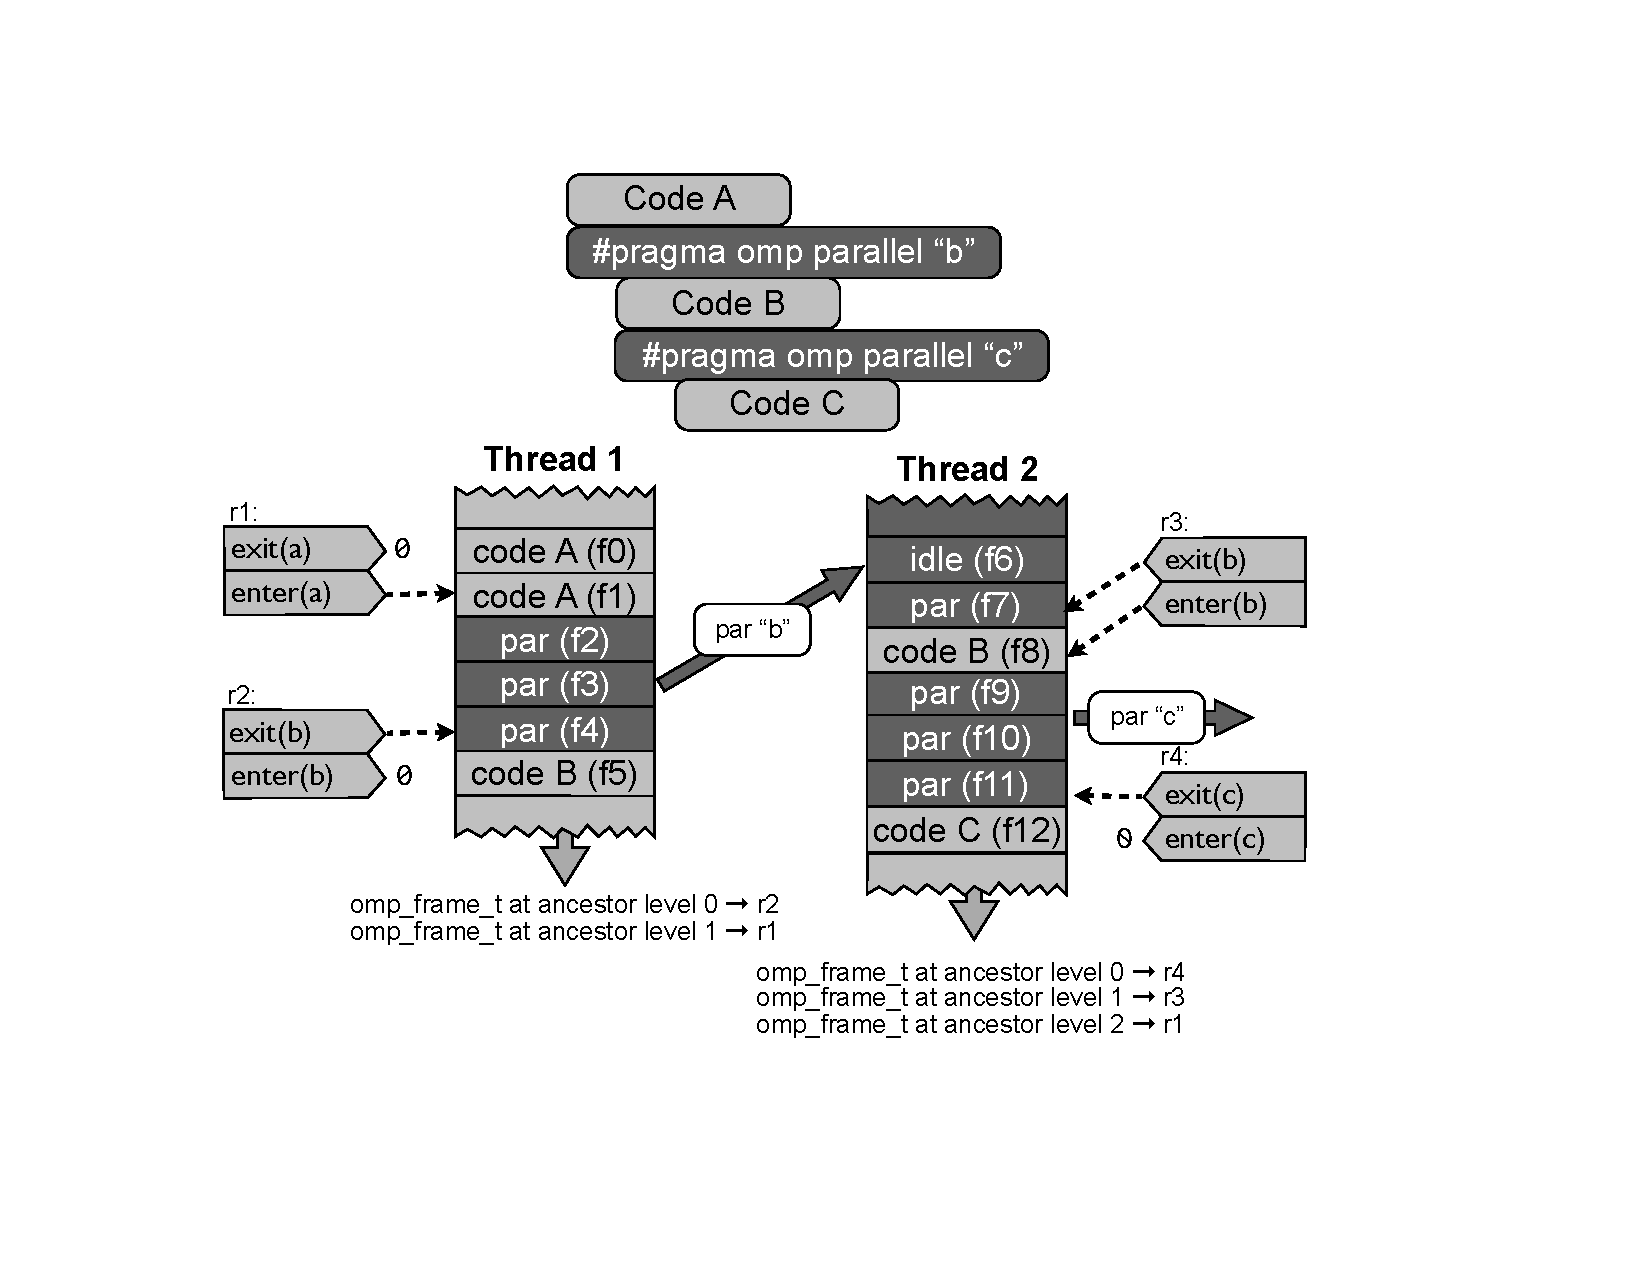
\includegraphics[width=4in]{appendices/callstack-cropped.pdf}
    \caption{Thread call stacks implementing nested parallelism
      annotated with frame information for the OMPT tool interface.}
    \label{fig:frame}
\end{figure}

The top half of Figure~\ref{fig:frame} illustrates a
conceptualization of a program executing a nested
parallel region, where code A, B, and C represent, respectively, one
or more procedure frames of code
associated with an initial task, an outer parallel region, and an inner parallel
region. The bottom half of Figure~\ref{fig:frame} illustrates the stacks of two
threads executing the nested parallel region.
In the illustration, stacks grow downward---a call to a function adds
a new frame to the stack below the frame of its caller.
When thread 1 encounters the outer-parallel
region ``b", it calls a routine in the OpenMP runtime to
create a new parallel region. The OpenMP runtime sets the
\plc{enter_frame} field in the \code{ompt_frame_t} for the initial
task executing code A to the canonical frame address of frame f1---the user frame in the initial task
that calls the runtime. The \code{ompt_frame_t} for the initial task
is labeled \plc{r1} in Figure~\ref{fig:frame}. In this figure, three
consecutive runtime system frames, labeled ``par'' with frame
identifiers f2--f4, are on the stack.  Before starting the implicit
task for parallel region ``b" in thread 1, the runtime sets the
\plc{exit_frame} in the implicit task's \code{ompt_frame_t} (labeled
\plc{r2}) to the canonical frame address of frame f4. Execution of application code for parallel region
``b'' begins on thread 1 when the runtime system invokes application
code B (frame f5) from frame f4.

Let us focus now on thread 2, an OpenMP thread. Figure~\ref{fig:frame}
shows this worker executing work for the outer-parallel region ``b."
On the OpenMP thread's stack is a runtime frame labeled ``idle,''
where the OpenMP thread waits for work.  When work becomes available,
the runtime system invokes a function to dispatch it. While
dispatching parallel work might involve a chain of several calls, here
we assume that the length of this chain is 1 (frame f7).  Before
thread 2 exits the runtime to execute an implicit task for parallel
region ``b,'' the runtime sets the \plc{exit_frame} field of the
implicit task's \code{ompt_frame_t} (labeled \plc{r3}) to the canonical frame address of frame f7.
When thread 2 later encounters the inner-parallel region ``c," as
execution returns to the runtime, the runtime fills in the
\plc{enter_frame} field of the current task's \code{ompt_frame_t}
(labeled \plc{r3}) to the canonical frame address of frame f8---the frame that invoked the
runtime. Before the task for parallel region ``c'' is invoked on
thread 2, the runtime system sets the \plc{exit_frame} field of the
\code{ompt_frame_t} (labeled \plc{r4}) for the implicit task for
``c'' to the canonical frame address of frame f11. Execution of application code for parallel region
``c'' begins on thread 2 when the runtime system invokes application
code C (frame f12) from frame f11.


Below the stack for each thread in Figure~\ref{fig:frame}, the figure
shows the \code{ompt_frame_t} information obtained by calls to
\code{ompt_get_task_info} made on each thread for the stack state
shown. We show the ID of the \code{ompt_frame_t} object returned at
each ancestor level. Note that thread 2 has task frame information for
three levels of tasks, whereas thread 1 has only two.

\crossreferences
\begin{itemize}
\item \code{ompt_frame_t}, see \specref{sec:ompt_frame_t}.
\item \code{ompt_get_task_info_t}, see \specref{sec:ompt_get_task_info_t}.
\end{itemize}


% This is the end of appendix-frames.tex


    % This is appendix-frames.tex of the OpenMP specification.
% This is an included file. See the master file for more information.
%
% When editing this file:
%
%    1. To change formatting, appearance, or style, please edit openmp.sty.
%
%    2. Custom commands and macros are defined in openmp.sty.
%
%    3. Be kind to other editors -- keep a consistent style by copying-and-pasting to
%       create new content.
%
%    4. We use semantic markup, e.g. (see openmp.sty for a full list):
%         \code{}     % for bold monospace keywords, code, operators, etc.
%         \plc{}      % for italic placeholder names, grammar, etc.
%
%    5. Other recommendations:
%         Use the convenience macros defined in openmp.sty for the minor headers
%         such as Comments, Syntax, etc.
%
%         To keep items together on the same page, prefer the use of 
%         \begin{samepage}.... Avoid \parbox for text blocks as it interrupts line numbering.
%         When possible, avoid \filbreak, \pagebreak, \newpage, \clearpage unless that's
%         what you mean. Use \needspace{} cautiously for troublesome paragraphs.
%
%         Avoid absolute lengths and measures in this file; use relative units when possible.
%         Vertical space can be relative to \baselineskip or ex units. Horizontal space
%         can be relative to \linewidth or em units.
%
%         Prefer \emph{} to italicize terminology, e.g.:
%             This is a \emph{definition}, not a placeholder.
%             This is a \plc{var-name}.
%


\chapter{Interaction Diagram of OMPD Components}
\index{ompd diagram}
\label{chap:ompd_diagram}


   \begin{figure}[h]
    \centering
        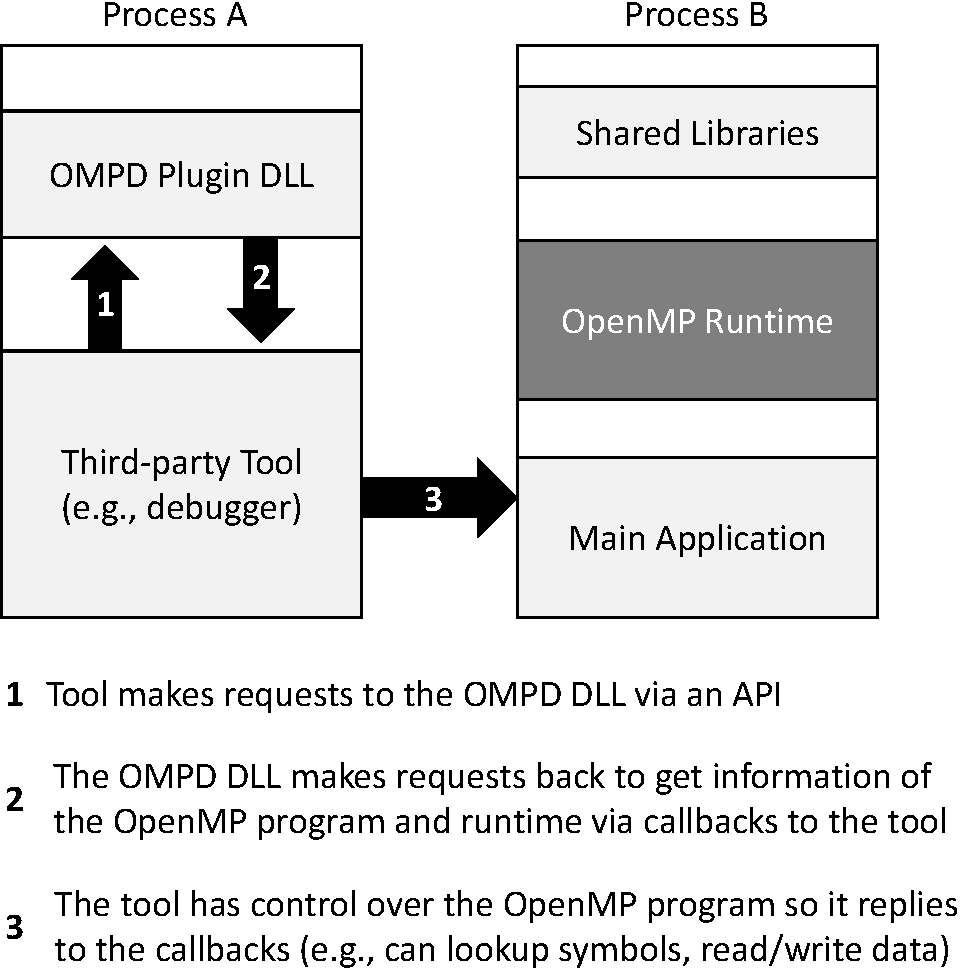
\includegraphics[width=3.5in]{appendices/ompd_diagram.pdf}
    \caption{Interaction Diagram of OMPD Components}
    \label{fig:ompd_diagram}
\end{figure}

The figure shows how the different components of OMPD fit together. The third-party tool loads 
the OMPD plugin
that matches the OpenMP runtime being used by the OpenMP program. The 
plugin exports the API defined in
\specref{sec:ompd:ompd-overview}, which the tool uses to get 
OpenMP information about the 
OpenMP program. The OMPD
plugin will need to look up the symbols, or read data out of the 
OpenMP program. It does not do this directly,
but instead asks the tool to perform these operations 
for it using a callback interface exported
by the tool.

This architectural layout insulates the tool from the details of the 
internal structure of the
OpenMP runtime. Similarly, the OMPD plugin does not need to be 
concerned about how to access
the OpenMP program. Decoupling the plugin and tool in this 
way allows for flexibility in how the OpenMP program and tool are deployed, so that, for example, 
there is no requirement that tool and OpenMP program
execute on the same machine.

\crossreferences
\begin{itemize}
\item See \specref{sec:ompd:ompd-overview}.
\end{itemize}


    % This is features_history.tex (Appendix E) of the OpenMP specification.
% This is an included file. See the master file for more information.
%
% When editing this file:
%
%    1. To change formatting, appearance, or style, please edit openmp.sty.
%
%    2. Custom commands and macros are defined in openmp.sty.
%
%    3. Be kind to other editors -- keep a consistent style by copying-and-pasting to
%       create new content.
%
%    4. We use semantic markup, e.g. (see openmp.sty for a full list):
%         \code{}     % for bold monospace keywords, code, operators, etc.
%         \plc{}      % for italic placeholder names, grammar, etc.
%
%    5. There are environments that provide special formatting, e.g. language bars.
%       Please use them whereever appropriate.  Examples are:
%
%         \begin{fortranspecific}
%         This is text that appears enclosed in blue language bars for Fortran.
%         \end{fortranspecific}
%
%         \begin{note}
%         This is a note.  The "Note -- " header appears automatically.
%         \end{note}
%
%    6. Other recommendations:
%         Use the convenience macros defined in openmp.sty for the minor headers
%         such as Comments, Syntax, etc.
%
%         To keep items together on the same page, prefer the use of
%         \begin{samepage}.... Avoid \parbox for text blocks as it interrupts line numbering.
%         When possible, avoid \filbreak, \pagebreak, \newpage, \clearpage unless that's
%         what you mean. Use \needspace{} cautiously for troublesome paragraphs.
%
%         Avoid absolute lengths and measures in this file; use relative units when possible.
%         Vertical space can be relative to \baselineskip or ex units. Horizontal space
%         can be relative to \linewidth or em units.
%
%         Prefer \emph{} to italicize terminology, e.g.:
%             This is a \emph{definition}, not a placeholder.
%             This is a \plc{var-name}.%


\chapter{Features History}
\index{features history}
\index{history of features}
\label{chap:Features History}
This appendix summarizes the major changes between recent versions of the OpenMP
API since version 2.5.

\section{Deprecated Features}
\index{deprecated features}
\label{chap:Deprecated Features}

The following features have been deprecated:

\begin{itemize}
\item the \plc{nest-var} ICV;
\item the \code{OMP_NESTED} environment variable;
\item the \code{omp_set_nested} and \code{omp_get_nested} routines;
\item the C/C++ type \code{omp_lock_hint_t} and the corresponding Fortran kind \code{omp_hint_hint_kind};
\item and the lock hint constants \code{omp_lock_hint_none}, \code{omp_lock_hint_uncontended}, \code{omp_lock_hint_contended}, \code{omp_lock_hint_nonspeculative}, and \code{omp_lock_hint_speculative}.
\end{itemize}



\section{Version 4.5 to 5.0 Differences}
\label{sec:Version 4.5 to 5.0 Differences}
\begin{itemize}
\item Stubs for Runtime Library Routines(previously Appendix A) were moved to a separate document.
\item Interface Declarations (previously Appendix B) were moved to a separate document.

\item The memory model was extended to distinguish different types of flush
      operations according to specified flush properties (see
      \specref{subsec:The Flush Operation}) and to define a happens
      before order based on synchronizing flush operations
      (see \specref{subsec:happens-before}).

\item Various changes throughout the specification were made to provide
      initial support of C11, C++11, C++14 and Fortran 2008 (see
      \specref{sec:normative references}).

\item Support for several features of Fortran 2003 was added (see
      \specref{sec:normative references} for features that are still
      not supported).

\item The list items allowable in a \code{depend} clause on a task generating
      construct was extended, including for C/C++ allowing any \plc{lvalue}
      expression (see \specref{sec:Directive Format} and
      \specref{subsec:depend Clause}).

\item The \code{requires} directive (see \specref{sec:requires Directive}) was
      added to support applications that require implementation-specific
      features generally and shared memory across devices specifically.

\item The \plc{target-offload-var} internal control variable (see
      \specref{sec:Internal Control Variables}) and the
      \code{OMP_TARGET_OFFLOAD} environment variable (see
      \specref{sec:OMP_TARGET_OFFLOAD}) were added to support runtime
      control of the execution of device constructs.

\item The default value of the \plc{nest-var} ICV was changed from \plc{false}
      to implementation defined (see \specref{subsec:ICV Initialization}).
      The \plc{nest-var} ICV (see \specref{subsec:ICV Descriptions}), the
      \code{OMP_NESTED} environment variable (see \specref{sec:OMP_NESTED}),
      and the \code{omp_set_nested} and \code{omp_get_nested} routines
      were deprecated (see \specref{subsec:omp_set_nested} and
      \specref{subsec:omp_get_nested}).

\item Iterators (see \specref{sec:iterators}) were added to express that an
      expression in a list may expand to multiple expressions.

\item The \code{teams} construct (see \specref{sec:teams Construct}) was was
      extended to also support host execution without surrounding \code{target}
      construct (see \specref{subsec:target Construct}).

\item The \plc{relational-op} in the canonical loop form for C/C++ was
      extended to include != (see \specref{sec:Canonical Loop Form}).

\item The collapse of associated loops that are imperfectly nested loops
      was defined for the loop (see \specref{subsec:Loop Construct}),
      \code{simd} (see \specref{subsec:simd Construct}), \code{taskloop}
      (see \specref{subsec:taskloop Construct}) and \code{distribute} (see
      \specref{subsec:distribute simd Construct}) constructs.

\item SIMD constructs (see \specref{sec:SIMD Constructs}) were extended
      to allow the use of \code{atomic} constructs within them.

\item The \code{if} and \code{nontemporal} clauses were added to the 
      \code{simd} construct (see \specref{subsec:simd Construct}).

\item The \code{concurrent} construct was added to support compiler
      optimization of loops for which iterations may run in any order
      concurrently (see \specref{sec:concurrent Construct}).

\item To support task reductions, the \code{task} (see
      \specref{subsec:task Construct}) and \code{target} (see
      \specref{subsec:target Construct}) constructs were extended to
      accept the the \code{in_reduction} clause (see
      \specref{subsubsec:in_reduction clause}) and the \code{taskgroup}
      construct (see \specref{subsec:taskgroup Construct}) was extended
      to accept the \code{task_reduction} clause
      \specref{subsubsec:task_reduction clause}).

\item The \code{affinity} clause was added to the \code{task} construct
      (see \specref{subsec:task Construct}) to support hints that indicate 
      data affinity of explicit tasks. 

\item To support taskloop reductions, the \code{taskloop} (see
      \specref{subsec:taskloop Construct}) and \code{taskloop simd} (see
      \specref{subsec:taskloop simd Construct}) constructs were extended
      to accept the \code{reduction} (see \specref{subsubsec:reduction clause})
      and \code{in_reduction} (see \specref{subsubsec:in_reduction clause})
      clauses.

\item To support mutually exclusive inout sets, a \code{mutexinoutset}
      \plc{dependence-type} was added to the \code{depend} clause (see
      \specref{subsec:Task Scheduling} and \specref{subsec:depend Clause}).

\item Predefined memory spaces (see \specref{subsec:Memory Spaces}), 
      predefined memory allocators and allocator traits (see 
      \specref{subsec:Memory Allocators}) and directives, clauses (see 
      \specref{sec:Memory Management Directives} and API routines (see 
      \specref{sec:Memory Management Routines}) to use them were added 
      to support different kinds of memories.

\item To reduce programmer effort implicit declare target directives for
      some functions (C, C++, Fortran) and subroutines (Fortran) were added
      (see \specref{subsec:target Construct} and
      \specref{subsec:declare target Directive}).

\item The \code{target update} (see \specref{subsec:target update
      Construct}) construct was modified to allow array sections that
      specify discontiguous storage.
      
\item Support for nested \code{declare}~\code{target} directives was added
      (see \specref{subsec:declare target Directive}).

\item The \code{implements} clause was added to the
      \code{declare}~\code{target} directive to support the use of
      device-specific function implementations (see
      \specref{subsec:declare target Directive}).

\item The \code{declare}~\code{mapper} directive was added to support
      mapping of complicated data types (see
      \specref{subsec:declare mapper Directive}).

\item The \code{depend} clause was added to the \code{taskwait} construct
      (see \specref{subsec:taskwait Construct}).

\item To support acquire and release semantics with weak memory ordering, the
      \code{acq_rel}, \code{acquire}, and \code{release} clauses were added to
      the \code{atomic} construct (see \specref{subsec:atomic Construct}) and
      \code{flush} construct (see \specref{subsec:flush Construct}).

\item The \code{atomic} construct was extended with the \code{hint} clause
      (see \specref{subsec:atomic Construct}).

\item The \code{depend} clause (see \specref{subsec:depend Clause}) was
      extended to support iterators.

\item Lock hints were renamed to synchronization hints, and the
      old names were deprecated (see \specref{subsec:Synchronization Hints}).

\item To support conditional assignment to lastprivate variables, the
      \code{conditional} modifier was added to the \code{lastprivate}
      clause (see \specref{subsubsec:lastprivate clause}).

\item The description of the \code{map} clause was modified to clarify how
      structure members are mapped. (see \specref{subsec:map Clause}).

\item The capability to map pointer variables (C/C++) and assign the
      address of device memory that is mapped by an array section to them
      was added (see \specref{subsec:map Clause}).

\item The \code{defaultmap} clause (see \specref{subsubsec:defaultmap clause})
      was extended to allow selecting the mapping or data sharing attributes for
      any of the scalar, aggregate, pointer or allocatable classes on a
      per-region basis. Additionally it accepts the \code{none} parameter to support the
      requirement that all variables all variables referenced in the
      construct must be explicitly mapped or privatized.

\item The \code{omp_get_device_num} runtime routine
      (see \specref{subsec:omp_get_device_num}) was added to support
      determination of the device on which a thread is executing.

\item Runtime routines (see \specref{subsec:omp_set_affinity_format},
      \specref{subsec:omp_get_affinity_format},
      \specref{subsec:omp_display_affinity}, and
      \specref{subsec:omp_capture_affinity}) and environment variables
      (see \specref{sec:OMP_DISPLAY_AFFINITY} and
      \specref{sec:OMP_AFFINITY_FORMAT}) were added to provide OpenMP
      thread affinity information.

\item The \code{omp_get_device_num} runtime routine
      (see \specref{subsec:omp_get_device_num}) was added to support
      determination of the device on which a thread is executing.

\item Support for a first-party tool interface (see
      \specref{sec:ompt-overview}) was added.

\item Support for a third-party tool interface (see
      \specref{sec:ompd-overview}) was added.

\item Support for controlling offloading behavior with the
      \code{OMP_TARGET_OFFLOAD} environment variable was added
      (see  \specref{sec:OMP_TARGET_OFFLOAD}).

\end{itemize}


\section{Version 4.0 to 4.5 Differences}
\label{sec:Version 4.0 to 4.5 Differences}
\begin{itemize}
\item Support for several features of Fortran 2003 was added (see
      \specref{sec:normative references} for features that are still
      not supported).

\item A parameter was added to the \code{ordered} clause of the loop construct
      (see \specref{subsec:Loop Construct}) and clauses were added to the
      \code{ordered} construct (see \specref{subsec:ordered Construct}) to
      support doacross loop nests and use of the \code{simd} construct on
      loops with loop-carried backward dependences.

\item The \code{linear} clause was added to the loop construct
      (see \specref{subsec:Loop Construct}).

\item The \code{simdlen} clause was added to the \code{simd} construct
      (see \specref{subsec:simd Construct}) to support specification of
      the exact number of iterations desired per SIMD chunk.

\item The \code{priority} clause was added to the \code{task} construct
      (see \specref{subsec:task Construct}) to support hints that specify
      the relative execution priority of explicit tasks. The
      \code{omp_get_max_task_priority} routine was added to return
      the maximum supported priority value (see
      \specref{subsec:omp_get_max_task_priority}) and the
      \code{OMP_MAX_TASK_PRIORITY} environment variable was added to
      control the maximum priority value allowed (see
      \specref{sec:OMP_MAX_TASK_PRIORITY}).

\item Taskloop constructs (see \specref{subsec:taskloop Construct} and
      \specref{subsec:taskloop simd Construct}) were added to support
      nestable parallel loops that create OpenMP tasks.

\item To support interaction with native device implementations, the
      \code{use_device_ptr} clause was added to the \code{target data}
      construct (see \specref{subsec:target data Construct}) and the
      \code{is_device_ptr} clause was added to the \code{target} construct
      (see \specref{subsec:target Construct}).

\item The \code{nowait} and \code{depend} clauses were added to the
      \code{target} construct (see \specref{subsec:target Construct})
      to improve support for asynchronous execution of \code{target} regions.

\item The \code{private}, \code{firstprivate} and \code{defaultmap} clauses
      were added to the \code{target} construct (see \specref{subsec:target
      Construct}).

\item The \code{declare}~\code{target} directive was extended to allow
      mapping of global variables to be deferred to specific device
      executions and to allow an \plc{extended-list}
      to be specified in C/C++ (see \specref{subsec:declare target Directive}).

\item To support unstructured data mapping for devices, the
      \code{target enter data} (see \specref{subsec:target enter data
      Construct}) and \code{target exit data} (see \specref{subsec:target
      exit data Construct}) constructs were added and the \code{map} clause
      (see \specref{subsec:map Clause}) was updated.

\item To support a more complete set of device construct shortcuts, the
      \code{target}~\code{parallel}
      (see \specref{subsec:target parallel Construct}),
      target parallel loop
      (see \specref{subsec:Target Parallel Loop Construct}),
      target parallel loop SIMD
      (see \specref{subsec:Target Parallel Loop SIMD Construct}),
      and \code{target}~\code{simd}
      (see \specref{subsec:target simd Construct}),
      combined constructs were added.

\item The \code{if} clause was extended to take a
      \plc{directive-name-modifier} that allows it to apply
      to combined constructs (see \specref{sec:if Clause}).

\item The \code{hint} clause was addded to the \code{critical} construct
      (see \specref{subsec:critical Construct}).

\item The \code{source} and \code{sink} dependence types were added to the
      \code{depend} clause (see \specref{subsec:depend Clause}) to support
      doacross loop nests.

\item The implicit data-sharing attribute for scalar variables in
      \code{target} regions was changed to \code{firstprivate} (see
      \specref{subsubsec:Data-sharing Attribute Rules for Variables
      Referenced in a Construct}).

\item Use of some C++ reference types was allowed in some data sharing
      attribute clauses (see \specref{subsec:Data-Sharing Attribute Clauses}).

\item Semantics for reductions on C/C++ array sections were added and
      restrictions on the use of arrays and pointers in reductions were
      removed (see \specref{subsubsec:reduction clause}).

\item The \code{ref}, \code{val}, and \code{uval} modifiers were added to the
      \code{linear} clause (see \specref{subsubsec:linear clause}).

\item Support was added to the map clauses to handle structure elements
	(see \specref{subsec:map Clause}).

\item Query functions for OpenMP thread affinity were added (see
      \specref{subsec:omp_get_num_places} to \specref{subsec:omp_get_partition_place_nums}).

\item The lock API was extended with lock routines that support storing a hint
      with a lock to select a desired lock implementation for a lock's
      intended usage by the application code (see
      \specref{subsec:omp_init_lock_with_hint and omp_init_nest_lock_with_hint}).

\item Device memory routines were added to allow explicit allocation,
      deallocation, memory transfers and memory associations (see
      \specref{sec:Device Memory Routines}).

\item C/C++ Grammar (previously Appendix B) was moved to a separate document.
\end{itemize}



\section{Version 3.1 to 4.0 Differences}
\label{sec:Version 3.1 to 4.0 Differences}
\begin{itemize}
\item Various changes throughout the specification were made to provide initial support of
Fortran 2003 (see
\specref{sec:normative references}).

\item C/C++ array syntax was extended to support array sections (see
\specref{sec:Array Sections}).

\item The \code{proc_bind} clause (see
\specref{subsec:Controlling OpenMP Thread Affinity}),
the \code{OMP_PLACES}
environment variable (see
\specref{sec:OMP_PLACES}), and the \code{omp_get_proc_bind}
runtime routine (see
\specref{subsec:omp_get_proc_bind})
were added to support thread
affinity policies.

\item SIMD constructs were added to support SIMD parallelism (see
\specref{sec:SIMD Constructs}).

\item Device constructs (see
\specref{sec:Device Constructs}),
the \code{OMP_DEFAULT_DEVICE}
environment variable (see
\specref{sec:OMP_DEFAULT_DEVICE}), the
\code{omp_set_default_device}, \code{omp_get_default_device},
\code{omp_get_num_devices}, \code{omp_get_num_teams}, \code{omp_get_team_num}, and
\code{omp_is_initial_device} routines were added to support execution on devices.

\item Implementation defined task scheduling points for untied tasks were removed (see
\specref{subsec:Task Scheduling}).

\item The \code{depend} clause (see
\specref{subsec:depend Clause})
was added to support task dependences.

\item The \code{taskgroup} construct (see
\specref{subsec:taskgroup Construct}) was added to support
more flexible deep task synchronization.

\item The \code{reduction} clause (see
\specref{subsubsec:reduction clause}) was extended and the
\code{declare}~\code{reduction} construct (see
\specref{sec:declare reduction Directive}) was added to
support user defined reductions.

\item The \code{atomic} construct (see
\specref{subsec:atomic Construct}) was extended to support
atomic swap with the \code{capture} clause, to allow new atomic update and capture
forms, and to support sequentially consistent atomic operations with a new \code{seq_cst}
clause.

\item The \code{cancel} construct (see
\specref{subsec:cancel Construct}), the \code{cancellation}~\code{point} construct (see
\specref{subsec:cancellation point Construct}),
the \code{omp_get_cancellation}
runtime routine (see
\specref{subsec:omp_get_cancellation})
and the \code{OMP_CANCELLATION}
environment variable (see
\specref{sec:OMP_CANCELLATION}) were added to support the
concept of cancellation.

\item The \code{OMP_DISPLAY_ENV} environment variable (see
\specref{sec:OMP_DISPLAY_ENV}) was
added to display the value of ICVs associated with the OpenMP environment
variables.

\item Examples (previously Appendix A) were moved to a separate document.
\end{itemize}






\section{Version 3.0 to 3.1 Differences}
\label{sec:Version 3.0 to 3.1 Differences}
\begin{itemize}
\item The \code{final} and \code{mergeable} clauses (see
\specref{subsec:task Construct}) were added to
the \code{task} construct to support optimization of task data environments.

\item The \code{taskyield} construct (see
\specref{subsec:taskyield Construct}) was added to allow
user-defined task scheduling points.

\item The \code{atomic} construct (see
\specref{subsec:atomic Construct}) was extended to include
\code{read}, \code{write}, and \code{capture} forms, and an \code{update} clause was added to apply
the already existing form of the \code{atomic} construct.

\item Data environment restrictions were changed to allow \code{intent(in)} and
\code{const}-qualified types for the \code{firstprivate} clause (see
\specref{subsubsec:firstprivate clause}).

\item Data environment restrictions were changed to allow Fortran pointers in
\code{firstprivate} (see
\specref{subsubsec:firstprivate clause})
and \code{lastprivate} (see
\specref{subsubsec:lastprivate clause}).

\item New reduction operators \code{min} and \code{max} were added for C and C++

\item The nesting restrictions in
\specref{sec:Nesting of Regions} were clarified to disallow
closely-nested OpenMP regions within an \code{atomic} region. This allows an \code{atomic}
region to be consistently defined with other OpenMP regions so that they include all
code in the atomic construct.

\item The \code{omp_in_final} runtime library routine (see
\specref{subsec:omp_in_final}) was
added to support specialization of final task regions.

\item The \plc{nthreads-var} ICV has been modified to be a list of the number of threads to use
at each nested parallel region level. The value of this ICV is still set with the
\code{OMP_NUM_THREADS} environment variable (see
\specref{sec:OMP_NUM_THREADS}), but the
algorithm for determining the number of threads used in a parallel region has been
modified to handle a list (see
\specref{subsec:Determining the Number of Threads for a parallel Region}).

\item The \plc{bind-var} ICV has been added, which controls whether or not threads are bound
to processors (see
\specref{subsec:ICV Descriptions}).
The value of this ICV can be set with
the \code{OMP_PROC_BIND} environment variable (see
\specref{sec:OMP_PROC_BIND}).

\item Descriptions of examples (previously Appendix A) were expanded and
clarified.

\item Replaced incorrect use of \code{omp_integer_kind} in Fortran interfaces with
\code{selected_int_kind(8)}.
\end{itemize}







\section{Version 2.5 to 3.0 Differences}
\label{sec:Version 2.5 to 3.0 Differences}
The concept of tasks has been added to the OpenMP execution model (see
\specref{subsec:Tasking Terminology} and
\specref{sec:Execution Model}).

\begin{itemize}
\item The \code{task} construct (see
\specref{sec:Tasking Constructs})
has been added, which provides
a mechanism for creating tasks explicitly.

\item The \code{taskwait} construct (see
\specref{subsec:taskwait Construct}) has been added, which
causes a task to wait for all its child tasks to complete.

\item The OpenMP memory model now covers atomicity of memory accesses (see
\specref{subsec:Structure of the OpenMP Memory Model}).
The description of the behavior of \code{volatile} in terms of
\code{flush} was removed.

\item In Version 2.5, there was a single copy of the \plc{nest-var}, \plc{dyn-var}, \plc{nthreads-var} and
\plc{run-sched-var} internal control variables (ICVs) for the whole program. In Version
3.0, there is one copy of these ICVs per task (see
\specref{sec:Internal Control Variables}). As a result,
the \code{omp_set_num_threads}, \code{omp_set_nested} and \code{omp_set_dynamic}
runtime library routines now have specified effects when called from inside a
\code{parallel} region (see
\specref{subsec:omp_set_num_threads},
\specref{subsec:omp_set_dynamic} and
\specref{subsec:omp_set_nested}).

\item The definition of active \code{parallel} region has been changed: in Version 3.0 a
\code{parallel} region is active if it is executed by a team consisting of more than one
thread (see
\specref{subsec:OpenMP Language Terminology}).

\item The rules for determining the number of threads used in a \code{parallel} region have
been modified (see
\specref{subsec:Determining the Number of Threads for a parallel Region}).

\item In Version 3.0, the assignment of iterations to threads in a loop construct with a
\code{static} schedule kind is deterministic (see
\specref{subsec:Loop Construct}).

\item In Version 3.0, a loop construct may be associated with more than one perfectly
nested loop. The number of associated loops may be controlled by the \code{collapse}
clause (see
\specref{subsec:Loop Construct}).

\item Random access iterators, and variables of unsigned integer type, may now be used as
loop iterators in loops associated with a loop construct (see
\specref{subsec:Loop Construct}).

\item The schedule kind \code{auto} has been added, which gives the implementation the
freedom to choose any possible mapping of iterations in a loop construct to threads in
the team (see \specref{subsec:Loop Construct}).

\item Fortran assumed-size arrays now have predetermined data-sharing attributes (see
\specref{subsubsec:Data-sharing Attribute Rules for Variables Referenced in a Construct}).

\item In Fortran, \code{firstprivate} is now permitted as an argument to the \code{default}
clause (see
\specref{subsubsec:default clause}).

\item For list items in the \code{private} clause, implementations are no longer permitted to use
the storage of the original list item to hold the new list item on the master thread. If
no attempt is made to reference the original list item inside the \code{parallel} region, its
value is well defined on exit from the \code{parallel} region (see
\specref{subsubsec:private clause}).

\item In Version 3.0, Fortran allocatable arrays may appear in \code{private},
\code{firstprivate}, \code{lastprivate}, \code{reduction}, \code{copyin} and \code{copyprivate}
clauses. (see
\specref{subsec:threadprivate Directive},
\specref{subsubsec:private clause},
\specref{subsubsec:firstprivate clause},
\specref{subsubsec:lastprivate clause},
\specref{subsubsec:reduction clause},
\specref{subsubsec:copyin clause} and
\specref{subsubsec:copyprivate clause}).

\item In Version 3.0, static class members variables may appear in a \code{threadprivate}
directive (see
\specref{subsec:threadprivate Directive}).

\item Version 3.0 makes clear where, and with which arguments, constructors and
destructors of private and threadprivate class type variables are called (see
\specref{subsec:threadprivate Directive},
\specref{subsubsec:private clause},
\specref{subsubsec:firstprivate clause},
\specref{subsubsec:copyin clause} and
\specref{subsubsec:copyprivate clause}).

\item The runtime library routines \code{omp_set_schedule} and \code{omp_get_schedule}
have been added; these routines respectively set and retrieve the value of the
\plc{run-sched-var} ICV (see\\
\specref{subsec:omp_set_schedule} and
\specref{subsec:omp_get_schedule}).

\item The \plc{thread-limit-var} ICV has been added, which controls the maximum number of
threads participating in the OpenMP program. The value of this ICV can be set with
the \code{OMP_THREAD_LIMIT} environment variable and retrieved with the
\code{omp_get_thread_limit} runtime library routine (see
\specref{subsec:ICV Descriptions},
\specref{subsec:omp_get_thread_limit} and
\specref{sec:OMP_THREAD_LIMIT}).

\item The \plc{max-active-levels-var} ICV has been added, which controls the number of nested
active \code{parallel} regions. The value of this ICV can be set with the
\code{OMP_MAX_ACTIVE_LEVELS} environment variable and the
\code{omp_set_max_active_levels} runtime library routine, and it can be retrieved
with the \code{omp_get_max_active_levels} runtime library routine (see
\specref{subsec:ICV Descriptions},
\specref{subsec:omp_set_max_active_levels},
\specref{subsec:omp_get_max_active_levels} and
\specref{sec:OMP_MAX_ACTIVE_LEVELS}).

\item The \plc{stacksize-var} ICV has been added, which controls the stack size for threads that
the OpenMP implementation creates. The value of this ICV can be set with the
\code{OMP_STACKSIZE} environment variable (see
\specref{subsec:ICV Descriptions} and
\specref{sec:OMP_STACKSIZE}).

\item The \plc{wait-policy-var} ICV has been added, which controls the desired behavior of
waiting threads. The value of this ICV can be set with the \code{OMP_WAIT_POLICY}
environment variable (see
\specref{subsec:ICV Descriptions} and
\specref{sec:OMP_WAIT_POLICY}).

\item The \code{omp_get_level} runtime library routine has been added, which returns the
number of nested \code{parallel} regions enclosing the task that contains the call (see
\specref{subsec:omp_get_level}).

\item The \code{omp_get_ancestor_thread_num} runtime library routine has been added,
which returns, for a given nested level of the current thread, the thread number of the
ancestor (see
\specref{subsec:omp_get_ancestor_thread_num}).

\item The \code{omp_get_team_size} runtime library routine has been added, which returns,
for a given nested level of the current thread, the size of the thread team to which the
ancestor belongs (see
\specref{subsec:omp_get_team_size}).

\item The \code{omp_get_active_level} runtime library routine has been added, which
returns the number of nested, active \code{parallel} regions enclosing the task that
contains the call (see\linebreak \specref{subsec:omp_get_active_level}).

\item In Version 3.0, locks are owned by tasks, not by threads (see
\specref{sec:Lock Routines}).
\end{itemize}


% This is the end of appendix-E-FeaturesHistory.tex



    \nolinenumbers
    \cleardoublepage
    \phantomsection
    \addcontentsline{toc}{chapter}{Index}
    \printindex
\end{document}

